%%%%%%%%%%%%%%%%%%%%%%%%%%%%%%%%%%%%%%%%%%%%%%%%%%%%%%%%%%%%%%%
%% OXFORD THESIS TEMPLATE

% Use this template to produce a standard thesis that meets the Oxford University requirements for DPhil submission
%
% Originally by Keith A. Gillow (gillow@maths.ox.ac.uk), 1997
% Modified by Sam Evans (sam@samuelevansresearch.org), 2007
% Modified by John McManigle (john@oxfordechoes.com), 2015
% Modified by Ulrik Lyngs (ulrik.lyngs@cs.ox.ac.uk), 2018-, for use with R Markdown
%
% Ulrik Lyngs, 25 Nov 2018: Following John McManigle, broad permissions are granted to use, modify, and distribute this software
% as specified in the MIT License included in this distribution's LICENSE file.
%
% John commented this file extensively, so read through to see how to use the various options.  Remember that in LaTeX,
% any line starting with a % is NOT executed.  Several places below, you have a choice of which line to use
% out of multiple options (eg draft vs final, for PDF vs for binding, etc.)  When you pick one, add a % to the beginning of
% the lines you don't want.


%%%%% PAGE LAYOUT
% The most common choices should be below.  You can also do other things, like replacing "a4paper" with "letterpaper", etc.

% This one formats for two-sided binding (ie left and right pages have mirror margins; blank pages inserted where needed):
%\documentclass[a4paper,twoside]{templates/ociamthesis}
% This one formats for one-sided binding (ie left margin > right margin; no extra blank pages):
%\documentclass[a4paper]{ociamthesis}
% This one formats for PDF output (ie equal margins, no extra blank pages):
%\documentclass[a4paper,nobind]{templates/ociamthesis}

% As you can see from the uncommented line below, oxforddown template uses the a4paper size, 
% and passes in the binding option from the YAML header in index.Rmd:
\documentclass[a4paper, nobind]{templates/ociamthesis}


%%%%% ADDING LATEX PACKAGES
% add hyperref package with options from YAML %
\usepackage[pdfpagelabels]{hyperref}
% change the default coloring of links to something sensible
\usepackage{xcolor}

\definecolor{mylinkcolor}{RGB}{0,0,139}
\definecolor{myurlcolor}{RGB}{0,0,139}
\definecolor{mycitecolor}{RGB}{0,33,71}

\hypersetup{
  hidelinks,
  colorlinks,
  linktocpage=true,
  linkcolor=mylinkcolor,
  urlcolor=myurlcolor,
  citecolor=mycitecolor
}



% add float package to allow manual control of figure positioning %
\usepackage{float}

% enable strikethrough
\usepackage[normalem]{ulem}

% use soul package for correction highlighting
\usepackage{color, soul}
\definecolor{correctioncolor}{HTML}{CCCCFF}
\sethlcolor{correctioncolor}
\newcommand{\ctext}[3][RGB]{%
  \begingroup
  \definecolor{hlcolor}{#1}{#2}\sethlcolor{hlcolor}%
  \hl{#3}%
  \endgroup
}
\soulregister\ref7
\soulregister\cite7
\soulregister\autocite7
\soulregister\textcite7
\soulregister\pageref7

%%%%% FIXING / ADDING THINGS THAT'S SPECIAL TO R MARKDOWN'S USE OF LATEX TEMPLATES
% pandoc puts lists in 'tightlist' command when no space between bullet points in Rmd file,
% so we add this command to the template
\providecommand{\tightlist}{%
  \setlength{\itemsep}{0pt}\setlength{\parskip}{0pt}}
 
% UL 1 Dec 2018, fix to include code in shaded environments

% User-included things with header_includes or in_header will appear here
% kableExtra packages will appear here if you use library(kableExtra)
\usepackage{booktabs}
\usepackage{longtable}
\usepackage{array}
\usepackage{multirow}
\usepackage{wrapfig}
\usepackage{float}
\usepackage{colortbl}
\usepackage{pdflscape}
\usepackage{tabu}
\usepackage{threeparttable}
\usepackage{threeparttablex}
\usepackage[normalem]{ulem}
\usepackage{makecell}
\usepackage{xcolor}


%UL set section header spacing
\usepackage{titlesec}
% 
\titlespacing\subsubsection{0pt}{24pt plus 4pt minus 2pt}{0pt plus 2pt minus 2pt}


%UL set whitespace around verbatim environments
\usepackage{etoolbox}
\makeatletter
\preto{\@verbatim}{\topsep=0pt \partopsep=0pt }
\makeatother


%%%%%%% PAGE HEADERS AND FOOTERS %%%%%%%%%
\usepackage{fancyhdr}
\setlength{\headheight}{15pt}
\fancyhf{} % clear the header and footers
\pagestyle{fancy}
\renewcommand{\chaptermark}[1]{\markboth{\thechapter. #1}{\thechapter. #1}}
\renewcommand{\sectionmark}[1]{\markright{\thesection. #1}} 
\renewcommand{\headrulewidth}{0pt}

\fancyhead[LO]{\emph{\leftmark}} 
\fancyhead[RE]{\emph{\rightmark}} 

% UL page number position 
\fancyfoot[C]{\emph{\thepage}} %regular pages
\fancypagestyle{plain}{\fancyhf{}\fancyfoot[C]{\emph{\thepage}}} %chapter pages

% JEM fix header on cleared pages for openright
\def\cleardoublepage{\clearpage\if@twoside \ifodd\c@page\else
   \hbox{}
   \fancyfoot[C]{}
   \newpage
   \if@twocolumn\hbox{}\newpage
   \fi
   \fancyhead[LO]{\emph{\leftmark}} 
   \fancyhead[RE]{\emph{\rightmark}} 
   \fi\fi}


%%%%% SELECT YOUR DRAFT OPTIONS
% This adds a "DRAFT" footer to every normal page.  (The first page of each chapter is not a "normal" page.)

% IP feb 2021: option to include line numbers in PDF

% for line wrapping in code blocks
\usepackage{fvextra}
\DefineVerbatimEnvironment{Highlighting}{Verbatim}{breaklines,commandchars=\\\{\}}

% This highlights (in blue) corrections marked with (for words) \mccorrect{blah} or (for whole
% paragraphs) \begin{mccorrection} . . . \end{mccorrection}.  This can be useful for sending a PDF of
% your corrected thesis to your examiners for review.  Turn it off, and the blue disappears.
\correctionstrue


%%%%% BIBLIOGRAPHY SETUP
% Note that your bibliography will require some tweaking depending on your department, preferred format, etc.
% If you've not used LaTeX before, I recommend reading a little about biblatex/biber and getting started with it.
% If you're already a LaTeX pro and are used to natbib or something, modify as necessary.
% Either way, you'll have to choose and configure an appropriate bibliography format...


\usepackage[style=authoryear, sorting=nyt, backend=biber, maxcitenames=1, maxbibnames=20, uniquelist=false, firstinits=true, date=year, useprefix, doi=true, isbn=false, url=false, uniquename=false]{biblatex}
\newcommand*{\bibtitle}{Works Cited}

\addbibresource{bibliography/references.bib}
\addbibresource{bibliography/additional-references.bib}
\addbibresource{bibliography/bibtex.bib}


%CSL

% This makes the bibliography left-aligned (not 'justified') and slightly smaller font.
\renewcommand*{\bibfont}{\raggedright\small}


% Uncomment this if you want equation numbers per section (2.3.12), instead of per chapter (2.18):
%\numberwithin{equation}{subsection}


%%%%% THESIS / TITLE PAGE INFORMATION
% Everybody needs to complete the following:
\title{Ecology of Ticks and Microbes in\\
Australia Wildlife}
\author{Siobhon Lee Egan}
\qual{Bachelor of Science (Honours)}

% Master's candidates who require the alternate title page (with candidate number and word count)
% must also un-comment and complete the following three lines:

% Uncomment the following line if your degree also includes exams (eg most masters):
%\renewcommand{\submittedtext}{Submitted in partial completion of the}
% Your full degree name.  (But remember that DPhils aren't "in" anything.  They're just DPhils.)
\degree{Doctor of Philosophy}
% Term and year of submission, or date if your board requires (eg most masters)
\degreedate{2022}


%%%%% YOUR OWN PERSONAL MACROS
% This is a good place to dump your own LaTeX macros as they come up.

% To make text superscripts shortcuts
	\renewcommand{\th}{\textsuperscript{th}} % ex: I won 4\th place
	\newcommand{\nd}{\textsuperscript{nd}}
	\renewcommand{\st}{\textsuperscript{st}}
	\newcommand{\rd}{\textsuperscript{rd}}

%%%%% THE ACTUAL DOCUMENT STARTS HERE
\begin{document}

%%%%% CHOOSE YOUR LINE SPACING HERE
% This is the official option.  Use it for your submission copy and library copy:
\setlength{\textbaselineskip}{22pt plus2pt}
% This is closer spacing (about 1.5-spaced) that you might prefer for your personal copies:
%\setlength{\textbaselineskip}{18pt plus2pt minus1pt}

% You can set the spacing here for the roman-numbered pages (acknowledgements, table of contents, etc.)
\setlength{\frontmatterbaselineskip}{17pt plus1pt minus1pt}

% UL: You can set the line and paragraph spacing here for the separate abstract page to be handed in to Examination schools
\setlength{\abstractseparatelineskip}{13pt plus1pt minus1pt}
\setlength{\abstractseparateparskip}{0pt plus 1pt}

% UL: You can set the general paragraph spacing here - I've set it to 2pt (was 0) so
% it's less claustrophobic
\setlength{\parskip}{2pt plus 1pt}

%
% Customise title page
%
\def\crest{{
\includegraphics[width=5cm]{templates/mulogo.png}}}
\renewcommand{\university}{Murdoch University}
\renewcommand{\submittedtext}{This thesis is presented for the degree of}
\renewcommand{\thesistitlesize}{\fontsize{22pt}{28pt}\selectfont}
\renewcommand{\gapbeforecrest}{25mm}
\renewcommand{\gapaftercrest}{25mm}

%\def\unifoot{{\includegraphics[width=]{}}}

% Leave this line alone; it gets things started for the real document.
\setlength{\baselineskip}{\textbaselineskip}


%%%%% CHOOSE YOUR SECTION NUMBERING DEPTH HERE
% You have two choices.  First, how far down are sections numbered?  (Below that, they're named but
% don't get numbers.)  Second, what level of section appears in the table of contents?  These don't have
% to match: you can have numbered sections that don't show up in the ToC, or unnumbered sections that
% do.  Throughout, 0 = chapter; 1 = section; 2 = subsection; 3 = subsubsection, 4 = paragraph...

% The level that gets a number:
\setcounter{secnumdepth}{2}
% The level that shows up in the ToC:
\setcounter{tocdepth}{1}


%%%%% ABSTRACT SEPARATE
% This is used to create the separate, one-page abstract that you are required to hand into the Exam
% Schools.  You can comment it out to generate a PDF for printing or whatnot.

% JEM: Pages are roman numbered from here, though page numbers are invisible until ToC.  This is in
% keeping with most typesetting conventions.
\begin{romanpages}

% Title page is created here
\maketitle

%%%%% DEDICATION
\begin{dedication}
  For Rhys William John Egan
\end{dedication}

%%%%% ABSTRACT


\renewcommand{\abstracttitle}{Abstract}
\begin{abstract}
	Ticks (Ixodida) represent one of the most important vector groups affecting human and animal health, and in recent years there have been increasing concerns regarding the cause of tick-borne disease affecting Australians. Worldwide, wildlife health surveillance is recognised as a key tool for investigating tick-borne infections and a One Health approach is essential to understand the epidemiology of tick-associated microbes. Therefore, this research aimed to; i) identify ticks from Australian wildlife; ii) investigate bacteria and haemoprotozoa present in wildlife and ticks; and iii) characterise microbes and understand the interplay between host-microbe-tick. Molecular tools were used to assist in the identification of Australian ticks. Museum specimens of the human biting tick \emph{Amblyomma triguttatum} were used to investigate the molecular systematics of this species complex. A set of molecular barcodes was developed for Australian ticks, which was important for the accurate identification of immature life stages and cryptic species. Additionally, a novel 12S rDNA metabarcoding assay was developed for high throughput identification of ticks. Free-ranging animals and their ticks were sampled from urban and peri-urban areas. The bacterial and haemoprotozoan diversity was characterised using a combination of amplicon \hl{high-throughput sequencing}, targeted Sanger sequencing, and microscopy. Bacterial profiling generated over 100 million sequences. Statistical analysis using constrained ordination methods revealed blood, tick and tissues had distinct community signatures. A diverse range of tick associated microbes was identified, such as \emph{Anaplasmataceae}, \emph{Bartonellaceae}, \emph{Borreliaceae}, \emph{Coxiellaceae}, \emph{Midichloriaceae.} Overall, these microbes were rare in wildlife hosts and generally confined to specific sample types. In addition, eight species of haemoprotozoa were identified, including species within the genera \emph{Babesia}, \emph{Hepatozoon}, \emph{Theileria} and \emph{Trypanosoma.} Lastly, this study further confirmed the absence of northern hemisphere tick-borne pathogens and provided further evidence of the unique microbes present in Australian wildlife and ticks.
\end{abstract}




%%%%% ACKNOWLEDGEMENTS


\begin{acknowledgements}
 	Firstly I would like to thank my Principal Supervisor Dr.~Charlotte Oskam.
  I will forever be grateful for your fierce support and mentorship over these last few years.
  From the first email I sent all those years ago now, you have always been so generous with your time.
  I thank you dearly for your advice, kindness and guidance throughout this journey.

  To Prof.~Peter Irwin, thank you for welcoming me in and providing me the platform to explore the wonderful world of wildlife and parasites.
  It has been an honour to share in this project and I will forever be grateful at the unique chance to learn from you and share some great memories in the field.

  To Prof.~Una Ryan, your kindness and generosity truly is one-of-kind.
  Thank you for the support, opportunities and advice you have provided throughout this time.
  It has been a delight to learn from you and share in the delicious supply of baked good!

  A project like this is not possible without a small army of help. Completing a PhD project in wildlife zoonoses has been an honour.
  It has led me on a fantastic journey and granted me the pleasure of experiencing some wonderful place.

  A huge thank you to my Co-Supervisor Prof.~Peter Banks and to Casey Taylor at the University of Sydney. This project would not able been possible without you both.
  Thank you for being generous hosts and fantastic collaborators.
  An extended thank you to the Banks lab for support and assistance with field work.

  To Dr.~Jill Austen, a massive thank you for your loyal support and friendship.
  Thank you for generously welcoming me into the Austen family and making me feel so comfortable. You very quickly become fundamental to this project and I will be forever grateful for all you did to help achieve this.

  I owe a huge debt to Dr.~Amy Northover. It never crossed my mind to pursue research until our paths met, thank you for your mentorship and continued support. Thank you also to Sarah Keatley, many moons ago you so very patiently introduced me to the lab world and I have never look backed. Thank you both also for extended loaning of equipment during fieldwork times.

  Thank you to the Department of Biodiversity, Conservation and Attraction team at the Perth Hills and surrounds for allowing me to tag along during field sessions. In particular, to Rebecca Kay, Douglas Giles and Hannah Kilian. Thank you to Jade Kelly, Dr.~Amanda Barbosa and volunteers for assistance in fieldwork and sample collection.

  A special mention to Dr.~Joe Fontaine - early on in my PhD journey you provided some much valued direction, mentorship and extended connections. I thank you and the team for always obliging to collect ticks!

  To Dr.~Bruce Halliday, thank you for your warm hospitality at the Australian National Insect Collection in Canberra and always assisting in queries and requests for more ticks! I also thank Prof.~Ian Beveridge (Melbourne University), Dr.~Mark Harvey (Western Autsralian Museum), Dr.~Owen Seeman (Queensland Museum) for providing advice on and access to tick collections.

  Access to specimens and controls was vital for validation assays. I thank Dr.~Jill Austen, Dr.~Amanda Barbosa, Dr.~Andrea Paparini, A/Prof.~Chris Peacock and The Australian Rickettsial Reference Laboratory.

  A huge thank you to Dr.~Shane Tobe, not only for providing some valued lab equipment, but also for the extended opportunities and guidance. A big thank you to Frances Brigg and Dr.~David Berryman (Western Australian State Agricultural Biotechnology Centre) for access to equipment and sequencing. Thank you also to Dr.~David Chandler, Dr.~Christopher Noune and Dr.~Matthew Stevens (Australian Genomics Research Facility) for assistance with assays and sequencing. To the Pawsey Supercomputing Research Centre, especially the help desk team - thank you for the always speedy responses and assistance setting up computational workflows.

  An extended thank you to the Cryptick Lab group, members past and present. Thank you for the good cheer, coffee runs and friendship over the years.

  Finally to my family, who laid the foundation for me to make all this possible.
  To mum (Denice), Allan, Katie, Rhys and Luke I wouldn't be who I am today without you all. Your love and support makes up the heart and soul of this work.
  To my partner Ray, thank for you for being my biggest support and making it possible to reach the end of this journey.
  I know it has has not always been easy but thank you for pushing me forward and never letting me give in.
\end{acknowledgements}


%%%%% DECLARATION


\begin{declaration}
 	I \emph{Siobhon Lee Egan} verify that in submitting this thesis;

  \begin{itemize}
  \tightlist
  \item
    the thesis is my own account of the research conducted by me, except where other sources are fully acknowledged in the appropriate format,
  \item
    the extent to which the work of others has been used is documented by a percent allocation of work and signed by myself and my Principal Supervisor,
  \item
    the thesis contains as its main content work which has not been previously submitted for a degree at any university,
  \item
    the University supplied plagiarism software has been used to ensure the work is of the appropriate standard to send for examination,
  \item
    any editing and proof-reading by professional editors comply with the standards set out on the Graduate Research School website, and
  \item
    that all necessary ethics and safety approvals were obtained, including their relevant approval or permit numbers, as appropriate.
  \end{itemize}

  \vspace{3mm}

  \raggedright

  \begin{center}\rule{0.5\linewidth}{0.5pt}\end{center}

  Siobhon Lee Egan

  \emph{14th March 2022}
\end{declaration}


%%%%% MINI TABLES
% This lays the groundwork for per-chapter, mini tables of contents.  Comment the following line
% (and remove \minitoc from the chapter files) if you don't want this.  Un-comment either of the
% next two lines if you want a per-chapter list of figures or tables.
  \dominitoc % include a mini table of contents

% This aligns the bottom of the text of each page.  It generally makes things look better.
\flushbottom

% This is where the whole-document ToC appears:
\tableofcontents

\listoffigures
	\mtcaddchapter
  	% \mtcaddchapter is needed when adding a non-chapter (but chapter-like) entity to avoid confusing minitoc

% Uncomment to generate a list of tables:
\listoftables
  \mtcaddchapter
%%%%% LIST OF ABBREVIATIONS
% This example includes a list of abbreviations.  Look at text/abbreviations.tex to see how that file is
% formatted.  The template can handle any kind of list though, so this might be a good place for a
% glossary, etc.
% First parameter can be changed eg to "Glossary" or something.
% Second parameter is the max length of bold terms.
\begin{mclistof}{List of Abbreviations}{3.2cm}

\item[16S]

16S ribosomal RNA

\item[18S]

18S ribosomal RNA

\item[ANIC]

Australian National Insect Collection

\item[ASV]

Amplicon sequence variant

\item[bp]

Base pair

\item[BIC]

Bayesian Information Criterion

\item[BLAST]

Basic Local Alignment Search Tool

\item[COX1]

Cytochrome c oxidase subunit I

\item[DNA]

Deoxyribonucleic acid

\item[dNTP]

Deoxynucloside triphosphate

\item[EXB]

Extraction blank

\item[FISF]

Flinders Island/Australian spotted fever

\item[gDNA]

Genomic DNA

\item[gGAPDH]

Glycosomal glyceraldehyde phosphate dehydrogenase gene

\item[GTR]

General time reversible

\item[HTS]

High-throughput sequencing

\item[Hz]

Hertz

\item[ITS2]

Internal transcribed spacer 2 region

\item[LB]

Lyme Borreliosis

\item[MCMC]

Markov chain Monte Carlo

\item[MDS]

Multidimensional scaling plot

\item[MgCl2]

Magnesium chloride

\item[min(s)]

Minute(s)

\item[mL]

Millilitre

\item[ML]

Maximum likelihood

\item[MLST]

Multi-locu sequence typing

\item[mM]

Millimolar

\item[mt]

Mitochondrial gene

\item[n]

Samlpe number

\item[NCBI]

National Centre for Biotechnology Information

\item[NJ]

Neighbour joining

\item[NSW]

New South Wales

\item[NT]

Northern Territory

\item[NTC]

No-template control

\item[Nu]

Nuclear gene

\item[OTU]

Operational Taxonomic Unit

\item[PCR]

Polymerase chain reaction

\item[QIIME2]

Quantitative Insights Into Microbial Ecology

\item[QLD]

Queensland

\item[QTT]

Queensland tick typhus

\item[OTU]

Operational Taxonomic Units

\item[rDNA]

Ribosomal deoxyribonucleic acid

\item[rRNA]

Ribosomal ribonucleic acid

\item[SA]

South Australia

\item[sec(s)]

Second(s)

\item[SFG]

Spotted fever group

\item[SNP]

Single nucleotide polymorphism

\item[sp.]

Species singular

\item[spp.]

Species multiple

\item[ssp.]

Subspecies

\item[TAS]

Tasmania

\item[Taq]

Thermus aquaticus deoxyribonucleic acid polymerase

\item[TBD]

Tick-borne disease

\item[TBP]

Tick-borne pathogen

\item[U]

Unit

\item[USA]

United States of America

\item[UV]

Ultraviolet

\item[VIC]

Victoria

\item[WA]

Western Australia

\item[WGS]

Whole genome sequencing

\item[ZOTU]

Zero-radius Operational Taxonomic Units

\end{mclistof} 


% The Roman pages, like the Roman Empire, must come to its inevitable close.
\end{romanpages}

%%%%% CHAPTERS
% Add or remove any chapters you'd like here, by file name (excluding '.tex'):
\flushbottom

% all your chapters and appendices will appear here
\hypertarget{preface-material}{%
\chapter*{Preface material}\label{preface-material}}
\addcontentsline{toc}{chapter}{Preface material}

\adjustmtc 
\chaptermark{Preface}

\hypertarget{thesis-format}{%
\section*{Thesis format}\label{thesis-format}}
\addcontentsline{toc}{section}{Thesis format}

This thesis has been written to present data collected during the degree of Doctor of Philosophy as a coherent piece of work incorporating a series of stand-alone manuscripts.
Each manuscript is written according to the authorship guidelines of the journal that the manuscript is accepted for publication, submitted for review, or will be submitted to in the future.
A statement of author attribution precedes each manuscript.
All chapters are presented in a similar format with continuous referencing and table and figure numbering to maintain the continuity of the document.

This thesis is comprised of 7 chapters.
Chapter \ref{litrev} comprises a literature review with an overview of ticks, tick-borne diseases and microorganisms.
In particular the review focuses on an Australian context and discusses the role of wildlife in the sylvatic cycle of microbes.
Towards the end of chapter one the thesis aims are detailed \ref{thesis-aims}.\\
The research chapters (2--6) are presented as individual scientific manuscripts and each contain their own abstract, introduction, materials and methods, results, and discussion.
It is noted that as each research chapter is stand alone there are some repetitive aspects to this thesis.
Modifications have been made to ensure consistency throughout this thesis and as such work presented here may differ slightly from any associated published work.
The general discussion, chapter \ref{gendiscussion} ties together major themes and findings presented in this thesis and provides a critical review on limitations and future directions.
To reduce redundancy some topics are not discussed in detail within the literature review and instead are included within the chapters.

All relevant data is made publicly available within this thesis.
Data has been deposited to relevant repositories.
Nucleotide sequence data has been deposited to GenBank, raw Illumina MiSeq sequence data has been deposited to the NCBI sequence read archive (SRA).
A data availability statement is provided at the start of each chapter.
Additional tables, figures and information are available in the Supplementary Material \ref{supplementary-material}.

\textbf{Scientific nomenclature}

Scientific names of ticks have been abbreviated as per \textcite{dantas-torresStandardizationAbbreviationsGenus2008} (typically utilising the first two letters of the genus, e.g.~\emph{Ixodes holocyclus} - \emph{Ix. holocyclus}).
In order to avoid confusion between two protozoal species of the genera \emph{Trypanosoma} and \emph{Theileria} the abbreviated notation of \emph{Tr.} and \emph{Th.} respectively has been used.
For consistency these abbreviations have been used throughout the thesis and as a result may differ from published versions.

Mammal common and scientific names follow \textcite{jacksonTaxonomyAustralianMammals2015}, except where there have since been changes published in the scientific literature.
Where relevant previous mammal names (common or scientific) are included (denoted by \emph{syn.}); these have been included in cases where the publication cited used different taxa name to those currently accepted, or as deemed relevant.

\hypertarget{funding-support}{%
\section*{Funding \& Support}\label{funding-support}}
\addcontentsline{toc}{section}{Funding \& Support}

This study was support by the Australian Research Council (LP160100200), Bayer HealthCare (Germany) and Bayer Australia.
Funding was also obtained by The Holsworth Wildlife Research Endowment administered by The Ecological Society of Australia.
This work was supported by resources provided by the Pawsey Supercomputing Centre with funding from the Australian Government and the Government of Western Australia.
This research was supported by an Australian Government Research Training Program (RTP) Scholarship.

As this thesis includes a number of collaborative projects any additional project funding or support is outlined at the beginning of the chapter.

\hypertarget{ethics}{%
\section*{Ethics}\label{ethics}}
\addcontentsline{toc}{section}{Ethics}

All animal samples undertaken as part of this project was approved by appropriate institutions. The sampling was conducted under the following animal ethics permits:

\begin{itemize}
\tightlist
\item
  Murdoch University Animal Ethics Committee permit number R3026/18.
\item
  Department of Biodiversity Conservation and Attractions (Western Australian state government) permit numbers 2018/54B, 2018/55B, 2018/57D and 2017/30.
\item
  University of Sydney Animal Ethics Committee Permit number 2018/1429.
\item
  University of Tasmania Animal Ethics Committee permit numbers A0015835 and A0016789
\item
  Department of Primary Industries, Parks, Water and Environment (Tasmanian state government) permit numbers TFA19144 and TFA18028.
\item
  Additional state government permits administered by Department of Parks and Wildlife - license number FO25000045 and 08-002984-1, and authorisation number TFA-2019-0012.
\end{itemize}

\hypertarget{funding-and-support}{%
\section*{Funding and support}\label{funding-and-support}}
\addcontentsline{toc}{section}{Funding and support}

\begin{itemize}
\tightlist
\item
  Australian Government Research Training Program (RTP) Course fees and Stipend Scholarship.
\item
  Ecological society of Australia - Holsworth Research Endowment 2018--2020.
\item
  Australian Society for Parasitology - Student Travel Grant 2018 and 2019.
\item
  5th National Postgraduate Training Workshop in Systematics from Society of Australian Systematic Biologists, Australian Biological Resources Study (ABRS), The University of Adelaide.
\item
  Concepts in Parasitology, Australian Society for Parasitology (place funded by Bayer Australia).
\end{itemize}

\hypertarget{attribution-statements}{%
\section*{Attribution Statements}\label{attribution-statements}}
\addcontentsline{toc}{section}{Attribution Statements}

Where manuscripts (including those in preparation) have multiple authors, all authors have been informed of, and consent to, the inclusion of the manuscript.
As the first author for all chapters included in this thesis I was responsible for the majority of intellectual material.
Work compiled in this thesis is a result of numerous collaborations and as such an additional \emph{Contribution} section is outlined in the preface of each chapter. This provides specific detail on co-author contributions following the CRediT author statement guidelines\footnote{\url{https://www.elsevier.com/authors/policies-and-guidelines/credit-author-statement}}.

\hypertarget{list-of-publications}{%
\section*{List of publications}\label{list-of-publications}}
\addcontentsline{toc}{section}{List of publications}

\hypertarget{publications-arising-from-this-thesis}{%
\subsection*{Publications arising from this thesis}\label{publications-arising-from-this-thesis}}
\addcontentsline{toc}{subsection}{Publications arising from this thesis}

\hypertarget{journal-articles}{%
\subsubsection*{Journal articles}\label{journal-articles}}
\addcontentsline{toc}{subsubsection}{Journal articles}

\begin{itemize}
\tightlist
\item
  \textbf{Egan, S.}, Taylor, C., Banks, P., Northover, A., Alhstrom, L., Ryan, U., Irwin, P., and Oskam C. 2021. The bacterial biome of ticks and their wildlife hosts at the urban-wildland interface. \emph{Microbial Genomics}, \textbf{7}(12): 000730. DOI: \href{https://doi.org/10.1099/mgen.0.000730}{10.1099/mgen.0.000730}
\item
  \textbf{Egan, S.}, Taylor, C., Austen, J., Banks, P., Northover, A., Alhstrom, L., Ryan, U., Irwin, P., and Oskam C. 2021. Haemoprotozoan surveillance in peri-urban native and introduced wildlife from Australia. \emph{Current Research in Parasitology \& Vector-Borne Diseases}, \textbf{1}: 100052. DOI: \href{https://doi.org/10.1016/j.crpvbd.2021.100052}{10.1016/j.crpvbd.2021.100052}
\item
  \textbf{Egan, S.}, Ruiz-Aravena, M., Austen, J., Barton, X., Comte, S., Hamilton, D., Hamede, R., Ryan, U., Irwin, P., Jones, M., and Oskam, C. \emph{2020}. Blood parasites in endangered wildlife: trypanosomes discovered during a survey of haemoprotozoa from the Tasmanian devil. \emph{Pathogens}, \textbf{9}(11): 873. DOI: \href{https://doi.org/10.3390/pathogens9110873}{10.3390/pathogens9110873}
\item
  \textbf{Egan, S.}, Taylor, C., Austen, J., Banks, P., Alhstrom, L., Ryan, U., Irwin, P., and Oskam C. 2020. Molecular identification of the \emph{Trypanosoma} (\emph{Herpetosoma}) \emph{lewisi} clade in black rats (\emph{Rattus rattus}) from Australia. \emph{Parasitology Research}, \textbf{119}(5): 1691--1696. DOI: \href{https://doi.org/10.1007/s00436-020-06653-z}{10.1007/s00436-020-06653-z}
\end{itemize}

\hypertarget{conference-abstracts}{%
\subsubsection*{Conference abstracts}\label{conference-abstracts}}
\addcontentsline{toc}{subsubsection}{Conference abstracts}

\textbf{Oral Presentations}

\begin{itemize}
\tightlist
\item
  \textbf{Egan, S.} 2021. The bacterial biome of ticks and their wildlife hosts at the urban-wildland interface. \emph{Global Microbiome: West Coast Microbiome Network}, Perth, Western Australia.
\item
  \textbf{Egan, S.} 2021. What's in the wildlife? Surveillance of ticks and their associated microbes in Australian wildlife. \emph{14th International Symposium on Ticks and Tick-borne Diseases (Sinnecker-Kunz Early Career Researcher Award Session)}, Germany (hosted online).
\item
  \textbf{Egan, S.}, Fontaine, J., Ryan, U., Irwin., and Oskam C. {[}2020 - rescheduled to 2022{]}. Molecular and ecological insights into the ornate kangaroo tick, \emph{Amblyomma triguttatum}. \emph{10th Tick and Tick-borne Pathogen Conference (TTP10)}, Romania.
\item
  \textbf{Egan, S.}, Fontaine, J., Veber, W., Ruthof, K., Ryan, U., Irwin, P., and Oskam, C. 2019. Insights into \emph{Amblyomma triguttatum}. \emph{Combined Biological Sciences Meeting}, Perth, Western Australia.
\item
  \textbf{Egan, S.}, Fontaine, J., Veber, W., Ruthof, K., Ryan, U., Irwin, P., and Oskam, C. 2019. The ecology of \emph{Amblyomma triguttatum triguttatum} in Western Australia. \emph{Australian Society for Parasitology Annual Conference}, Adelaide, South Australia.
\item
  \textbf{Egan, S.}, Evans, M., Irwin, P., and Oskam, C. 2019. Molecular barcoding of Australian hard ticks (Ixodidae). \emph{Australian Society for Parasitology Annual Conference}, Adelaide, South Australia.
\item
  \textbf{Egan, S.}, Siew-May, L., Gillet, A., Banks, P., Ryan U., Irwin, P., and Oskam, C. 2018. Ticks parasitizing Australian wildlife and surveillance of potential tick-borne pathogens. \emph{Australian Society for Parasitology Annual Conference}, Melbourne, Victoria.
\end{itemize}

\textbf{Poster presentations}

\begin{itemize}
\tightlist
\item
  \textbf{Egan, S.}, Loh, S-M., Banks, P., Gillett, A., Ahlstrom, L., Ryan, U., Irwin. P., and Oskam C. {[}2020 - rescheduled to 2022{]}. The Australian tick microbiome: highlighting the diversity down under. \emph{10th Tick and Tick-borne Pathogen Conference (TTP10)}, Romania.
\item
  \textbf{Egan, S.}, Greay, T., Gofton, A., Ryan U., Irwin, P., and Oskam, C. 2018. What's in a tick? Meta-analysis of microbial diversity in Australian ticks. \emph{Global Microbiome II 2018 (West Coast Microbiome Network)}, Perth, Western Australia.
\end{itemize}

\hypertarget{list-of-other-publications-arising-during-my-candidature}{%
\subsection*{List of other publications arising during my candidature}\label{list-of-other-publications-arising-during-my-candidature}}
\addcontentsline{toc}{subsection}{List of other publications arising during my candidature}

\begin{itemize}
\tightlist
\item
  \textbf{Egan, S.}, Lettoof, D., and Oskam, C. \emph{2022}. First record of the stump-tailed lizard tick, \emph{Amblyomma} \emph{albolimbatum} (Ixodida, Ixodidae) parasitising a human. \emph{Ticks and Tick-Borne Diseases}, \textbf{13}(1): 101873. DOI: \href{https://doi.org/10.1016/j.ttbdis.2021.101873}{10.1016/j.ttbdis.2021.101873}
\item
  Hall, J., Rose, K., Austen, J., \textbf{Egan, S.}, Bilney, R., Kambouris, P., MacGregor, C., and Dexter, N. \emph{2021}. Baseline health parameters for a newly established population of long-nosed potoroo (\emph{Potorous tridactylus}) at Booderee National Park, Australia. \emph{Journal of Wildlife Diseases}, \textbf{57}(3): 515--524. DOI: \href{https://doi.org/10.7589/JWD-D-20-00168}{10.7589/JWD-D-20-00168}
\item
  Braima, K., Zahedi, A., \textbf{Egan, S.}, Austen, J., Xiao, L., Witham, B., Pingault, N., Perera, S., Oskam, C., Reid, S., and Ryan, U. \emph{2021}. Molecular analysis of cryptosporidiosis cases in Western Australia in 2019 and 2020 supports the occurrence of two swimming pool associated outbreaks and reveals the emergence of a rare \emph{C. hominis} IbA12G3 subtype. \emph{Infection, Genetics and Evolution}, \textbf{92}: 104859. DOI: \href{https://doi.org/10.1016/j.meegid.2021.104859}{10.1016/j.meegid.2021.104859}
\item
  Braima, K., Zahedi, A., Oskam, C., Austen, J., \textbf{Egan, S.}, Reid, S., and Ryan, U. 2021. Zoonotic infection by \emph{Cryptosporidium fayeri} IVgA10G1T1R1 in a Western Australian human. \emph{Zoonoses and Public Health}, \textbf{68}(4): 358--360. DOI: \href{https://doi.org/10.1111/zph.12806}{10.1111/zph.12806}
\item
  Boulet, C., \textbf{Egan, S.}, Jones, L., Jonsdottir, T., Power, M., Ralph, S., Tran, L., and White, M. 2020\footnote{all authors contributed equally}. Parasitravaganza 2020: Insights into a Virtual Parasitology Conference. \emph{Trends in Parasitology}, \textbf{36}(11): 867--875. DOI: \href{https://doi.org/10.1016/j.pt.2020.09.009}{10.1016/j.pt.2020.09.009}
\item
  Austen, J., Van Kampen E., \textbf{Egan, S.}, O'Dea, M., Jackson, B., Ryan, U., Irwin, P., and Prada, D. 2020. First report of \emph{Trypanosoma dionisii} (Trypanosomatidae) identified in Australia. \emph{Parasitology}, \textbf{147}(14): 1801--1809. DOI: \href{https://doi.org/10.1017/S0031182020001845}{10.1017/S0031182020001845}
\item
  \textbf{Egan, S.}, Loh, S-M., Banks, P., Gillet, A., Alhstrom, L., Ryan, U., Irwin, P., and Oskam C. 2020. Bacterial community profiling highlights complex diversity and novel organisms in wildlife ticks. \emph{Ticks and Tick-Borne Diseases}, \textbf{11}(3):101407. DOI: \href{https://doi.org/10.1016/j.ttbdis.2020.101407}{10.1016/j.ttbdis.2020.101407}
\item
  Evans, M., \textbf{Egan, S.}, Irwin, P., and Oskam, C. 2019. Automatic Barcode Gap Discovery reveals large COI intraspecific divergence in Australian Ixodidae. \emph{Zootaxa}, \textbf{4652}(2). DOI: \href{https://doi.org/10.11646/zootaxa.4656.2.13}{10.11646/zootaxa.4656.2.13}
\item
  Irwin, P., \textbf{Egan, S.}, Greay, T., and Oskam C. 2018. Bacterial tick-associated infections in Australia: Current studies and future directions. \emph{Microbiology Australia}, \textbf{39}(4): 200--202. DOI: \href{https://doi.org/10.1071/MA18063}{10.1071/MA18063}
\item
  Siew-May, L., \textbf{Egan, S.}, Gillet, A., Banks, P., Ryan U., Irwin, P., and Oskam, C. 2018. Molecular surveillance of piroplasms in ticks from small and medium-sized urban and peri-urban mammals in Australia. \emph{International Journal of Parasitology: Parasites and Wildlife}, \textbf{7}(2): 197--203. DOI: \href{https://doi.org/10.1016/j.ijppaw.2018.05.005}{10.1016/j.ijppaw.2018.05.005}
\end{itemize}

\hypertarget{litrev}{%
\chapter{Literature Review}\label{litrev}}

\chaptermark{Review}

\minitoc 

\hypertarget{preface}{%
\section*{Preface}\label{preface}}
\addcontentsline{toc}{section}{Preface}

\nocite{guglielmoneIxodidaeAcariIxodoidea2020}
\nocite{lohIdentificationTheileriaFuliginosalike2018}
\nocite{cooperDetectionCoxiellaBurnetii2013} \nocite{greayIlluminatingBacterialMicrobiome2021} \nocite{brodyCaseTickTyphus1946} \nocite{popeIsolationRickettsiaResembling1955} \nocite{owenDetectionIdentificationNovel2006} \nocite{owenPotentiallyPathogenicSpotted2006} \nocite{sentausaGenomeSequenceRickettsia2013} \nocite{liHighPrevalenceRickettsia2010} \nocite{abdadRickettsiaGravesiiSp2017} \nocite{owenDetectionCharacterisationRickettsiae2007} \nocite{bennettCoxiellaBurnetiiWestern2011}
\nocite{jefferiesTwoSpeciesCanine2003}
\nocite{jonssonProductivityHealthEffects2008}
\textbackslash nocite\{\{angusHistoryCattleTick1996\}

Ticks (Acari: Ixodida) are a group of blood-feeding arthropods and represent one of the most important vector groups that affect human and animal health. Almost 900 species of tick have been described globally, and 10\% have been documented to transmit a variety of pathogens to livestock, companion animals and humans \autocite{jongejanGlobalImportanceTicks2004}.
Ticks can carry a diverse range of infectious microbes such as viruses, piroplasms, spirochaetes and rickettsiales \autocite{pfaffleEcologyTickborneDiseases2013}.
Tick-borne diseases globally include Lyme borreliosis (\emph{Borrelia burgdorferi} sensu lato), ehrlichiosis (\emph{Ehrlichia chaffeensis)}, babesiosis \hl{(\emph{Babesia} spp.)}, tick-borne encephalitis (Flavivirus) and Powassan disease (Powassan virus).
\hl{A tick bite can cause local reactions, such as irritation and erythema migrans, and in some cases can induce severe systemic syndromes such as paralysis, anaphylaxis and mammalian meat allergy \autocite{vannunenTickinducedAllergiesMammalian2015,beamanNoninfectiousIllnessTick2018,pienaarTickParalysisSolving2018}}.

Presently, there are 74 extant tick species in Australia that have been described \autocite{barkerList70Species2014,ashMorphologicalMolecularDescription2017,heathNewSpeciesTick2017,kwakIxodesHeathiSp2018,barkerIxodesBarkeriSp2019}, with eight well known to bite humans \autocite{barkerTicksAustraliaSpecies2014}.\\
To date only three human tick-borne pathogens (TBPs) are recognised as endemic in Australia \autocite{gravesTickborneInfectiousDiseases2017}; \emph{Rickettsia australis} and \emph{Rickettsia honei} are the causative agents for Queensland tick typhus and Australian (Flinders Island) spotted fever, respectively.
The third TBP in Australia is \emph{Coxiella burnetii} the causative agent of Q Fever, and while it is not usually associated with a tick-bite, ticks play a critical role in the life cycle of this bacterium.
Despite endemic rickettsial infections being recognised in Australia, there has been an increasing pressure surrounding the presence of an unknown TBP causing illness in people bitten by Australian ticks.
In particular, public concern around a \hl{`Lyme-like'} illnesses has gained considerable attention and a commonwealth senate inquiry was held in 2016 \autocite{radcliffeGrowingEvidenceEmerging2016}.

This literature review will provide a brief overview of tick systematics and tick biology.
It will then explore some examples of tick-borne diseases recognised globally and reflect on the situation in Australia.
In particular, it will review some of the recent discoveries over the past decade that have been made on the identification of novel microbes.
The review will then explore the role of hosts in the maintenance of ticks and tick-borne pathogens.
This is given to lead to the idea of a One Health approach and the advantages of using a wildlife surveillance approach to understanding the dynamics of tick-borne diseases in Australia.
The review will then conclude with a brief insight into the technologies used to identify tick-borne microbes with a focus on new molecular approaches.
The overarching themes of this literature review include; ticks, zoonotic tick-borne pathogens, ecology of tick-borne pathogens, and use of new molecular tools and wildlife surveillance to investigate the potential the potential for a novel zoonotic tick-borne pathogen in Australia.

At the end of this literature review on outline of the thesis aims \ref{thesis-aims} is provided.

\hypertarget{ticks}{%
\section{Ticks}\label{ticks}}

\hypertarget{tick-systematics}{%
\subsection{Tick systematics}\label{tick-systematics}}

Ticks belong to order Ixodida, which is split into three extant families; Ixodidae (hard ticks), Argasidae (soft ticks) and a single species belonging to the Nuttalliellidae family \autocite{durdenModernTickSystematics2014}.
The fourth family, Deinocrotonidae, is an extinct taxa that was described after discovery of the newly named species \emph{Deinocroton draculi} in 99 million-year-old Cretaceous amber \autocite{penalverTicksParasitisedFeathered2017}.
The Ixodidae, or hard tick family, has at least 742 described species \autocite{guglielmoneIxodidaeAcariIxodoidea2020} and represents the majority of species that are of veterinary and medical significance.
Ixodidae are characterised by the presence of a hard plate (scutum/conscutum) on the dorsal aspect and terminal mouth parts.
In contrast Argasidae lack a hard plate (no scutum/conscutum) and have ventral mouth parts.
The Ixodidae family can further be divided into two clades.
The prostriata, which are characterised by the anal groove anterior to the anus and consists of a single genus, \emph{Ixodes}.
The remainding Ixodidae genera belong to the metastriata clade which the anal groove (if present) posterior to the anus.
The number of Argasidae (soft) ticks species has grown in recent years and there are over 200 species described \autocite{mansArgasidIxodidSystematics2019}.
Many of these species are cryptic and the full diversity of this family of ticks remains to be full described.

While the family level classification of ticks has remain stable for many years the phylogeny and systematics within these remains a point of contention; particularly for soft ticks \autocite{mansArgasidIxodidSystematics2019}.
Molecular tools have helped shed light on the evolutionary history of ticks and as such many changes to tick taxonomy have been made over the years.
The current working hypothesis of tick phylogeny highlights the uniqueness of tick fauna in the Australasian region.
Molecular and morphological analysis suggests \emph{Ixodes} endemic to Australia, New Guinea and New Zealand belong to a unique \emph{Ixodes} lineage with at least 28 extant species \autocite{barkerSystematicsEvolutionTicks2004}.
Although not all of these species have undergone molecular systematic analysis, there is a clear grouping of this distinct lineage (Figure \ref{fig:F1treeixod}).
The previously recognised genus \emph{Aponomma} belonged to the hard tick family, Ixodidae, and was poorly defined.
To correct this a new genus was created called \emph{Bothriocroton} and all indigenous Australian \emph{Aponomma} species were moved to this new genus \autocite{keiransAponommaBothriocrotonGlebopalma1994,klompenNewSubfamilyBothriocrotoninae2002}.
Since the creation of the genus \emph{Bothriocroton} new species have been described and reinstated, bringing the total extant species to seven, all of which are endemic to the Australiasian region (Figure \ref{fig:F1treeixod}) (\emph{Bt. tachyglossi}, \emph{Bt. auruginans}, \emph{Bt. concolor}, \emph{Bt. hydrosauri}, \emph{Bt. undatum}, \emph{Bt. glebopalma}, and \emph{Bt. oudemansi}) \autocite{keiransAponommaBothriocrotonGlebopalma1994,klompenNewSubfamilyBothriocrotoninae2002,andrewsSystematicStatusAponomma2006,beatiBothriocrotonOudemansiNeumann2008}.
The remainding members of the former \emph{Aponomma} genus were transferred to \emph{Amblyomma}, however some issues of polyphyly within the genus \emph{Amblyomma} remained \autocite{burgerPhylogeneticAnalysisTicks2012,burgerPhylogeneticAnalysisMitochondrial2013}.
To correct this issue two new genera have since been established, \emph{Robertsicus} and \emph{Archaeocroton} \autocite{barkerTwoNewGenera2018}.

\begin{figure}
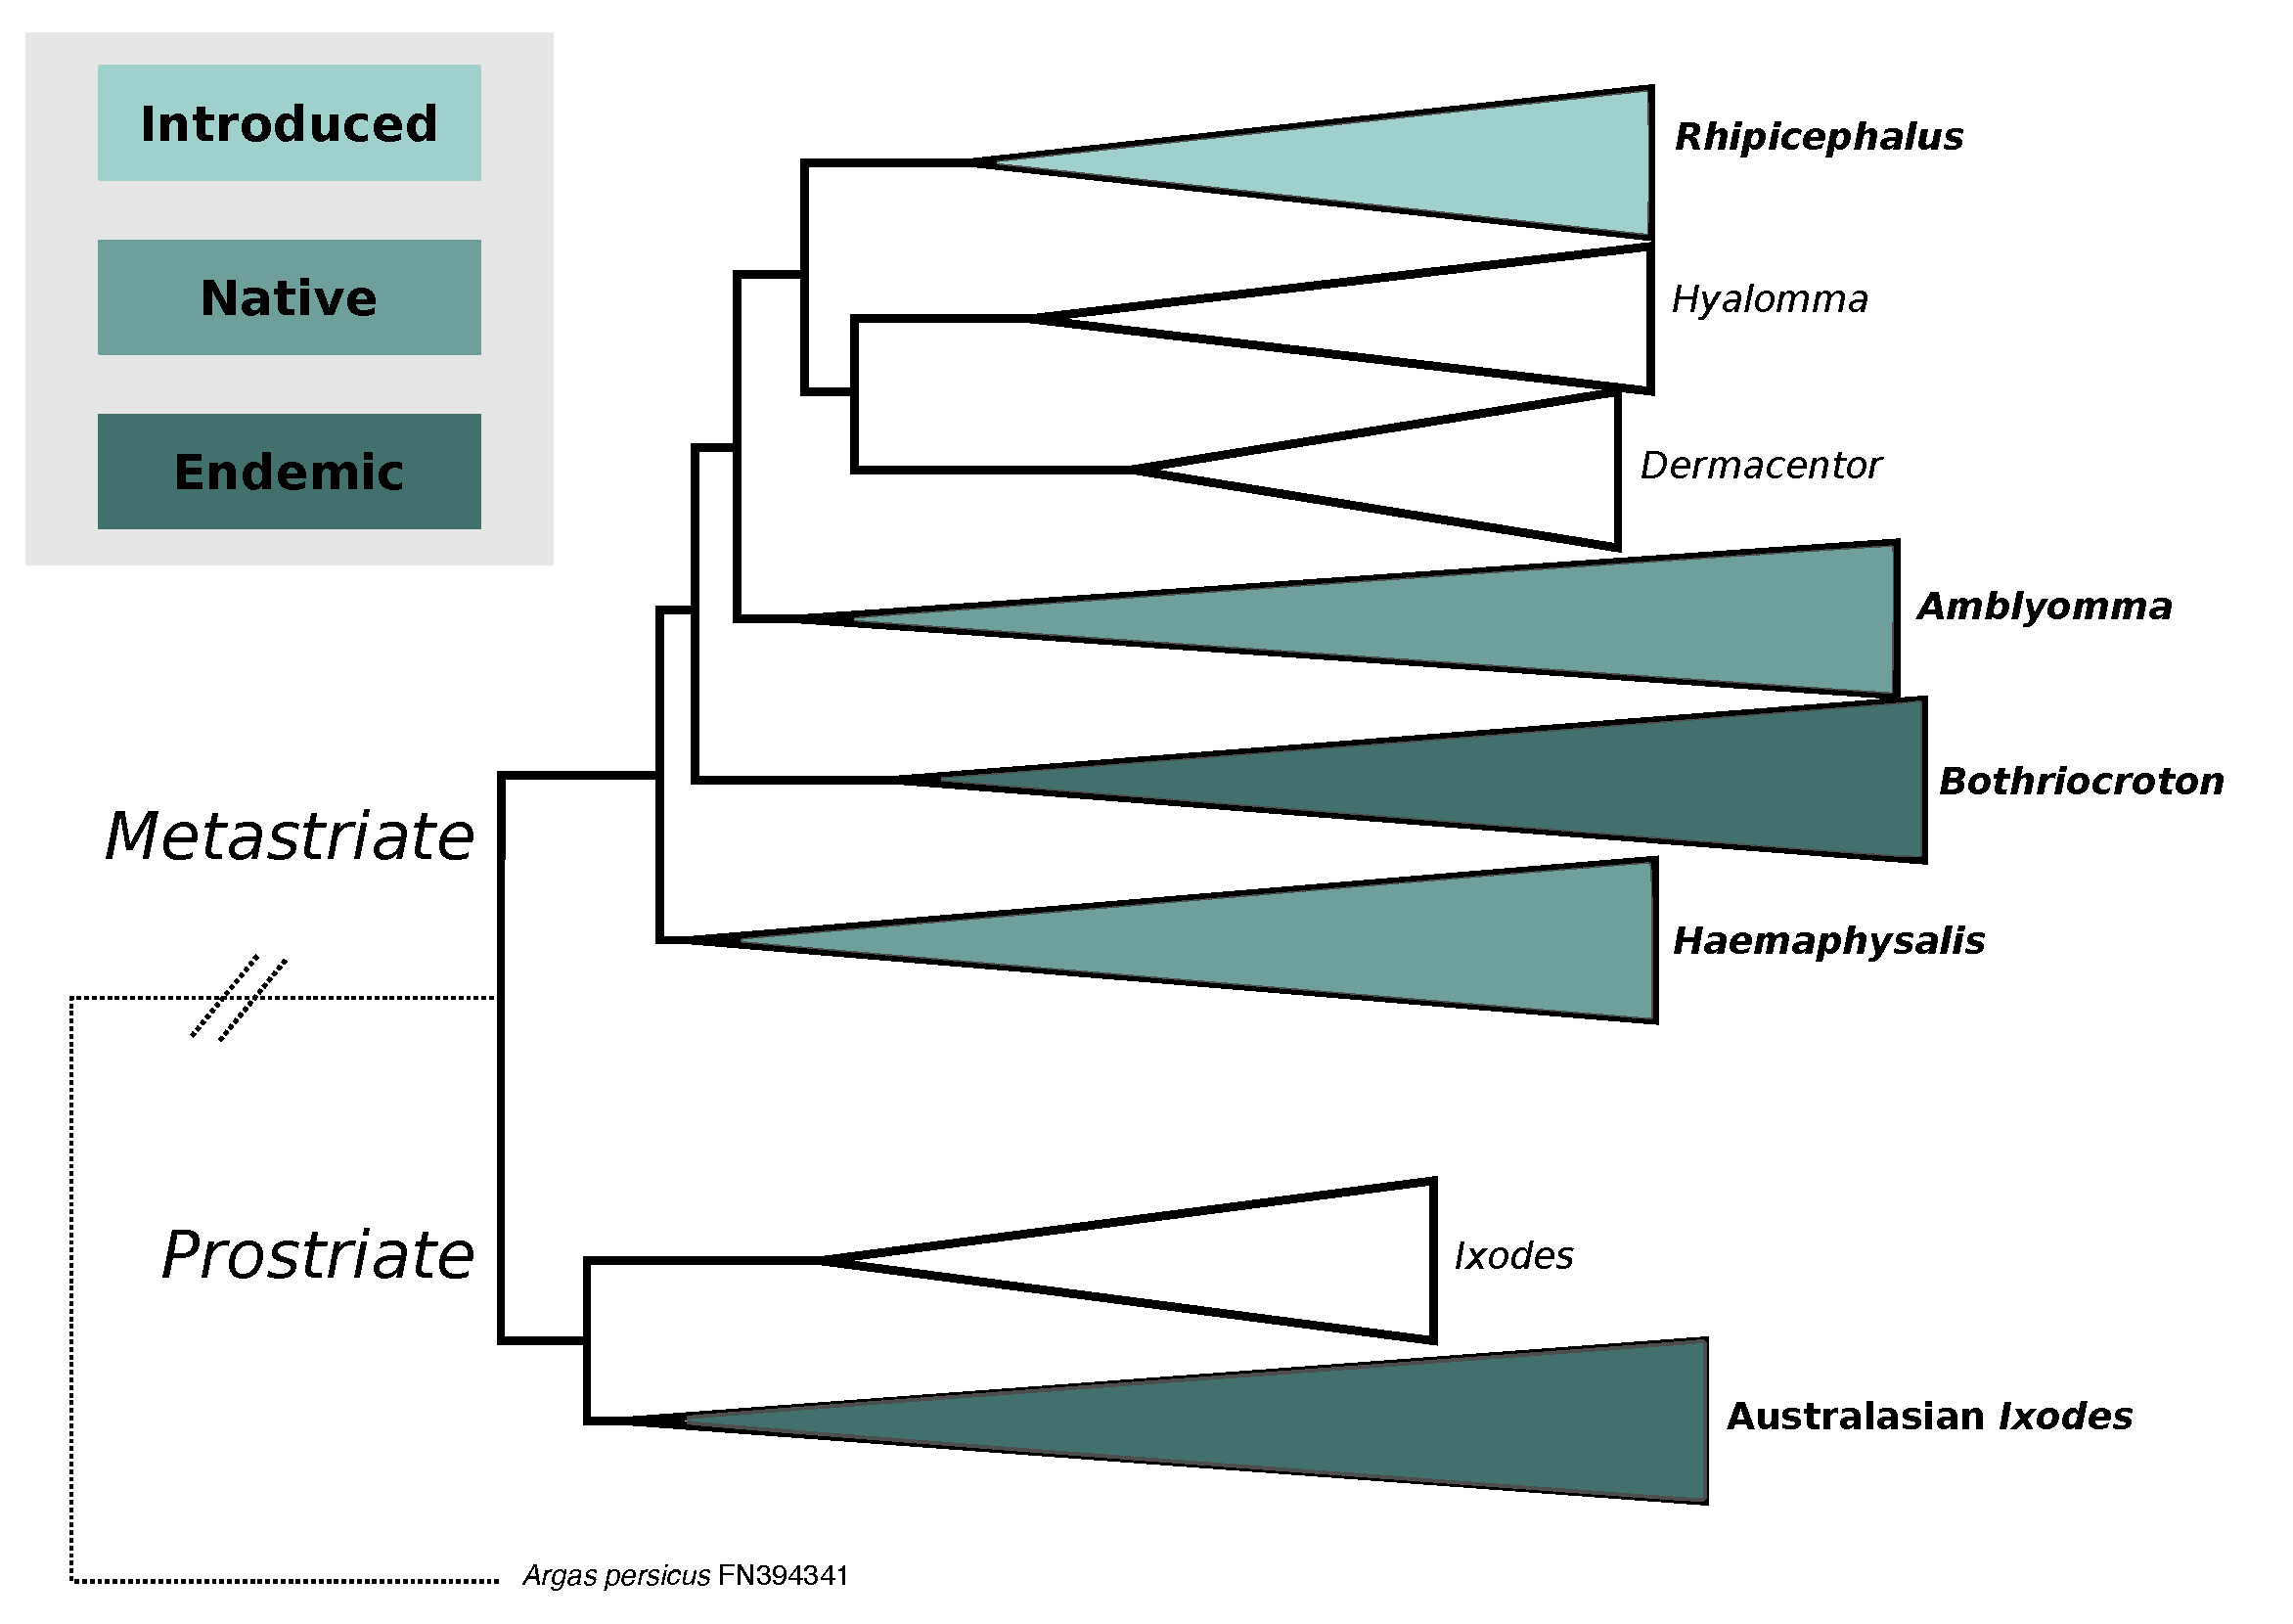
\includegraphics[width=0.95\linewidth]{figures/ms-figs/Ch1-treeixod} \caption[Phylogeny of hard tick genera (Ixodidae)]{Phylogeny of extant genera within the hard tick family (Ixodidae).}\label{fig:F1treeixod}
\end{figure}

To date Australia has 74 extant described tick species (Figure \ref{fig:F1ausixod}).
Five of these were introduced with domestic animals following European arrival in 1788: \emph{Argas persicus}, \emph{Otobius megnini}, \emph{Haemaphysalis longicornis}, \emph{Rhipicephalus sanguineus} (recently proposed as \emph{Rh. linnaei}), and \emph{Rhipicephalus australis} (\emph{Boophilus microplus)} \autocite{barkerTicksAustraliaSpecies2014}.
The first new native Australian \emph{Ixodes} tick was described in over 50 years, from woylies (\emph{Bettongia penicillata}), a critically endangered marsupial in south-west Western Australia and was named \emph{Ixodes woyliei} \autocite{ashMorphologicalMolecularDescription2017}.
The text `Australian Ticks' by Roberts \autocite*{robertsAustralianTicks1970} remains the foundation reference guide on ticks in Australia, in particular the detailed specimen descriptions and taxonomic keys used for morphological identification.
The more recent guide, `Ticks of Australia' by Barker and Walker \autocite*{barkerTicksAustraliaSpecies2014}, has provided a much needed update on the most common tick species that effect humans and animals in Australia.
As raised by Barker et al. \autocite*{barkerList70Species2014} there are a number of issues surrounding the list of recognised ticks in Australia.
Since Barker et al. \autocite*{barkerList70Species2014} there have also been a number of taxonomic changes and new information has been presented showing that the full picture of tick taxonomy in Australia is not yet complete.
In many cases host records of tick species in Australia are scarce and a large amount of time has passed since some records.
This has resulted in a number of queries surrounding the complete list of tick species present in Australia.
In some cases systematic classification remains elusive with biological data incomplete.
Issues relating to classification and/or presence of Australian ticks include:
(i) \emph{Amblyomma flavomaculatum} (yellow spotted monitor lizard tick) was listed in Roberts \autocite*{robertsAustralianSpeciesAponomma1953,robertsFurtherObservationsAustralian1964,robertsAustralianTicks1970} and referred to as \emph{Aponomma pulchrum}, which is now synonymous with \emph{Am. flavomaculatum}.
\hl{However, since these records by Roberts, there have been no positive identifications of this tick in Australia};
(ii) the distinction between \emph{Amblyomma australiense} and \emph{Amblyomma echidnae} remains unclear \autocite{guglielmoneCommentsControversialTick2009}. \emph{Amblyomma australiense} was originally described from a museum specimens of the long-beaked echidna (\emph{Zaglossus bruijnii}) in the Kimberly.
Roberts \autocite*{robertsAustralianTicks1970} leaves open the possibility that \emph{Am. echidnae} is a subspecies of \emph{Am. australiense}.
(iii) the status of \emph{Bt. tachyglossi} was resurrected by Andrews \autocite*{andrewsSystematicStatusAponomma2006}, however prior to that it was considered a synonym of \emph{Bt. hydrosauri}, therefore records prior to 2006 should be treated with caution;
(iv) records of \emph{Haempahysalis longicornis} were previously referred to as \emph{Haemaphysalis bispinosa} \autocite{robertsSystematicStudyAustralian1963}, it is now recognised that \emph{Ha. bispinosa} is a distinct species distributed across parts of Asia and early records were attributed.

Changes in tick nomenclature and taxonomy can cause disruption to ecologists, veterinarians and physicians.
In many instances changes in species names takes many years to filter through for use by the broader scientific community and for new names to be fully adopted.
For example, the reptile tick \emph{Bt. hydrosauri} (formerly \emph{Aponomma hydrosauri}) is an important vector of human disease (\emph{Rickettsia honei)}, and its changing species name can cause confusion to the public and medical professionals (e.g. \textcite{stenosAponommaHydrosauriReptileassociated2003}).
Additionally the lack of accurate keys and morphological descriptions is particularly challenging in these instances.
\hl{In the case of tick-borne diseases. accurate tick identification can greatly assist in a timely diagnosis. In areas where tick-borne disease knowledge is limited, such as Australia, accurate tick identification is of great benefit to researchers and clinicians attempting to untangle novel disease causes}.
In the case of \emph{Ix. holocyclus} and \emph{Ix. cornuatus}, only recently has sufficient keys and genetic data been published to allow the identification between these two morphologically very similar species \autocite{songPhylogeneticPhylogeographicRelationships2011,barkerTicksAustraliaSpecies2014,kwakKeysMorphologicalIdentification2017}.
\emph{Ixodes holocyclus} remains the most important vector of illness to Australians being the cause of paralysis, mammalian meat allergy, significant local reactions \hl{and} allergic responses and the vector of rickettsial diseases.
\hl{There are many suspected misidentifications of \emph{Ix. holocyclus}; for example Tasmanian devils (\emph{Sarcophilus harrisii}) in Tasmania (TAS) \autocite{vilcinsDetectionHepatozoonSpotted2009}, likely \emph{Ix. cornuatus}, and numbats (\emph{Myrmecobius fasciatus}), in Western Australia (WA) \autocite{calabyObservationsBandedAnteater1960}, likely \emph{Ix. myrmecobii}.}
More recently the Australian brown dog tick has been renamed to \emph{Rhipicephalus linnaei} \autocite{slapetaTropicalLineageBrown2021}, previously known as \emph{Rhipicephalus sanguineus} tropical lineage.
This name change is likely to create debate among taxonomist and the tick community, and therefore cause confusion for the general public.
While taxonomy is the foundation of biological science and must be corrected were appropriate, it does cause unavoidable consequences in the short term.

The unique Australian tick fauna is an important consideration in understanding the presence of tick-borne diseases, which are discussed in further detail in section three of this literature review. Tick-borne pathogens have coevolved in their vector host, and as such, the evolutionary history of Australian ticks means that it is likely that pathogens present elsewhere in the world would be different from those that have evolved with native Australian ticks.

\begin{figure}

\includegraphics[width=0.95\linewidth]{figures/ms-figs/Ch1-ausixod} \caption[Tick species (Ixodida) of Australian.]{Ticks (Ixodida) present in Australian (74 extant species).}\label{fig:F1ausixod}
\end{figure}

\hypertarget{tick-biology-and-ecology}{%
\subsection{Tick biology and ecology}\label{tick-biology-and-ecology}}

Ticks have a remarkably long life cycle compared to other vectors of infectious disease, such as mosquitoes (Culicidae) and lice (Phthiraptera).
The life cycle of wild hard ticks is often measured in years and consists of four major stages; eggs, larva, nymph and adult.
With the exemption of the egg stage, development requires a blood meal, which often involves several hours, or even days of engorgement \autocite{cuppBiologyTicks1991}.
The vast majority of hard ticks have a three-host life cycle, where each life stage feeds on a host and then detaches to spend some time in the environment before moulting to the next stage.
Adult females are able to detach and reattached multiple times to continue feeding.
\hl{In the case of generalised tick species, current literature suggests that in most cases, immature life stages (e.g.~larva and nymphs) feed on small to medium sized hosts and adult life stages feed on larger hosts \autocite{apanaskevichLifeCyclesNatural2014}}.
Although this has been shown to occur in many cases such as \emph{Ixodes ricinus} \autocite{krasnovHostCommunityStructure2007}, detailed studies on the life cycle and host dynamics of Australian ticks remains largely unknown.

Host specificity is the association between a tick and vertebrate species that is critical for the ongoing survival and reproduction of the tick \autocite{hoogstraalTickhostSpecificity1982}.
\hl{There have been suggestions that} up to 90\% of tick species are considered `host specific' \autocite{hoogstraalTickhostSpecificity1982}.
However, there has been suggestions that this finding is simply due to the incomplete sampling and reporting of tick-host records \autocite{klompenEvolutionTicks1996}.
In Australia, the primary reference for tick-host associations remains Roberts \autocite*{robertsAustralianTicks1970}, although Barker and Walker \autocite*{barkerTicksAustraliaSpecies2014} has provided an updated reference for 16 species of veterinary and medical importance.
Despite this update however, there is no single, up-to-date reference of tick-host associations.
In many cases these findings remain buried in research laboratories, special interest groups and other niches.
Since Roberts \autocite*{robertsAustralianTicks1970} publication detailed studies on the biology, ecology \hl{and} distribution of native Australian ticks have only been carried out on a handful of species most notably; \emph{Ornithodoros gurenyi} (QLD, NT, SA, WA) \autocite{doubeEcologyKangarooTick1972,doubeTwoRacesKangaroo1975}, \emph{Amblyomma triguttatum} (SA) \autocite{waudbySeasonalDensityFluctuations2007}; \emph{Bothriocroton hydrosauri} \autocite{bullDispersalAustralianReptile1978,andrewsMatingBehaviourAustralian1980,belanHostDetectionFour1991,chiltonInterspecificDifferencesMicrohabitat1993}, \emph{Ixodes cornuatus} (VIC, TAS) \autocite{jacksonGeneticVariationTicks2000,jacksonDistributionsParalysisTicks2007,songPhylogeneticPhylogeographicRelationships2011}, \emph{Ix. holocyclus} (QLD, NSW, VIC) \autocite{doubeSeasonalPatternsAbundance1979,jacksonGeneticVariationTicks2000,jacksonDistributionsParalysisTicks2007,songPhylogeneticPhylogeographicRelationships2011}, \emph{Ixodes tasmani} (NSW) \autocite{murdochEcologyCommonMarsupial2005}, \emph{Ha. bancrofti} (VIC) \autocite{laanOccuranceTickHaemaphysalis2011}.
While these studies provide a solid foundation of Australian tick biology, in many cases they are largely limited to a relatively small study site.
An experimental investigation of \emph{Ixodes hirsti} placed 1600 larvae on rats and chickens, however they found that no larvae attached to either host species, and none survived more than 24 hours \autocite{laanObservationsBiologyDistribution2011}.
The authors described hosts removing the larvae by either eating or grooming.
The conditions of the experimental animals are not described in detail, however this perhaps suggests a host specificity of \emph{Ixodes hirsti}, although the tick-host associations reviewed in the same paper show a wide range of taxa including kangaroos (\emph{Macropus} spp.), Honeyeaters (\emph{Phylidonyris} spp.), rats (\emph{Rattus} spp.), and {[}dogs (\emph{Canis lupus familiaris}){]}.\{.correction\} \autocite{laanObservationsBiologyDistribution2011}.
The life cycle of \emph{Ix. tasmani} was shown to complete within 4 months in artificial laboratory models on rats \autocite{murdochEcologyCommonMarsupial2005}, which is comparatively short compared to other ixodids \autocite{oliverBiologySystematicsTicks1989}.
The nocturnal and nidicolous questing nature of \emph{Ix. tasmani} coincides with the activity of many of its host marsupial species \autocite{murdochEcologyCommonMarsupial2005}.

\hypertarget{tick-borne-diseases-in-humans}{%
\section{Tick-borne diseases in humans}\label{tick-borne-diseases-in-humans}}

This section of the review will briefly discuss some of the major human tick-borne diseases recognised globally, with an emphasis on bacterial pathogens.
The summary provided is by no means exhaustive, it is given in the context to explain the types of microbes that have been associated with disease in humans.
The review will then reflect on human tick-borne pathogens currently documented and characterised in Australia.
Finally it will conclude by providing a summary of recent research that has been done in relation to novel microbes in Australian ticks and how they relate to potential causative agents of human disease.

This review is confined to infectious microorganisms transmitted by ticks. An in-depth and exhaustive review of each individual microbe is beyond the scope of this literature review. Instead the following is presented to provide context to microbes which are explored in more detail throughout the thesis.
In the first instance, a general introduction of tick-associated organisms are introduced within a global context focusing on zoonotic significance.
Following this, more detail is provided from an Australian context.

\hypertarget{worldwide-summary}{%
\subsection{Worldwide summary}\label{worldwide-summary}}

Ticks are responsible for transmitting the greatest variety of pathogenic microbes of any arthropod vector.
As a consequence they are important vectors of disease that affect humans, wildlife, livestock and companion animals \autocite{jongejanGlobalImportanceTicks2004}.
Incidence of human tick-borne diseases are steadily increasing, with recent reports from the Centre of Disease Control and Prevention (CDC, United States of America) describing a two-fold increase in the number of tick-borne disease cases; this accounts for 77\% of all vector-borne diseases \autocite{rosenbergVitalSignsTrends2018}.

\hypertarget{anaplasmataceae}{%
\subsubsection{\texorpdfstring{\emph{Anaplasmataceae}}{Anaplasmataceae}}\label{anaplasmataceae}}

The family \emph{Anaplasmataceae} are a group of obligate intracellular bacteria that reside in vacuoles of eukaryotic cells.
After a major taxonomic reorganisation in 2001, the phylogeny of the \emph{Anaplasmataceae} family is now well accepted and includes \emph{Ehrlichia}, \emph{Anaplasma}, \emph{Wolbachia}, \emph{Neorickettsia} and the more recently described \emph{Neoehrlichia} \autocite{rarGeneticDiversityAnaplasma2021}.
Well known human pathogens in this group include \emph{Anaplasma phagocytophilum} and \emph{Ehrlichia chaffeensis}
\emph{Anaplasmataceae} are difficult to isolate and culture, and as such molecular tools are critical in the identification of members within this family.
Conserved genes such as \emph{16S rRNA}, \emph{groEL} and \emph{gltA} (citrate synthase gene) are used to identify and classify this group of bacteria \autocite{kawaharaUltrastructurePhylogeneticAnalysis2004}.

\emph{Anaplasma phagocytophilum} is the causative agent for granulocytic anaplasmosis in humans. The first case of human granulocytic anaplasmosis (HGA) was made in the United States in 1994 \autocite{chenIdentificationGranulocytotropicEhrlichia1994}.
However, it was not until 2001 that it reflected its current name (previously named \emph{Ehrlichia phagocytophilum}) \autocite{dumlerReorganizationGeneraFamilies2001}.
\emph{Anaplasma phagocytophilum} is also responsible for tick-borne fever in ruminants, equine anaplasmosis in horses and causes severe febrile diseases in dogs and cats \autocite{rarAnaplasmaEhrlichiaCandidatus2011}.
The vast majority of HGA cases are known from the United States, most notably in the northeastern and upper mid-western regions \autocite{mmwrFinal2009Reports2010}; \hl{although present in Europe, the prevalence is significantly lower \autocite{bakkenHumanGranulocyticAnaplasmosis2015}}.
A number of \emph{A. phagocytophilum} vectors have been identified, including \emph{Ixodes scapularis} \autocite{telfordPerpetuationAgentHuman1996,hodzicAcquisitionTransmissionAgent1998}, \emph{Ixodes ricinus} \autocite{lizPCRDetectionGranulocytic2000}, \emph{Ixodes persulcatus} \autocite{eremeevaPrevalenceBacterialAgents2006}, and \emph{Ixodes ovatus} \autocite{ohashiAnaplasmaPhagocytophilumInfected2005}.
The vertebrate reservoirs of \emph{A. phagocytophilum} remain unclear due to the presence of numerous diverse strains, however animals such as white-footed mice, white-tailed deer \autocite{telfordPerpetuationAgentHuman1996,ravynIsolationEtiologicAgent2001}, dusty-footed woodrats \autocite{nicholsonDuskyFootedWoodRats1999} and chipmunks \autocite{foleyDistinctEcologicallyRelevant2009} have been highlighted as important reservoirs.

Human ehrlichiosis is most notably caused by \emph{Ehrlichia chaffeensis}.
It was first identified in the United States as causing human monocytic ehrlichiosis (HME) \autocite{andersonEhrlichiaChaffeensisNew1991}.
Since then 4,364 of confirmed HME have been reported to the CDC between 2003-2010 \autocite{mmwrFinal2009Reports2010}.
In North America the lone star tick (\emph{Amblyomma americanum}) and white-tailed deer are regarded as the most important vector and vertebrate reservoir of the bacteria \autocite{rarAnaplasmaEhrlichiaCandidatus2011}.
To date, pathogen isolation has only been confirmed in the Unites States, however molecular and serological reports of the pathogen have been made throughout the world including Venezuela \autocite{martinezEhrlichiaChaffeensisChild2008}, Latin America \autocite{gongora-biachiFirstCaseHuman1999,dacostaMoreHumanMonocytotropic2006}, South Korea \autocite{parkDetectionAntibodiesAnaplasma2003}, and Thailand \autocite{heppnerHumanEhrlichiosisThailand1997}.

Using molecular tools, reports of an \emph{Ehrlichia}-like organism were made from \emph{Ixodes ricinus} ticks in the Netherlands \autocite{schoulsDetectionIdentificationEhrlichia1999}, and from rats (\emph{Rattus norvegicus}) in China \autocite{panEhrlichialikeOrganismGene2003}.
Further studies showed there was no cross-reactivity of this organism with members of the genera \emph{Anaplasma}, \emph{Ehrlichia} or \emph{Neorickettsia}, as such it was designated to be a new genus and was formally described by \textcite{kawaharaUltrastructurePhylogeneticAnalysis2004} as \emph{Neoehrlichia mikurensis}. The first reports of \emph{N. mikurensis} infection in humans were made in 2010 and 2011 \autocite{fehrSepticemiaCausedTickborne2010,vonloewenichDetectionCandidatusNeoehrlichia2010,welinder-olssonFirstCaseHuman2010,pekovaCandidatusNeoehrlichiaMikurensis2011} and were predominately from cases where patients were immunocompromised.
Two decades after its initial discovery, the first study was published detailing the cultivation of the organism \autocite{wassCultivationCausativeAgent2019}.
Generally a rapid and full recovery is successful after treatment with antibiotics \autocite{pekovaCandidatusNeoehrlichiaMikurensis2011}.
\emph{Neoehrlichia mikurensis} has been identified from ticks around the world including Sweden \autocite{anderssonCoinfectionCandidatusNeoehrlichia2013}, Germany \autocite{dinizCandidatusNeoehrlichiaMikurensis2011}, Austria \autocite{glatzDetectionCandidatusNeoehrlichia2014}, and Hungary \autocite{hornokMolecularAnalysisIxodes2017}.
Using transmission electron microscopy, \emph{N. mikurensis} was recently identified from tick salivary glands \autocite{ondrusPutativeMorphologyNeoehrlichia2020} providing evidence for transmission route via a tick bite.

\hypertarget{borrelia}{%
\subsubsection{\texorpdfstring{\emph{Borrelia}}{Borrelia}}\label{borrelia}}

Lyme borreliosis caused by a group of spirochaete bacteria (\emph{Borrelia burgdorferi} sensu lato) is endemic to North America and Europe.
In North America the primary vector of \emph{B. burgdorferi} s. l. is \emph{Ixodes scapularis}, and major reservoir hosts are well known to include white-footed mice and white-tailed deer \autocite{halseyRoleIxodesScapularis2018}.
In Europe the main vector responsible for Lyme Borreliosis is \emph{Ixodes ricinus} \autocite{kirsteinLocalVariationsDistribution1997} with a number of vertebrates identified as reservoir hosts throughout the continent, most notably hedgehogs (\emph{Erinaceus europaeus}) and voles (\emph{Myodes glareolus}) \autocite{jahfariMeltingPotTickborne2017,coipanGeneticDiversityBorrelia2018,estrada-penaHighThroughputSequencing2018}.
Lyme borreliosis is typically manifested by an erythema migrans skin lesion (60-80\% of cases) \autocite{rizzoliLymeBorreliosisEurope2011}, and known to develop into arthritis or various skin disorders \autocite{stanekLymeBorreliosis2012}.
Additional early symptoms may include fever, headaches, fatigue, and body aches and pains \autocite{rizzoliLymeBorreliosisEurope2011,clarkLymeBorreliosisHuman2013}.
\hl{The development of neurological symptoms is another possible consequence of infection, and is known as Lyme neuroborreliosis, it has been documented in both North America and Europe \autocite{clarkLymeBorreliosisHuman2013,strleComparisonFindingsPatients2006}.}
A distinct, separate clade of \emph{Borrelia} known as the relapsing fever (RF) group, are a cause of significant disease, and can be transmitted by argasid and ixodid ticks, and the human body louse \autocite{lopezTickBorneRelapsingFever2016}.
Acute symptoms of relapsing fever in humans are generally non-specific (e.g.~fever, headache and nausea); however the disease is characterize by a unique cyclic nature, where acute episodes lasting a few days are followed by afebrile periods \autocite{dworkinTickborneRelapsingFever2008}.
\hl{In addition to the groups of Lyme borreliosis and relapsing fever \emph{Borrelia}, there are a number of phylogenetically distinct genotypes which appear to be more host specific; these include `\emph{Candidatus} Borrelia mahuryensis' from avian ticks \autocite{munoz-lealCandidatusBorreliaIbitipoquensis2020}, `\emph{Candidatus} Borrelia tachyglossi' from echidna ticks \autocite{lohMolecularCharacterizationCandidatus2017} and \emph{Borrelia turcica} from reptiles ticks \autocite{gunerBorreliaTurcicaSp2004}}.

\hypertarget{coxiella}{%
\subsubsection{\texorpdfstring{\emph{Coxiella}}{Coxiella}}\label{coxiella}}

An obligate intracellular bacteria, \emph{Coxiella} has been isolated from a wide range of animals, and environmental samples throughout the world.
\emph{Coxiella burnetii} is the causative agent of Q fever that can cause disease in both humans and animals (mainly associated with livestock) \autocite{gonzalez-barrioCoxiellaBurnetiiWild2018}.
First discovered in Australia in 1935 after a cluster of abattoir workers became ill \autocite{derrickFEVERNEWFEVER1937} the causative agent of the disease was not know, and the term Q fever was adapted meaning ``query''.
Since then it has been described in multiple countries, with incidences of human infection usually associated with direct livestock contact.
Despite the wide spread prevalence and economic impacts on the agriculture industry, the natural history of \emph{C. burnetii} is not well understood.
Q fever is usually acquired via inhalation route during close contact with infected animal material.
It has now been well established that ticks can become reservoirs and potential vectors of \emph{C. burnetii} \autocite{arricau-bouveryFeverEmergingReemerging2005}, however the significance of ticks in transmission of the disease to humans is not yet fully understood.
\hl{Many other members of the \emph{Coxiella} genus have been identified from ticks, and it is hypothesized that these species are mutualistic endosymbionts, which may provide nutritional advantages to the tick \autocite{kobayashiMolecularDetectionGenotyping2021}.}

\hypertarget{rickettsia}{%
\subsubsection{\texorpdfstring{\emph{Rickettsia}}{Rickettsia}}\label{rickettsia}}

The genus \emph{Rickettsia} (Rickettsiaceae) is a group of obligate intracellular bacteria, that are among some of the oldest known vector-borne pathogens.
Members of the genus \emph{Rickettsia} can broadly be classified into (i) spotted fever group (SFG), (ii) typhus group (iii) \emph{Rickettsia bellii} (ancestral) group and the (iv) \emph{Rickettsia canadensis} group \autocite{merhjRickettsialEvolutionLight2010}.
The SFG is the most notable group of tick-borne disease, mainly transmitted by Ixodidae ticks \autocite{parolaUpdateTickBorneRickettsioses2013}.
Rocky-mountain spotted fever (RMSF), caused by \emph{Rickettsia rickettsii} is the most well understood and studied SFG \emph{Rickettsia}.
Important vectors of \emph{R. rickettsii} in North and Central America include the Rocky Mountain wood tick (\emph{Dermacentor andersoni}), the American dog tick (\emph{Dermacentor variabilis}), the Cayenne tick (\emph{Amblyomma cajennense}) and the brown dog tick (\emph{Rhipicephalus sanguineus)} \autocite{dantas-torresRockyMountainSpotted2007,lopez-perezDiversityRickettsiaeDomestic2021}.
Although domestic dogs and wild mammals have been known to harbor the bacteria, the role of these reservoir hosts remains unclear.
Dogs have been implicated as the main reservoir for \emph{Rickettsia felis}, a flea-borne spotted-fever \emph{Rickettsia} most common in companion animals \autocite{ng-nguyenDomesticDogsAre2020}.
In other cases, small mammals, mainly rodents, are implicated in the life cycle of many \emph{Rickettsia} species \autocite{tomassoneNeglectedAspectsTickborne2018,parisBriefHistoryMajor2020}

\hypertarget{viruses}{%
\subsubsection{Viruses}\label{viruses}}

\hl{At least 38 tick-transmitted viruses have been identified, with many more unclassified species \autocite{labudaTickborneViruses2004}. With only one exception (African swine fever virus, family \emph{Asfarviridae}) all tick-borne viruses recognised belong the RNA virus families (\emph{Reoviridae}, \emph{Rhabdoviridae}, \emph{Orthomyxoviridae}, \emph{Bunyaviridae} and \emph{Flaviviridae}) \autocite{labudaTickborneViruses2004}}.
Tick-borne flaviviruses represent some of the most medically important arboviruses around the world.
Tick-borne encephalitis (TBE) (\emph{Flaviviridae}: \emph{Flavivirus}) is a growing public health issue in parts of Europe and Asia and highlights the complexity of the dynamics involved in tick-borne diseases \autocite{gritsunTickborneEncephalitis2003}.
Natural vectors of the disease involved in transmission of the virus to humans mainly include, \emph{Ixodes ricinus} and \emph{Ixodes persulcatus} \autocite{labudaTickborneViruses2004,sussTickborneEncephalitis20102011}.
The virus has also been identified in field collected \emph{Ixodes hexagonus} and studies have demonstrated that \emph{Ixodes arboricola}, \emph{Haemaphysalis concinna}, \emph{Haemaphysalis inermis} and \hl{\emph{Haemaphysalis punctata}} are also competent vectors \autocite{gresikovaTickborneEncephalitis1998}.
Vertebrate hosts involved in the maintenance of TBE include voles (\emph{M. arvalis}) and a variety of rodent species (\emph{Apodemus} spp., \emph{Microtus} spp., and \emph{Myodes} spp.) \autocite{achaziRodentsSentinelsPrevalence2011}.

\hypertarget{eukaryotes}{%
\subsubsection{Eukaryotes}\label{eukaryotes}}

Compared to bacteria, the diversity of eukaryote organisms responsible for causing tick-borne disease is much more limited \autocite{tokarzDiscoverySurveillanceTickBorne2021}.
Ticks have also been associated in the transmission and life of a diverse range of organisms such as protozoa, fungi and nematodes.

Piroplasms are a group of single-celled, intracellular parasites that belong to the Apicomplexa phylum.
Characterised by two main genera, \emph{Babesia} and \emph{Theileria}, they are the primary agents of eukaryote tick-borne diseases in vertebrates.
Human babesiosis is a well-known infectious disease, recognised as an emerging public health issue in many parts of the world.
\hl{There are over 100 species of \emph{Babesia} (Apicomplexa: Piroplasmida) worldwide which have been identified in a wide range of wildlife and domestic animals \autocite{kumarGlobalEmergenceHuman2021}. Six species of the \emph{Babesia} are recognised as capable of infection humans. In North America human babesiosis is most commonly attributed with \emph{Babesia microti}, followed by \emph{Babesia duncani}. While there has been evidence to show presence of human babesiosis in latin American countries, the true causative agents have not been as extensively studied \autocite{kumarGlobalEmergenceHuman2021}. In Europe \emph{Babesia divergens} is the main cause of human babesiosis followed by \emph{Babesia venatorum}, only a small number of cases have been attributed to \emph{B. microti} and \emph{Babesia crassa}-like agent \autocite{hildebrandtHumanBabesiosisEurope2021,vannierHumanBabesiosis2012}. Cases of babesiosis have been reported from several Asian countries with reports including \emph{Babesia crassa}-like agents, \emph{B. divergens}, \emph{B. microti}, \emph{B. venatorum}, and \emph{Babesia} spp. KO1 \autocite{kumarGlobalEmergenceHuman2021}.}
\emph{Ixodes scapularis} is the primary vector of \emph{B. microti} to humans, with most cases reportedly \hl{vectored} by nymph ticks during late spring--early summer period \autocite{spielmanEcologyIxodesDamminiborne1985,swansonCoinfectionsAcquiredIxodes2006}.
The primary vertebrate hosts identified in the transmission of the disease is the white-footed mouse (\emph{Peromyscus leucopus}) \autocite{spielmanEcologyIxodesDamminiborne1985}.
Manifestations of babesiosis are diverse, and can range from asymptomatic to debilitating illness that can lead to death.
Most commonly patients experience fever, fatigue, chills and headaches, with symptoms appearing gradually 1--4 weeks after tick bite \autocite{vannierHumanBabesiosis2008}.

The genus \emph{Theileria} is distinguished from \emph{Babesia} by the presence of stages outside the red blood cell.
There are a number of species that infect and cause disease in animals, particularly ruminants, equids, rodents, and foxes \autocite{almazanBabesiosisTheileriosisNorth2022}.
Additionally, \emph{Theileria} species have been described circulating in populations of wildlife and ticks worldwide \autocite{mansReviewTheileriaDiagnostics2015,wattsTheileriaOrientalisReview2016}.
To date, there have been no reported cases of \emph{Theileria} infecting people.

Trypanosomes are a group of flagellated protozoa that belong to phylum Euglenozoa.
Members of the genera \emph{Leishmania} and \emph{Trypanosoma} are known parasites of humans and animals and are widely distributed.
Species that can cause severe human disease include \emph{Trypanosoma cruzi}, responsible for Chagas disease in South and Central America, \hl{\emph{Trypanosoma brucei gambiense} and \emph{Trypanosoma brucei rhodesiense}} which cause human African trypanosomiasis (HAT) (also known as sleeping sickness) and \hl{\emph{Leishmania donovani}} capable of causing cutaneous leishmaniasis \autocite{kauferReviewSystematicsSpecies2020}.
Although blood-sucking insects (class Insecta) are responsible for the majority of zoonotic transmission of trypanosomes, there is growing evidence to support that ticks \hl{may be} involved in the life-cycle of these protozoans \autocite{morzariaTransmissionTrypanosomaSp1986,thekisoeTrypanosomeSpeciesIsolated2007}.

Filarial nematodes have been described from a number of tick species worldwide.
Genetic characterisation has shown that similar species of filarial nematodes have recently been described from two widespread ticks in North America.
Separate genetic analysis showed that closely related \emph{Monanema}-like filarial nematodes were identified from \emph{Amblyomma americanum} \autocite{henningDiscoveryFilarialNematode2016} and \emph{Ixodes scapularis} \autocite{tokarzCharacterizationMonanemaNematode2020}.
\hl{However, there is currently no evidence to suggest that these tick-associated nematodes are common causes of human disease \autocite{tokarzCharacterizationMonanemaNematode2020}.}

\hypertarget{infectious-human-tick-borne-pathogens-in-australia}{%
\subsection{Infectious human tick-borne pathogens in Australia}\label{infectious-human-tick-borne-pathogens-in-australia}}

In comparison to the Northern Hemisphere, relatively few zoonotic tick-borne pathogens are recognised in Australia \autocite{madison-antenucciEmergingTickBorneDiseases2020,rochlinEmergingTickbornePathogens2020}.
Queensland Tick Typhus (QTT) was first identified \hl{during World War II from} soldiers training in Queensland.
After a tick bite, individuals developed an eschar, fever and vesicular rash \autocite{andrewTickTyphusNorth1946}.
\hl{Although initial reports put it in the spotted fever group, the causative agent, \emph{Rickettsia australis} was later shown to be genetically different \autocite{stenosRickettsialOutermembraneProtein2000}}.
Early experimental work showed that \emph{Ix. holocyclus} and \emph{Ix. tasmani} were vectors of the bacteria \autocite{campbellRickettsiosesAustraliaIsolation1974}.
Since its discovery it has been identified along the east coast of Australia \autocite{campbellQueenslandTickTyphus1979,wilsonQueenslandTickTyphus2013,fergieQueenslandTickTyphus2017} (Table \ref{tab:T1ausTBD}).
A recent study using real-time PCR identified that \emph{R. australis} was present in 15.4\% (23/149) \hl{of} \emph{Ix. holocyclus} in north-east New South Wales \autocite{gravesIxodesHolocyclusTicktransmitted2016}.

A spotted-fever-like illness was identified from a cluster of 26 patients from Flinders Island, Tasmania, a small community with a population of about 1000 \autocite{stewartFlindersIslandSpotted1991}.
A serological investigation found that while 46\% of patients were positive for the detection of \emph{Rickettsia australis}, evidence suggested the aetiological agent was different \autocite{gravesSpottedFeverGroup1993}.
It was later confirmed that patients were infected with \emph{Rickettsia honei}, a pathogen originally isolated in Thailand \autocite{gravesRickettsiaHonei2003}.
An investigation into the tick reservoir on the Island found that 63\% of the reptile-associated tick \emph{Bothriocroton hydrosauri} were positive for \emph{R. honei} \autocite{stenosAponommaHydrosauriReptileassociated2003} (Table \ref{tab:T1ausTBD}).
Human infection of Q Fever, caused by the bacteria \emph{Coxiella burnetii}, is usually acquired by inhalation of infectious aerosols from vertebrate hosts such as sheep, cattle and domestic pets.
\emph{Coxiella burnetii} has been identified in a number of ticks, including the human biting species \emph{Ix. holocyclus} \autocite{gravesIxodesHolocyclusTicktransmitted2016} and \emph{Am. triguttatum} \autocite{popeCoxiellaBurnetiKangaroos1960,cooperSerologicalEvidenceCoxiella2012} (Table \ref{tab:T1ausTBD}); however there is just a single published report of tick-borne Q fever in Australia (thought to be transmitted by \emph{Am. triguttatum}) \autocite{beamanPericarditisAssociatedTickborne1989}.

\newpage

\textbf{Taxa of interest}

\hl{This next section will review recent research on tick-associated organisms that are related to taxa known to cause disease globally (i.e.~family level relatedness) and `endosymbiont' organisms from Australian ticks}.
The list of possible microbes is extensive and therefore this review will focus mainly on microbes that have been identified from ticks.
Additionally as recent research has highlighted that microbes may have a broader vector range than previously thought (e.g.~\emph{Bartonella}), where relevant this review will include other vector-related microbes.

\begin{table}

\caption[Australian human tick-borne diseases.]{\label{tab:T1ausTBD}Currently recognised Australian human tick-borne diseases.}
\centering
\fontsize{8.5}{10.5}\selectfont
\begin{tabular}[t]{l>{}l>{}l}
\toprule
Disease & Pathogen & Tick vector\\
\midrule
Queensland tick typhus & \em{Rickettsia australis} & \em{Ixodes holocyclus, Ixodes cornuatus, Ixodes tasmani}\\
Flinders Island Spotted Fever & \em{Rickettsia honei} & \em{Ixodes tasmani, Bothriocroton hydrosauri}\\
Australian Spotted Fever & \em{Rickettsia honei marmionii} & \em{Haemaphysalis novaeguinae}\\
Q Fever & \em{Coxiella burnetii} & \em{Ixodes holocyclus, Amblyomma triguttatum}\\
\bottomrule
\end{tabular}
\end{table}

\hypertarget{anaplasmataceae-1}{%
\subsubsection{\texorpdfstring{\emph{Anaplasmataceae}}{Anaplasmataceae}}\label{anaplasmataceae-1}}

Through the recent use of molecular tools five novel species (or genotypes) of \emph{Anaplasmataceae} have been described from native Australian ticks.
Additionally, a number of organisms are known but remain to be formally described (Table \ref{tab:T1anaplasm}).

Questing \emph{Am. trigutattum} ticks were found to harbour Australia's first endemic \emph{Ehrlichia}, `\emph{Ca}. Ehrlichia occidentalis' and a novel genotype of \emph{Anaplasma bovis} Y11 \autocite{goftonDetectionPhylogeneticCharacterisation2017}.
\hl{Two species of \emph{Neoehrlichia} were recently characterised from} \emph{Ix. holocyclus} along the east coast of Australia at a prevalence of 11.25\% (44/391; 31 females, seven males and six nymphs) \autocite{goftonPhylogeneticCharacterisationTwo2016}.
The disease potential and transmission dynamics of these novel organisms remains unknown.
A study on the microbiome of ticks parasitsing bandicoots confirmed the presence of both \emph{Neoehrlichia} species and expanded the tick associations to include \emph{Ix. tasmani} \autocite{eganBacterialCommunityProfiling2020}.
The same study also expanded the range of \emph{A. bovis} Y11 to New South Wales and identified a novel \emph{Neoehrlichia} and \emph{Ehrlichia} species in ticks from quenda (\emph{Isoodon fusciventer}) in south-west Western Australia.
`\emph{Candidatus} Ehrlichia ornithorhynchi' was described from the platypus and its tick \emph{Ixodes ornithorhynchi} \autocite{goftonNovelEhrlichiaSpecies2018}.
A novel \emph{Anaplasma} and \emph{Ehrlichia} species has been identified in \emph{Bothriocroton concolor} ticks from echidna in New South Wales and Queensland \autocite{lohIdentificationCharacterisationMicroorganisms2018,eganBacterialCommunityProfiling2020}.
A novel \emph{Neoehrlichia} and \emph{Ehrlichia} were also identified from ticks (\emph{Ixodes fecialis} and \emph{Ixodes australiensis}) removed from quenda \emph{Isoodon fusciventer} \autocite{eganBacterialCommunityProfiling2020}.

\begin{table}

\caption[\textit{Anaplasmataceae} species identified from Australian ticks.]{\label{tab:T1anaplasm}\textit{Anaplasmataceae} species identified from Australian ticks using molecular methods.}
\centering
\fontsize{8}{10}\selectfont
\begin{threeparttable}
\begin{tabular}[t]{>{\raggedright\arraybackslash}p{10em}>{\raggedright\arraybackslash}p{10em}>{\raggedright\arraybackslash}p{8em}>{\raggedright\arraybackslash}p{6em}>{\raggedright\arraybackslash}p{6em}>{\raggedright\arraybackslash}p{6em}}
\toprule
Microorganism & Tick species & Vertebrate host & Identified in host & State & Reference(s)\\
\midrule
Anaplasma bovis (a) & \em{Am. triguttatum} & Questing & No & NSW, WA & Gofton et al. 2017; Egan et al. 2020a\\
Anaplasma platys (a) & \em{Rh. sanguineus} & Dog & Yes & NT, QLD, SA, WA & Brown et al. 2001; Greay 2021\\
Anaplasma sp. & \em{Bt. auruginans} & Wombat & No & VIC & Beard et al. 2021\\
Anaplasma sp. & \em{Bt. concolor} & Echidna & No & QLD, NSW & Loh 2018\\
Ehrlichia canis (b) & \em{Rh. sanguineus} & Dog & Yes & NT, SA, WA & (b)\\
‘Ca. Ehrlichia occidentalis’ & \em{Am. triguttatum} & Questing & No & SA, WA & Gofton et al. \vphantom{1} 2017\\
‘Ca. Ehrlichia ornithorhynchi’ & \em{Ix. ornithorhynchi} & Platypus & Yes & QLD, TAS & Gofton et al. 2018\\
‘Ca. Ehrlichia occidentalis’ & \em{Am. triguttatum} & Questing & No & SA, WA & Gofton et al. 2017\\
Ehrlichia sp. & \em{Ix. fecialis} & Bandicoot & No & WA & Egan et al. 2020a\\
Ehrlichia sp. & \em{Bt. concolor} & Echidna & No & QLD, NSW & Loh 2018\\
‘Ca Neoehrlichia arcana’ & \em{Ix. cornuatus, Ix. holocyclus, Ix. tasmani} & Bandicoot, cat, dog, horse, human & No & NSW, QLD & Gofton et al. 2016; Egan et al. 2020a; Greay et al. 2022\\
‘Ca. Neoehrlichia australis’ & \em{Ix. holocyclus, Ix. tasmani} & Bandicoot, cat, cattle, dog, horse, human & No & NSW, QLD & Gofton et al. 2016; Egan et al. 2020a; Greay et al. 2022\\
Neoehrlichia sp. & \em{Ix. australiensis, Ix. fecialis} & Bandicoot & No & WA & Egan et al. 2020a\\
Neoehrlichia sp. & \em{Ix. holocyclus} & Cat & No & NSW & Greay et al. 2021\\
\bottomrule
\end{tabular}
\begin{tablenotes}
\item[a] Introduced species that are now considered endemic.
\item[b] Previously considered exotic, it was first identified in May 2020. Currently listed as a nationally notifiable disease and investigations into its origin are ongoing https://www.outbreak.gov.au/current-responses-to-outbreaks/ehrlichiosis-dogs.
\end{tablenotes}
\end{threeparttable}
\end{table}

\hypertarget{borrelia-1}{%
\subsubsection{\texorpdfstring{\emph{Borrelia}}{Borrelia}}\label{borrelia-1}}

At present four species of borreliae have been identified in Australia (Table \ref{tab:T1borrelia}).
Two species were introduced \emph{Borrelia theileri} and \hl{\emph{Borrelia anserina}} with the importation of livestock.
Avian spirochaetosis is associated with disease in poultry caused by \emph{B. anserina} and is transmitted by the soft tick \emph{Argas persicus}.
Bovine spirochaetosis is caused by \emph{B. theileri} and is transmitted with the cattle tick, \emph{Rhipicephalus australis} (formerly \emph{Boophilus microplus}) \autocite{estrada-penaReinstatementRhipicephalusBoophilus2012}.
The first native Australian \emph{Borrelia} was described from long-haired rats (\emph{Rattus villosissimus}) in north-western Queensland \autocite{carleyNewSpeciesBorrella1962} and named \emph{Borrelia queenslandica}.
The authors suggested the spirochaete was transmitted by the soft kangaroo tick (\emph{Or. gurneyi}), however this was never confirmed.
To date \emph{B. queensandica} has not been isolated since and as such no molecular data is available.
A recent discovery has presented the first molecular description of a native Australian \emph{Borrelia} and brings the total number of (\emph{Borrelia}) species present in Australia to four. `\emph{Candidatus} Borrelia tachyglossi' was genetically described from echidna biting ticks \hl{\emph{Bothriocroton concolor}} \autocite{lohNovelBorreliaSpecies2016,lohMolecularCharacterizationCandidatus2017}.
A novel species of \emph{Borrelia} that falls within the \hl{reptile \emph{Borrelia} clade} has also been identified in \emph{Bothriocroton undatum} collected from the goanna in NSW \autocite{panettaReptileassociatedBorreliaSpecies2017}.

\begin{table}

\caption[\textit{Borrelia} species identified from Australia.]{\label{tab:T1borrelia}\textit{Borrelia} species identified from Australian ticks and animals.}
\centering
\fontsize{8}{10}\selectfont
\begin{tabular}[t]{>{\raggedright\arraybackslash}p{10em}>{\raggedright\arraybackslash}p{10em}>{\raggedright\arraybackslash}p{8em}>{\raggedright\arraybackslash}p{6em}>{\raggedright\arraybackslash}p{6em}>{\raggedright\arraybackslash}p{6em}}
\toprule
Microorganism & Tick species & Vertebrate host & Identified in host & State & Reference(s)\\
\midrule
\em{Borrelia anserine (a)} & \em{Ar. persicus} & Poultry & Yes & QLD, NSW & Petney et al. 2004\\
\em{Borrelia queenslandica (b)} & \em{Or. gurneyi (unconfirmed)} & Rat & Yes & QLD & Carley and Pope 1962\\
\em{‘Ca. Borrelia tachyglossi’} & \em{Bt. concolor, Ha. Humerosa} & Bandicoot, echidna & Yes & NSW, QLD & Loh et al. 2016; Egan et al. 2020a\\
\em{Borrelia theileri (a)} & \em{Rh. (Bo.) australis} & Cattle & Yes & QLD & Callow and Hoyte 1961\\
\em{Borrelia sp.} & \em{Bt. undatum} & Goanna & No & NSW & Panetta et al. 2017\\
\em{Borrelia sp.} & \em{Bt. auruginans} & Wombat & No & NSW & Beard 2021\\
\bottomrule
\multicolumn{6}{l}{\rule{0pt}{1em}\textsuperscript{a} Introduced species with the important of livestock.}\\
\multicolumn{6}{l}{\rule{0pt}{1em}\textsuperscript{b} Identification made by culture methods, isolated from rodent host - suspected tick vector listed.}\\
\end{tabular}
\end{table}

\hypertarget{coxiella-1}{%
\subsubsection{\texorpdfstring{\emph{Coxiella}}{Coxiella}}\label{coxiella-1}}

Studies on the presence of \emph{Coxiella burnetii} are particularly challenging due to the cross reactivity of serological assays and the conserved nature of the commonly used 16S rRNA gene (Table \ref{tab:T1coxiella}).
Therefore in this review I will only focus on molecular reports of \emph{Coxiella} sp. from wildlife and ticks.
Sequences that were 98--99\% similar to \emph{C. burnetii} have been identified in
\emph{Bothriocroton auruginans} from the common wombat (\emph{Vombatus ursinus}) collected from Victoria \autocite{vilcinsMolecularDetectionRickettsia2009,beardMorphologicalIdentificationTicks2021}.\\
Recent descriptions of \emph{Coxiella burnetii} from native Australian tick species (\emph{Ha. bancrofti}, and \emph{Ix. holocyclus}) and the brown dog tick (\emph{Rh. sanguineus}) are important in our understanding of the epidemiology of Q Fever in Australia \autocite{chaladaMolecularSurveyTickBorne2018}.
The positive detection of \emph{C. burnetii} in these samples however has limited reliably due to the lack of DNA sequence results from the study.
The authors also noted the presence of \emph{Coxiella}-like symbionts in \emph{Am. triguttatum}, \emph{Ix. holocyclus}, \emph{Rh. australis} and \emph{Or. capensis}, which were also not sequenced.
An investigation into the presence of \emph{Coxiella} and \emph{Coxiella}-like symbionts in Australian brown dog ticks (\emph{Rh. linnaei} syn \emph{Rh. sanguineus}) revealed the presence of a \emph{Coxiella}-like symbiont (100\% prevalence) \hl{through targeted PCR and sequencing} of the 16S rRNA gene \autocite{oskamMolecularInvestigationPresence2017}.
Therefore without sequence results from PCR assays, the true presence of \emph{Coxiella burnetii} as determined by \textcite{chaladaMolecularSurveyTickBorne2018} remains questionable.\\
\emph{Coxiella burnetii} was recently detected in kangaroo meat that was intended for companion animal consumption \autocite{shapiroMolecularDetectionCoxiella2020} using qPCR.
One recent study stated that wildlife carers may be two times more likely to be infected with \emph{C. burnetii} than the general public, however the study was hindered by a small sample size \autocite{mathewsCoxiellaBurnetiiSeroprevalence2021}

\begin{table}

\caption[\textit{Coxiella} species identified from Australian ticks.]{\label{tab:T1coxiella}Identification of \textit{Coxiella burnetii} within Australian ticks and wildlife using molecular methods. Serological tests were excluded from this summary due to the known cross-reactivity of \textit{Coxiella}-like organisms with assays.}
\centering
\fontsize{8}{10}\selectfont
\begin{tabular}[t]{>{\raggedright\arraybackslash}p{10em}>{\raggedright\arraybackslash}p{10em}>{\raggedright\arraybackslash}p{8em}>{\raggedright\arraybackslash}p{6em}>{\raggedright\arraybackslash}p{6em}>{\raggedright\arraybackslash}p{6em}}
\toprule
Microorganism & Tick species & Vertebrate host & Identified in host & State & Reference(s)\\
\midrule
\em{Coxiella burnetii} & \em{Ha. bancrofti} & Horse & No & QLD & Chalada et al. 2018\\
\em{Coxiella burnetii} & \em{Ix. holocyclus} & Kookaburra & No & QLD & Chalada et al. 2018\\
\em{Coxiella burnetii} & \em{Rh. sanguineus} & Dog & No & QLD & Chalada et al. 2018\\
\em{Coxiella burnetii (a)} & \em{Ha. humerosa} & Bandicoot & No & WA (islands) & Bennett et al. 2011\\
\em{Coxiella burnetii} & \em{Ix. holocyclus} & Bandicoot & Yes & QLD & Cooper et al. 2013\\
\em{Coxiella burnetii} & \em{Am. triguttatum} & Kangaroo & Yes & QLD & Cooper et al. 2013\\
\em{Coxiella burnetii} & \em{Bt. auruginans} & Wombat & No & VIC & Vilcins et al. 2009b; Beard et al. 2021\\
\em{Coxiella burnetii} & \em{Ix. holocyclus} & Cat & No & QLD & Greay et al. 2021\\
\bottomrule
\multicolumn{6}{l}{\rule{0pt}{1em}\textsuperscript{a} Identified in a faecal sample using molecular assay.}\\
\multicolumn{6}{l}{\rule{0pt}{1em}\textsuperscript{b} Records from Islands off Western Australia coastline.}\\
\end{tabular}
\end{table}

\hypertarget{rickettsia-1}{%
\subsubsection{\texorpdfstring{\emph{Rickettsia}}{Rickettsia}}\label{rickettsia-1}}

\textbf{Spotted fever - Flinders Island Spotted or Australian Spotted fever?}

The identification of Flinders Island Spotted Fever (\emph{R. honei}) was a significant breakthrough in the knowledge of tick-borne diseases in Australia.
However, ongoing research into the distribution of the disease, and more recently genetic information, has meant the label of ``Flinders Island'' Spotted Fever causes significant issues.
Only a few years after it was formally recognised, a new focus of \emph{Rickettsia honei} spotted fever was identified in South Australia and Tasmania \autocite{dyerNewFocusRickettsia2005,unsworthNotOnlyFlinders2005}.
Lane et al. \autocite*{laneEvidenceSpottedFeverlike2005a} identified a \emph{Rickettsia honei}-like sequence from a \emph{Haemaphysalis novaeguineae} tick.
The patient was bitten by the tick in north-east Queensland and become acutely unwell developing signs of rickettsial disease (later report by Unsworth et al. \autocite*{unsworthThreeRickettsiosesDarnley2007}).
Although molecular analysis did show similarities with \emph{R. honei} strain TT-118 (Thai tick typhus), and \emph{R. honei} (Flinders Island Spotted Fever), it was not able to fully resolve the relationships among the SFG rickettsia.
A report of seven patients exhibiting similar symptoms to Flinders Island Spotted Fever was later published \autocite{unsworthThreeRickettsiosesDarnley2007}.
A combination of serological, molecular and culture techniques were used and \emph{R. honei} subsp. marmionii was described in patients from Queensland, Tasmania and South Australia.
It again confirmed the presence of the novel genotype and subsequent illness caused by a \emph{Haemaphysalis novaeguineae} bite from Cape York Peninsula in far north Queensland.
There have been no other identification of \emph{R. honei} in a tick vector on mainland Australia.
A recent case described a negative serological result from a patient, however subsequent \hl{shotgun sequencing} of the blood showed it was positive for \emph{Rickettsia honei} \autocite{grahamDetectionSpottedFever2017}.
The initial naming of the disease as ``Flinders Island'' Spotted Fever has potentially caused havoc on the diagnosis and treatment of the disease.
Due to the non-specific acute symptoms, and at times unusual sequelae of spotted-fever, it is plausible that treating physicians may not consider FISF as a possible aetiology due to geographical restrictions.
Scientifically sound and timely case reports are fundamental to ensure information is disseminated to the medical community.
A number of case reports of a \emph{Rickettsia}-like illness have also been identified from patients in Western Australia.
Molecular screening of a punch biopsy (taken at edge of eschar) sample taken from a patient bitten by \emph{Ixodes australiensis} in Walpole, south-west Western Australia showed the presence of \emph{Rickettsia} sp. (unable to identify to species).
Using a PCR assay the whole blood was negative, however serological testing showed evidence of acute infection with SFG \emph{Rickettsia}; culture and PCR from the tick were negative \autocite{rabyNewFociSpotted2016}.
A female patient was bitten by a tick 150 km east of Esperance and DNA extracted from acute phase serum underwent PCR for the rickettsial 17kD antigen gene which generated a 429 bp sequence showed 100\% similarity to \emph{R. honei}, and 99.7\% to \emph{R. gravesii}.
It is unclear if \emph{R. honei} has a larger geographical and vector range than previously thought or if in fact this was \emph{R. gravesii} sequence showing a 1 bp mis-match to reference sequence \autocite{rabyNewFociSpotted2016}.
A serological study in Western Australia showed that those who frequented bushland had a higher risk of exposure to spotted fever group rickettsia compared to the reference population \autocite{abdadSeroepidemiologicalStudyOutdoor2014}.
In addition, there have also been a number of novel \emph{Rickettsia} species recently described from native Australian ticks (Table \ref{tab:T1rickettsia}).
Importantly many of these novel findings highlight the difficultly and ambiguity in species delimitation of the genus.\\
A novel Australian \emph{Rickettsia} was identified from the soft tick \emph{Argas dewae} from bat roosting boxes in Victoria \autocite{izzardRickettsialesRickettsialDiseases2010}.
Gene sequences from five genes (\emph{gltA}, \emph{rOmpB}, \emph{rOmpA}, \emph{rrs} and \emph{sca4}) totalling over 10 kb demonstrated that it fit the criteria for the designation of a novel species as per \textcite{fournierGeneSequenceBasedCriteria2003} and was tentatively named \emph{Rickettsia dewae}.\\
However, a recent study published by the same authors illustrates how whole genome sequence revealed that it is actually a divergent strain of \emph{Rickettsia japonica} \autocite{izzardIsolationDivergentStrain2018}.
In that same study the authors also raise important questions on the classification of \emph{Rickettsia} species as outlined in \textcite{fournierGeneSequenceBasedCriteria2003}.
With the growing trend towards whole genome sequencing it may in fact raise questions around descriptions of other \emph{Rickettsia} species.

\begin{table}

\caption[\textit{Rickettsia} species identified from Australian ticks.]{\label{tab:T1rickettsia}\textit{Rickettsia} species identified from Australian ticks using molecular methods.}
\centering
\fontsize{8}{10}\selectfont
\begin{tabular}[t]{>{\raggedright\arraybackslash}p{10em}>{\raggedright\arraybackslash}p{10em}>{\raggedright\arraybackslash}p{8em}>{\raggedright\arraybackslash}p{6em}>{\raggedright\arraybackslash}p{6em}>{\raggedright\arraybackslash}p{6em}}
\toprule
Microorganism & Tick species & Vertebrate host & Identified in host & State & Reference(s)\\
\midrule
Rickettsia australis (a) & \em{Ix. holocyclus, Ix. tasmani} & Bandicoots, reptiles & Yes & NSW, QLD, VIC & Andrew et al. 1946; Brody 1946; Pope 1955; Campbell and Domrow 1974; Campbell et al. 1979\\
Rickettsia honei (a) & \em{Bt. hydrosauri} & Reptiles & No & TAS & Graves et al. 1991; Stewart 1991; Graves and Stenos 2003;  Stenos et al. 2003; Dyer et al. 2005\\
Rickettsia honei marmionii (a) & \em{Ha. novaeguineae} & Unknown & No & QLD & Lane et al. 2005; Unsworth et al. 2007a\\
Rickettsia gravesii & \em{Am. triguttatum} & Feral pigs, horses, macropods & No & QLD, WA & Owen et al. 2006b; Li et al. 2010; Sentausa et al. 2013; Abdad et al. 2017; Chalada et al. 2018\\
Rickettsia antechini & \em{Ix. antechini} & Antechinus & Yes & WA & Owen et al. 2006a; Owen 2007\\
Rickettsia tasmanensis & \em{Ix. tasmani} & Tasmanian devil & No & TAS & Izzard 2010\\
Rickettsia massillae-like & \em{Ix. tasmani} & Tasmanian devil & No & TAS & Vilcins et al. 2009c\\
Rickettsia bellii-like & \em{Bt. concolor} & Echidna & No & VIC & Vilcins et al. 2009d\\
Rickettsia massillae-like (koala genotype) & \em{Ix. tasmani} & Koala & No & NSW, VIC & Vilcins et al. 2008\\
Rickettsia massillae-like & \em{Bt. auruginans} & Wombat & No & VIC & Vilcins et al. 2009d\\
Rickettsia tamurae-like & \em{Am. fimbriatum, Bt concolor} & Echidna, reptiles & No & NT, QLD & Vilcins et al. 2009a; Chalada et al. 2018\\
Rickettsia japonica (str. argasii) & \em{Ar. (Ca.) dewae, Ha. bancrofti} & Bats, horse & No & QLD, VIC & Parola et al. 2013; Chalada et al. 2018; Izzard et al. 2018\\
Rickettsia felis & \em{Ha. bancrofti} & Horse & No & QLD & Chalada et al. 2018\\
Rickettsia sp. ARRL2016-156 & \em{Am. Albolimbatum} & Bobtail & No & WA & Tadepalli et al. 2021\\
\bottomrule
\multicolumn{6}{l}{\rule{0pt}{1em}\textsuperscript{a} Recognised human tick-borne pathogen.}\\
\end{tabular}
\end{table}

\hypertarget{viruses-1}{%
\subsubsection{Viruses}\label{viruses-1}}

Despite the presence and pathogenicity of tick-borne viruses being well described overseas, Australia does not currently recognise the presence of an endemic tick-borne virus.
Virus-tick-vertebrate host relationships are highly specific \autocite{labudaTickborneViruses2004}.
A review of neglected arboviruses in Australia highlighted that despite a surge of research pioneered by the Commonwealth Scientific and Industrial Research Organisation (CSIRO), tick-borne virus research has largely remained undocumented \autocite{gyawaliNeglectedAustralianArboviruses2017}.
A summary of past and recent virus discoveries from Australian ticks is provided in Table \ref{tab:T1virus}.

During the 1960's and 1970's there was a strong research presence around novel tick-borne viruses in Australia led by CSIRO team.
Gadgets Gully virus was described in 1976 from \emph{Ixodes uriae} ticks at Macquarie Island \autocite{st.georgeIsolationArbovirusesIncluding1985}.
The virus was isolated by intra-cerebral inoculation of ground tick suspensions into neonatal mice, which resulted in mice developing neurological symptoms and died 5 days post infection.
Serological characterisation of the isolate demonstrated that it was an unknown flavivirus however, there has been no further research and as such the ecology, transmission dynamics and its potential to cause disease in humans remains unknown.
Saumerez Reef virus was described in 1974 from \emph{Ornithorodoros capensis} ticks collected from nests of sooty terns (\emph{Sterna fuscata}), Queensland \autocite{st.georgeIsolationSaumarezReef1977}.
Several other viral isolates were obtained from the hard tick \hl{\emph{Ix. eudyptidis}}, collected in Tasmania \autocite{st.georgeIsolationSaumarezReef1977}.
Intra-cerebral inoculation of neonatal mice caused death while intra-cerebral inoculation of weanling mice did induce antibody formation and no clinical illness.
No data on potential human infection or human illness are available.
Serological studies in silver gulls (\emph{Larus novaehollandiae}) in Tasmania showed they had an antibody seroprevalence rates of 25\%. Ticks and birds are thought to contribute to the natural transmission of Saumarez Reef virus, however, further studies are needed to elucidate the natural cycle of the virus.
Vinegar Hill virus (VINHV) is a member of the Bunyavirales order (tentative member of the genus \emph{Orthonairovirus}) and was isolated from the soft tick \emph{Argas robertsi} collected from cattle egrets \autocite{gauciGenomicCharacterisationVinegar2017}.
Avian and human sera from local residents in the Coral Sea and Great Barrier Reef was used for testing against 19 known arboviruses.
It found that antibodies were detected in 4\% of avian and human sera and included Gadget's Gully virus (flavivirus) and Murray Valley Encephalitis.
It was noted however, that a number of antibodies were restricted to sea birds only.
Novel Phlebovirus with zoonotic potential was identified from a colony of shy albatross (\emph{Thalassarche cauta}) on Albatross Island, northwest of Tasmania in the Hunter Island Group \autocite{wangNovelPhlebovirusZoonotic2014}.
Both ticks (\emph{Ixodes eudyptidis}) and serum samples were collected, and sequences were obtaining via RNAseq using the 454 platform, however subsequent testing by ELISA or qPCR was unsuccessful.

A unique iflavivirus has recently been identified from \emph{Ix. holocyclus} in Queensland and New South Wales \autocite{obrienDiscoveryNovelIflavirus2018}.
Designed \emph{Ix. holocyclus} iflavirus (IhIV), it represents the first virus sequence identified in \emph{Ix. holocyclus} ticks.
Members of the \emph{Iflaviridae} family are considered `arthropod-only' viruses, and to date have not been implicated in human disease.
More recently metatranscriptomic applications have characterised a number of novel viral sequences.
Using this approach 19 novel RNA viruses were characterised which included members of the \emph{Flaviviridae} and \emph{Reoviridae} families \autocite{harveyExtensiveDiversityRNA2019}.
Members of these viral families include known human pathogens described in the northern hemisphere such as tick-borne encephalitis virus and Powassan virus (both belong to genus \emph{Flavivirus}) and Colorado tick fever virus (genus \emph{Coltivirus}).
Their isolation in the common human biting tick \emph{Ix. holocyclus} makes them important candidates for future research into possible links to cases of human disease.

\begingroup\fontsize{8}{10}\selectfont

\begin{longtable}[t]{>{\raggedright\arraybackslash}p{10em}>{\raggedright\arraybackslash}p{10em}>{\raggedright\arraybackslash}p{8em}>{\raggedright\arraybackslash}p{6em}>{\raggedright\arraybackslash}p{6em}>{\raggedright\arraybackslash}p{6em}}
\caption[Viruses identified from Australian ticks.]{\label{tab:T1virus}Viruses identified from Australian ticks using molecular and culture based methods. Name of virus and genus or family in parentheses.}\\
\toprule
Microorganism & Tick species & Vertebrate host & Identified in host & State & Reference(s)\\
\midrule
\endfirsthead
\caption[]{\label{tab:T1virus}Viruses identified from Australian ticks using molecular and culture based methods. Name of virus and genus or family in parentheses. \textit{(continued)}}\\
\toprule
Microorganism & Tick species & Vertebrate host & Identified in host & State & Reference(s)\\
\midrule
\endhead

\endfoot
\bottomrule
\multicolumn{6}{l}{\rule{0pt}{1em}\textsuperscript{a} Antibodies identified from host blood samples.}\\
\multicolumn{6}{l}{\rule{0pt}{1em}\textsuperscript{b} Records from Macquarie Island off Tasmania coastline.}\\
\multicolumn{6}{l}{\rule{0pt}{1em}\textsuperscript{c} Records from Heron Island off Queensland coastline.}\\
\multicolumn{6}{l}{\rule{0pt}{1em}\textsuperscript{d} Records from Hunter Island Group off Tasmania coastline.}\\
\multicolumn{6}{l}{\rule{0pt}{1em}\textsuperscript{e} Records from Diamond Island off Tasmania coastline.}\\
\endlastfoot
\em{Nugget virus (Orbivirus)} & \em{Ix. uriae} & Seabirds & No & TAS (b) & Doherty et al. 1975\\
\em{Taggert virus (Orthonairovirus)} & \em{Ix. uriae} & Seabirds & No & TAS (b) & Doherty et al. 1975\\
\em{Lake Clarendon virus (Reoviridae)} & \em{Ar. robertsi} & Cattle egrets & (a) & QLD & St. George et al. 1984\\
\em{Precarious Point virus (Phlebovirus)} & \em{Ix. uriae} & Seabirds & No & TAS (b) & St. George et al. 1985\\
\em{Upolu virus (Thogotovirus)} & \em{Or. capensis} & Seabirds & No & QLD & Doherty et al. 1968; Briese et al. 2014\\
\em{Gadgets Gully virus (Flavivirus)} & \em{Ix. uriae} & Seabirds & No & TAS (b) & St. George, 1991\\
\em{Saumarez Reef virus (Flavivirus)} & \em{Or. capensis, Ix. eudyptidis} & Seabirds & No & QLD, TAS & St. George et al. 1977\\
\em{Johnston Atoll virus (Quarjavirus)} & \em{Or. capensis} & Seabirds & No & QLD (c) & Doherty et al. 1968\\
\em{Vinegar Hills virus (Orthonairovirus)} & \em{Ar. robertsi} & Cattle egrets & No & QLD & St. George, 2011; Gauci et al. 2017\\
\em{Hunter Island Group virus (syn. Albatross Island virus) (Phlebovirus)} & \em{Ix. eudyptidis} & Seabirds & No & TAS (d) & Wang et al. 2014; Gauci et al. 2015\\
\em{Catch-me-Cave virus (Phlebovirus)} & \em{Ix. uriae} & Seabirds & No & TAS (b) & Major et al. 2009\\
\em{Finch Creek virus  (Orthonairovirus)} & \em{Ix. uriae} & Seabirds & No & TAS (b) & Major et al. 2009\\
\em{Sandy Bay virus (Orbivirus)} & \em{Ix. uriae} & Seabirds & No & TAS (b) & Major et al. 2009\\
\em{Little Diamond Island virus group (Uknown)} & \em{Ix. kohlsi} & Seabirds & No & TAS (e) & Major et al. 2009\\
\em{Iflavivirus (iFlaviviridae)} & \em{Ix. holocyclus} & Mammals & No & NSW, QLD & O'Brien et al. 2018\\
\em{Manly virus (Rhabdoviridae)} & \em{Am. moreliae} & Blue-tongue & No & NSW & Harvey et al. 2019\\
\em{Fairlight virus (Mononegavirales)} & \em{Am. moreliae} & Blue-tongue & No & NSW & Harvey et al. 2019\\
\em{Cannae Point virus (Chuviridae)} & \em{Am. moreliae} & Blue-tongue & No & NSW & Harvey et al. 2019\\
\em{Store Beach virus (Luteo-like virus)} & \em{Am. moreliae} & Blue-tongue & No & NSW & Harvey et al. 2019\\
\em{Quarantine Head virus (Mononegavirales)} & \em{Am. moreliae} & Blue-tongue & No & NSW & Harvey et al. 2019\\
\em{North Shore virus (Partitiviridae)} & \em{Ix. holocyclus} & Bandicoot, human, questing & No & NSW & Harvey et al. 2019\\
\em{Blue Fish Point virus (Luteo-like virus)} & \em{Ix. holocyclus} & Bandicoot, black rat & No & NSW & Harvey et al. 2019\\
\em{Shelly Headland virus (Reoviridae)} & \em{Ix. holocyclus} & Bandicoot & No & NSW & Harvey et al. 2019\\
\em{Jump Rock virus (Picornaviridae)} & \em{Ix. holocyclus} & Bandicoot & No & NSW & Harvey et al. 2019\\
\em{Ingleside virus (Virgaviridae)} & \em{Ix. holocyclus} & Bandicoot, questing & No & NSW & Harvey et al. 2019\\
\em{Collins Beach virus (Flaviviridae)} & \em{Ix. holocyclus} & Bandicoot & No & NSW & Harvey et al. 2019\\
\em{Fairfax Lookout virus (Flaviviridae)} & \em{Ix. trichosuri} & Bandicoot, bush rat & No & NSW & Harvey et al. 2019\\
\em{Timbillica virus (Phenuiviridae)} & \em{Ix. holocyclus} & Bandicoot & No & NSW & Harvey et al. 2019\\
\em{Genoa virus (Chuviridae)} & \em{Ix. holocyclus} & Bandicoot & No & NSW & Harvey et al. 2019\\
\em{Nadgee virus (Narnaviridae)} & \em{Ix. holocyclus} & Bandicoot & No & NSW & Harvey et al. 2019\\
\em{Wangarabell virus (Narnaviridae)} & \em{Ix. holocyclus} & Bandicoot & No & NSW & Harvey et al. 2019\\
\em{Yambulla virus (Narnaviridae)} & \em{Ix. holocyclus} & Bandicoot & No & NSW & Harvey et al. 2019\\
\em{Old Quarry Swamp virus (Orthomyxoviridae)} & \em{Ix. holocyclus} & Bandicoot, black rat & No & NSW & Harvey et al. 2019\\
\em{Shelly Beach virus (Reoviridae)} & \em{Ix. holocyclus} & Bandicoot, black rat & No & NSW & Harvey et al. 2019\\*
\end{longtable}
\endgroup{}

\hypertarget{eukaryotes-1}{%
\subsubsection{Eukaryotes}\label{eukaryotes-1}}

Eukaryote organisms reviewed here were chosen based on their relationship with known agents responsible for tick-borne diseases globally.
Taxa included within this section include piroplasms (e.g.~\emph{Babesia} and \emph{Theileria}), \emph{Hepatozoon}, and \emph{Trypanosoma}.
These organisms can broadly be classified as haemoprotozoa.
In Australia there is currently no recognised human eukaryote tick-borne pathogens.
So far studies have failed to provide evidence for agents of human tick-borne diseases that have been described in the northern hemisphere to be present in Australia.

Due to the recognised issues associated with morphological identification of haemoprotozoa \autocite{zhuLooksCanDeceive2009,lackPhylogenyEvolutionPiroplasmida2012,kostygovEuglenozoaTaxonomyDiversity2021} this review will focus on molecular identifications of eukaryotes from Australian ticks.
A summary of selected eukaryote organisms that have been identified from Australian ticks are available in Table \ref{tab:T1eukaryotes}.

\begingroup\fontsize{8}{10}\selectfont

\begin{longtable}[t]{>{\raggedright\arraybackslash}p{10em}>{\raggedright\arraybackslash}p{10em}>{\raggedright\arraybackslash}p{8em}>{\raggedright\arraybackslash}p{6em}>{\raggedright\arraybackslash}p{6em}>{\raggedright\arraybackslash}p{6em}}
\caption[Eukaryotes identified from Australian ticks.]{\label{tab:T1eukaryotes}A selection of eukaryotes identified from Australian ticks using molecular based methods. Eukaryotes groups presented here represent organisms related to taxa associated with tick-borne diseases globally.}\\
\toprule
Microorganism & Tick species & Vertebrate host & Identified in host & State & Reference(s)\\
\midrule
\endfirsthead
\caption[]{\label{tab:T1eukaryotes}A selection of eukaryotes identified from Australian ticks using molecular based methods. Eukaryotes groups presented here represent organisms related to taxa associated with tick-borne diseases globally. \textit{(continued)}}\\
\toprule
Microorganism & Tick species & Vertebrate host & Identified in host & State & Reference(s)\\
\midrule
\endhead

\endfoot
\bottomrule
\multicolumn{6}{l}{\rule{0pt}{1em}\textsuperscript{a} Imported species that are now considered endemic.}\\
\multicolumn{6}{l}{\rule{0pt}{1em}\textsuperscript{b} Previously considered an exotic species to Australia, first identification made in 2018.}\\
\multicolumn{6}{l}{\rule{0pt}{1em}\textsuperscript{c} Retrospective sequence analysis showed that sequences are more similar to the genus Hemolivia.}\\
\endlastfoot
\em{Babesia bigemina (a)} & \em{Rh. (Bo.) australis} & Cattle & Yes & NSW, QLD, WA & Angus 1996; Jonsson et al. 2008\\
\em{Babesia bovis (a)} & \em{Rh. (Bo.) australis} & Cattle & Yes & NSW, QLD, WA & Angus 1996; Jonsson et al. 2008\\
\em{Babesia canis vogeli (a)} & \em{Rh. sanguineus} & Dog & Yes/No & NT, Torres Strait & Jefferies et al. 2003; Greay et al. 2018b\\
\em{Babesia lohae} & \em{Ix. holocyclus} & Cat & No & QLD & Greay et al. 2018b\\
\em{Babesia sp. (lohae-like)} & \em{Ix. holocyclus, Ix. tasmani} & Brushtail possum & No & NSW, QLD & Loh et al. 2018a\\
\em{Babesia sp. (lohae-like)} & \em{Ixodes sp., Ix. holocyclus} & Eastern grey kangaroo, red-necked wallaby & No & NSW, QLD & Storey-Lewis 2018\\
\em{Babesia mackerrasorum} & \em{Haemaphysalis sp.} & Horse & No & NSW & Greay et al. 2018b\\
\em{Babesia sp.} & \em{Ixodes sp., Ix. holocyclus, Ha. Petrogalis} & Red-necked wallaby, unknown & No & NSW, QLD & Storey-Lewis 2018\\
\em{Babesia sp.} & \em{Haemaphysalis sp., Ha. petrogalis} & Eastern grey kangaroo, red-necked wallaby & No & NSW, QLD & Storey-Lewis 2018\\
\em{Theileria apogeana} & \em{Ix. tasmani} & Dog & No & TAS & Greay et al. 2018b\\
\em{Theileria fuliginosa-like} & \em{Ix. australiensis} & Western grey kangaroo & No & WA & Loh et al. 2018b\\
\em{Theileria orientalis (a)} & \em{Ha. longicornis, Ha. bancrofti} & Cattle, dog, questing, red fox & No & NSW & Hammer et al. 2015; Greay et al. 2018b; Loh et al. 2018a; Marendy et al. 2019; Emery et al. 2021; Lakew et al. 2021\\
\em{Theileria ornithorhynchi} & \em{Ix. ornithorhynchi} & Platypus & Yes & TAS & Paparini et al. 2015\\
\em{Theileria palermi} & \em{Ix. tasmani} & Dog & No & TAS & Greay et al. 2018b\\
\em{Theileria paparinii} & \em{Ix. tasmani} & Dog & No & TAS & Greay et al. 2018b\\
\em{Theileria worthingtonorum} & \em{Ix. tasmani} & Dog & No & TAS & Greay et al. 2018b\\
\em{Theileria sp.} & \em{Ix. tasmani} & Bandicoot & No & QLD, TAS & Loh et al. 2018a\\
\em{Theileria sp.} & \em{Ixodes sp., Haemaphysalis sp., Ha. petrogalis, Ix. holocyclus} & Red-necked wallaby & No & NSW & Storey-Lewis 2018\\
\em{Theileria sp.} & \em{Ix. tasmani} & Horse & No & QLD & Storey-Lewis 2018\\
\em{Theileria sp.} & \em{Bt. concolor} & Echidna & No & NSW & Storey-Lewis 2018\\
\em{Hepatozoon banethi} & \em{Ix. tasmani} & Dog & No & TAS & Greay et al. 2018b\\
\em{Hepatozoon canis (b)} & \em{Ix. holocyclus} & Dog & Yes & QLD & Greay et al. 2018c\\
\em{Hepatozoon ewingi} & \em{Ha. bancrofti} & Horse & No & NSW & Greay et al. 2018b\\
\em{Hepatozoon sp.} & \em{Am. fimbriatum} & Lizard, snakes & Yes & NT & Vilcins et al 2009e\\
\em{Hepatozoon sp.} & \em{Am. fimbriatum, Am. moreliae} & Lizard, snakes & Yes & NT & Vilcins et al 2009e\\
\em{Hepatozoon sp.} & \em{Ix. tasmani} & Tasmanian devil & No & TAS & Vilcins et al 2009c\\
\em{Trypanosoma copemani} & \em{Ix. australiensis, Ix. tasmani} & Gilberts potoroo, koala, quokka & Yes & NSW, QLD & Austen et al. 2011\\
\em{Trypanosoma gilletti} & \em{Ix. holocyclus, Ix. tasmani} & Koala & Yes & NSW, QLD & Barbosa et al. 2017b\\
\em{Trypanosoma irwini} & \em{Ix. tasmani} & Koala & Yes & NSW, QLD & Austen et al. 2011; Barbosa et al. 2017b\\
\em{Trypanosoma noyesi} & \em{Am. triguttatum} & Questing & NA & WA & Krige et al. 2021\\
\em{Trypanosoma vegrandis} & \em{Ix. tasmani} & Koala & Yes & NSW, QLD & Barbosa et al. 2017b\\
\em{Trypanosoma sp.} & \em{Ix. holocyclus} & Bandicoot & No & NSW & Harvey et al. 2019\\*
\end{longtable}
\endgroup{}

There are currently no recognised endemic human protozoal tick-borne diseases in Australia.
To date there has been a single case of human babesiosis caused by \emph{Babesia microti} in Australia from a patient without a travel history \autocite{senanayakeFirstReportHuman2012}.
Subsequent molecular investigation confirmed that the identification of \emph{B. microti} and phylogenetic analysis showed that it grouped closely with other \emph{B. microti} genotypes identified from the northern hemisphere \autocite{papariniMolecularConfirmationFirst2014}.
An epidemiological investigation was carried out at the time of the case and testing was conducted from a close relative and pet dog which all yielded negative results \autocite{senanayakeFirstReportHuman2012}.
Subsequently a widespread serological investigation was carried out on Australian blood donor samples for the presence of \emph{B. microti} which included 7000 patients and did not identify any positives samples \autocite{faddyNoEvidenceWidespread2019}.

A number of piroplasms have been introduced to Australia, however they all related to livestock and domestic animals.
\emph{Babesia canis} and \emph{Theileria orientalis} are both associated with introduced tick species, the brown dog ticks (\emph{Rh. sanguinus}) and the Asian longhorned ticks (\emph{Ha. longicornis}).
\hl{Cattle tick fever is caused by \emph{Babesia bovis} and \emph{Babesia bigemina} and is present across the North of Australia. The two species were introduced to Australia with importation of livestock and are both vectored by the cattle tick (\emph{Rhipicephalus australis}; syn. \emph{Boophilus microplus}) \autocite{angusHistoryCattleTick1996}.}
While \emph{Th. orientalis} has been identified in native Australian tick species such as \emph{Ha. bancrofti} \autocite{lakewEndemicInfectionCattle2021}, the overwhelming evidence suggests the main vector is \emph{Ha. longicornis} \autocite{marendyHaemaphysalisLongicornisLifecycle2019}.
However, there may be some variation of vector competence between the different genotypes of \hl{\emph{Th. orientalis} \autocite{forshawTheileriaOrientalisIkeda2020}}, widespread detection of this \emph{Theileria} in native Australian ticks or animals has not yet been shown.

Genetic analysis of native species of piroplasms described from Australia has shown that they form a distinct clade \autocite{barbosaSequenceAnalysesMitochondrial2019}.
Of particular note is the group of \emph{Babesia} species identified from Australian ticks and marsupials is phylogenticaly different from the human pathogen \emph{B. microti} (belonging to the \emph{Babesia microti} group.

While traditionally not associated with ticks, an early study identified that ticks may be involved in the life cycle of native Australian trypanosomes.
Early studies using morphological tools identified trypanosomes within the Australian paralysis tick (\emph{Ix. holocyclus}) collected from bandicoots infected with \emph{Trypanosoma thylacis} \autocite{mackerrasHaematozoaAustralianMammals1959}.
Molecular evidence of the relationship between Australian trypanosomes and ticks followed 50 years later from the opposite side of the country in south-west Australia.
Austen et al. \autocite*{austenVectorTrypanosomaCopemani2011} identified \emph{Trypanosoma copemani} from \emph{Ixodes} sp. ticks collected from infected marsupials.
Motile trypanosomes were observed in \emph{Ixodes australiensis} collected from quokkas and the Gilbert's potoroo on Bald Island and the nature reserve Two Peoples Bay.

Australia was once considered free of \emph{Leishmania}, however an endemic species has since been described after it was noted red kangaroos were showing signs of cutaneous leishmaniasis \autocite{roseCutaneousLeishmaniasisRed2004}.
The species has formally been described as \emph{Leishmania macropodum} \autocite{barrattIsolationNovelTrypanosomatid2017} and although studies are limited, current evidence suggests day-biting midges, \emph{Forcipomyia} (\emph{Lasiohelea}), as a likely vector \autocite{dougallEvidenceIncriminatingMidges2011,panahiUtilisingNovelSurveillance2020}.
To date it has not been identified from any Australian ticks and or any other Australian state/territory outside the NT \autocite{cleareRemainingVigilantExotic2014,dybingGhostsChristmasAbsence2016,thompsonExoticParasiteThreats2018}.

Haemogregarines are a group of blood parasites that belong to the apicomplexa phylum, and are capable of infecting a range of vertebrates.
The classifications of haemogregarines is problematic, with the lack of a monophyletic group within the family Haemogregarinida \autocite{al-quraishyHaemogregarinesCriteriaIdentification2021}. The group is likely to consist of at least three families.
Recent molecular discoveries have shown that morphological identifications at the genus level may not be reliable for many haemoprotozoa.
For example previous studies have shown that organisms considered to be \emph{Hepatozoon} (-like) were actually members of distantly related groups \autocite{merinoSarcocystidMisidentifiedHepatozoon2008,zhuLooksCanDeceive2009}.
Not only do these findings challenge taxonomic classification but they also show that microbes may not be as tissue-specific (e.g.~blood, liver etc) as previously thought raising additional questions about the true life cycle of organisms.

The genus \emph{Hepatozoon} was first described following the identification of \emph{Hepatozoon muris} (syn. \emph{Hepatozoon perniciosum}) in laboratory rats and mites (\emph{Laelaps echidninus}).
The genus is considered distinct from other haemogregarines due to two features of its life cycle; (i) the production of polysporocystic oocysts in hematophagous invertebrate definitive hosts, and (ii) transmission to vertebrate intermediate hosts via the ingestion of definitive hosts carrying sporulated oocysts \autocite{smithGenusHepatozoonApicomplexa1996,mathewPHYLOGENETICRELATIONSHIPSHEPATOZOON2000}.
A review of \emph{Hepatozoon} reported from Australian ticks is presented in Table \ref{tab:T1eukaryotes}.
Upon retrospective analysis of sequences generated from reptile ticks attributed to \emph{Hepatozoon} \autocite{vilcinsMolecularMorphologicalDescription2009} showed they were misclassified.
A BLAST analysis revealed the sequences were more closely related to \emph{Hemoliva}, and only 94\% similar to \emph{Hepatozoon} sequences.
\emph{Hemoliva} has previously been reported from reptile ticks in Australia and to date has not been associated with disease in mammals.

Reports of associations between nematodes and Australian ticks are sparse in the literature. The most well documented is the parasitic filarial nematode \emph{Cercopithifilaria johnstoni} association with the tick \emph{Ixodes trichosuri} from Australian mammals, usually from bush rats \autocite{sprattAspectsLifeHistory1988a,mccannGenomeSequenceAustralian2021}.

\hypertarget{molecular-tools}{%
\section{Molecular tools}\label{molecular-tools}}

Tick microbiome studies began by using microscopy and cell culture techniques, these studies set the ground for work being done on the tick microbiome today.
Early studies by Cowdry \autocite*{cowdryGroupMicroorganismsTransmitted1925} were limited by the technology at the time and as a result, were restricted by; (i) lack of distinguishing features between bacterial species and often pleomorphic taxa, and (ii) the presence of unculturable bacteria.
The advent of the polymerase chain reaction (PCR) \autocite{mullisSpecificSynthesisDNA1987} and DNA sequencing technologies \autocite{sangerDNASequencingChaintermination1977}, overcame these early challenges and meant a definitive identification of microbes was now possible.
The implementation of Sanger sequencing transformed the understanding bacterial pathogens with a vast increase in the sensitivity of detection methods \autocite{chakravortyDetailedAnalysis16S2007,macdonaldFrameworkDevelopingValidating2016}.
In the context of tick-borne pathogens, PCR and Sanger sequencing shifted thinking from a single pathogen, to the idea that ticks can harbour a range of different microbes, which may co-occur in some tick species \autocite{brouquiGuidelinesDiagnosisTickborne2004,scolesPhylogeneticAnalysisFrancisellalike2004,parolaTickFleaborneRickettsial2005}.
Further advancements over time, such as quantitative PCR (qPCR), sophisticated methods for nucleic acid extraction, optimisation of PCR conditions (including inhibition and low copy number) have continued to change the way researchers investigate the microbiome \autocite{hoffmannAnalysisTickSurface2020,koloAnaplasmaPhagocytophilumOther2020}.
\hl{The use of molecular barcodes has proven increasingly useful for the study of TBDs to elucidate not only the pathogenic microbes, but also the tick vector and potential host(s) species (through blood meal analysis). DNA barcoding is a powerful tool that can provide species identification by using standardised gene regions as internal taxonomy group tag \autocite{hubertDNABarcodingSpecies2015}. Initially proposed as a tool for species identification, the joint application of DNA barcoding and high-throughput sequencing has shown to be a powerful tool in many contexts.}
The advancement of molecular tools has highlighted the diversity of microbes harboured within ticks.
Ticks removed from hosts contain nucleic acid material that consists of three main sources: (i) the tick itself; (ii) from the host (vertebrate) it was parasitising; and (iii) microbial organisms (e.g.~bacteria, protozoa, viruses and helminths).
The complex nature of the material from ticks lends itself well to platforms used in the characterisation of environment DNA.

The introduction of high throughput sequencing has revolutionised the analysis of complex environmental samples.
Microbial diversity studies have adapted to high-throughput sequencing techniques using two broad appoaches by; (i) amplicon based - through targeting the hypervariable regions in the 16S rRNA gene; and (ii) shotgun sequencing - which sequences the entire suite of nucleic acid material in the extracted sample (variations can be made during library preparation) \autocite{liuPracticalGuideAmplicon2020,bhartiCurrentChallengesBestpractice2021}.
Despite the presumption that shotgun sequencing remains superior to amplicon metabarcoding approaches, studies have shown targeted \emph{16S rRNA} metabarcoding can yield up to 50\% more phyla than shotgun based methods \autocite{tesslerLargescaleDifferencesMicrobial2017}.
The use of targeted \emph{16S rRNA} metabarcoding is particularly favourable where the level of detection is low or where there is a large amount of host material.
The first application of high throughput sequencing methods to study the tick microbiome was in \emph{Rhipicephalus} (\emph{Boophilus}) \emph{microplus} \autocite{andreottiAssessmentBacterialDiversity2011}.
Since then, high-throughput methods have shed light on the diversity of the tick microbiome \autocite{greayRecentInsightsTick2018} \hl{and seen a shift from the one tick - one pathogen understanding, towards the characterisation of the complete bacterial community present in ticks \autocite{moutaillerCoinfectionTicksRule2016}}.
Bacterial metabarcoding approaches target one (or more) of the nine available hypervariable regions on the 16S rRNA gene; common regions sequenced include the V1-2 and V3-4 \autocite{barbDevelopmentAnalysisPipeline2016,yangSensitivityCorrelationHypervariable2016,sperlingComparisonBacterial16S2017}.
The short amplicons hinders accurate taxonomic and follow up molecular analysis is needed to provide greater phylogenetic resolution.
However, despite this, high throughput sequencing technologies is superior to traditional cloning and Sanger sequencing methods in characterising a diverse community of organisms.
Studies of tick-borne diseases are often restricted in scope due to their narrow focus on known pathogens, by the use of species-specific or genus-specific primers, and as a result are at risk of overlooking potentially pathogenic agents or novel organisms.
Unbiased high-throughput sequencing provides an ideal method to identify new microbes that have the potential to cause disease in animals or humans.

Whilst the use of high-throughput sequencing (HTS) has been increasingly adapted by researchers worldwide, much less attention is given to its caveats and limitations. Methodological challenges of HTS include; (i) sequencing depth and short amplicon sequencing \autocite{gihringMassivelyParallelRRNA2012,houImpactNextgenerationSequencing2013,simsSequencingDepthCoverage2014}; (ii) sequencing artefacts (errors and chimeric sequences) \autocite{kuninWrinklesRareBiosphere2010,haasChimeric16SRRNA2011}; and (iii) PCR amplification bias through the \hl{effect of \emph{16S rRNA} copy number} \autocite{ahnEffectsPCRCycle2012} and annealing temperature \autocite{suzukiBiasCausedTemplate1996}.
To overcome some of the limitations associated with high-throughput sequencing a number of bioinformatic steps are introduced to provide quality control and assist in the interpretation of the large amount of data produced.
The steps can include primer trimming, removal of low quality reads, chimera detection (and removal), removal of low abundance reads and denoising \autocite{edgarSearchClusteringOrders2010,kuninWrinklesRareBiosphere2010,haasChimeric16SRRNA2011,edgarUNOISE2ImprovedErrorcorrection2016}.
There \hl{are a number} of pipelines and programs that have been developed to analyze 16S metabarcoding data, however they largely rely on similar underlying algorithms.
Widely used programs include mothur \autocite{schlossIntroducingMothurOpensource2009}, Quantitative Insights into Microbial Ecology (QIIME) \autocite{caporasoQIIMEAllowsAnalysis2010}, dada2 \autocite{callahanDADA2HighresolutionSample2016}, USEARCH \autocite{edgarSearchClusteringOrders2010} and vsearch \autocite{rognesVSEARCHVersatileOpen2016}.
All programs listed are free, with the exception of 64-bit version of USEARCH (32-bit version is freely available).
Generally, comparisons between these, and other pipelines, conclude that they remain more-or-less comparable -- with the emphasis on customising the parameters to best suit each unique dataset \autocite{nilakantaReviewSoftwareAnalyzing2014,plummerComparisonThreeBioinformatics2015,forsterComparisonThreeClustering2016}.

Large curated reference 16S datasets include GreenGenes \autocite{desantisGreengenesChimerachecked16S2006}, the Ribosomal Database project \autocite{coleRibosomalDatabaseProject2009}, SILVA \autocite{pruesseSILVAComprehensiveOnline2007} and the EZ-Taxon \autocite{chunEzTaxonWebbasedTool2007}.
These datasets provide an additional point of stability between studies and generate more comparable results.
Bioinformatic pipelines and reference databases present an additional source of variation in analysis of HTS data, whereby a `one-size-fits-all' approach is not appropriate.
The development of freely available applications and pipelines has provided a fundamental basis for 16S bioinformatic analyses \autocite{schlossIntroducingMothurOpensource2009,caporasoQIIMEAllowsAnalysis2010,edgarSearchClusteringOrders2010}; however care must still be taken, particularly when forming comparisons between data sets analysed with different pipelines.

Estimates of abundance in microbiology are widely used to describe microbial community composition and diversity.
The genomic copy number of the 16S gene varies considerably, from 1- 15 copies in some bacteria \autocite{loucaCorrecting16SRRNA2018}.
Therefore, the variation in abundance of 16S genes is due to both actual relative abundance differences in samples and variation in genomic 16S copy number among bacteria present.
In part this can be overcome through ecological models, such as an assessment of beta-diversity, which can be divided into two components; (i) turnover: difference between communities based on species presence/absence; and (ii) nestedness: differences in the abundance of species composition between communities \autocite{baselgaPartitioningTurnoverNestedness2010,baselgaBetapartPartioningBeta2017}.

\hypertarget{one-health-wildlife-surveillance}{%
\section{One Health \& Wildlife Surveillance}\label{one-health-wildlife-surveillance}}

The final section of the review will provide some context to the One Health framework.
This is essential to understanding the rational for searching in wildlife for the causative agent(s) of human tick-borne disease.
The complex nature of tick-borne diseases means that they require a number of factors to overlap spatially and temporally.
Finding the pathogenic microbe in humans is only one part of the puzzle, and often the microbe(s) are more readily identified in the tick vector or wildlife reservoir host.
This section will introduce the concept of One Health, it will then briefly review the history of Lyme borreliosis in the United States and provide some insights into the potential cycle of similar tick-borne diseases in an Australian context.

\hypertarget{the-one-health-concept}{%
\subsection{The One Health Concept}\label{the-one-health-concept}}

The One Health concept is based around a seamless interaction between veterinary and human medicine, bringing together clinicians, researchers, agencies and governments.
The modern One Health trend usually focuses on zoonotic pathogens emerging from wildlife and production animal species \autocite{dayOneHealthImportance2011}.
Understanding of the role wildlife reservoirs have in the maintenance of pathogenic hosts has significantly shifted our view on human health.
The use of wildlife surveillance as a tool for the detection of emerging zoonotic infectious disease is well established in some contexts.
For example, the sylvatic life cycle of \emph{Trypanosoma cruzi} in South America \autocite{denoyaEcologicalOverviewFactors2015}, Ebola virus in Africa \autocite{osterholmTransmissionEbolaViruses2015}, Australian bat lyssavirus \autocite{mayIdentificationFocusAreas2020}.
Research has shown that compared to human infection, these zoonotic microbes can be readily identified in their respective wildlife reservoirs.
The mosquito-borne West Nile virus life cycle has been well documented and the sensitivity of detection is well understood.
It shows that surveillance of sentinel hosts and vectors provide a quicker and more sensitive method detection method than waiting for signs of infected people \autocite{lemonGlobalInfectiousDisease2007}.

Tick-borne diseases present a particularly challenging system to study, with a variety of complex factors influencing the epidemiology.
The presence of tick-borne diseases involves the interplay between the pathogen, host, vector and the environment; with major contributors including climatic change, globalization, increased global travel and trade, urbanization and drug resistance \autocite{dantas-torresClimateChangeBiodiversity2015,kulesChallengesAdvancesDiagnosis2017,gilbertImpactsClimateChange2021}.
Examples of established monitoring programs include; tick surveillance in \hl{Great Britain} \autocite{jamesonTickSurveillanceGreat2011,cullSurveillanceBritishTicks2018} and use of hunter-killed white-tailed deer (\emph{Odocoileus virginianus}) in Canada \autocite{bouchardHarvestedWhitetailedDeer2013}.

Currently in Australia there are a number of \hl{arbovirus} monitoring programs that are operated by governments or partner organisations.
For example sentinel ruminant herds are used to monitor the distribution of arboviruses and their vectors in Australia such as Bluetongue, Akabane and Bovine ephemeral fever (BEF) viruses \autocite{nationalarbovirusmonitoringprogramNationalArbovirusMonitoring2019}.
In Western Australia the Sentinel Chicken Surveillance Program is used as an early warning system to detect increases in flavivirus activity, \hl{mainly focused on the mosquito-borne Murray Valley encephalitis (MVE) and Kunjin (KUN) viruses \autocite{departmentofhealthMedicalEntomologyAnnual2020}}.
However there is currently no state or national level surveillance of tick-borne pathogens in Australia.

\hypertarget{lyme-borreliosis}{%
\subsection{Lyme Borreliosis}\label{lyme-borreliosis}}

Lyme arthritis was first described in the scientific literature in 1977 from a cluster of cases in eastern Connecticut \autocite{steereLymeArthritisEpidemic1977}.
The illness was characterized by recurrent attack of asymmetric swelling and joint paint.
The authors described a geographical clustering of patients in sparsely settled areas with woody surrounds and peak disease occurrence in the summer months.
As a result doctors concluded the disease was best explained by transmission of an infectious agent by an arthropod vector.
In 1982 a study demonstrated that \emph{Ixodes dammini} (now recognised as \emph{Ixodes scapularis} \autocite{sandersIxodesDamminiJunior1998}), was responsible for the transmission of a \hl{\emph{Treponema}-like spirochaete} causing long-lasting cutaneous lesions on rabbits 10-12 weeks after tick attachment \autocite{burgdorferLymeDiseaseTickborne1982}.
It was the first of its study to investigate to the role of vectors in the transmission of Lyme borreliosis in North America.
A formal description of \emph{Borrelia burgdorferi} followed \autocite{johnsonBorreliaBurgdorferiSp1984} and in 1997 \autocite{fraserGenomicSequenceLyme1997} was the third bacteria to have its genome sequenced.

\hypertarget{the-ecology-of-borrelia-in-north-america}{%
\subsubsection{\texorpdfstring{The ecology of \emph{Borrelia} in North America}{The ecology of Borrelia in North America}}\label{the-ecology-of-borrelia-in-north-america}}

In most areas of North America the primary vector of \emph{B. burgdorferi} s. l. is \emph{Ixodes scapularis}, and major reservoir hosts are well known to include white-footed mice and white-tailed deer \autocite{halseyRoleIxodesScapularis2018}.
However pine squirrels and deer mice have been identified as host sentinel hosts for \emph{Borrelia hermsii} in western North America \autocite{cadenasIdentificationHostBloodmeal2007}.
Studies have identified significant difference in species diversity among sites, noting that islands have fewer species than mainland.
Body mass has also been shown to have an effect on transmission dynamics.
A positive correlation between shown between host body mass and tick burdens for the different stages of \emph{Ix. ricinus} \autocite{hofmeesterFewVertebrateSpecies2016}.
Nymphal burdens was positively correlated with increased infection of \emph{B. burgdorgferi}.
The study also demonstrated that only a few hosts feed the majority of \emph{Ix. ricinus} and they usually include the most widespread species in the environment.

\hypertarget{an-australian-framework-to-an-endemic-zoonotic-tick-borne-disease}{%
\subsection{An Australian Framework to an endemic zoonotic tick-borne disease}\label{an-australian-framework-to-an-endemic-zoonotic-tick-borne-disease}}

The search for a novel zoonotic tick-borne disease in Australia faces a number of challenges.
In order to robustly investigate potential novel pathogens it is important that detection methods are sufficiently broad, to limit biases.
Using \emph{16S rRNA} \hl{high-throughput sequencing} it has revealed that Australian ticks have a unique suite of bacteria \autocite{goftonBacterialProfilingReveals2015,goftonInhibitionEndosymbiontCandidatus2015}.
In particular a number of bacterial organisms, that are similar to, yet unique from global TBPs have since been described from Australian ticks \autocite{goftonPhylogeneticCharacterisationTwo2016,lohNovelBorreliaSpecies2016,goftonDetectionPhylogeneticCharacterisation2017,goftonNovelEhrlichiaSpecies2018}.\\
Even in the case of rickettsial diseases, which are recognised human tick-borne pathogens in Australia, the distribution and public health impact is poorly defined \autocite{stewartRickettsiaAustralisQueensland2017}.
There is currently no compulsory reporting of rickettsial infections in Australia.
Additionally acute infections can be misdiagnosed or treated ineffectively.
The genetic similarity of rickettsial organisms also makes accurate diagnosis difficult.
Currently serological tests remain the `gold standard' for the diagnosis of a rickettsial infection in Australia, however serological results often result in cross-reactivity with both other rickettsial species and nonrickettsial infectious diseases.
In the search for a human disease(s) related to tick bites, records of human-tick associations are critical.
Much of the research to date has centered around the paralysis tick (\emph{Ix. holocyclus}), which is present along the east coast of Australia.
However increasingly reports of tick-human associations have expanded geographically.
A tissue punch biopsy or swab either at site of tick attachment or site of eschar has been shown to have a higher chance of identifying potential tick-borne pathogens than blood samples \autocite{portilloGuidelinesDetectionRickettsia2017}.

\hypertarget{thesis-aims}{%
\chapter*{Thesis aims}\label{thesis-aims}}
\addcontentsline{toc}{chapter}{Thesis aims}

The overarching aims of this thesis are to understand the ticks parasitising urban wildlife and to characterise the microbial community associated with \hl{these} ticks and their wildlife hosts. To address these aims, this thesis is divided into three major themes.

\textbf{1. Australian ticks}

Chapter \ref{austicks} reviews records of Australian ticks in respect to distribution, hosts and genetic information.
This chapter reviews and curates records of Australian ticks collected from museum collections, public databases (e.g.~living atlas Australia) and the literature.
Records of tick species from humans is also provided, and expands the number of tick species recorded biting humans in Australia.
Updated distribution maps are provided for three common and wide spread species in Australia; the ornate kangaroo tick \emph{Amblyomma triguttatum}, Australian paralysis tick \emph{Ixodes holocyclus} and the marsupial tick \emph{Ixodes tasmani}.
Genetic information of Australian ticks is synthesised and new data is presented.
In this chapter, a high-throughput sequencing approach using the 12S rRNA gene was developed and applied to the identification of hard ticks.

\textbf{2. Bacteria and haemoprotozoa present in wildlife and ticks}

For Chapters \ref{wildlife-bacteria} and \ref{wildlife-haemoprotozoa}, samples were collected from Australian wildlife.
Small mammal trapping was carried out in Perth, Western Australia and Sydney, New South Wales and blood, tissue and tick samples were collected from animals.
Amplicon metabarcoding on the Illumina MiSeq platform and targeted Sanger sequencing were used to characterise a suite of bacteria and selected haemoprotozoa.
This method provides an unbiased approach to investigate (i) the microbes present in these wildlife samples and (ii) uncover any overlap between sample types in order to identify microbes that may be transmitted by ticks into wildlife, which potentially act as reservoir hosts.

\textbf{3. Molecular characterisation microbes}

Chapters \ref{black-rat} and \ref{tas-devil} provide targeted information about selected haemoprotozoa from wildlife.
\emph{Trypanosoma lewisi} identified in Chapter \ref{black-rat} was identified in blood samples.
As Chapter \ref{wildlife-haemoprotozoa} made use of data collected over an extended period of time, Chapter \ref{black-rat} was written as a short communication to allow rapid dissemination of this result.
Additionally, Chapter \ref{black-rat} includes a near full length characterisation of the 18S rRNA gene that informs the phylogenetic position of this \emph{Tr. lewisi}-like species.
A collaborative research opportunity arose during my candidature to provide the first molecular screening of blood parasites from the iconic Tasmanian devil (Chapter \ref{tas-devil}).
While this paper presents a Tasmanian devil-centric view of haemoprotozoa, it also describes a surveillance method for potential zoonotic pathogens in previously neglected areas.

\nocite{guglielmoneIxodidaeAcariIxodoidea2020}
\nocite{krigeNewHostRecords2017} \nocite{calabyObservationsBandedAnteater1960}
\nocite{clarkeTranslocationOutcomesWestern2011}
\nocite{turniParasitesBridledNailtail2001}
\nocite{beveridgeParasitesAssociatedPathology1985}
\nocite{speareParasitesAgileWallaby1983}
\nocite{northoverEcologyParasiteTransmission2019}
\nocite{pearceTickInfestationSoilders1987}
\nocite{andrewsDistributionDispersionAmblyomma2007}
\nocite{guglielmoneDifferencesNymphsAmblyomma1985}
\nocite{liHighPrevalenceRickettsia2010}
\nocite{petneyNewHostDisquieting2008}

\hypertarget{austicks}{%
\chapter{An update on records of Australian ticks}\label{austicks}}

\chaptermark{Australian ticks}

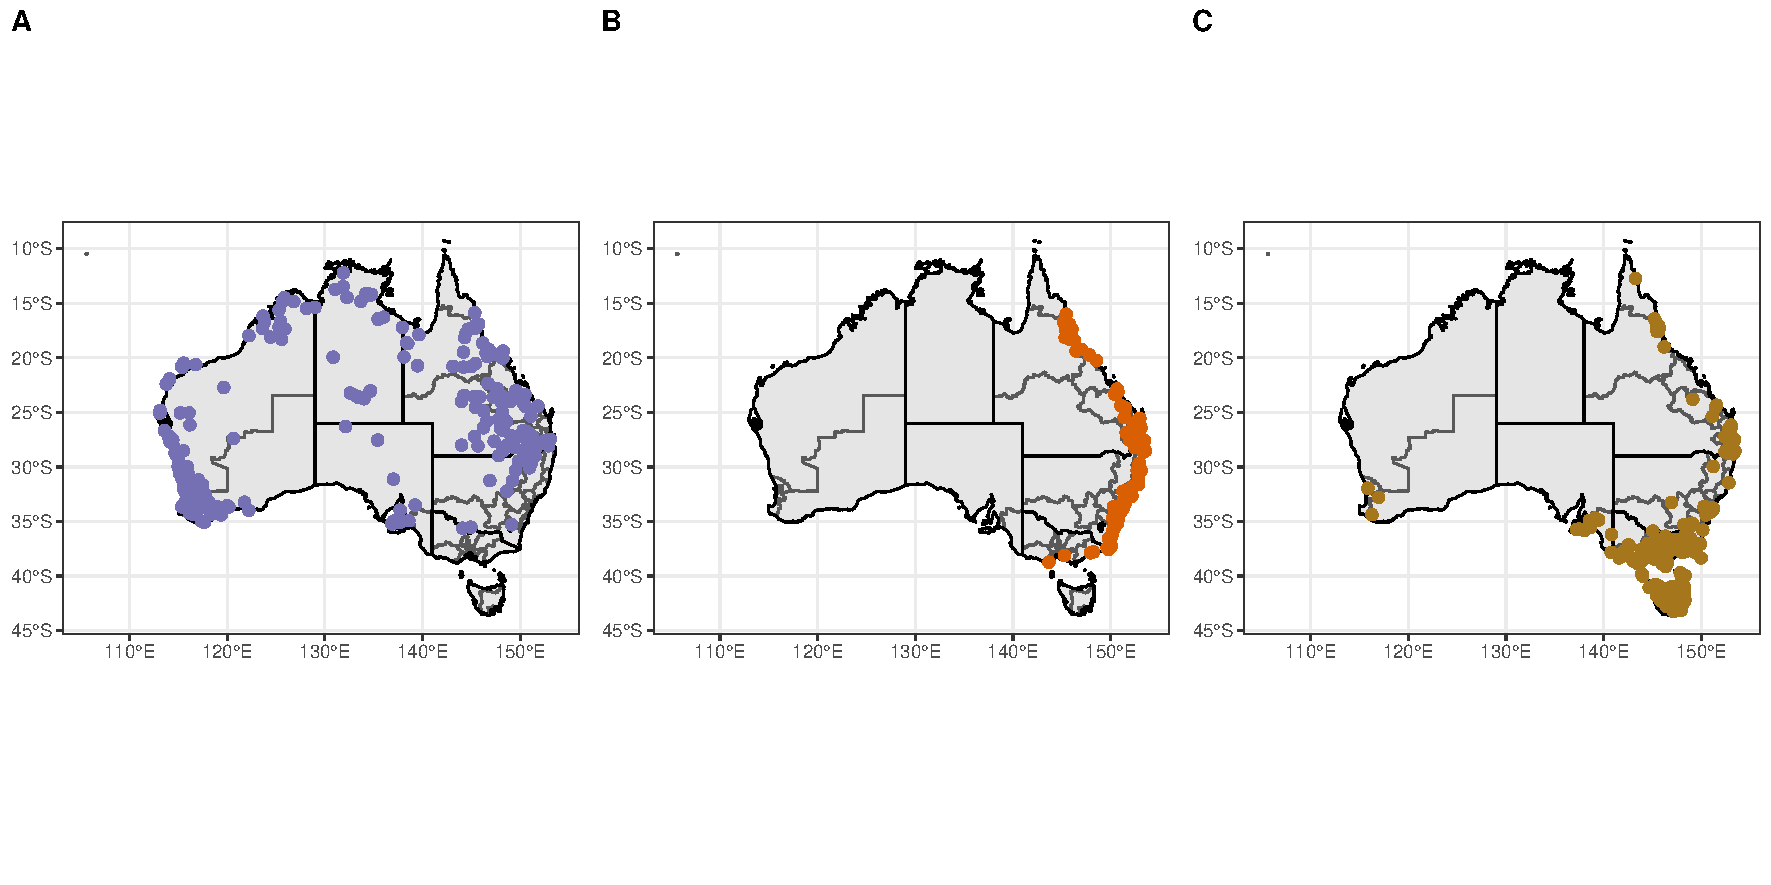
\includegraphics[width=0.95\linewidth]{front-and-back-matter/preface/tickmaps}

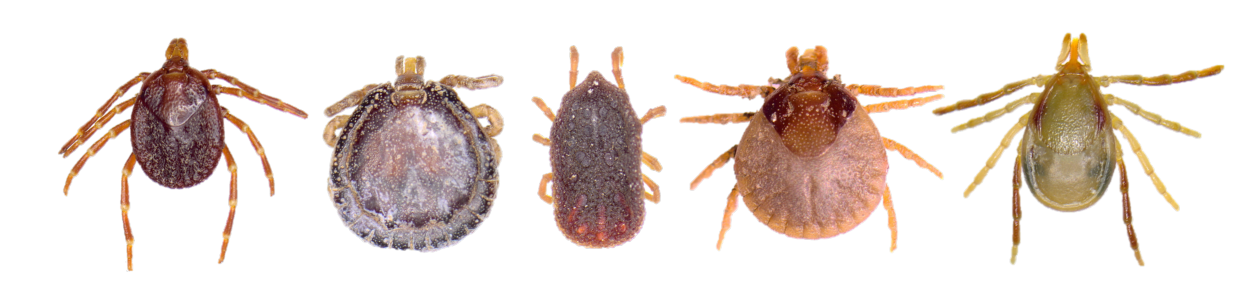
\includegraphics[width=0.95\linewidth]{front-and-back-matter/preface/austicks}

\newpage

\hypertarget{preface-1}{%
\section*{Preface}\label{preface-1}}
\addcontentsline{toc}{section}{Preface}

\textbf{Attribution Statement}

The following chapter has been drafted in accordance with the journal BMC Research Notes.

The following manuscript will be submitted: \textbf{Egan, S.}, Evans, M., Fontaine, J., Ryan, U., Irwin, P., and Oskam C. (\emph{To be submitted}). Australian ticks - Distribution, Hosts and Genetic identification of Ixodida.

The following authors contributed to this manuscript as outlined below\footnote{Contribution indicates the total involvement the author has had in this project. Placing an `X' in the remaining boxes indicates what aspect(s) of the project each author engaged in.}.

\begin{table}[!h]
\centering\begingroup\fontsize{7}{9}\selectfont

\begin{tabular}{lrllll}
\toprule
Authorship order & Contribution (\%) & Concept Development & Data Collection & Data Analyses & Drafting of manuscript\\
\midrule
\cellcolor{gray!6}{Siobhon L. Egan} & \cellcolor{gray!6}{80.0} & \cellcolor{gray!6}{X} & \cellcolor{gray!6}{X} & \cellcolor{gray!6}{X} & \cellcolor{gray!6}{X}\\
Megan Evans & 2.5 &  &  & X & \\
\cellcolor{gray!6}{Joseph Fontaine} & \cellcolor{gray!6}{2.5} & \cellcolor{gray!6}{} & \cellcolor{gray!6}{X} & \cellcolor{gray!6}{} & \cellcolor{gray!6}{}\\
Una M. Ryan & 5.0 & X &  &  & \\
\cellcolor{gray!6}{Peter J. Irwin} & \cellcolor{gray!6}{5.0} & \cellcolor{gray!6}{X} & \cellcolor{gray!6}{} & \cellcolor{gray!6}{} & \cellcolor{gray!6}{}\\
Charlotte L. Oskam & 5.0 & X &  &  & \\
\bottomrule
\end{tabular}
\endgroup{}
\end{table}

By signing this document, the Candidate and Principal Supervisor acknowledge that the information provided is accurate and has been agreed to by all other authors.

\vspace{3mm}

\raggedright

\_\_\_\_\_\_\_\_\_\_\_\_\_\_\_\_\_\_ ~ ~ ~ \_\_\_\_\_\_\_\_\_\_\_\_\_\_\_\_\_\_\\
\hspace*{0.333em}\hspace*{0.333em}Candidate ~ ~ ~ ~ ~ ~ ~ ~ ~ ~ ~ ~ ~ ~ ~ ~ Principal Supervisor

\newpage

\textbf{Chapter linking statement:}

This chapter is written as a ``data resource'' to synthesize information about Australian ticks.
Curation of records has been performed using data collected from a diverse range of sources.
Updated occurrence maps for three highly prevalent species; \emph{Amblyomma triguttatum}, \emph{Ixodes holocyclus} and \emph{Ixodes tasmani} are presented along with an overall map of all 74 tick species present in Australia. This chapter also presents new genetic information for Australian ticks.
Molecular ``barcodes'' are presented for target mitochondrial loci, providing valuable genetic references for species identification. In addition, a \hl{high-throughput sequencing} assay is also described using pan-Ixodida primers.
This provides a high-throughput method to identify ticks by sequencing a \textasciitilde370 bp product of the 12S rDNA gene on the Illumina MiSeq.
This chapter contains information gathered from a range of resources.
It is presented in the context of a data centric chapter, and will be submitted to journal BMC Research Notes in the format for a `Research Note'.

Discussion of the data presented here is provided however to avoid repetition from the previous chapter (literature review) and in accordance with journal requirements (2000 word limit for main text) the overarching aim here, is to provide a central forum for the synthesis of newly generated and curated data.

\vspace{5mm}

\textbf{Acknowledgment statement:}
Thank you to Dr.~Bruce Halliday (Australian National Insect Collection, CSIRO) for access to records and loan of specimens, Dr.~Mark Harvey (Western Australia Museum) and Dr.~Owen Seeman (Queensland Museum) for access to records and Prof.~Ian Beveridge (Melbourne University) for providing advice on tick records and collections.
We acknowledge the use of the Atlas of Living Australia, (\url{https://www.ala.org.au/}).
We acknowledge that use of records presented in this manuscript has been made possible by the work of previous researchers, we thank them for data collection and curation that has allowed us to conduct this work.

\vspace{5mm}

\textbf{Funding statement:}
This study was part-funded by the Australian Research Council (LP160100200), Bayer HealthCare (Germany) and Bayer Australia.
S.L.E. was supported by an Australian Government Research Training Program (RTP) Scholarship.
This project was also part supported by The Holsworth Wildlife Research Endowment \& The Ecological Society of Australia (awarded to S.L.E).

\vspace{5mm}

\textbf{Data availability:}

The datasets generated during the current study have been made available in the public repositories and the code used in analysis is available on GitHub.
Illumina MiSeq data generated from the metabarcoding of ticks targeting the 12S rRNA gene has been deposited in the European nucleotide archive under the project accession number PRJEB46056 (ERP130244), which includes the following sample accession numbers: ERS6635126--ERS6635348 (BioSample \# SAMEA8952359--SAMEA8952582).
Nucleotide data for a subset of zOTUs generated are available for the molecular identification of ticks and has been uploaded to GenBank under accession numbers MW665133--MW665150.
Nucleotide data for multilocus sequence typing (MLST) barcode sequence data produced by Sanger sequencing has been deposited in GenBank under the following accession numbers: OM791407--OM791437 (\emph{COI}), OM756760--OM756765 (\emph{18S rRNA}), OM830716--OM830764 (\emph{12S rDNA}), OM830384--OM830429 (\emph{16S rRNA}).
Code used for analysis and supporting data files used for bioinformatics and statistical analysis are available on GitHub repository \href{https://github.com/siobhon-egan/wildlife-ticks}{github.com/siobhon-egan/wildlife-ticks} and the \href{https://siobhonlegan.com/wildlife-ticks/}{project website}.

\vspace{5mm}

\textbf{Ethics:}
This study was conducted under the compliance of the Australian Code for the Responsibility Conduct of Research (2007) and Australian Code for the Care and Use of Animals for Scientific Purposes, 2013.
No specific animal research was conducted for the purposes of this work. Ticks from wildlife were collected as part of established research projects.

\textbf{Keywords:} Ixodida, \emph{Amblyomma triguttatum}, \emph{Ixodes holocyclus}, \emph{Ixodes tasmani}, molecular barcoding

\newpage

\hypertarget{abstract}{%
\section{Abstract}\label{abstract}}

To date 74 tick species have been recorded in Australia which include 60 Ixodidae (hard ticks) and 14 Argasidae (soft ticks).
Much of the fundamental knowledge of Australian ticks such as species records and occurrence maps are distributed throughout the scientific literature.
This scattered nature can it make it difficult for non-specialists to access basic information, thus, in the present study a synthesis of Australian tick records is provided.
A review of tick records and the incidences of humans as hosts, revealed a total of 28 species biting humans.
Updated occurrence maps revealed that three widespread tick species \emph{Amblyomma triguttatum}, \emph{Ixodes holocyclus} and \emph{Ixodes tasmani} also represent the most common species identified biting humans.
The present study also provides a review of records including curation of those provided in public databases; a \href{https://siobhonlegan.com/wildlife-ticks/}{companion website} also provides interactive maps of these records for readers to investigate.
In addition, new genetic data has been generated for mitochondrial loci from Australian ticks.
This information has been deposited in a public database (GenBank) and will assist in future efforts that seek to use molecular tools to confirm species identification.
The analysis of mitochondrial loci identified the 12S rDNA gene (\textasciitilde370 bp product) was particularly useful at delimitating species.
As a result, a \hl{high-throughput sequencing} assay was developed for high-throughput species identification.
The curation of records and genetic data generated here provide new insights in Australian ticks.
The findings reported here will be useful to shed new light for future studies on the ecology and systematics of ticks in Australia and be important in assessing public health significance of ticks as vectors for disease.

\hypertarget{introduction}{%
\section{Introduction}\label{introduction}}

Ticks \hl{(Acari: Ixodida)} parasitise a range of vertebrate hosts and serve as vectors for numerous pathogens that affect both humans and animals.
Occurrence records of tick species are a valuable tool that is of interest to medical and veterinary industries.

Tick species distribution records provide fundamental information that is required to assess the public health risk in relationship to diseases that ticks can cause.
Curation of these records is a pain-staking process and requires extensive searching not only in published journal articles but also in the `grey' literature and unpublished data sets such as those contained within university theses, government reports, etc \autocite{estrada-penaSpeciesOccurrenceTicks2019}.
Specimen collections housed by museums, universities, and research groups also provide a wealth of information that may not be easily accessible.
Online databases, particularly those where members of the public can submit records, can also provide useful information to build occurrence data \autocite{belbinAtlasLivingAustralia2021}.
However, careful consideration of the content of such records may be required where non-experts are providing identifications.

The aim of this study was to provide an update on records of Australian ticks.
The present study provides: (i) a list of tick species in Australia and identification of records for human biting ticks; (ii) updated distribution maps for three widespread tick species and an occurrence map with records of all 74 Australian tick species; (iii) a review of host records for the most widespread tick species in Australia, \emph{Amblyomma triguttatum}; (iv) new genetic data generated from ticks, useful as reference information for identifications; and finally (v) description and validation of a high-throughput assay for molecular identification of species

\hypertarget{main-text}{%
\section{Main text}\label{main-text}}

\hypertarget{methods}{%
\subsection{Methods}\label{methods}}

\hypertarget{tick-records}{%
\subsubsection{Tick records}\label{tick-records}}

Records were sourced from the Australian National Insect Collection (ANIC), the Western Australia Museum (WAM), Cryptick Laboratory tick archive (Murdoch University) and the literature (including a thorough review of grey literature, e.g., government reports).
The \href{https://www.ala.org.au/}{Atlas of Living Australia} was also investigated to identify records of tick species.
Due to the known issues with accurate identification of records in the Living Atlas Australia database \autocite{belbinAtlasLivingAustralia2021}, this data was further investigated.
Tick species with occurrence records outside of their known historic distribution area were verified for likelihood of accurate identification.

Host common names and scientific names are included and follow current taxonomic guidelines as described for mammals \autocite{jacksonTaxonomyAustralianMammals2015}, except where the taxonomic status has since been updated.

\textbf{Most prevalent species}\\
The three most common species identified from the analysis above were then selected to produce individual species maps.
This also included a more detailed curation of records from the grey literature.
As the most abundant and widespread species identified, further investigation of sporadic \emph{Am. triguttatum} was performed to confirm specimen identification.
Tick specimens that were not identified to species level in the ANIC Ixodida collection from New South Wales, Victoria and Tasmania were examined.
Historically \emph{Am. triguttatum} records from these regions have been scarce, and a confirmed identification from these areas could vastly expand the recognised distribution of \emph{Am. triguttatum}.
Due to the widespread nature of \emph{Am. triguttatum} a list of host records was also synthesied for this species.

\hypertarget{tick-identification}{%
\subsubsection{Tick identification}\label{tick-identification}}

Samples were visualised using an Olympus SZ61 stereomicroscope (Olympus, Centre Valley, PA, United States) with an external Schott KL 1500 LED (Schott AG Mainz, Germany) light source.
Photographs of tick specimens were taken using an Olympus SC30 digital camera (Olympus, Centre Valley, PA, United States) and analysis getIT software (Olympus, Centre Valley, PA, United States).
Instar, sex, and species was identified using a combination of available morphological keys and species descriptions \autocite{robertsAustralianTicks1970,jacksonMorphologicalComparisonAdult2002,laanObservationsBiologyDistribution2011,barkerTicksAustraliaSpecies2014,kwakPhylogeneticAnalysisAustralian2017}.
Where possible \emph{Am. triguttatum} specimens were assigned to subspecies according to that described in \textcite{robertsStatusMorphologicallyDivergent1962}.

\hypertarget{genetic-analysis-of-ticks}{%
\subsubsection{Genetic analysis of ticks}\label{genetic-analysis-of-ticks}}

\textbf{Sample collection}\\
Specimens in the Cryptick Laboratory tick archive were used for molecular assays and generation of new sequence data.
These ticks were collected since 2016 from various sources such as wildlife rehabilitation centres, veterinary clinics and research projects including collection of ticks from the environment or from wildlife.
In the case of ticks collected from wildlife, samples were collected as part of the research project described in Chapters \ref{wildlife-bacteria} and \ref{wildlife-haemoprotozoa}.

\textbf{DNA extraction and sequencing}\\
The complete details of the methods is described in the \ref{ch2supp}.
In brief, DNA was extracted from ticks and two molecular approaches were used: (i) multi-locus sequence typing (MSLT) assays with Sanger sequencing and (ii) development of a high-throughput assay to identify ticks.

For the MLST assays, primers were used to amplify ticks at the following mitochondrial loci: \emph{cytochrome c oxidase subunit I} (\emph{COX1}) \autocite{songPhylogeneticPhylogeographicRelationships2011}, \emph{12S rDNA} \autocite{beatiAnalysisSystematicRelationships2001}, \emph{16S rDNA} \autocite{lvDevelopmentDNABarcoding2014} (see Table \ref{tab:T2primers}).
Purified PCR products were then subjected to Sanger sequencing in the forward and reverse direction.

Following the results from the MLST approach, the \textasciitilde370 bp product of the 12S rDNA gene was determined as providing optimal results for species delimitation.
In addition, the short fragment size made it suitable to transfer the assay onto the Illumina MiSeq platform.
In brief, extracted tick DNA was used to build libraries following the 16S Metagenomic Sequencing Library Preparation (Illumina Part \# 15044223 Rev.~B).
The amplicon PCR was carried out using the 12S rDNA gene pan-Ixodida primers, T1B and T2A \autocite{beatiAnalysisSystematicRelationships2001} (\textasciitilde370 bp product) with Illumina MiSeq adapters (Table \ref{tab:T2primers}).
Libraries were then constructed and sequenced on the Illumina MiSeq using v2 chemistry (2 x 250 paired end).

\hypertarget{data-analysis-and-bioinformatics}{%
\subsubsection{Data analysis and bioinformatics}\label{data-analysis-and-bioinformatics}}

Distribution maps were produced in RStudio \autocite{rstudioteamRStudioIntegratedDevelopment2015}.
Maps of Australia were drawn using ozmaps \autocite{SumnerOzmaps2021}, sf \autocite{PebesmaRsf2018} and sp \autocite{BivandRsp2013} R packages.

Sequences obtained from MLST assays were imported into Geneious 10.2.6 (\url{https://www.geneious.com}) for quality inspection.
Illumina MiSeq data was analysed using a bioinformatic pipeline with the program USEARCH v11 \autocite{edgarSearchClusteringOrders2010} with zero radius operational taxonomic units generated (zOTUs).
All sequences were subject to BLAST analysis (BLASTN 2.11.0+ \autocite{zhangGreedyAlgorithmAligning2000,morgulisDatabaseIndexingProduction2008}) against the NCBI nucleotide collection (nt) database to confirm identification.

Full details of analysis methods are available in supplementary material \ref{ch2supp} and at the repository \url{https://github.com/siobhon-egan/wildlife-ticks}.

\hypertarget{results-and-discussion}{%
\subsection{Results and Discussion}\label{results-and-discussion}}

\hypertarget{australian-ticks}{%
\subsubsection{Australian ticks}\label{australian-ticks}}

A list of all 74 tick species recorded in Australia is presented in Table \ref{tab:T2humanrecords} and includes 60 hard ticks and 14 soft ticks.
Five tick species are identified as introduced and are associated with domesticated livestock and companion animals; these include two soft ticks \emph{Argas persicus} (associated with poultry) and \emph{Otobius megnini} (imported with horses); and three hard ticks, \emph{Haemaphysalis longicornis} (associated with cattle), \emph{Rhipicephalus linnaei} (syn \emph{Rhipicephalus sanguineus} tropical lineage) (associated with dogs) and \emph{Rhipicephalus australis} (syn \emph{Boophilus microplus}) (associated with cattle).

\textbf{Human records}\\
A review of human incidents of tick bite in Australia identified 28 species reported.
In many cases records of species biting humans are confined to sporadic single identifications (Table \ref{tab:T2humanrecords}).
It is noted that reporting of a ``human'' record with ticks reveals little regarding the potential significance for zoonotic tick-borne diseases.
The identification of ticks from human hosts does not necessarily distinguish if the tick was attached and actively feeding, or if the tick was simply found crawling on the individual.
While this omission might seem trivial it is a key piece of information in establishing an accurate list of host records, particularly where records of the tick-host association are sparse.
In addition, it is important to note in regard to tick-borne diseases, the tick vector remains just one of three components in the cycle of tick-borne pathogens; the dynamics of microbe and reservoir host(s) are also requirements for a zoonotic pathogen to become endemic.
Identification of incidents, referred to as ``tick encounters'', may prove a more useful tool to quantify the risk of tick bites to people.
While this field of research has been conducted in the northern hemisphere \autocite{hookHumanTickEncounters2021}, similar studies have not been conducted in Australia.

The list of human-tick records in Australia includes a diverse range of species however, the overwhelming evidence concludes that \emph{Ix. holocyclus} and \emph{Am. triguttatum} contribute to the vast majority (\textgreater90\%) of tick bites \autocite{goftonBacterialProfilingReveals2015,geary30YearsSamples2020}.
An interesting observation in the literature was the identification of the platypus tick \emph{Ixodes ornithorynchi} from a human in northern Victoria \autocite{geary30YearsSamples2020}. The specimen was submitted from a wildlife carer who had direct contact with platypus. In addition to the 28 species reporting biting human two tick species, \emph{Argas lagenoplastis} and \emph{Ornithodorus macmillani} were noted by \textcite{geary30YearsSamples2020} from birds' nests but were not directly associated with biting humans.

This review has provided a synthesis of tick-host records in Australia.
It is evident that some publications have reported a ``new'' host record, however review of extant museum collections or historic data has shown it had been previously recorded.
For example, an incidence of \emph{Ix. australiensis} biting a human was reported as a first record by \textcite{kwakFirstRecordsHuman2018}, occurring in October 2017.
However, \textcite{rabyNewFociSpotted2016}, reported the tick biting a person in May 2006.
In addition, we note that \emph{Ix. australiensis} wwas reported in close association with humans by \textcite{robertsAustralianTicks1970}, however it was noted the tick was ``crawling''. An exhaustive review of all host records is not practical where the data is widely distributed in the literature; this serves to demonstrate the value of curated data, especially where it has the potential to be of public health significance.

\begin{landscape}\begingroup\fontsize{8}{10}\selectfont

\begin{longtable}[t]{>{\raggedright\arraybackslash}p{4cm}>{\raggedright\arraybackslash}p{3cm}>{\raggedright\arraybackslash}p{1cm}>{\raggedright\arraybackslash}p{4cm}>{\raggedright\arraybackslash}p{6cm}}
\caption[Tick species of Australia.]{\label{tab:T2humanrecords}List of tick species recorded from Australia. Human records indicated by colour.}\\
\toprule
Species & Authority & H (a) & Hosts & Notes\\
\midrule
\endfirsthead
\caption[]{\label{tab:T2humanrecords}List of tick species recorded from Australia. Human records indicated by colour. \textit{(continued)}}\\
\toprule
Species & Authority & H (a) & Hosts & Notes\\
\midrule
\endhead

\endfoot
\bottomrule
\multicolumn{5}{l}{\rule{0pt}{1em}\textsuperscript{a} Reference of human biting ticks sourced from published and grey literature including museum records.}\\
\endlastfoot
\textit{Amblyomma albolimatum} (stump-tailed lizard tick ) & Neumann 1907 & \multicolumn{1}{c}{\cellcolor[HTML]{8DD3C7}{\textcolor{white}{Y}}} & Reptiles (lizards and snakes) & Similar to \textit{Amblyomma limbatum}\\
\textit{Amblyomma australiense} & Neumann 1905 & \multicolumn{1}{c}{\cellcolor[HTML]{BEBADA}{\textcolor{white}{N}}} & Echidna (possibly reptiles) & Inornate species. Very few records, description from long-beaked echidna, \textit{Zaglossus bruijnii} (now regionally extinct) in Western Australia (historical). Most similar to \textit{Amblyomma echidnae}.\\
\textit{Amblyomma breviscutatum} & Neuman 1899 & \multicolumn{1}{c}{\cellcolor[HTML]{BEBADA}{\textcolor{white}{N}}} & Pigs, rodents & Syn. \textit{Amblyomma cyprium}. Few records of this in Australia.\\
\textit{Amblyomma calabyi} (Calaby's goanna tick) & Roberts 1963 & \multicolumn{1}{c}{\cellcolor[HTML]{BEBADA}{\textcolor{white}{N}}} & Reptiles (large monitor lizards) & \\
\textit{Amblyomma echidnae} & Roberts 1953 & \multicolumn{1}{c}{\cellcolor[HTML]{BEBADA}{\textcolor{white}{N}}} & Echidna & Morphologically similar to \textit{Amblyomma australiense}.\\
\textit{ Amblyomma fimbriatum} (tropical reptile tick) & Koch 1844 & \multicolumn{1}{c}{\cellcolor[HTML]{BEBADA}{\textcolor{white}{N}}} & Reptiles (lizards and snakes) & Previously \textit{Aponomma} (eye-less \textit{Amblyomma}). Syn. \textit{Aponomma ecinctum}.\\
\textit{Amblyomma glauerti} & Keirans, King and Sharrad 1994 & \multicolumn{1}{c}{\cellcolor[HTML]{BEBADA}{\textcolor{white}{N}}} & Reptiles (lizards) & \\
\textit{Amblyomma limbatum} (reptile tick) & Neumann 1899 & \multicolumn{1}{c}{\cellcolor[HTML]{8DD3C7}{\textcolor{white}{Y}}} & Reptiles (lizards and snakes) & Similar to \textit{Amblyomma albolimbatum}; In addition historical identifications maybe confused with \textit{Amblyomma moreliae}.\\
\textit{Amblyomma loculosum} (seabird tick) & Neumann 1907 & \multicolumn{1}{c}{\cellcolor[HTML]{8DD3C7}{\textcolor{white}{Y}}} & Seabirds & Syn. \textit{Amblyomma sternae} Roberts 1953.\\
\textit{Amblyomma macropi} & Roberts 1953 & \multicolumn{1}{c}{\cellcolor[HTML]{BEBADA}{\textcolor{white}{N}}} & Kangaroos & Very few records, only from "kangaros" in north east QLD.\\
\textit{Amblyomma moreliae} (snake tick) & Koch 1867 & \multicolumn{1}{c}{\cellcolor[HTML]{8DD3C7}{\textcolor{white}{Y}}} & Reptiles (snakes) & Previously thought to be subspecies of \textit{Amblyomma limbatum}. Syn \textit{Ixodes moreliae}.\\
\textit{Amblyomma moyi} & Roberts 1953 & \multicolumn{1}{c}{\cellcolor[HTML]{BEBADA}{\textcolor{white}{N}}} & Echidna & \\
\textit{Amblyomma papuanum} & Hirt 1914 & \multicolumn{1}{c}{\cellcolor[HTML]{BEBADA}{\textcolor{white}{N}}} & Echidna & \\
\textit{Amblyomma postoculatum} & Neumann 1899 & \multicolumn{1}{c}{\cellcolor[HTML]{8DD3C7}{\textcolor{white}{Y}}} & Wallaby and kangaroos & \\
\textit{Amblyomma triguttatum} (ornate kangaroo tick) & Koch 1844 & \multicolumn{1}{c}{\cellcolor[HTML]{8DD3C7}{\textcolor{white}{Y}}} & Various mammals (kangaroos) & Four subspecies as described by Roberts 1962.\\
\textit{Amblyomma trimaculatum} & Lucas 1878 & \multicolumn{1}{c}{\cellcolor[HTML]{BEBADA}{\textcolor{white}{N}}} & Reptiles (lizards and snakes) & Previously \textit{Aponomma}, (eye-less \textit{Amblyomma}). Syn \textit{Ixodes trimaculatum}.\\
\textit{Amblyomma vikirri} & Keirans, Bull and Duffield 1996 & \multicolumn{1}{c}{\cellcolor[HTML]{BEBADA}{\textcolor{white}{N}}} & Reptiles (lizards) & Can be confused with \textit{Amblyomma glauerti} and sometimes \textit{Amblyomma limbatum}. \textit{Amblyomma vikirri} is ornamented with a light background coloration, little ornamentation in the scapular areas and ornamentation on all festoons.\\
\textit{Bothriocroton auruginans} (wombat tick) & Schulze 1936 & \multicolumn{1}{c}{\cellcolor[HTML]{8DD3C7}{\textcolor{white}{Y}}} & Wombats & \\
\textit{Bothriocroton concolor} (short-beaked echidna tick) & Neumann 1899 & \multicolumn{1}{c}{\cellcolor[HTML]{BEBADA}{\textcolor{white}{N}}} & Echidna & Often confusion with \textit{Bothriocroton tachyglossi} in earlier descriptions. Changes in taxonomy mean many syn. names over time e.g. \textit{Aponomma concolor}, \textit{Aponomma hydrosauri}, \textit{Aponomma tropicum}.\\
\textit{Bothriocroton glebopalma} & Keirans, King and Sharrad 1994 & \multicolumn{1}{c}{\cellcolor[HTML]{BEBADA}{\textcolor{white}{N}}} & Reptiles (lizards) & \\
\textit{Bothriocroton hydrosauri} (southern reptile tick) & Denny 1843 & \multicolumn{1}{c}{\cellcolor[HTML]{8DD3C7}{\textcolor{white}{Y}}} & Reptiles (lizards and snakes) & Female holotype maybe \textit{Aponomma tachyglossi} or \textit{Aponomma concolor}. Previous indentifications remain elusive as syn. with many species in earlier descriptions (e.g. \textit{Bothriocroton tachyglossi}, \textit{Bothriocroton concolor}, and \textit{Aponomma trachysauri} to name a few). Syn \textit{Ixodes hydrosauri}, \textit{Aponomma trachysauri}, \textit{Aponomma tachyglossi}.\\
\textit{Bothriocroton tachyglossi} (central Queensland short-beaked echidna tick) & Roberts 1953 (re-instated by Andrews et al. 2006) & \multicolumn{1}{c}{\cellcolor[HTML]{BEBADA}{\textcolor{white}{N}}} & Echidna & Although described by Roberts in 1960, later considered a subsp. of \textit{Bothriocroton hydrosauri} and therefore not recognised in Roberts 1970 keys. Andrews et al. 2006 provided more detailed description and raised it to species status.\\
\textit{Bothriocroton undatum} (goana tick) & Fabricius 1775 & \multicolumn{1}{c}{\cellcolor[HTML]{8DD3C7}{\textcolor{white}{Y}}} & Reptiles (lizards ), echidna & Syn. \textit{Acras undatus}, \textit{Ixodes decorosus}, \textit{Aponomma decorosum}.\\
\textit{Haemaphysalis bancrofti} (wallaby tick) & Nuttall and Warburton 1915 & \multicolumn{1}{c}{\cellcolor[HTML]{8DD3C7}{\textcolor{white}{Y}}} & Wallabies and kangaroos & Historical records show it may have been confused with \textit{Haemaphysalis doenitzi}. Syn with \textit{Haempahysalis meraukensis}, \textit{Haemaphysalis krijgsmani}.\\
\textit{Haemaphysalis bremneri} (Bremner’s possum tick) & Roberts 1963 & \multicolumn{1}{c}{\cellcolor[HTML]{BEBADA}{\textcolor{white}{N}}} & Possum & Can be confused with \textit{Haemaphysalis humerosa} or \textit{Haemaphysalis ratti}.\\
\textit{Haemaphysalis doenitzi} (Ooenitz Oriental – Australian bird haemaphysalid) & Warburton and Nuttall 1909 & \multicolumn{1}{c}{\cellcolor[HTML]{8DD3C7}{\textcolor{white}{Y}}} & Birds & Presence in Australia is recognised but not well documented.\\
\textit{Haemaphysalis humerosa} (bandicoot tick) & Warburton and Nuttall 1909 & \multicolumn{1}{c}{\cellcolor[HTML]{8DD3C7}{\textcolor{white}{Y}}} & Various mammals (bandicoots, wallabies, rodents) & Can be confused with \textit{Haemaphysalis bremneri} or \textit{Haemaphysalis ratti}.\\
\textit{Haemaphysalis lagostrophi} & Roberts 1963 & \multicolumn{1}{c}{\cellcolor[HTML]{BEBADA}{\textcolor{white}{N}}} & Wallabies and bandicoot & \\
\textit{Haemaphysalis longicornis} (bush tick) & Neumann 1901 & \multicolumn{1}{c}{\cellcolor[HTML]{8DD3C7}{\textcolor{white}{Y}}} & Various mammals (kangaroos) & Introduced.Syn. \textit{Haemaphysalis bispinosa} Nuttall and Warburton 1915 (record presence in Australia),  \textit{Haemaphysalis neumanni}.\\
\textit{Haemaphysalis novaeguinae} & Hirt 1914 & \multicolumn{1}{c}{\cellcolor[HTML]{8DD3C7}{\textcolor{white}{Y}}} & Mammal & Syn with \textit{Haemaphysalis  spinigera var. novaeguineae}.\\
\textit{Haemaphysalis petrogalis} (rock-wallaby tick) & Roberts 1970 & \multicolumn{1}{c}{\cellcolor[HTML]{BEBADA}{\textcolor{white}{N}}} & Mammal (wallabies) & \\
\textit{Haemaphysalis ratti} (rat tick) & Kohls 1948 & \multicolumn{1}{c}{\cellcolor[HTML]{BEBADA}{\textcolor{white}{N}}} & Mammal (rats and small marsupials) & Can be confused with \textit{Haemaphysalis humerosa} or \textit{Haemaphysalis bremneri}.\\
\textit{Ixodes antechini} (Antechinus tick) & Roberts 1960 & \multicolumn{1}{c}{\cellcolor[HTML]{BEBADA}{\textcolor{white}{N}}} & Small mammals (antechinus) & \\
\textit{Ixodes auritulus} (New Zealand seabird tick) & Neumann 1904 & \multicolumn{1}{c}{\cellcolor[HTML]{BEBADA}{\textcolor{white}{N}}} & Seabirds & Can be confused with \textit{Ixodes fecialis}.\\
\textit{Ixodes australiensis} & Roberts 1960 & \multicolumn{1}{c}{\cellcolor[HTML]{8DD3C7}{\textcolor{white}{Y}}} & Mammals (kangaroos, bandicoots, possums) & \\
\textit{Ixodes barkeri} & Barker 2019 & \multicolumn{1}{c}{\cellcolor[HTML]{BEBADA}{\textcolor{white}{N}}} & Echidna & Distinct horn-like projection on palpal article 1. Some similar to \textit{Ixodes zaglossi} Kohls, 1960 from the long-beaked echidna of Papua New Guinea.\\
\textit{Ixodes confusus} & Roberts 1960 & \multicolumn{1}{c}{\cellcolor[HTML]{8DD3C7}{\textcolor{white}{Y}}} & Mammals (possums, bandicoots) & Records of this tick in Australia are sparse (previous confused with \textit{Ixodes cordifer}), Roberts 1970 reports just a single specimen, a female from Innisfail north Queensland.\\
\textit{Ixodes cordifer} & Neumann 1908 & \multicolumn{1}{c}{\cellcolor[HTML]{BEBADA}{\textcolor{white}{N}}} & Mammals (possums, rodents) & \\
\textit{Ixodes cornuatus} (southern paralysis tck) & Roberts 1960 & \multicolumn{1}{c}{\cellcolor[HTML]{8DD3C7}{\textcolor{white}{Y}}} & Various mammals (possums, wallabies, rodents) & Earlier records difficult to conclude due to similarity with \textit{Ixodes holocyclus}.\\
\textit{Ixodes eudyptidis} & Maskell 1885 & \multicolumn{1}{c}{\cellcolor[HTML]{BEBADA}{\textcolor{white}{N}}} & Seabirds & \\
\textit{Ixodes fecialis} & Warburton and Nuttall 1904 & \multicolumn{1}{c}{\cellcolor[HTML]{8DD3C7}{\textcolor{white}{Y}}} & Various mammals (kangaroos, bandicoots, possums, wallabies, rodents) & Similar to \textit{Ixodes fecialis}.\\
\textit{Ixodes heathi} (mountain pygmy possum tick) & Kwak, Madden and Wicker 2018 & \multicolumn{1}{c}{\cellcolor[HTML]{BEBADA}{\textcolor{white}{N}}} & Mountain pygmy possum & \\
\textit{Ixodes hirsti} (Hirst's marsupial tick) & Hassall 1931 & \multicolumn{1}{c}{\cellcolor[HTML]{8DD3C7}{\textcolor{white}{Y}}} & Various mammals (possums, wallabies, rodents) and birds & See Laan et al. 2011 for description of immature instars, and further details on adults.\\
\textit{Ixodes holocyclus} (paralysis tick) & Neumann 1899 & \multicolumn{1}{c}{\cellcolor[HTML]{8DD3C7}{\textcolor{white}{Y}}} & Various mammals (kangaroos, bandicoots, possums, wallabies, rodents) & \\
\textit{Ixodes hydromyidis} (water rat tick) & Swan 1931 & \multicolumn{1}{c}{\cellcolor[HTML]{BEBADA}{\textcolor{white}{N}}} & Rodents & \\
\textit{Ixodes kerguelenensis} & Andre and Colas-Belcour 1942 & \multicolumn{1}{c}{\cellcolor[HTML]{BEBADA}{\textcolor{white}{N}}} & Seabirds & Many syns: \textit{Ixodes canisuga kerguelenensis, Ixodes canisuga var. kerguelenensis, Ixodes percavatus, Ixodes pterodromae, Ixodes zumpti, Ixodes (Multidentatus) kerguelenensis, Scaphixodes (Multidentatus) kerguelenensis}.\\
\textit{Ixodes kohlsi} & Arthur 1955 & \multicolumn{1}{c}{\cellcolor[HTML]{8DD3C7}{\textcolor{white}{Y}}} & Seabirds & \\
\textit{Ixodes kopsteini} (Kopstein's bat tick) & Oudemans 1926 & \multicolumn{1}{c}{\cellcolor[HTML]{BEBADA}{\textcolor{white}{N}}} & Bats & Very few records of this ticks in Australia. Roberts 1970 refers to a single Australian records based on personal communication. Record from Tadarida colonicus, Nicholson River Northern Territory.\\
\textit{Ixodes laridis} & Heath and Palma 2017 & \multicolumn{1}{c}{\cellcolor[HTML]{BEBADA}{\textcolor{white}{N}}} & Seabirds & Syn. \textit{Ixodes eudyptidis}\\
\textit{Ixodes myrmecobii} & Roberts 1962 & \multicolumn{1}{c}{\cellcolor[HTML]{8DD3C7}{\textcolor{white}{Y}}} & Numbat & Syn. \textit{Ixodes holocyclus} pre-1960. See Kwak et al. 2018 for new description of nymph and male and redescription of female.\\
\textit{Ixodes ornithorhynchi} (platypus tick) & Lucas 1846 & \multicolumn{1}{c}{\cellcolor[HTML]{8DD3C7}{\textcolor{white}{Y}}} & Platypus & \\
\textit{Ixodes simplex} (bat tick) & Neumann 1906 & \multicolumn{1}{c}{\cellcolor[HTML]{BEBADA}{\textcolor{white}{N}}} & Bats & \\
\textit{Ixodes tasmani} (common marsupial tick) & Neumann 1899 & \multicolumn{1}{c}{\cellcolor[HTML]{8DD3C7}{\textcolor{white}{Y}}} & Various mammals (kangaroos, bandicoots, possums, wallabies, rodents) & \\
\textit{Ixodes trichosuri} (possum tick) & Roberts 1960 & \multicolumn{1}{c}{\cellcolor[HTML]{BEBADA}{\textcolor{white}{N}}} & Mammals (possums, bandicoots) & See McCann et al. 2019. Reported high genetic diversity (2 distinct genotype, may have species status).\\
\textit{Ixodes uriae} & White 1852 & \multicolumn{1}{c}{\cellcolor[HTML]{BEBADA}{\textcolor{white}{N}}} & Seabirds & \\
\textit{Ixodes vestitus} (numbat tick) & Warburton and Nuttall 1909 & \multicolumn{1}{c}{\cellcolor[HTML]{BEBADA}{\textcolor{white}{N}}} & Numbat & \\
\textit{Ixodes victoriensis} & Nuttall 1916 & \multicolumn{1}{c}{\cellcolor[HTML]{BEBADA}{\textcolor{white}{N}}} & Wombats and macropods & See Weaver 2016 for detailed redescription of this species.\\
\textit{Ixodes woylei} (woylie tick) & Ash et al. 2017 & \multicolumn{1}{c}{\cellcolor[HTML]{BEBADA}{\textcolor{white}{N}}} & Woylie & Most similar to \textit{Ixodes victoriensis}, however these two species can be readily differentiated by dentition and the shape of the scutum, spurs on the coxae, and palpal article 1.\\
\textit{Rhipicephalus australis} (Australian cattle tick) & Fuller 1899 & \multicolumn{1}{c}{\cellcolor[HTML]{8DD3C7}{\textcolor{white}{Y}}} & Cattle & Introduced. Syn. \textit{Boophilus microplus, Boophilus australis}.\\
\textit{Rhipicephalus linnaei} (brown dog tick) & Latreille 1806 & \multicolumn{1}{c}{\cellcolor[HTML]{8DD3C7}{\textcolor{white}{Y}}} & Dogs & Introduced. Recent taxonomic change in 2021, previously \textit{Rhipicephalus sanguineus} tropical lineage. Since the recently described neotype of the species (See Nava et al 2018), a new name has been proposed based on molecular divergence (see Chandra et al. 2019 and Slapeta et al. 2021).\\
\textit{Argas falco} & Kaiser and Hoogstraal 1974 & \multicolumn{1}{c}{\cellcolor[HTML]{BEBADA}{\textcolor{white}{N}}} & Birds (kestrel) & \\
\textit{Argas lagenoplastis} (Australian fairy martin argasid) & Froggatt 1906 & \multicolumn{1}{c}{\cellcolor[HTML]{BEBADA}{\textcolor{white}{N}}} & Birds (fairy martin) & \\
\textit{Argas lowryae} (Lowryae's bird argasid) & Kaiser and Hoogstraal 1975 & \multicolumn{1}{c}{\cellcolor[HTML]{BEBADA}{\textcolor{white}{N}}} & Birds (kestrel) & \\
\textit{Argas nullarborensis} & Hoogstraal and Kaiser 1973 & \multicolumn{1}{c}{\cellcolor[HTML]{BEBADA}{\textcolor{white}{N}}} & Birds (crow) & \\
\textit{Argas persicus} (fowl tick) & Oken 1818 & \multicolumn{1}{c}{\cellcolor[HTML]{8DD3C7}{\textcolor{white}{Y}}} & Domestic poultry & Introduced.\\
\textit{Argas robertsi} (Robert's bird tick) & Hoogstraal, Kaiser and Kohls 1968 & \multicolumn{1}{c}{\cellcolor[HTML]{BEBADA}{\textcolor{white}{N}}} & Birds (egrets, domestic poultry) & \\
\textit{Carios australiensis} & Kohls and Hoogstraal 1962 & \multicolumn{1}{c}{\cellcolor[HTML]{BEBADA}{\textcolor{white}{N}}} & Bats (presumed) & Recent change of name (see Mans et al. 2019) previously \textit{Argas australiensis}.\\
\textit{Carios capensis} (seabird soft tick) & Neumann 1901 & \multicolumn{1}{c}{\cellcolor[HTML]{8DD3C7}{\textcolor{white}{Y}}} & Seabirds & Recent change of name (see Mans et al. 2019) previously \textit{Ornithodoros capensis}.\\
\textit{Carios daviesi} (Davies' bat argasid) & Kaiser and Hoogstraal 1973 & \multicolumn{1}{c}{\cellcolor[HTML]{BEBADA}{\textcolor{white}{N}}} & Bats & Recent change of name (see Mans et al. 2019) previously \textit{Argas daviesi}.\\
\textit{Carios dewae} (Dewae's bat argasid) & Kaiser and Hoogstraal 1974 & \multicolumn{1}{c}{\cellcolor[HTML]{BEBADA}{\textcolor{white}{N}}} & Bats & Recent change of name (see Mans et al. 2019) previously \textit{Argas dewae}.\\
\textit{Carios macrodermae} (ghost bat argasid) & Hoogstraal, Moorhouse, Wolf and Wassef 1977 & \multicolumn{1}{c}{\cellcolor[HTML]{BEBADA}{\textcolor{white}{N}}} & Bats & Recent change of name (see Mans et al. 2019) previously \textit{Argas macrodermae}.\\
\textit{Ornithodoros gurneyi} (kangaroo soft tick) & Warburton 1926 & \multicolumn{1}{c}{\cellcolor[HTML]{8DD3C7}{\textcolor{white}{Y}}} & associated with kangaroos & Despite its common name host records are very sparse, and no records of tick attached to host.\\
\textit{Ornithodoros macmillani} (possum soft tick) & Hoogstraal and Kohls 1966 & \multicolumn{1}{c}{\cellcolor[HTML]{BEBADA}{\textcolor{white}{N}}} & Various (possums, birds) & \\
\textit{Otobius megnini} (spinose ear tick) & Duges 1883 & \multicolumn{1}{c}{\cellcolor[HTML]{BEBADA}{\textcolor{white}{N}}} & Domestic horse & Introduced.\\*
\end{longtable}
\endgroup{}
\end{landscape}

\newpage

\hypertarget{distribution-maps}{%
\subsubsection{Distribution maps}\label{distribution-maps}}

An updated map of curated records for all 74 species of tick present in Australia is presented in Figure \ref{fig:F2mapall}.
Records without a species identification or those with missing location data were excluded.
A final dataset of 6,282 observation records was used to build the occurrence map (Figure \ref{fig:F2mapall}).

It was noted that two species were not present in any museum record searches.
\emph{Argas lowryae} was described by \textcite{kaiserObservationsSubgenusArgas1975}, and to the best of the authors' knowledge it has not been recorded since these initial observations.
Another soft tick, the invasive spinose ear tick \emph{Otobius mengini}, was also not identified from any museum records.
Instead, a single observation of the species in Perth, Western Australia, reported by the state government \autocite{mayberrySpinoseEarTick2003} was used in the occurrence map.
To complete the occurrence map, data for missing tick species was sourced from the literature.
Where possible, records for species that were outside of their historical distribution were individually inspected.

\textbf{Atlas of Living Australia data}

In comparison to the curated data (Figure \ref{fig:F2mapall}), a map of records based solely on data from Atlas of Living Australia was used to build an occurrence map.
This analysis only identified 57 species (50 hard ticks and seven soft ticks).
Once records with missing data (i.e., no species level identification) were removed, a total of 2,293 records were identified and used to the build map presented in Figure \ref{fig:FA21}.

\textbf{Most prevalent species}

The species with the highest number of observations were \emph{Am. triguttatum} (n = 1,286), \emph{Ix. tasmani} (n = 1,159), \emph{Ix. holocyclus} (n = 982), \emph{Ix. cornuatus} (n = 219), and \emph{Bt. auruginans} (n = 159).
The three most common species were then selected for further analysis, including a more detailed curation of records from the grey literature and individual species maps were produced.

Currently \emph{Am. triguttatum} is divided into four subspecies.
This has remained unchanged since it was established by \textcite{robertsStatusMorphologicallyDivergent1962}.
A total of 766 records were identified with subspecies status, of these 738 records had location information.
A distribution map of these four subspecies is presented in Figure \ref{fig:F2atrigmapsubp}.
After investigation of ``\emph{Am. triguttatum}'' specimens recorded in Tasmania and Victoria,
it was determined these were either incorrectly identified or incorrectly entered into databases.
In the case of records from Tasmania, these specimens were identified as \emph{Bt. hydrosauri}, while records from Victoria were assigned instead to either other \emph{Amblyomma} species or as members of the genus \emph{Bothriocroton}.
An example of incorrect records for this species is evident in the map produced using records collected from Atlas of Living Australia (Figure \ref{fig:FA21}).
\emph{Amblyomma triguttatum} is a widespread tick present throughout Australia from the south-west coast of Western Australia up to the northeast of Queensland.
At present the species is considered absent from Tasmania and Victoria, however an invasive population has established on the Yorke Peninsula in South Australia \autocite{mcdiarmidRangeExpansionTick2000}.

It is interesting that the distribution map (Figure \ref{fig:F2atrigmapsubp}) of \emph{Am. triguttatum} has changed minimally since that drawn by \textcite{robertsStatusMorphologicallyDivergent1962}.
It further enforces Roberts' early hypothesis that these disjunct populations are possibly distinct species.
However, the authors note that despite our inspection of many thousands of \emph{Am. triguttatum} specimens in the present study, no single morphological feature was identified that can exclusively and reliably delimit the sub-species.
These findings was outlined in the study by \textcite{robertsStatusMorphologicallyDivergent1962} and remain unchanged today.

Curation of records for \emph{Ix. holocyclus} identified the species present along the east coast of Australia (Figure \ref{fig:F2mapixhol}).
It was identified along the coastline of Queensland, New South Wales and Victoria.
\emph{Ixodes tasmani} was identified in all states and territories except the Northern Territory (Figure \ref{fig:F2mapixtas}).
Records of the species in Western Australia were mainly confined to the Southwest corner and most records for this location were sourced from published articles and grey literature as opposed to museum collection records.

\newpage

\begin{figure}
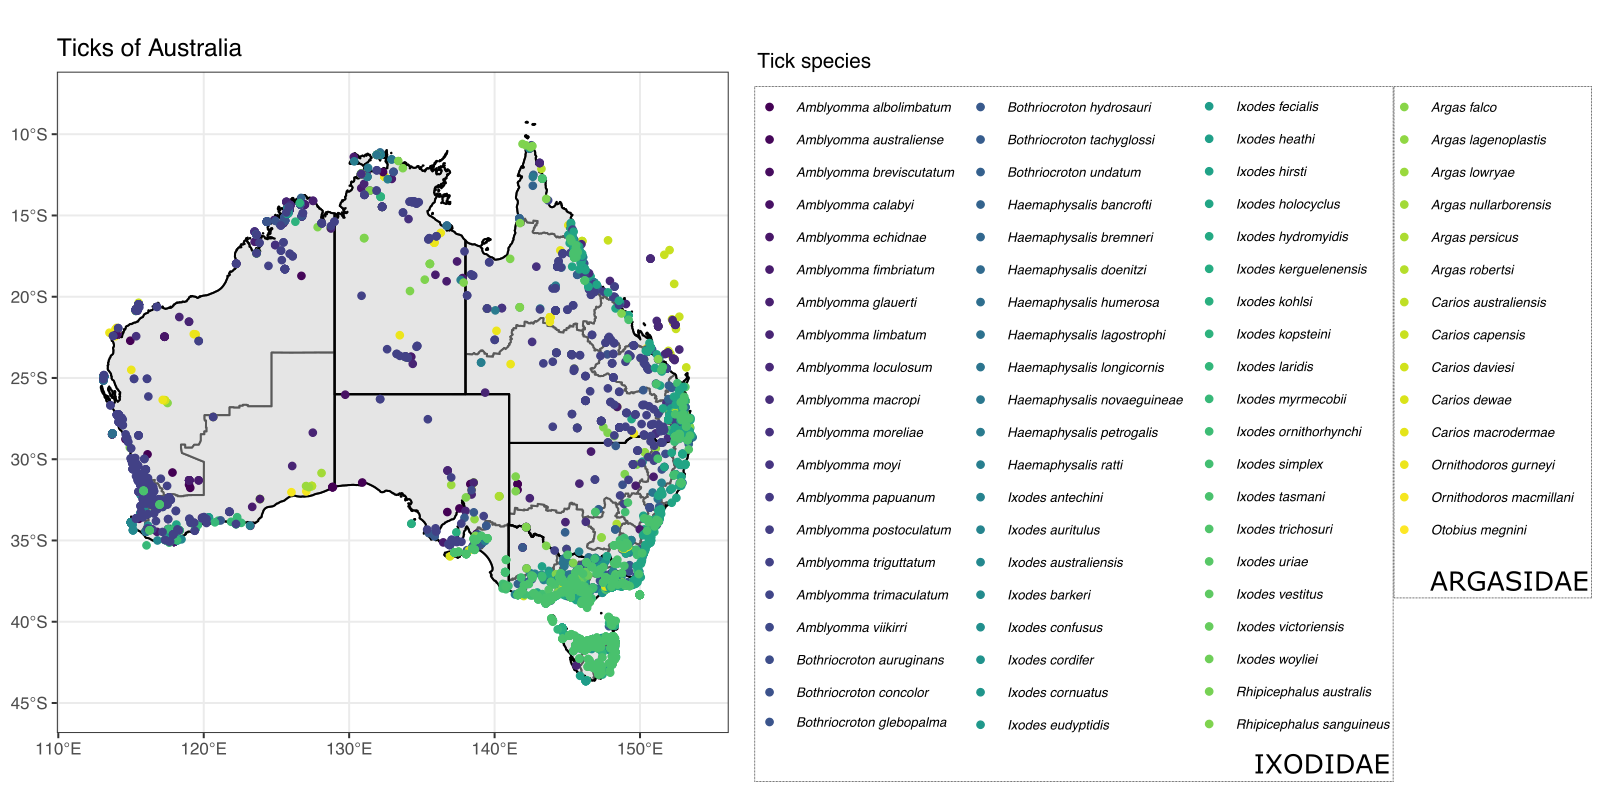
\includegraphics[width=0.95\linewidth]{figures/ms-figs/Ch2-mapallticks} \caption[Map of tick species present in Australia.]{Occurrence map of all known 74 species of ticks (Acari: Ixodida) present in Australia using record curated data.}\label{fig:F2mapall}
\end{figure}

\newpage

\begin{figure}
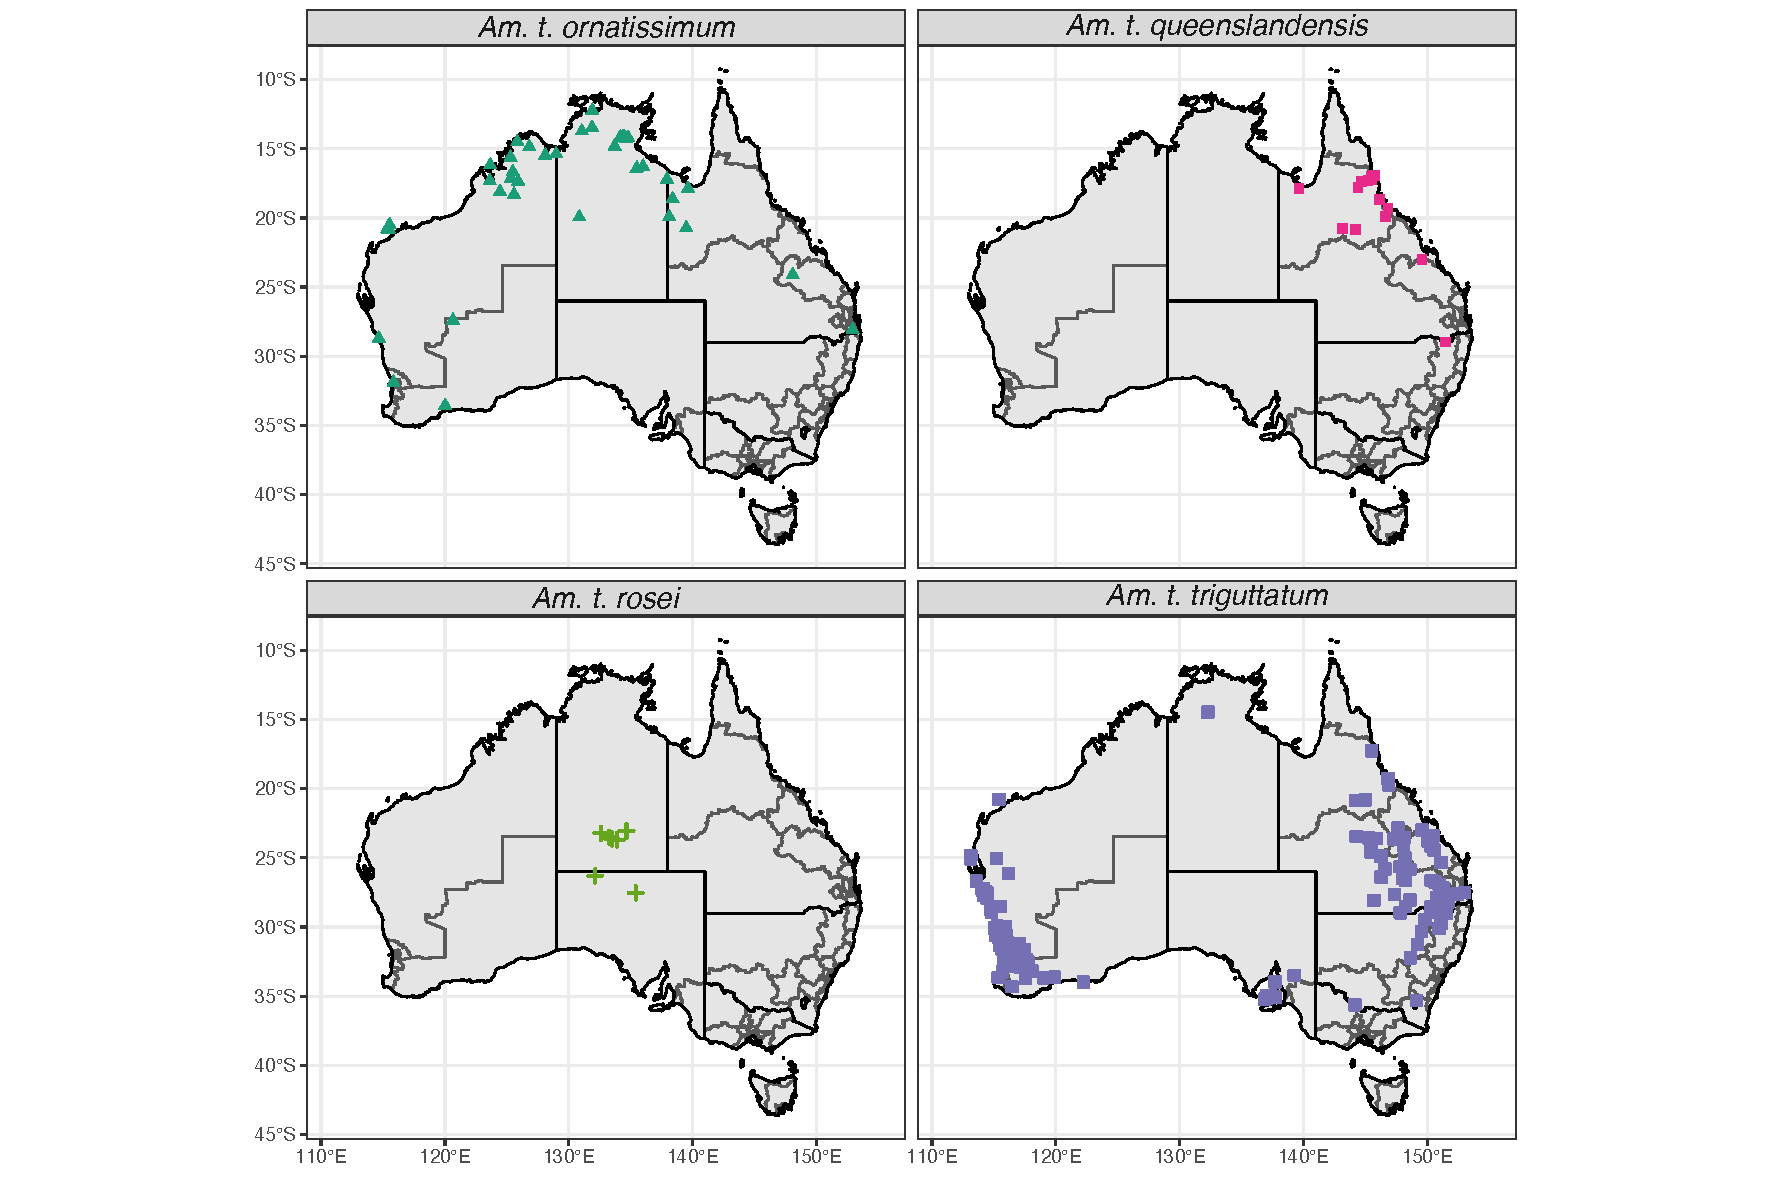
\includegraphics[width=0.95\linewidth]{figures/ms-figs/Ch2-amtrisubsp} \caption[Map of \textit{Am. triguttatum} subspecies.]{Occurrence map of the four \textit{Am. triguttatum} subspecies recorded in Australia. Only records with a valid subspecies identified are included.}\label{fig:F2atrigmapsubp}
\end{figure}

\newpage

\begin{figure}
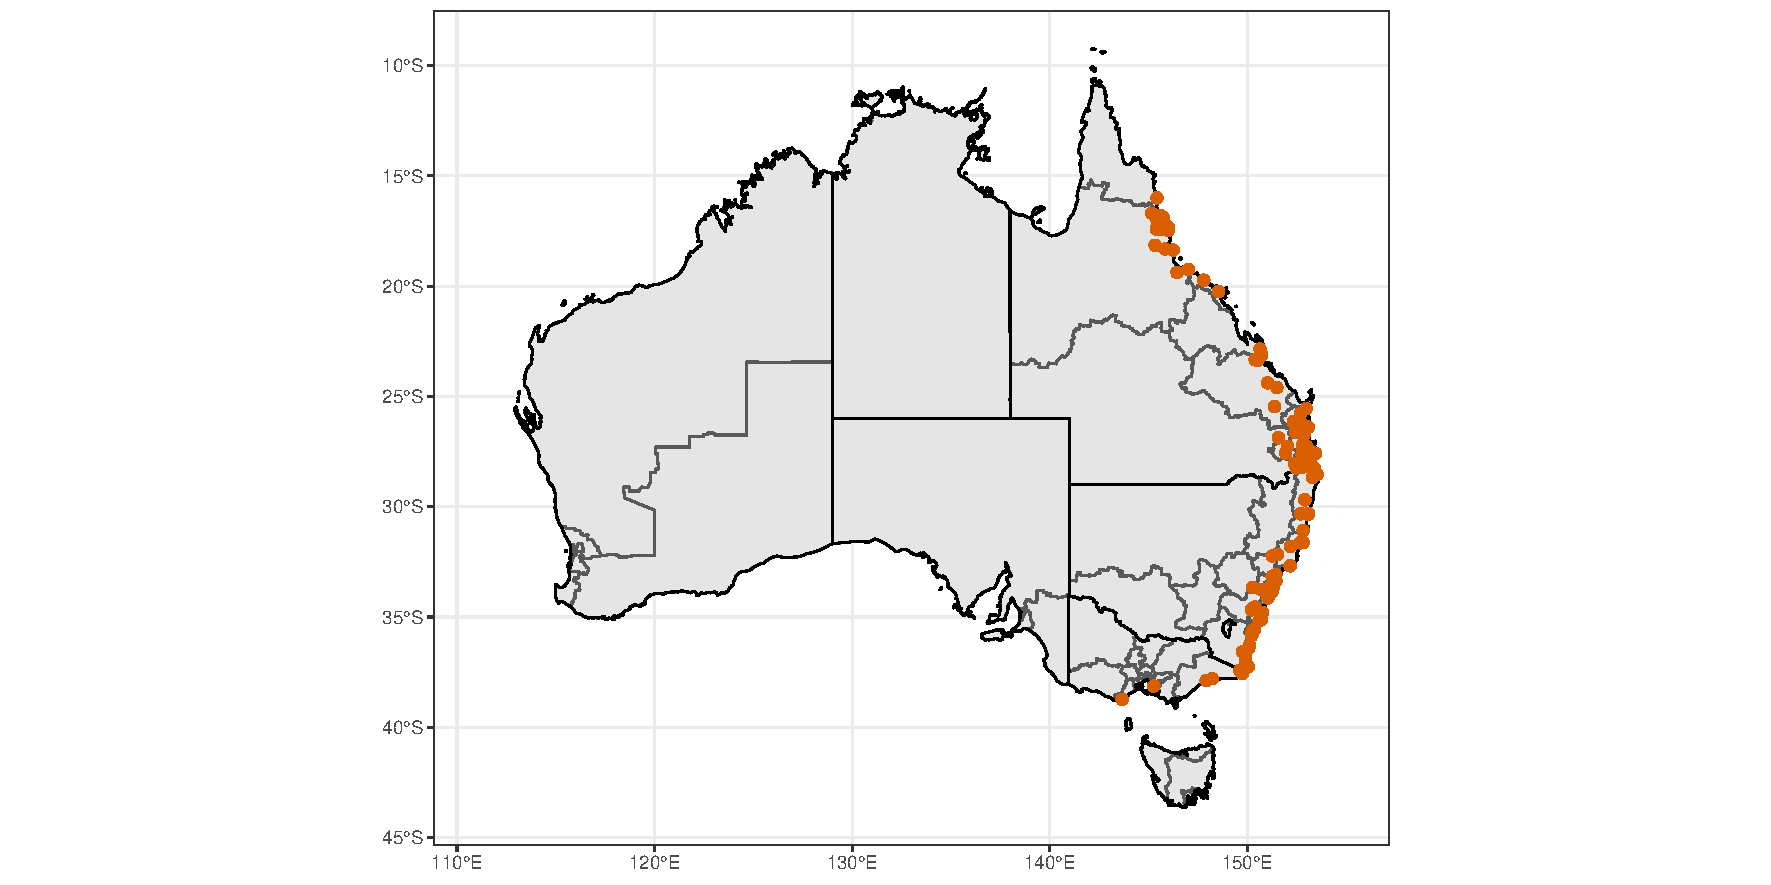
\includegraphics[width=0.95\linewidth]{figures/ms-figs/Ch2-map-ixhol} \caption[Map of \textit{Ix. holocyclus}.]{Occurrence map of \textit{Ix. holocyclus} records in Australia.}\label{fig:F2mapixhol}
\end{figure}

\begin{figure}
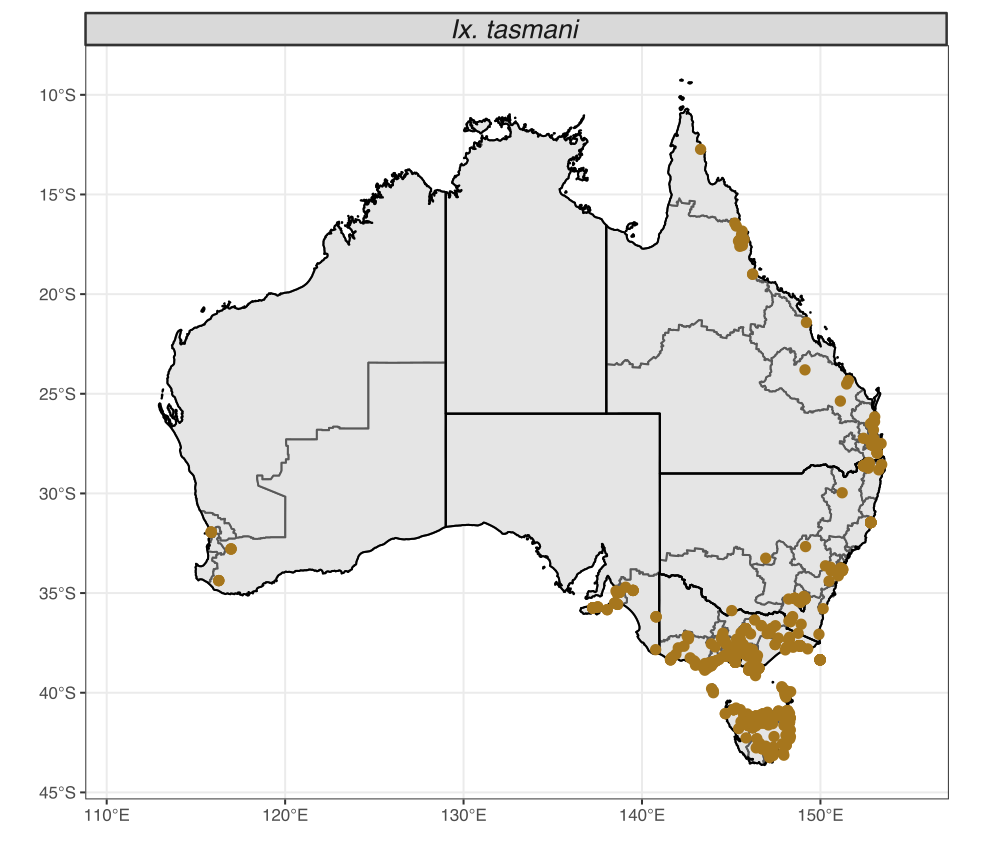
\includegraphics[width=0.95\linewidth]{figures/ms-figs/Ch2-map-ixtas} \caption[Map of \textit{Ix. tasmani}.]{Occurrence map of \textit{Ix. tasmani} records in Australia.}\label{fig:F2mapixtas}
\end{figure}

\newpage

\hypertarget{host-records-for-amblyomma-triguttatum}{%
\subsubsection{\texorpdfstring{Host records for \emph{Amblyomma triguttatum}}{Host records for Amblyomma triguttatum}}\label{host-records-for-amblyomma-triguttatum}}

A review of host records is available in table \ref{tab:T2atrig}, and identified the majority were from mammalian hosts.
Given its wide distribution among the mainland there are still many gaps in ecology and life history of \emph{Am. triguttatum}.
In comparison, similar tick species with a wide distribution in the northern hemisphere (e.g.~\emph{Ix. ricinus} and \emph{Ix. scapularis}) have been extensively studied \autocite{mihalcaRoleRodentsEcology2013,tietjenComparativeEvaluationNorthern2020}.

A recognised issue in distribution studies more broadly is the identification of areas that truly represent absence, as opposed to a lack of investigation.
\emph{Amblyomma triguttatum} is considered an exophilic tick and can be classified as a `hunter species'.
Observations by the authors note that species can be found readily in the environment where there is human activity.
In addition, \emph{Am. triguttatum} is a relatively large tick with unfed adults reaching 3--5 mm in size \autocite{robertsStatusMorphologicallyDivergent1962} and is readily identified on hosts.
With these factors in mind the authors consider that a lack of \emph{Am. triguttatum} identified is likely to be a true indicator of its absence, or at least of a small tick population size.
We note that in arid areas where flora and fauna studies persist, these have been good sources of records based on museum data obtained in the present study.
Therefore, until additional data is made available there is strong support that \emph{Am. triguttatum} persists in disjunct populations throughout Australia.

\textcite{waudbyHostsExoticOrnate2007} listed the domestic cat as a host and included a reference to \textcite{robertsAustralianTicks1970}, however after reviewing the suite of Roberts' tick publications, we have not been able to identify such a record.
We note however that a host record from a cat was included in additional data obtained by \textcite{waudbyHostsExoticOrnate2007}.

\clearpage

\begingroup\fontsize{8.5}{10.5}\selectfont

\begin{longtable}[t]{>{\raggedright\arraybackslash}p{3cm}>{}l>{\raggedright\arraybackslash}p{6cm}}
\caption[Host records for the ornate kangaroo tick.]{\label{tab:T2atrig}List of host records for \textit{Amblyomma triguttatum}. Abbreviations: Australian National Insect Collection (ANIC); Western Australian Museum (WAM). Where host records were ambiguous (e.g., kangaroo), taxa was assigned to the most commonly recorded species in the locality.}\\
\toprule
Host common name & Host scientific name & Reference\\
\midrule
\textbf{Class: Mammalia} & \em{\textbf{}} & \textbf{}\\
Monotremata & \em{} & \\
Platypus & \em{Ornithorhynchus anatinus} & Neumann 1901 - see Roberts (1962)\\
Short-beaked echidna & \em{Tachyglossus aculaetus} & Krige et al. 2017; ANIC\\
\textbf{Dasyuromorphia} & \em{\textbf{}} & \textbf{}\\
Numbat & \em{Myrmecobius fasciatus} & Calaby 1960; ANIC\\
\textbf{Peramelemorphia} & \em{\textbf{}} & \textbf{}\\
Greater Bilby & \em{Macrotis lagotis} & WAM\\
\textbf{Diprotodontia} & \em{\textbf{}} & \textbf{}\\
Koala & \em{Phascolarctos cinereus} & Barker \& Campelo unpublished - Barker and Walker 2014; Waudby et al. 2007; ANIC\\
Northern hairy-nosed wombat & \em{Lasiorhinus kreffti} & ANIC\\
Western ringtail possum & \em{Pseudocheirus occidentalis} & Clarke 2011\\
Common brushtail possum & \em{Trichosurus vulpecula} & Clarke 2011\\
Eastern grey kangaroo & \em{Macropus giganteus} & Pope et al. 1960; Roberts 1962, 1970; Guglielmone 1990; Cooper et al. 2013; ANIC\\
Western grey kangaroo & \em{Macropus fuliginosus} & Roberts 1962; Waudby et al. 2007; Loh et al. 2018; ANIC; WAM\\
Red kangaroo & \em{Macropus rufus} & Pope et al. 1960; Roberts 1962; Loh et al. 2018; ANIC; WAM\\
Tammar wallaby & \em{Notamacropus eugenii} & Waudby et al. 2007, 2018;ANIC\\
Bridled nail-tail wallaby & \em{Onychogalea frenata} & Turni and Smales 2001; ANIC\\
Swamp wallaby & \em{Wallabia bicolor} & Beveridge et al. 1985; Roberts 1962; ANIC\\
Agile wallaby & \em{Notamacropus agilis} & Roberts 1962; Speare et al. 1983; Cooper et al. 2013; ANIC\\
Black-striped wallaby & \em{Notamacropus dorsalis} & Roberts 1962; ANIC\\
Red-necked wallaby & \em{Notamacropus rufogriseus} & ANIC\\
Northern Nail-tail wallaby & \em{Onychogalea unguifera} & ANIC\\
Allied Rocky-wallaby & \em{Petrogale assimilis} & ANIC\\
Western brush wallaby & \em{Notamacropus irma} & ANIC\\
Unadorned Rock-wallaby & \em{Petrogale inornata} & ANIC\\
Whiptailed wallaby & \em{Notamacropus parryi} & Roberts 1970; ANIC\\
Spectacled Hare-wallaby & \em{Lagorchestes conspicillatus} & ANIC; WAM\\
Common wallaroo & \em{Osphranter robustus} & Roberts 1962; Cooper et al. 2013;  ANIC; WAM\\
Antilopine wallaroo & \em{Osphranter antilopinus} & ANIC\\
Northern bettong & \em{Bettongia tropica} & Barker \& Campelo unpublished - Barker and Walker 2014\\
Woylie & \em{Bettongia penicillata} & Kaewmongkol et al. 2011; Northover 2019; ANIC\\
Rufous bettong & \em{Aepyprymnus rufescens} & Cooper et al. 2013; ANIC\\
\textbf{Primates} & \em{\textbf{}} & \textbf{}\\
Human & \em{Homo sapiens} & Roberts 1962; Pearce and Grove 1987; McDiarmid et al. 2000; Andrews et al. 2007; Owen 2007; Gofton et al. 2015; ANIC; WAM\\
\textbf{Rodentia} & \em{\textbf{}} & \textbf{}\\
Black rat & \em{Rattus rattus} & Waudby et al. 2007\\
Laboratory / brown rat & \em{Rattus norvegicus} & Guglielmone and Moorhouse 1985(a)\\
\textbf{Lagomorpha} & \em{\textbf{}} & \textbf{}\\
Rabbit & \em{Oryctolagus cuniculus} & Roberts 1953(a); Guglielmone and Moorhouse 1985; Waudby et al. 2007; ANIC(a)\\
\textbf{Carnivora} & \em{\textbf{}} & \textbf{}\\
Dog & \em{Canis lupus familiaris} & Roberts 1962; Waudby et al. 2007; Andrews et al. 2007; Greay et al. 2016; ANIC; WAM\\
Cat & \em{Felis catus} & Waudby et al. 2007; WAM\\
\textbf{Perissodactyla} & \em{\textbf{}} & \textbf{}\\
Horse & \em{Equus caballus} & McCarthy 1960; Roberts 1962; Greay et al. 2016; Chalada et al. 2018; ANIC\\
\textbf{Artiodactyla} & \em{\textbf{}} & \textbf{}\\
Pig & \em{Sus scrofa} & Roberts 1962; Guglielmone 1990; Li et al. 2010; ANIC\\
Cattle & \em{Bos taurus} & Roberts 1962, 1970; ANIC\\
Swamp buffalo & \em{Babalus bubalis} & ANIC\\
Goat & \em{Capra hircus} & Pope et al. 1960\\
Domestic sheep & \em{Ovis aries} & Roberts 1962; ANIC; WAM\\
\textbf{Class: Aves} & \em{\textbf{}} & \textbf{}\\
Australian raven & \em{Corvus coronoides} & ANIC\\
Torresian crow & \em{Corvus orru} & ANIC\\
\textbf{Class: Reptilia} & \em{\textbf{}} & \textbf{}\\
Bobtail/sleepy lizard & \em{Tiliqua rugosa} & Waudby et al. 2007; Petney et al. 2008;\\
\bottomrule
\multicolumn{3}{l}{\rule{0pt}{1em}\textsuperscript{a} Host record reported from laboratory animals.}\\
\end{longtable}
\endgroup{}

\newpage

\hypertarget{molecular-barcodes-and-systematics}{%
\subsubsection{Molecular barcodes and Systematics}\label{molecular-barcodes-and-systematics}}

Molecular systematics has become the dominant method of species identification in disciplines including protozoology \autocite{maiaCommentsSystematicRevision2016,maslovRecentAdvancesTrypanosomatid2019} and microbiology \autocite{margosControversiesBacterialTaxonomy2019}.
However, for ectoparasites, including ticks, morphological tools remain the gold standard.
Therefore, the splitting of species based solely on molecular information without support of morphological features is unlikely to be useful to the field of tick taxonomy.
However, from an evolutionary perspective the molecular information generated here will assist in phylogenetic reconstructions and may assist in refining species boundaries.

New molecular barcodes generated in the present study are presented in Table \ref{tab:T2MLSTseqs} which include GenBank accession numbers.
An approach to tick taxonomy incorporating both traditional and new technologies is needed and consideration needs to be given to the broader impact of species nomenclature.
Particularly, for tick species of medical and veterinary importance, splitting species or a change of name can create confusion and wider uptake can be slow.
Compelling evidence for name changes is therefore needed before considering a new taxonomic nomenclature of these species.

The development of molecular information provides a fundamental tool to assist in species identification and systematics.
Unlike morphological descriptions and dichotomous keys, molecular barcodes are a characteristic of a species which is shared across all life stages.
As studies progress towards adapting an integrative approach in tick taxonomy \autocite{dantas-torresSpeciesConceptsWhat2018}, the use of molecular barcodes, as generated here, will be useful to identify characteristics used to deliminate species.

\textbf{\hl{High-throughput sequencing} sequencing}

\hl{High-throughput sequencing} sequencing targeting the 12S rDNA gene was successful at identifying tick species.
This included immature life stages where multiple specimens were pooled at the DNA extraction level.
Pooling of ticks (especially larvae and nymph stages) is implemented in many molecular studies of tick-borne pathogen or microbial characterisation to increase the throughput of samples \autocite{estrada-penaPitfallsTickTickBorne2021}.
The ability to deliminate species with a short sequence length (\textasciitilde{} 370 bp) make this high-throughput assay easily transferable to many short read sequence platforms.
The same extracted DNA or RNA used for pathogen detection and be used in the assay presented here to accurately determine species.
In particular, it is suited to the identification of immature tick life stages whose identity is ambiguous or where certain morphological features are missing or damaged, which prevent species-level identification.
An ability of the 12S rDNA gene to act as a barcoding gene for ticks has been identified in similar studies \autocite{lvAssessmentFourDNA2014,kandumaMitochondrialNuclearMultilocus2019}, and is shown by the level of phylogenetic separation among species shown in Figure \ref{fig:F2NGStree} (see list of accession numbers and species identification in Table \ref{tab:T2genbank}).
For example morphologically similar species, such as \emph{Ix. holocyclus} (OM830732) and \emph{Ix. cornuatus} (OM830728), can be distinguished easily as demonstrated in Figure \ref{fig:F2NGStree} (see also Table \ref{tab:T2genbank}).

\begin{figure}
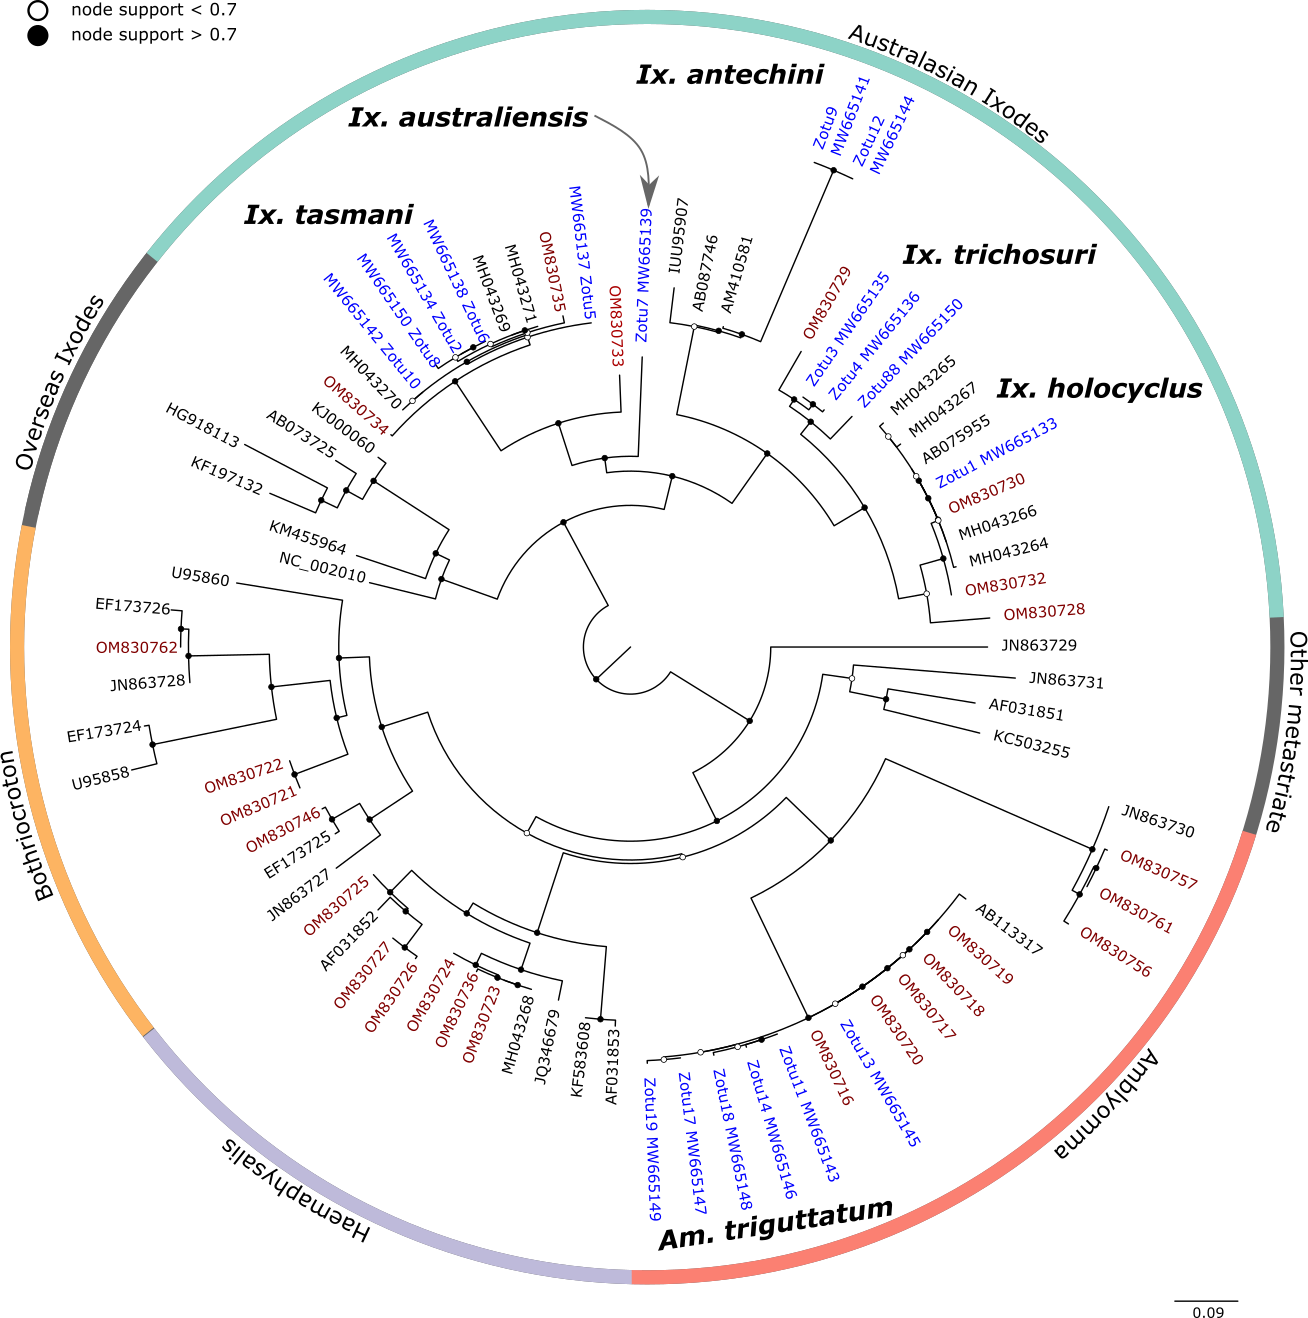
\includegraphics[width=0.95\linewidth]{figures/ms-figs/Ch2-12SNGStree} \caption[Phylogeny of tick species from wildlife.]{Maximum likelihood (ML) phylogenetic reconstruction of Ixodida ZOTUs based on a 377 bp alignment of the 12S rDNA gene Substitution model K3Pu +F + I + G4 with 10,000 replicates. Node values correspond to bootstrap support where values > 0.7 indicated by shaded circles. Number of substitutions per nucleotide position is represented by the scale bar. Sequences generated in the present study represented in blue (ZOTUs), and red (reference sequences).}\label{fig:F2NGStree}
\end{figure}

\hypertarget{limitations}{%
\subsection{Limitations}\label{limitations}}

The nature of using occurrence records to map distribution does have several limitations \autocite{fourcadeComparingSpeciesDistributions2016}.
However, as ticks are obligate blood feeders which require a host, the nature of their life history makes occurrence data more suitable to map distributions.
In particular, where tick species are aggressive human biting species, such as \emph{Am. triguttatum} \autocite{gravesTickborneInfectiousDiseases2017}, the absence of records is a useful indicator that the species is likely absent from that area.
Alternatively, low levels of human interactions in areas where the tick is present in the environment may also be responsible for absence of records.
A comprehensive search strategy was used and attempts were made to use a diverse range of sources (museum collections, public databases, grey literature etc.).
Therefore, we accept that it is possible that our occurrence maps may not represent the complete geographical distribution of all 74 tick species present in Australia.
Tick species distribution maps included a large portion of data based on historical identifications.
While every effort was made to ensure such records were from trusted sources, such as those identified by a suitability qualified person or collections from museum records, it is not possible to verify every single observation.
Where records outside of historic distributions or unusually sporadic data points were observed, efforts were made to verify specimen identification.

The generation of new molecular barcodes provided in the present study represents only a portion of the 74 tick species present in Australia.
Despite this, the authors feel this information is still valuable to researchers.
By making the molecular data public it will be of assistance to future researchers working towards genetic characterisation of ticks and be of use in phylogenetic reconstruction and taxonomic studies.

\hypertarget{conclusion}{%
\section{Conclusion}\label{conclusion}}

While the biology and natural history of ticks is understood in a broad context, much of this is based on data obtained from just a handful of species.
The most frequently incriminated human biting ticks in Europe and North America, \emph{Ixodes ricinus} and \emph{Ixodes scapularis}, are responsible for the majority of tick-borne infections in those continents \autocite{eisenBlackleggedTickIxodes2018,grayWhatWeStill2021}.
The life history and ecology of these tick species has been studied and provides important information needed to inform public health measures \autocite{grayWhatWeStill2021}.
In contrast few, if any, tick species in Australia have been studied to the same degree.

With rapid urbanization and the effects of climate change, the interface between humans and ticks is predicted to increase \autocite{gilbertImpactsClimateChange2021}.
Despite the well documented history of the discovery of Lyme disease in North America during the 1970's and 1980's \autocite{ostfeldFunctionBiodiversityEcology2000}, Australia continues to trail behind the rest of world with respect to knowledge about tick-borne diseases.
Without fundamental research into the natural history, ecology and molecular systematics of Australian ticks, the country is ill-equipped to understand the dynamics of potential tick-borne infections.

It is expected that the data presented from this research will provide the necessary foundations to further explore Australian tick systematics.
It is important that previous records are met with a healthy dose of criticism and work can begin towards a clearer understanding on Australian ticks.

\hypertarget{wildlife-bacteria}{%
\chapter{Microbiome of ticks and wildlife}\label{wildlife-bacteria}}

\chaptermark{Wildlife biome}

\includegraphics[width=0.95\linewidth]{front-and-back-matter/preface/Julimar_fieldwork}

\newpage

\hypertarget{preface-2}{%
\section*{Preface}\label{preface-2}}
\addcontentsline{toc}{section}{Preface}

\textbf{Attribution Statement}

The following chapter has been drafted in accordance with the journal \emph{Microbial Genomics}.

The following manuscript has been published: \textbf{Egan, S.}, Taylor, C., Banks, P., Northover, A., Alhstrom, L., Ryan, U., Irwin, P., and Oskam C. 2021. The bacterial biome of ticks and their wildlife hosts at the urban-wildland interface. \emph{Microbial Genomics}, \textbf{7}(12): 000730. DOI: \href{https://doi.org/10.1099/mgen.0.000730}{10.1099/mgen.0.000730}

The following authors contributed to this manuscript as outlined below\footnote{Contribution indicates the total involvement the author has had in this project. Placing an `X' in the remaining boxes indicates what aspect(s) of the project each author engaged in.}.

\begin{table}[!h]
\centering\begingroup\fontsize{7}{9}\selectfont

\begin{tabular}{lrllll}
\toprule
Authorship order & Contribution (\%) & Concept Development & Data Collection & Data Analysis & Draft\\
\midrule
\cellcolor{gray!6}{Siobhon L. Egan} & \cellcolor{gray!6}{70.0} & \cellcolor{gray!6}{X} & \cellcolor{gray!6}{X} & \cellcolor{gray!6}{X} & \cellcolor{gray!6}{X}\\
Casey L. Taylor & 6.0 &  & X &  & \\
\cellcolor{gray!6}{Peter B. Banks} & \cellcolor{gray!6}{2.5} & \cellcolor{gray!6}{X} & \cellcolor{gray!6}{} & \cellcolor{gray!6}{} & \cellcolor{gray!6}{}\\
Amy S. Northover & 2.5 &  & X &  & \\
\cellcolor{gray!6}{Liisa A. Ahlstrom} & \cellcolor{gray!6}{2.5} & \cellcolor{gray!6}{} & \cellcolor{gray!6}{X} & \cellcolor{gray!6}{} & \cellcolor{gray!6}{}\\
Una M. Ryan & 5.0 & X &  &  & \\
\cellcolor{gray!6}{Peter J. Irwin} & \cellcolor{gray!6}{5.0} & \cellcolor{gray!6}{X} & \cellcolor{gray!6}{} & \cellcolor{gray!6}{} & \cellcolor{gray!6}{}\\
Charlotte L. Oskam & 6.5 & X &  &  & \\
\bottomrule
\end{tabular}
\endgroup{}
\end{table}

By signing this document, the Candidate and Principal Supervisor acknowledge that the information provided is accurate and has been agreed to by all other authors.

\vspace{3mm}

\raggedright

\_\_\_\_\_\_\_\_\_\_\_\_\_\_\_\_\_\_ ~ ~ ~ \_\_\_\_\_\_\_\_\_\_\_\_\_\_\_\_\_\_\\
\hspace*{0.333em}\hspace*{0.333em}Candidate ~ ~ ~ ~ ~ ~ ~ ~ ~ ~ ~ ~ ~ ~ ~ ~ Principal Supervisor

\newpage

\textbf{Chapter linking statement:}
This chapter looks at the bacterial microbiome of wildlife samples. Using amplicon metabarcoding targeting the 16S rRNA gene to characterise the suite of bacteria in blood, tick and tissue samples. It provides an unbiased approach to investigate (i) what microbes are present in these wildlife samples and (ii) uncover overlap between sample types to provide insight into potential bacteria that maybe transmitted into wildlife which act as reservoir hosts. To obtain more detailed genetic information on `taxa of interest' further sequencing was performed. This chapter provides important insights into tick (and potentially other vector) associated microbes in Australia.

\vspace{5mm}

\textbf{Acknowledgment statement:}
This work was supported by resources provided by the Pawsey Supercomputing Centre with funding from the Australian Government and the Government of Western Australia.
We thank Dr David Chandler, Dr Christopher Noune and Dr Matthew Stevens at the Australian Genomics Research Facility for their assistance.
We thank the Department of Biodiversity, Conservation and Attractions staff for their invaluable assistance in Western Australian fieldwork, in particular Rebecca Kay, Douglas Giles and Hannah Kilian.
We also thank Jade Kelly and volunteers for assistance in fieldwork and sample collection.

\vspace{5mm}

\textbf{Funding statement:}
This study was part-funded by the Australian Research Council (LP160100200), Bayer HealthCare (Germany) and Bayer Australia.
S.L.E. was supported by an Australian Government Research Training Program (RTP) Scholarship.
C.L.T. was supported by a scholarship from the Northern Beaches Council.
This project was also part supported by The Holsworth Wildlife Research Endowment from The Ecological Society of Australia (awarded to S.L.E.) and the Paddy Pallin Science Grant from The Royal Zoological Society (awarded to C.L.T.).

\vspace{5mm}

\textbf{Data availability:}
Raw Illumina MiSeq data has been deposited in the European Nucleotide Archive under project number PRJEB46006 (\emph{16S rRNA} bacteria) and PRJEB46056 (\emph{12S rRNA} ticks).
Nucleotide data produced by Sanger sequencing has been submitted to NCBI GenBank nucleotide database under accession numbers MW633074, MW633076--MW633082, MW633160--MW633167.
A subset of representative zOTUs generated from tick \emph{12S rRNA} metabarcoding have been submitted to GenBank under accession numbers MW665133--MW665150.
Additional information is available within supplementary files including links to electronic files which have been deposited on FigShare \href{https://doi.org/10.6084/m9.figshare.14363627.v1}{repository}.
Code used for analysis and RData files used for bioinformatics and statistical analysis are available on GitHub repositories \href{https://github.com/siobhon-egan/wildlife-bacteria}{siobhon-egan/wildlife-bacteria} and \href{https://github.com/siobhon-egan/wildlife-ticks}{siobhon-egan/wildlife-ticks}.

\vspace{5mm}

\textbf{Animal ethics:} Murdoch University Animal Ethics Committee permit number R3026/18. Department of Biodiversity Conservation and Attractions permit numbers 2018/54B, 2018/55B, 2018/57D and 2017/30. University of Sydney Animal Ethics Committee Permit number 2018/1429.

\vspace{5mm}

\textbf{Author contributions::}
Conceptualization: S.L.E., U.M.R., P.J.I., C.L.O.
Data curation: S.L.E., C.L.T.
Formal Analysis: S.L.E.
Funding acquisition: S.L.E., C.L.T., P.B.B., L.A.A., U.M.R., P.J.I., C.L.O.
Investigation: S.L.E., C.L.T.
Methodology: S.L.E., C.L.T., A.S.N.
Project administration: P.J.I., C.L.O.
Resources: A.S.N., P.B.B., P.J.I., C.L.O.
Software: S.L.E.
Supervision: P.B.B., U.M.R., P.J.I., C.L.O.
Visualization: S.L.E.
Writing -- original draft: S.L.E.
Writing -- review \& editing: S.L.E., C.L.T., P.B.B., A.S.N., L.A.A., U.M.R., P.J.I., C.L.O.

\vspace{5mm}

\textbf{Keywords:} Tick, microbiome, wildlife, sylvatic cycle, tick-borne diseases,

\newpage

\hypertarget{abstract-1}{%
\section{Abstract}\label{abstract-1}}

Advances in sequencing technologies have revealed the complex and diverse microbial communities present in ticks (Ixodida).
As obligate blood feeding arthropods, ticks are responsible for a number of infectious diseases that can affect humans, livestock, domestic animals and wildlife.
While cases of human tick-borne diseases continue to increase in the northern hemisphere, there has been relatively little recognition of zoonotic tick-borne pathogens in Australia.
Over the past five years, studies using high-throughput sequencing technologies have shown that Australian ticks harbour unique and diverse bacterial communities.
In the present study, free-ranging wildlife (n = 203), representing ten mammal species, were sampled from urban and peri-urban areas in New South Wales (NSW), Queensland (QLD), and Western Australia (WA).
Bacterial metabarcoding targeting the 16S rRNA locus was used to characterise the microbiomes of three sample types collected from wildlife; blood, ticks and tissue samples.
Further sequence information was obtained for selected taxa of interest. Six tick species were identified from wildlife: \emph{Amblyomma triguttatum}, \emph{Ixodes antechini}, \emph{Ixodes australiensis}, \emph{Ixodes holocyclus}, \emph{Ixodes tasmani} and \emph{Ixodes trichosuri}.
Bacterial \emph{16S rRNA} metabarcoding was performed on 536 samples and 65 controls, generating over 100 million sequences.
Alpha diversity was significantly different between the three sample types, with tissue samples displaying the highest alpha diversity (P \textless{} 0.001).
\emph{Proteobacteria} was the most abundant taxon identified across all sample types (37.3\%).
Beta diversity analysis and ordination revealed little overlap between the three sample types (P \textless{} 0.001).
Taxa of interest included \emph{Anaplasmataceae}, \emph{Bartonella}, \emph{Borrelia}, \emph{Coxiellaceae}, \emph{Francisella}, \emph{Midichloria}, \emph{Mycoplasma} and \emph{Rickettsia.} \emph{Anaplasmataceae} bacteria were detected in 17.7\% (95/536) of samples and included \emph{Anaplasma}, \emph{Ehrlichia} and \emph{Neoehrlichia} species.
In samples from NSW `\emph{Ca}. Neoehrlichia australis', `\emph{Ca.}. Neoehrlichia arcana', \emph{Neoehrlichia} sp. and \emph{Ehrlichia} sp were identified.
A putative novel \emph{Ehrlichia} sp. was identified from WA and \emph{Anaplasma platys} was identified from QLD.
Nine rodent tissue samples were positive for a novel \emph{Borrelia} sp. which formed a phylogenetically distinct clade separate from the Lyme \emph{Borrelia} and relapsing fever groups.
This novel clade included recently identified rodent-associated \emph{Borrelia} genotypes, which were described from Spain and North America.
\emph{Bartonella} was identified in 12.9\% (69/536) of samples.
Over half of these positive samples were obtained from black rats (\emph{Rattus rattus}), and the dominant bacterial species identified were \emph{Bartonella coopersplainsensis} and \emph{Bartonella queenslandensis}.
The results from the present study show the value of using unbiased high throughput sequencing applied to samples collected from wildlife.
In addition to understanding the sylvatic cycle of known vector associated pathogens, surveillance work is important to ensure preparedness for potential zoonotic spillover events.

\hypertarget{introduction-1}{%
\section{Introduction}\label{introduction-1}}

Ticks carry a diverse range of infectious microbes such as viruses, piroplasms, spirochaetes and Rickettsiales \autocite{pfaffleEcologyTickborneDiseases2013}.
Globally recognised infectious human tick-borne diseases include Lyme borreliosis, ehrlichiosis, babesiosis, tick-borne encephalitis and Powassan viral disease.
Additionally, tick bite can cause reactions such as paralysis and anaphylaxis \autocite{vannunenAssociationTickBite2009}.
The incidence of tick-borne diseases \hl{in many parts of the word} is rapidly increasing in both prevalence and geographic distribution \autocite{madison-antenucciEmergingTickBorneDiseases2020}.
The sylvatic cycles of tick-borne pathogens in the northern hemisphere are generally well understood with respect to competent tick vectors and the reservoir hosts (e.g.~\emph{Babesia microti} \autocite{westbladeBabesiaMicrotiMice2017} and \emph{Borrelia burgdorferi} sensu lato \autocite{radolfTicksMiceMen2012}).
The value of wildlife health surveillance as a tool for the detection of emerging zoonotic infectious disease has been demonstrated in outbreaks historically, such as malaria \autocite{rondonPrevalencePlasmodiumParasites2019}, and more recently with SARS-CoV-2 \autocite{plowrightLandUseinducedSpillover2021}.

In Australia, three human tick-borne diseases are recognised; Queensland tick typhus (\emph{Rickettsia australis}), spotted fever (\emph{Rickettsia honei} subspp.) and Q fever (\emph{Coxiella burnetii}) \autocite{gravesTickborneInfectiousDiseases2017}.
Over the past decade there have been increasing concerns about unidentified tick-borne illness (syn. Lyme-like disease) in Australia \autocite{chaladaThereLymelikeDisease2016}, recently designated `Debilitating Symptom Complexes Attributed To Ticks' (DSCATT) by the Australian Government Department of Health \autocite{radcliffeGrowingEvidenceEmerging2016}.

Presently, 74 tick species have been described in Australia, including five introduced species \autocite{barkerIxodesBarkeriSp2019,evansAutomaticBarcodeGap2019}, of which 22 species have been identified biting humans \autocite{kwakFirstRecordsHuman2018}.
However, data show that \emph{Ixodes holocyclus} and \emph{Amblyomma triguttatum} account for \textgreater90\% of human tick bites, with the remainder of reports largely attributed to \emph{Ixodes tasmani}, \emph{Haemaphysalis bancrofti}, \emph{Haemaphysalis longicornis} and \emph{Bothriocroton hydrosauri} \autocite{kwakFirstRecordsHuman2018}.
Small to medium-sized mammals are important in maintaining these tick populations, in particular during the immature life stages \autocite{murdochEcologyCommonMarsupial2005,lydeckerPeriurbanBlackRats2019,taylorInvasiveRabbitsHost2020}.
While data on the incidence of human tick bites in Australia is limited, evidence suggests that tick bites are common in peri-urban areas, including residential yards (C Taylor, pers comms).

Over the past decade, due to new technologies there is mounting evidence that Australian ticks harbor a unique array of microbes \autocite{goftonInhibitionEndosymbiontCandidatus2015,eganBacterialCommunityProfiling2020}.
In addition to these molecular studies, more targeted screening of potential reservoirs such as dogs \autocite{irwinSearchingLymeBorreliosis2017} and sea bird ticks \autocite{moonAustralianPenguinTicks2018} have added to the growing body of evidence suggesting that human tick-borne pathogens described in the northern hemisphere are not endemic in Australia.
Some of the microbes that have recently been identified from Australian ticks however include new species of \emph{Borrelia} \autocite{lohMolecularCharacterizationCandidatus2017,panettaReptileassociatedBorreliaSpecies2017}, \emph{Ehrlichia} \autocite{goftonDetectionPhylogeneticCharacterisation2017}, \emph{Neoehrlichia} \autocite{goftonPhylogeneticCharacterisationTwo2016}, \emph{Babesia}, and \emph{Theileria} \autocite{greayEndemicExoticNovel2018,lohMolecularSurveillancePiroplasms2018} and several viruses \autocite{obrienDiscoveryNovelIflavirus2018,harveyExtensiveDiversityRNA2019}.
Little is known about the sylvatic life cycle of these microbes or their wildlife species reservoir hosts. Even for the few tick-borne pathogens recognised in Australia (e.g.~\emph{Rickettsia} spp.), much of this information remains elusive.

For a tick-borne disease to become established it requires a temporal and spatial overlap between the microbe (pathogens), competent vector tick(s), and one or more vertebrate reservoir hosts.
In the northern hemisphere studies have shown that there are important differences in the role of host species in maintaining the sylvatic cycle of tick-borne pathogens \autocite{leviQuantifyingDilutionAmplification2016,huangHighBurdensIxodes2019,stewartmerrillMechanisticUnderstandingCompetence2020}.
Broadly, reservoir hosts can be classified as amplification and dilution hosts. Amplification hosts, in most cases, are small mammals that host immature ticks (larvae or nymph stages) and increase the environmental density of infected nymphs \autocite{leviQuantifyingDilutionAmplification2016}.
In contrast, dilution hosts are inefficient reservoirs of the microbial agent(s) \autocite{takumiImpactVertebrateCommunities2019,ginsbergWhyLymeDisease2021}.
An additional factor is the role of hosts throughout the tick life cycle.
Larger animals are considered important in maintaining adult stages of the tick; white-tailed deer (\emph{Odocoileus virginianus}) and \emph{Ixodes scapularis} \autocite{ostfeldTickborneDiseaseRisk2018} for example.
In the Australian context it is generally assumed that small mammals such as bandicoots, possums and rodents are likely reservoirs for tick-associated microbes.
In turn, larger mammals such as kangaroos and wallabies may then play an important role in maintaining tick populations, filling a similar ecological niche as deer in the northern hemisphere.
While studies have used molecular tools to investigate microbes present within ticks in Australia \autocite{goftonPhylogeneticCharacterisationTwo2016,lohMolecularSurveillancePiroplasms2018,moonAustralianPenguinTicks2018}, very little research has been conducted at the vertebrate host level to further elucidate the sylvatic cycle of tick transmitted bacteria.
Bacterial amplicon sequencing is valuable in the setting of wildlife epidemiology surveys where investigations are not confined to existing presumptions of microbes \autocite{galan16SRRNAAmplicon2016}, however such studies of the ticks alone, without concurrent analysis of vertebrate host tissues, cannot distinguish infectious components of the tick's total microbiome from those that are non-transmissible.\\
Therefore, the search for tick-associated microbes in vertebrate host(s) is the next logical piece of information required to untangle the complex dynamics of tick-borne pathogens.
In addition to novel pathogen discovery, high throughput sequencing technologies applied concomitantly to tick and vertebrate host tissues can provide insights into the dynamics of microbial epidemiology and interactions within landscapes \autocite{titcombHighThroughputSequencingUnderstanding2019}.
Identification of microbes may inform our understanding of the tick-borne disease risk and potential differences among temporal and spatial gradients.

The present study used metabarcoding to explore the bacterial communities present in Australian wildlife and their ticks, with a focus on bacteria related to known (vector-borne) pathogens, to provide insights into the sylvatic life cycle of tick associated organisms.
This research was conducted in an ecological zone referred to as the urban-wildland interface, where there is a transition between wilderness and land developed by human activity -- an area where a built environment meets or intermingles with a natural environment.

\hypertarget{methods-1}{%
\section{Methods}\label{methods-1}}

\hypertarget{study-sites-and-sample-collection}{%
\subsection{Study sites and sample collection}\label{study-sites-and-sample-collection}}

\textbf{Small mammal trapping}

Small mammal trapping was performed at various sites in Perth, Western Australia and Sydney, New South Wales (Figure \ref{fig:F3map}).
Each site was targeted in urban and peri-urban areas to reflect the urban-wildland interface.
Elliot and cage traps were set and baited with universal bait (rolled oats, peanut butter and sardines).
Traps were set at dusk and cleared at sunrise over three or four consecutive nights. To ensure a comprehensive assessment and sampling, target mammals were briefly anaesthetised in the field using isoflurane (I.S.O. 1mL/mL) vaporised in medical oxygen.
Animals were weighed and examined systematically for ectoparasites.
Up to 1 mL of blood was collected from either the caudal (tail) vein, femoral vein or ear capillary and stored in Mini Collect EDTA tubes.
If practical, a 2 mm punch biopsy was taken at the tick bite site; where possible, a biopsy was taken from the ear and stored in RNAlater or 80\% ethanol.
Animals were systematically examined for ectoparasites which were removed and stored in 80\% ethanol.
Animals were recovered from anaesthesia by providing medical oxygen, and once fully alert were released at trap point.
An individual mark was applied to identify animals using either a microchip administered subcutaneously or a unique patch of hair was removed.
The number of animals and samples analysed, and locations from the present study are available in Table \ref{tab:T3hosts} and Figure \ref{fig:F3map} respectively.

\textbf{Opportunistic collection}

In a small number of cases, animal carcasses were also obtained opportunistically. These specimens were collected through incidental findings during fieldwork or from situations where animals were humanely euthanised in accordance with animal ethics and state and federal guidelines.

\textbf{Tick identification}

Ticks were collected and stored in tubes containing 70--90\% ethanol. Samples were visualised using an Olympus SZ61 stereomicroscope (Olympus, Centre Valley, PA, United States) with an external Schott KL 1500 LED (Schott AG Mainz, Germany) light source.
Photographs of tick specimens were taken using an Olympus SC30 digital camera (Olympus, Centre Valley, PA, United States) and analysis getIT software (Olympus, Centre Valley, PA, United States).
Instar, sex and species was identified using a combination of available morphological keys and species descriptions \autocite{robertsAustralianTicks1970,jacksonMorphologicalComparisonAdult2002,laanObservationsBiologyDistribution2011,barkerTicksAustraliaSpecies2014,kwakPhylogeneticAnalysisAustralian2017}.

\begin{table}

\caption[Host sample numbers for bacterial microbiome study.]{\label{tab:T3hosts}Animal sampling numbers for bacterial microbiome sequencing. Number of individual animals (\textit{n}) by host species with number of genomic DNA samples analysed in parentheses.}
\centering
\fontsize{8.5}{10.5}\selectfont
\begin{tabular}[t]{l>{}lcccc}
\toprule
Common name & Scientific name & n (individuals) & Blood & Tick & Tissue\\
\midrule
Black rat & \em{Rattus rattus} & 88 & 68 (84) & 54 (79) & 71 (80)\\
Brown antechinus & \em{Antechinus stuartii} & 5 & 0 (0) & 4 (6) & 2 (2)\\
Brush tail possum & \em{Trichosurus vulpecula} & 27 & 18 (21) & 15 (33) & 16 (20)\\
Bush rat & \em{Rattus fuscipes} & 3 & 2 (2) & 3 (4) & 3 (3)\\
Chuditch & \em{Dasyurus geoffroii} & 22 & 22 (24) & 1 (1) & 9 (9)\\
Deer & \em{Rusa timorensis} & 3 & 0 (0) & 0 (0) & 3 (6)\\
Long-nosed bandicoot & \em{Perameles nasuta} & 44 & 20 (25) & 31 (60) & 40 (44)\\
Quenda & \em{Isoodon fusciventer} & 2 & 1 (1) & 2 (2) & 0 (0)\\
Rabbit & \em{Oryctolagus cuniculus} & 7 & 0 (0) & 7 (20) & 7 (7)\\
Swamp rat & \em{Rattus lutreolus} & 2 & 1 (1) & 0 (0) & 1 (1)\\
\textbf{Total} & \em{\textbf{}} & \textbf{203} & \textbf{132 (159)} & \textbf{117 (205)} & \textbf{152 (172)}\\
\bottomrule
\end{tabular}
\end{table}

\begin{figure}
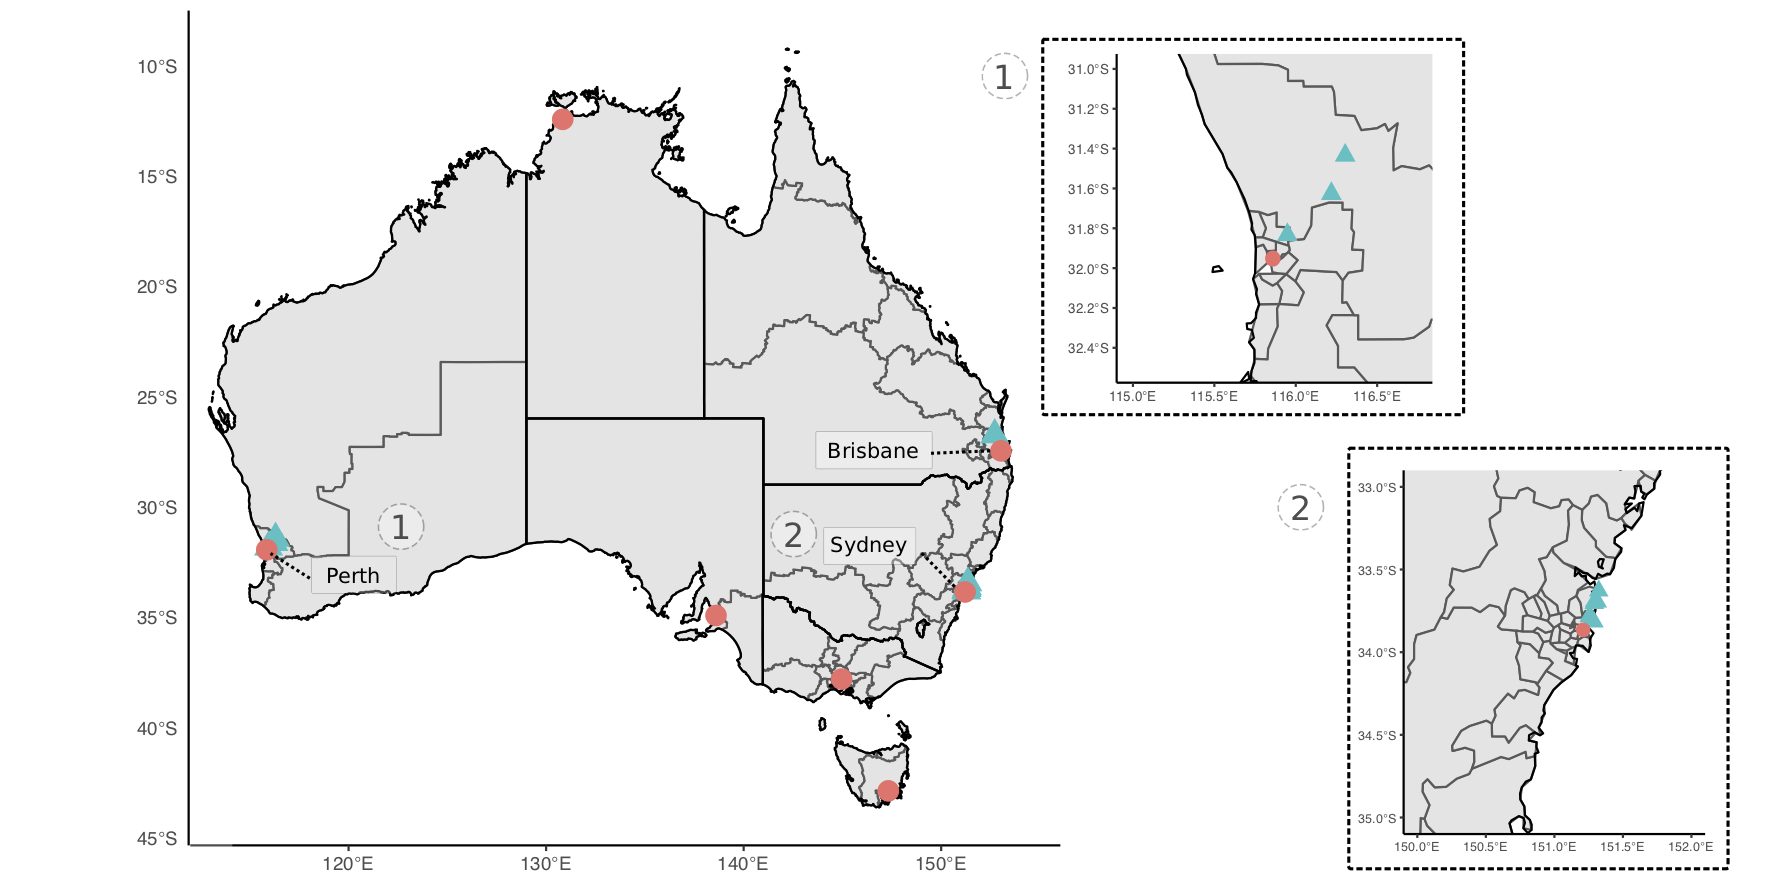
\includegraphics[width=0.95\linewidth]{figures/ms-figs/Ch3-map} \caption[Map of study sites for wildlife samples.]{Map of study sites for collection of wildlife samples used in bacterial profiling. Sampling sites denoted by blue triangles and capital cities by pink circles (for geographical reference). Insert maps of sites in (1) Perth, Western Australia and (2) Sydney, New South Wales.}\label{fig:F3map}
\end{figure}

\hypertarget{dna-extractions}{%
\subsection{DNA Extractions}\label{dna-extractions}}

Total genomic DNA (gDNA) was extracted from 200 \(\mu\)L of blood using a MasterPure DNA purification kit (Epicentre\textregistered Biotechnologies, Madison, Wisconsin, U.S.A) following the manufacturer's recommendations. Where 200 \(\mu\)L of blood was not available, sterile DNA free phosphate-buffered saline (PBS) was used to make samples up to 200 \(\mu\)L.
Genomic DNA was eluted in 30--40 \(\mu\)L of TE buffer and stored at -20\(^\circ\)C until further processing.

Tissue samples (skin and spleen) were first rinsed in sterile, DNA-free PBS and cut into small pieces (\textless1-2 mm) using a sterile scalpel blade.
Samples were homogenised in 180 \(\mu\)L of buffer ATL and 20 \(\mu\)L of proteinase K was added and incubated at 56\(^\circ\)C for \textasciitilde{} 16 hours. gDNA was extracted using the QIAamp DNA Mini Kit (QIAGEN, Germany) following the manufacturer's protocols with the exception that final elution volume was decreased to 40--50 \(\mu\)L to increase gDNA yield.

Once ticks were identified, they were surface-sterilised by washing in 10 \% hypochlorite solution, rinsed in 70 \% ethanol and DNA-free PBS, and then air-dried.
Genomic DNA was extracted using the DNeasy Blood and Tissue kit (QIAGEN, Germany) for adults, or the QIAamp DNA Mini Kit (QIAGEN, Germany) for nymphs and larvae.
Due to the large number of immature tick stages collected from some animals and the expected low DNA yield, up to 5 specimens were pooled for extraction based on host, instar, engorgement status and species identification as determined by morphological methods.
Ticks were placed in a 2 mL safe lock Eppendorf tube with a 5 mm steel bead, frozen in liquid nitrogen for 1 min and homogenised by shaking at 40 Hz in a Tissue Lyser LT (QIAGEN, Germany).
Final elution of DNA was adjusted according to tick size, between 30--150 \(\mu\)L of AE buffer was added to the silicon membrane.

Extraction controls (EXBs) consisting of 200 \(\mu\)L sterile DNA-free PBS were included randomly in each extraction batch (total EXBs = 34).
Blood and tissue samples were extracted in a separate laboratory, away from where ticks were processed, to avoid cross-contamination between sample types. Sterile procedures were followed throughout the laboratory process.

\hypertarget{metabarcoding-sequencing}{%
\subsection{Metabarcoding sequencing}\label{metabarcoding-sequencing}}

A high-throughput metabarcoding approach was used to sequence samples using the Illumina MiSeq platform. Libraries were built following the 16S Metagenomic Sequencing Library Preparation (Illumina Part \# 15044223 Rev.~B), with amplicon PCR primers containing Illumina MiSeq adapter sequences (Table \ref{tab:T32}).
A total of 536 samples from 203 individuals (159 blood, 205 tick pools, and 172 tissue samples) underwent bacterial profiling.

Bacterial \emph{16S rRNA} libraries were built targeting the 16S hypervariable region 1-2 using primers 27F-Y and 338R \autocite{goftonInhibitionEndosymbiontCandidatus2015}.
Reactions were carried out in 25 \(\mu\)L volumes each containing: 1X buffer (KAPA Biosystems, South Africa), 1.5 mM MgCl\textsubscript{2}, 0.4 mg/mL of bovine serum albumin (Fisher Biotech), 0.4 \(\mu\)M of each primer, 0.25 mM of each dNTP, 0.5 U of Taq (KAPA Biosystems, South Africa) and 2 \(\mu\)L of gDNA.
Thermal cycling conditions were as follows; 95\(^\circ\)C for 5 mins, followed by 35 cycles of 95\(^\circ\)C for 30 secs, 55\(^\circ\)C for 30 secs, 72\(^\circ\)C for 45 secs; and a final extension of 72\(^\circ\)C for 5 mins.
For a subset of samples where microbes of interest were identified after initial screening at the v1-2 hypervariable region, additional bacterial \emph{16S rRNA} libraries targeting the v3-4 hypervariable region were also prepared.
Primers 338F and 806R were used to target an \textasciitilde450 bp product.
Reactions and thermal cycling conditions were carried out as per the 27F-Y / 338R assay, except for an increased concentration of MgCl\textsubscript{2} to 2.0 mM.

To confirm morphological identification tick gDNA underwent amplicon metabarcoding approach targeting the 12S rDNA gene.
Pan-Ixodida primers T1B/T2A \autocite{beatiAnalysisSystematicRelationships2001} were used to amplify an \textasciitilde370 bp product of the 12S rDNA gene
Reactions were carried out as per the bacteria 27F-Y / 338R assay, except only 1 \(\mu\)M of tick gDNA template was added.
Thermal cycling conditions were as follows; 95\(^\circ\)C for 5 mins, followed by 5 cycles of 95\(^\circ\)C for 15 secs, 51\(^\circ\)C for 30 secs, 68\(^\circ\)C for 30 secs; 25 cycles of 95\(^\circ\)C for 30 secs, 53\(^\circ\)C for 30 secs, 72\(^\circ\)C for 1 min; and a final extension of 72\(^\circ\)C for 5 mins.

Amplicon PCR products were then indexed using the Nextera XT DNA library preparation kit in 25 \(\mu\)L volumes following the manufacturer's recommendations.
All PCRs included no-template controls (NTC; total = 31) during each reaction set up and PCRs were performed under strict laboratory conditions.
Amplicons were then dual-indexed using the Nextera XT index kit.
Reactions were performed in 25 \(\mu\)L volumes following manufacturers recommendations.
Libraries were purified with Axygen PCR clean up beads and quantified using Qubit High Sensitivity dsDNA assay kit (Thermo Fisher Scientific, Waltham, MA, USA) and pooled in equimolar amounts.
Libraries were shipped to the Australian Genomic Research Facility (Melbourne, Australia) for final QC and sequenced on an Illumina MiSeq using v2 chemistry (2 x 250 paired-end).



\begin{table}

\caption[Primers used for bacteria detection in samples from ticks and wildlife.]{\label{tab:T32}List of sequencing used for metabarcoding and target PCRs to screen blood, tissue and tick samples for bacteria. References \textbf{1.} Gofton et al. \autocite*{goftonInhibitionEndosymbiontCandidatus2015}, \textbf{2.} Turner et al. \autocite*{turnerInvestigatingDeepPhylogenetic1999}, \textbf{3.} Lopez et al. \autocite*{lopezDesignEvaluationPCR2003}, \textbf{4.} Caporaso et al. \autocite*{caporasoGlobalPatterns16S2011}, \textbf{5.} Beard et al. \autocite*{beardBartonellaSppFeral2011}, \textbf{6.} Anderson et al. \autocite*{andersonEhrlichiaChaffeensisNew1991}, \textbf{7.} Paddock et al. \autocite*{paddockIsolationCharacterisationEhrlichia1997}, \textbf{8.} Kawahara et al. \autocite*{kawaharaUltrastructurePhylogeneticAnalysis2004}, \textbf{9.} Beati and Keirans 2001 \autocite*{beatiAnalysisSystematicRelationships2001}.}
\centering
\fontsize{8.5}{10.5}\selectfont
\begin{tabular}[t]{lll}
\toprule
Primer & Sequence (5'-3') & Ref\\
\midrule
\textbf{Bacteria 16S rRNA} & \textbf{} & \textbf{}\\
27F-Y & AGAGTTTGATCCTGGCTYAG & 1\\
338R & TGCTGCCTCCCGTAGGAGT & 2\\
338F & ACTCCTACGGGAGGCAGCAG & 3\\
806R & GGACTACHVGGGTWTCTAAT & 4\\
\textbf{Bartonella 16S rRNA/ ITS} & \textbf{} & \textbf{}\\
438s & GGTTTTCCGGTTTATCCCGGAGGGC & 5\\
1100as & GAACCGACGACCCCCTGCTTGCAAAGC & 5\\
\textbf{Anaplasmataceae 16S rRNA} & \textbf{} & \textbf{}\\
EC9 & TACCTTGTTACGACTT & 6\\
EC12 & TGATCCTGGCTCAGAACGAACG & 7\\
A171a & GCGGCAAGCCTCCCACAT & 8\\
IS58-1345r & CACCAGCTTCGAGTTAAACC & 8\\
\bottomrule
\end{tabular}
\end{table}

\hypertarget{bioinformatics}{%
\subsection{Bioinformatics}\label{bioinformatics}}

Metabarcoding \emph{16S rRNA} sequence data was analysed using Quantitative Insights into Microbial Ecology (QIIME 2 2020.11) \autocite{bolyenReproducibleInteractiveScalable2019}. Briefly, raw sequences were demultiplexed and quality filtered using the q2-demux plugin, followed by denoising using DADA2 (via q2-dada2) \autocite{callahanDADA2HighresolutionSample2016} resulting in amplicon sequence variations (ASVs) (i.e.~100\% identical operational taxonomic units or OTUs \autocite{callahanExactSequenceVariants2017}).
Bacterial data taxonomy was assigned to ASVs using the q2‐feature‐classifier \autocite{bokulichOptimizingTaxonomicClassification2018} classify‐sklearn naive Bayes taxonomy classifier against the SILVA database \autocite{quastSILVARibosomalRNA2013} (release 132).
Taxonomic assignments were confirmed using BLAST analysis (BLASTN 2.11.0+ \autocite{zhangGreedyAlgorithmAligning2000,morgulisDatabaseIndexingProduction2008}) against the NCBI nucleotide collection (nt) database (accessed January 2021).
Taxonomic lineage was then retrieved from NCBI taxonomy database using TaxonKit \autocite{weissHostReproductiveCycle2021} and adjusted to the lowest common ancestor based on percentage identity and e-value score.

Tick \emph{12S rDNA} metabarcoding sequences generated were analysed USEARCH v11 \autocite{edgarSearchClusteringOrders2010} pipeline.
Briefly paired end reads were merged and sequences matching forward and reverse primers were retrieved (max number of mismatches = 2).
Sequences were then quality filtered and singletons were removed.
The unoise3 \autocite{edgarUNOISE2ImprovedErrorcorrection2016} algorithm was used to perform denoising (error-correction) and generate zero-radius taxonomic units (zOTUs) equivalent to amplicon sequence variants (ASVs).
Taxonomy was assigned using BLAST analysis and lineage retrieved as outlined above for \emph{16S rRNA} metabarcoding.

Data visualization and statistical analysis was performed in RStudio (v1.4) with R version 4.0.2. The main R packages used were ampvis2 v2.6.7, phyloseq v1.34.0, microbiomeutilities v1.00.12 and vegan v2.5-7. The R package decontam v1.10.0 \autocite{davisSimpleStatisticalIdentification2018} was used to inspect data for cross-contamination and cross-talk between samples and to establish read cut-off thresholds (prevalence threshold = 0.05). Identified contaminant ASVs (n = 104), controls samples (n = 65) and sequence values \textless{} 100 were removed. Rarefaction curves were generated using a step size of 100. Alpha diversity was measured using four indexes (number of observed ASVs, Chao1, Shannon and invSimpson) and statistical analysis was calculated using Wilcoxon pairwise test (non-parametric) between sample types (blood, tick and tissue). Heatmaps were generated using ampvis2, where data was first aggregated to family level and transformed to relative abundance.

Constrained ordination analysis was performed using two methods, canonical correspondence analysis and redundancy analysis (constrained principal component analysis), to investigate the relationships between sample types.
Prior to the analysis ASVs \textless{} 0.1 relative abundance and samples with \textless{} 1000 sequences were removed.
Data was first transformed using the Hellinger transformation and distance was measured using the Bray-Curtis method.
Beta diversity statistical analysis was performed using analysis of variance (ANOVA) and permutational multivariate analysis of variance (PERMANOVA) (999 permutations) via the adonis function in the vegan package \autocite{oksanenVeganCommunityEcology2020}, (Hellinger transformation and Bray-Curtis distance measure), the F statistic and P value are presented (full statistical output available in Supplementary Material \ref{ch3stats}).
Hierarchical cluster analysis was performed using euclidean distance measure (average), where data was first transformed using Hellinger transformation.

The composition for taxa of interest was aggregated to family level and compared between the three sample types.
Taxa of interest are defined as bacteria related to known pathogens associated with ticks and other vectors described globally, as outlined in Egan et al. \autocite*{eganBacterialCommunityProfiling2020}.
Statistical analysis was performed using the Wilcoxon pairwise test (non-parametric).
To identify shared ASVs (i.e.~core microbiome) between sample types and species, data was transformed to relative abundance and assigned to best taxonomic hit using the microbiomeutilities R package.
Similarities of the core microbiome between the three sample types were investigated using thresholds of abundance and prevalence between 0.0001---0.001 and 0.001---0.05 respectively.
For subsequent comparisons of the core microbiome between host and tick species, abundance and prevalence levels were set at 0.001 and 0.05 respectively.
Prevalence data for taxa of interest is presented for samples based on \emph{16S rRNA} metabarcoding. Where ticks have been pooled, prevalence is reported based on minimum infection rates (i.e.~assumes only one positive tick in each pool) \autocite{estrada-penaPitfallsTickTickBorne2021}.

Scripts for data analysis are available at \href{https://github.com/siobhon-egan/wildlife-bacteria}{siobhon-egan/wildlife-bacteria} and \href{https://github.com/siobhon-egan/wildlife-ticks}{siobhon-egan/wildlife-ticks} and raw Illumina MiSeq data has been deposited in the European Nucleotide Archive under project accession number PRJEB46056 (\emph{16S rRNA} bacteria) and PRJEB46056 (\emph{12S rRNA} ticks).

\hypertarget{target-pcrs}{%
\subsection{Target PCRs}\label{target-pcrs}}

A nested PCR was used to amplify \textasciitilde1.4 kb fragment of 16S rRNA gene for \emph{Neoehrlichia} and \emph{Ehrlichia.}
Amplicon PCRs were carried out in 25 \(\mu\)L reactions each containing: 1X buffer (KAPA Biosystems, South Africa), 2.5 mM MgCl\textsubscript{2}, 0.4 \(\mu\)M of each primer, 0.25 mM of each dNTP, 0.5 U of Taq (KAPA Biosystems, South Africa) and 2 \(\mu\)L of gDNA or 1 \(\mu\)L of primary product.
Thermal cycling conditions were as follows; 95\(^\circ\)C for 3 mins, followed by 40 cycles of 95\(^\circ\)C for 30 secs, 48\(^\circ\)C (primary) or 54\(^\circ\)C (secondary) for 1 min, 72\(^\circ\)C for 2 mins; and a final extension of 72\(^\circ\)C for 5 mins.

For \emph{Bartonella}, a PCR was used to amplify a \textasciitilde370-450 bp fragment of the \emph{16S rRNA} - \emph{23S internal transcribed spacer} (ITS) region.
Amplicon PCRs were carried out in 25 \(\mu\)L reactions each containing: 1X buffer (KAPA Biosystems, South Africa), 2.0 mM MgCl\textsubscript{2}, 0.4 \(\mu\)M of each primer, 0.25 mM of each dNTP, 0.5 U of Taq (KAPA Biosystems, South Africa) and 2 \(\mu\)L of gDNA.
Thermal cycling conditions were as follows; 95\(^\circ\)C for 3 mins, followed by 40 cycles of 95\(^\circ\)C for 15 secs, 66\(^\circ\)C 15 secs, 72\(^\circ\)C for 18 secs; and a final extension of 72\(^\circ\)C for 5 mins.

Amplicons were visualised on agarose gel and products of the expected size were excised with a sterile scalpel blade and purified using an in-house filtered pipette tip method \autocite{yangSpecificQuantitativeDetection2013}.
Sanger sequencing was performed at the Australian Genome Research Facility (Perth, Western Australia) on an Applied Biosystems 3730xl DNA Analyzer using BigDye(TM) Terminator v3.1 Cycle Sequencing Kit.

\hypertarget{phylogeny}{%
\subsection{Phylogeny}\label{phylogeny}}

Nucleotide sequences were inspected and quality filtered using Geneious 10.2.6 (\url{https://www.geneious.com}).
Identity was confirmed using BLAST analysis (BLASTN 2.11.0+ \autocite{zhangGreedyAlgorithmAligning2000,morgulisDatabaseIndexingProduction2008}) against NCBI nucleotide collection (nt) database.
Sequences generated were aligned with references retrieved from GenBank \autocite{bensonGenBank2017} using MUSCLE \autocite{edgarMUSCLEMultipleSequence2004} (\emph{Anaplasmataceae} and \emph{Borrelia}) or clustalW \autocite{larkinClustalClustalVersion2007} (\emph{Bartonella}).
The clustalW aligment method was identified as most suitable for Bartonella analysis due to variable length of the \emph{16S rRNA} and \emph{ITS} regions targeted.
Phylogenies were inferred using the maximum likelihood (ML) method.
The optimal evolutionary model was selected using ModelFinder \autocite{kalyaanamoorthyModelFinderFastModel2017} based on the Bayesian information criterion. Phylogenetic analysis was performed in IQ-TREE v1.6.11 \autocite{nguyenIQTREEFastEffective2015} and bootstrap support was calculated using ultrafast (UFBoot2) method with 10,000 replicates \autocite{hoangUFBoot2ImprovingUltrafast2018}.

\hypertarget{results}{%
\section{Results}\label{results}}

\hypertarget{high-throughput-sequencing}{%
\subsection{\texorpdfstring{\hl{High-throughput sequencing}}{High-throughput sequencing}}\label{high-throughput-sequencing}}

The hosts species sampled in the present study were the black rat (\emph{Rattus rattus}), brown antechinus (\emph{Antechinus stuartii}), brush-tailed possum (\emph{Trichosurus vulpecula}), bush rat (\emph{Rattus fuscipes}), chuditch (\emph{Dasyurus geoffroii}), Rusa deer (\emph{Rusa timorensis}), long-nosed bandicoot (\emph{Perameles nasuta}), quenda (\emph{Isoodon fusciventer}), rabbit (\emph{Oryctolagus cuniculus}) and swamp rat (\emph{Rattus lutreolus}) (Table \ref{tab:T3hosts}).
Ticks identified from wildlife hosts were \emph{Am. triguttatum}, \emph{Ix. antechini}, \emph{Ix. australiensis}, \emph{Ix. holocyclus}, \emph{Ix. tasmani} and \emph{Ix. trichosuri}.
Molecular screening was performed on 257 ticks pooled into 205 gDNA extracts.
Metabarcoding of ticks at the 12S rRNA gene confirmed morphological analysis and accurate differentiation of morphologically similar species.
These results identified that mixed tick species were detected in five gDNA pools and in all cases, these were larvae of \emph{Ix. holocyclus} and \emph{Ix. trichosuri} (Table \ref{tab:T3ticks}).
A subset of representative 12S rRNA tick zOTU sequences were deposited under accession numbers MW665133--MW665150.

\begin{table}

\caption[Summary of tick species collected from wildlife hosts for bacterial profiling.]{\label{tab:T3ticks}Summary of tick species collected from wildlife. Sample numbers in table refer to number of genomic DNA extracts with total number of tick specimens included in parenthesis.}
\centering
\fontsize{8.5}{10.5}\selectfont
\begin{tabular}[t]{l>{}lcccc}
\toprule
Host & Tick species & Larvae & Nymph & Male & Female\\
\midrule
Black rat & \em{Ix. holocyclus} & 6 (12) & 5 (5) & 0 & 0\\
 & \em{Ix. tasmani} & 30 (38) & 31 (34) & 0 & 0\\
 & \em{Ix. trichosuri} & 4 (9) & 2 (3) & 0 & 0\\
 & \em{Ix. holocyclus; Ix. trichosuri} & 1 (3) & 0 & 0 & 0\\
Brown antechinus & \em{Ix. antechini} & 0 & 0 & 0 & 1 (1)\\
 & \em{Ix. holocyclus} & 1 (1) & 0 & 0 & 0\\
 & \em{Ix. tasmani} & 2 (2) & 2 (2) & 0 & 0\\
Brush-tailed possum & \em{Am. triguttatum} & 2 (3) & 0 & 0 & 0\\
 & \em{Ix. holocyclus} & 0 & 3 (3) & 0 & 5 (5)\\
 & \em{Ix. tasmani} & 0 & 0 & 0 & 2 (2)\\
 & \em{Ix. trichosuri} & 1 (1) & 2 (2) & 0 & 18 (18)\\
Bush rat & \em{Ix. tasmani} & 1 (1) & 3 (3) & 0 & 0\\
Chuditch & \em{Am. triguttatum} & 1 (1) & 0 & 0 & 0\\
Long-nosed bandicoot & \em{Ix. holocyclus} & 8 (9) & 5 (5) & 5 (5) & 20 (20)\\
 & \em{Ix. tasmani} & 5 (7) & 12 (12) & 0 & 0\\
 & \em{Ix. trichosuri} & 3 (3) & 2 (2) & 0 & 0\\
Quenda & \em{Am. triguttatum} & 0 & 1 (1) & 0 & 0\\
 & \em{Ix. australiensis} & 0 & 1 (1) & 0 & 0\\
Rabbit & \em{Ix. holocyclus} & 3 (6) & 6 (10) & 0 & 0\\
 & \em{Ix. tasmani} & 0 & 2 (2) & 0 & 0\\
 & \em{Ix. trichosuri} & 1 (4) & 4 (6) & 0 & 0\\
 & \em{Ix. holocyclus; Ix. trichosuri} & 3 (12) & 1 (3) & 0 & 0\\
\bottomrule
\end{tabular}
\end{table}

\hypertarget{bacteria-16s-rrna-metabarcoding}{%
\subsection{\texorpdfstring{Bacteria \emph{16S rRNA} metabarcoding}{Bacteria 16S rRNA metabarcoding}}\label{bacteria-16s-rrna-metabarcoding}}

A total of 536 gDNA extracts from 203 individual animals (159 blood, 205 tick pools, and 172 tissue samples) underwent bacterial profiling.
An additional 65 control samples (EXB and NTC) were also sequenced to obtain background laboratory and reagent profiles.
Bacterial 16S metabarcoding produced 102,503,643 raw sequences (Table \ref{tab:TA31} and Figure \ref{fig:FA31}; samples = 96,969,355, controls = 5,534,288).
Blood samples produced 35,160,160 sequences (mean = 185,053), tick samples produced 24,844,688 sequences (mean = 95,556) and tissue samples produced 36,964,507 sequences (mean = 197,671).
Following quality filtering, denoising and merging a total of 64,186,307 sequences (66.2\%) were obtained from the samples; mean for blood samples 121,376 (65.6\%) mean for tick samples 70,650 (73.9\%) and mean for tissue samples 121,689 (61.6\%).

After contaminating taxa and controls were removed, a total of 31,194 bacterial ASVs were identified and, 5,243 ASVs had an abundance of over 1000 sequences.
Rarefaction curves (Figure \ref{fig:FA32}) showed the number of ASVs generally plateaued at a depth of 60,000, 40,000 and 50,000 sequences for blood, tick and tissue samples respectively.
Alpha diversity analysis (Figure \ref{fig:F3alpha}) identified significant variation between sample types (Wilcoxon pairwise test, P \textless{} 0.001).
The highest number of observed ASVs was in tissue samples (21,811), followed by blood (9,401) and ticks (3,568).
Tissue samples showed the highest level of alpha diversity across all measures of alpha diversity.
\emph{Ixodes australiensis} and \emph{Ix. trichosuri} had the highest alpha diversity of tick species sampled (Figure \ref{fig:FA33}).
Once identified, contaminant taxa and controls were removed and the dominant phyla identified were \emph{Proteobacteria} (37.3\%), \emph{Firmicutes} (27.8\%), \emph{Actinobacteria} (14.7\%) and \emph{Bacteroidetes} (10.7\%) (Figures \ref{fig:FA34} and \ref{fig:FA35}).

\begin{figure}
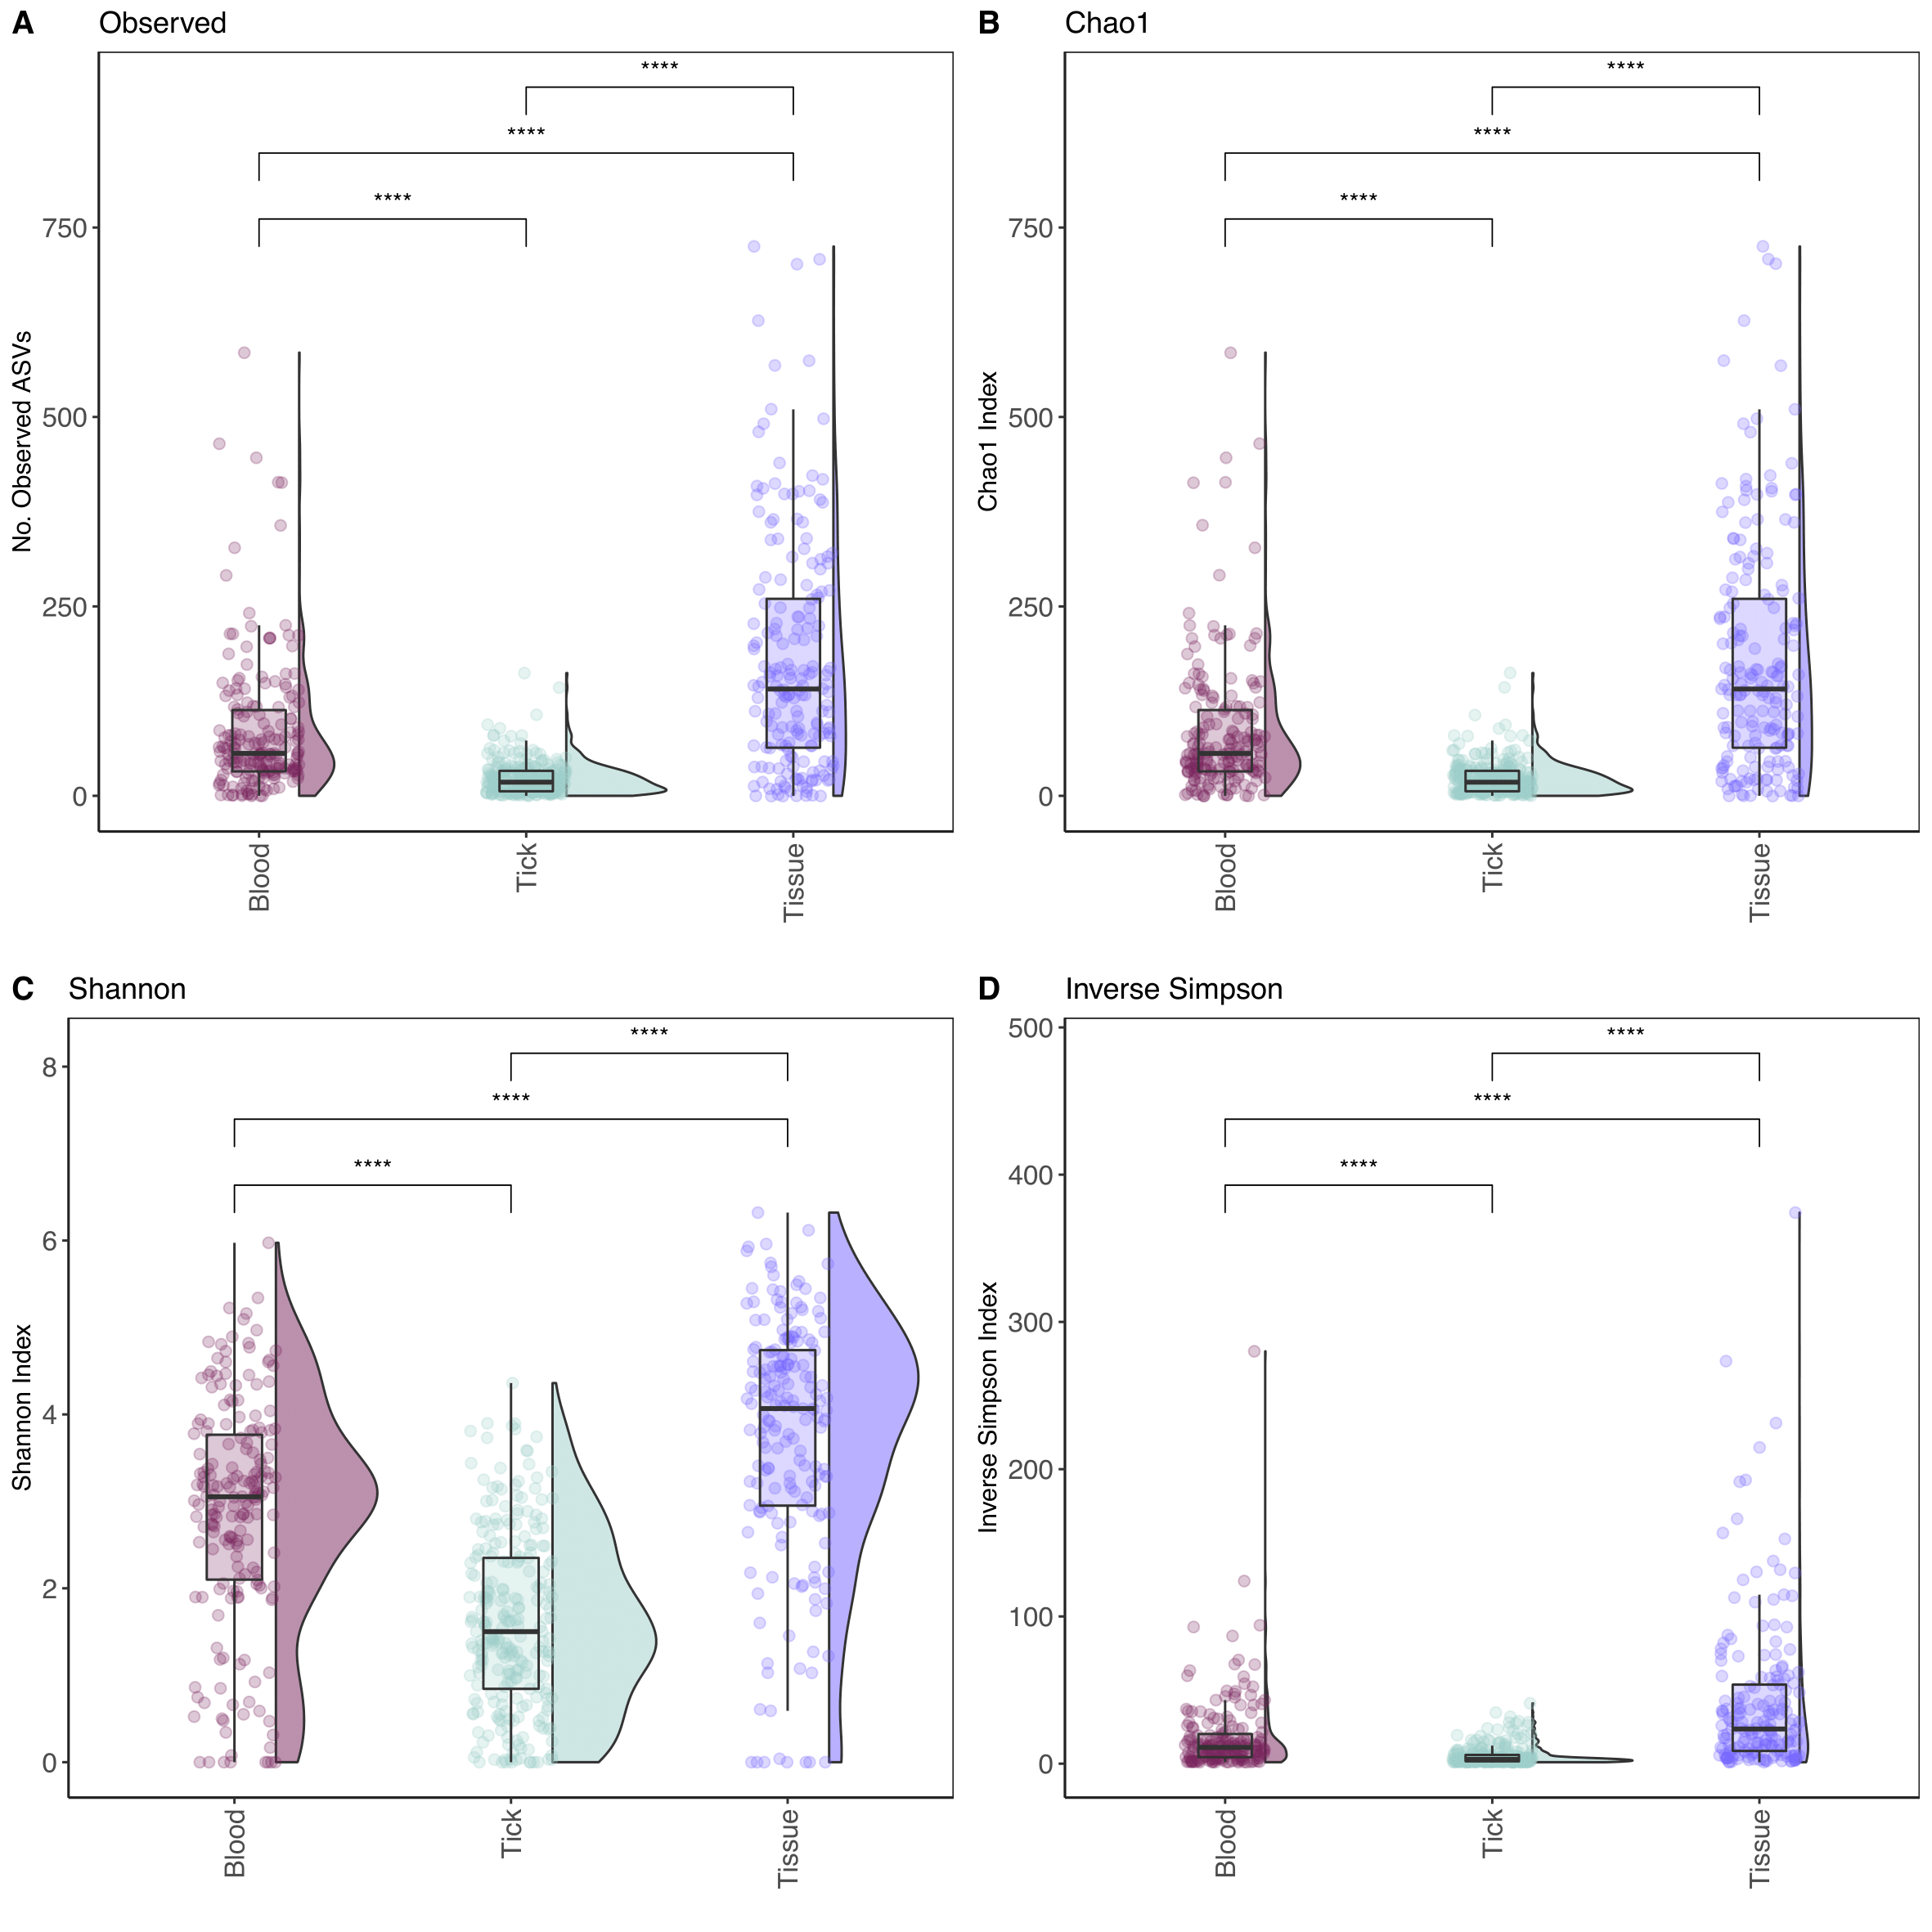
\includegraphics[width=0.95\linewidth]{figures/ms-figs/Ch3-alphadiv} \caption[Alpha diversity of microbiome community for wildlife blood, tissue and ticks.]{Boxplot of Alpha-diversity indices. Diversity indexes (A) Observed number of ASVs, (B) Chao1 index, (C) Shannon index and (D) inverse Simpson index. Boxplots and violin plots represent the distribution of diversity among samples within their category - blood (159), tick (205 pools) and tissue (172). Statistical analysis between sample types calculated using Wilcoxon pairwise (non-parametric) test with significance values indicated as follows: NS for P > 0.05; * for P <= 0.05; ** for P <= 0.01; *** for P <= 0.001; **** for P <= 0.0001.}\label{fig:F3alpha}
\end{figure}

In blood samples, the most abundant families were \emph{Bacillaceae} (22.9\%), \emph{Bartonellaceae} (11.3\%), \emph{Anaplasmataceae} (7.3\%) and \emph{Mycobacteriaceae} (2.6\%) (Figure \ref{fig:FA36}).
In tick samples the most abundant families were \emph{Coxiellaceae} (33.8\%), \emph{Midichloriaceae} (31.0\%), \emph{Mycobacteriaceae} (6.0\%), \emph{Flavobacteriaceae} (2.6\%) and \emph{Anaplasmataceae} (1.8\%) (Figure \ref{fig:FA37}).
In tissue samples the most abundant families were \emph{Staphylococcaceae} (8.2\%), \emph{Mycobacteriaceae} (6.5\%), \emph{Ruminococcaceae} (5.5\%), \emph{Flavobacteriaceae} (4.7\%) and \emph{Anaplasmataceae} (2.7\%) (Figure \ref{fig:FA38}).
Comparison of family taxa showed differences in abundance among sample types and species (and tick instar) (Figures \ref{fig:F3heatmap} and \ref{fig:F3heatmaptick}).

\begin{figure}
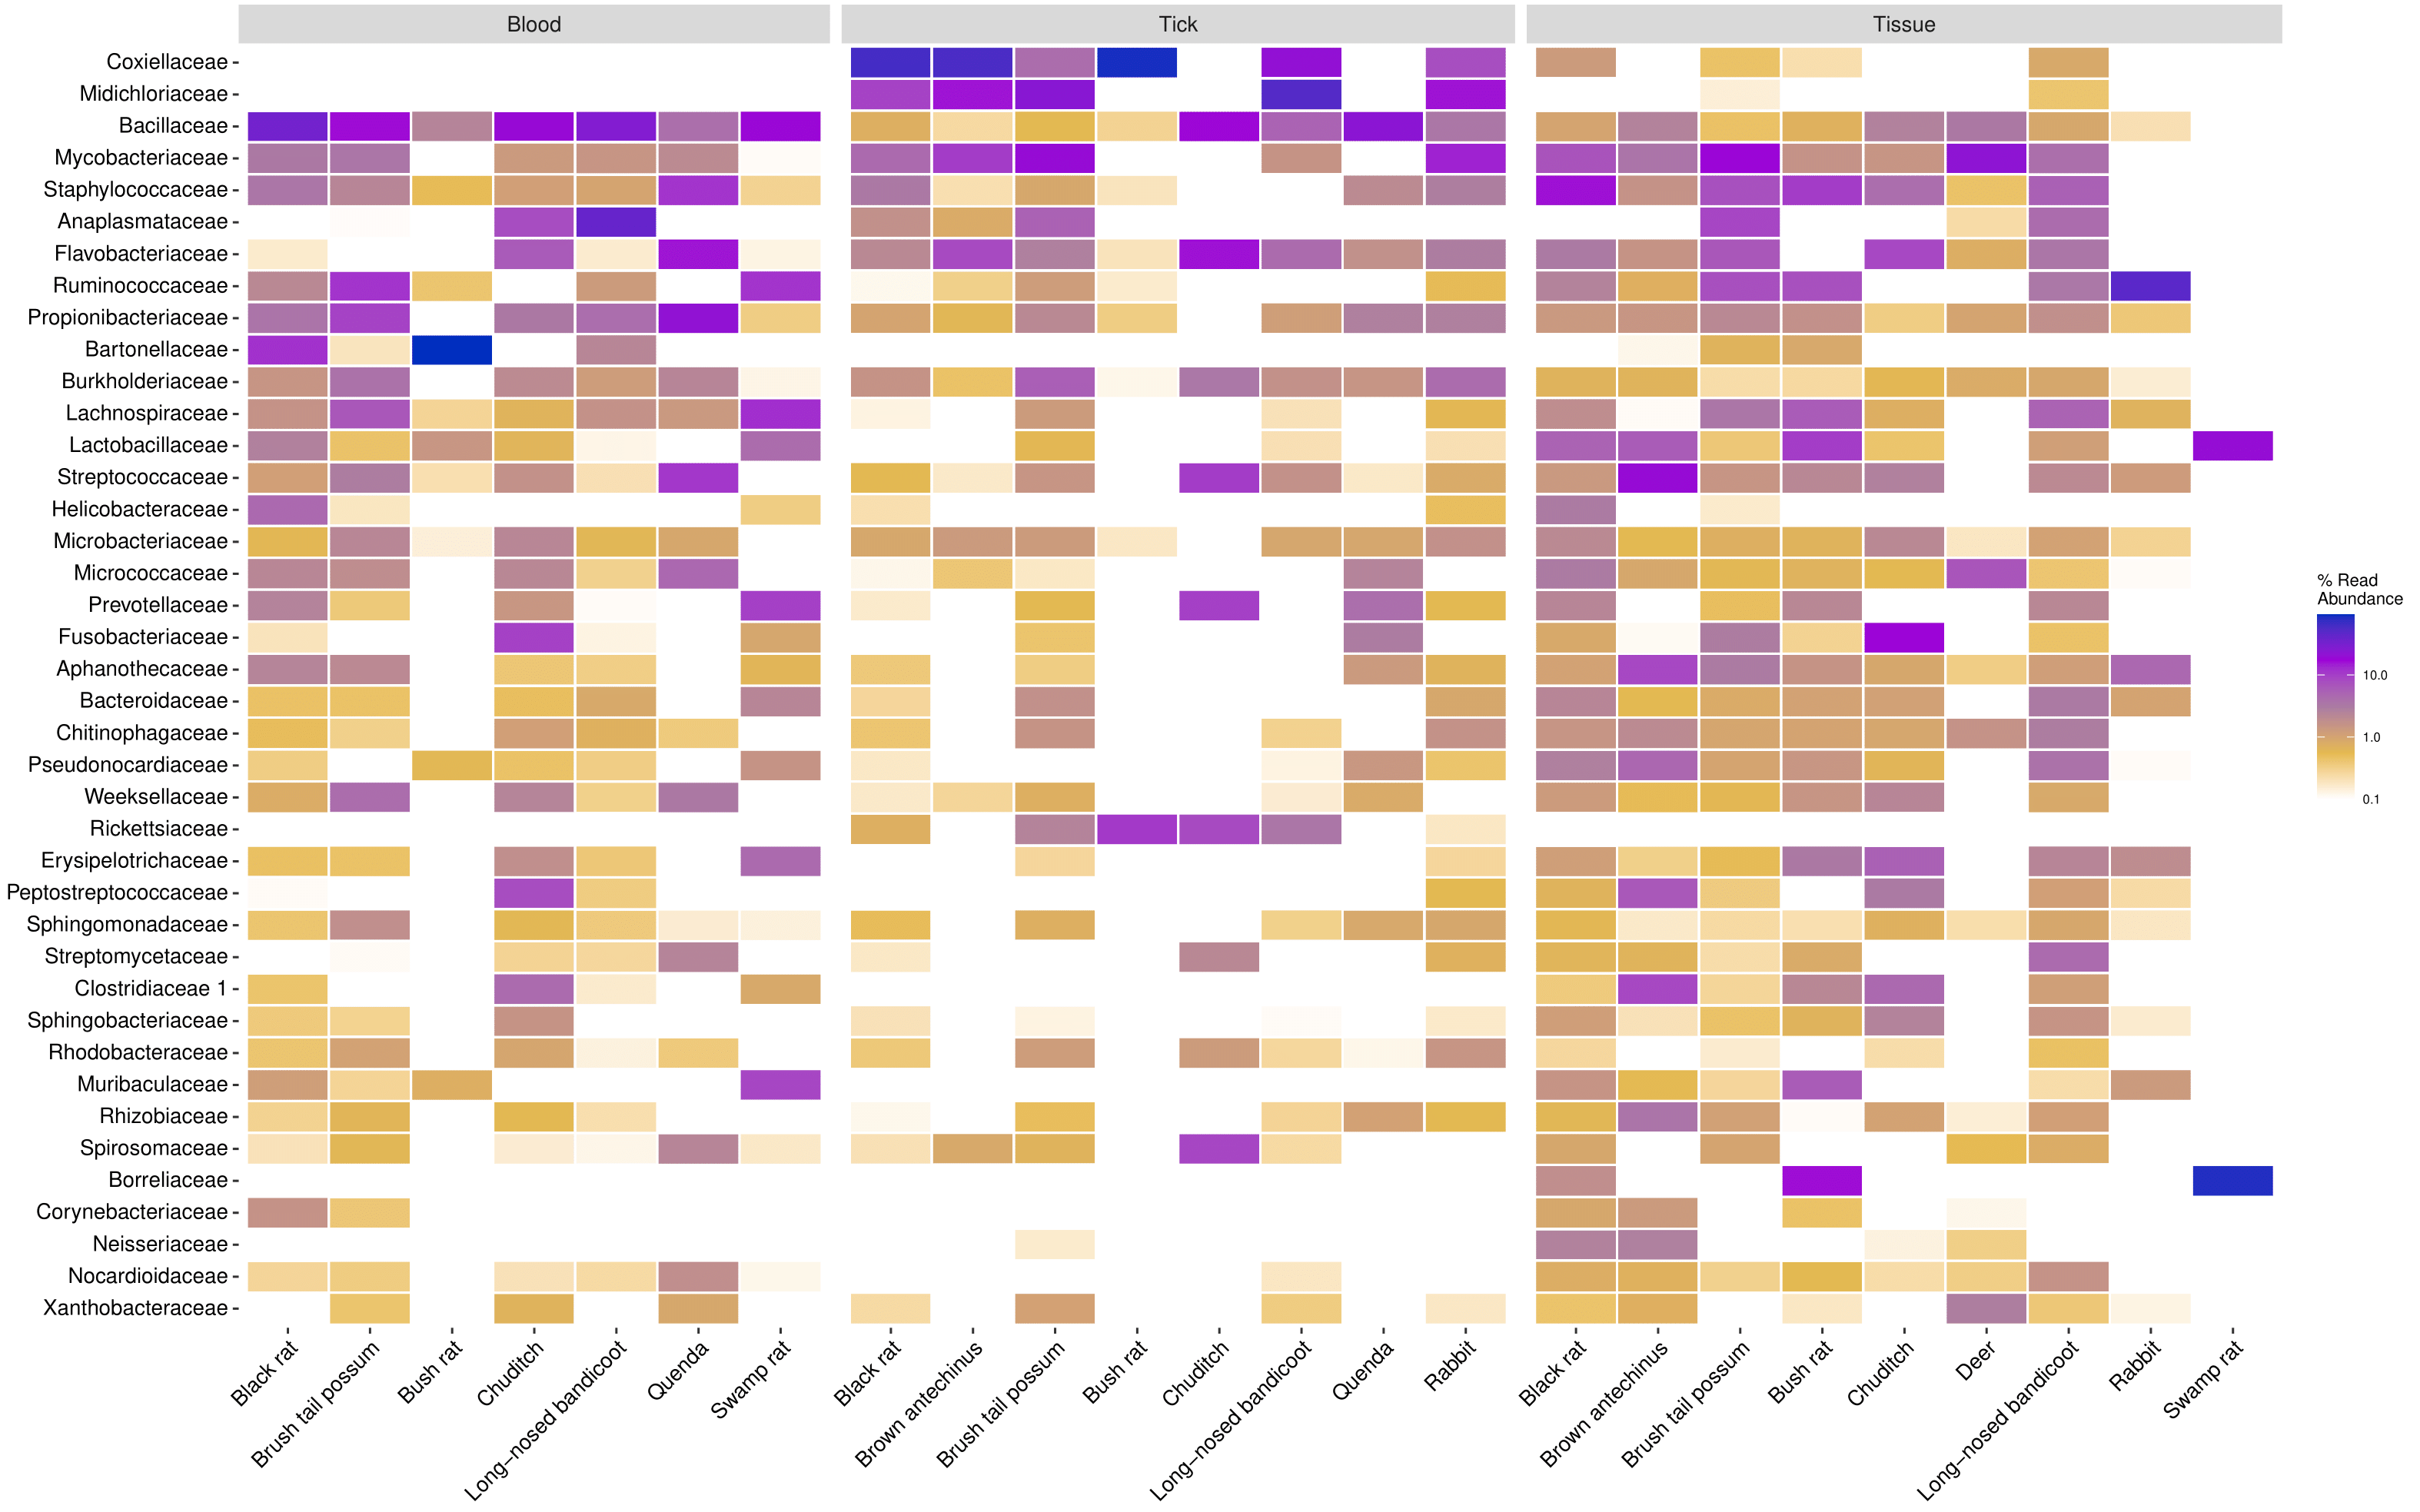
\includegraphics[width=0.95\linewidth]{figures/ms-figs/Ch3-heatmap} \caption[Heatmap of bacterial family taxa in wildlife samples.]{Heatmap of the top 40 most prevalent bacterial family taxa identified in wildlife blood, tick and tissue samples. Data first transformed to relative sequence abundance.}\label{fig:F3heatmap}
\end{figure}

\begin{figure}
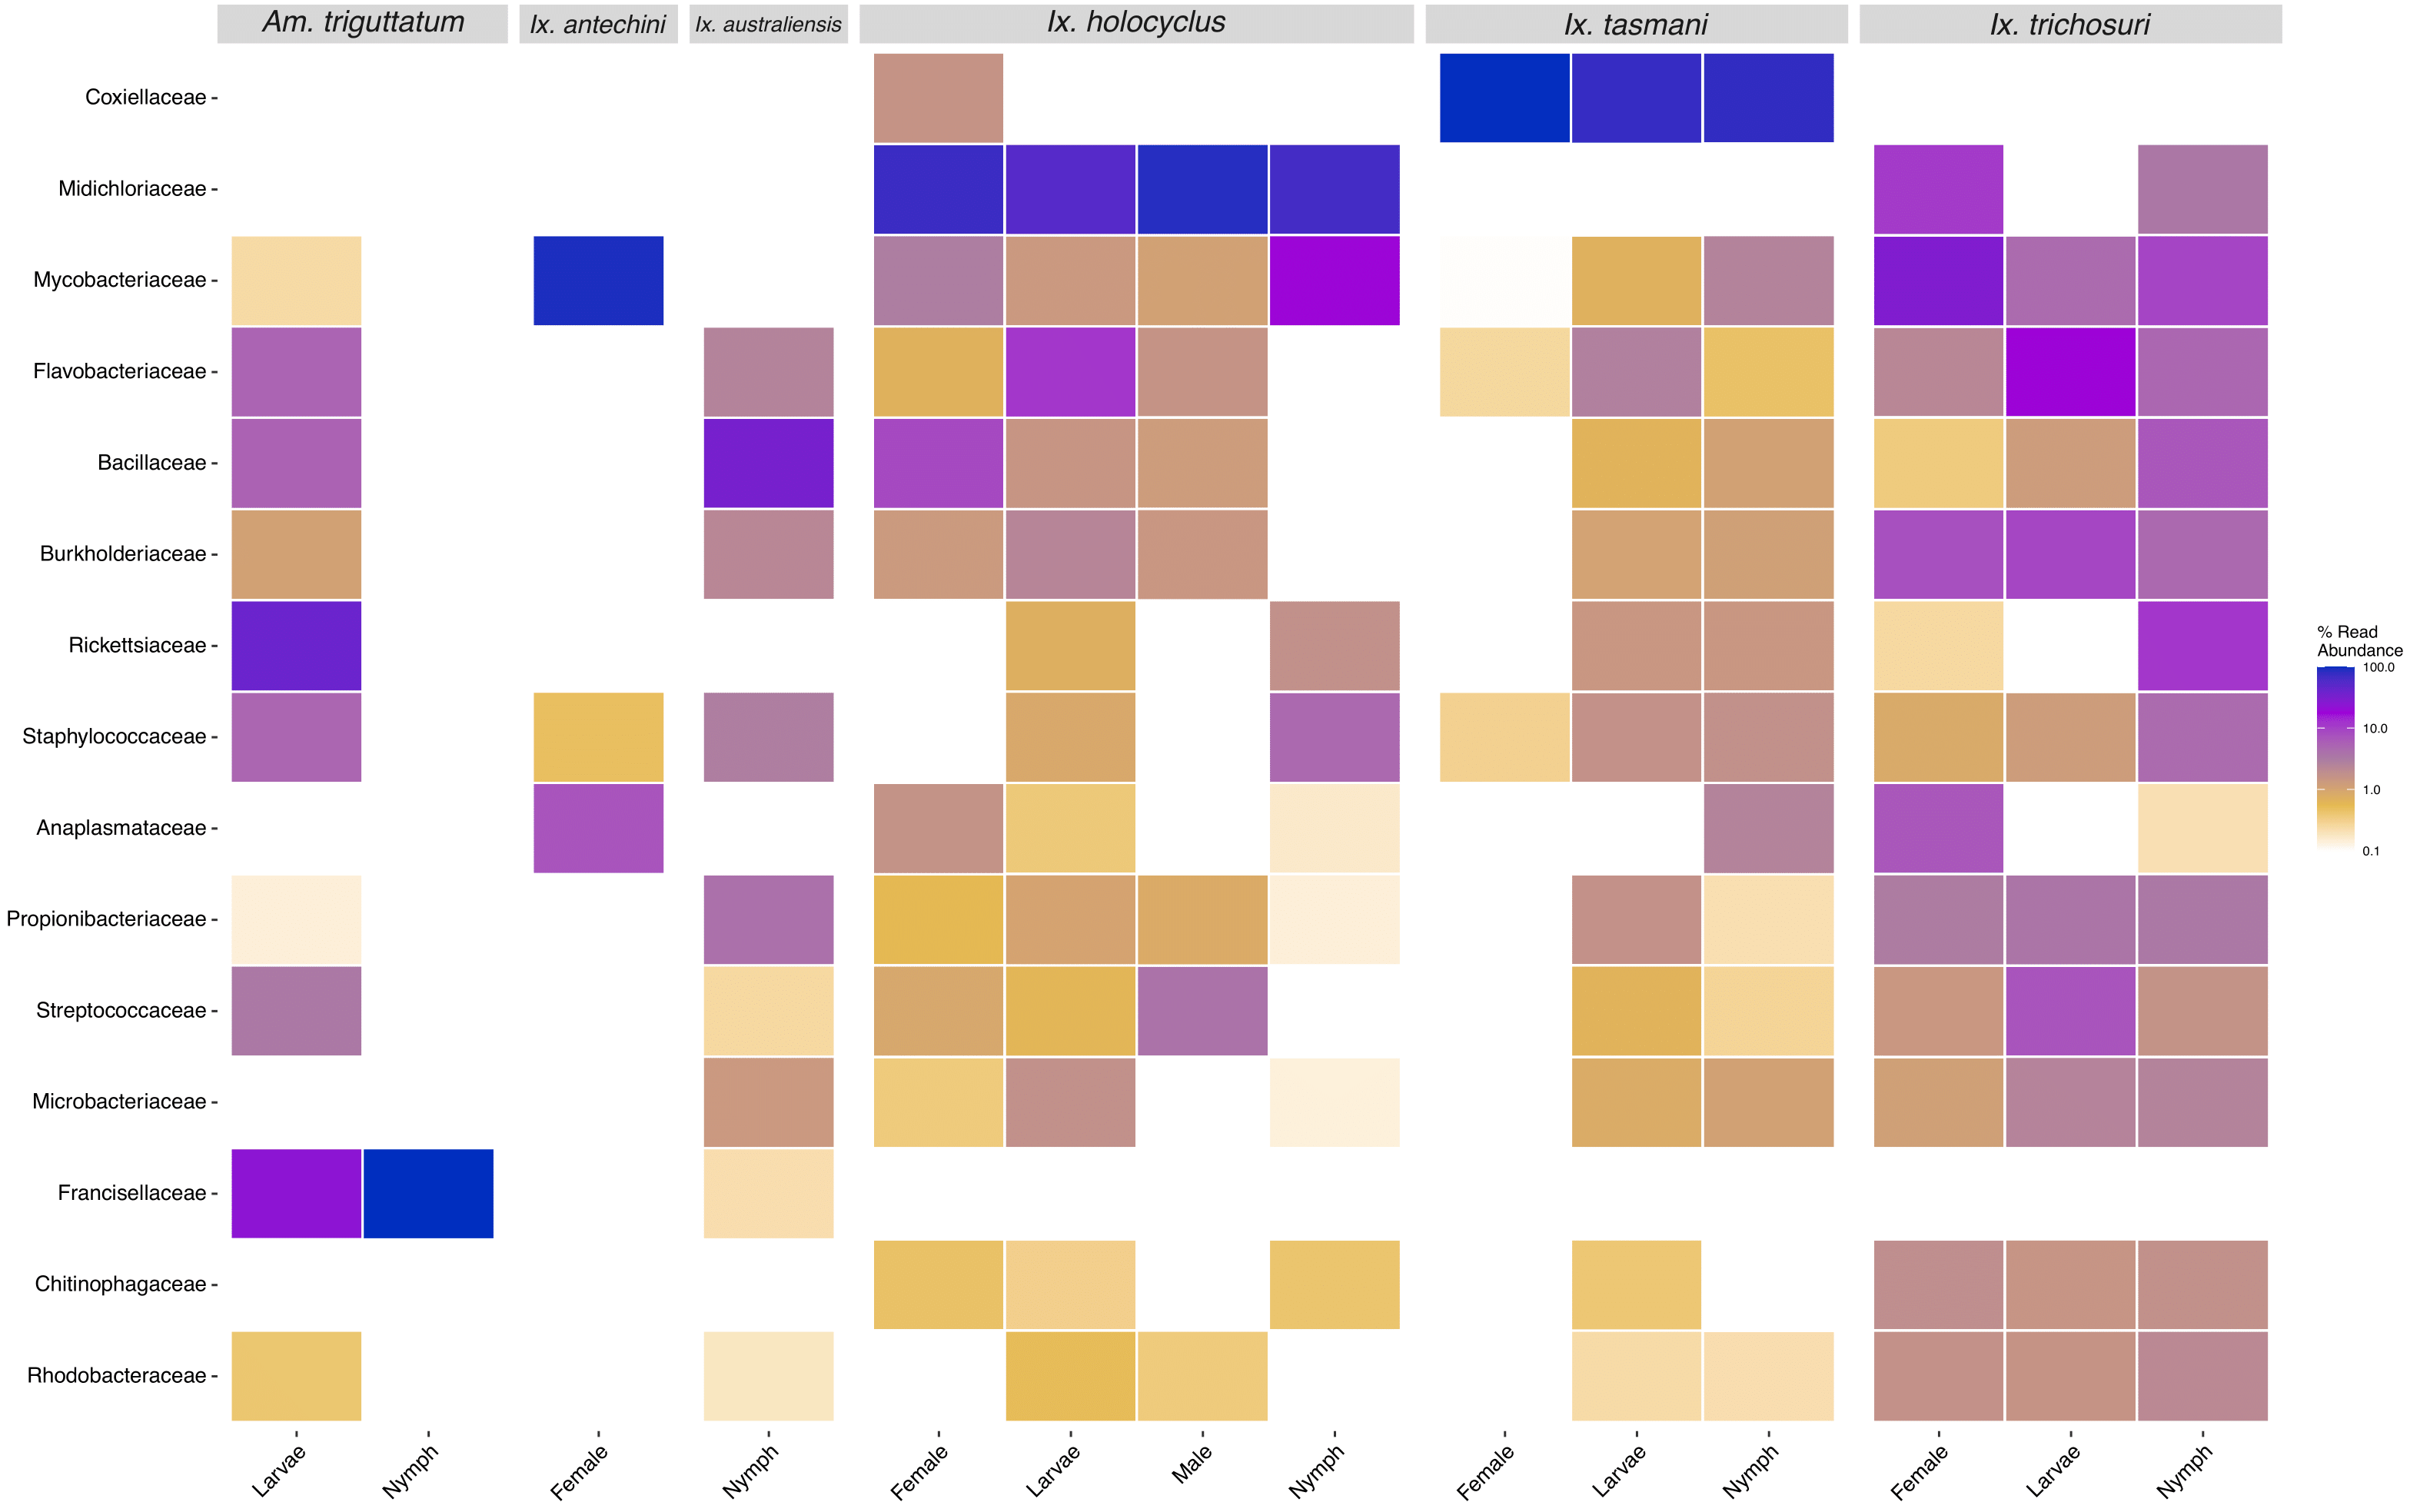
\includegraphics[width=0.95\linewidth]{figures/ms-figs/Ch3-heatmap-tick} \caption[Heatmap of bacterial family taxa in tick samples from wildlife.]{Heatmap of the top 15 most prevalent bacterial family taxa identified in tick samples, showing abundance in species and instar. Data first transformed to relative sequence abundance. Tick samples consisting of mixed species pools were excluded.}\label{fig:F3heatmaptick}
\end{figure}

The overlap of samples at the ASV level was investigated using various thresholds to define the `core microbiome', with two out of three models showing only seven shared ASVs between all three sample types (Figure \ref{fig:F3venn}).
Shared core microbiome ASVs of blood and tissue samples were compared between the four most abundant hosts samples and tick species (Figure \ref{fig:F3venn}).

\begin{figure}
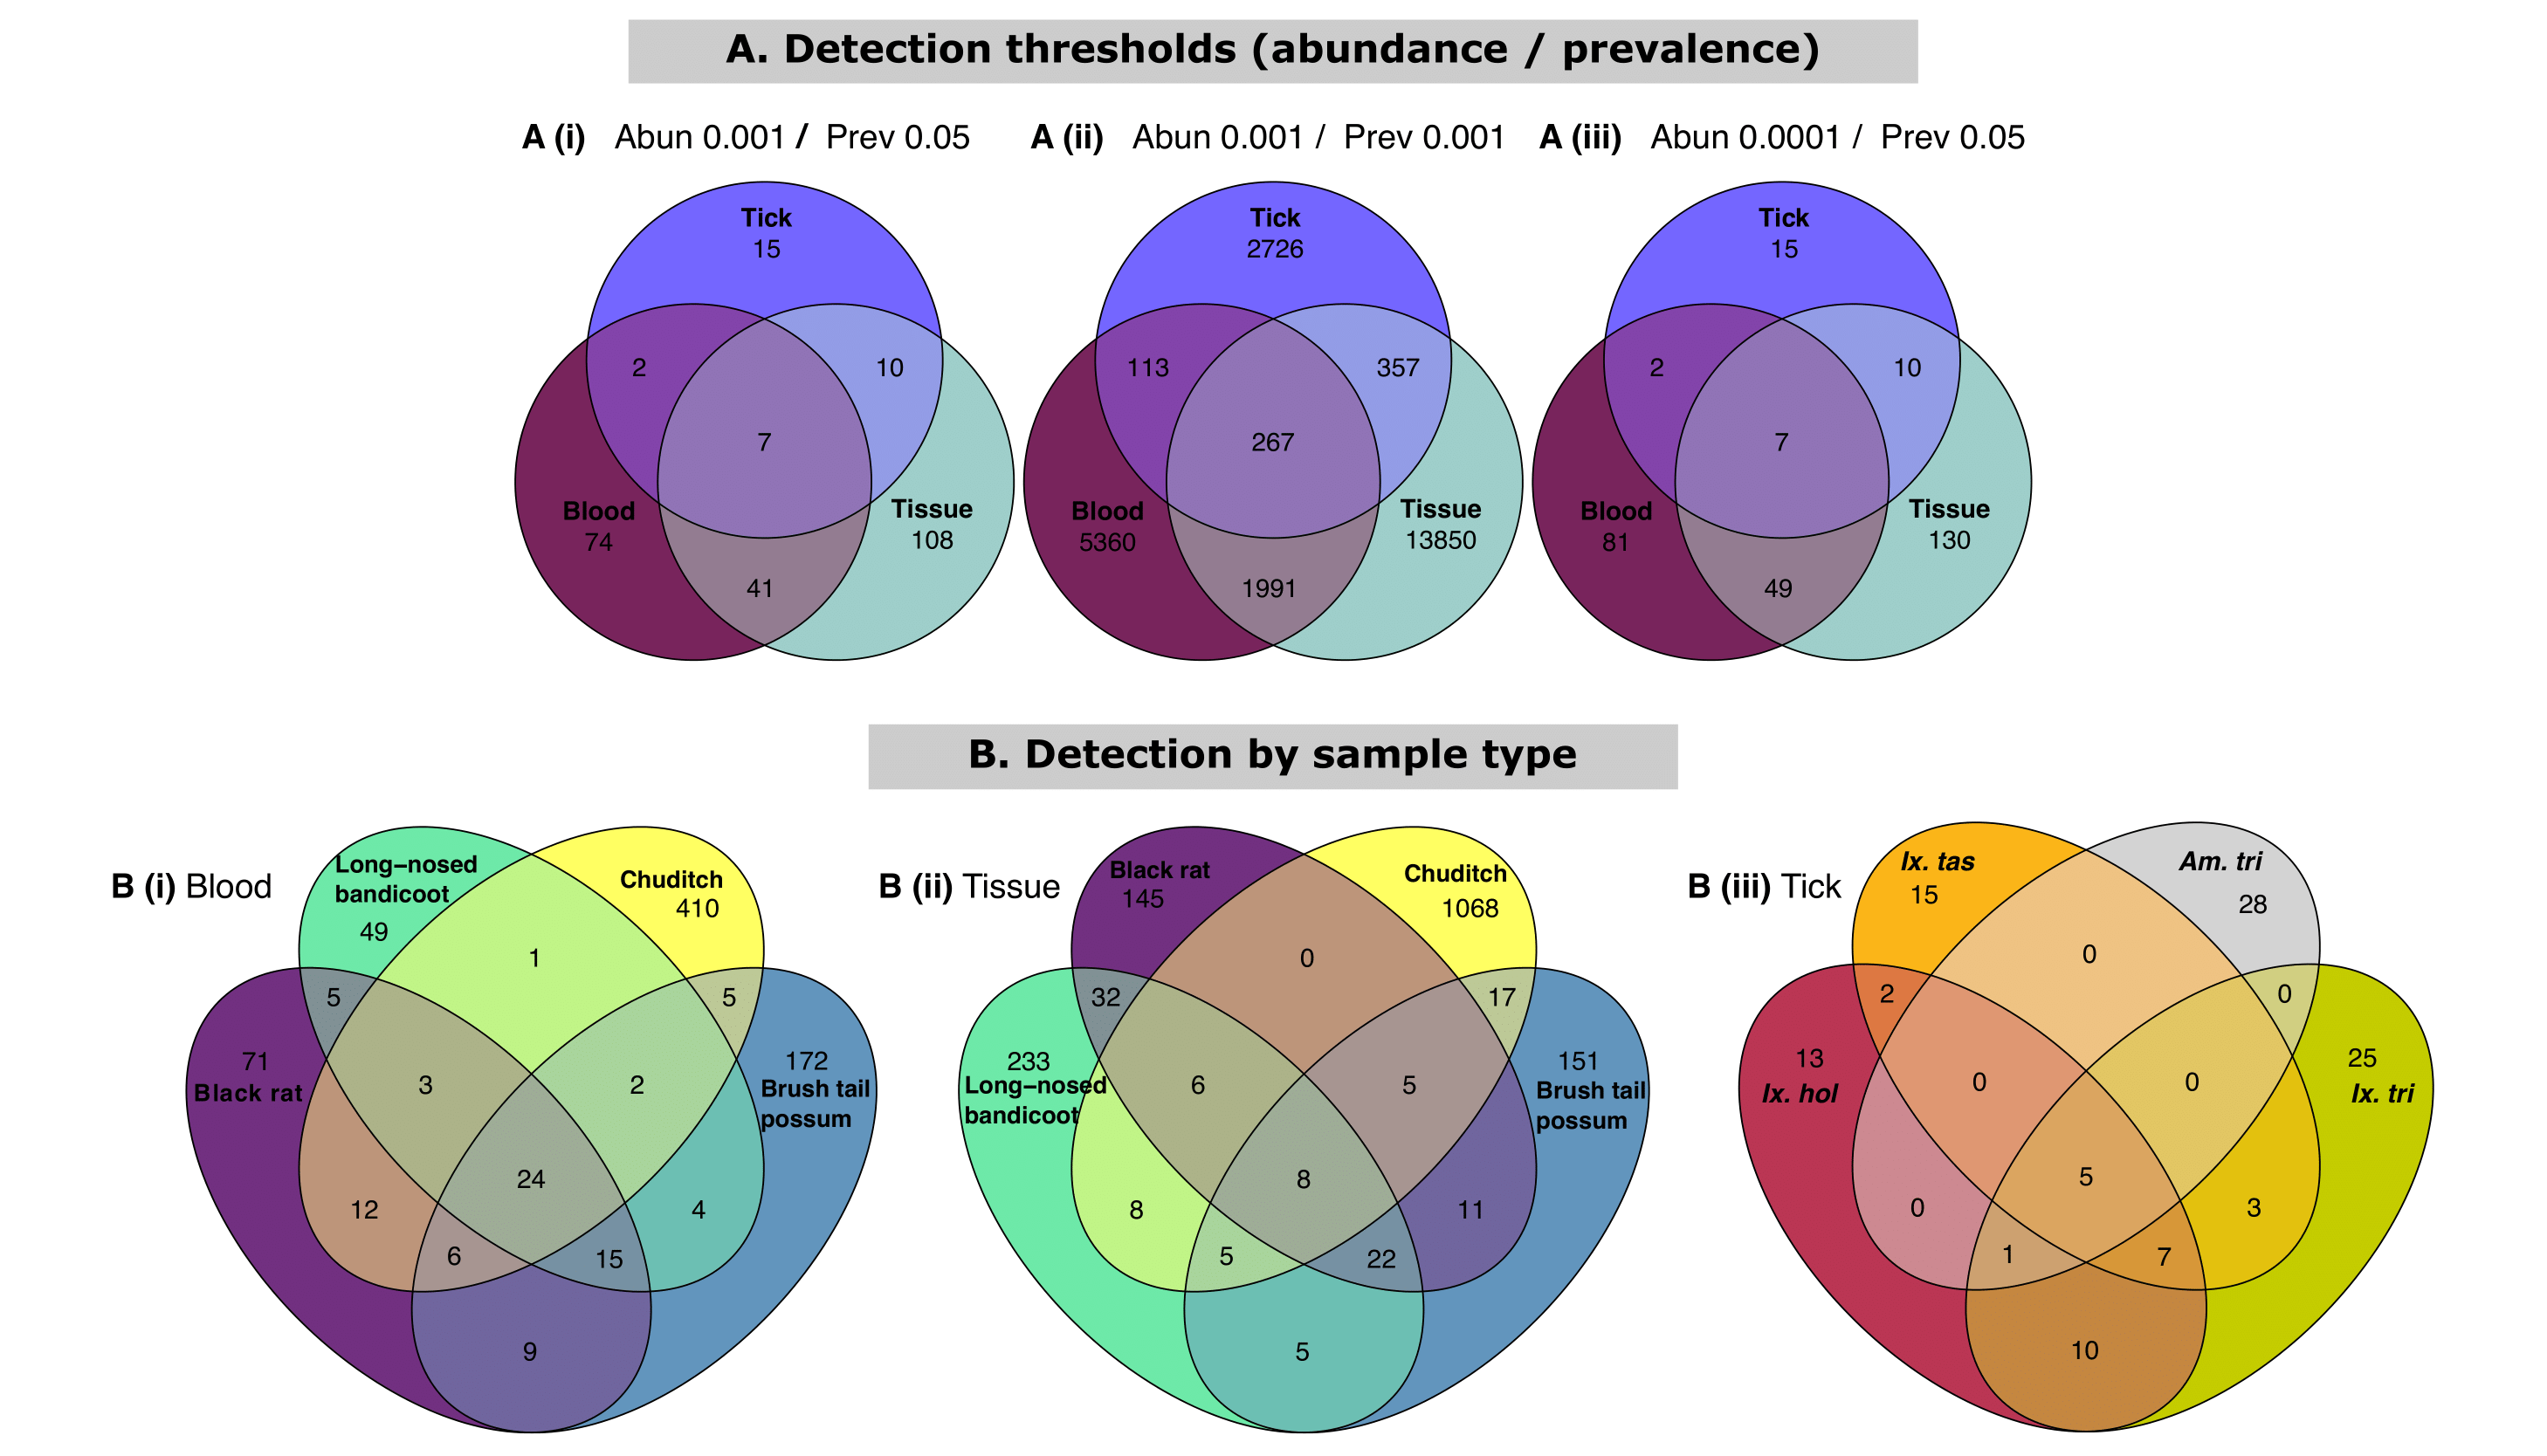
\includegraphics[width=0.95\linewidth]{figures/ms-figs/Ch3-venn_combine} \caption[Venn diagram of taxa present in blood, tick and tissues.]{Venn diagram of core taxa present within samples presented as detection of amplicon sequence variants (ASVs) using abundance and prevalence. Data first transformed to relative abundance and ASVs assigned to best hit. (A) Impact of similarity based on detection thresholds of abundance and prevalence as (i) 0.001 and 0.05, (ii) 0.001 and 0.001, (iii) 0.0001 and 0.05. (B) Core taxa present within sample types using detection levels set at 0.001 and 0.05 for abundance and prevalence respectively for (i) blood (ii) tissue and (iii) ticks. For within sample comparison only the four most abundant vertebrate host/tick species were selected. Tick species abbreviations: \textit{Amblyomma triguttatum} (\textit{Am. tri}), \textit{Ixodes holocyclus} (\textit{Ix. hol}), \textit{Ixodes tasmani} (\textit{Ix. tas}), \textit{Ixodes trichosuri} (\textit{Ix. tri}). Tick samples consisting of mixed species pools were excluded.}\label{fig:F3venn}
\end{figure}

Ordination analysis revealed a distinct difference between the bacterial composition of blood, tick and tissue samples (Figure \ref{fig:F3ord}). Hierarchical cluster analysis (Figure \ref{fig:FA39}) and statistical analysis (PERMANOVA F = 36.209, P = 0.001, see Supplementary Material \ref{ch3stats}) also supported this finding showing that there was a statistical difference in sample types, and there was little overlap in the microbiome composition of blood and tick samples.
Tissue samples were identified as an intermediate sample type and showed some (albeit low) similarities to blood and tick samples. Ordination analysis of tick samples showed distinction between tick species (Figure \ref{fig:F3ord}).
Tick species \emph{Ix. holocyclus} and \emph{Ix. trichosuri} showed the most similar bacterial composition with ordination analysis demonstrating overlap between these two species (PERMANOVA, F = 14.01, P = 0.001, see Supplementary Material \ref{ch3stats}).
Although sampling numbers were uneven among host species, which limited statistical inference, hierarchical cluster analysis did show that samples grouped were based on host (and tick) species (Figure \ref{fig:FA310}).

\begin{figure}
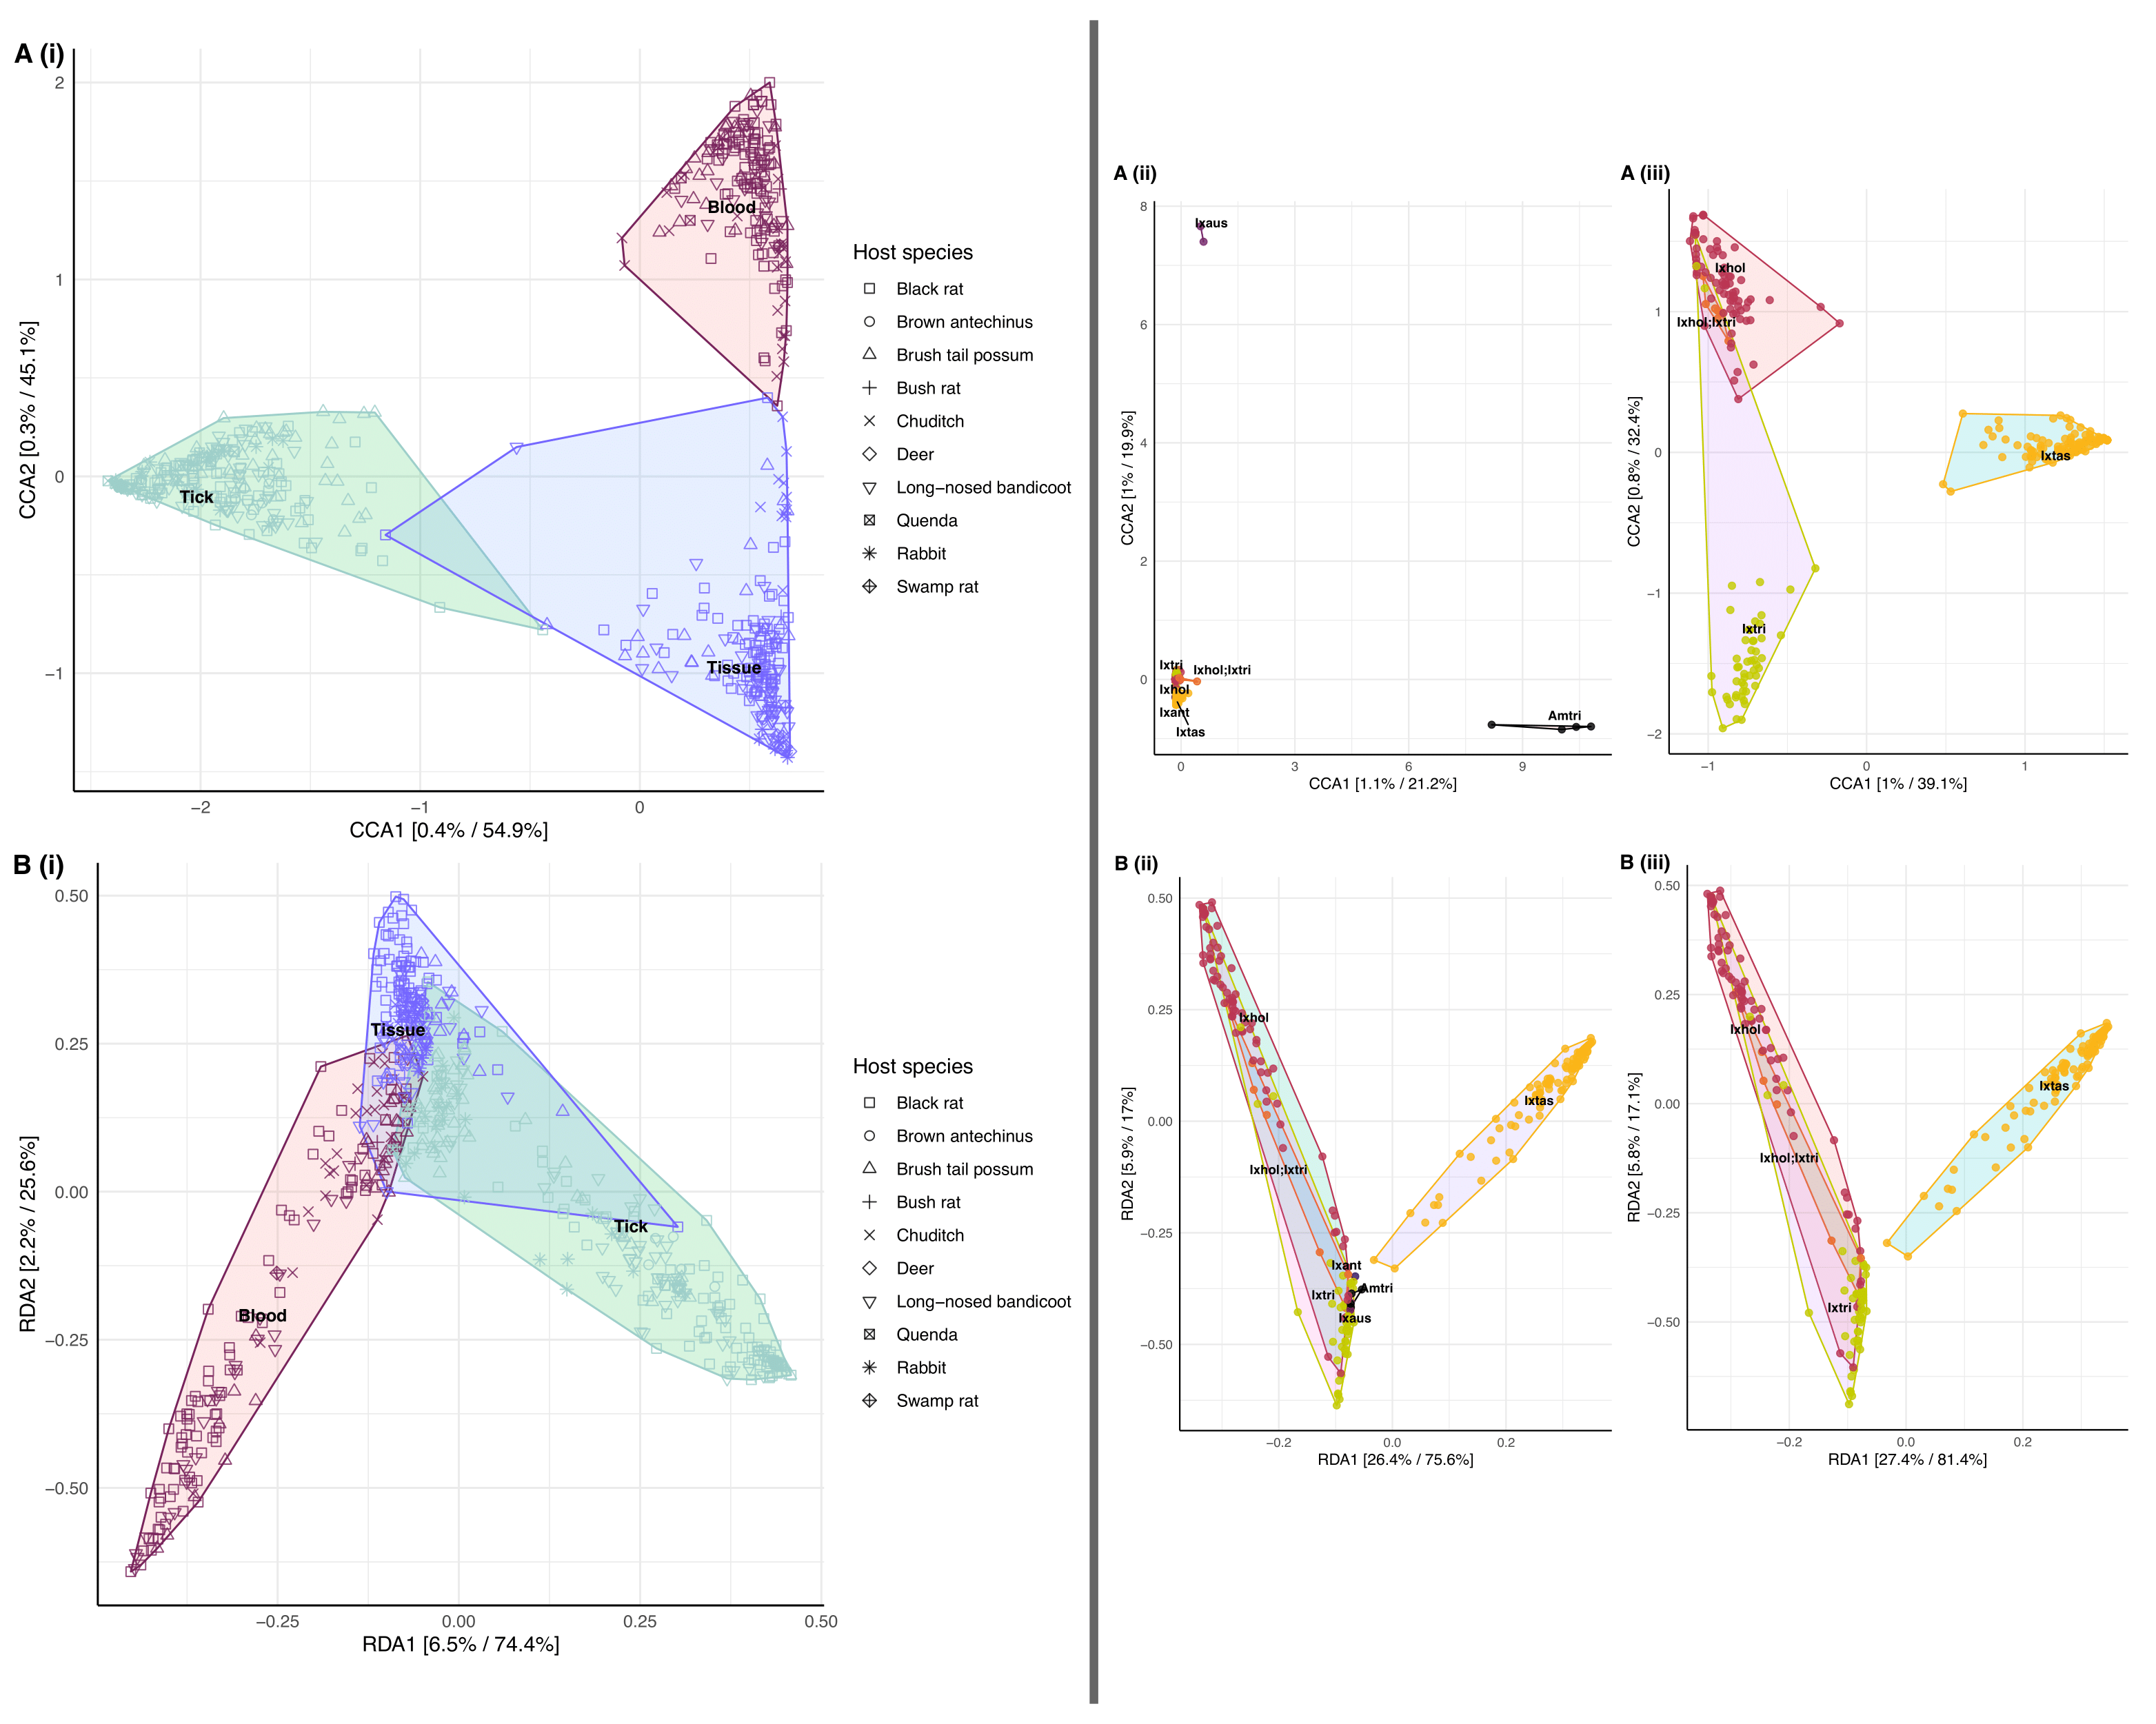
\includegraphics[width=0.95\linewidth]{figures/ms-figs/Ch3-ord_combine} \caption[Constrained ordination plot of microbiome composition from wildlife blood, tissue and ticks.]{Constrained ordination plot of microbiome composition from using constrained methods (A) Canonical Correspondence Analysis and (B) Redundancy Analysis (constrained Principal Component Analysis). (i) Ordination analysis of all samples N = 536 (159 blood, 205 tick pools, and 172 tissue) by sample type. (ii) Ordination of all tick samples by tick species (iii) Ordination of three co-habiting tick species in Sydney Northern Beaches area. Prior to the analysis ASVs < 0.1 relative abundance were removed. Analysis using the Hellinger transformation and Bray-Curtis distance measure. The relative contribution (eigen value) of each axis to the total inertia in the data as well as to the constrained space only, respectively, are indicated in percent at the axis titles. Tick species abbreviations: \textit{Amblyomma triguttatum} (\textit{Am. tri}),\textit{Ixodes antechinus} (\textit{Ix. ant}), \textit{Ixodes australiensis} (\textit{Ix. aus}), \textit{Ixodes holocyclus} (\textit{Ix. hol}), \textit{Ixodes tasmani} (\textit{Ix. tas}), \textit{Ixodes trichosuri} (\textit{Ix. tri}).}\label{fig:F3ord}
\end{figure}

\hypertarget{taxa-of-interest}{%
\subsection{Taxa of interest}\label{taxa-of-interest}}

Nine family taxa were chosen for comparison among sample types (Figure \ref{fig:F3tois}). \emph{Anaplasmataceae} bacteria were most prevalent in blood samples (both by relative abundance and prevalence). Blood and tissue samples showed no statistical difference in relative abundance (Wilcoxon pairwise test, P = 0.26), with significantly lower abundance in tick samples (Wilcoxon pairwise test, P \textless{} 0.001).
There was weak support for differences in \emph{Mycoplasmataceae} between sample types (Wilcoxon pairwise test, P = 0.023--0.43).
\emph{Midichloriaceae}, \emph{Coxielleaceae}, and \emph{Rickettsiaceae} were all significantly more abundant in ticks than blood or tissue samples.
Statistical comparisons of \emph{Borreliaceae} and \emph{Francisellaceae} were not made due to the small number of positive samples.

For subsequent prevalence analysis only taxa of interest that could be accurately defined to the genus level were retained (as per BLAST results). This identified 235 ASVs from 364 samples and 159 individuals see Table \ref{tab:T3prev} and full sequence data and BLAST results in \protect\hyperlink{supplementary-table-e1.1}{Supplementary Table E1.1}.

\begin{figure}
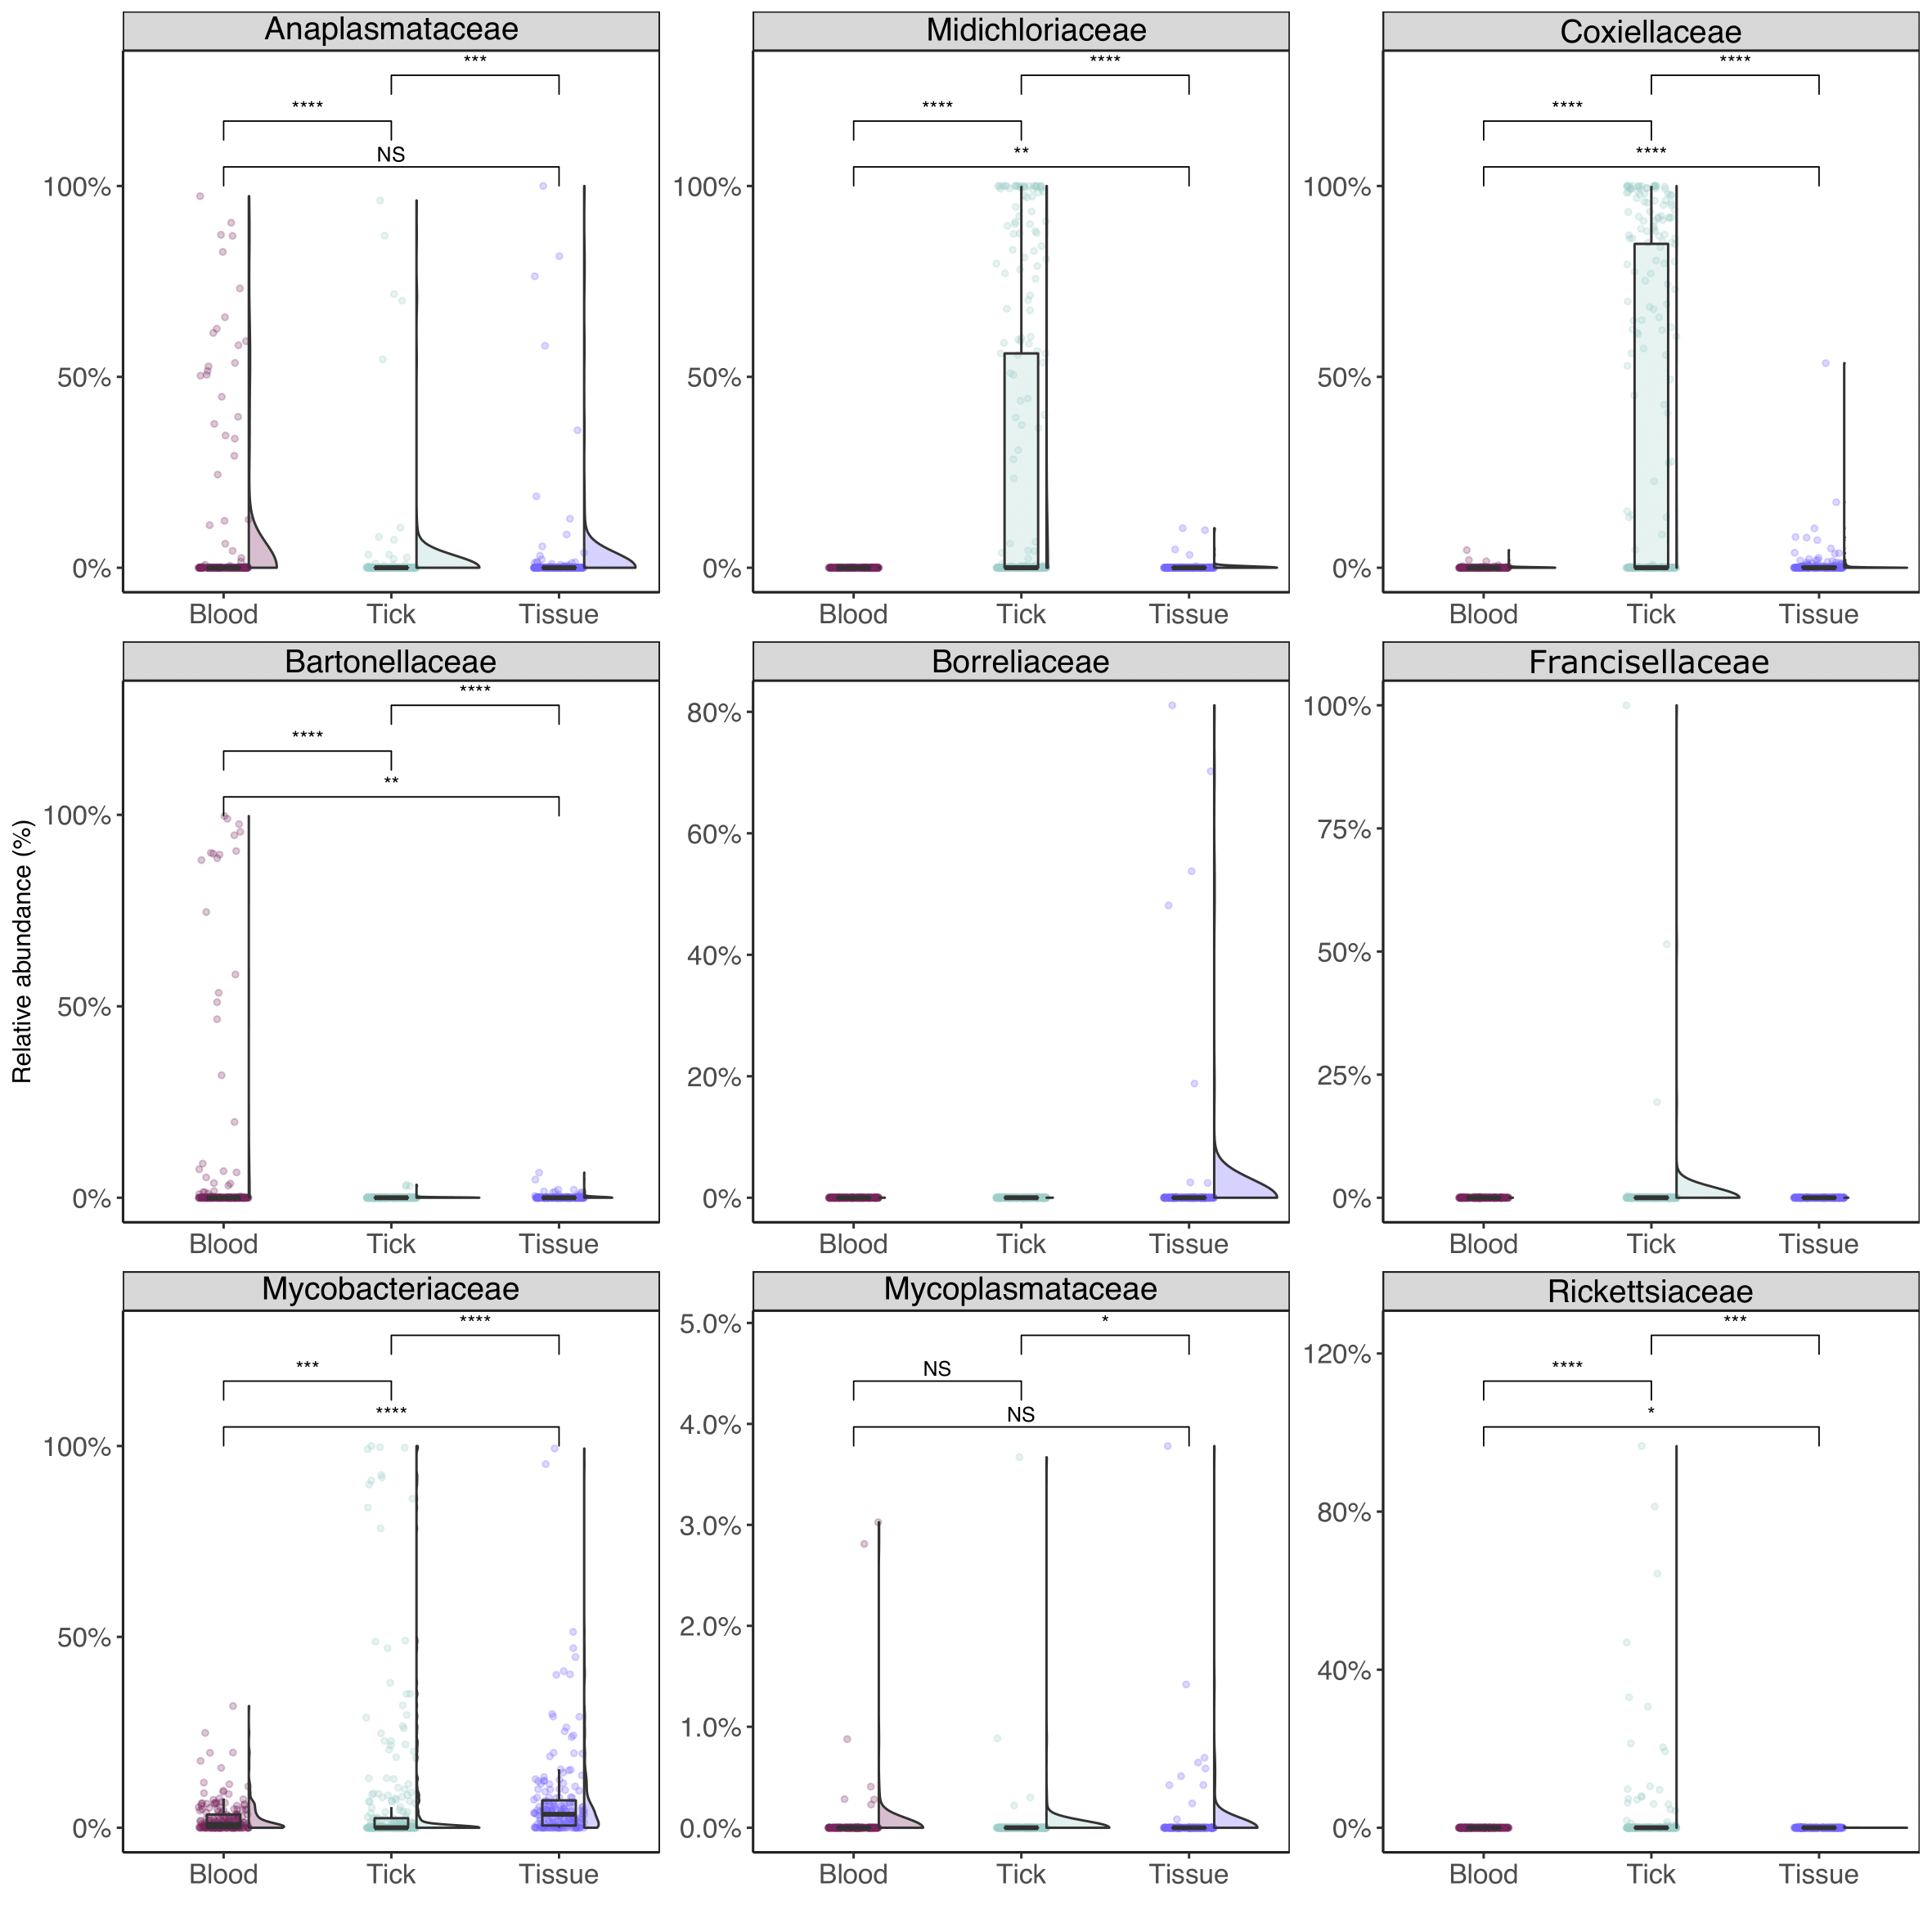
\includegraphics[width=0.95\linewidth]{figures/ms-figs/Ch3-toiboxplot} \caption[Relative abundance for select bacteria taxa from wildlife samples.]{Relative abundance for select bacteria taxa of interest (aggregated to family level) from wildlife samples. Statistical analysis between sample types calculated using Wilcoxon pairwise (non-parametric) test with significance values indicated as follows: NS for P > 0.05; * for P <= 0.05; ** for P <= 0.01; *** for P <= 0.001; **** for P <= 0.0001.}\label{fig:F3tois}
\end{figure}

\begin{landscape}\begin{table}

\caption[Bacteria 'taxa of interest' prevalence in wildlife and ticks.]{\label{tab:T3prev}Presence of 'taxa of interest'(a) by bacteria metabarcoding. Prevalence reported as proportion of individual hosts positive and proportion of samples positive in parenthesis (accounting for instances where more than one sample type was collected from an individual).}
\centering
\fontsize{8.5}{10.5}\selectfont
\begin{tabular}[t]{>{}l>{}lllllllllll}
\toprule
Taxa of interest & Sample type & Black rat & Brown antechinus & Brush tail possum & Bush rat & Chuditch & Deer & Long-nosed bandicoot & Quenda & Rabbit & Swamp rat\\
\midrule
\em{Anaplasmataceae} & \textbf{Blood} & 4/68 (4/84) & 0/0 (0/0) & 5/18 (6/21) & 0/2 (0/2) & 7/22 (9/24) & 0/0 (0/0) & 18/20 (22/25) & 0/1 (0/2) & 0/0 (0/0) & 0/1 (0/1)\\
\em{} & \textbf{Tick} & 3/54 (3/79) & 1/4 (1/6) & 4/15 (5/33) & 0/3 (0/4) & 0/1 (0/1) & 0/0 (0/0) & 8/31 (9/60) & 0/2 (0/2) & 0/7 (0/20) & 0/0 (0/0)\\
\em{} & \textbf{Tissue} & 6/71 (8/80) & 0/2 (0/2) & 4/16 (5/20) & 0/3 (0/3) & 1/9 (1/9) & 3/3 (3/6) & 18/40 (19/44) & 0/0 (0/0) & 0/7 (0/7) & 0/1 (0/1)\\
\em{Bartonella} & \textbf{Blood} & 22/68 (27/84) & 0/0 (0/0) & 7/18 (8/21) & 2/2 (2/2) & 0/22 (0/24) & 0/0 (0/0) & 4/20 (4/25) & 0/1 (0/2) & 0/0 (0/0) & 0/1 (0/1)\\
\em{} & \textbf{Tick} & 3/54 (4/79) & 0/4 (0/6) & 0/15 (0/33) & 1/3 (1/4) & 0/1 (0/1) & 0/0 (0/0) & 1/31 (1/60) & 0/2 (0/2) & 0/7 (0/20) & 0/0 (0/0)\\
\em{} & \textbf{Tissue} & 4/71 (5/80) & 1/2 (1/2) & 9/16 (11/20) & 2/3 (2/3) & 0/9 (0/9) & 0/3 (0/6) & 3/40 (3/44) & 0/0 (0/0) & 0/7 (0/7) & 0/1 (0/1)\\
\em{Borrelia} & \textbf{Blood} & 0/68 (0/84) & 0/0 (0/0) & 0/18 (0/21) & 0/2 (0/2) & 0/22 (0/24) & 0/0 (0/0) & 0/20 (0/25) & 0/1 (0/2) & 0/0 (0/0) & 0/1 (0/1)\\
\em{} & \textbf{Tick} & 0/54 (0/79) & 0/4 (0/6) & 0/15 (0/33) & 0/3 (0/4) & 0/1 (0/1) & 0/0 (0/0) & 0/31 (0/60) & 0/2 (0/2) & 0/7 (0/20) & 0/0 \vphantom{1} (0/0)\\
\em{} & \textbf{Tissue} & 7/71 (7/80) & 0/2 (0/2) & 0/16 (0/20) & 1/3 (1/3) & 0/9 (0/9) & 0/3 (0/6) & 0/40 (0/44) & 0/0 (0/0) & 0/7 (0/7) & 1/1 (1/1)\\
\em{Coxiellaceae} & \textbf{Blood} & 7/68 (7/84) & 0/0 (0/0) & 1/18 (1/21) & 0/2 (0/2) & 0/22 (0/24) & 0/0 (0/0) & 3/20 (5/25) & 0/1 (0/2) & 0/0 (0/0) & 0/1 (0/1)\\
\em{} & \textbf{Tick} & 50/54 (63/79) & 3/4 (4/6) & 8/15 (9/33) & 3/3 (4/4) & 0/1 (0/1) & 0/0 (0/0) & 22/31 (24/60) & 0/2 (0/2) & 2/7 (2/20) & 0/0 (0/0)\\
\em{} & \textbf{Tissue} & 33/71 (38/80) & 0/2 (0/2) & 2/16 (2/20) & 2/3 (2/3) & 0/9 (0/9) & 0/3 (0/6) & 20/40 (22/44) & 0/0 (0/0) & 0/7 (0/7) & 0/1 (0/1)\\
\em{Francisellaceae} & \textbf{Blood} & 0/68 (0/84) & 0/0 (0/0) & 0/18 (0/21) & 0/2 (0/2) & 0/22 (0/24) & 0/0 (0/0) & 0/20 (0/25) & 0/1 (0/2) & 0/0 (0/0) & 0/1 (0/1)\\
\em{} & \textbf{Tick} & 0/54 (0/79) & 0/4 (0/6) & 2/15 (2/33) & 0/3 (0/4) & 0/1 (0/1) & 0/0 (0/0) & 0/31 (0/60) & 2/2 (2/2) & 0/7 (0/20) & 0/0 (0/0)\\
\em{} & \textbf{Tissue} & 0/71 (0/80) & 0/2 (0/2) & 0/16 (0/20) & 0/3 (0/3) & 0/9 (0/9) & 0/3 (0/6) & 0/40 (0/44) & 0/0 (0/0) & 0/7 (0/7) & 0/1 \vphantom{1} (0/1)\\
\em{Midichloria} & \textbf{Blood} & 0/68 (0/84) & 0/0 (0/0) & 0/18 (0/21) & 0/2 (0/2) & 0/22 (0/24) & 0/0 (0/0) & 0/20 (0/25) & 0/1 (0/2) & 0/0 (0/0) & 0/1 (0/1)\\
\em{} & \textbf{Tick} & 17/54 (21/79) & 2/4 (2/6) & 12/15 (20/33) & 0/3 (0/4) & 0/1 (0/1) & 0/0 (0/0) & 19/31 (41/60) & 0/2 (0/2) & 5/7 (10/20) & 0/0 (0/0)\\
\em{} & \textbf{Tissue} & 5/71 (5/80) & 0/2 (0/2) & 1/16 (1/20) & 0/3 (0/3) & 0/9 (0/9) & 0/3 (0/6) & 3/40 (3/44) & 0/0 (0/0) & 0/7 (0/7) & 0/1 (0/1)\\
\em{Mycoplasma} & \textbf{Blood} & 1/68 (1/84) & 0/0 (0/0) & 0/18 (0/21) & 0/2 (0/2) & 0/22 (0/24) & 0/0 (0/0) & 0/20 (0/25) & 0/1 (0/2) & 0/0 (0/0) & 1/1 (1/1)\\
\em{} & \textbf{Tick} & 0/54 (0/79) & 0/4 (0/6) & 0/15 (0/33) & 0/3 (0/4) & 0/1 (0/1) & 0/0 (0/0) & 0/31 (0/60) & 0/2 (0/2) & 0/7 (0/20) & 0/0 (0/0)\\
\em{} & \textbf{Tissue} & 1/71 (1/80) & 0/2 (0/2) & 0/16 (0/20) & 0/3 (0/3) & 0/9 (0/9) & 0/3 (0/6) & 0/40 (0/44) & 0/0 (0/0) & 0/7 (0/7) & 0/1 (0/1)\\
\em{Rickettsia} & \textbf{Blood} & 0/68 (0/84) & 0/0 (0/0) & 0/18 (0/21) & 0/2 (0/2) & 0/22 (0/24) & 0/0 (0/0) & 0/20 (0/25) & 0/1 (0/2) & 0/0 (0/0) & 0/1 (0/1)\\
\em{} & \textbf{Tick} & 7/54 (7/79) & 0/4 (0/6) & 2/15 (2/33) & 2/3 (3/4) & 1/1 (1/1) & 0/0 (0/0) & 9/31 (10/60) & 0/2 (0/2) & 1/7 (1/20) & 0/0 (0/0)\\
\em{} & \textbf{Tissue} & 0/71 (0/80) & 0/2 (0/2) & 0/16 (0/20) & 0/3 (0/3) & 0/9 (0/9) & 0/3 (0/6) & 0/40 (0/44) & 0/0 (0/0) & 0/7 (0/7) & 0/1 (0/1)\\
\bottomrule
\multicolumn{12}{l}{\rule{0pt}{1em}\textsuperscript{a} Taxa of interest are defined as bacteria related to known pathogens associated with ticks and other vectors described globally, as outlined in Egan et al. 2020.}\\
\end{tabular}
\end{table}
\end{landscape}

\hypertarget{anaplasmataceae-2}{%
\subsubsection{\texorpdfstring{\emph{Anaplasmataceae}}{Anaplasmataceae}}\label{anaplasmataceae-2}}

The \emph{Anaplasmataceae} family was identified in 95 samples from 59 individuals.
The most prevalent genera were \emph{Neoehrlichia} (43 individuals), followed by \emph{Ehrlichia} (eight individuals) than \emph{Anaplasma} (three individuals).

`\emph{Candidatus} Neoehrlichia arcana' was identified in 52 samples: 29 blood, seven ticks (\emph{Ix. holocyclus}), and 16 tissue. `\emph{Candidatus} Neoehrlichia australis' was identified in 33 samples: eight blood, six ticks (\emph{Ix. holocyclus}, \emph{Ix. trichosuri}), and 19 tissue.
Sixteen samples had mixed infections of `\emph{Ca}. N. arcana' and `\emph{Ca}. N. australis' (six blood and ten tissue).
No ticks had mixed \emph{Neoehrlichia} infections.
Three putative novel \emph{Anaplasmataceae} species were identified from the present study, two \emph{Ehrlichia} spp. and a single \emph{Neoehrlichia} sp.
The novel \emph{Neoehrlichia} sp. was identified in three samples: a tissue sample from a black rat and a corresponding tick from the same individual (\emph{Ix. tasmani}); and a tick from a brown antechinus (\emph{Ix. antechini}).
One novel \emph{Ehrlichia} sp. was identified in five samples from two brush-tailed possums: two blood, one tick (\emph{Ix. holocyclus}) and two tissue.
A second novel \emph{Ehrlichia} sp. was identified in seven samples from six chuditch (six blood and one tissue). Only one chuditch was positive in corresponding tissue and blood samples.
Three deer tissue samples were infected with \emph{Anaplasma platys} (\protect\hyperlink{supplementary-table-e1.1}{Supplementary Table E1.1}).
Detection of \emph{Anaplasmataceae} bacteria differed between tick species and instars.
\emph{Ixodes holocyclus} females had the highest prevalence of this taxon, followed by nymph and larval ticks, while no males were positive (Figure \ref{fig:F3heatmaptick}).
Only \emph{Ix. tasmani} nymph samples were positive and in the case of \emph{Ix. trichosuri}, females and nymphs were identified with \emph{Anaplasmataceae} and all larvae were negative.

Phylogenetic analysis was performed using a 1,244 bp fragment of the 16S rRNA locus (Figure \ref{fig:F3anaplas}).
All `\emph{Ca}. N. arcana' amplified were identical to each other and showed 100\% similarity to `\emph{Ca}. Neoehrlichia arcana' isolate HT94 from \emph{Ix. holocyclus}, Australia (KU865447).
\emph{Ehrlichia} sequences from chuditch blood samples were 100\% identical to each other and most similar to \emph{Ehrlichia} sp. Anan from \emph{Ix. ovatus}, Japan (AB028319, 98.94\% similarity).
The nearest named species was \emph{Ehrlichia muris} (CP006917, 98.86\% similarity) isolated from a wild mouse (\emph{Eothenomys kageus}) in Japan (genetic distances \protect\hyperlink{supplementary-table-e1.2}{Supplementary Table E1.2}).

\begin{figure}
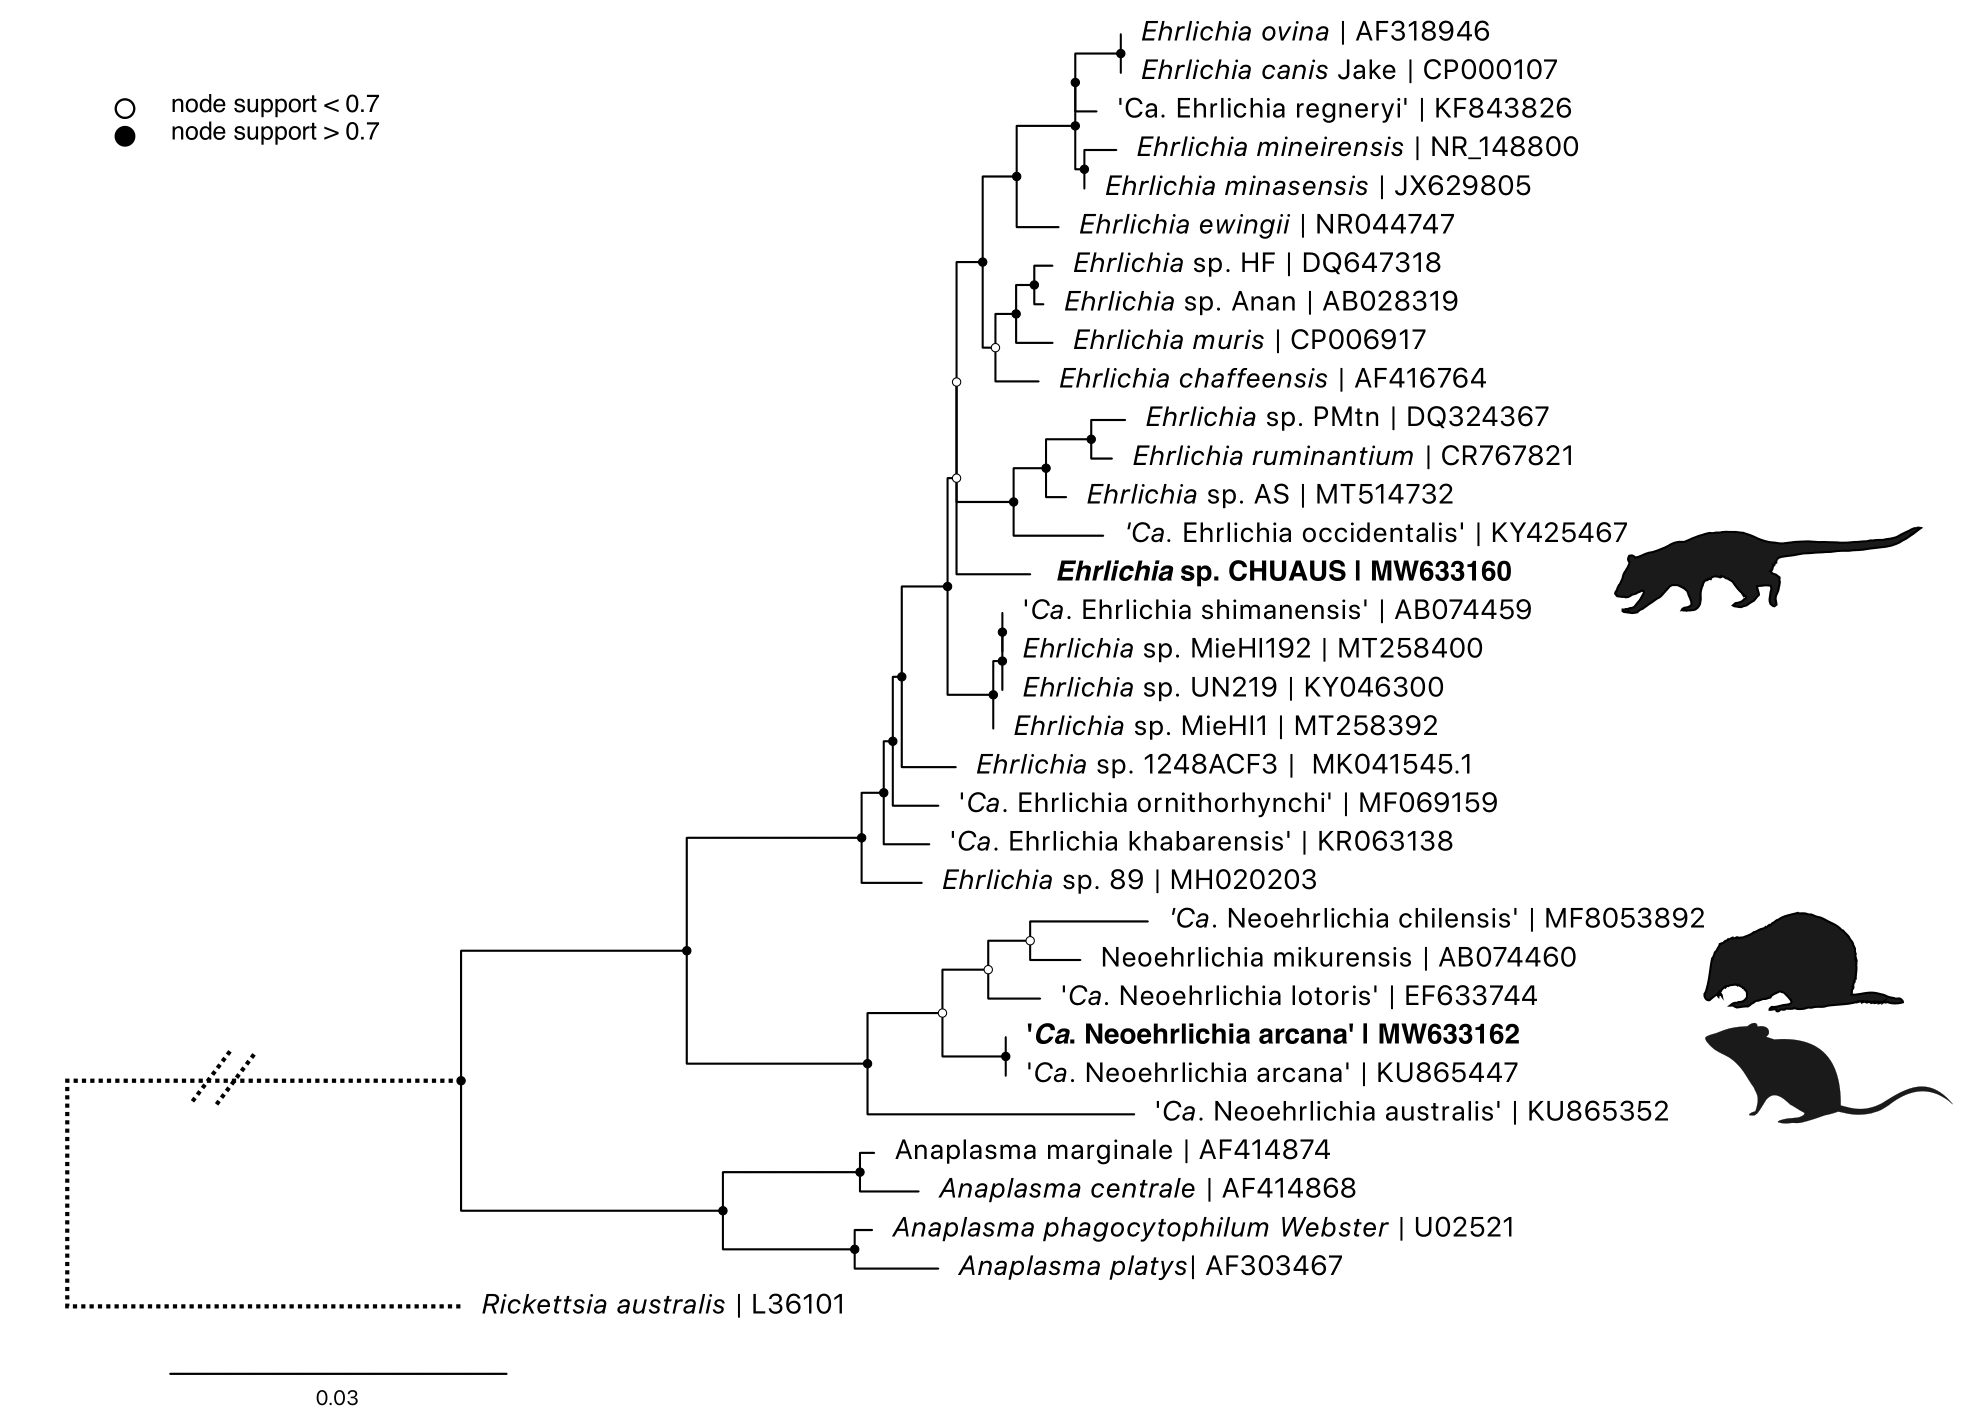
\includegraphics[width=0.95\linewidth]{figures/ms-figs/Ch3-anaplasmataceaetree} \caption[Phylogeny of \textit{Anaplasmataceae} species.]{Maximum likelihood (ML) phylogenetic reconstruction of \textit{Anaplasmataceae} based on a 1,244 bp alignment of the 16S rRNA locus. Substitution model K80 + F with 10,000 replicates. Node values correspond to bootstrap support where values > 0.7 are indicated by shaded circles. Number of substitutions per nucleotide position is represented by the scale bar. Sequences generated in the present study are in bold.}\label{fig:F3anaplas}
\end{figure}

\hypertarget{midichloria}{%
\subsubsection{\texorpdfstring{\emph{Midichloria}}{Midichloria}}\label{midichloria}}

A total of 103 samples were positive for \emph{Midichloria} which were identified in 94 tick samples from 62 individual animals.
Positive tick species included \emph{Ix. holocyclus}, \emph{Ix. tasmani}, \emph{Ix. trichosuri} from black rats, brown antechinuses, brush-tailed possums, long-nosed bandicoots and rabbits from New South Wales.
While \emph{Midichloria} was identified in 13 \emph{Ix. tasmani}, the relative abundance was low (108--363 sequences; 0.1-0.4\% relative abundance).
Nine tissue samples (nine individuals) were positive for \emph{Midichloria} however the number of sequences was generally low (111--14,002) when compared to tick samples; hosts included black rats (five), a brush-tailed possum (one) and long-nosed bandicoots (two).
Only two individuals had positive tissue and tick samples, one brush-tailed possum and one long-nosed bandicoot.
\emph{Midichloria} was identified in all instars of \emph{Ix. holocyclus} but only female and nymph stages of \emph{Ix. trichosuri} (Figure \ref{fig:F3heatmaptick}).
No blood samples were positive for \emph{Midichloria} (Figure \ref{fig:F3heatmap}).

\hypertarget{coxiellaceae}{%
\subsubsection{\texorpdfstring{\emph{Coxiellaceae}}{Coxiellaceae}}\label{coxiellaceae}}

The \emph{Coxiellaceae} family was identified in 183 samples from 113 individuals. Eleven individuals had positive blood samples, although there was a relatively low number of sequences (100--2,819), from hosts including the black rat (seven), brush-tailed possum (one) and long-nosed bandicoot (three).
One hundred and six ticks from 88 individuals were positive; \emph{Am triguttatum} (one), \emph{Ix. tasmani} (90) \emph{Ix. holocyclus} (nine), and \emph{Ix. trichosuri}.
Fifty-seven individuals were positive for \emph{Coxiellaceae} in tissue samples, including the black rat (33), brush-tailed possum (two), bush rat (two) and long-nosed bandicoot (20).
Forty-five individuals had at least two sample types positive for \emph{Coxiellaceae}, and only two black rats had positive blood, tick and tissue samples.
All instars of \emph{Ix. tasmani} sampled (female, nymph, larva) were positive for \emph{Coxiellaceae}, but only female \emph{Ix. holocyclus} were positive.

\hypertarget{rickettsiaceae}{%
\subsubsection{\texorpdfstring{\emph{Rickettsiaceae}}{Rickettsiaceae}}\label{rickettsiaceae}}

\emph{Rickettsia} was identified exclusively in 24 tick samples from 22 individuals.
Positive samples from Western Australia were all identified as originating in \emph{Am. triguttatum} (three) from brush-tailed possums and quenda.
Ticks identified as positive from New South Wales were: \emph{Ix. holocyclus} (nine) from black rats and long-nosed bandicoots, \emph{Ix. tasmani} (15) from black rats, bush rats, long-nosed bandicoots and rabbits, and \emph{Ix. trichosuri} (three) from long nosed bandicoots.
No tissue or blood samples were positive for \emph{Rickettsia}.

\hypertarget{borrelia-2}{%
\subsubsection{\texorpdfstring{\emph{Borrelia}}{Borrelia}}\label{borrelia-2}}

A novel \emph{Borrelia} sp. was identified in nine tissue samples: seven black rats, one bush rat and one swamp rat. The identity of these \emph{Borrelia} sequences showed they were most similar to \emph{Borrelia} R57 (AY626138, 95.68--96.70\% similarity, \protect\hyperlink{supplementary-table-e1.3}{Supplementary Table E1.1}).
Corresponding blood and ticks from these individuals were negative and no other \emph{Borrelia} sequences were identified from any other samples.

Attempts to amplify and perform Sanger sequencing on the \emph{flaB} gene using pan-\emph{Borrelia} primers \autocite{lohNovelBorreliaSpecies2016} were unsuccessful.
Given these failed attempts and the small volume of gDNA from samples (tissue biopsy punch only 2 mm), an alternative approach was employed to amplify additional fragments of the \emph{16S rRNA} v3-4 hypervariable region on the Illumina MiSeq.

After bioinformatic analysis outlined above, a single ASV was generated from all nine samples.
Phylogeny was reconstructed using the maximum likelihood method (GTR + R model) based on 426 bp alignment of the 16S rRNA locus (hypervariable region v3-4) (Figure \ref{fig:F3borrelia}). The novel \emph{Borrelia} sequence showed 98.4\% similarity with \emph{Borrelia} sp. ALEPB216 (KF957671) from \emph{R. rattus} in California, U.S.A (genetic distances \protect\hyperlink{supplementary-table-e1.3}{Supplementary Table E1.3}). The next most similar sequences were \emph{Borrelia} sp. CA682 (KF957670, similarity 98.1\%) and \emph{Borrelia} sp. R57 (AY626138, similarity 97.6\%).
The topology showed these sequences formed a distinct `rodent' clade, basal to the three major groups currently described (Figure \ref{fig:F3borrelia}). The nearest named species was \emph{Borrelia theileri} (U38375, similarity 94.50\%).

\begin{figure}
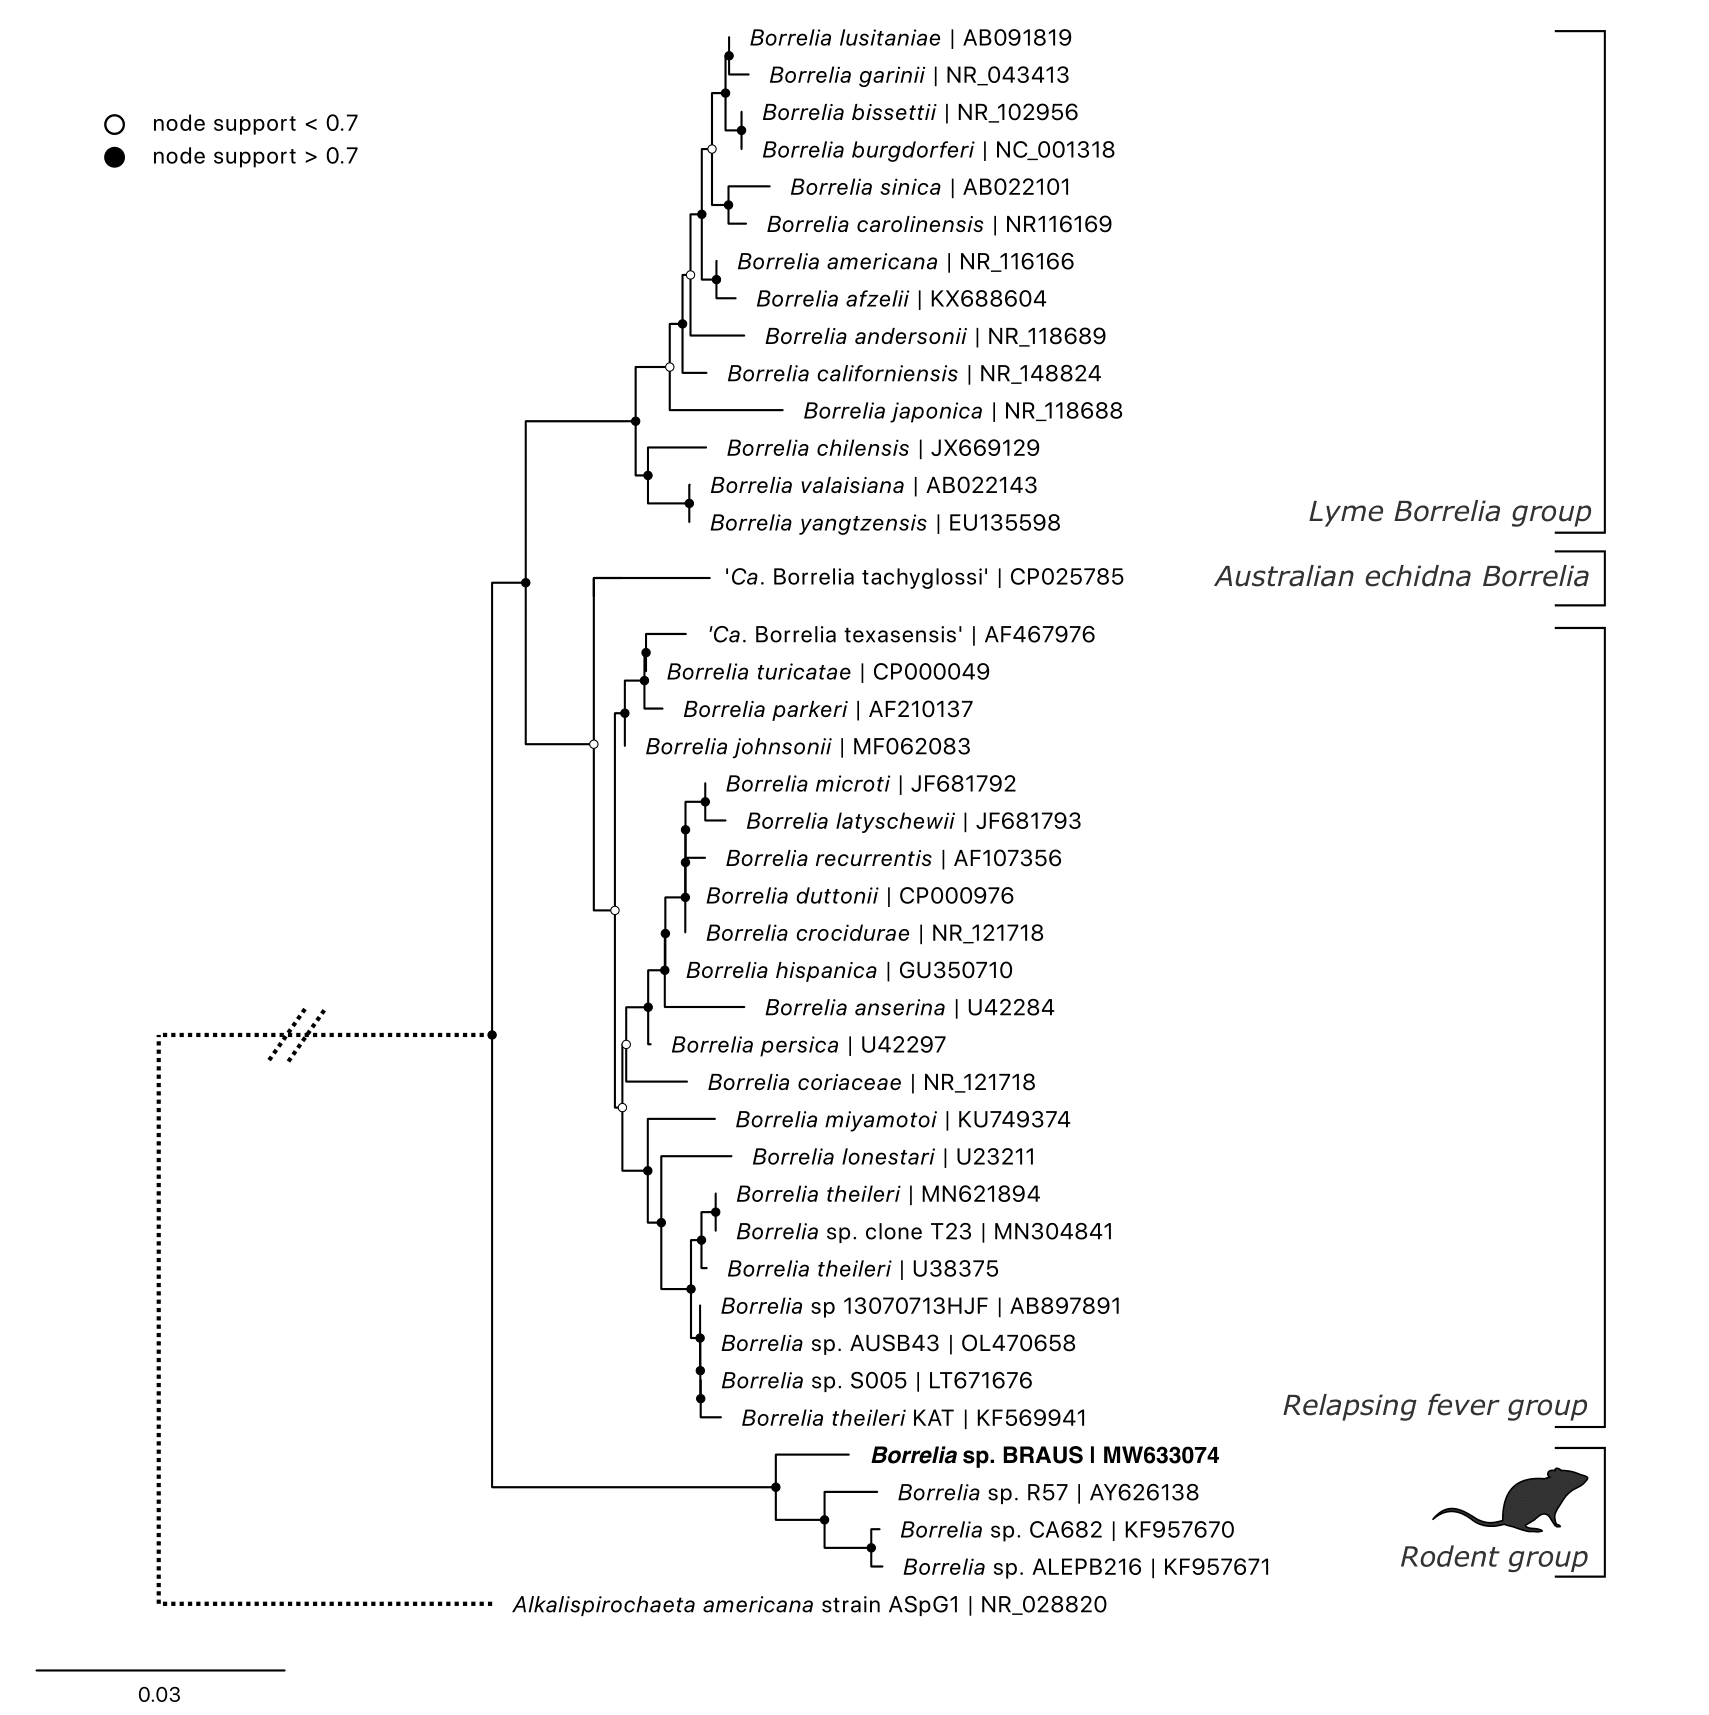
\includegraphics[width=0.95\linewidth]{figures/ms-figs/Ch3-borreliatree} \caption[Phylogeny of rodent \textit{Borrelia} species.]{Maximum likelihood (ML) phylogenetic reconstruction of \textit{Borrelia} genus based on a 431 bp alignment of the 16S rRNA locus (hypervariable region 3-4). Substitution model K2P + G4 with 10,000 replicates. Node values correspond to bootstrap support where values > 0.7 indicated by shaded circles. Number of substitutions per nucleotide position is represented by the scale bar. Sequence generated in the present study in bold.}\label{fig:F3borrelia}
\end{figure}

\hypertarget{bartonella}{%
\subsubsection{\texorpdfstring{\emph{Bartonella}}{Bartonella}}\label{bartonella}}

\emph{Bartonella} sp. was identified in 69 samples from 47 individuals. Blood samples represented the majority of \emph{Bartonella} positives with 35 individuals which included black rats (22), brush-tailed possums (seven), bush rats (two), and long-nosed bandicoots (four).
Nineteen individuals had positive tissue samples; black rats (four), brown antechinus (one), brush-tailed possums (nine), bush rats (two) and long-nosed bandicoots (three); seven individuals had positive tissue and blood samples.
Six tick samples were positive for \emph{Bartonella} (from five individuals) with three tick species (\emph{Ix. holocyclus}, \emph{Ix. tasmani} and \emph{Ix. trichosuri}) from black rats and long-nosed bandicoots. All tick samples that were positive also had corresponding positive blood or tissue samples.

Targeted sequencing on a subset of positive samples showed two genotypes of \emph{Bartonella queenslandensis} that were 97.2\% similar to each other with ten SNPs (genetic distances \protect\hyperlink{supplementary-table-e1.4}{Supplementary Table E1.4}.
The next most similar sequence to genotype BR025 and BR048 was \emph{Ba. queenslandensis} strain AUST/NH8 (EU111767) at 96.1\% and 94.8\% similarity respectively.
Comparison of \emph{Ba. queenslandensis} type sequences showed divergence up to 7.2\%\% (between EU111765 and EU111766) within the species. Five genotypes of \emph{Ba. coopersplainsensis} were identified with 94.4--99.2\% similarity to each other; and between 96.7--98.7\% similarity to \emph{Ba. coopersplainsensis} type sequence (EU111770) (Figure \ref{fig:F3bartonella}).

\begin{figure}
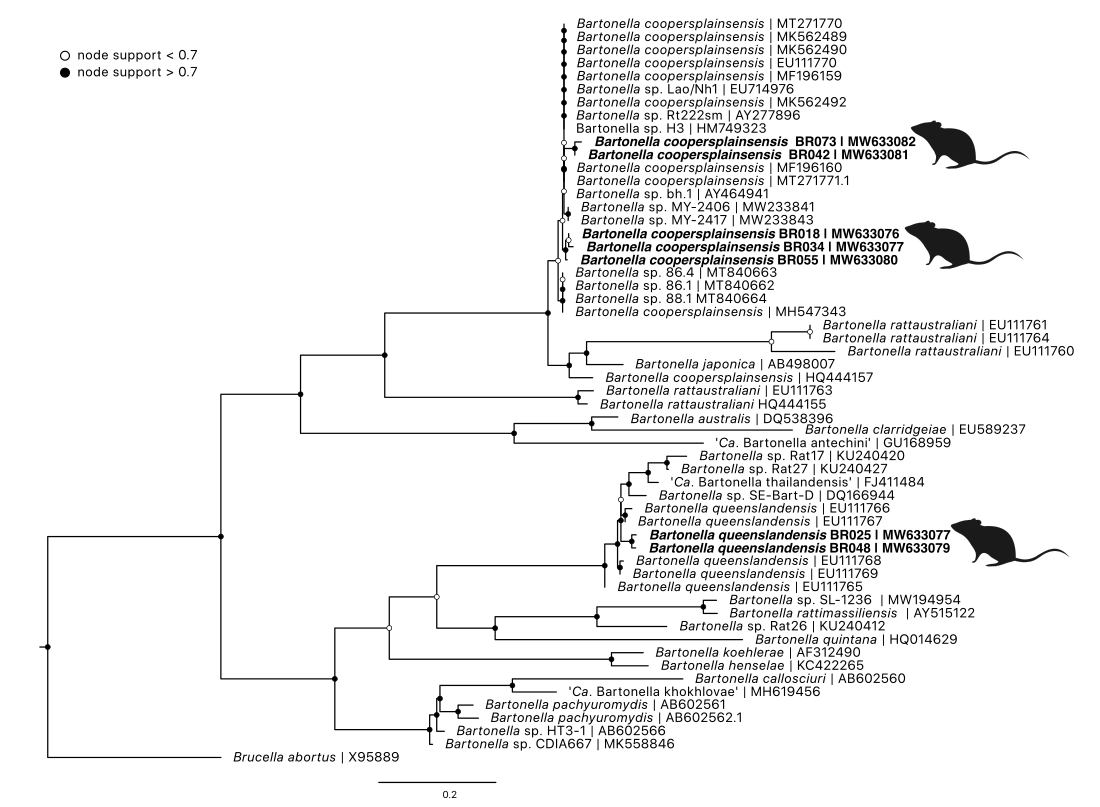
\includegraphics[width=0.95\linewidth]{figures/ms-figs/Ch3-bartonellatree} \caption[Phylogeny of  \textit{Bartonella} species.]{Maximum likelihood (ML) phylogenetic reconstruction of \textit{Bartonella} genus based on a 533 bp alignment of the 16S-23S internal transcribed space (ITS) region. Substitution model HKY + F with 10,000 replicates. Node values correspond to bootstrap support where values > 0.7 indicated by shaded circles. Number of substitutions per nucleotide position is represented by the scale bar. Sequences generated in the present study in bold.}\label{fig:F3bartonella}
\end{figure}

\hypertarget{francisella-and-mycoplasma}{%
\subsubsection{\texorpdfstring{\emph{Francisella} and \emph{Mycoplasma}}{Francisella and Mycoplasma}}\label{francisella-and-mycoplasma}}

\emph{Francisella} was identified in four ticks, \emph{Am. triguttatum} (three) and \emph{Ix. australiensis} (one) from brush-tailed possums and quenda in Western Australia (Table \ref{tab:T3prev}, \protect\hyperlink{supplementary-table-e1.1}{Supplementary Table E1.1}).
\emph{Mycoplasma} was present in three samples, from three individuals: two blood samples from a black rat and a swamp rat and one tissue sample from a black rat (Table \ref{tab:T3prev}, \protect\hyperlink{supplementary-table-e1.1}{Supplementary Table E1.1}).

\hypertarget{discussion}{%
\section{Discussion}\label{discussion}}

This body of work represents the first large scale investigation into tick (and vector)-associated bacteria concurrently with their vertebrate hosts in urban and peri-urban locations, and identified novel tick-associated bacteria in Australian wildlife.
Bacterial amplicon sequencing showed that there were limited taxa shared between blood, tick and tissue samples.
The identification of bacterial taxa of interest was generally confined to certain hosts and/or sample types.
To the best of the authors' knowledge, this study represents the first report of \emph{Neoehrlichia} and \emph{Ehrlichia} from Australian wildlife (blood and/or tissue samples).
The first identification of the rodent-associated \emph{Borrelia} clade in Australia is also described.
These findings show that geographic boundaries and host associations influence the prevalence of tick-associated bacteria.
Importantly, these findings also provide support for the absence of northern hemisphere tick-borne pathogens, adding to the overwhelming body of evidence that any potential human tick-borne pathogens in Australia are likely endemic and genetically distinct from currently described pathogens in parts of North America and Europe.

Although a comparatively deep level of sequencing was achieved compared to similar studies \autocite{rynkiewiczConcordanceBacterialCommunities2015,geSpleenMicrobiotaSmall2018}, rarefaction plots showed that blood samples did not reach the same asymptote as tick and tissue, indicating that deeper sequencing of these samples is needed to ensure complete coverage of bacterial diversity.
Across all four alpha diversity measures, tissue samples showed the highest diversity and variance.
In comparison, tick samples showed a less diverse bacterial composition.
This is likely due to the dominance of endosymbiont bacteria in the tick microbiome, which has been demonstrated in previous studies of the same tick species as identified in the present study \autocite{goftonInhibitionEndosymbiontCandidatus2015,eganBacterialCommunityProfiling2020}, and in tick species globally \autocite{lalzarCompositionSeasonalVariation2012,gilIxodesScapularisMicrobiome2020}.
The overall lack of similarity in bacterial communities between sample types observed in the present work has been reported in previous studies on small mammals and their vectors (ticks and fleas), indicating the complexity of microbial assemblages inhabiting these biological niches \autocite{cohenSimilaritiesSeasonalVariations2015,rynkiewiczConcordanceBacterialCommunities2015,liStochasticProcessesGovern2018}.
The diagnostic value of \emph{16S rRNA} amplicon sequencing methods has not been thoroughly validated for tick-borne pathogens.
One study however showed that ticks which tested positive for \emph{Borrelia} using qPCR methods also had a high abundance of \emph{Borrelia} using amplicon bacterial metabarcoding \autocite{sperlingMicrobiomeCompositionBorrelia2020}.
Therefore, even though \emph{Ix. holocyclus} and \emph{Ix. tasmani} had abundant endosymbionts, and the presence of bacterial species in lower abundance cannot be ruled out completely, it is likely that our finding of the absence of some bacterial species here reflects the true situation.

The microbiome of \emph{Ix. holocyclus} and \emph{Ix. tasmani} was dominated by a limited number of highly abundant ASVs.
Other tick species, such as \emph{Ix. trichosuri} and \emph{Ix. australiensis}, showed a more diverse bacterial composition.
The interaction between bacterial endosymbionts and pathogens in ticks is not yet fully understood.
The presence of endosymbiont bacteria is thought to inhibit the colonisation by other potentially pathogenic bacterial species.
For example, colonisation by the rickettsial endosymbiont (\emph{Rickettsia peacockii}) in \emph{Dermacentor andersoni} tick ovaries is thought to render the ticks more resistant to co-infection by a second rickettsial species (\emph{Rickettsia rickettsii}), which is the main cause of Rocky Mountain Spotted Fever
\autocite{burgdorferNonpathogenicRickettsiaeDermacentor1981}
\autocite{burgdorferNonpathogenicRickettsiaeDermacentor1981,macalusoRickettsialInfectionDermacentor2002}.

Likewise, \emph{Dermacentor variabilis} ticks infected with one strain of \emph{Rickettsia} were shown to be less susceptible to secondary rickettsial infections \autocite{macalusoRickettsialInfectionDermacentor2002}.
However, this theory is not uniformly accepted, and there is some rejection of Burgdorfer's \autocite{burgdorferNonpathogenicRickettsiaeDermacentor1981} initial findings.
Instead, it is hypothesised that differences in \emph{R. peacockii} prevalence in \emph{De. andersoni} are due to microclimatic factors \autocite{telfordStatusEastSide2009}.
Additionally, in recent years microbiome profiling has led to conflicting conclusions about the interaction between endosymbiont and pathogens \autocite{bonnetUpdateIntricateTango2020}.
Based on what is known from the northern hemisphere examples, tick species without a dominant endosymbiont may pose a greater risk of harbouring potentially pathogenic microbes \autocite{bonnetUpdateIntricateTango2020}.

Equivalent studies from the northern hemisphere using \emph{16S rRNA} metabarcoding methods and wildlife surveillance to identify tick-borne pathogens are limited.
Instead, pathogen surveillance studies are generally targeted to well-known pathogens.
For example, studies of \emph{B. burgdorferi} sensu lato have shown infection is not detrimental to the health of natural rodent reservoirs \autocite{voordouwLymeDiseasePathogen2015}, which have been shown to harbour a diverse range of \emph{Borrelia} species \autocite{bunikisThirdBorreliaSpecies2005}.
In the present study, chuditch and long-nosed bandicoots had a high abundance of \emph{Anaplasmataceae} in blood samples, while brush-tailed possums had the highest abundance of this taxon in tissue samples.
In addition, \emph{Anaplasmataceae} bacteria were mostly absent from larval ticks.

This suggests that the \emph{Anaplasmataceae} bacteria identified are likely maintained via horizontal transmission (i.e.~between host and tick) and transstadial routes, which has been observed with related bacteria in companion animals \autocite{fourieTransmissionEhrlichiaCanis2013,almazanExperimentalIxodesRicinusSheep2020}.
In contrast, the identification of \emph{Midichloria} across all life stages of \emph{Ix. holocyclus} shows evidence of vertical (transovarial) transmission.
Both horizontal and vertical transmission have been identified previously in other tick species with \emph{Midichloria} \autocite{maricontiHumansParasitizedHard2012,serraMolecularSerologicalEvidence2018}.
The absence of \emph{Midichloria} in vertebrate hosts (blood and skin) in the present study suggests the horizontal infection route is not a major contributor to the presence of this endosymbiont in \emph{Ix. holocyclus} and is consistent with previous studies \autocite{mukhachevaBacteriaFamilyCandidatus2017}.

\hypertarget{taxa-of-interest-1}{%
\subsection{Taxa of interest}\label{taxa-of-interest-1}}

\hypertarget{anaplasmataceae-3}{%
\subsubsection{\texorpdfstring{\emph{Anaplasmataceae}}{Anaplasmataceae}}\label{anaplasmataceae-3}}

The present study has provided the first identification of \emph{Neoehrlichia} spp. from Australian wildlife. Two \emph{Neoehrlichia} species, `\emph{Ca}. N. arcana' and `\emph{Ca}. N. australis', were recently characterised from \emph{Ix. holocyclus} along the east coast of Australia at a prevalence of 11.3\% (44/391) \autocite{goftonPhylogeneticCharacterisationTwo2016}.
This finding is consistent with other species of \emph{Neoehrlichia} globally, which have been described circulating in a range of mammals and associated ticks \autocite{kawaharaUltrastructurePhylogeneticAnalysis2004,mullerCandidatusNeoehrlichiaChilensis2018}.
In contrast to Gofton et al. \autocite*{goftonPhylogeneticCharacterisationTwo2016}, the results presented here show that `\emph{Ca}. N. arcana' is more prevalent than `\emph{Ca}. N. australis' in small mammals, which is consistent with a recent study of Australian wildlife ticks \autocite{eganBacterialCommunityProfiling2020}.
The main reservoir host for `\emph{Ca}. N australis' is likely to be medium to large macropods (e.g.~eastern grey kangaroo (\emph{Macropus giganteus}) or swamp wallaby (\emph{Wallabia bicolor})), which were not sampled in the present study.

The identification of three putative novel \emph{Anaplasmataceae} species further demonstrates the high diversity of \emph{Anaplasmataceae} from Australian ticks and wildlife.
This finding adds to recent discoveries identifying new species from \emph{Am. triguttatum} \autocite{goftonDetectionPhylogeneticCharacterisation2017}, \emph{Bothriocroton concolor}, \autocite{lohIdentificationCharacterisationMicroorganisms2018}, \emph{Ix. holocyclus} \autocite{goftonPhylogeneticCharacterisationTwo2016}, and from the platypus (\emph{Ornithorhynchus anatinus}) and its associated ticks \emph{Ix. ornithorhynchi} \autocite{goftonNovelEhrlichiaSpecies2018}.
The novel \emph{Anaplasmataceae} species were less readily identified in tick vectors compared to `\emph{Ca}. N. arcana' and `\emph{Ca}. N. australis'; however more targeted studies are needed to understand their prevalence and distribution.

The first identification of \emph{Anaplasma platys} (formerly \emph{Ehrlichia platys}) in Australia was made in 2001 \autocite{brownDetectionEhrlichiaPlatys2001}, and has since been described from dogs throughout the country \autocite{brownDetectionAnaplasmaPlatys2006,hiiCanineVectorborneDisease2012}.
To date it has not been identified in any native Australian wildlife, although \emph{Anaplasma platys} has been reported from deer overseas \autocite{yuPrevalenceCommonTickborne2020}.
To the best of the authors' knowledge, this is the first report of \emph{A. platys} from wild deer in Australia. The vector of \emph{A. platys} overseas, \emph{Rhipicephalus sanguineus} \autocite{snellgroveVectorCompetenceRhipicephalus2020}, is likely also the vector in Australia.
The brown dog tick, syn. \emph{Rh. sanguineus} tropical lineage was recently named \emph{Rhipicephalus linnaei} \autocite{slapetaTropicalLineageBrown2021}. Importantly, \emph{Ehrlichia canis}, which was first identified in dogs and brown dog ticks in northern Australia during 2020, was not identified in ticks, tissue or blood from wildlife in this study.

\hypertarget{midichloria-1}{%
\subsubsection{\texorpdfstring{\emph{Midichloria}}{Midichloria}}\label{midichloria-1}}

While `\emph{Ca}. M. mitochondrii' (CMm) is known to be highly prevalent and abundant in ticks identified in the present study, the present study did not employ a blocking primer as used in previous studies \autocite{goftonInhibitionEndosymbiontCandidatus2015,eganBacterialCommunityProfiling2020}.
The justification for this was a deliberate choice to include CMm in the `taxa of interest' investigation, i.e.~provide insight into the ecology of this microbe.
The absence of CMm in both blood and tissue was surprising, especially given the high proportion and abundance of the bacteria in \emph{Ix. holocyclus} in the present study.
Studies in France have identified CMm from roe deer blood samples (\emph{Capreolus capreolus}) using molecular and serology techniques \autocite{serraMolecularSerologicalEvidence2018}; while that study reported a higher sensitivity for serology, molecular methods were also successful at identifying infection.
In vitro studies of \emph{Ix. ricinus} and rabbits suggest that the endosymbiont replicates within the vertebrate host \autocite{cafisoMidichloriaMitochondriiEndosymbiont2019}.
The bacterial microbiome of many tick species is generally dominated by the presence of one (or a few) highly abundant endosymbiont microbes \autocite{claytonCharacterizationManipulationBacterial2015,goftonInhibitionEndosymbiontCandidatus2015,varela-stokesMicrobialCommunitiesNorth2017}.
This suggests that rare, less abundant bacteria are not easily identified using standard \emph{16S rRNA} bacterial metabarcoding methods.
While the possibility cannot be ruled out, given the high abundance of CMm in tick samples, it is likely that the methods employed here would have identified it in wildlife hosts (either blood or tissue) if present.
Therefore, given the absence of CMm in the hosts sampled in the present study, vertical transmission may be the primary source of \emph{Midichloria} infection for \emph{Ix. holocyclus}. Alternatively, the reservoir host for CMm may not have been sampled.

\hypertarget{coxiellaceae-1}{%
\subsubsection{\texorpdfstring{\emph{Coxiellaceae}}{Coxiellaceae}}\label{coxiellaceae-1}}

All \emph{Coxiellaceae} ASVs identified were most similar to members of the \emph{Rickettsiella} genus and dominated the microbiome of \emph{Ix. tasmani}.
\emph{Coxiella} was not detected in the present study.
The absence of \emph{Coxiella} from host blood and tissue samples likely reflects a low abundance of this bacteria in the small mammal hosts sampled.
Serological methods are more commonly used to detect exposure to \emph{C. burnetii} \autocite{cooperSerologicalEvidenceCoxiella2012} but lack the ability to detect acute infections.
A recent study using molecular techniques detected \emph{C. burnetii} in kangaroo meat samples \autocite{shapiroMolecularDetectionCoxiella2020}. This suggests that animals sampled in the present study were negative for an active infection with \emph{Coxiella}.

\hypertarget{rickettsiaceae-1}{%
\subsubsection{\texorpdfstring{\emph{Rickettsiaceae}}{Rickettsiaceae}}\label{rickettsiaceae-1}}

While several forms of rickettsiosis are amongst the few recognised human tick-borne diseases in Australia, remarkably little is known about the sylvatic life cycle of these intracellular bacteria.
At least five agents of human rickettsial disease have been described in Australia \autocite{tadepalliMolecularEvidenceNovel2021}, together with several additional species and genotypes with unknown pathogenicity \autocite{vilcinsDetectionSpottedFever2008,vilcinsEvidencePresenceFrancisella2009,tadepalliMolecularEvidenceNovel2021}.
Bandicoots and other small mammals have previously been described as reservoirs for Queensland tick typhus (\emph{R. australis}), and \emph{Ix. holocyclus} and \emph{Ix. tasmani} are known vectors \autocite{campbellRickettsiosesAustraliaIsolation1974,sextonSpottedFeverGroup1991}.
Although the relationship between bandicoots and rickettsial infections is largely accepted there has been little validation of this association since the early publications.

In the present study, the genus \emph{Rickettsia} was predominately identified from ticks, with a low prevalence and abundance in four tissue samples and was absent from all blood samples.
Areas sampled in Sydney's northern beaches are endemic for Queensland tick typhus and spotted fever.
Therefore, the absence of spotted fever or typhus group \emph{Rickettsia} from mammal hosts in the present study was unexpected.
Recent studies utilising qPCR have reported \emph{Rickettsia} in 15.4\% (23/149) \emph{Ix. holocyclus} from NSW \autocite{gravesIxodesHolocyclusTicktransmitted2016} and 6.4\% (13/203) ticks collected from wildlife in north-east Queensland \autocite{hussain-yusufScreeningRickettsiaCoxiella2020}.
Additional reports also recognise the presence of spotted fever group \emph{Rickettsia} in Australian ticks \autocite{cookScrubTyphusOther1967,campbellRickettsiosesAustraliaIsolation1974,gravesRickettsiosesAustralia2006}.

The lack of \emph{Rickettsia} identified in ticks may be due to the highly abundant endosymbionts \emph{Midichloria} or Coxiellaceae in \emph{Ix. holocyclus} and \emph{Ix. tasmani} respectively.
While there are limited comparable studies that have used bacterial metabarcoding on wildlife blood samples, previous research has shown that molecular methods successfully identify \emph{Rickettsia} in reservoir hosts \autocite{ndeerehMolecularSurveillanceSpotted2017,martelloBorreliaBurgdorferiSensu2019,chaorattanakaweeAmpliconBasedNextGeneration2021}. Flinders Island Spotted Fever, caused by \emph{R. honei} is associated with reptiles and the southern reptile tick \emph{Bo. hydrosauri} \autocite{stenosAponommaHydrosauriReptileassociated2003}.
A closely related strain, named \emph{R. honei marmionii}, has been identified from various regions in Australia and is associated with \emph{Haemaphysalis novaeguineae} \autocite{laneEvidenceSpottedFeverlike2005a,unsworthFlindersIslandSpotted2007}.
Interestingly no \emph{Haemaphysalis} ticks were identified from hosts in the present study.
Further investigation into the sylvatic cycle of \emph{Rickettsia} in Australia would benefit from the inclusion of samples from reptile hosts and vertebrate hosts of \emph{Haemaphysalis} ticks.

\hypertarget{borrelia-3}{%
\subsubsection{\texorpdfstring{\emph{Borrelia}}{Borrelia}}\label{borrelia-3}}

The novel \emph{Borrelia} identified here came exclusively from black rats and was found at two sites in Sydney's Northern Beaches area. All samples that tested positive were tissue, and no \emph{Borrelia} sequences were identified from corresponding blood or tick samples.

The \emph{Borrelia} species identified from black rats formed a clade with other described \emph{Borrelia} species identified from rodents. \emph{Borrelia} sp. R57 was identified from bank voles (\emph{Myodes glareolus}; formerly \emph{Clethrionomys glareolus}) and wood mice (\emph{Apodemus sylvaticus}) in Spain at a prevalence rate of 8.5--12.0\% using PCR methods \autocite{gilIdentificationNewBorrelia2005}.
That study identified serological cross-reactivity of this species with \emph{B. burgdorferi} sensu lato using western blot testing.
A follow-up study (in Spain) further identified the genotype from 24.5\% (62/253) of rodent tissue samples \autocite{barandikaTickBorneZoonoticBacteria2007}.
Identification of similar sequences was subsequently made from black rats (\emph{R. rattus}) in California, U.S.A., with a prevalence of 43.5\% (10/23) in tissue (skin) biopsy samples \autocite{fedorovaRemarkableDiversityTick2014}.
The absence of this \emph{Borrelia} species from our tick samples is interesting and mirrors the previous studies in Europe and the U.S.A \autocite{gilIdentificationNewBorrelia2005,fedorovaRemarkableDiversityTick2014}.
Despite multiple attempts during this study, amplification at the \emph{flaB} locus was unsuccessful, consistent with previous research of members within the clade \autocite{gilIdentificationNewBorrelia2005}.

The extensive geographical range of this clade, yet tight host associations identified to date (i.e.~confined to the Order Rodentia), raises questions regarding its origin.
Particularly interesting is the paucity of reports globally, despite small mammals being the most widely studied reservoir host of tick-borne diseases \autocite{zikeliWhyResearchLyme2020}.
Our phylogenetic analysis shows strong support for these \emph{Borrelia} sequences forming a distinct clade and is consistent with other studies \autocite{margosControversiesBacterialTaxonomy2019}.
Its basal phylogenetic position may provide important insights into the evolutionary history of the \emph{Borrelia} genus.
The lack of its identification in tick samples means that the vector for this \emph{Borrelia} sp. remains unknown, and the transmissibility and pathogenicity of this microbe requires further research.
Importantly, no identifications were made of the recently characterised \emph{Borrelia} species from Australia, `\emph{Ca}. B. tachyglossi' \autocite{lohMolecularCharacterizationCandidatus2017} or reptile \emph{Borrelia} sp. \autocite{panettaReptileassociatedBorreliaSpecies2017}, nor any sequences from the \emph{B. burgdorferi} sensu lato group.

Currently there is no evidence that the novel rodent-associated \emph{Borrelia} genotype identified in the present study is transmissible to humans or capable of causing disease.
Phylogenetic reconstruction indicates that it is distinct from the \emph{B. burgdorferi} sensu lato and relapsing fever groups \autocite{margosControversiesBacterialTaxonomy2019}.
The absence of detection from tick samples and its identification only in rodents, more likely implies another vector that presumably has a tight host relationship with \emph{Rattus} species.

\hypertarget{bartonella-1}{%
\subsubsection{\texorpdfstring{\emph{Bartonella}}{Bartonella}}\label{bartonella-1}}

\emph{Bartonella} spp. was identified in a relatively high proportion of wildlife blood samples, and most prevalent in blood samples from black rats (31.0\%).
\emph{Bartonella coopersplainsensis} and \emph{Ba. queenslandensis} were described from native Australian rodents (\emph{Melomys} spp. and \emph{Rattus} spp.) in Queensland \autocite{gundiBartonellaRattaustralianiSp2009}.
Since then, a number of novel \emph{Bartonella} strains have been identified from Australia, including novel species described from marsupials and their ectoparasites (ticks and fleas) \autocite{vilcinsBartonellalikeDNADetected2009,kaewmongkolCandidatusBartonellaAntechini2011,kaewmongkolGeneticCharacterizationFleaderived2011}.
While generally considered to be transmitted by fleas, reports of \emph{Bartonella} species isolated from ticks are increasing, as studies take a broader approach to surveillance of vector-associated microbes \autocite{rynkiewiczConcordanceBacterialCommunities2015,asyikhaDetectionBartonellaSp2020,krolEvaluatingTransmissionPaths2021}.
Identification of \emph{Bartonella} in fed ticks does not mean they are a viable vector, but it does highlight that future studies should include ticks when exploring candidate vectors.
The high identification of \emph{Bartonella} in rodents has been reported in other metabarcoding studies from blood samples \autocite{cohenSimilaritiesSeasonalVariations2015}.

\hypertarget{francisella-and-mycoplasma-1}{%
\subsubsection{\texorpdfstring{\emph{Francisella} and \emph{Mycoplasma}}{Francisella and Mycoplasma}}\label{francisella-and-mycoplasma-1}}

\emph{Francisella} was identified exclusively from ticks in Western Australia, \emph{Am. triguttatum} and \emph{Ix. australiensis}.
Previous bacterial profiling of \emph{Am. triguttatum} has shown a high proportion of \emph{Francisella} species \autocite{goftonBacterialProfilingReveals2015,eganBacterialCommunityProfiling2020}.
Given its high abundance in tick samples, the absence of \emph{Francisella} in corresponding host may indicate a lack of transmission.
Tularemia (caused by \emph{Francisella tularensis}) can cause disease in humans and animals.
While the infection is more commonly acquired via handling infected animal material or aerosol inhalation, \emph{F. tularensis} has been reported in ticks \autocite{regierCombinationMicrobiomeAnalysis2019}.
\emph{Francisella} has been reported in several tick species \autocite{garcia-vozmedianoDermacentorMarginatusDermacentor2020}.
While the species identified in the present study is not closely related to \emph{F. tularensis}, considering the significance of this genera \autocite{regierCombinationMicrobiomeAnalysis2019}, further characterisation should be of high importance.

The present study did not identify any haemoprotic \emph{Mycoplasma} species. The \emph{Mycoplasma} sequences identified were most closely related to \emph{Mycoplasma arthritidis}, which is recognised as a common pathogen in rats \autocite{dybvigGenomeMycoplasmaArthritidis2008}.
It was identified in two black rats and a single identification in the native swamp rat.

\hypertarget{limitations-and-recommendations}{%
\subsection{Limitations and recommendations}\label{limitations-and-recommendations}}

While the cost of \hl{high-throughput sequencing} platforms continues to decline, analysis of large numbers of samples is still constrained by resources and funds.
Amplicon high throughput sequencing remains a cost-effective approach for characterising bacterial microbiomes.
With the advent of long-read sequencing technologies (e.g.~PacBio), more studies are moving towards obtaining full-length \emph{16S rRNA} sequences which allow for more robust phylogenetic reconstruction and in many cases identification of bacteria to strain/genotype level \autocite{earlSpecieslevelBacterialCommunity2018,callahanHighthroughputAmpliconSequencing2019}.
In addition to describing the bacteria present, the idea of the functional tick microbiome has been suggested \autocite{estrada-penaTaxonomicVariabilityFunctional2020}.
While adaption of these methods can seem promising, their use outside of human microbiome studies is questionable due to the reliability of databases \autocite{bonnetUpdateIntricateTango2020,sunInferencebasedAccuracyMetagenome2020}.
An alternative approach such as the ``common core'' or ecological ``core microbiome'' may be more suitable in the context of tick microbiome research \autocite{riselyApplyingCoreMicrobiome2020}.
Studies incorporating transcriptomics will likely also prove useful for understanding the functional components of the microbiome.

While the present study reported on the relative abundance of microbes between ticks sampled, it is well known that differences in the 16S copy number limit inferences \autocite{brooksTruthMetagenomicsQuantifying2015,loucaCorrecting16SRRNA2018}.
In the context of the present study, relative abundance of taxa was compared among samples, as it was considered a suitable measure given samples were processed in the same manner.
Calculations of absolute abundance using \emph{16S rRNA} metabarcoding are challenging. While copy number is one factor that can be modelled it relies on information that in many cases is not accurately known.
Using mock communities can help assess bias without baseline data on copy number, however, these analysis methods are still limited.

The sensitivity of molecular diagnostic testing for tick-borne pathogens has been shown to vary greatly.
Factors that can influence molecular detection of pathogens include level of parasitaemia/bacteremia, sample type, time of sample collection from initial infection, and and pre-analytical preparation techniques; additionally, this is compounded by differences between taxa due to host-pathogen interactions \autocite{delafuenteTickPathogenInteractionsVector2017,estrada-penaFunctionalRedundancyEcological2017,bonnetEditorialTickHostPathogenInteractions2018}.
A strong advantage of using generic metabarcoding assays is their unbiased approach; in the context of the present study, the most important factor was to achieve unbiased characterisation of bacterial communities from Australian wildlife.
However, it is acknowledged that the use of bacterial metabarcoding for the identification of low abundant and rare organisms is limited.
The lack of recognised endemic bacterial pathogens such as \emph{Coxiella burnetii}, and \emph{Rickettsia} spp. was surprising.
Future studies should use serological and culture methods in addition to these highly specific and sensitive molecular tools (e.g.~qPCR).

Another limitation of the present study was the bias in animals sampled.
Small mammals were chosen as it was hypothesised they would have the highest prevalence of potential tick-borne pathogens based on what is known from the northern hemisphere \autocite{bastianAntibodyPrevalenceMolecular2012,bouchardHarvestedWhitetailedDeer2013,sweiEvidenceTransmissionZoonotic2019}.
Further sampling with expanded host and spatial aspects are vital to understand the full epidemiology of tick (and vector) associated microbes. Likewise, alternative trapping methods (e.g., differing trap type, bait) may expand the suite of hosts captured, importantly those with territorial overlap (e.g., semi-arboreal marsupials).

In the present study, most taxa of interest were confined to specific sample types. For example, \emph{Borrelia} was identified from tissue samples of rats but absent from any blood or tick samples.
This finding has also been reported in white-footed mice (\emph{Peromyscus leucopus}) \autocite{zawadaOptimizationTissueSampling2020}.
While in many cases disease surveillance is targeted to known pathogens where sampling protocols and diagnostics are well defined, in scoping studies such as the present one, a range of sample types are essential.
This is evident in the different ways pathogens act within their host.
As the first line of defense, the innate immune system has a key role in protecting against cutaneous and systemic infection \autocite{coatesInnateAntimicrobialImmunity2018}.
Alternatively pathogens can quickly evade host innate immune responses by rapidly disseminating into the blood stream after invasion \autocite{kumarIntravitalImagingVascular2015,hydeBorreliaBurgdorferiKeeps2017}.
In the context of Australia however, many wildlife species are endangered and therefore their capture and sampling in the wild is subject to strict ethical conditions and government regulations.
As such, collection of multiple sample types is restricted to those requiring only a minimally invasive method and is also dependent on the availability of trained personnel and resources.
In many instances it is standard procedure to collect a tissue biopsy for animal genetic (population) purposes, this presents a simple alternative to other procedures which may require field anaesthesia.
The results here highlight the value of this sample type for use in pathogen surveillance.

\hypertarget{conclusions}{%
\section{Conclusions}\label{conclusions}}

Increased land-use and climate change will continue to affect the spread of vectors and associated diseases globally.
There is an urgent need for expanded disease surveillance, particularly at the urban interface with wildlife.
Through collaborative approaches, discoveries of novel microbes and important epidemiological links will be critical to ensure adequate and timely responses to human and animal diseases.
Investigations into taxa of interest in the present study showed \emph{Anaplasmataceae} bacteria had a relatively high prevalence in the vertebrate hosts examined here and a wide geographical distribution.
This group of bacteria is therefore a viable candidate for continued research into Australian zoonotic tick-borne diseases.

\hypertarget{wildlife-haemoprotozoa}{%
\chapter{Haemoprotozoa surveillance}\label{wildlife-haemoprotozoa}}

\chaptermark{Haemoprotozoa}

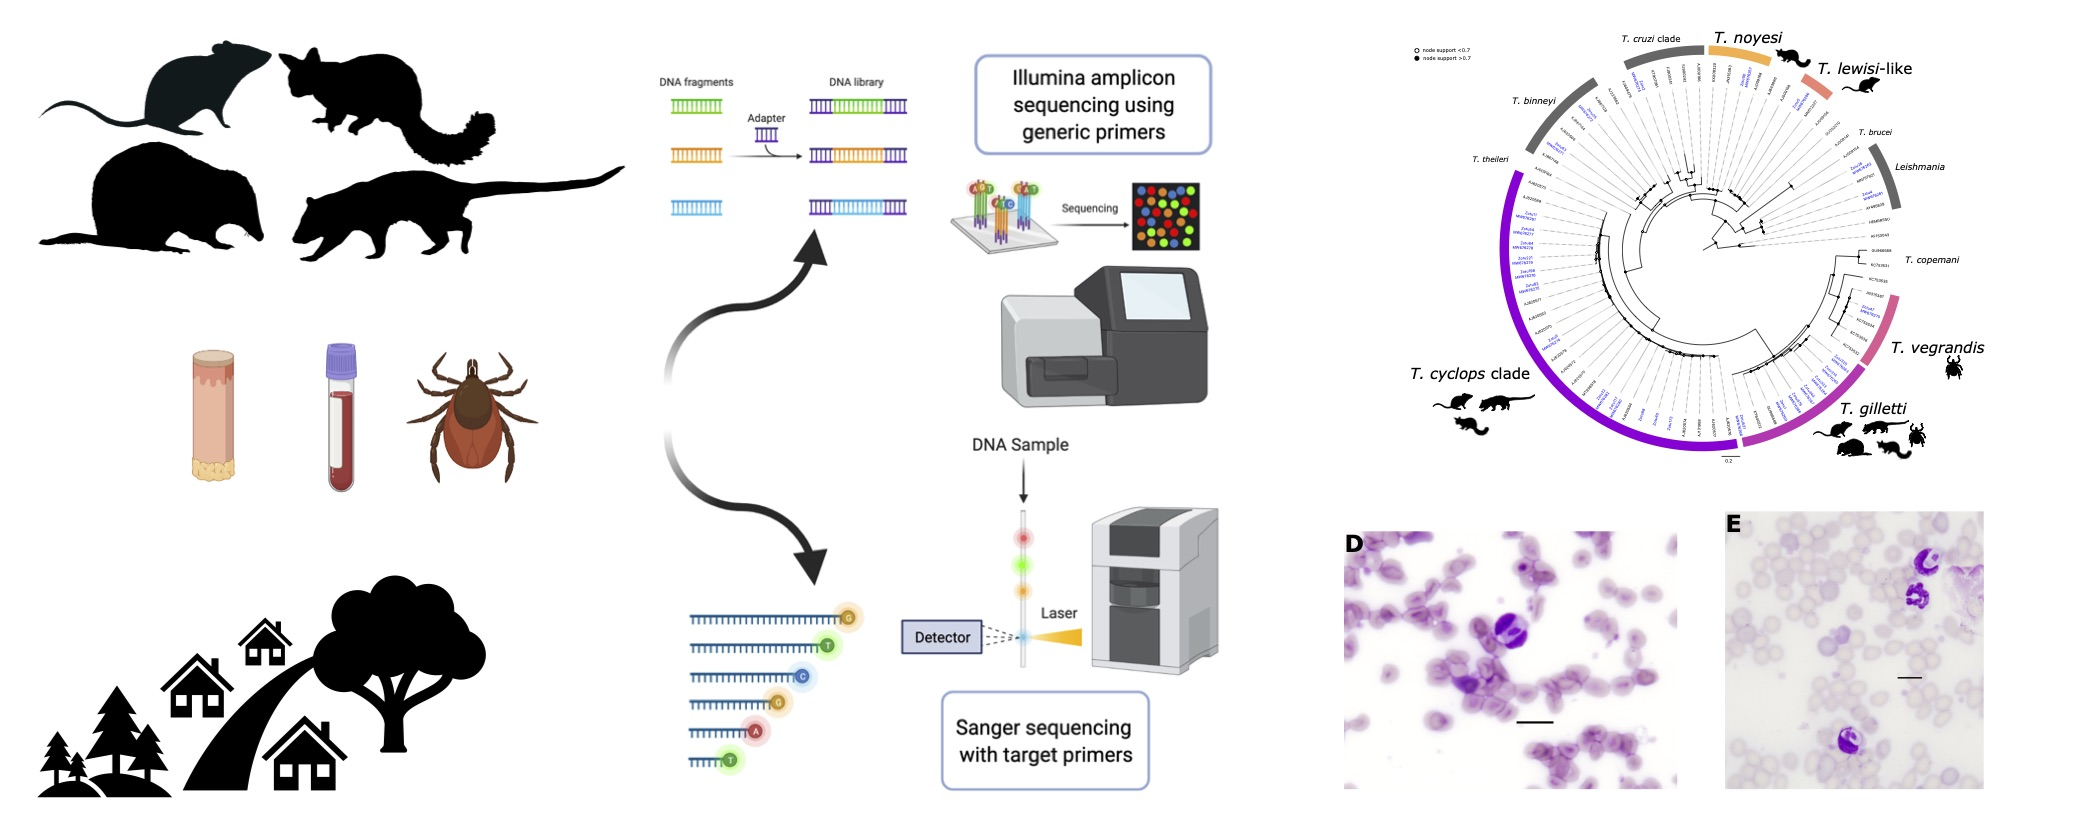
\includegraphics[width=1\linewidth]{front-and-back-matter/preface/haemoprotozoa}

\newpage

\hypertarget{preface-3}{%
\section*{Preface}\label{preface-3}}
\addcontentsline{toc}{section}{Preface}

\textbf{Attribution Statement}

The following chapter has been drafted in accordance with the journal \emph{Current Research in Parasitology and Vector-Borne Diseases}.

The following manuscript has been published: \textbf{Egan, S.}, Taylor, C., Austen, J., Banks, P., Northover, A., Ahlstrom, L., Ryan, U., Irwin, P., and Oskam C. Haemoprotozoan surveillance in peri-urban native and introduced wildlife from Australia. \emph{Current Research in Parasitology and Vector-Borne Diseases}, \textbf{1}, 100052. DOI: \href{https://doi.org/10.1016/j.crpvbd.2021.100052}{10.1016/j.crpvbd.2021.100052}

The following authors contributed to this manuscript as outlined below\footnote{Contribution indicates the total involvement the author has had in this project. Placing an `X' in the remaining boxes indicates what aspect(s) of the project each author engaged in.}.

\begin{table}[!h]
\centering\begingroup\fontsize{7}{9}\selectfont

\begin{tabular}{lrllll}
\toprule
Authorship order & Contribution (\%) & Concept Development & Data Collection & Data Analysis & Draft\\
\midrule
\cellcolor{gray!6}{Siobhon L. Egan} & \cellcolor{gray!6}{70.0} & \cellcolor{gray!6}{X} & \cellcolor{gray!6}{X} & \cellcolor{gray!6}{X} & \cellcolor{gray!6}{X}\\
Casey L. Taylor & 5.0 &  & X &  & \\
\cellcolor{gray!6}{Jill M. Austen} & \cellcolor{gray!6}{2.5} & \cellcolor{gray!6}{} & \cellcolor{gray!6}{} & \cellcolor{gray!6}{X} & \cellcolor{gray!6}{}\\
Peter B. Banks & 2.5 & X &  &  & \\
\cellcolor{gray!6}{Amy S. Northover} & \cellcolor{gray!6}{2.5} & \cellcolor{gray!6}{} & \cellcolor{gray!6}{X} & \cellcolor{gray!6}{} & \cellcolor{gray!6}{}\\
Liisa A. Ahlstrom & 2.5 &  & X &  & \\
\cellcolor{gray!6}{Una M. Ryan} & \cellcolor{gray!6}{5.0} & \cellcolor{gray!6}{X} & \cellcolor{gray!6}{} & \cellcolor{gray!6}{} & \cellcolor{gray!6}{}\\
Peter J. Irwin & 5.0 & X &  &  & \\
\cellcolor{gray!6}{Charlotte L. Oskam} & \cellcolor{gray!6}{5.0} & \cellcolor{gray!6}{X} & \cellcolor{gray!6}{} & \cellcolor{gray!6}{} & \cellcolor{gray!6}{}\\
\bottomrule
\end{tabular}
\endgroup{}
\end{table}

By signing this document, the Candidate and Principal Supervisor acknowledge that the information provided is accurate and has been agreed to by all other authors.

\vspace{3mm}

\raggedright

\_\_\_\_\_\_\_\_\_\_\_\_\_\_\_\_\_\_ ~ ~ ~ \_\_\_\_\_\_\_\_\_\_\_\_\_\_\_\_\_\_\\
\hspace*{0.333em}\hspace*{0.333em}Candidate ~ ~ ~ ~ ~ ~ ~ ~ ~ ~ ~ ~ ~ ~ ~ ~ Principal Supervisor

\newpage

\textbf{Chapter linking statement:}
This chapter explore the haemoprotozoa present in samples from Australian wildlife. In particular the focus was on blood-borne protozoa; trypanosomes (\emph{Leishmania} and \emph{Trypanosoma}), piroplasms (\emph{Babesia} and \emph{Theileria}) and \emph{Hepatozoon}. Using a combination of amplicon metabarcoding, Sanger sequencing and microscopy a total of eight species of \emph{Babesia}, \emph{Hepatozoon}, \emph{Theileria} and \emph{Trypanosoma} were identified. For this chapter the focus was on the blood samples from wildlife, however in the case of trypanosomes tissue and tick samples were also sequenced. The aim of this study was to identify what haemoprotozoa species are present in wildlife at the urban interface.

\vspace{5mm}

\textbf{Acknowledgment statement:} This work was supported by resources provided by the Pawsey Supercomputing Centre with funding from the Australian Government and the Government of Western Australia.
We acknowledge the Department of Biodiversity, Conservation and Attractions staff for their invaluable assistance in Western Australian fieldwork, in particular Rebecca Kay, Douglas Giles and Hannah Kilian.
We also thank Jade Kelly for assistance in fieldwork and sample collection.
We acknowledge Drs Amanda Barbosa and Andrea Paparini, and A/Prof.~Christopher Peacock, for the provision of control isolates used for validation of assays.
We thank Drs David Chandler, Christopher Noune and Matthew Stevens at the Australian Genomics Research Facility for their assistance in sequencing.

\vspace{5mm}

\textbf{Funding statement:} This study was part-funded by the Australian Research Council (LP160100200), Bayer HealthCare (Germany) and Bayer Australia. SLE was supported by an Australian Government Research Training Program (RTP) Scholarship. CLT was supported by a scholarship from the Northern Beaches Council. This project was also part supported by The Holsworth Wildlife Research Endowment from The Ecological Society of Australia (awarded to SLE) and the Paddy Pallin Science Grant from The Royal Zoological Society (awarded to CLT).

\vspace{5mm}

\textbf{Data availability:}

Raw Illumina MiSeq data has been deposited in the European Nucleotide Archive under project number \href{https://www.ebi.ac.uk/ena/browser/view/PRJEB46031}{PRJEB46031} (sample accession numbers ERS6633767--ERS6634241). Nucleotide data produced has been submitted to GenBank under accession numbers MW664957--MW664997 and MW676261--MW676287. Scripts and code used for bioinformatics and statistical analysis are available on \href{https://github.com/siobhon-egan/wildlife-haemoprotozoa}{GitHub} and \href{https://siobhonlegan.com/wildlife-haemoprotozoa}{the project website}.

\vspace{5mm}

\textbf{Animal ethics:}
Ethical approval for this study was granted by the Murdoch University Animal Ethics Committee (permit number R3026/18), the Department of Biodiversity Conservation and Attractions (permit numbers 2018/54B, 2018/55B, 2018/57D and 2017/30), and the University of Sydney Animal Ethics Committee (permit number 2018/1429).

\vspace{5mm}

\textbf{Author contributions::}
Conceptualisation: S.L.E., U.M.R., P.J.I., C.L.O.
Data curation: S.L.E., C.L.T.
Formal Analysis: S.L.E.
Funding acquisition: S.L.E., C.L.T., P.B.B., L.A.A., U.M.R., P.J.I., C.L.O.
Investigation: S.L.E., C.L.T., J.M.A.,
Methodology: S.L.E., C.L.T., J.M.A., A.S.N.
Project administration: P.J.I., C.L.O.
Resources: A.S.N., P.B.B., P.J.I., C.L.O.
Software: S.L.E.
Supervision: P.B.B., U.M.R., P.J.I., C.L.O.
Visualisation: S.L.E.
Writing -- original draft: S.L.E.
Writing -- review \& editing: S.L.E, C.L.T., P.B.B., A.S.N., L.A.A., U.M.R., P.J.I., C.L.O.

\vspace{5mm}

\textbf{Keywords:} Haemoprotozoa, Wildlife, Marsupial, \emph{Trypanosoma}, \emph{Babesia}, \emph{Hepatozoon}, \emph{Theileria}

\newpage

\hypertarget{abstract-2}{%
\section{Abstract}\label{abstract-2}}

Vector-borne haemoprotozoans comprise a diverse group of eukaryote single-celled organisms transmitted by haematophagous (blood-feeding) invertebrates.
They can cause debilitating diseases that impact wildlife, livestock, companion animals and humans.
Recent research has shown that Australian wildlife host a diverse range of haemoprotozoan species; however, to date this work has primarily been confined to a few host species or isolated populations in rural habitats.
There has been little investigation into the presence of these blood parasites in wildlife inhabiting urban and peri-urban areas.
In this study, blood and tissue samples and ticks were collected from wildlife in New South Wales and Western Australia.
Extracted DNA samples were screened with pan-specific molecular assays to determine the presence of haemoprotozoans using amplicon metabarcoding and Sanger sequencing approaches. In addition, light microscopy was performed on blood films.
Eight haemoprotozoans were identified in the present study, which included species of \emph{Babesia}, \emph{Hepatozoon}, \emph{Theileria} and \emph{Trypanosoma.} Blood samples were collected from 134 animals; 70 black rats (\emph{Rattus} \emph{rattus}), 18 common brush-tailed possums (\emph{Trichosurus} vulpecula), two bush rats (\emph{Rattus fuscipes}), 22 chuditch (\emph{Dasyurus geoffroii}), 20 long-nosed bandicoots (\emph{Perameles nasuta}), one quenda (\emph{Isoodon fusciventer}) and one swamp rat (\emph{Rattus lutreolus}).
Molecular screening of DNA extracted from blood samples identified 52.2\% (95\% CI: 43.8--60.5\%) of individuals were positive for at least one haemoprotozoan species, with 19.4\% (95\% CI: 13.4--26.7\%) positive for more than one species.
The present study provides the first sequences of \emph{Theileria} cf.~\emph{peramelis} from black rats and long-nosed bandicoots.
\emph{Babesia lohae} was identified from brush-tailed possums.
Two \emph{Hepatozoon} genotypes were identified from black rats and bush rats. Black rats showed the highest haemoprotozoan diversity, with five species identified.
No known human pathogens that have been described in the northern hemisphere were identified in the present study, and future work is required to understand the zoonotic potential of these microbes in Australia.
This work represents the first large-scale body of research using molecular tools to investigate haemoprotozoans in animals at the urban-wildland interface.
Further research is needed to investigate potential consequences of infection in wildlife, particularly effects of pathogen spillover from invasive black rats to native wildlife.

\hypertarget{introduction-2}{%
\section{Introduction}\label{introduction-2}}

Urbanisation is increasing globally with far reaching effects outside the city boundaries, leading to biodiversity loss and changes in species interactions \autocite{bradleyUrbanizationEcologyWildlife2007}.
Some wildlife can successfully persist in these urban environments \autocite{banksEcologicalImpactsCommensal2015,hillmanUrbanEnvironmentsAlter2017,rothenburgerEnvironmentalFactorsZoonotic2017}.
The increased interaction between wildlife, people and domestic animals can result in a higher risk of potential spillover events where pathogens jump from wildlife to humans \autocite{hosseiniDoesImpactBiodiversity2017}.
The influences of human disturbance in these urban areas can have complex flow-on effects that impact ecosystem health.
Anthropogenic effects such as food sources, shelter and habitat fragmentation can alter wildlife abundance, behaviour and interactions, which may result in a heightened risk of infection and disease transmission \autocite{daszakEmergingInfectiousDiseases2000,bradleyUrbanizationEcologyWildlife2007}.

Haemoprotozoans are blood-borne unicellular eukaryotes that are capable of infecting all terrestrial vertebrate groups \autocite{mcadamInfectiousDiseasesChapter2010}.
A diverse range of vectors have been implicated in the life-cycle of haemoprotozoans, including flies (Diptera), ticks (Ixodida), assassin bugs (Reduviidae) and leeches (Hirudinea) \autocite{odonoghueHaemoprotozoaMakingBiological2017}.
Globally there are numerous species of veterinary and medical importance, many of which naturally circulate through domestic animals or urban wildlife and may pose a zoonotic risk.
Human and animal diseases from haemoprotozoan infections can include trypanosomiasis (\emph{Trypanosoma}), babesiosis (\emph{Babesia}), leishmaniasis (\emph{Leishmania}) and theileriosis (\emph{Theileria}) \autocite{schreegMitochondrialGenomeSequences2016,kostygovEuglenozoaTaxonomyDiversity2021}.
Human infection with haemoprotozoans is a consequence of zoonotic spillover events, where pathogens jump from animals to humans.
In the case of \emph{Babesia}, wildlife such as deer and small rodents have been described as an important part of the enzootic cycles in parts of Europe \autocite{silaghiAnaplasmaPhagocytophilumBabesia2020,fanelliHistoricalReviewBabesia2021} and the USA \autocite{yabsleyNaturalHistoryZoonotic2013,azagiCirculationBabesiaSpecies2021}.
Changes in land use and encroachment of areas where wildlife inhabit are the main drivers of these spillover events \autocite{diuk-wasserImpactLandUse2020,plowrightLandUseinducedSpillover2021}.
Therefore, surveillance of microbes circulating in wildlife at this urban-wildland interface is critical to untangle zoonotic disease risk.

In recent years there have been increasing reports of tick-associated illnesses in Australians \autocite{chaladaThereLymelikeDisease2016}.
A single case of babesiosis, caused by \emph{Babesia microti}, from an Australian patient with no recent travel history has also been reported \autocite{senanayakeFirstReportHuman2012,papariniMolecularConfirmationFirst2014}.
An epidemiological investigation, including screening of relatives and pets, did not identify any additional cases.
Since then, a large-scale screening of blood donor samples (\emph{n} = 7,000) further supported the absence of widespread \emph{Babesia microti} in Australia \autocite{faddyNoEvidenceWidespread2019}.
As a result, the origin of the infection remains unknown. However, one hypothesis of its origin is that a local tick may have been responsible for an autochthonous infection, presumably from introduced rodent(s) \autocite{senanayakeFirstReportHuman2012}.

Pioneered by Mackerras, microscopic insights revealed that Australia's unique wildlife are hosting an equally diverse collection of haemoprotozoans \autocite{mackerrasHaematozoaAustralianMammals1959,mackerrasHaematozoaAustralianBirds1960,mackerrasHaematozoaAustralianReptiles1961}.
The advent of molecular tools has helped to provide further insight into the taxonomy and diversity of blood-borne protozoans from Australian wildlife \autocite{adlardPerspectivesBiodiversityParasitic1998,sprattWildlifeParasitologyAustralia2019}.
Several novel haemoprotozoans have been described recently, including \emph{Leishmania} and \emph{Babesia} from kangaroos \autocite{roseCutaneousLeishmaniasisRed2004,dawoodObservationNovelBabesia2013}, \emph{Trypanosoma} from koalas, potoroos and quokkas \autocite{austenMorphologicalMolecularCharacterization2009,mcinnesPotentialImpactNative2011} and \emph{Theileria} from bettongs and potoroos \autocite{leeTheileriaGilbertiSp2009,northoverIncreasedTrypanosomaSpp2019}.
However to date, most of this research in Australia has been `vertebrate host-centric', and there have been few holistic studies on wildlife haemoprotozoans at the urban-wildland interface.
Furthermore, very few studies have incorporated eutherian hosts despite this clade accounting for about half of the mammal species extant in Australia \autocite{flemingGoodBadUgly2016}.
As a result, relatively little data has been collected on eutherian haemoprotozoans in recent decades compared to marsupials (metatherians) and monotremes.
It is possible that such endemic haemoprotozoans could be involved in spillover event(s); thus, from a public health perspective, it is essential to collect baseline data on the health and parasite communities of all Australian wildlife, particularly in urban and peri-urban areas.
In addition, further surveillance may also shed light on the status of \emph{Babesia microti} in Australia, given the events described above.

This study aimed to document three haemoprotozoan groups (i) trypanosomes (\emph{Leishmania} spp. and \emph{Trypanosoma} spp.), (ii) piroplasms (\emph{Babesia} spp. and \emph{Theileria} spp.) and (iii) \emph{Hepatozoon} spp., from Australian wildlife in urban and peri-urban areas.
Using amplicon metabarcoding and Sanger sequencing, a semi-targeted approach was used with assays targeting conserved regions of the \emph{18S rRNA} gene.
The focus of this study was to screen wildlife blood and tissue biopsy samples and their ticks for haemoprotozoans.

\hypertarget{methods-2}{%
\section{Methods}\label{methods-2}}

\hypertarget{sample-collection-and-microscopy}{%
\subsection{Sample collection and microscopy}\label{sample-collection-and-microscopy}}

\textbf{Small mammal trapping}

Small mammal trapping was performed at sites in Perth, Western Australia and Sydney, New South Wales (Figure \ref{fig:Ch4map}).
Sites were targeted in urban and peri-urban areas to reflect the human-wildland interface.
Elliot and cage traps were set and baited with universal bait (rolled oats, peanut butter and sardines).
Traps were set at dusk and cleared at sunrise over three or four consecutive nights.
To ensure a comprehensive assessment and sampling, target mammals were briefly anaesthetised in the field using isoflurane vaporised in medical oxygen (1 litre/minute).
Animals were weighed and examined systematically for ectoparasites.
Up to 1 mL of blood was collected from either the caudal (tail) vein, femoral vein or ear capillary and stored in Mini Collect EDTA tubes.
If practical, a 2 mm punch biopsy was taken at the tick bite site; where possible, a biopsy was taken from the ear and stored in RNAlater or 80\% ethanol.
Animals were systematically examined for ectoparasites which were removed and stored in 80\% ethanol.
Recovery from anaesthesia was achieved by providing medical oxygen, and once fully alert, animals were released at trap point.
An individual mark was applied to identify animals using either a microchip administered sub-cutaneously or a unique patch of hair was removed.

\textbf{Opportunistic collection}

In a small number of cases, animal carcasses were also obtained opportunistically (\emph{n} = 10).
These specimens were collected through incidental findings during fieldwork or from situations where animals were humanely euthanised in accordance with animal ethics and state and federal guidelines.
In the case of carcasses spleen samples were collected in replacement for blood samples, this
128 occurred for the following hosts; black rat (\emph{n} = 2), long-nosed bandicoot (\emph{n} = 1) and rabbit (\emph{n} = 7).

\textbf{Tick identification}

Ticks were collected and stored in tubes containing 70--90\% ethanol. Samples were visualised using an Olympus SZ61 stereomicroscope (Olympus, Centre Valley, PA, USA) with an external Schott KL 1500 LED (Schott AG Mainz, Germany) light source. Photographs of tick specimens were taken using an Olympus SC30 digital camera (Olympus, Centre Valley, PA, USA) and analysis getIT software (Olympus, Centre Valley, PA, USA).
Instar, sex and species were identified using a combination of available morphological keys and species descriptions \autocite{robertsAustralianTicks1970,jacksonMorphologicalComparisonAdult2002,laanObservationsBiologyDistribution2011,barkerTicksAustraliaSpecies2014,kwakPhylogeneticAnalysisAustralian2017}.

\begin{figure}
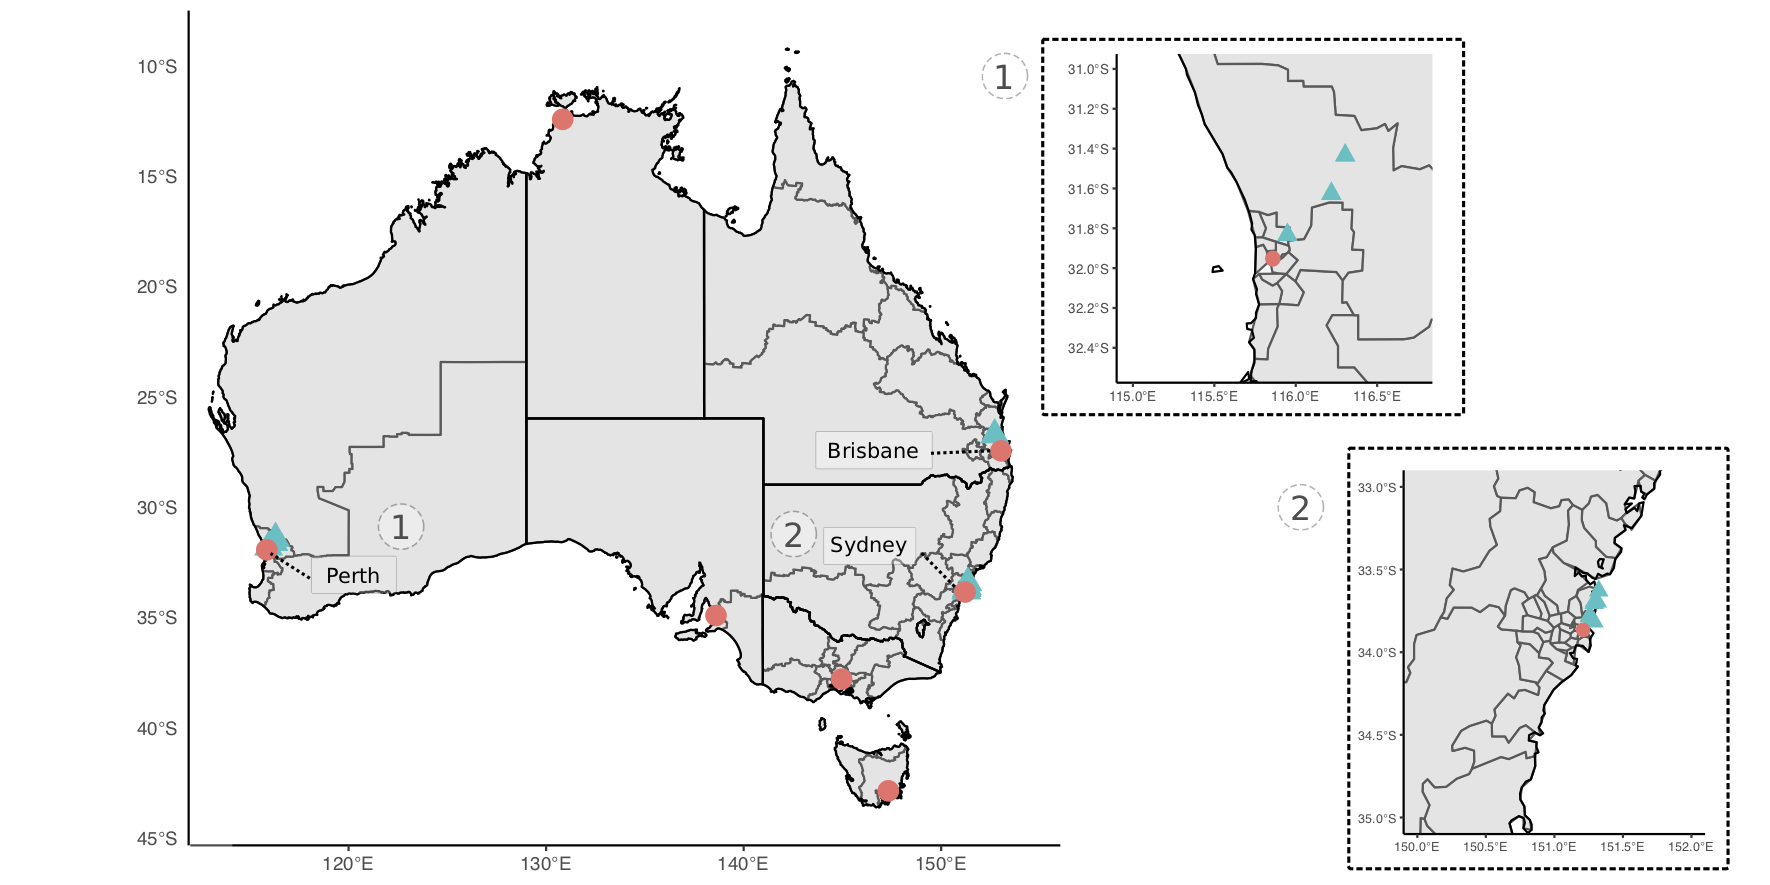
\includegraphics[width=0.95\linewidth]{figures/ms-figs/Ch4-map} \caption[Map of study sites for wildlife samples.]{Map of study sites for collection of wildlife sample used in haemoprotozoan surveillance (denoted by blue; capital cities denoted for reference). Insert maps of sites in (1) Perth, Western Australia and (2) Sydney, New South Wales.}\label{fig:Ch4map}
\end{figure}

\textbf{Haemoparasite microscopy}

Thin blood smears were made from whole blood, allowed to air dry and then fixed with 100\% methanol.
Slides were stained with Diff Quick (Siemens, Germany) and a coverslip was mounted using DPX neutral mounting medium (LabChem, Australia).
The smears were inspected by light microscopy (Olympus BX51) for the presence of haemoprotozoans at magnifications of ×400 and under oil immersion at ×1000.

\hypertarget{dna-extractions-1}{%
\subsection{DNA extractions}\label{dna-extractions-1}}

Total genomic DNA (gDNA) was extracted from 200 \(\mu\)L of blood using a MasterPure DNA purification kit (Epicentre\textregistered Biotechnologies, Madison, Wisconsin, U.S.A) following the manufacturer's recommendations.
Where 200 \(\mu\)L of blood was not available, sterile DNA free phosphate-buffered saline (PBS) was used to make samples up to 200 \(\mu\)L. Genomic DNA was eluted in 30--40 \(\mu\)L of TE buffer and stored at -20\(^\circ\)C until further processing.

Tissue samples (skin and spleen) were first rinsed in sterile, DNA-free PBS and cut into small pieces using a sterile scalpel blade. Samples were homogenised in 180 \(\mu\)L of buffer ATL and 20 \(\mu\)L of proteinase K was added prior to incubation at 56\(^\circ\)C for \textasciitilde{} 16 hours. gDNA was extracted using the QIAamp DNA Mini Kit (QIAGEN, Germany) following the manufacturer's protocols and final elution volume was decreased to 40--50 \(\mu\)L to optimise gDNA yield.

Once ticks were identified they were surface-sterilised by washing in 10 \% hypochlorite solution, rinsed in 70 \% ethanol and DNA-free PBS, and then air-dried.
Genomic DNA was extracted using the DNeasy Blood and Tissue kit (QIAGEN, Germany) for adults or the QIAamp DNA Mini Kit (QIAGEN, Germany) for nymphs and larvae.
Due to the large number of larvae collected from some animals and the expected low DNA yield, in some cases up to 5 larvae were pooled based on host, species and engorgement status.
Ticks were placed in a 2 mL safe lock Eppendorf tube with a 5 mm steel bead, frozen in liquid nitrogen for 1 min and homogenised by shaking at 40 Hz in a Tissue Lyser LT (QIAGEN, Germany).
Final elution of DNA was adjusted according to tick size, between 30-150 \(\mu\)L of AE buffer was added to the silicon membrane.

Extraction blank controls (EXBs) consisting of 200 \(\mu\)L sterile DNA free PBS, were included randomly in each extraction batch. Blood and tissue samples were extracted in a separate laboratory, away from where ticks were processed to avoid cross-contamination between sample types. Sterile procedures were followed throughout the laboratory process.

\hypertarget{trypanosomes}{%
\subsection{Trypanosomes}\label{trypanosomes}}

\textbf{Validation}

Positive controls of \emph{Leishmania infantum} (bone marrow sample obtained from a domestic dog), \emph{Leishmania macropodum} (culture isolate), \emph{Trypanosoma binneyi} (blood sample obtained from a platypus, \emph{Ornithorhynchus anatinus}), \emph{Trypanosoma cyclops}-like (blood sample obtained from a Tasmanian devil, \emph{Sarcophilus harrisii}) and \emph{Trypanosoma teixeirae} (blood sample obtained from a flying fox, \emph{Pteropus scapulatus}) were used for assay validation.

\textbf{Sequencing and bioinformatics}

A high-throughput metabarcoding approach was used to sequence samples (blood, ticks and tissue) using the Illumina MiSeq platform. Sample libraries were built following the 16S Metagenomic Sequencing Library Preparation (Illumina Part \# 15044223 Rev.~B), with amplicon PCR primers containing an Illumina MiSeq adapter sequences (Table \ref{tab:T4primers}).

Kinetoplastid libraries were built targeting the \emph{18S rRNA} hypervariable region v7-8. Samples were amplified using a semi-nested PCR with primary primers S825F and TryAllR1 \autocite{maslovPhylogenyTrypanosomesInferred1996,barbosaIncreasedGeneticDiversity2017} and the secondary primers S825F and 662R \autocite{maslovPhylogenyTrypanosomesInferred1996} containing MiSeq sequence adapters.
Reactions were carried out in 25 \(\mu\)L volumes each containing: 1X buffer (KAPA Biosystems, South Africa), 2.0 mM MgCl\textsubscript{2}, 0.4 mg/ml of bovine serum albumin (Fisher Biotech), 0.4 \(\mu\)M of each primer, 0.25 mM of each dNTP, 0.5 U of Taq (KAPA Biosystems, South Africa) and 2\(\mu\)L of gDNA or 1 \(\mu\)L of primary PCR product.
Thermal cycling conditions were as follows; 95\(^\circ\)C for 3 mins, followed by 40 cycles of 95\(^\circ\)C for 30 secs, 53\(^\circ\)C (primary) or 55\(^\circ\)C (secondary) for 30 secs, 72\(^\circ\)C for 30 secs; and a final extension step of 72\(^\circ\)C for 5 mins.

Amplicon PCR products were then indexed using the Nextera XT DNA library preparation kit in 25 \(\mu\)L volumes following the manufacturer's recommendations.
All PCRs included no template controls (NTC) during each reaction set up and PCRs were performed under strict laboratory conditions.
Amplicons were then dual-indexed using the Nextera XT index kit.
Reactions were performed in 25 \(\mu\)L volumes following the manufacturer's recommendations.
Libraries were purified with Axygen PCR clean up beads and quantified using Qubit High Sensitivity dsDNA assay kit (Thermo Fisher Scientific, Waltham, MA, USA).
Concentration of trypanosome libraries was highly variable among samples.
To ensure samples were analysed uniformly, all libraries were included for sequencing regardless of apparent negative result after PCR (as indicated by gel electrophoresis or Qubit concentration).
This decision was made to ensure that even low levels of haemoprotozoans would be detected.
Libraries were shipped to the Australian Genomic Research Facility (Melbourne, Australia) for final QC and sequenced on an Illumina MiSeq using v2 chemistry (2 x 250 paired-end).

Trypanosome MiSeq data was analysed using a bioinformatic pipeline with the program USEARCH v11 \autocite{edgarSearchClusteringOrders2010}.
Briefly paired-end reads were merged and sequences matching forward and reverse primers were retrieved (max number of mismatches = 2).
Sequences were then quality-filtered and singletons were removed.
The unoise3 \autocite{edgarUNOISE2ImprovedErrorcorrection2016} algorithm was used to perform denoising (error-correction) and generate zero-radius taxonomic units (zOTUs).



\begin{table}

\caption[Primers used for haemoprotozoa detection in samples from ticks and wildlife.]{\label{tab:T4primers}List of primers used for the amplification of haemoprotozoans from Australian wildlife samples. References \textbf{1.} Maslov et al. \autocite*{maslovPhylogenyTrypanosomesInferred1996}, \textbf{2.} Barbosa et al. \autocite*{barbosaIncreasedGeneticDiversity2017}, \textbf{3.} Jefferies et al. \autocite*{jefferiesPCRRFLPDetectionDifferentiation2007}.}
\centering
\fontsize{8.5}{10.5}\selectfont
\begin{tabular}[t]{lll}
\toprule
Primer & Sequence (5'-3') & Reference\\
\midrule
\textbf{Kinetoplastid 18S rRNA} & \textbf{} & \textbf{}\\
S825F & ACCGTTTCGGCTTTTGTTGG & 1\\
TryAllR1 & GACTGTAACCTCAAAGCTTTCGC & 2\\
662R & GACTACAATGGTCTCTAATC & 1\\
\textbf{Piroplasm 18S rRNA} & \textbf{} & \textbf{}\\
BTF1 & GGCTCATTACAACAGTTATAG & 3\\
BTF2 & CCCAAAGACTTTGATTTCTCTC & 3\\
BTR1 & CCGTGCTAATTGTAGGGCTAATAC & 3\\
BTR2 & GGACTACGACGGTATCTGATCG & 3\\
\bottomrule
\end{tabular}
\end{table}

\hypertarget{piroplasm-and-hepatozoon}{%
\subsection{\texorpdfstring{Piroplasm and \emph{Hepatozoon}}{Piroplasm and Hepatozoon}}\label{piroplasm-and-hepatozoon}}

Blood samples were screened for piroplasms using a nested PCR targeting an \textasciitilde{} 800 bp product of the 18S rRNA gene (Table \ref{tab:T4primers}) \autocite{jefferiesPCRRFLPDetectionDifferentiation2007}.
Amplicon PCRs were carried out in 25 \(\mu\)L reactions each containing: 1X buffer (KAPA Biosystems, South Africa), 2.5 mM MgCl\textsubscript{2}, 0.4 \(\mu\)M of each primer, 0.25 mM of each dNTP, 0.5 U of Taq (KAPA Biosystems, South Africa) and 2 \(\mu\)L of gDNA or 1 \(\mu\)L of primary product.
Thermal cycling conditions were as follows; 95\(^\circ\)C for 2 mins, 58\(^\circ\)C for 1 min, 72\(^\circ\)C for 2 mins, followed by 40 cycles of 95\(^\circ\)C for 30 secs, 58\(^\circ\)C (primary) or 62\(^\circ\)C (secondary) for 20 secs, 72\(^\circ\)C for 1 min (primary) or 45 secs (secondary); and a final extension step of 72\(^\circ\)C for 5 mins.

Amplicons were visualised on agarose gel and products of the expected size were excised with a sterile scalpel blade and purified \autocite{yangSpecificQuantitativeDetection2013}.
Sanger sequencing was performed at the Australian Genome Research Facility (Perth, Western Australia) on an Applied Biosystems 3730XL DNA Analyzer using BigDye\textsuperscript{TM} Terminator v3.1 Cycle Sequencing Kit.
Nucleotide sequences were inspected and quality-filtered using Geneious 10.2.6 (\url{https://www.geneious.com}).

\hypertarget{sequence-identification-and-phylogenetics}{%
\subsection{Sequence identification and phylogenetics}\label{sequence-identification-and-phylogenetics}}

Nucleotide sequences were subject to BLAST analysis (BLASTN 2.11.0+ \autocite{zhangGreedyAlgorithmAligning2000,morgulisDatabaseIndexingProduction2008}) against NCBI nucleotide collection (nt) database.
Taxonomic lineage for each top hit (based on e-value score) was retrieved from NCBI taxonomy database using TaxonKit \autocite{weissHostReproductiveCycle2021}.
Final taxonomy assignment was then refined to the lowest common ancestor based on BLAST results (percentage identity, e-value and query coverage) and sequence alignment method.
For trypanosome metabarcoding positive and negative controls were inspected, a read cut-off threshold was set with sequence values \textless150 removed.
Generated sequences were then aligned with reference sequences retrieved from GenBank \autocite{bensonGenBank2017} using MUSCLE \autocite{edgarMUSCLEMultipleSequence2004}.
Phylogenies were inferred using the maximum likelihood (ML) method.
The optimal evolutionary model was selected using ModelFinder \autocite{kalyaanamoorthyModelFinderFastModel2017} based on Bayesian information criterion.
Phylogenetic analysis was performed in IQ-TREE v1.6.11 \autocite{nguyenIQTREEFastEffective2015} and bootstrap support was calculated using the ultrafast (UFBoot2) method with 10,000 replicates \autocite{hoangUFBoot2ImprovingUltrafast2018}.
Genetic sequence similarity was calculated using the Kimura 2-Parameter method \autocite{tamuraEstimationNumberNucleotide1993}.

Scripts for data analysis are available at \url{https://github.com/siobhon-egan/wildlife-haemoprotozoa}.
Raw Illumina MiSeq data has been deposited in the European Nucleotide Archive under project accession number PRJEB46031 (sample accession numbers ERS6633767--ERS6634241) and nucleotide data has been deposited in GenBank nucleotide database under accession numbers MW664957--MW664997, and MW676261--MW676287.

\hypertarget{prevalence}{%
\subsection{Prevalence}\label{prevalence}}

Confidence intervals for haemoprotozoan prevalence were calculated based on positive identification from blood samples only.
This is due to the inherent difficulties in calculating prevalence based on blood-fed ticks \autocite{estrada-penaPitfallsTickTickBorne2021}.
Additionally, the focus of the present study was the identification of haemoprotozoa from a wildlife host perspective.
Confidence intervals (95\% CIs) were calculated based on the Jeffreys interval \autocite{brownIntervalEstimationBinomial2001}.

\hypertarget{results-1}{%
\section{Results}\label{results-1}}

\hypertarget{sample-information}{%
\subsection{Sample information}\label{sample-information}}

Blood samples were collected from 134 individuals: 70 black rats (\emph{Rattus rattus}), 18 common brush-tailed possums (\emph{Trichosurus vulpecula}), two bush rats (\emph{Rattus fuscipes}), 22 chuditch (\emph{Dasyurus geoffroii}), 20 long-nosed bandicoots (\emph{Perameles nasuta}), one quenda (\emph{Isoodon fusciventer}, previously \emph{Isoodon obesulus fusciventer}), and one swamp rat (\emph{Rattus lutreolus}).
A total of 52.2\% (95\% CI: 43.8--60.5\%) of animals were positive for at least one haemoprotozoan, with 19.4\% (95\% CI: 13.4--26.7\%) of animals positive for more than one species (Figure \ref{fig:Ch4upset}).

A total of 205 tick DNA pools which consisted of 257 ticks were extracted.
A total of six tick species were identified, the following numbers refer to DNA extracts analysed and total number of specimens for each species respectively: \emph{Amblyomma triguttatum} (4/5), \emph{Ixodes antechini} (1/1), \emph{Ixodes australiensis} (1/1), \emph{Ixodes holocyclus} (67/81), \emph{Ixodes tasmani} (90/103) and \emph{Ixodes trichosuri} (37/48). An additional 5 DNA pools which included 18 specimens were identified as a mix of \emph{Ix. holocyclus} and \emph{Ix. trichousri}.

\begin{figure}
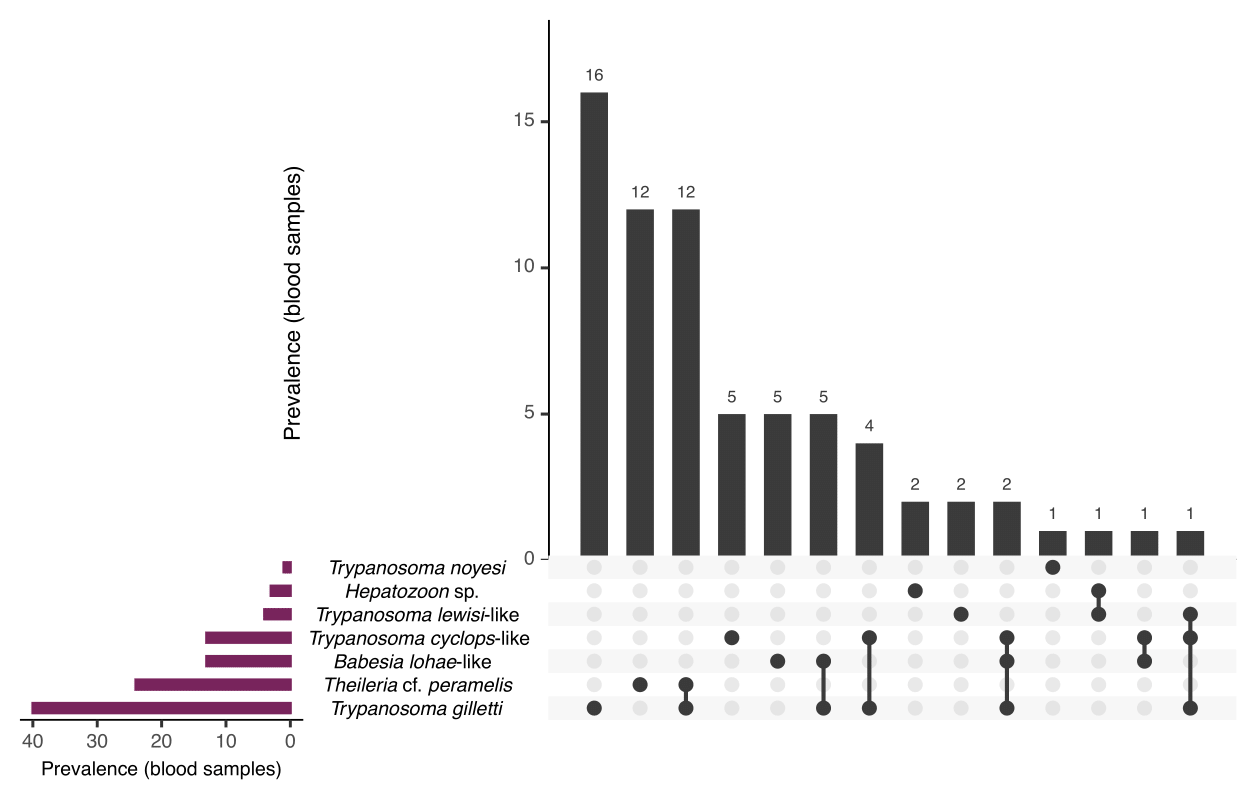
\includegraphics[width=0.95\linewidth]{figures/ms-figs/Ch4-haem-blood-prev} \caption[Summary of haemoprotozoa prevalence in wildlife blood samples.]{Prevalence of haemoprotozoans identified from wildlife blood samples presented as number infected of individuals. Data are visualised using UpSet plot showing set intersections of \textit{Trypanosoma}, \textit{Theileria}, \textit{Babesia} and \textit{Hepatozoon} species identified. Total number of individuals sampled: \textit{n} = 134.}\label{fig:Ch4upset}
\end{figure}

\hypertarget{trypanosomes-1}{%
\subsection{Trypanosomes}\label{trypanosomes-1}}

\textbf{Bioinformatic results}

A total of 51,719,606 raw sequences were obtained from Illumina MiSeq, with 24,138,102 sequences after merging, 22,716,805 sequences after matching primers and then 12,047,863 sequences post-quality filtering (representing \textasciitilde23.3\% of raw sequences).
After denoising, 10,283,530 sequences were obtained from samples; 1,355,654 sequences from positive controls and 305,910 negative controls (Figure \ref{fig:FA41}).
The average length of sequences post-filtering was 298 bp for positive controls (see validation) and 271 bp for samples.
Denoising via the unoise3 algorithm produced 1,630 zOTUs (avg length 233 bp). Taxonomic assignment showed 607 zOTUs were assigned to Eukaryota, with 346 zOTUs belonging to Kinetoplastea (Phylum: Euglenozoa) and 129 zOTUs identified as family Trypanosomatidae.
A final 65 Trypanosomatidae zOTUs remained after removing low abundant sequences (i.e.~\textless{} 150 sequences) with a total of 6,959,707 sequences (samples = 5,811,323; positive controls = 1,148,384) (see \protect\hyperlink{supplementary-table-e2.1}{Supplementary Table E2.1} for sequence data and taxonomy including BLAST results).
For phylogenetic reconstruction, a representative subset of 27 zOTUs were used (Figure \ref{fig:Ch4tryptree}); of which 22 zOTUs were from samples and an additional five zOTUs that were generated from positive control samples.

\textbf{Validation}

All positive controls of \emph{L. infantum}, \emph{L. macropodum}, \emph{Tr. binneyi}, \emph{Tr. cyclops}-like and \emph{Tr. teixeirae} were successfully amplified, confirming the ability of this assay to detect a phylogenetically diverse range of trypanosome sequences (\protect\hyperlink{supplementary-table-e2.1}{Supplementary Table E2.1}). The resulting zOTUs were included in phylogenetic reconstruction (Figure \ref{fig:Ch4tryptree}).

\textbf{Samples}

Amplicon sequencing results from blood samples showed that 51 animals were positive for at least one species of \emph{Trypanosoma}.
Mixed trypanosome infections were identified in 5.2\% (95\% CI: 2.4--10.0\%) of blood samples from 4.3\% (95\% CI: 1.2--11.0\%) of black rats, 16.7\% (95\% CI: 4.9--38.1\%) of brush-tailed possums, and a single chuditch (4.6\%, 95\% CI: 0.5--19.3\%).
One black rat (1.4\%, 95\% CI: 0.2--6.9\%) was infected with three species of \emph{Trypanosoma}.

\emph{Trypanosoma gilletti} was the most abundant trypanosome species identified.
A total number of 69 zOTUs had a top match to \emph{Tr. gilletti}, eleven zOTUs had greater than 1000 reads, of which seven zOTUs were used for phylogenetic purposes in Figure \ref{fig:Ch4tryptree}.
This was the only species of \emph{Trypanosoma} identified in all three sample types (blood, ticks and tissue).
A total of 103 samples were positive (43 blood samples, 23 tick samples and 37 tissue samples); these samples were identified from 65 individuals.
Hosts identified as positive in blood and/or tissue samples for \emph{Tr. gilletti} were black rats (\emph{n} = 14), brush-tailed possums (\emph{n} = 12), chuditch (\emph{n} = 7) and long-nosed bandicoots (\emph{n} = 28).
Ticks positive for \emph{Tr. gilletti} were \emph{Ix. holocyclus} (larvae, nymphs and females), \emph{Ix. tasmani} (females) and \emph{Ix. trichosuri} (nymphs and females).
A thin trypomastigote stage was identified in the blood film of a long-nosed bandicoot (LNB113) (Figure \ref{fig:microscopy}A).
Amplicon metabarcoding of duplicate blood DNA extracts from this individual showed a single infection with \emph{Tr. gilletti}.

Fourteen zOTUs were most similar to members of the \emph{Trypanosoma cyclops} clade, matching sequences from Australian marsupials and leeches (GenBank: AJ620571, AJ620574, MT898517 and MT898518; 97.5--99.7\% similarity).
Representatives of the 12 most abundant zOTUs were used for the phylogenetic tree in Figure \ref{fig:Ch4tryptree}.
\emph{Trypanosoma cyclops}-like sequences were identified in 13 blood samples from 13 individuals (7 black rats, 5 brush-tailed possums and 1 chuditch were positive).
Only one tissue sample, from a brush-tailed possum (blood sample negative), was positive and all ticks were negative for \emph{Tr. cyclops}-like sequences.
Unfortunately, morphological verification of this trypanosome was difficult.
A potential amastigote stage of \emph{Tr. cyclops} was identified in a black rat (BR022) (Figure \ref{fig:microscopy}B) and a trypomastigote like stage from a second black rat (BR025) (Figure \ref{fig:microscopy}C), amplicon metabarcoding of both these animals identified a single trypanosome infection with \emph{Tr. cyclops}.

One sequence (zOTU 5) was identical to \emph{Trypanosoma} sp. BR042 (MN512227, 100\% similarity), which was characterised in Egan et al. \autocite*{eganMolecularIdentificationTrypanosoma2020} to explore the phylogeny of this \emph{Tr. lewisi}-like sequence.
This genotype was identified in three black rats and a single bush rat from two sites, North Head and Manly Dam in New South Wales.
Two black rats (sample IDs BR042 and BRAH1) were positive for \emph{Tr. lewisi}-like sequences in both tissue and blood samples.
No tick samples were positive for \emph{Tr. lewisi}-like sequences.
\emph{Trypanosoma noyesi} was identified in a single brush-tailed possum blood sample from Western Australia.
\emph{Trypanosoma vegrandis} (zOTU 47; GenBank: KC753534, 100\% similarity) was identified in an \emph{Am. triguttatum} (nymph) (ex quenda) from Western Australia.

\begin{figure}
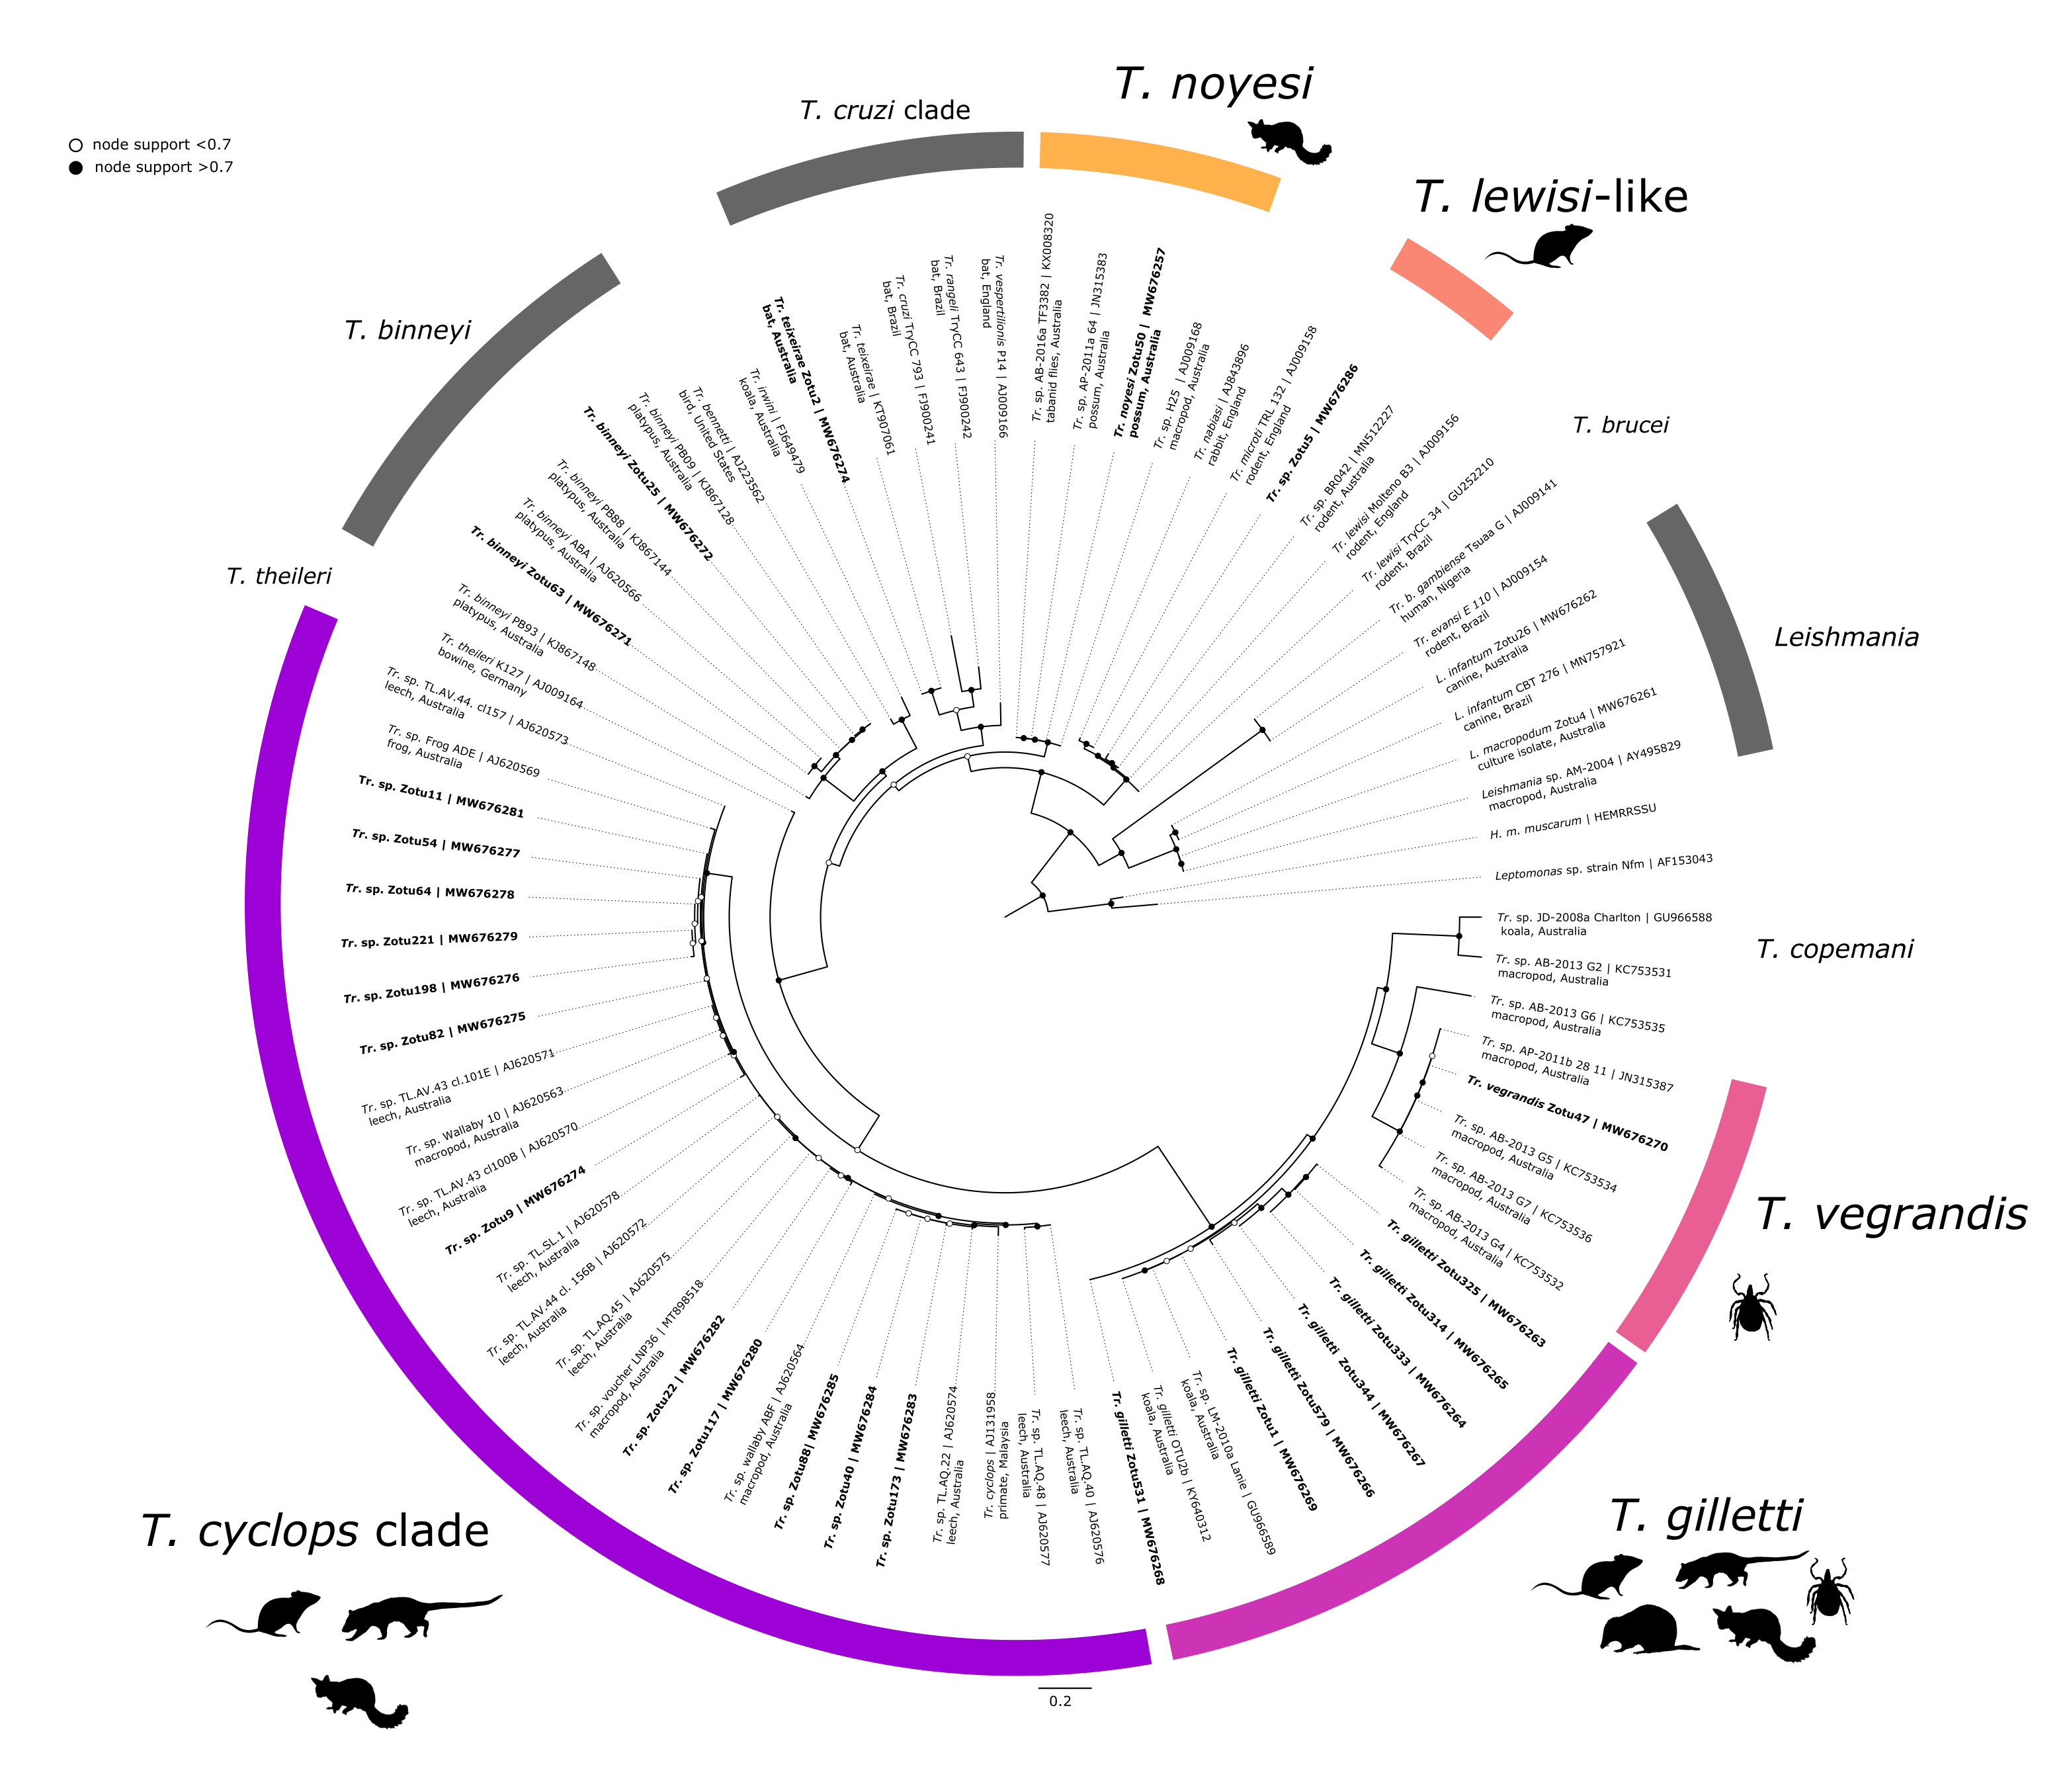
\includegraphics[width=0.95\linewidth]{figures/ms-figs/Ch4-trypNGStree} \caption[Phylogeny of trypanosomes species from wildlife.]{Maximum likelihood (ML) phylogenetic reconstruction of trypanosome zOTUs based on a 426 bp alignment of the 18S rRNA locus. Substitution model TIM3e + I + G4 with 10,000 replicates. Node values correspond to bootstrap support where values > 0.7 are indicated by filled circles. Number of substitutions per nucleotide position is represented by the scale-bar. Sequences generated in the present study are in bold.}\label{fig:Ch4tryptree}
\end{figure}

\begin{figure}
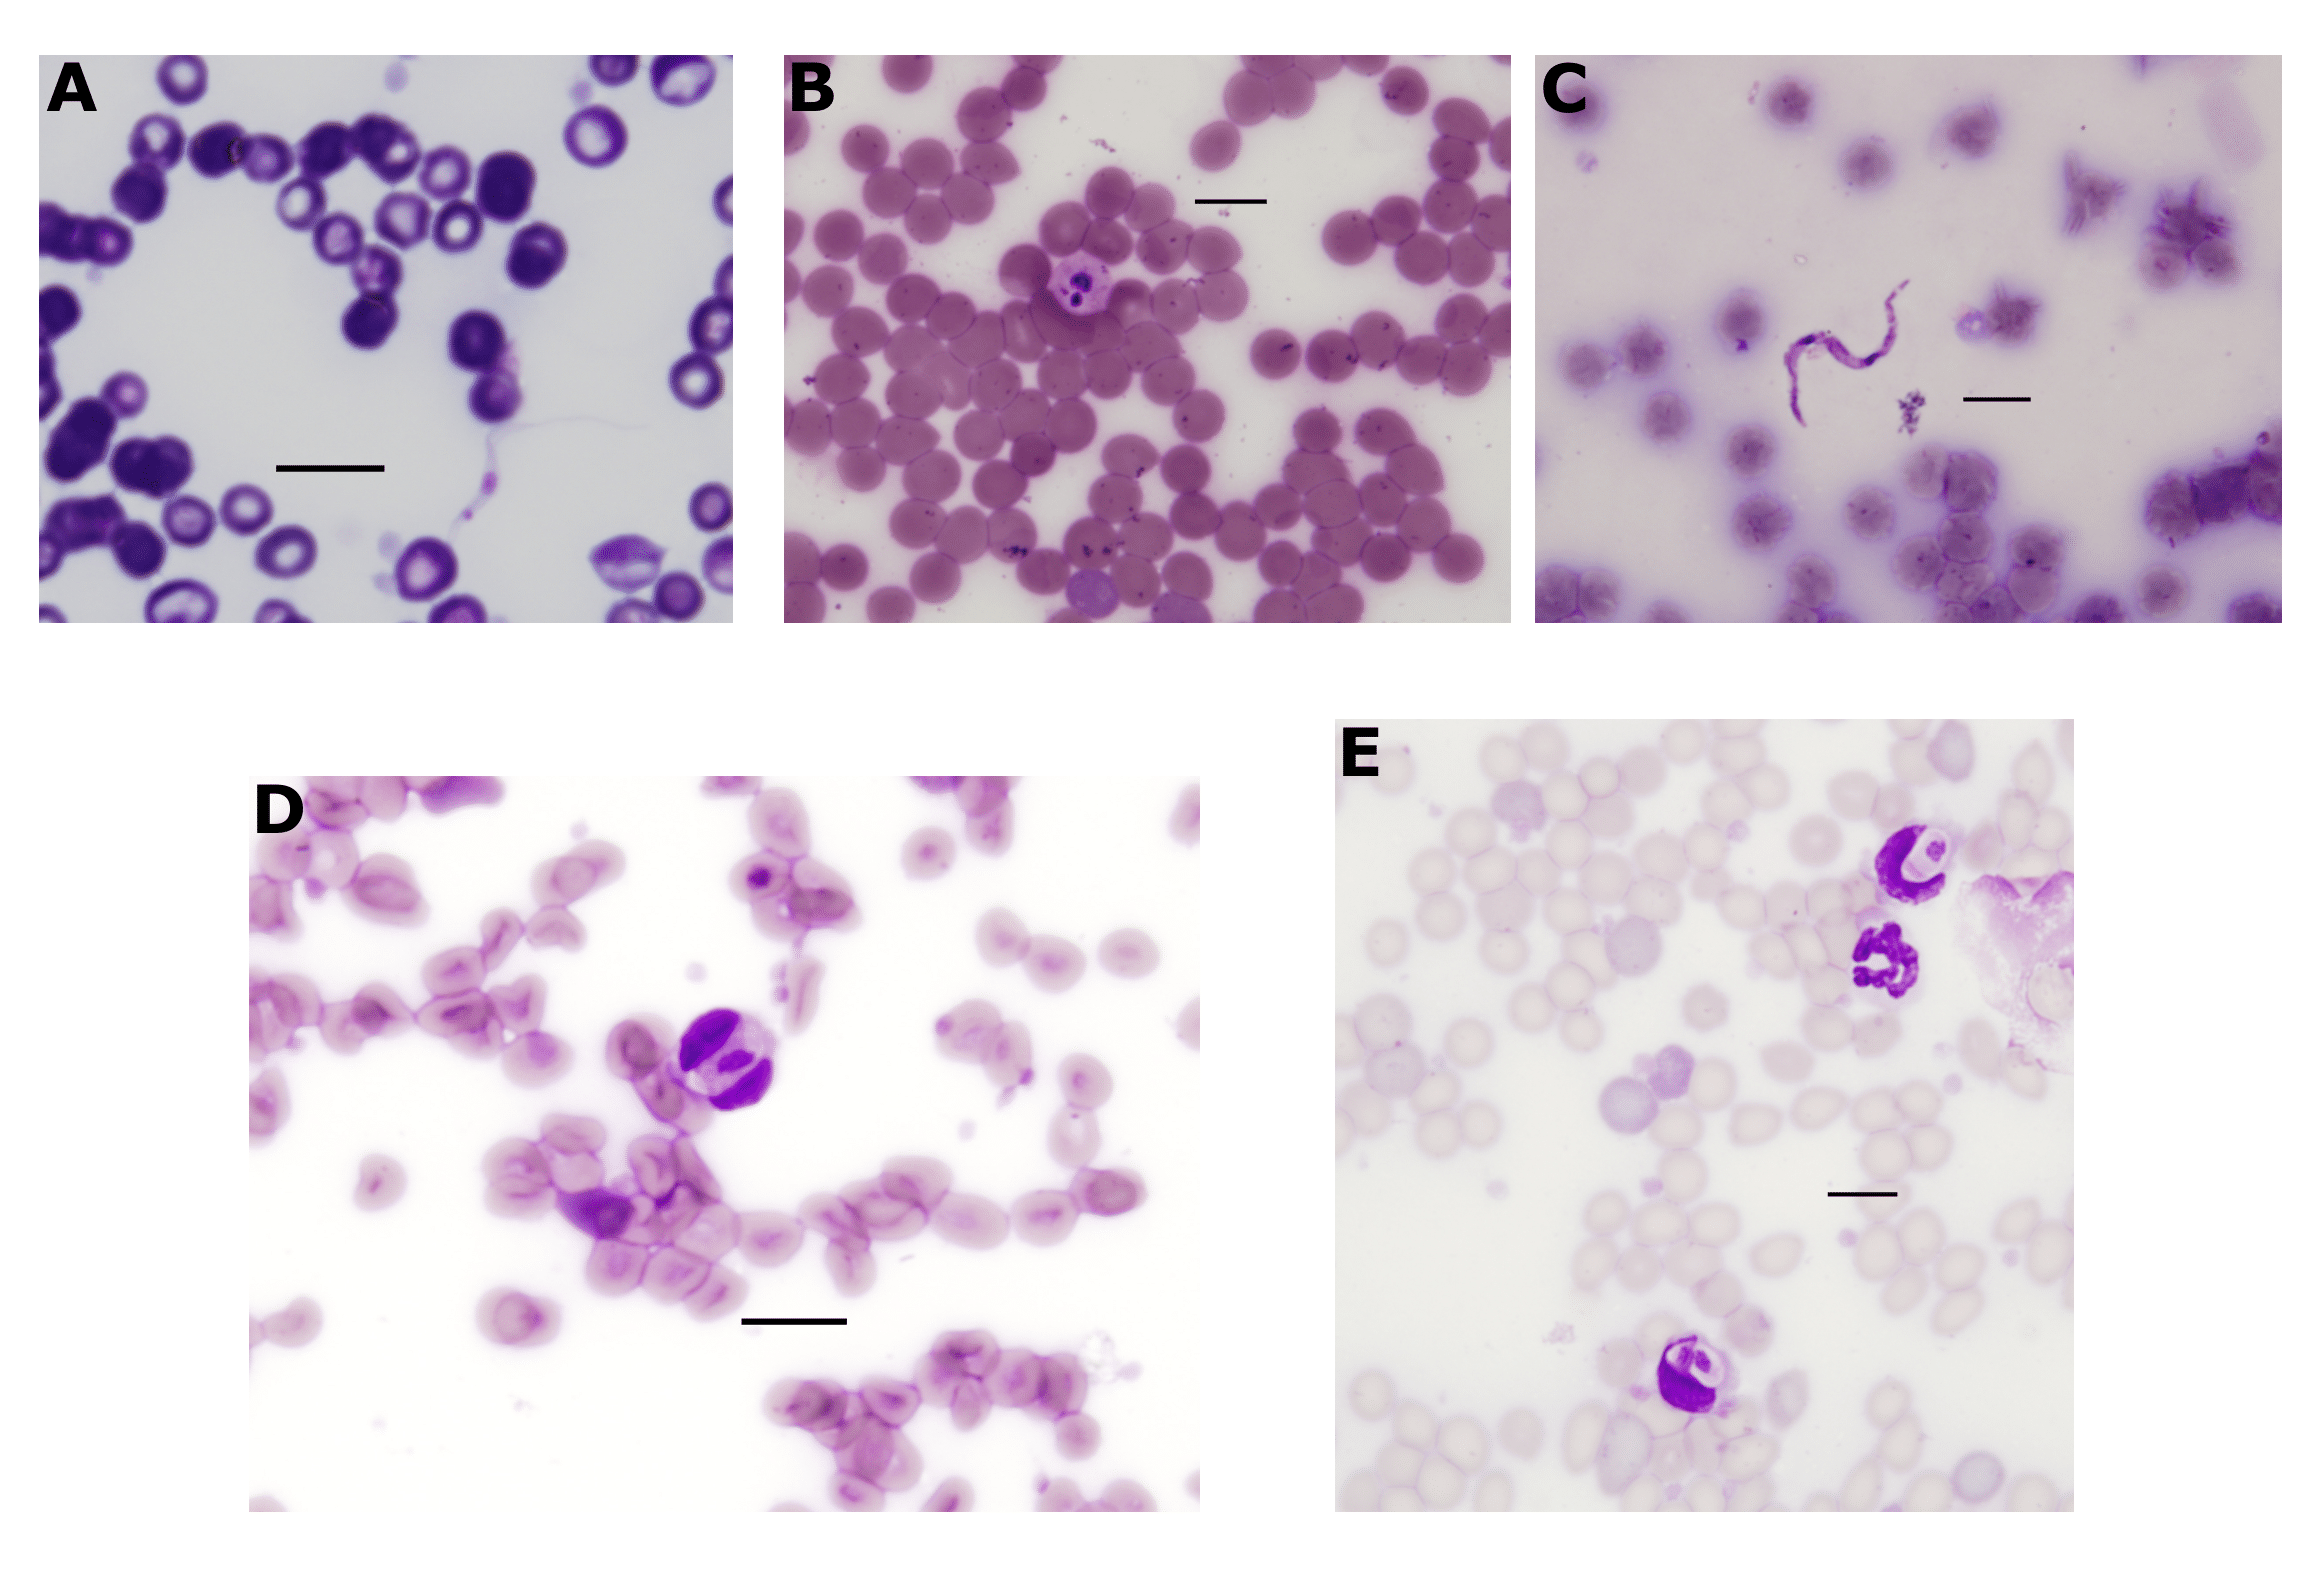
\includegraphics[width=0.95\linewidth]{figures/ms-figs/Ch4-microscopy-images} \caption[Haemoprotozoans identified in wildlife blood films.]{Haemoprotozoa identified in wildlife blood films. (A) Trypomastigote of \textit{Trypanosoma gilletti} from long-nosed bandicoot (LNB113). (B) Suspected amastigote of \textit{Trypanosoma cyclops} from black rat (BR022). (C) Trypomastigote of \textit{Trypanosoma cyclops} from black rat (BR025). (D-E) \textit{Hepatozoon} gametocytes within leukocytes of a black rat (BR039). All scale-bars: 10 $\mu M$.}\label{fig:microscopy}
\end{figure}

\hypertarget{piroplasms}{%
\subsection{Piroplasms}\label{piroplasms}}

\emph{Theileria} was identified in blood samples from 12.9\% (95\% CI: 6.6--22.2\%) of black rats and 75.0\% (95\% CI: 53.6--89.8\%) of long-nosed bandicoots from New South Wales.
All the sequences were 100\% identical to each other, and therefore one representative was used for phylogenetic analysis (Figure \ref{fig:F4pirotree}).
Sequences in the present study were identical to \emph{Theileria} sp. B16 and B60 (GenBank: MG251437 and MG251439) from \emph{Ix. tasmani} ticks ex. eastern barred bandicoot (\emph{Perameles gunnii}, Tasmania) and long-nosed bandicoot (Queensland), respectively.
The most similar named species was \emph{Theileria penicillata} (GenBank: EF554395; 97.4\%) from the long-nosed potoroo (\emph{Potorous tridactylus}) \autocite{leeTheileriaGilbertiSp2009}.
Phylogenetic reconstruction showed that the sequences in the present study formed a unique clade with those by Loh et al. \autocite*{lohMolecularSurveillancePiroplasms2018} (Figure \ref{fig:F4pirotree}) and demonstrated a divergence of 2.6\% to the nearest named species (see genetic distances in \protect\hyperlink{supplementary-table-e2.2}{Supplementary Table E2.2}).

All \emph{Babesia} sequences were obtained from 72.2\% (95\% CI: 49.4--88.5\%) of brush-tailed possum blood samples in New South Wales. Three genotypes were identified with 99.7--99.9\% similarity to each other (Figure \ref{fig:F4pirotree}).
The most similar sequence to those obtained in the present study was \emph{Babesia} sp. BP1 obtained from \emph{Ix. tasmani} (GenBank: MG251435, 99.7--100\% similar) ex. brush-tailed possum (NSW) \autocite{lohMolecularSurveillancePiroplasms2018}.
The next most similar was \emph{Babesia lohae} sequences identified from \emph{Ix. tasmani} ex brush-tailed possum (GenBank: MG251436, 98.3--98.6\% similar) \autocite{lohMolecularSurveillancePiroplasms2018} and \emph{Ix. holocyclus} ex. domestic cat (GenBank: MG593272, 98.2--98.5\% similar) \autocite{greayEndemicExoticNovel2018} (see genetic distances in \protect\hyperlink{supplementary-table-e2.2}{Supplementary Table E2.2}).

\begin{figure}
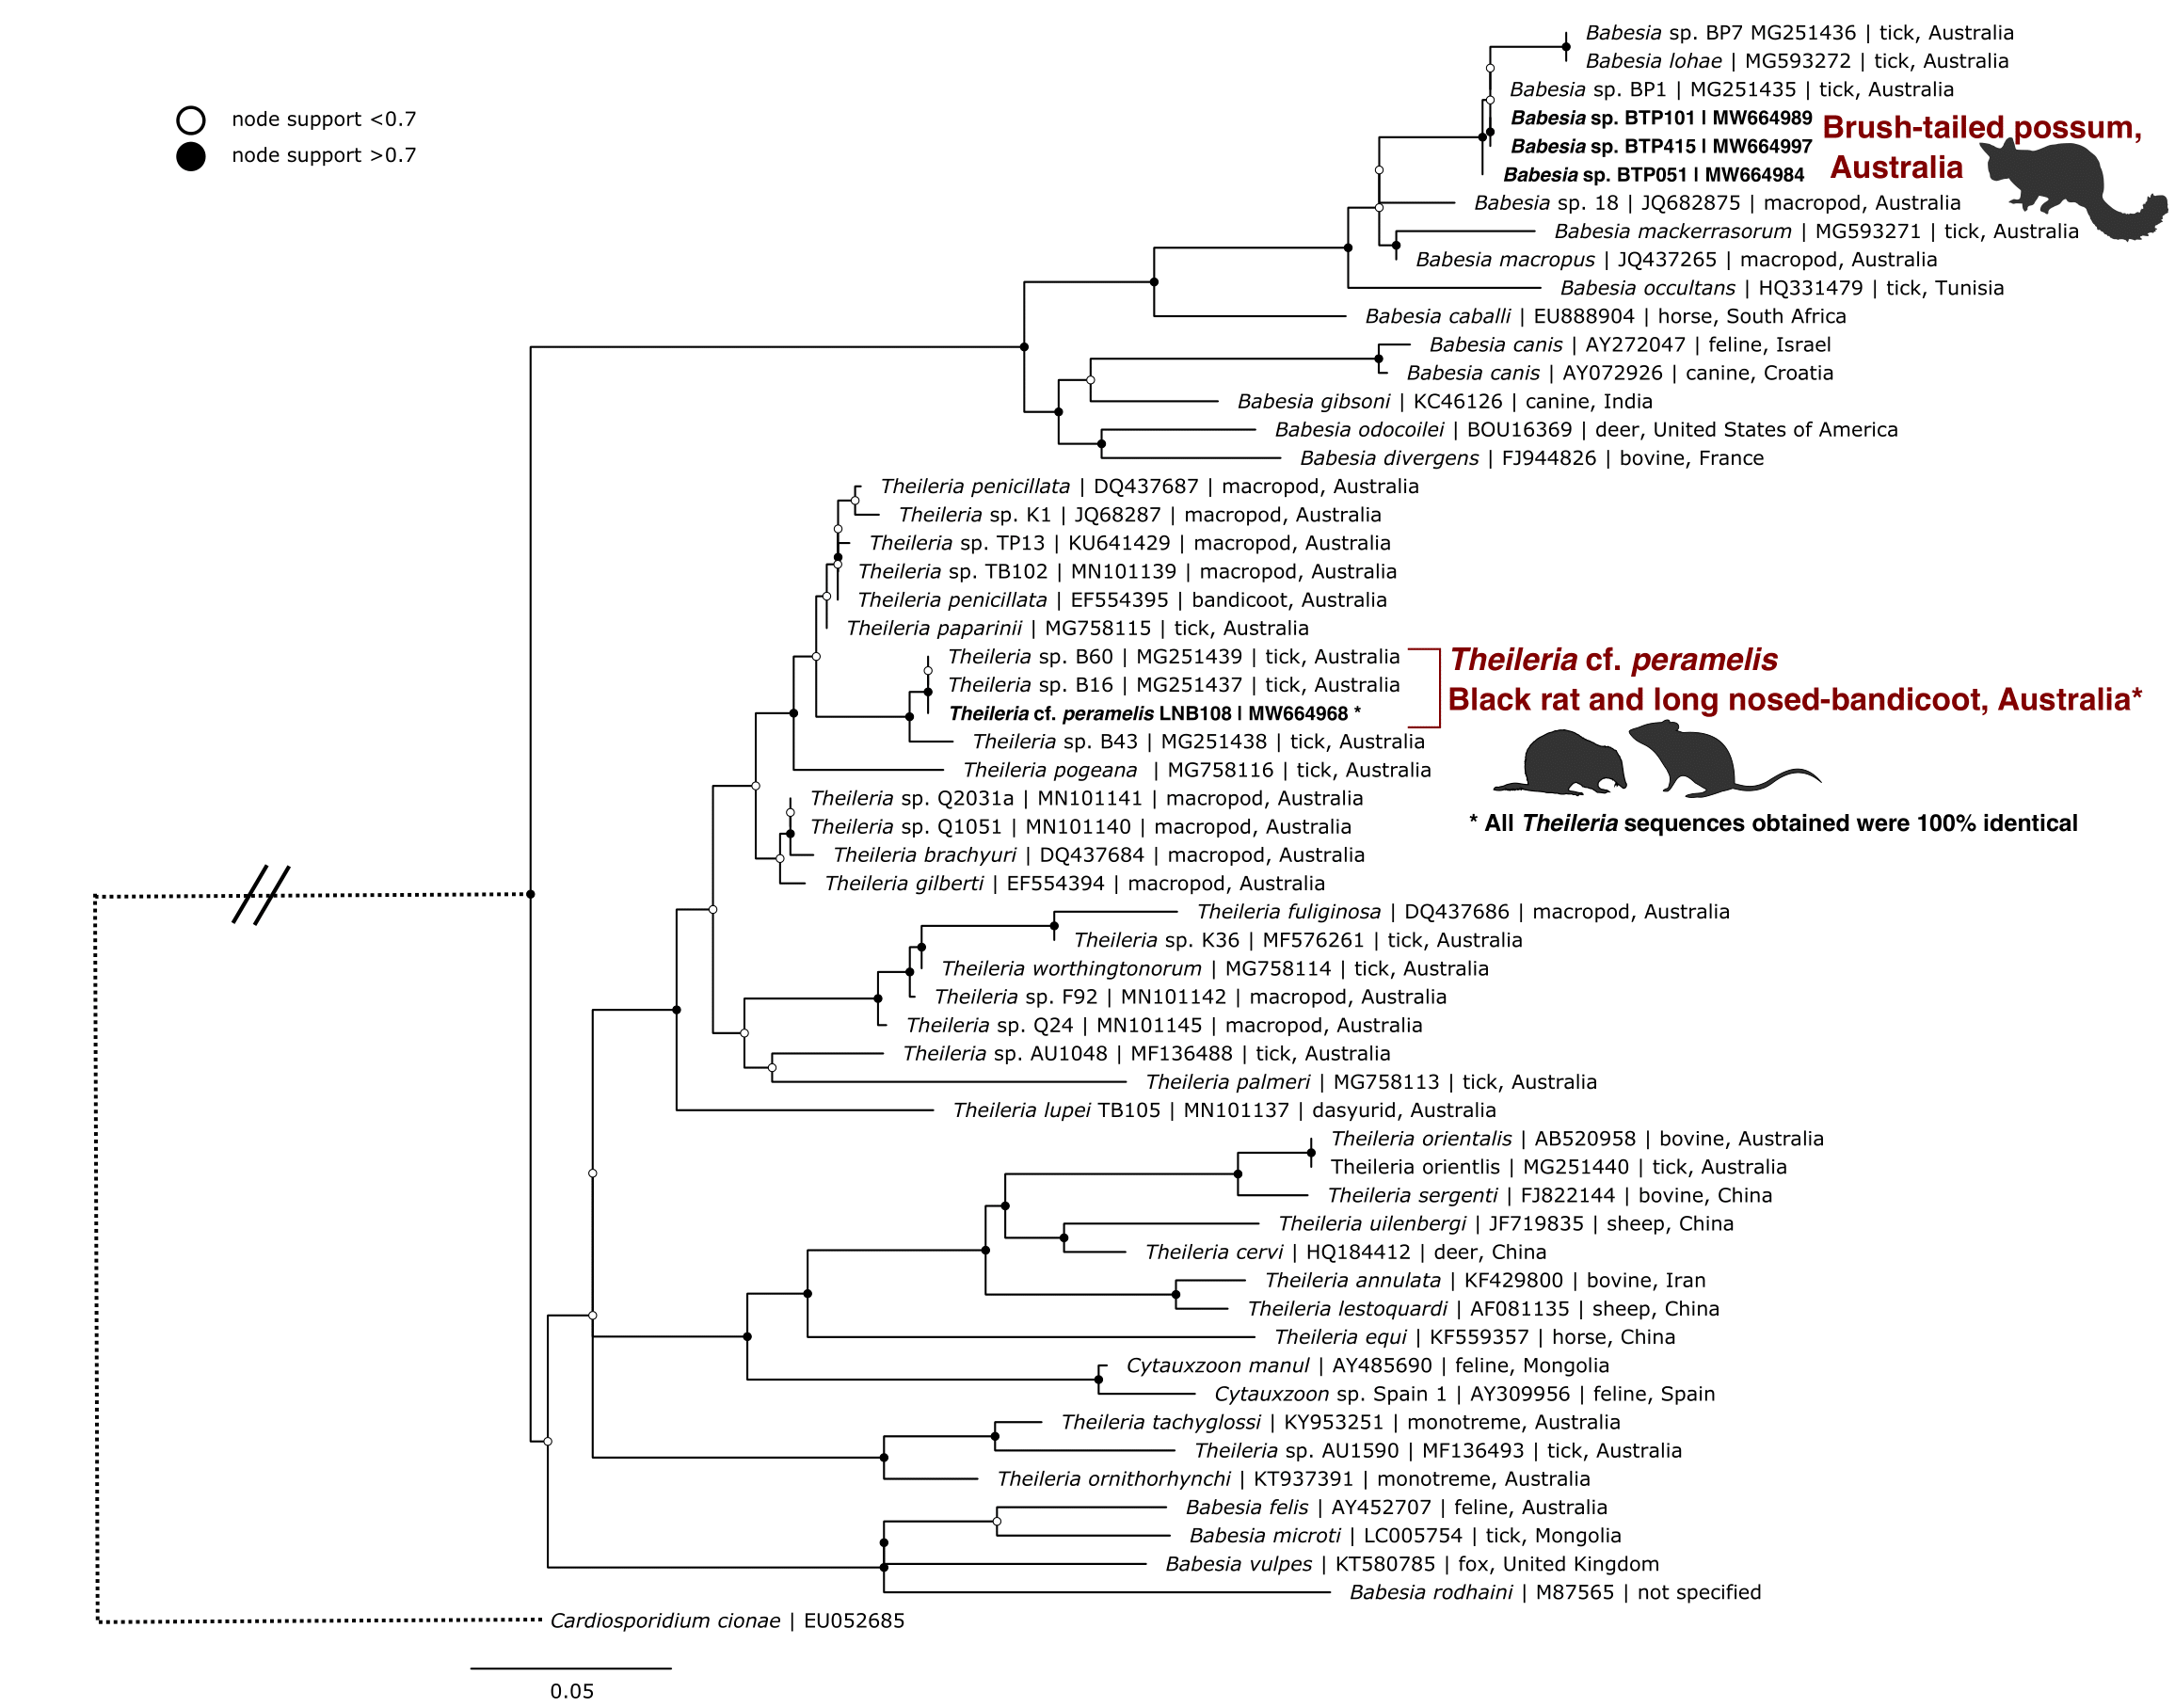
\includegraphics[width=0.95\linewidth]{figures/ms-figs/Ch4-pirotree} \caption[Phylogeny of piroplasm species.]{Maximum likelihood (ML) phylogenetic reconstruction of piroplasm species based on an 852 bp alignment of the 18S rRNA locus. Substitution model TIM3 + F + I + G4 with 10,000 replicates. Node values correspond to bootstrap support where values > 0.7 are indicated by filled circles. Number of substitutions per nucleotide position is represented by the scale-bar. Sequences generated in the present study are in bold.}\label{fig:F4pirotree}
\end{figure}

\hypertarget{hepatozoon}{%
\subsection{Hepatozoon}\label{hepatozoon}}

\emph{Hepatozoon} sequences were identified in three blood samples, two from bush rats and one from a black rat.
The two sequences from bush rats were 100\% identical to each other and the single sequence from a black rat was 98.8\% similar to the bush rat genotype (Figure \ref{fig:F4hepattree}).
The black rat genotype was most similar to \emph{Hepatozoon} sp. HepBiCM001 (GenBank: AB181504, 99.0\% similar) from a greater bandicoot rat (\emph{Bandicota indica}) in Thailand (Dantrakool et al.~unpublished), the next most similar were sequences from the bush rat, followed by \emph{Hepatozoon ayorgbor} (GenBank: EF157822, 98.63\% similar) from a ball python (\emph{Python regius}) in Ghana \autocite{slobodaNEWSPECIESHEPATOZOON2007} (see genetic distances in \protect\hyperlink{supplementary-table-e2.3}{Supplementary Table E2.3}).
The bush rat genotype was most similar to sequences from olive grass mice (\emph{Abrothrix olivaceus}) in Chile \autocite{merinoMolecularCharacterizationAncient2009}, genotypes \emph{Hepatozoon} sp. AO5 and A06 (GenBank: FJ719818 and FJ719817; both 98.8\% similar).
The next most similar sequence to the bush rat genotype was \emph{Hepatozoon ophisauri} (host unknown) from Iran (Zechmeisterova, unpublished) (GenBank: MN723845, 98.8\% similar).
Microscopy of blood films from positive individuals identified oval shaped \emph{Hepatozoon} gametocytes within leukocytes (Figure \ref{fig:microscopy}D-E).

\begin{figure}
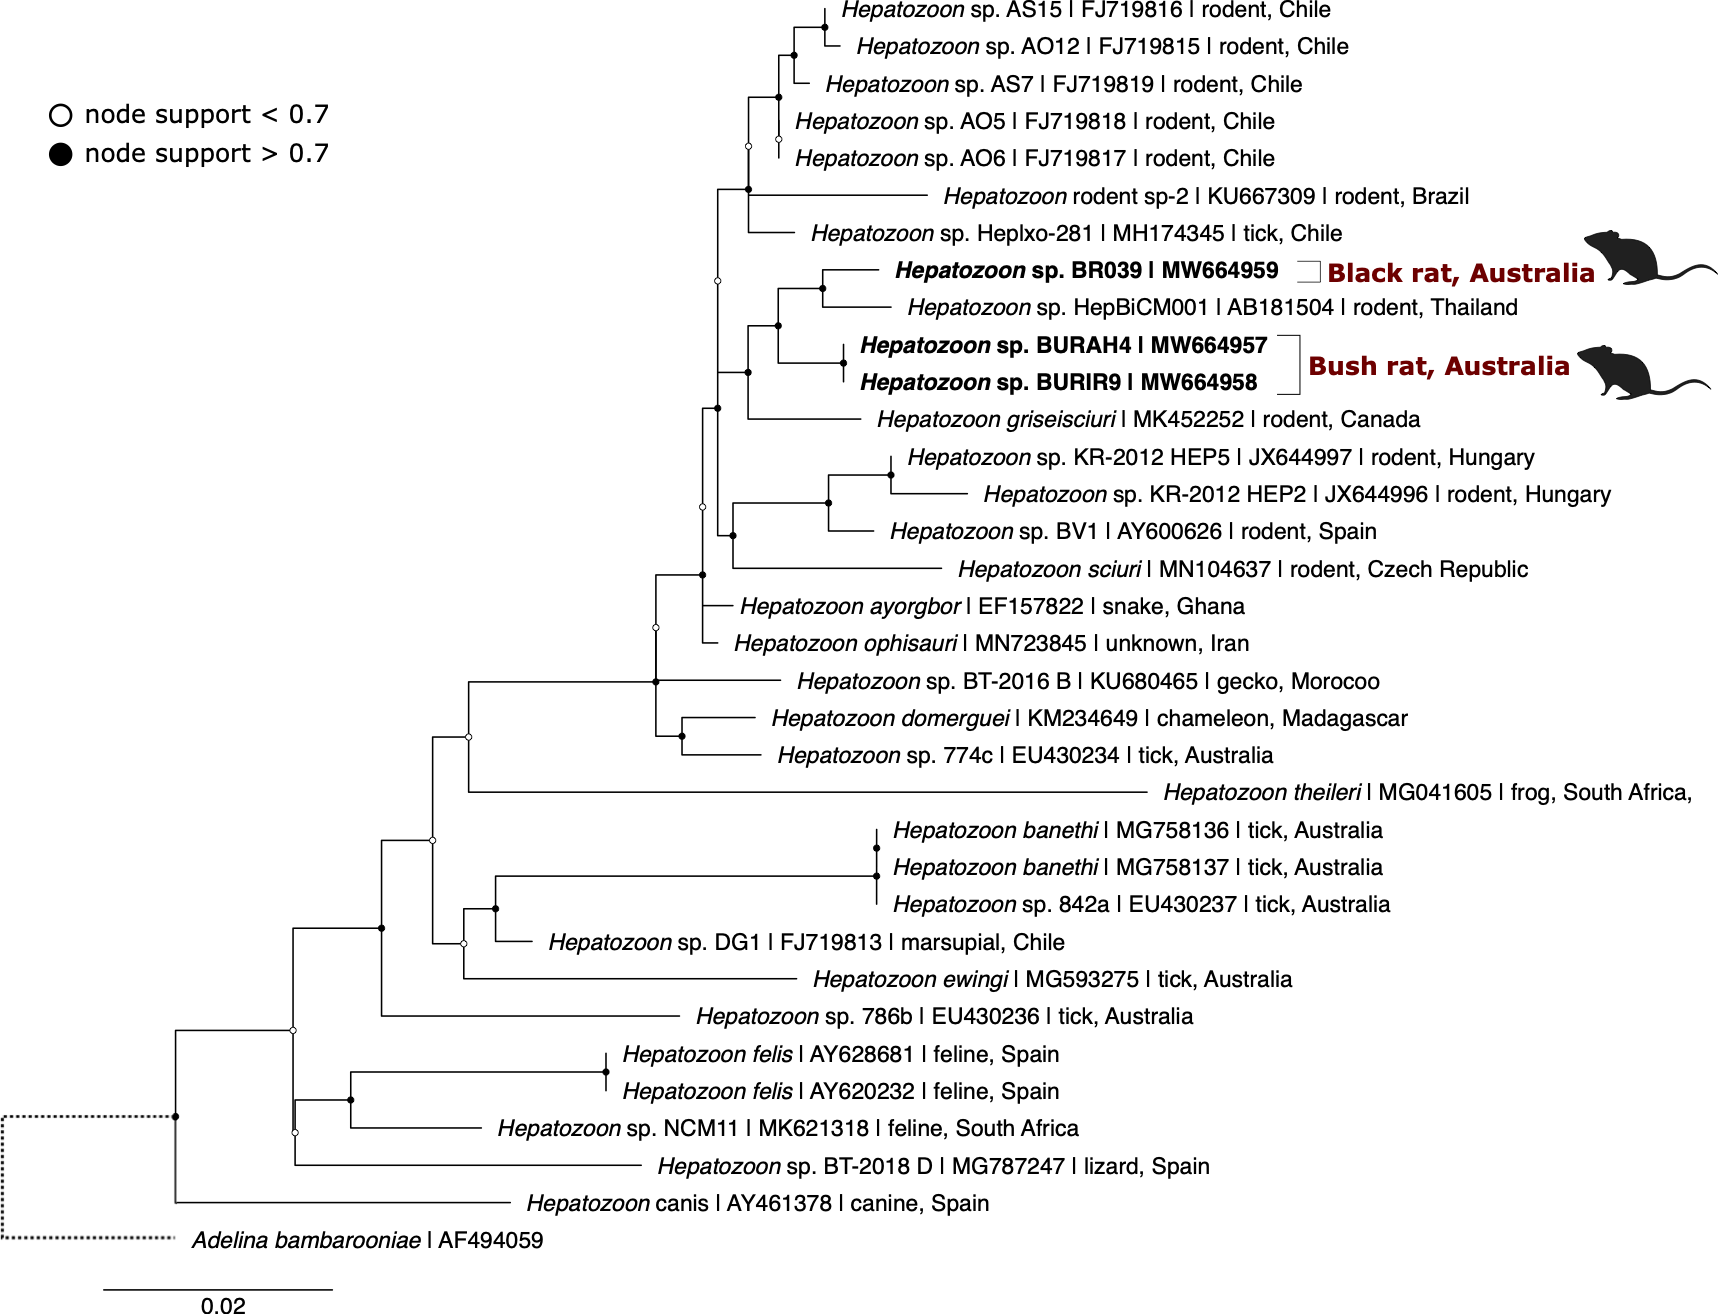
\includegraphics[width=0.95\linewidth]{figures/ms-figs/Ch4-hepattree} \caption[Phylogeny of \textit{Hepatozoon} species.]{Maximum likelihood (ML) phylogenetic reconstruction of \textit{Hepatozoon} based on an 829 bp alignment of the 18S rRNA locus. Substitution model HKY + F + I + G4 with 10,000 replicates. Node values correspond to bootstrap support where values > 0.7 are indicated by filled circles. Number of substitutions per nucleotide position is represented by the scale-bar. Sequences generated in the present study are in bold.}\label{fig:F4hepattree}
\end{figure}

\hypertarget{discussion-1}{%
\section{Discussion}\label{discussion-1}}

This study identified a total of eight species of haemoprotozoans from Australian wildlife; seven species were identified from hosts directly (blood and tissue samples), and an additional species, \emph{Tr. vegrandis}, was identified from a single tick (\emph{Am. triguttatum}). Black rats had the highest diversity with five haemoprotozoan species.

To the best of the authors' knowledge this is the first report of \emph{Tr. cyclops}-like genotypes from black rats, brush-tailed possums, and a chuditch.
In addition, \emph{Tr. gilletti} from black rats, brush-tailed possums, chuditch and long-nosed bandicoots were also identified in these hosts for the first time. This is the first identification of \emph{Babesia} from brush-tailed possums. We also report the first molecular sequences obtained from presumed \emph{Theileria} cf.~\emph{peramelis} and a new host record of this species from black rats. A putative novel \emph{Hepatozoon} species was identified from black rats and bush rats.

\hypertarget{trypanosomes-2}{%
\subsection{Trypanosomes}\label{trypanosomes-2}}

\textbf{Validation}

To identify trypanosome infection a previously developed high-throughput assay was used. This assay was previously used to identify \emph{Trypanosoma} from koala (\emph{Phascolarctos cinereus}) blood samples and ticks \autocite{barbosaIncreasedGeneticDiversity2017} and has been since used to identify co-infections in woylie (brush-tailed bettong, \emph{Bettongia penicillata}) blood samples \autocite{cooperNextGenerationSequencing2018}.
In the present study, the assay was validated on additional controls using the phylogenetically distinct \emph{Tr. binneyi} \autocite{papariniNovelGenotypesTrypanosoma2014}, and members from the genus \emph{Leishmania} including \emph{L. macropodum} and \emph{L. infantum}.
Validation of the assay on additional \emph{Leishmania} species indicates that the absence of \emph{Leishmania} in the present study most likely reflects a true negative finding.

\textbf{Amplification of non-target sequences}

The low rate of sequences retained after bioinformatic analysis in the present study is likely due to the co-amplification of non-target sequences.
In order to ensure final sequences generated are representative of true biological sequences it is important that amplicons undergo best practice bioinformatic analysis.
The level of sequences retained in the present study (\textasciitilde23.3\%) were similar to that reported from Huggins et al. \autocite*{hugginsNovelMetabarcodingDiagnostic2019} (17.0\%).
However, more widespread comparisons are difficult to make as in many cases sequences retained throughout bioinformatics are not adequately reported \autocite{squarreDiversityTrypanosomesWildlife2020,wahabNovelMetabarcoded18S2020}.
Due to the nature of the Illumina sequencing platform, artificial sequences or chimeras can be generated, particularly when libraries are prepared by PCR amplification methods.
Steps taken to avoid the impact of this included using primers without degenerate bases, including a G/C clamp at the 3' end of primers, use of high fidelity Taq polymerases and minimising the number of PCR cycles \autocite{bradleyDesignEvaluationIllumina2016}.
The issue of abundance comparisons in amplicon sequencing has still not been well resolved. While attempts are beginning to improve in the case of bacterial 16S amplicon studies, there is still much work to be done for 18S amplicon studies.
Differences in amplification efficiencies among targets and gene copy number variations are two of the main factors impacting sequence abundance measures in amplicon sequencing \autocite{bradleyDesignEvaluationIllumina2016}.
Therefore, comparisons of sequence numbers as a measure for trypanosome abundance were not made in the present study.

\textbf{\emph{Trypanosoma} sp. identified}

\emph{Trypanosoma gilletti} was first described from koalas in Queensland and New South Wales \autocite{mcinnesNovelTrypanosomeTrypanosoma2011}.
At the time of description, morphological characterisation was not possible as trypomastigotes were only identified in blood smears from one koala that was co-infected with \emph{Tr. copemani}.
Since its description there have been four additional reports of \emph{Tr. gilletti}; (i) further reports in koalas and their ticks (\emph{Ix. holocyclus} and \emph{Ix. tasmani}) \autocite{barbosaIncreasedGeneticDiversity2017}; (ii) woylies from Western Australia {[}\textcite{cooperNextGenerationSequencing2018};\textcite{northoverIncreasedTrypanosomaSpp2019};{]}; (iii) swamp wallaby (\emph{Wallabia bicolor}) and southern brown bandicoot (\emph{Isoodon obesulus}) in New South Wales \autocite{ortiz-baezMetatranscriptomicIdentificationTrypanosoma2020}; and (iv) long-nosed potoroos from New South Wales \autocite{hallBaselineHealthParameters2021}.
Therefore, the present study reports the first host records of \emph{Tr. gilletti} from black rats, brush-tailed possum, chuditch and long-nosed bandicoots and the first identification in \emph{Ix. trichosuri}.
Despite its high prevalence from amplicon sequencing, \emph{Tr. gilletti} was not readily detected in corresponding blood films from positive animals.
A slender trypomastigote was identified in one long-nosed bandicoot with a single infection of \emph{Tr. gilletti}.
This slender form had a large central nucleus, with the kinetoplast located at the posterior end of the body and is consistent with findings of McInnes \autocite*{mcinnesNovelTrypanosomeTrypanosoma2011}.

Until recently, records of the \emph{Tr. cyclops} clade were sparse. Since 2020 however, there have been at least four reports of this clade.
\emph{Trypanosoma cyclops} genotypes have been identified from Tasmanian devil blood samples (Tasmania, Australia) \autocite{eganBloodParasitesEndangered2020}, rodent liver samples (\emph{Bunomys}, \emph{Maxomys}, \emph{Paucidentomys} and \emph{Rattus}) (Indonesia) \autocite{winterhoffNativeIntroducedTrypanosome2020}, swamp wallaby cranial tissue (New South Wales, Australia) \autocite{ortiz-baezMetatranscriptomicIdentificationTrypanosoma2020} and long-nosed potoroo blood samples (New South Wales, Australia) \autocite{hallBaselineHealthParameters2021}.
The results presented here provide further support for the widespread distribution of this trypanosome with regards to geographical location and hosts.
The evidence therefore indicates that the \emph{Tr. cyclops} clade is endemic to the Asia-Pacific regions including Australia.
Trypanosome-like stages were detected in blood smears of two black rats.
The round circular stage was consistent with an amastigote form given the presence of both a kinetoplast and nuclear region and the absence of a free flagellum.
The trypomastigote-like stage contained two nuclear regions representing a kinetoplast and nucleus which were clearly separated.
This stage may represent a transitional stage as no obvious undulating membrane or free flagellum was detected.

The identification of a \emph{Tr. lewisi}-like trypanosome from rodents at two sites in Sydney raises questions about the distribution of this exotic species.
This trypanosome was identified at the North Head site in two black rats and at the Manly Dam site in one black rat and one bush rat.
\emph{Trypanosoma lewisi} infection brought in by invasive black rats, was thought responsible for the rapid extinction of two endemic rodents on Christmas Island \autocite{wyattHistoricalMammalExtinction2008,greenMammalExtinctionIntroduced2014}.
Subsequent genetic analysis shows that the genotype in the present study is distinct from the \emph{Tr. lewisi} (\emph{sensu stricto}) clade \autocite{eganMolecularIdentificationTrypanosoma2020}.
The only other molecular identification of \emph{Tr. lewisi}-like species in Australia was from small mammals; bush rat, ash-grey mouse (\emph{Pseudomys albocinereus}) and a dibbler (\emph{Parantechinus apicalis}) in south-west Australia \autocite{averisDiversityDistributionHostparasite2009}.
While molecular results of a 499 bp product confirmed genotypes were within the \emph{Tr. lewisi} clade, an accurate phylogenetic reconstruction was not possible due to the short fragment \autocite{hamiltonResolvingRelationshipsAustralian2011,eganMolecularIdentificationTrypanosoma2020}.
The clinical significance of this \emph{Tr. lewisi}-like genotype for native Australian animals remains unknown.
Previous studies have shown that individuals may develop an immunity over their life \autocite{smithTrypanosomesFleasField2005}.
It is currently unclear if the arrival of this trypanosome predates the arrival of black rats to mainland Australia.
The identification of a unique genotype may suggest it has been present for a long period of time, and as such wildlife hosts may have elicited an immune response to infection.
Further investigation is needed to determine the pathogenicity of this trypanosome, particularly in endemic rodent species.

The low prevalence of \emph{Tr. vegrandis} and \emph{Tr. noyesi} in wildlife samples was unexpected.
These two species have been identified in numerous Australian mammal species including animals screened in the present study such as brush-tailed possums, bush rats and chuditch \autocite{barbosaPrevalenceGeneticDiversity2017a,averisDiversityDistributionHostparasite2009,cooperNextGenerationSequencing2018}.
A recent study identified \emph{Tr. noyesi} in 4.8\% (6/125) of questing nymph \emph{Am. triguttatum} using qPCR \autocite{krigeMolecularDetectionTrypanosoma2021}.
Additionally, Hamilton et al. \autocite*{hamiltonInadvertentIntroductionAustralia2005} described the introduction of the rabbit trypanosome \emph{Tr. nabiasi}, from samples collected from New South Wales and Victoria.
All rabbit spleen samples in the present study were negative for any \emph{Trypanosoma} species.
In respect to trypanosome data, a higher overall prevalence was also observed where blood samples showed there was a low proportion of ticks infected compared to blood samples.

\hypertarget{piroplasms-identified}{%
\subsection{Piroplasms identified}\label{piroplasms-identified}}

Mackerras \autocite*{mackerrasHaematozoaAustralianMammals1959} described a novel species, \emph{Theileria peramelis} with records from the long-nosed bandicoot and the southern brown bandicoot (\emph{Isoodon obesulus}, syn. \emph{Thylacis obesulus}); however, to-date no molecular data currently exists for this species.
In reports, Mackerras \autocite*{mackerrasHaematozoaAustralianMammals1959} noted that ``The parasites seen in films from a rat-kangaroo, \emph{Potorous tridactylus} (common name syn. long-nosed potoroo), have been tentatively assigned to this species. They are slightly larger on the average than forms in bandicoots\ldots{}''.
In the present study, \emph{Theileria} sequences from the long-nosed bandicoot and black rat were all identical to each other and previously reported sequences from \emph{Ix. tasmani} \autocite{lohMolecularSurveillancePiroplasms2018}.
The morphological reports from Mackerras \autocite*{mackerrasHaematozoaAustralianMammals1959} are consistent with the molecular results from the present study, with the next most similar species being \emph{Th. penicillata} ex. long-nosed potoroo.
Additionally, the vector of \emph{Th. peramelis} has been identified as \emph{Ix. tasmani} \autocite{weilgamaTransmissionTheileriaPeramelis1986} and sequences from Loh et al. \autocite*{lohMolecularSurveillancePiroplasms2018} (ex. \emph{Ix. tasmani}) are identical to those obtained here.
The type-specimen of \emph{Th. peramelis}, in the form of a microscope slide, is housed at the Queensland Museum (Reg no. G2438, \url{https://collections.qm.qld.gov.au/objects/PR121/theileria-peramelis}).
While extraction of genetic material from tissue slides has been described \autocite{rameshDNAExtractionArchived2019}, the nondestructive sampling of blood smears from type-specimens is currently not practical.
Therefore, pending further evidence, it is likely the sequences identified in the present study can be assigned to \emph{Th. peramelis} \autocite{mackerrasHaematozoaAustralianMammals1959}, and the host record expanded to include black rats (\emph{R. rattus}).
The geographical distribution of currently available sequences across three states (New South Wales, Queensland and Tasmania) shows an absence of genetic diversity.
This adds further support that sequences from the present study and those by Loh et al. \autocite*{lohMolecularSurveillancePiroplasms2018} represent a single species assigned as \emph{Th. cf.~peramelis}.

\emph{Babesia} sequences were identified exclusively from brush-tailed possum and grouped with sequences obtained from native Australian ticks.
The nearest named species, \emph{B. lohae}, exhibited 98.3--98.6\% similarity.
According to Barbosa \autocite*{barbosaSequenceAnalysesMitochondrial2019} genetic distance thresholds within piroplasms at the 18S rRNA gene can be as little as 0.3\% between named species.
Therefore, it is likely that \emph{Babesia} sequences from the brush-tailed possum in the present study represent a novel species.
To the best of the authors' knowledge this is the first identification of \emph{Babesia} from brush-tailed possums and given the high prevalence in blood samples (72.2\%), this is surprising as the species is common throughout Australia and New Zealand.
No \emph{Babesia} was identified in any other hosts in the present study.
Previous records of \emph{Babesia} from Australian marsupials include the northern quoll (\emph{Dasyurus hallucatus}) \autocite{bangsBabesiaThylacisApicomplexa1996}, woylie \autocite{papariniIdentificationNovelBabesia2012,northoverIncreasedTrypanosomaSpp2019}, eastern grey kangaroo (\emph{Macropus giganteus}) and agile wallaby (\emph{Macropus agilis}) \autocite{donahoeRetrospectiveStudyBabesia2015}.
The absence of \emph{Babesia} in cohabiting hosts raises interesting questions regarding the life-cycle and host specificity of the blood parasite. Further research including the clinical impact of \emph{Babesia} infection in possums is recommended for future studies.

Human babesiosis is the most prevalent protozoal tick-borne disease in the northern hemisphere.
The unique \emph{Babesia} reported on the Australian continent raise questions regarding the zoonotic potential of these unique microbes.
The taxonomic classification of the piroplasm group (i.e.~genera \emph{Babesia}, \emph{Cytauxzoon} and \emph{Theileria}) \autocite{papariniFirstMolecularCharacterization2015,schreegMitochondrialGenomeSequences2016,barbosaSequenceAnalysesMitochondrial2019,jaloveckaBabesiaLifeCycle2019} is currently unresolved, with several groups displaying soft polytomies and a mixture of paraphyletic and polyphyletic clades.
The \emph{B. microti} group is genetically distinct from the species of \emph{Babesia} that have been identified from native Australian mammals \autocite{schreegMitochondrialGenomeSequences2016,barbosaSequenceAnalysesMitochondrial2019}, and as such investigation is needed into the ability of these novel species to infect humans and their potential to cause disease.
No \emph{B. microti} was identified in the present study.
In particular we note its absence from black rat samples, the vertebrate species that was previously hypothesised as a potential reservoir after an autochthonous case of human babesiosis was reported in Australia \autocite{senanayakeFirstReportHuman2012}.

\hypertarget{hepatozoon-identified}{%
\subsection{\texorpdfstring{\emph{Hepatozoon} identified}{Hepatozoon identified}}\label{hepatozoon-identified}}

While \emph{H. muris} (syn. \emph{Hepatozoon perniciosum}) is the type-species for the genus, there are no official molecular data assigned to this species \autocite{hrazdilovaQuestTypeSpecies2021}.\\
In most cases \emph{Hepatozoon} sequences from rodents available on GenBank have not been allocated to species level.
Previous reports of \emph{Hepatozoon} from Australian rodents are limited to morphological descriptions.
\emph{Hepatozoon muris} has been reported from rodents including the native bush rat (syn. \emph{Rattus assimilis} in Mackerras \autocite*{mackerrasCatalogueAustralianMammals1958a,mackerrasHaematozoaAustralianMammals1959} host records) and canefield rat (\emph{Rattus sordidus}) and the introduced black rat, brown rat (\emph{Rattus norvegicus}) and house mouse (\emph{Mus musculus}) \autocite{mackerrasCatalogueAustralianMammals1958a,mackerrasHaematozoaAustralianMammals1959,odonoghueCatalogueProtozoanParasites2000}.
O'Donoghue \autocite*{odonoghueProtozoanParasitesWildlife1997} reported a \emph{Hepatozoon} sp. from bush rats, black rats and eastern barred bandicoots in Queensland and noted they were similar in appearance and described as ``vacuolated elliptical gamonts within the cytoplasm of host leucocytes''.
However, in a later publication the record for the eastern barred bandicoot was listed as \emph{Hepatozoon} sp. \autocite{odonoghueCatalogueProtozoanParasites2000}.

In comparison, \emph{Hepatozoon} spp. from Australian marsupials have been described as intraerythrocytic in the morphological descriptions {[}\textcite{mackerrasHaematozoaAustralianMammals1959};\textcite{bettiolFirstRecordMember1996};\textcite{wicksMorphologicalMolecularCharacteristics2006};\textcite{barbosaPrevalenceGeneticDiversity2017a};{]} (assuming \emph{H. muris} was misattributed to the eastern barred bandicoot in \textcite{odonoghueProtozoanParasitesWildlife1997} as described above).
\emph{Hepatozoon tachyglossi} from the monotreme echidna, was morphologically identified within monocytes; however, it was noted to be larger than \emph{H. muris}.
The identity of \emph{H. tachyglossi} however, remains uncertain after suggestions that its identification in the blood stream may have represented disseminated \emph{Eimeria echidnae} stages \autocite{slapetaDeepsequencingResolveComplex2017}.
Since its morphological identification within monocytes of echidna blood smear \autocite{clarkHepatozoonTachyglossiSp2005,ploegHepatozoonTachyglossiShortbeaked2008} there has not been any genetic information obtained about this species.

The analysis of \emph{Hepatozoon} phylogeny was restricted due to previous studies which amplified different regions of the 18S rRNA gene
Alignments often resulted in poor overlap between sequences and as such a comparison with all genotypes was not possible.
The most similar sequences to the black rat genotype were from wild rodents in Thailand (Dantrakool et al.~unpublished).
A study by the same authors noted morphological reports of the haemoparasite in mononucleated leukocytes of individuals positive for \emph{Babesia} \autocite{dantrakoolIdentificationNewType2004}.
However, there is no further published information on this \emph{Hepatozoon}. The most similar named species was \emph{Hepatozoon ayorgbor} identified from a ball python in Ghana \autocite{slobodaNEWSPECIESHEPATOZOON2007}.
A morphological evaluation reported a prevalence of 78.2\% (43/55) in snakes.
Laboratory studies of \emph{H. ayorgbor} concluded that pythons became infected after ingesting infected mosquitoes.
The bush rat genotype was closely related to sequences from the black rat but was most similar to a genotype identified from mice in South America \autocite{merinoMolecularCharacterizationAncient2009}.
The sequence for most closely related named species, \emph{H. ophisauri} has limited associated metadata other than its location in Iran (GenBank: MN723845; Zechmeisterova, unpublished).
Without available sequences for the type \emph{H. muris} the species identity of sequences in the present study remains unclear; however it is most likely that they represent a novel species.

It is intriguing that molecular results show rodent and reptilian \emph{Hepatozoon} species group together phylogenetically.
While infection via means of ingestion of vectors has been shown in laboratory studies \autocite{slobodaNEWSPECIESHEPATOZOON2007}, the phylogenetic evidence presented here adds support that infection by carnivory (e.g.~snakes ingesting infected rodents) is another possible alternative \autocite{harrisPrevalenceDiversityHepatozoon2015}.
Phylogenetic analysis also supports recent studies that have shown a lack of coevolutionary patterns between vertebrate hosts \autocite{maiaMOLECULARASSESSMENTHEPATOZOON2014,harrisPrevalenceDiversityHepatozoon2015}
that a clear distinction of \emph{Hepatozoon} based on host species is not possible, and there is overlap between sequences detected.
Further investigations of \emph{Hepatozoon} prevalence in both reptiles and rodents from the same environment will be helpful in understanding routes of infection.

No \emph{Hepatozoon} species were identified from other hosts.
Previous records of \emph{Hepatozoon} from the hosts species sampled include \emph{Hepatozoon peramelis} from long-nosed bandicoots \autocite{mackerrasHaematozoaAustralianMammals1959}, \emph{Hepatozoon} sp. from quenda (syn. \emph{Isoodon obesulus fusciventer}) \autocite{wicksMorphologicalMolecularCharacteristics2006} and \emph{Hepatozoon} sp. from brush-tailed possum (A.S. Northover, personal communication).
Additionally, \emph{Hepatozoon} sp. have been described from Australian reptiles \autocite{ujvariHighPrevalenceHepatozoon2004,vilcinsMolecularMorphologicalDescription2009} and more recently the exotic \emph{Hepatozoon canis} was first reported in Australia from a domesticated dog \autocite{greayAustralianDogDiagnosed2018}.

\hypertarget{host-perspective}{%
\subsection{Host perspective}\label{host-perspective}}

Black rats showed the highest diversity of haemoprotozoans in the present study.
Globally, rodents are well known reservoirs of numerous zoonotic diseases.
Interestingly some studies have shown that the prevalence of pathogens is higher in native rodents compared to commensal invasive species (e.g.~\emph{R. rattus} and \emph{M. musculus}) \autocite{dahmanaRodentsHostsPathogens2020,mangombiFirstInvestigationPathogenic2021}.
Given the disproportionate sampling between hosts in the present study, statistical comparisons of infection rates between hosts are not possible.
The habitat surveyed in the present study was likely biased towards the introduced rodents, which can replace native congeners in urban areas \autocite{banksReviewEvidencePotential2012}.
The higher diversity of haemoprotozoans identified might also reflect the much greater sampling overall for black rats compared to other species.
Future research on haemoprotozoan diversity in native Australian rodents is recommended.

\hypertarget{value-of-amplicon-sequencing---eukaryote-diagnostic}{%
\subsection{Value of amplicon sequencing - eukaryote diagnostic}\label{value-of-amplicon-sequencing---eukaryote-diagnostic}}

The development of robust high-throughput sequencing methods targeting the bacterial 16S rRNA locus has resulted in a rapid uptake of bacterial microbiome studies.
Using short read sequencing platforms, the parallel sequencing method is ideal for profiling the suite of microbes present in almost any sample type.
However, the uptake for eukaryote community analysis has been hindered by the lack of a robust, universal method \autocite{hugerthSystematicDesign18S2014}.
At present, eukaryotic community sequencing is largely based on protocols outlined by the earth microbiome project (\url{https://earthmicrobiome.org/}) which uses generic eukaryote \emph{18S rRNA} primers.
However, the co-amplification of host DNA and bacterial 16S rRNA sequences means that this method lacks specificity and sensitivity making it impractical in many situations \autocite{kounosuImproved18S28S2019}.
In addition, the amplification biases of primers and the ability to differentiate species varies between the hypervariable regions.
As a result, studies on pathogen or parasite prevalence still largely use these semi-targeted approaches \autocite{ghafarTargetedNextGenerationSequencing2020,wahabNovelMetabarcoded18S2020}.
A semi-targeted molecular approach using primers targeting conserved regions of the nuclear 18S rRNA gene provides a number of advantages over using generic eukaryote primers \autocite{bradleyDesignEvaluationIllumina2016,cannonHighthroughputSequencingAssay2018a}.
This approach is particularly favoured in a diagnostic setting, where there is a high priority for increased sensitivity and the ability to detect microbes that may be less abundant, as is often the case with pathogenic microorganisms.

The classification of haemogregarines is problematic, with the lack of a monophyletic group within the family Haemogregarinidae \autocite{al-quraishyHaemogregarinesCriteriaIdentification2021}.
The group is likely to consist of at least three families.
Recent molecular discoveries have shown that morphological identification at the genus level may not be reliable for many haemoprotozoans.
For example, previous studies have shown that organisms considered to be \emph{Hepatozoon} (-like) were actually members of distantly related groups \autocite{merinoSarcocystidMisidentifiedHepatozoon2008,zhuLooksCanDeceive2009}.
These findings not only challenge taxonomic classification, but they also show that microbes may not be as tissue-specific (e.g.~blood, liver) as previously thought, raising additional questions about the true life cycle of these organisms.
This diverse group of protozoans, therefore, raises an issue when attempting to design ``generic'' family-level primer sets for molecular barcoding.
This issue has been demonstrated in studies that have attempted to design such generic primers; for instance, Huggins et al. \autocite*{hugginsNovelMetabarcodingDiagnostic2019}, where apicomplexan primers amplified a 130 bp region of the \emph{18S rRNA}, which proved to be incapable of differentiating beyond family level for many taxa.

With the advent of long read sequencing platforms (e.g.~PacBio, Nanopore), it is now possible to reconstruct near full-length \emph{16S rRNA} and \emph{18S rRNA} sequences.
In the case of the eukaryotic communities, which are highly diverse, this technology will likely resolve many of the issues associated with primer bias and taxonomic resolution \autocite{jamyLongReadMetabarcoding2020}.
However, in some cases, even with near full-length \emph{18S rRNA} sequences, accurate species delimitation can still be challenging.
For piroplasms, mitochondrial genes such as cytochrome \emph{c} oxidase subunit 3 (\emph{cox3}) and cytochrome B (\emph{cytB}), have shown to be more useful informative markers for species delimitation \autocite{schreegMitochondrialGenomeSequences2016,barbosaSequenceAnalysesMitochondrial2019}.
One major limitation to their use is the lack of adequate reference sequences available.
Additionally, there have been few studies to validate the sensitivity of these assays; therefore, their use to determine the prevalence of piroplasm infections in populations is uncertain.
Validation of high throughput sequencing assays for diagnostic use, particularly sensitivity, will be important and needs to be compared against current gold standard methods.

\hypertarget{limitations-and-recommendations-1}{%
\subsection{Limitations and recommendations}\label{limitations-and-recommendations-1}}

The increased research into bacterial microbiomes of various samples has resulted in several benchmarking protocols and recommendations to deal with issues of contamination \autocite{salterReagentLaboratoryContamination2014,eisenhoferContaminationLowMicrobial2019,hoffmannAnalysisTickSurface2020}.
In comparison, relatively little has been done on the eukaryotic microbiome.
While the recommendations from bacterial microbiome studies can be applied to eukaryote microbiomes, baseline data is needed to determine the profile and impact of these background eukaryote communities.
This is likely to be hindered by taxonomic information and understanding of species interactions.
For example, an increasing number of studies have identified parasitic eukaryotes outside of what is considered their usual hosts and environments \autocite{liDetectionHumanIntestinal2020}.
The lack of consensus regarding limits of detection in high throughput sequencing also presents a confounding bias when comparing results between studies.
Documentation and explanation of detection threshold limits are largely up to the authors, and possibly reviewer feedback in the case of peer-reviewed publications.
In addition to stringent laboratory and bioinformatic processes, adequate documentation and data availability should be considered essential parts of the research \autocite{kumuthiniTenSimpleRules2020}.

\textbf{Mixed infections}

One advantage of high-throughput metabarcoding is the ability to identify mixed infections. Recent research shows that the prevalence of piroplasms in Australian ticks was relatively low.
Using targeted assays, piroplasms were detected in 5.9\% (12/205) of wildlife ticks \autocite{lohMolecularSurveillancePiroplasms2018} and 2.8\% (20/711) of companion animal ticks \autocite{greayEndemicExoticNovel2018}.
In the case of trypanosomes, very few mixed infections were identified with high-throughput sequencing in the present study.
Only 10\% of positive blood samples contained more than one species of \emph{Trypanosoma}.
In contrast, studies using the same assay on koalas and woylies identified mixed infections in 85.2\% \autocite{barbosaIncreasedGeneticDiversity2017} and 50\% \autocite{cooperNextGenerationSequencing2018} of positive animals, respectively.
The lower incidence of \emph{Trypanosoma} mixed infection observed in the present study may be due to decreased landscape heterogeneity in the urban and peri-urban sites.
This might result in decreased host movement, lower exposure to potential vectors and differences in animal density and interaction with cohabiting species.
Systematic studies across the landscape gradient and capturing seasonal components will help understand the dynamics of trypanosome infection at the urban-wildland interface.

\hl{Despite declining costs, amplicon metabarcoding is still more expensive than targeted Sanger sequencing approaches}; the main costs being additional labour required and bioinformatic analysis.
One of the main advantages of metabarcoding approaches is the ability to sequence a high number of positive samples (where a positive sample is defined as the presence of amplified PCR product visible via electrophoresis or nucleic acid quantification).
In the case of haemoprotozoans, the number of positive samples is much lower than comparable metabarcoding studies like bacterial microbiome profiling.
Given the low level of haemoprotozoan mixed infections reported from previous studies \autocite{hugginsNovelMetabarcodingDiagnostic2019} and results presented here, we conclude that targeted Sanger sequencing approaches still remain a valuable tool for pathogen detection, and in many cases, the benefits of reduced cost and increased sensitivity makes them more suitable than metabarcoding studies.

A recent novel method has been developed using high-throughput sequencing that produces comparable sensitivity to gold standard methods. Protocols by Flaherty et al. \autocite*{flahertyRestrictionEnzymeDigestion2018,flahertySensitiveUniversalDetection2021} used pan-eukaryote primers and restriction enzyme digestion to deplete host DNA. Using a nested PCR approach, they showed sensitivity was comparable to published qPCR assays \autocite{flahertySensitiveUniversalDetection2021}.
These assays provide a potential alternative to the current eukaryote profiling methods employed in the context of pathogen surveillance and diagnostics.
Incorporating this approach and optimising the host depletion of wildlife species would be of value for future research in this field.

\hypertarget{conclusions-1}{%
\section{Conclusions}\label{conclusions-1}}

The present study provides important insight into the diversity of blood parasites in wildlife at the urban-wildland interface.
A total of eight haemoprotozoan species from four genera, i.e.~\emph{Trypanosoma}, \emph{Babesia}, \emph{Theileria} and \emph{Hepatozoon} were identified.
No known northern hemisphere human haemoprotozoan pathogens (e.g.~\emph{B. microti}) were identified from samples analysed in the present study.
The clinical significance of the haemoprotozoans identified here is unknown with respect to both animal (wildlife and domestic) health and zoonotic potential.
Future studies on wildlife within the urban-wildland interface are needed, including sampling invasive species like black rats.
As a pest species in the environment, they can act as a practical ethical sampling alternative.
Black rats also move readily between urban and peri-urban areas, presenting a risk of potential zoonotic spillover events \autocite{banksReviewEvidencePotential2012}.
In the present study, black rats shared all haemoprotozoans identified from long-nosed bandicoots and native rodents, plus additional species.
As black rats move readily within a landscape, they are a suitable proxy to identify haemoprotozoa that may also be impacting native species.
The further identification of \emph{Tr. lewisi} from rodents at two sites in Sydney raises important questions about the potential impact it may have on native animals, as discussed in Egan et al. \autocite*{eganMolecularIdentificationTrypanosoma2020}.
The health of wildlife and humans is interconnected, with growing recognition that the health of humans is dependent on a healthy environment.
An integrative approach is needed where co-operation on animal surveillance studies can share samples to better understand the health of wildlife and humans \autocite{johansenPrevalenceNeutralisingAntibodies2005,cox-wittonEmergingInfectiousDiseases2014,hillmanUrbanEnvironmentsAlter2017}.
Additionally, sampling of the wildlife hosts directly (e.g.~blood or tissue) is recommended as it is more effective at characterising the suite of haemoprotozoa present rather than relying solely on the potential vector(s) (e.g.~ticks).

\hypertarget{black-rat}{%
\chapter{Black rat trypanosome}\label{black-rat}}

\chaptermark{Rat trypanosome}


\includegraphics[width=0.95\linewidth]{front-and-back-matter/preface/blackrat}

\newpage

\hypertarget{preface-4}{%
\section*{Preface}\label{preface-4}}
\addcontentsline{toc}{section}{Preface}

The following chapter has been drafted in accordance with the journal \emph{Parasitology Research}.

The following chapter has been published: \textbf{Egan, S.}, Taylor, C., Austen, J., Banks, P., Ahlstrom, L., Ryan, U., Irwin, P., and Oskam C. 2020. Molecular identification of the \emph{Trypanosoma} (\emph{Herpetosoma}) \emph{lewisi} clade in black rats (\emph{Rattus rattus}) from Australia. \emph{Parasitology Research}, \textbf{119}, 1691--1696. DOI: \href{https://doi.org/10.1007/s00436-020-06653-z}{10.1007/s00436-020-06653-z}

The following authors contributed to this manuscript as outlined below\footnote{Contribution indicates the total involvement the author has had in this project. Placing an `X' in the remaining boxes indicates what aspect(s) of the project each author engaged in.}.

\begin{table}[!h]
\centering\begingroup\fontsize{7}{9}\selectfont

\begin{tabular}{lrllll}
\toprule
Authorship order & Contribution (\%) & Concept Development & Data Collection & Data Analysis & Draft\\
\midrule
\cellcolor{gray!6}{Siobhon L. Egan} & \cellcolor{gray!6}{70} & \cellcolor{gray!6}{X} & \cellcolor{gray!6}{X} & \cellcolor{gray!6}{X} & \cellcolor{gray!6}{X}\\
Casey L. Taylor & 4 &  & X &  & \\
\cellcolor{gray!6}{Jill M. Austen} & \cellcolor{gray!6}{4} & \cellcolor{gray!6}{} & \cellcolor{gray!6}{} & \cellcolor{gray!6}{X} & \cellcolor{gray!6}{}\\
Peter B. Banks & 4 & X &  &  & \\
\cellcolor{gray!6}{Liisa A. Ahlstrom} & \cellcolor{gray!6}{3} & \cellcolor{gray!6}{} & \cellcolor{gray!6}{X} & \cellcolor{gray!6}{} & \cellcolor{gray!6}{}\\
Una M. Ryan & 5 & X &  &  & \\
\cellcolor{gray!6}{Peter J. Irwin} & \cellcolor{gray!6}{5} & \cellcolor{gray!6}{X} & \cellcolor{gray!6}{} & \cellcolor{gray!6}{} & \cellcolor{gray!6}{}\\
Charlotte L. Oskam & 5 & X &  &  & \\
\bottomrule
\end{tabular}
\endgroup{}
\end{table}

By signing this document, the Candidate and Principal Supervisor acknowledge that the information provided is accurate and has been agreed to by all other authors.

\vspace{3mm}

\raggedright

\_\_\_\_\_\_\_\_\_\_\_\_\_\_\_\_\_\_ ~ ~ ~ \_\_\_\_\_\_\_\_\_\_\_\_\_\_\_\_\_\_\\
\hspace*{0.333em}\hspace*{0.333em}Candidate ~ ~ ~ ~ ~ ~ ~ ~ ~ ~ ~ ~ ~ ~ ~ ~ Principal Supervisor

\newpage

\textbf{Chapter linking statement:}
This chapter provides further molecular insights into \emph{Trypanosoma lewisi}-like sequences that were identified from the blood of black rats in Sydney, New South Wales. This study provided the first molecular characterisation of members of the \emph{Tr. lewisi}-clade from Australian black rats (\emph{Rattus rattus}). It shows that Australia \emph{Tr. lewisi}-like sequences were distinct from \emph{Tr. lewisi} sensu stricto clade, and were most closely related to genotypes from Europe. As detection of this blood parasite included a site managed by the Australian Wildlife Conservatory where native wildlife are being re-introduced, this finding highlights the importance of on-going surveillance and management strategies in wildlife conservation.

\vspace{5mm}

\textbf{Funding and acknowledgment statement:} This study was part-funded by the Australian Research Council (LP160100200), Bayer HealthCare (Germany) and Bayer Australia. S.L.E. is supported by an Australian Government Research Training Program (RTP) Scholarship, C.L.T. is supported by a scholarship from the Northern Beaches Council. This project was also part supported by The Holsworth Wildlife Research Endowment \& The Ecological Society of Australia (awarded to S.L.E.) and the Paddy Pallin Science Grant from The Royal Zoological Society (awarded to C.L.T.). We thank Jenna Bytheway, Dr.~Henry Lydecker and the Australian Wildlife Conservancy ecologists Dr.~Viyanna Leo and Mareshell Wauchope for their invaluable assistance in the field. We thank two anonymous reviewers for their constructive feedback.

\vspace{5mm}

\textbf{Data availability:}
Sequence generated in the present study has been submitted to GenBank nucleotide database under accession number MN512227.

\vspace{5mm}

\textbf{Author contributions::}
Conceptualisation: S.L.E., U.M.R., P.J.I., C.L.O.
Data curation: S.L.E., C.L.T.
Formal Analysis: S.L.E.
Funding acquisition: S.L.E., C.L.T., P.B.B., L.A.A., U.M.R., P.J.I., C.L.O.
Investigation: S.L.E., C.L.T., J.M.A.,
Methodology: S.L.E., C.L.T., J.M.A.
Project administration: P.J.I., C.L.O.
Resources: A.S.N., P.B.B., P.J.I., C.L.O.
Software: S.L.E.
Supervision: P.B.B., U.M.R., P.J.I., C.L.O.
Visualisation: S.L.E.
Writing -- original draft: S.L.E.
Writing -- review \& editing: S.L.E, C.L.T., P.B.B., A.S.N., L.A.A., U.M.R., P.J.I., C.L.O.

\vspace{5mm}

\textbf{Keywords:} \emph{Trypanosoma lewisi}; \emph{Rattus rattus}; Australia; black rats; ship rats

\newpage

\hypertarget{abstract-3}{%
\section{Abstract}\label{abstract-3}}

Invasive rodent species are known hosts for a diverse range of infectious microorganisms and have long been associated with the spread of disease globally. The present study describes molecular evidence for the presence of a \emph{Trypanosoma} sp. from black rats (\emph{Rattus rattus}) in northern Sydney, Australia. Sequences of the 18S ribosomal RNA (rRNA) locus were obtained in two out of eleven (18\%) blood samples with subsequent phylogenetic analysis confirming the identity within the \emph{Trypanosoma lewisi} clade.

\hypertarget{introduction-3}{%
\section{Introduction}\label{introduction-3}}

Black rats (\emph{Rattus rattus}) are distributed throughout the world and considered one of the most significant invasive species. Current evidence indicates the Rattus genus originated from Southeast Asia \autocite{aplinMultipleGeographicOrigins2011}, with black rats establishing in Australia alongside European settlement during the 1770's, although the precise date of their first arrival on the continent is unclear \autocite{banksReviewEvidencePotential2012}. Black rats can act as amplifying hosts for a diverse range of pathogens that can affect humans, wildlife and domestic animals and a recent review of black rats in Europe identified at least 20 zoonotic infectious agents associated with the species \autocite{strandRatborneDiseasesHorizon2019}. However, despite the global recognition of these rodents as hosts of pathogens, there is a relatively limited understanding of the range of infectious agents present in Australian populations of black rats \autocite{banksReviewEvidencePotential2012}.

Trypanosomes are a group of flagellate protozoan parasites, the vast majority of which are transmitted by blood-feeding invertebrates. Worldwide at least 44 trypanosome species are known to infect rodents (as reviewed by Dybing et al. \autocite*{dybingGhostsChristmasAbsence2016}). Due to the morphological similarities within the \emph{Trypanosoma} subgenus \emph{Herpetosoma} \autocite{maiadasilvaPhylogeneticMorphologicalBehavioural2010,ortizDiagnosisGeneticAnalysis2018}, records based on microscopic observations alone may underestimate the diversity of trypanosome species infecting rodents; the number is likely to increase with more frequent application of molecular methodologies in contemporary studies. \emph{Trypanosoma} (\emph{Herpetosoma}) lewisi almost exclusively utilises a \emph{Rattus} sp. host and is commonly vectored by rodent fleas, \emph{Xenopsylla cheopis} and \emph{Nosopsyllus fasciatus} \autocite{ortizDiagnosisGeneticAnalysis2018}. While members of this subgenus are largely considered non-pathogenic in their respective hosts, infections have been identified in a number of other mammalian species, including humans \autocite{maiadasilvaPhylogeneticMorphologicalBehavioural2010,ortizDiagnosisGeneticAnalysis2018}. In Australia, recent research has revealed the presence of several novel trypanosomes infecting native Australian marsupials \autocite{thompsonTrypanosomesAustralianMammals2014}, however investigation into the presence of trypanosomes in Australian rodents, either native or introduced, has been absent in recent years.

The results shared in this short communication form part of a broader investigation into vector-borne microorganisms present in Australia. To the authors' knowledge, this study provides the first molecular identification of \emph{Trypanosoma lewisi}-like organisms from black rats on mainland Australia.

\hypertarget{methods-3}{%
\section{Methods}\label{methods-3}}

Small mammal trapping was conducted during April and May 2019 at two sites in northern Sydney, NSW, Australia; Irrawong Reserve and Warriewood Wetlands, Warriewood (-31.69, 151.28) and North Head, Manly (-33.81, 151.29). Two transects of 20 trap stations were set up at each site, with each station including one Elliot type B trap (46 x 15.5 x 15 cm) and one medium sized cage trap (72 x 32 x 31 cm) to target small and medium sized mammals. Traps were baited with peanut butter and oat balls and set for three consecutive nights. The trapping and sampling were conducted with approval of the Animal Ethics Committees of the University of Sydney (Permit number 2018/1429) and Murdoch University (Permit number R3026/18), respectively. Venous blood was collected into 1 mL EDTA tubes for the detection of haemoparasites. Thin blood smears were prepared and stained with modified Wright-Giemsa. Blood films were inspected by light microscopy (Olympus BX51) for the presence of trypanosomes at x 400 magnification and under oil immersion (x 1000). Total genomic DNA was extracted from 200 \(\mu\)L of blood using a MasterPure DNA purification kit (Epicentre\textregistered Biotechnologies, Madison, Wisconsin, U.S.A) following the manufacturer's recommendations. Where 200 \(\mu\)L of blood was not available, PBS was used to make samples up to 200 \(\mu\)L DNA was eluted in 30 \(\mu\)L of TE buffer and stored at -20 \(^\circ\)C.

Blood samples were screened for the presence of \emph{Trypanosoma} spp. using a nested PCR approach targeting a \textasciitilde550 bp product of the 18S ribosomal RNA (rRNA) gene with external primers TRY927F / TRY927R and internal primers SSU561F / SSU561R, as previously described \autocite{noyesNestedPCRSsrRNA1999}. Reactions were carried out in 25 \(\mu\)L volumes, 2 \(\mu\)L of undiluted gDNA was added to the primary PCR and 1 \(\mu\)L of the primary product was used as a template for the secondary assay. PCR products were electrophoresed on a 1\% agarose gel stained with SYBR safe (Invitrogen, USA), and amplicons of the correct size were excised and purified using previously described methods \autocite{yangSpecificQuantitativeDetection2013}. Sanger sequencing was carried out using internal primer sets in both directions and sequencing was performed at the Australian Genome Research Facility (Perth, Australia). Samples that returned a positive identification for \emph{Trypanosoma lewisi}-like were further investigated. A near full-length fragment of the 18S rRNA locus was obtained using two nested PCR assays. Reactions were carried out in 25 \(\mu\)L volumes using external primers SLF / S762 and internal primer sets S823 / S662 and S825 / SLIR as described \autocite{mcinnesTrypanosomaIrwiniSp2009}. Gel electrophoresis and Sanger sequencing using internal primers in both directions were carried out as above. No-template and extraction controls were included throughout the laboratory processes. Extractions, pre-PCR and post-PCR procedures were performed in laboratories physically separated from each other in order to minimise the risk of contamination. In addition, no \emph{Tr. lewisi} species have been previously isolated or amplified in the specific laboratories used.

Sequences were subject to BLAST analysis to identify the most similar species and genotypes. Nucleotide sequences from the \emph{Trypanosoma Herpetosoma} subgenus were retrieved from GenBank \autocite{bensonGenBank2017} and aligned with sequences obtained in the present study using MUSCLE \autocite{edgarMUSCLEMultipleSequence2004}. The final alignments were imported into MEGA 7 \autocite{kumarMEGA7MolecularEvolutionary2016}, and the most appropriate nucleotide selection model was selected using the dedicated feature based on the Bayesian Information Criterion (BIC). Phylogenetic reconstruction was conducted in MEGA7 using maximum likelihood (ML) and neighbour-joining (NJ) analyses, missing data and positions containing gaps were eliminated. Alignments of the \emph{Herpetosoma} subgenus at the 18S v7-8 hypervariable region were also inspected for nucleotide differences. Genetic distances were calculated using the Kimura model \autocite{edgarMUSCLEMultipleSequence2004}.

\hypertarget{results-and-discussion-1}{%
\section{Results and discussion}\label{results-and-discussion-1}}

A total of 47 animals were captured over the trap period. Blood samples were collected from 11 black rats from Warriewood Wetlands (n=4), and North Head (n=7). Black rats were distinguished from \emph{Rattus fuscipes} and \emph{Rattus norvegicus} by their slender body, elongated head, large ears and pointed nose as per Menkhorst and Knight \autocite*{menkhorstFieldGuideMammals2011}. Two rat samples from North Head were positive for \emph{Trypanosoma} species by molecular methods, and of these a blood smear was only available in one case, however no trypomastigote stages were observed by light microscopy despite prolonged searching of the cell layer. Black rat samples that were negative for molecular evidence of trypanosomes were also screened by microscopy and, no organisms were detected. The absence of a morphological identification in this report is disappointing, however it is not unexpected as previous studies have noted that rats (\emph{R. rattus}) experimentally infected with \emph{Tr. lewisi} transit from an acute phase where parasites multiply rapidly, followed by a chronic phase, during which parasite numbers progressively diminish and may disappear from circulation altogether \autocite{mackerrasHaematozoaAustralianMammals1959}.

Initial screening produced \textasciitilde550 bp product of the 18S rRNA gene in samples BR042 and BR048, these sequences were 100\% identical to each other. A near full length \emph{18S rRNA} sequence (1,928 bp) was obtained from both samples also confirming that the sequences were 100\% identical and a representative sequence of the 18S rRNA gene from sample BR042 was used for phylogenetic purposes (GenBank accession MN512227). Analyses using BLAST showed sequences were highly similar (\textgreater98\% identity) to the \emph{Herpetosoma} subgenus.

\begin{figure}
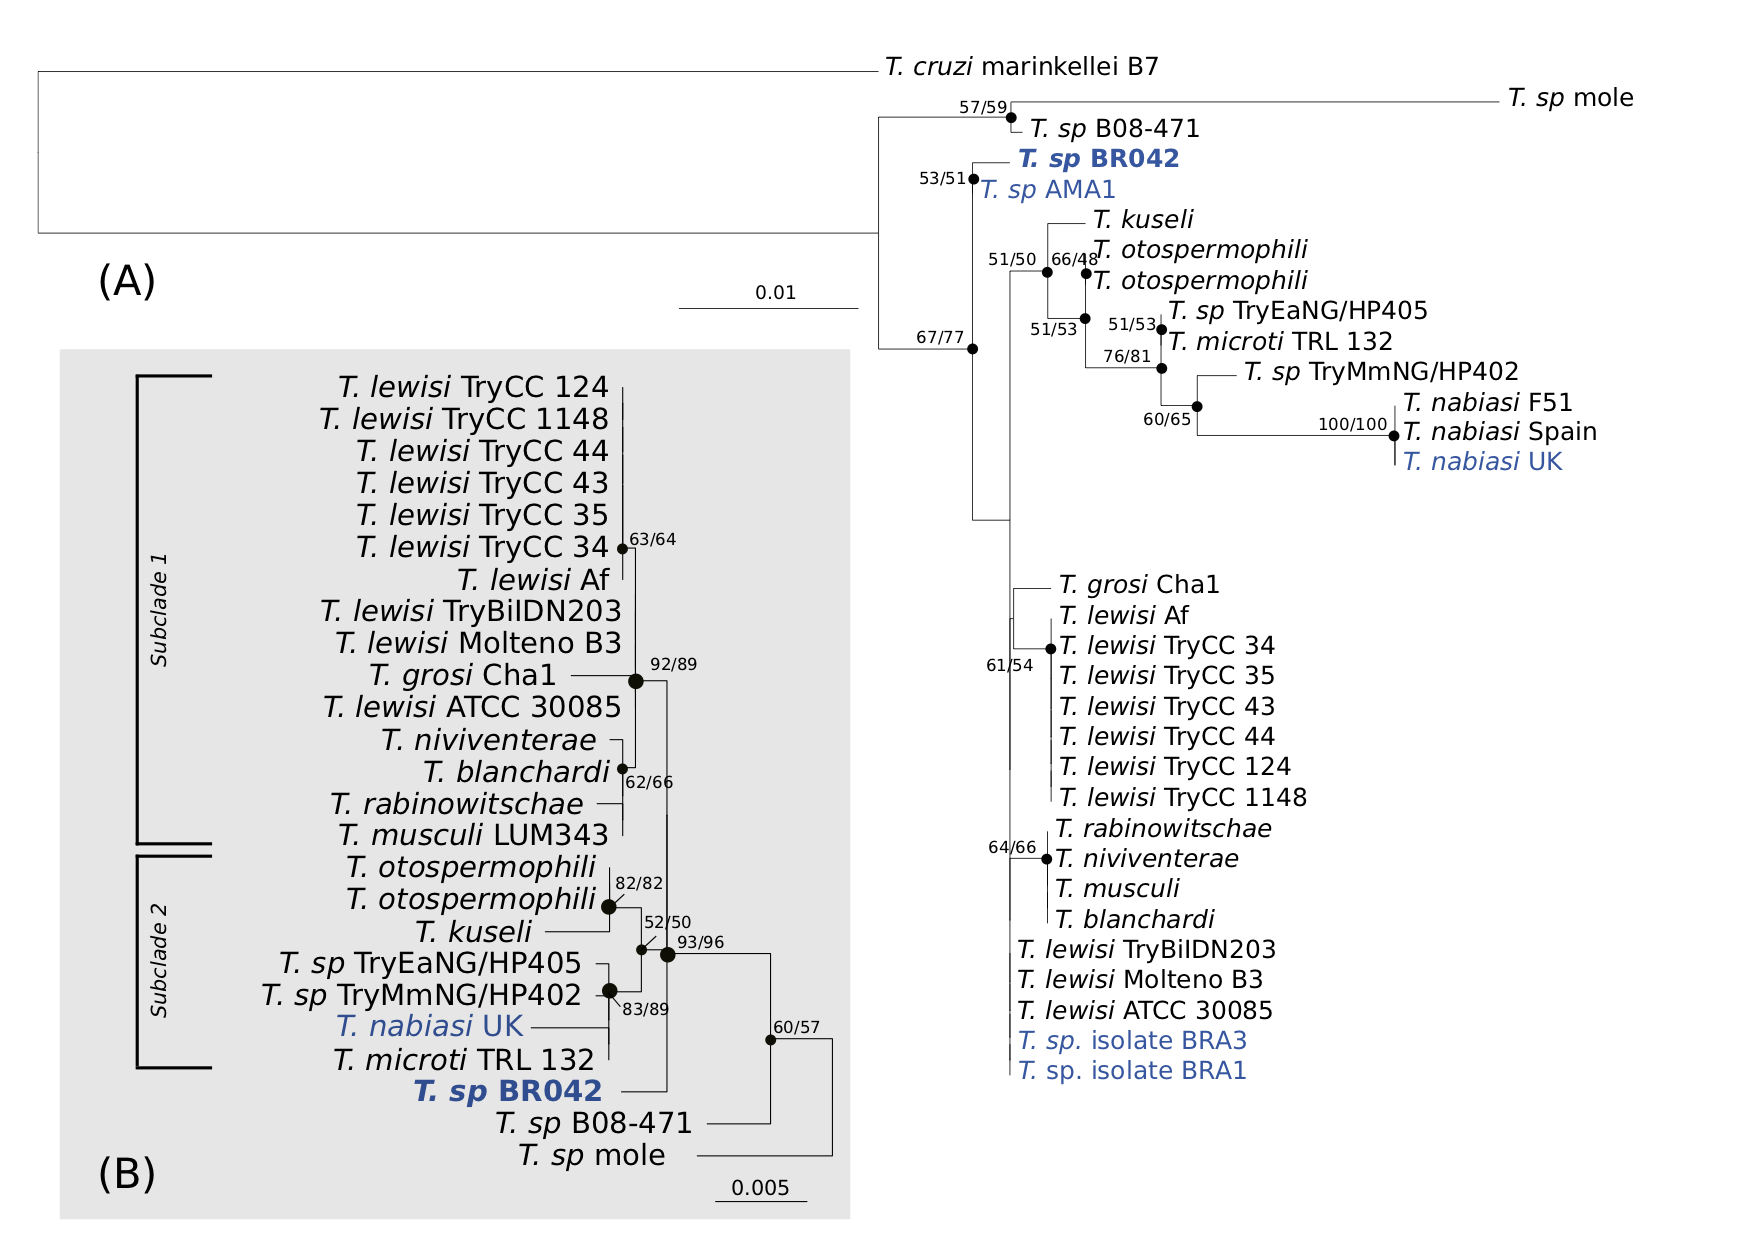
\includegraphics[width=0.95\linewidth]{figures/ms-figs/Ch5-Fig1} \caption[Phylogeny of \textit{Trypanosoma Herpetosoma} subgenus based on the 18S rRNA locus.]{Maximum likelihood phylogenetic reconstruction of \textit{Trypanosoma Herpetosoma} subgenus based on the 18S rRNA locus. Evolutionary relationship inferred using the Kimura 2-parameter (K2P) + G substitution model with 1,000 bootstrap replicates. Node support values shown for ML and Neighbour-Joining (NJ) analyses respectively, values <50 have been hidden. All positions containing gaps and missing data were eliminated. (a) phylogeny based on short alignment (483 bp) of V7-8 hyper-variable region of the 18S locus (b) phylogeny based on longer alignment (1,491 bp) of 18S locus, outgroup to \textit{Tr. cruzi} (AJ009150) not shown. Number of substitutions per nucleotide position is represented by the scale bar. New sequence from the present study is designated in bold. Sequences from Australia in blue \textit{Tr. nabiasi} UK isolate (AJ843896) is identical to sequences obtained from Australian wild rabbits (\textit{O. cuniculus}) and their fleas (\textit{S. cuniculi}) (see Hamilton et al., 2005).}\label{fig:F51}
\end{figure}

Phylogenetic analysis of the shorter (483 bp) 18S rRNA gene alignment was used in order to include a greater variety of reference sequences, in particular for the context of the present study to include the only other \emph{Tr. lewisi}-like sequences from Australia \autocite{hamiltonInadvertentIntroductionAustralia2005,averisDiversityDistributionHostparasite2009}. Figure \ref{fig:F51} shows the phylogeny of the \emph{Trypanosoma} \emph{Herpetosoma} subgenus. As demonstrated by the polytomy present in Figure \ref{fig:F51}a, this short region of the 18S rRNA gene is insufficient in the differentiation of members within the \emph{Tr. lewisi} clade. Due to the speed at which the 18S rRNA locus has evolved, short regions of this locus have been reported as being unsuitable for inference of evolutionary relationships between \emph{Trypanosoma} species \autocite{hamiltonResolvingRelationshipsAustralian2011}.

Reconstruction of phylogenetic relationships over a longer region (1,491 bp) of the 18S rRNA gene exhibited superior resolution within the \emph{Tr. lewisi} clade Figure \ref{fig:F51}b. In this phylogeny, sequences obtained from Australian black rats in the present study did not fall within the \emph{Tr. lewisi} sensu stricto clade; instead they formed a distinct group of sequences that branched separately from other reference sequences. Pairwise distance analysis over a 1,491 bp alignment of the 18S rRNA gene demonstrated sequences from the black rat were 99.5\% similar to \emph{Trypanosoma microti} (AJ009158). The next most similar sequences were \emph{Trypanosoma} sequences from voles in Japan (AB242275, AB242276) and a flea from Czech Republic (KF054111), all of which were 99.4\% similar. Members of the \emph{Tr. lewisi} sensu stricto clade, as shown in Figure \ref{fig:F52}, were all 100\% identical to each other over the 1,491 bp alignment. These were the third most similar sequences (99.3\%) to the \emph{Trypanosoma} sp. identified in the present study. Inspection of a 433 bp alignment at the V7-8 18S hyper-variable region (Figure \ref{fig:F52}), demonstrated that the most similar trypanosome sequence to that obtained in this study were those from a native Australian mouse in the south-west of Western Australia (\emph{Pseudomys albocinereus}) (FJ823119) with seven single nucleotide polymorphisms (SNPs).

The phylogeny in the present study supports previous research by Hamilton et al. \autocite*{hamiltonInadvertentIntroductionAustralia2005} that demonstrated the \emph{Tr. lewisi} clade can be divided into two subclades, consisting of \emph{Tr. lewisi}, \emph{Tr. musculi}, \emph{Tr. rabinowitschae}, \emph{Tr. blanchardi} and \emph{Tr. grosi} in subclade one and \emph{Tr. nabiasi}, \emph{Tr. microti}, and \emph{Tr. otospermophili} in subclade two. Trypanosome sequences obtained in the present study from Australian black rats form a paraphyletic group to the two monophyletic \emph{Tr. lewisi} clades. Despite the basal position in the phylogenetic tree, genetic distances show a high similarity to \emph{Tr. lewisi} subclade two.

\begin{figure}
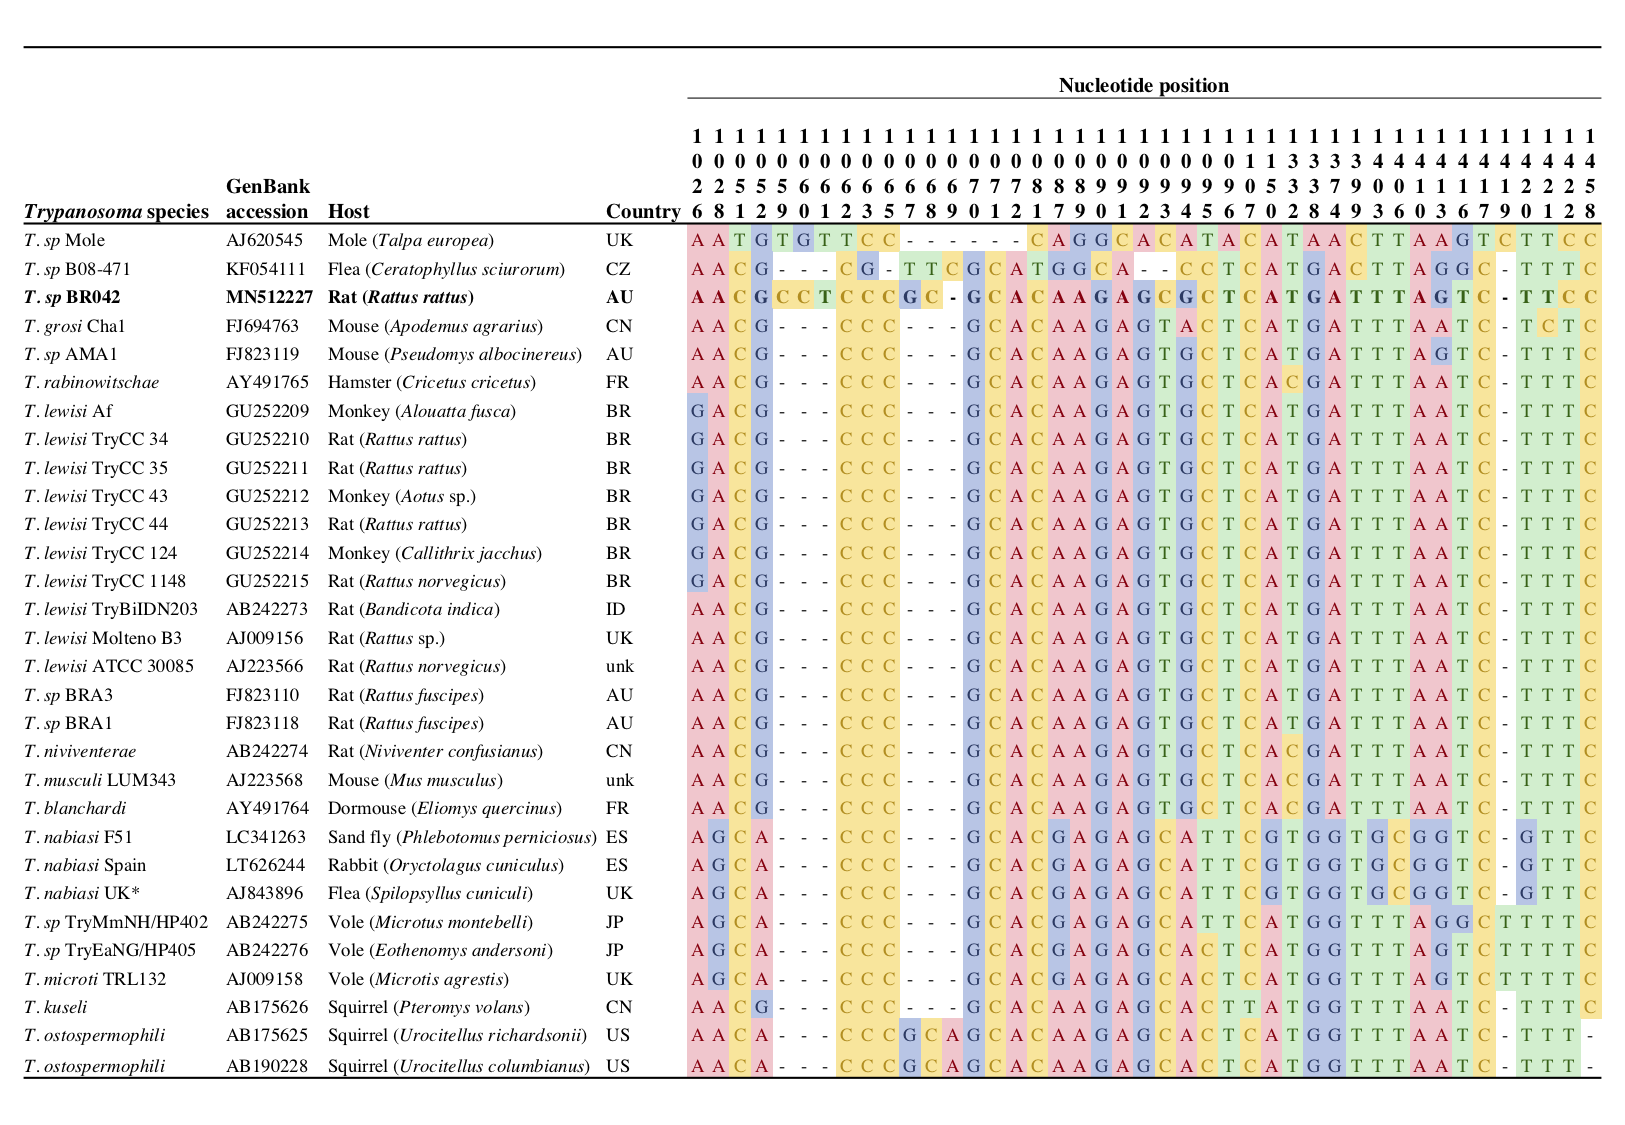
\includegraphics[width=0.95\linewidth]{figures/ms-figs/Ch5-Fig2} \caption[Nucleotide alignment of \textit{Trypanosoma lewisi} clade.]{Polymorphic sites within the V7-8 hyper-variable region of the 18S rRNA locus (433 bp) for trypanosomes of the subgenus \textit{Herpetosoma}. \textit{Tr. nabiasi} UK isolate (AJ843896) is identical to sequences obtained from Australian wild rabbits (\textit{O. cuniculus}) and their fleas (\textit{S. cuniculi}) (see Hamilton et al., 2005). Country abbreviations; Australia (AU), Brazil (BR), China (CN), Czech Republic (CZ), France (FR), Indonesia (ID), Japan (JP), Spain (ES), United Kingdom (UK), United States of America (US), unknown (unk).}\label{fig:F52}
\end{figure}

Morphological identification of rodent trypanosomes in Australia, attributed to \emph{Tr. lewisi}, was first made by T. L. Bancroft in 1888 in black rats in Brisbane \autocite{mackerrasHaematozoaAustralianMammals1959}, with subsequent records by various scientists who confirmed the presence of this parasite in; Brisbane by Pound (1905), in Perth by Cleland (1906, 1908), and in Sydney by Johnston (1909) (all cited by Mackerras \autocite*{mackerrasHaematozoaAustralianMammals1959}). Trypanosomes presumed to be \emph{Trypanosoma} \emph{lewisi} were first identified in native Australian fauna by Mackerras \autocite*{mackerrasCatalogueAustralianMammals1958a}. Morphological detection of the parasite has been made from the bush rat (\emph{Rattus fuscipes}; Queensland) and the water rat (\emph{Hydromys chrysogaster}; Queensland) \autocite{mackerrasHaematozoaAustralianMammals1959,mackerrasCatalogueAustralianMammals1958a}. More recently, molecular reports of \emph{Trypanosoma} species from the \emph{Tr. lewisi} clade have been made from native wildlife in Western Australia, including two bush rats (\emph{Rattus fuscipes}), a dibbler (\emph{Parantechinus apicalis}) and an ash-grey mouse (\emph{Pseudomys albocinereus}) \autocite{averisDiversityDistributionHostparasite2009}. Interestingly, despite sampling from 371 native mammals, 19 different species and 14 sites, detection of \emph{Tr. lewisi}-like species was confined only to mammals from Fitzgerald River in the south-west of Australia. The identification of \emph{Tr. lewisi}-like spp. by Averis et al. \autocite*{averisDiversityDistributionHostparasite2009} was limited by the short size of the 18S rRNA gene analysed (444 bp). As demonstrated in the present study, across a short region of the 18S rRNA gene, trypanosomes within the \emph{Tr. lewisi} clade can share a high sequence similarity (Figure \ref{fig:F51}), however upon more robust analysis of a longer fragment it is evident that sequences within the \emph{Tr. lewisi} clade form distinct groups. Additional genetic information (e.g.~glycosomal glyceraldehyde-3-phosphate dehydrogenase (gGAPDH)) will also assist in determining the phylogenetic relationships of these closely related species in future studies.

The genetic relationship of the Australian isolate BR042 to \emph{Tr. microti}, a trypanosome isolated from a vole (\emph{Microtis agrestis}) in England suggest that the \emph{Tr. lewisi} isolates from this study are closely related to rodent trypanosomes in the subgenus \emph{Herpetosoma} from Europe. This agrees with finding by Hamilton et al. \autocite*{hamiltonEvolutionTrypanosomaCruzi2012} reporting that Australian trypanosomes appear to be more closely related to trypanosomes outside of Australia than to each other. This observation is consistent with the hypothesis that some trypanosomes have been introduced into the Australian continent comparatively recently, rather than this trypanosome evolving in Australia following the breakup of Gondwana; \emph{Trypanosoma lewisi} (known to be host specific) likely arrived in Australia with black rats when individuals colonised the mainland. Additionally, Hamilton et al. \autocite*{hamiltonInadvertentIntroductionAustralia2005} detected European \emph{Tr. nabiasi} (from the \emph{Tr. lewisi} clade) in Australian wild rabbits (\emph{Oryctolagus cuniculus}) suggesting that these parasites may have been brought into Australia with the first 24 rabbits introduced from England in 1859 \autocite{hamiltonInadvertentIntroductionAustralia2005}.

The introduction of black rats and their associated trypanosomes to regions previously free of these species has long been considered responsible for the extinction of two native rat species \emph{Rattus macleari} and \emph{Rattus nativitatis}, as occurred on Christmas Island (an island Australian Territory located in the Indian Ocean, south of Indonesia) \autocite{wyattHistoricalMammalExtinction2008}. Recent research has since concluded that the rapid decline and extinction of the two endemic rat species was correctly attributed to infections with \emph{Tr. lewisi} \autocite{wyattHistoricalMammalExtinction2008}. A review of historical records demonstrated a rapid extinction event following the arrival of black rats on the island in September 1900 and an absence of native rat sightings by October 1904 \autocite{greenMammalExtinctionIntroduced2014}. A recent study by Dybing et al. \autocite*{dybingGhostsChristmasAbsence2016} investigated the presence of \emph{Trypanosoma} and \emph{Leishmania} spp. from feral cats (\emph{Felis catus}) and black rats (\emph{R. rattus}) on Christmas Island. Through molecular analysis of spleen samples, the study did not detect any \emph{Trypanosoma} or \emph{Leishmania} species. In addition, the same study reported an absence of these parasites from feral cat samples from Dirk Hartog Island and sites from south-west Western Australia.

North Head is situated at the entrance to the Sydney harbour and is dominated by Eastern Suburbs banksia scrub, an endangered ecological community \autocite{perkinsEasternSuburbsBanksia2012}. Following European arrival, the headland was used to quarantine arriving ship passengers. In addition to being home to endangered populations of long-nosed bandicoots (\emph{Perameles nasuta}) and little penguins (\emph{Eudyptula minor}), reintroductions of native fauna species, such as bush rats (\emph{Rattus fuscipes}), eastern pygmy possums (\emph{Cercartetus nanus}) and brown antechinus (\emph{Antechinus stuartii}), have also occurred at this site. While, to date, there is no evidence of a spill-over of trypanosomes within the \emph{Tr. lewisi} clade to native species, ongoing monitoring of such populations is advised given the historical significance of this parasite with respect to native animal declines \autocite{greenMammalExtinctionIntroduced2014,wyattHistoricalMammalExtinction2008}.

In addition to trypanosomes, black rats may act as reservoirs for many other sources of infectious agents \autocite{banksReviewEvidencePotential2012}. Additional information regarding the presence, distribution and diversity of pathogens harboured by black rats in Australia is critical to understanding the dynamics of pathogen spill-over \autocite{beckerDynamicIntegrativeApproaches2019}. Future research encompassing both morphological and molecular techniques is on-going by the authors. Collection of ectoparasites, blood, and tissue samples from both native and introduced wildlife will likely continue to shed light on the diversity and distribution of vector-borne microorganisms impacting wildlife, domestic animals and humans.

\hypertarget{tas-devil}{%
\chapter{Tasmanian devil haemoprotozoa}\label{tas-devil}}

\chaptermark{Devil haemoprotozoa}

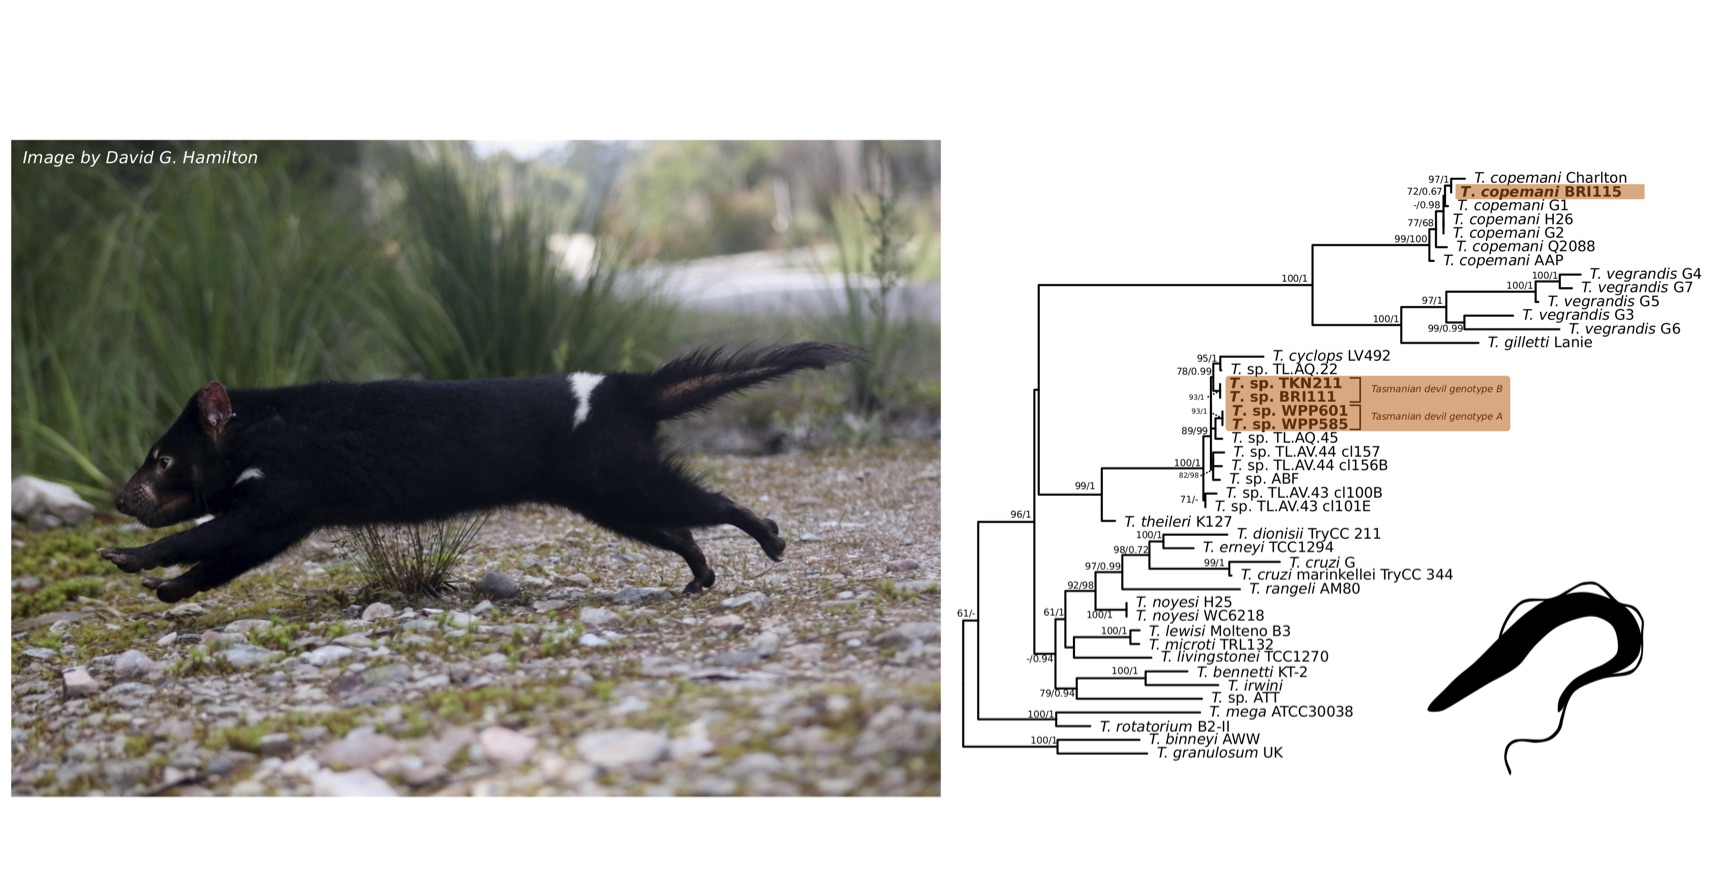
\includegraphics[width=1\linewidth]{front-and-back-matter/preface/tasdevil}

\newpage

\hypertarget{preface-5}{%
\section*{Preface}\label{preface-5}}
\addcontentsline{toc}{section}{Preface}

\textbf{Attribution Statement}

The following chapter has been drafted in accordance with the journal \emph{Pathogens}.

The following manuscript has been published: \textbf{Egan, S.}, Ruiz-Aravena, M., Austen, J., Barton, X., Comte, S., Hamilton, D., Hamede, R., Ryan, U., Irwin, P., Jones, M., and Oskam, C. \emph{2020}. Blood parasites in endangered wildlife: trypanosomes discovered during a survey of haemoprotozoa from the Tasmanian devil. \emph{Pathogens}, \textbf{9}(11), 873. DOI: \href{https://doi.org/10.3390/pathogens9110873}{10.3390/pathogens9110873}

The following authors contributed to this manuscript as outlined below\footnote{Contribution indicates the total involvement the author has had in this project. Placing an `X' in the remaining boxes indicates what aspect(s) of the project each author engaged in.}.

\begin{table}[!h]
\centering\begingroup\fontsize{7}{9}\selectfont

\begin{tabular}{lrllll}
\toprule
Authorship order & Contribution (\%) & Concept Development & Data Collection & Data Analysis & Draft\\
\midrule
\cellcolor{gray!6}{Siobhon L. Egan} & \cellcolor{gray!6}{70} & \cellcolor{gray!6}{X} & \cellcolor{gray!6}{X} & \cellcolor{gray!6}{X} & \cellcolor{gray!6}{X}\\
Manuel Ruiz-Aravena & 5 & X &  &  & \\
\cellcolor{gray!6}{Jill M. Austen} & \cellcolor{gray!6}{2} & \cellcolor{gray!6}{} & \cellcolor{gray!6}{} & \cellcolor{gray!6}{X} & \cellcolor{gray!6}{}\\
Xavier Barton & 2 &  & X &  & \\
\cellcolor{gray!6}{Sebastien Comte} & \cellcolor{gray!6}{2} & \cellcolor{gray!6}{} & \cellcolor{gray!6}{X} & \cellcolor{gray!6}{} & \cellcolor{gray!6}{}\\
David G. Hamilton & 2 &  & X &  & \\
\cellcolor{gray!6}{Robrigo K. Hamede} & \cellcolor{gray!6}{2} & \cellcolor{gray!6}{} & \cellcolor{gray!6}{X} & \cellcolor{gray!6}{} & \cellcolor{gray!6}{}\\
Una M. Ryan & 4 & X &  &  & \\
\cellcolor{gray!6}{Peter J. Irwin} & \cellcolor{gray!6}{4} & \cellcolor{gray!6}{X} & \cellcolor{gray!6}{} & \cellcolor{gray!6}{} & \cellcolor{gray!6}{}\\
Menna E. Jones & 2 & X &  &  & \\
\cellcolor{gray!6}{Charlotte L. Oskam} & \cellcolor{gray!6}{5} & \cellcolor{gray!6}{X} & \cellcolor{gray!6}{} & \cellcolor{gray!6}{} & \cellcolor{gray!6}{}\\
\bottomrule
\end{tabular}
\endgroup{}
\end{table}

By signing this document, the Candidate and Principal Supervisor acknowledge that the information provided is accurate and has been agreed to by all other authors.

\vspace{3mm}

\raggedright

\_\_\_\_\_\_\_\_\_\_\_\_\_\_\_\_\_\_ ~ ~ ~ \_\_\_\_\_\_\_\_\_\_\_\_\_\_\_\_\_\_\\
\hspace*{0.333em}\hspace*{0.333em}Candidate ~ ~ ~ ~ ~ ~ ~ ~ ~ ~ ~ ~ ~ ~ ~ ~ Principal Supervisor

\newpage

\textbf{Chapter linking statement:}
This chapter comprises a collaborative research project with the University of Tasmania. The Tasmanian devil is the largest extant carnivore and experience devastating declines due to a transmissible cancer known as devil facial tumour disease (DFTD). In this study we provide the first molecular survey of blood parasites in the Tasmanian devil. This research provide important important insights into the diversity of haemoprotozoa and ground work for future research to further understand the clinical impacts and interactions with DFTD. In addition in the broader context of this thesis this research is also of interest into zoonoses, and builds on the theme of wildlife surveillance. As as large carnivore devils fill a unique niche and could serve as an important reservoir for zoonotic pathogens. These findings further add to research that shows Australian wildlife harbor unique parasites that are endemic to Australia and surrounds, adding the growing research that Australia is free of many known pathogens described over seas.

\vspace{5mm}

\textbf{Acknowledgement statement:}
We thank Sarah Munns for extraction of DNA and A/Prof Chris Peacock (The University of Western Australia) for provision of \emph{Leishmania macropodum} control. We acknowledge the generous support of the large number of volunteers who assisted with fieldwork and data collection.

\vspace{5mm}

\textbf{Funding statement:} This study was part-funded by the Australian Research Council (LP160100200), Bayer HealthCare (Germany) and Bayer Australia. S.L.E. was supported by an Australian Government Research Training Program (RTP) Scholarship. This project was also part supported by The Holsworth Wildlife Research Endowment \& The Ecological Society of Australia (awarded to S.C. and S.L.E). Fieldwork and data collection were funded by the US National Institute of Health (R01-GM126563-01), the Save the Tasmanian Devil Appeal of the University of Tasmania Foundation (Eric Guiler Grant Scheme) and the Australian Research Council (DE170101116).

\vspace{5mm}

\textbf{Data availability:} Sequences generated in the present study have been submitted to GenBank nucleotide database under accession numbers MT883295 -- MT883326 (trypanosome \emph{18S rRNA}), MT514664 -- MT514666 (trypanosome \emph{GAPDH}) and MW084364 (\emph{Babesia} \emph{18S rRNA}).

\vspace{5mm}

\textbf{Keywords:} Tasmanian devil; \emph{Sarcophilus harrisii}; Haemoprotozoa; \emph{Trypanosoma}; Marsupial; Devil facial tumour disease (DFTD)

\newpage

\hypertarget{abstract-4}{%
\section{Abstract}\label{abstract-4}}

The impact of emerging infectious diseases is increasingly recognised as a major threat to wildlife. Wild populations of the endangered Tasmanian devil, \emph{Sarcophilus harrisii}, are experiencing devastating losses from a novel transmissible cancer, devil facial tumour disease (DFTD), however, despite the rapid decline of this species there is currently no information on the presence of haemoprotozoan parasites. In the present study, 95 Tasmanian devil blood samples were collected from four populations in Tasmania, Australia, which underwent molecular screening to detect four major groups of haemoprotozoa: (i) trypanosomes, (ii) piroplasms, (iii) \emph{Hepatozoon} and (iv) haemosporidia. Sequence results revealed \emph{Trypanosoma} infections in 32/95 individuals. \emph{Trypanosoma copemani} was identified in 10 Tasmanian devils from three sites and a second \emph{Trypanosoma} sp. was identified in 22 individuals that grouped within the poorly described \emph{Tr. cyclops} clade. A single blood sample was positive for \emph{Babesia} sp. that most closely matched \emph{Babesia lohae}. No other blood protozoan parasite DNA was detected. This study provides the first insight into haemoprotozoa from the Tasmanian devil and the first identification of \emph{Trypanosoma} and \emph{Babesia} in this carnivorous marsupial.

\hypertarget{introduction-4}{%
\section{Introduction}\label{introduction-4}}

Haemoprotozoan parasites are unicellular eukaryotic organisms with complex lifecycles involving an invertebrate vector and often alternate in their tropism between the tissues and the blood of their vertebrate hosts. Four major haemoprotozoan assemblages infect mammals \autocite{odonoghueHaemoprotozoaMakingBiological2017}; (i) Trypanosomatids (Kinetoplastea), which are flagellated protists characterised by the presence of a unique organelle, the kinetoplast; (ii) haemogregarines (Adeleorina); (iii) haemosporidia (Haemosporidia); and (iv) piroplasms (Piroplasmida). Broadly haemoprotozoans are considered either host specific (e.g.~\emph{Theileria ornithorhynchi} infecting the platypus (\emph{Ornithorhynchus anatinus}) host \autocite{papariniFirstMolecularCharacterization2015}) or generalists (e.g.~\emph{Trypanosoma cruzi} which infects a wide range of mammals \autocite{clementOutAfricaOrigins2020}). However, the true diversity and epidemiology of most of these species remains unknown.

The Tasmanian devil, \emph{Sarcophilus harrisii}, is the largest extant marsupial carnivore. Once present across mainland Australia (\textasciitilde3,000 years ago), the distribution of wild populations of Tasmanian devils became restricted to the island of Tasmania \autocite{bruniche-olsenAncientDNATracks2018}, off the southern coast of the Australian mainland. Biogeographical events have influenced declines in the effective size of devil populations and their distribution, with consequential genetic bottleneck resulting in low genetic diversity \autocite{jonesGeneticDiversityPopulation2004,bruniche-olsenAncientDNATracks2018,pattonContemporaryDemographicReconstruction2019}. Since 1996, a transmissible cancer (devil tumour facial disease, DFTD hereafter) gradually spread across most of the distributional range of the species and caused local population declines of upwards of 80\% \autocite{mccallumTransmissionDynamicsTasmanian2009,lazenbyDensityTrendsDemographic2018}. Transmission of DFTD occurs through direct transfer of live tumour cells between individuals when devils bite each other during social interactions \autocite{pearseAllograftTheoryTransmission2006,hamedeBitingInjuriesTransmission2013,hamiltonRateIntersexualInteractions2019}. Survival in DFTD infected individuals is usually 6-12 months after clinical signs appear; the disease is lethal in almost 100\% of cases \autocite{pyeDevilFacialTumor2016}. As a consequence of transmission being driven by social interactions, DFTD is still present even in largely depleted populations of hosts \autocite{mccallumTransmissionDynamicsTasmanian2009}. Therefore, any additional pressure(s) on the host health, such as co-infections with haemoparasites, could further threaten imperilled populations, yet, little is known about the devil's parasite community \autocite{waitReviewParasitesTasmanian2017}.

To date, only four protozoan parasite groups have been identified from wild devil populations; \emph{Cryptosporidium} spp., \emph{Giardia} spp., \emph{Toxoplasma gondii} and \emph{Sarcocystis} sp. A previous study identified sporulated sporocysts consistent with \emph{Sarcocystis} (family: Sarcocystidae) species from the intestinal mucosa using microscopic examination \autocite{mundaySarcocystisRelatedOrganisms1978}. In north-west Tasmania, \emph{T. gondii} prevalence was higher in carnivorous marsupials such as the Tasmanian devil, spotted-tail quoll (\emph{Dasyurus maculatus}) and eastern quoll (\emph{D. viverrinus}), compared to sympatric prey marsupials like the brushtail possum (\emph{Trichosurus vulpecula}), Bennett's wallaby (\emph{Notamacropus rufogriseus}, syn. \emph{Macropus rufogriseus}) and Tasmanian pademelon (\emph{Thylogale billardierii}) \autocite{hollingsWildlifeDiseaseEcology2013}. Recently, \emph{Cryptosporidium} and \emph{Giardia} spp. were also identified from faecal samples of wild devils using molecular techniques \autocite{waitMolecularCharacterizationCryptosporidium2017}.

Over the past two decades the use of molecular techniques has significantly extended our understanding of haemoprotozoan parasites. As a result, it has revealed that Australian marsupials and monotremes can host a high diversity of haemoprotozoa species, most of which are unique to Australia \autocite{thompsonTrypanosomesAustralianMammals2014,austenInvestigationMorphologicalDiversity2015,barbosaSequenceAnalysesMitochondrial2019,northoverIncreasedTrypanosomaSpp2019}. The clinical effects of co-infections in wildlife are often difficult to evaluate. One well documented case is the investigation into a canine distemper virus epidemic in Serengeti lions (\emph{Panthera leo}), which identified that joint infection by haemoprotozoa was a major contributing factor to fatal outcomes \autocite{munsonClimateExtremesPromote2008}. While there are limited studies on the clinical and pathological consequences of such interactions in native Australian wildlife, there is evidence that co-infection and co-morbidities can place species at an increased risk of disease when challenged with infection of haemoprotozoa \autocite{mcinnesPotentialImpactNative2011,boteroTrypanosomesGeneticDiversity2013,thompsonTemporalSpatialDynamics2014}.

The present study aimed to screen blood samples from Tasmanian devils for the presence of haemoprotozoan parasites. To the authors' knowledge the present study provides the first survey of haemoprotozoa from Tasmanian devils.

\hypertarget{materials-and-methods}{%
\section{Materials and Methods}\label{materials-and-methods}}

\hypertarget{study-sites-and-sampling}{%
\subsection{Study sites and sampling}\label{study-sites-and-sampling}}

Animal use was approved by the University of Tasmania Animal Ethics Committee permit numbers A0015835 and A0016789) and the Department of Primary Industries, Parks, Water and Environment Animal Ethics Committee (permit numbers TFA19144 and TFA18028).

A total of 95 blood samples were collected from wild Tasmanian devils captured during the austral autumn (May 2018) from four sites across Tasmania: Black River, Takone, West Pencil Pine and Freycinet (Figure \ref{fig:F61}). The sampling effort at each site involved deployment of 40 PVC pipe traps during 7 to 10 consecutive nights. Individual devils were identified via subcutaneously implanted microchips (AllFlex\(\copyright\) ISO FDX-B).

Blood was collected (between 0.3-1 mL) from either the jugular vein (Takone) or marginal ear vein (Black River, Freycinet and West Pencil Pine). The puncture site was disinfected with sterile alcohol swabs for at least 15 seconds prior to collection and blood was stored in ethylenediaminetetraacetic acid (EDTA) vacutainers. Samples were kept refrigerated at 4\(^\circ\)C and shipped to Murdoch University, Western Australia where they were stored at -20\(^\circ\)C until analysis.

\begin{figure}
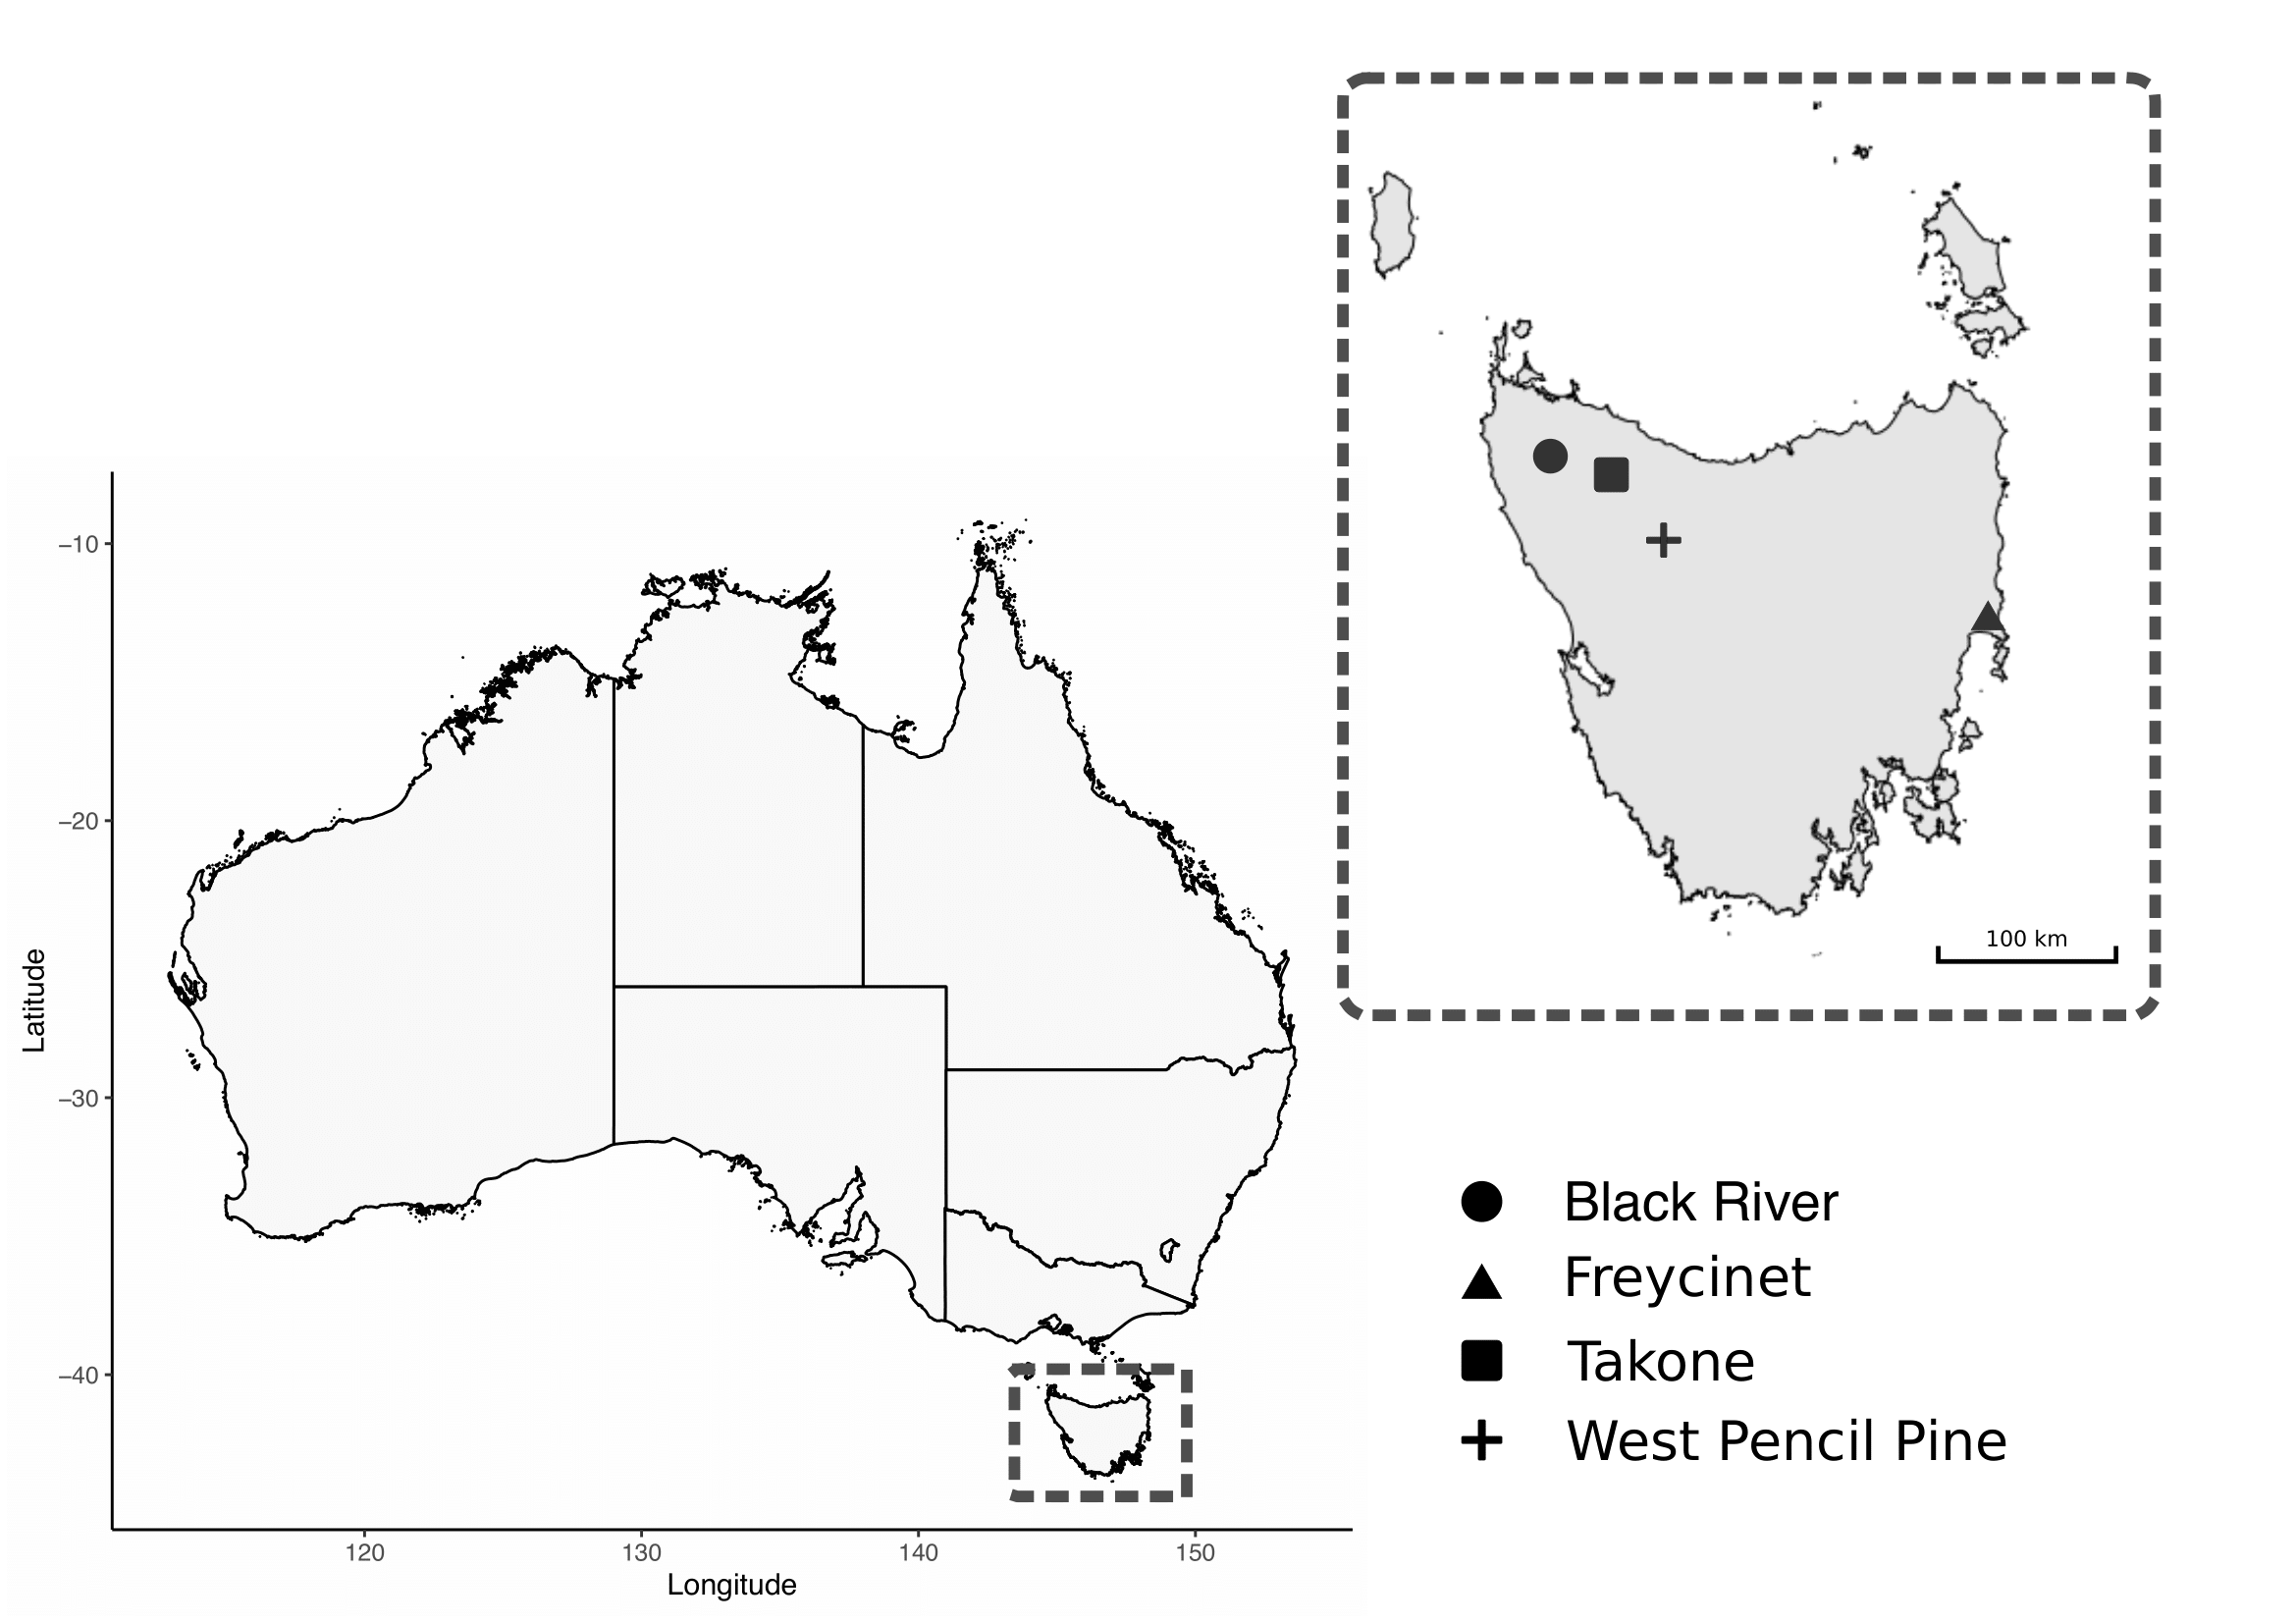
\includegraphics[width=0.95\linewidth]{figures/ms-figs/Ch6-Fig1} \caption[Map of study sites for Tasmanian devil.]{Map of study sites for field collection of Tasmanian Devil \textit{Sarcophilus harrisii}.}\label{fig:F61}
\end{figure}

\hypertarget{molecular-screening}{%
\subsection{Molecular screening}\label{molecular-screening}}

\hypertarget{dna-extraction}{%
\subsubsection{DNA extraction}\label{dna-extraction}}

Total genomic DNA was extracted from 200 \(\mu\)L of blood using a MasterPure DNA purification kit (Epicentre\textregistered Biotechnologies, Madison, Wisconsin, U.S.A) following the manufacturer's recommendations. Where 200 \(\mu\)L of blood was not available, sterile DNA free phosphate-buffered saline (PBS) was used to make samples up to 200 \(\mu\)L. Genomic DNA (gDNA) was eluted in 30 \(\mu\)L of TE buffer and stored at -20\(^\circ\)C. Extraction controls (EXBs) consisting of 200 \(\mu\)L sterile DNA free PBS, were included randomly in each extraction batch (N=7).

\hypertarget{pcr-assays}{%
\subsubsection{PCR assays}\label{pcr-assays}}

Molecular screening was carried out for haemoprotozoa on gDNA from blood samples (N=95) and EXBs (N=7). Reactions were carried out in 25 \(\mu\)L volumes containing 2 \(\mu\)L of gDNA or 1 \(\mu\)L of the primary product for nested and semi-nested PCR assays. An overview of assays, including primer sequences, is available in Table \ref{tab:T61}.



\begin{table}

\caption[Primers used for haemoprotozoa screening of Tasmanian devils.]{\label{tab:T61}List of primers used for screening of haemoprotozoa from Tasmanian Devils (\emph{Sarcophilus harrisii}). References: \textbf{1.} McInnes et al. \autocite*{mcinnesTrypanosomaIrwiniSp2009}, \textbf{2.} Maslov et al. \autocite*{maslovPhylogenyTrypanosomesInferred1996}, \textbf{3.} Jefferies et al. \autocite*{jefferiesPCRRFLPDetectionDifferentiation2007}, \textbf{4.} Ujvari et al. \autocite*{ujvariHighPrevalenceHepatozoon2004}, \textbf{5.} Waldenstrom et al. \autocite*{waldenstromNewNestedPolymerase2004}, \textbf{6.} Bensch et al. \autocite*{benschHostSpecificityAvian2000}.}
\centering
\fontsize{8.5}{10.5}\selectfont
\begin{tabular}[t]{llllr}
\toprule
Target & Primer & Sequence & Size & Reference\\
\midrule
\textbf{Trypanosomes} & \textbf{} & \textbf{} & \textbf{} & \textbf{}\\
18S primary SSU & SLF & GCTTGTTTCAAGGACTTAGC & \textasciitilde{}1.5 kb & 1\\
18S primary SSU & S762R & GACTTTTGCTTCCTCTAATG &  & 2\\
18S secondary SSU2 & S823F & CGAACAACTGCCCTATCAGC & \textasciitilde{}904 bp & 2\\
18S secondary SSU2 & 662R & GACTACAATGGTCTCTAATC &  & 2\\
18S secondary SSU1 & S825F & ACCGTTTCGGCTTTTGTTGG & \textasciitilde{}959 bp & 2\\
18S secondary SSU1 & SLIR & ACATTGTAGTGCGCGTGTC &  & 1\\
GAPDH Primer & GAPDHF & CTYMTCGGNAMKGAGATYGAY & \textasciitilde{} 900 bp & 1\\
GAPDH Primer & GAPDHR & GRTKSGARTADCCCCACTCG &  & 1\\
GAPDH Secondary & GAPDHF & CTYMTCGGNAMKGAGATYGAY & \textasciitilde{} 880 bp & 1\\
GAPDH Secondary & Ga4 & GTTYTGCAGSGTCGCCTTGG &  & 1\\
\textbf{Piroplasms} & \textbf{} & \textbf{} & \textbf{} & \textbf{}\\
18S primary & BT1F & GGCTCATTACAACAGTTATAG & \textasciitilde{} 900 bp & 3\\
18S primary & BT1R & CCCAAAGACTTTGATTTCTCTC &  & 3\\
18S secondary & BT2F & CCGTGCTAATTGTAGGGCTAAT & \textasciitilde{} 800 bp & 3\\
18S secondary & BT2R & GGACTACGACGGTATCTGATCG &  & 3\\
\textbf{Hepatozoon} & \textbf{} & \textbf{} & \textbf{} & \textbf{}\\
18S & HepF300 & GTTTCTGACCTATCAGCTTTCGACG & \textasciitilde{}600 bp & 4\\
18S & Hep900 & CAAATCTAAGAATTTCACCTCTGAC &  & 4\\
\textbf{Haemosporidia} & \textbf{} & \textbf{} & \textbf{} & \textbf{}\\
Cytb primary & HaemNF & CATATATTAAGAGAATTATGGAG & \textasciitilde{}580 bp & 5\\
Cytb primary & HaemNR2 & AGAGGTGTAGCATATCTATCTAC &  & 5\\
Cytb secondary & HaemF & ATGGTGCTTCGATATATGCATG & \textasciitilde{}520 bp & 6\\
Cytb secondary & HaemR2 & GCATTATCTGGATGTGATAATGGT &  & 6\\
\bottomrule
\end{tabular}
\end{table}

For identification of trypanosomes (\emph{Trypanosoma} and \emph{Leishmania} spp.) samples were screened using a nested PCR assay targeting an \textasciitilde959 bp product of the second half of the 18S ribosomal RNA (18S rRNA) locus. This assay amplifies most species of \emph{Trypanosoma} \autocite{mcinnesTrypanosomaIrwiniSp2009} and was also validated in the present study to amplify \emph{Leishmania} spp. using control gDNA of \emph{Leishmania infantum} from a canine bone marrow sample and \emph{Leishmania macropodum} culture isolate. External primers SLF/S762R and internal primers S825F/SLIR were used as an initial screen and sequenced as per details below. Samples representative of the different genotypes identified then underwent an additional secondary assay with a second set of internal primers S823/S662R to yield a near full length \emph{18S rRNA} sequence. Reactions were carried out in 25 \(\mu\)L volumes containing 0.4 \(\mu\)M of each primer and 12.5 \(\mu\)L GoTaq\textregistered Green master mix (Promega, U.S.A.). Thermal cycling conditions were as follows; initial cycle of 95\(^\circ\)C for 5 mins, 50\(^\circ\)C for 2 mins, 72\(^\circ\)C for 4 mins, followed by 35 cycles of 95\(^\circ\)C for 30 secs, 52\(^\circ\)C (primary) or 55\(^\circ\)C (secondary) for 30 secs, 72\(^\circ\)C for 2 mins 20 secs (primary) or 1 min (secondary), and a final extension of 72\(^\circ\)C for 5 mins. To obtain further phylogenetic information from the genotypes identified by 18S rRNA locus screening, samples underwent amplification of the glycosomal Glyceraldehyde Phosphate Dehydrogenase (\emph{gGAPDH}) gene using a semi-nested PCR assay with external primers GAPDHF/GAPDHR and internal primers GAPDHF/Ga4 \autocite{mcinnesTrypanosomaIrwiniSp2009}. Reactions contained 1X buffer (KAPA Biosystems, South Africa), 2.0 mM MgCl\textsubscript{2}, 0.4 \(\mu\)M of each primer, 0.25 mM of each dNTP, and 0.5 U of Taq (KAPA Biosystems, South Africa). Thermal cycling conditions were as follows; initial cycle of 95\(^\circ\)C for 5 mins, 50\(^\circ\)C for 2 mins, 72\(^\circ\)C for 4 mins, followed by 35 cycles of 95\(^\circ\)C for 30 secs, 52\(^\circ\)C (primary) or 55\(^\circ\)C (secondary) for 30 secs, 72\(^\circ\)C for 2 mins 20 secs, and a final extension of 72\(^\circ\)C for 5 mins.

Screening for piroplasms (\emph{Babesia} and \emph{Theileria} spp.) utilised a previously described nested PCR assay. Primers were used targeting an \textasciitilde800 bp product of the 18S rRNA locus with external primers BT1F/BT1R and internal primers BT2F/BT2R \autocite{jefferiesPCRRFLPDetectionDifferentiation2007}. Reactions contained 1X buffer (KAPA Biosystems, South Africa), 2.0 mM MgCl\textsubscript{2}, 0.4 \(\mu\)M of each primer, 0.25 mM of each dNTP, and 0.5 U of Taq (KAPA Biosystems, South Africa). Thermal cycling conditions were as follows; initial cycle of 95\(^\circ\)C for 2 mins, 58\(^\circ\)C for 1 min, 72\(^\circ\)C for 2 mins, followed by 35 cycles of 95\(^\circ\)C for 30 secs, 62\(^\circ\)C for 20 secs, 72\(^\circ\)C for 45 secs, and a final extension of 72\(^\circ\)C for 7 mins.

A genus specific assay for \emph{Hepatozoon} targeting the 18S rRNA locus was used with primers HepF300/Hep900 to amplify an \textasciitilde600 bp product \autocite{ujvariHighPrevalenceHepatozoon2004}. Reactions contained 1X buffer (KAPA Biosystems, South Africa), 1.5mM MgCl\textsubscript{2}, 0.4 \(\mu\)M of each primer, 0.25 mM of each dNTP, and 0.5 U of Taq (KAPA Biosystems, South Africa). Thermal cycling conditions were as follows; initial denaturation of 95\(^\circ\)C for 3 mins, followed by 40 cycles of 95\(^\circ\)C for 30 secs, 60\(^\circ\)C for 30 secs, 72\(^\circ\)C for 1 min, and a final extension of 72\(^\circ\)C for 10 mins.

Screening for haemosporidia (\emph{Plasmodium} spp.) utilised a previously described nested PCR assay \autocite{waldenstromNewNestedPolymerase2004}. Primers targeting an \textasciitilde420 bp product of the \emph{cytochrome b} (\emph{cytb}) gene with external primers HAEMNF/HAEMNR2 and internal primers HAEMF/HAEMR2. Reactions contained 1X buffer (KAPA Biosystems, South Africa), 1.5 mM MgCl\textsubscript{2}, 0.4 \(\mu\)M of each primer, 0.25 mM of each dNTP, and 1.0 U of Taq (KAPA Biosystems, South Africa). Thermal cycling conditions were as follows; initial denaturation of 95\(^\circ\)C for 8 mins, followed by 35 cycles of 95\(^\circ\)C for 30 secs, 50\(^\circ\)C (primary) or 52\(^\circ\)C (secondary) for 30 secs, 72\(^\circ\)C for 45 secs, and a final extension of 72\(^\circ\)C for 10 mins.

Suitable positive controls, extraction reagent blanks, and no-template PCR controls were included throughout the laboratory processes. Extractions, pre-PCR and post-PCR procedures were performed in laboratories physically separated from each other.

\hypertarget{gel-electrophoresis-and-sanger-sequencing}{%
\subsubsection{Gel electrophoresis and Sanger sequencing}\label{gel-electrophoresis-and-sanger-sequencing}}

Amplicons were electrophoresed on a 1\% agarose gel stained with SYBR safe (Invitrogen, U.S.A.). Products of the correct size (see Table \ref{tab:T61}) were excised from the gel and purified using previously described methods \autocite{yangSpecificQuantitativeDetection2013}. Sanger sequencing was carried out in forward and reverse directions on all positive amplicons. Sequencing was performed at the Australian Genome Research Facility (Perth, Western Australia) on an Applied Biosystems 3730 using Big Dye Terminator chemistry version 3.1.

\hypertarget{phylogenetic-analysis}{%
\subsubsection{Phylogenetic analysis}\label{phylogenetic-analysis}}

Sequences were imported and trimmed in Geneious 10.2.6 (\url{https://www.geneious.com}) and then subjected to BLAST analysis using BLASTN 2.10.0+ \autocite{zhangGreedyAlgorithmAligning2000} against nucleotide collection (nt) database \autocite{morgulisDatabaseIndexingProduction2008} to identify the most similar species and genotypes. Reference sequences were retrieved from GenBank \autocite{bensonGenBank2017} (details available in Table \ref{tab:TA61}) and aligned with sequences obtained in the present study using MUSCLE \autocite{edgarMUSCLEMultipleSequence2004}. Alignments of the \emph{18S rRNA} and the \emph{gGAPDH} sequences were then used for phylogenetic purposes. Phylogenies were inferred using the maximum likelihood (ML) method. The optimal evolutionary model was selected using ModelFinder \autocite{kalyaanamoorthyModelFinderFastModel2017} based on bayesian information criterion. Phylogenetic analysis was performed in IQ-TREE v1.6.11 \autocite{nguyenIQTREEFastEffective2015} and bootstrap support was calculated using ultrafast (UFBoot2) method with 10,000 replicates \autocite{hoangUFBoot2ImprovingUltrafast2018}.

Maximum likelihood phylogeny based on the 18S rRNA locus was performed using a 1,505 bp alignment based on the transition (AC=CG, AT=GT with equal base frequencies) (TIM3e) substitution model \autocite{posadaUsingMODELTESTPAUP2003}, with invariable sites (I=0.408) and a discrete gamma distribution (four categories) (G4=0.438) \autocite{guMaximumLikelihoodEstimation1995}. To include a wider range of neighbouring reference sequences, a second phylogenetic analysis was performed on the V7-8 hypervariable region of the 18S rRNA locus; this region is useful to differentiate between closely related trypanosome sequences \autocite{hamiltonResolvingRelationshipsAustralian2011}. A phylogeny was produced using a 559 bp alignment based on the Kimura Two-Parameter (K2P) substitution model \autocite{kimuraSimpleMethodEstimating1980} with discrete gamma distribution (four categories) (G4=0.227) \autocite{guMaximumLikelihoodEstimation1995}. A 767 bp alignment of the GAPDH gene was used for phylogenetic reconstruction based on the Tamura-Nei (TN) substitution model \autocite{tamuraEstimationNumberNucleotide1993}, with empirical base frequencies (F), invariable sites (I=0.387) and discrete gamma distribution (four categories) (G4=0.893) \autocite{guMaximumLikelihoodEstimation1995}. Genetic sequence similarity was calculated using the Kimura Two-Parameter method \autocite{tamuraEstimationNumberNucleotide1993}.

Sequences generated in the present study have been submitted to GenBank nucleotide database under accession numbers MT883295--MT883326 (\emph{Trypanosoma} \emph{18S rRNA}), MT514664--MT514666 (\emph{Trypanosoma} \emph{GAPDH}) and MW084364 (\emph{Babesia} \emph{18S rRNA}).

\hypertarget{statisical-analysis}{%
\subsection{Statisical analysis}\label{statisical-analysis}}

The overall prevalence of \emph{Trypanosoma} species was compared between males and females using two-tailed Fisher Exact test.

\hypertarget{microscopy-of-blood-smears}{%
\subsection{Microscopy of blood smears}\label{microscopy-of-blood-smears}}

Thin blood smears were prepared from animals sampled at Takone site only (three per individual), within 4 hours of collection, and then air dried and fixed in methanol. Blood smears were then stained with modified Wright-Giemsa (Hematek\textregistered Stain Pak) using a Hema-Tek Slide Stainer (Ames Company Division, Miles Laboratories Pty Ltd., Victoria, Australia) and a coverslip was mounted using DPX neutral mounting medium (LabChem, Victoria, Australia). Smears were inspected by light microscopy (Olympus BX51) for the presence of haemoprotozoa at x 400 magnification and under oil immersion (x 1000).

\hypertarget{results-2}{%
\section{Results}\label{results-2}}

\hypertarget{molecular-screening-1}{%
\subsection{Molecular screening}\label{molecular-screening-1}}

Molecular screening identified 33.7\% (32/95) of the blood samples were positive for \emph{Trypanosoma} DNA. Sequence identity from BLAST results identified; \emph{Tr. copemani} and \emph{Tr. cyclops}-like in 10.5\% (n=10) and 23.2\% (n=22) of the individuals respectively (Table \ref{tab:T62}). \emph{Trypanosoma} \emph{copemani} was identified almost exclusively in males (90.0\%, P=0.0159), while \emph{Tr. cyclops}-like genotypes were more commonly found in females (68.2\%, P=0.0432). All samples tested negative for presence of \emph{Leishmania}, \emph{Hepatozoon}, \emph{Plasmodium} and \emph{Theileria} species.

\begin{table}

\caption[Trypanosome prevalence in Tasmanian devils.]{\label{tab:T62}Overview of Tasmanian devil sampling across survey sites showing number of individuals samples (n) and number of individuals positive for \textit{Trypanosoma} species.}
\centering
\fontsize{8.5}{10.5}\selectfont
\begin{tabular}[t]{lrrrr}
\toprule
Site & n & Trypanosoma spp. & T. copemani & T. cyclops-like\\
\midrule
Black River & 31 & 11 & 2 & 9\\
Takone & 23 & 7 & 5 & 2\\
West Pencil Pine & 14 & 11 & 0 & 11\\
Freycinet & 27 & 3 & 3 & 0\\
\textbf{Overall} & \textbf{95} & \textbf{32} & \textbf{10} & \textbf{22}\\
\bottomrule
\end{tabular}
\end{table}

Comparison at the \emph{18S rRNA} V7-8 hypervariable region of the ten \emph{Tr. copemani} sequences showed they were all \textgreater99\% similar to each other, and as such a representative sample (BRI115) was used for subsequent phylogeny.
Analysis of long \emph{18S rRNA} alignment concluded that BRI115 sample shared 99.1\% similarity to \emph{Tr. copemani} Charlton (GU966588) and 98.5\% with \emph{Tr. copemani} H26 (AJ009169) (Figure \ref{fig:F62}).
At the gGAPDH locus BRI115 sample was identical to \emph{Tr. copemani} Mika (GU966585), and 99.7\% similar to \emph{Tr. copemani} AAP (AJ620277) (Figure \ref{fig:F63}).
There is no \emph{18S rRNA} sequence data for \emph{Tr. copemani} Mika available.
Comparison of \emph{Tr. copemani} Charlton (GU966584) at the gGAPDH locus showed it was 99.9\% similar to the BRI115 sample with one single nucleotide polymorphism (SNP) (data not shown).
At the \emph{18S rRNA} V7--8 hypervariable region two genotypes of the \emph{Tr. cyclops} clade were identified, referred to as Tasmanian devil genotype A (n=13) and genotype B (n=9).
Representatives of each genotype were used for phylogenetic reconstruction based on a longer alignment of \emph{18S rRNA} sequences (Figure \ref{fig:F63}).
Analysis of near full length \emph{18S rRNA} alignment showed sequences were identical within each genotype (genotype A samples WPP585 and WPP601, and genotype B samples TKN211 and BRI111).
The most similar \emph{18S rRNA} sequences to genotype A were \emph{Trypanosoma} sp. TL.AQ.22 (AJ620574; 98.8\% similar) and \emph{Tr. cyclops} (AJ131958; 96.9\% similar).
Genotype B \emph{18S rRNA} sequences were most similar to \emph{Trypanosoma} sp. ABF (AJ620564; 99.2\% similar) and \emph{Trypanosoma} sp. TL.AV.43 cl.101E (AJ620571; 99.1\% similar).
The gGAPDH sequences obtained from genotype A samples WPP601 and WPP602, were 99.9\% similar to each other (Figure \ref{fig:F63}), with just one SNP.
The most similar sequence was \emph{Trypanosoma} sp. ABF (AJ620278), which was 97.2\% and 97.4\% similar to WPP601 and WPP602 respectively.
The next most similar sequence was \emph{Tr. cyclops} (FJ649493) which was 95.7\% and 95.8\% similar to WPP601 and WPP602 respectively.
Unfortunately, \emph{GAPDH} sequences from genotype B were not successfully amplified.
Phylogenetic reconstruction utilising the V7--8 hypervariable region of the 18S rRNA locus showed support for a monophyletic \emph{Tr. cyclops} clade (Figure \ref{fig:F64}).
Sequences from the present study grouped with genotypes detected from Malaysia, Sri Lanka and Australia (Queensland and Victoria) with the clear distinction of two different genotypes of \emph{Tr. cyclops} from Tasmanian devils (Table \ref{tab:TA62}).

\begin{figure}
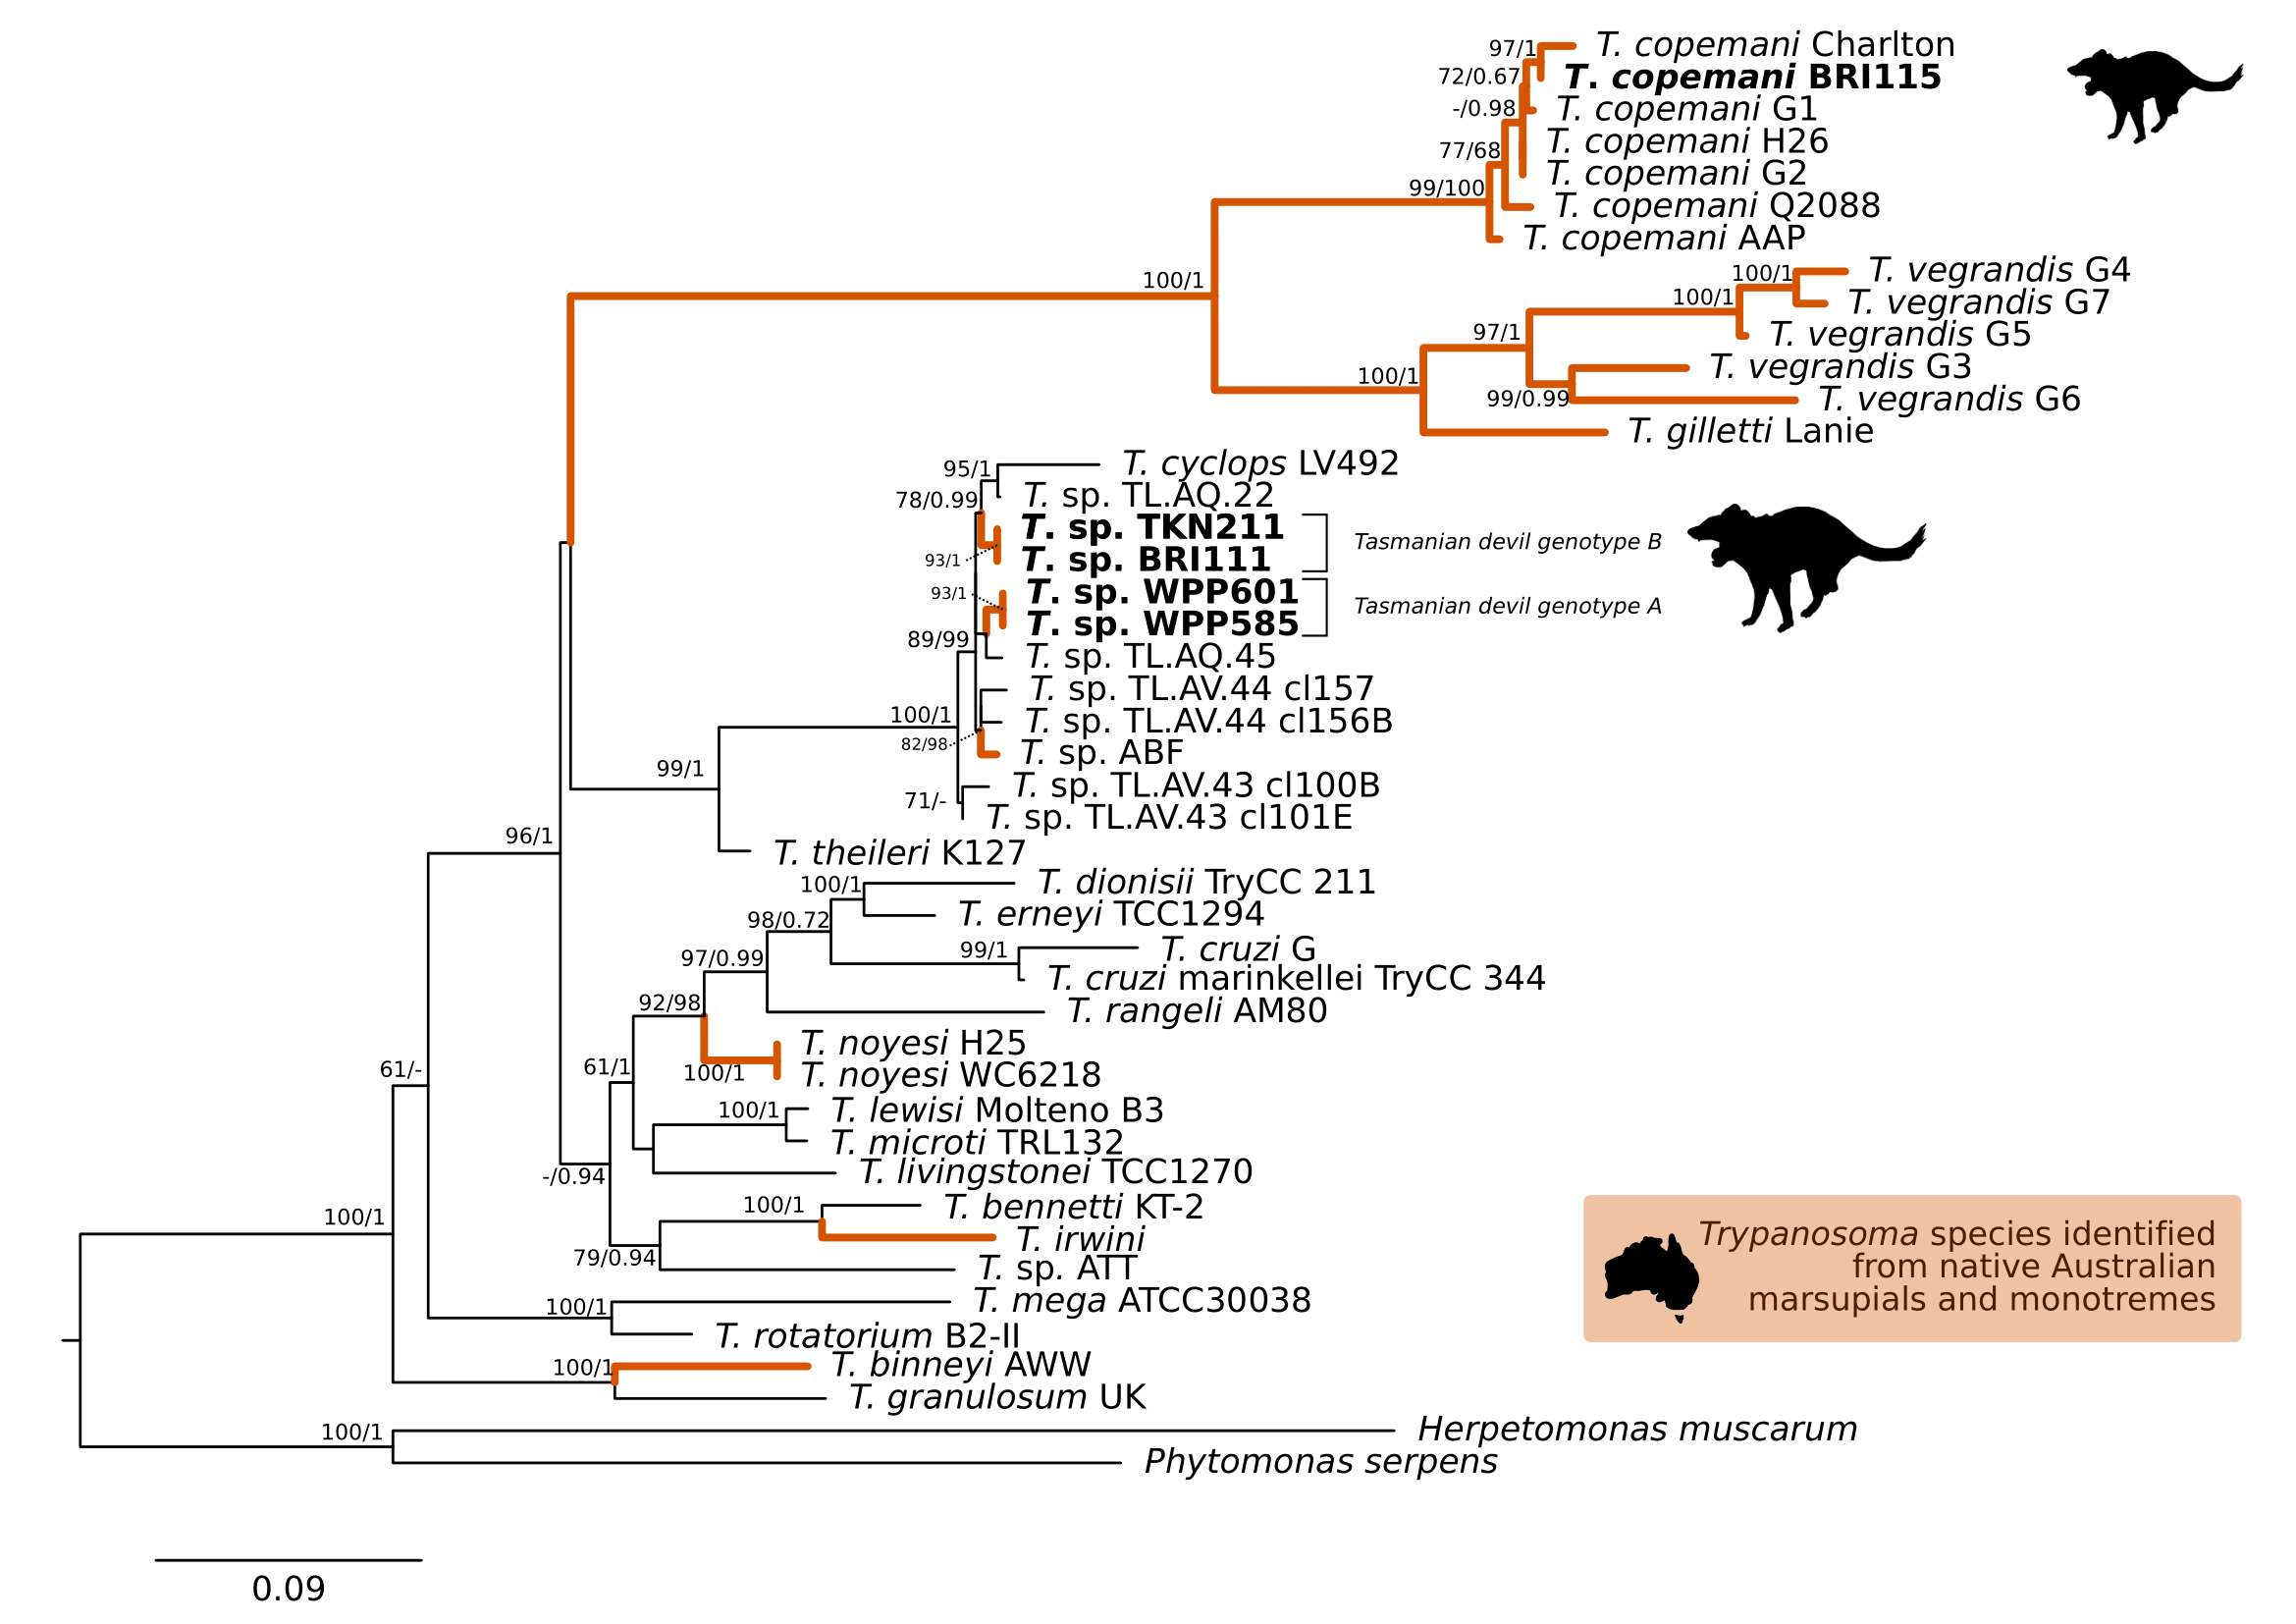
\includegraphics[width=0.95\linewidth]{figures/ms-figs/Ch6-Fig2} \caption[Phylogenetic tree (\textit{18S rRNA}) of \textit{Trypanosoma} spp. from the Tasmanian devil.]{Maximum likelihood (ML) phylogenetic reconstruction of the \textit{Trypanosoma} genus based on a 1,505 bp alignment of the 18S rRNA locus using TIM3e + I + G4 substitution model. Node values correspond to bootstrap support / aBayes support, values less than 60 are hidden. Number of substitutions per nucleotide position is represented by the scale bar. Lineages that have been described from native Australian marsupials are denoted by orange lines. Sequences generated in the present study in bold. GenBank accession numbers for sequences are available in Supplementary Table A.5.}\label{fig:F62}
\end{figure}

\begin{figure}
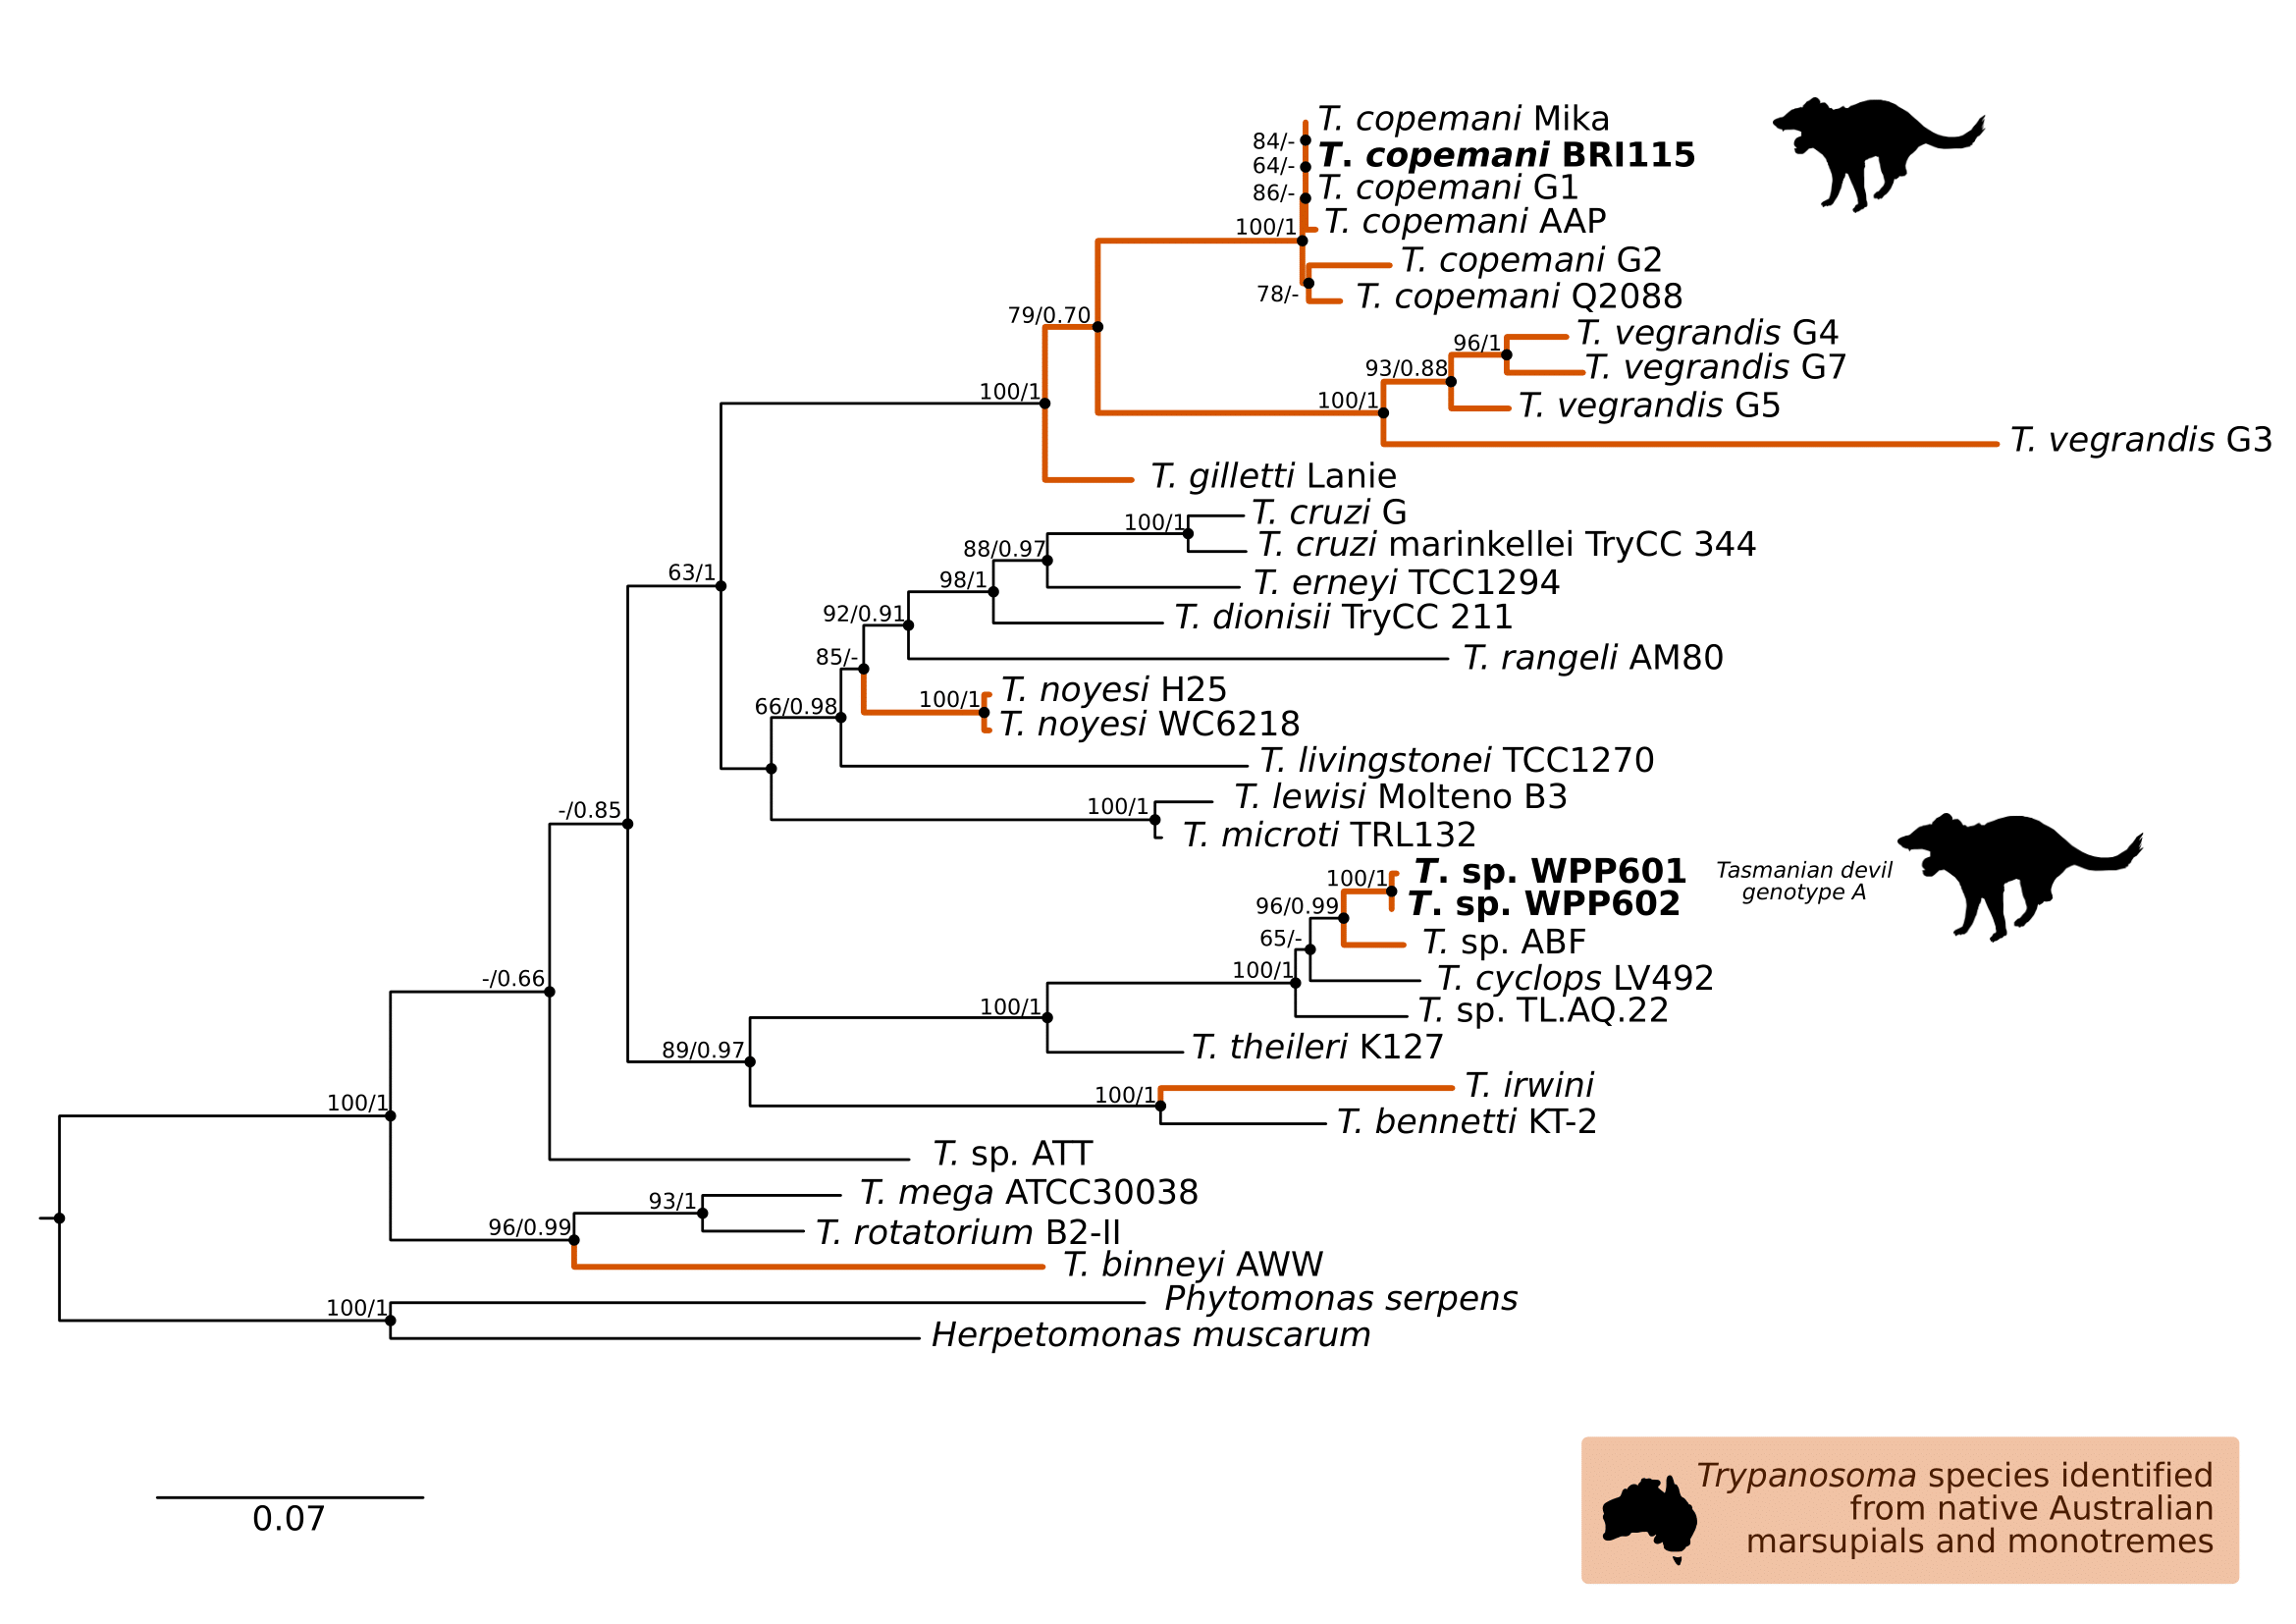
\includegraphics[width=0.95\linewidth]{figures/ms-figs/Ch6-Fig3} \caption[Phylogenetic tree (\textit{GAPDH}) of \textit{Trypanosoma} spp. from the Tasmanian devil.]{Maximum likelihood (ML) phylogenetic reconstruction of the \textit{Trypanosoma} genus based on a 767 bp alignment of glycosomal Glyceraldehyde Phosphate Dehydrogenase (\textit{gGAPDH}) using TN93 + F + I + G4 substitution model. Node values correspond to bootstrap support / aBayes support, values less than 60 are hidden. Number of substitutions per nucleotide position is represented by the scale bar. Lineages that have been described from native Australian marsupials are denoted by orange lines. Sequences generated in the present study in bold. GenBank accession numbers for sequences are available in Supplementary Table A.5.}\label{fig:F63}
\end{figure}

\begin{figure}
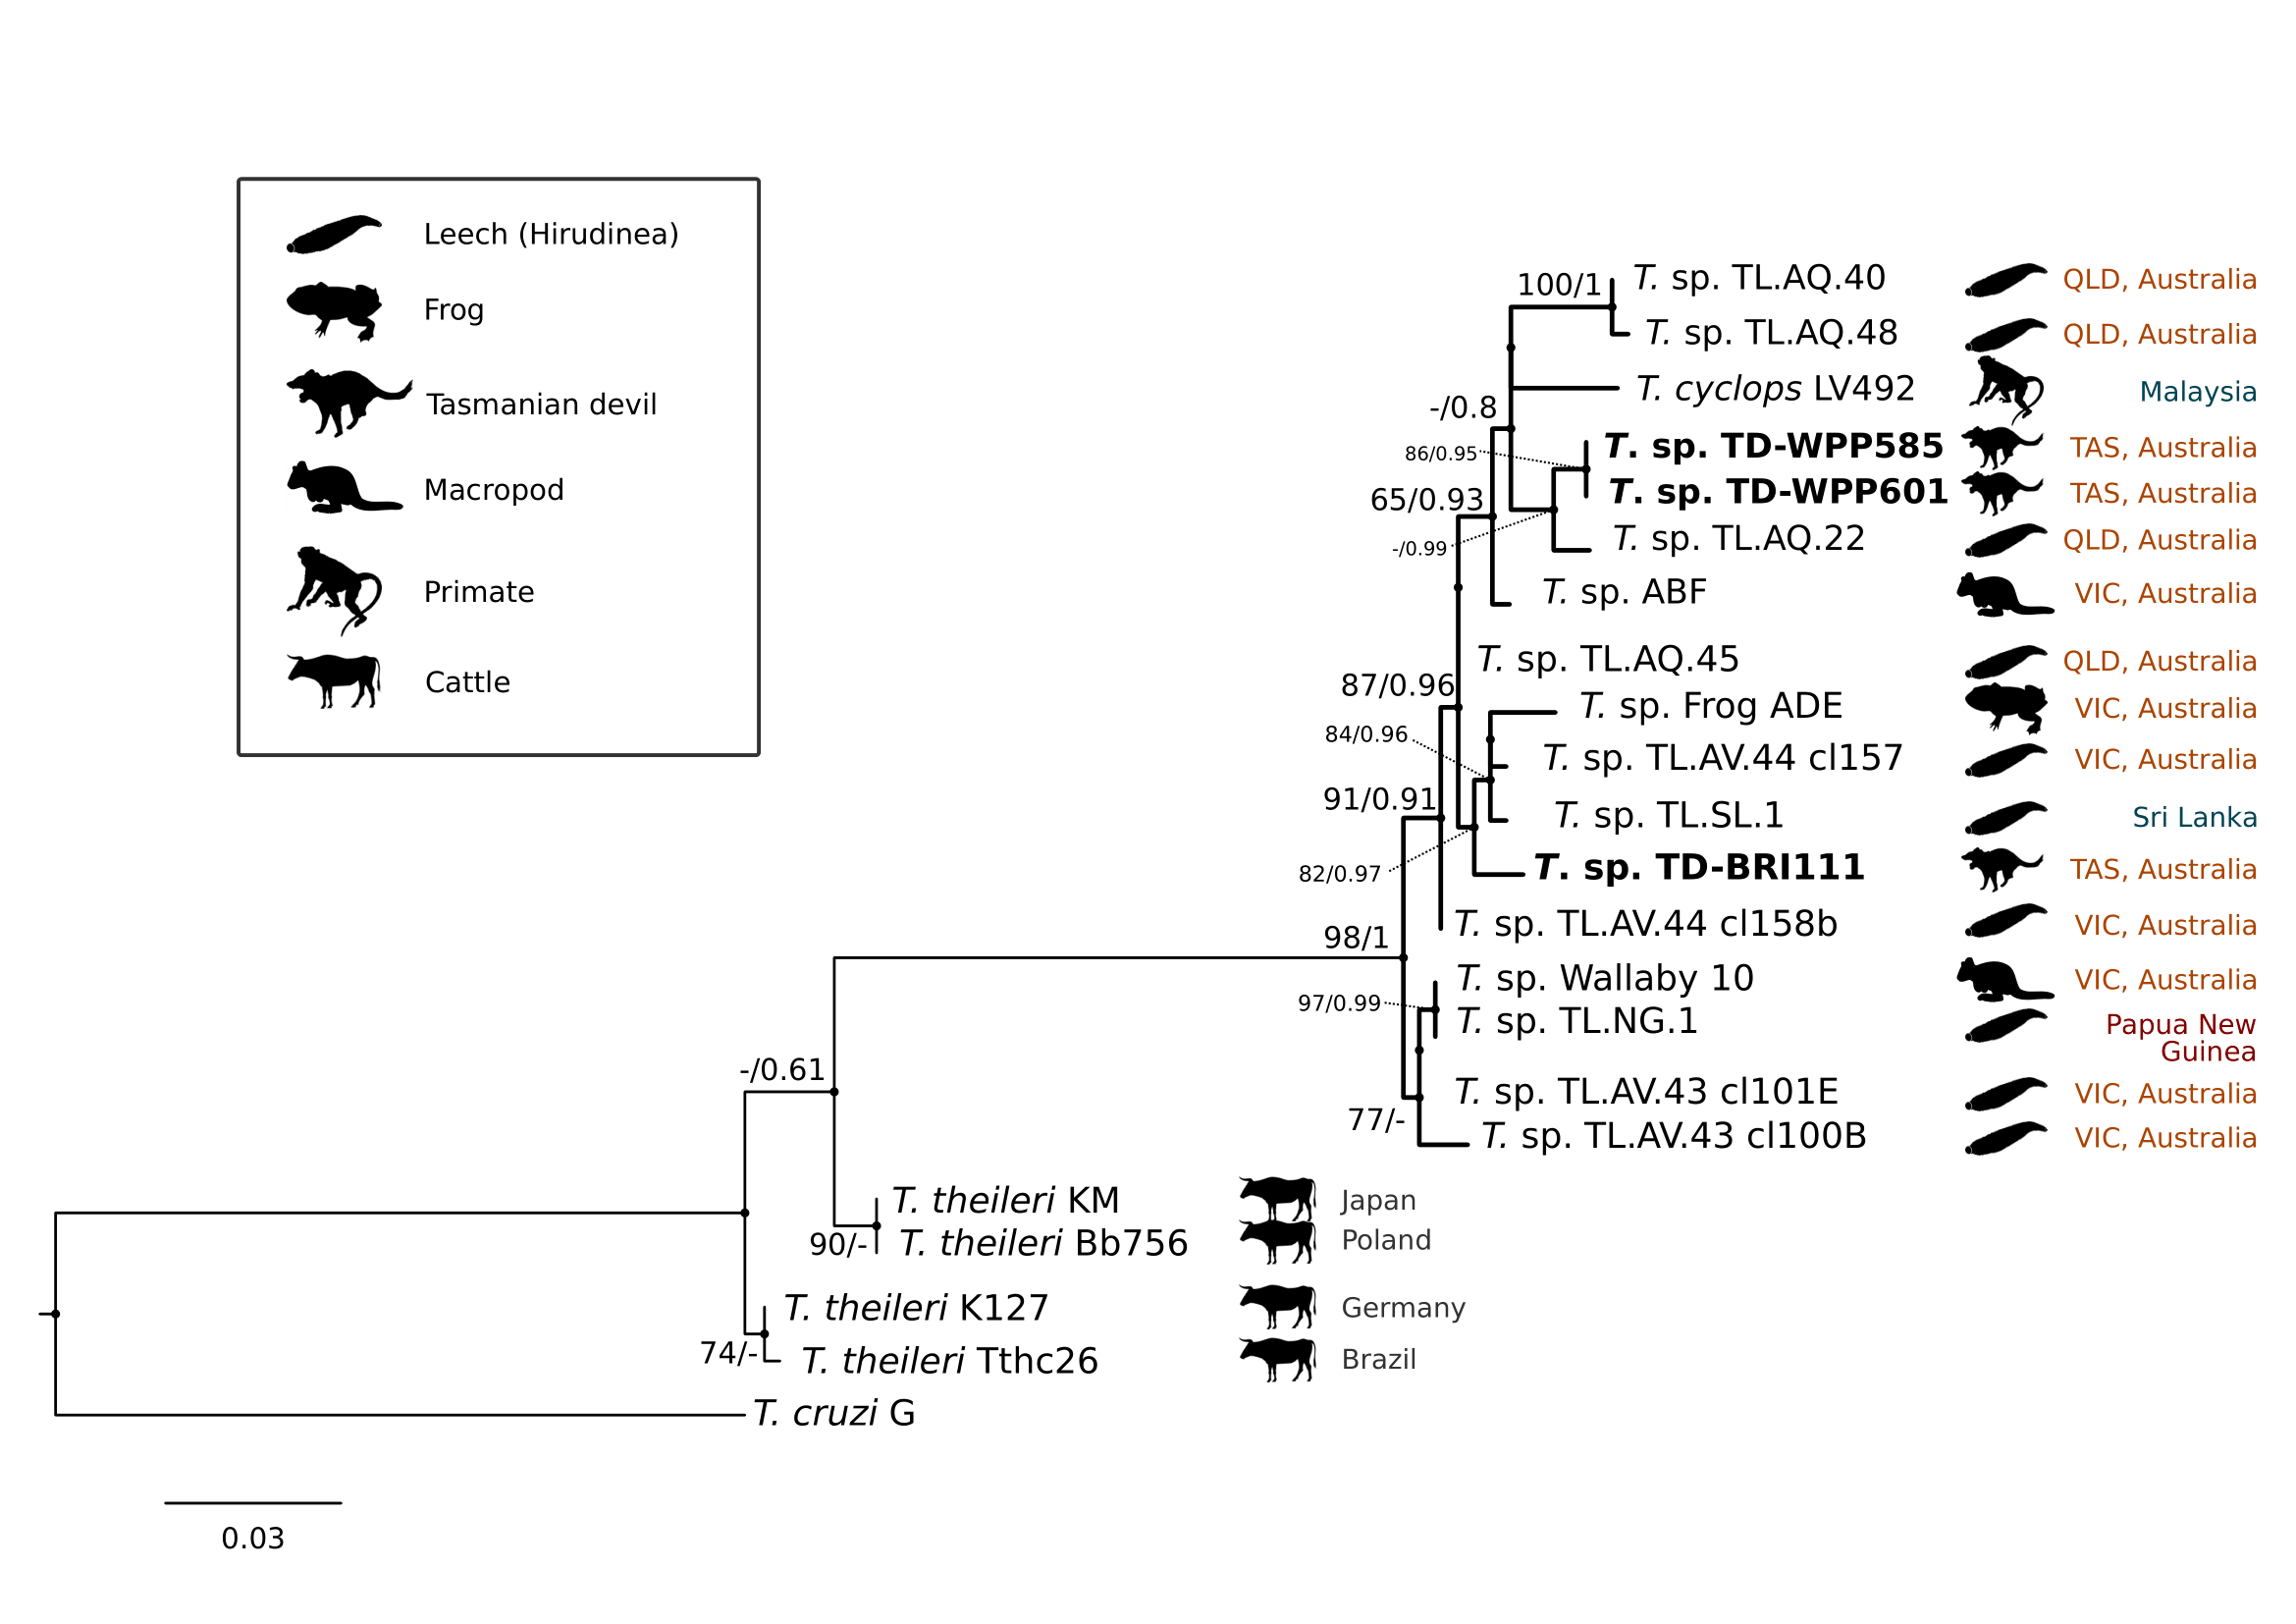
\includegraphics[width=0.95\linewidth]{figures/ms-figs/Ch6-Fig4} \caption[Phylogenetic tree of \textit{Tr. cyclops} clade (\textit{18S rRNA}, v7-8 region) from the Tasmanian devil.]{Maximum likelihood (ML) phylogenetic reconstruction of sequences from the \textit{Trypanosoma cyclops} clade based on a 559 bp alignment of the 18S rRNA locus across the V7-8 hypervariable region using K2P + G4 substitution model. Node values correspond to bootstrap support / aBayes support, values less than 60 are hidden. Number of substitutions per nucleotide position is represented by the scale bar. Australian states abbreviated to QLD (Queensland), TAS (Tasmania) and VIC (Victoria). GenBank accession numbers for sequences are available in Supplementary Table A.5.}\label{fig:F64}
\end{figure}

A single sample (BRI115) obtained from Black River site was positive for a \emph{Babesia} sp. and this individual was also positive for \emph{Tr. copemani} infection. Analysis of an 800 bp fragment of the 18S rRNA locus revealed it was similar to \emph{Babesia} sp. identified from \emph{Ixodes tasmani} in Queensland (MG251436; 96.0\% similarity) and \emph{Babesia lohae} from \emph{Ixodes holocyclus} in Queensland (MG593272; 95.5\% similarity).

\hypertarget{microscopy}{%
\subsection{Microscopy}\label{microscopy}}

Microscopy of blood smears from Takone site did not yield any positive detection of haemoparasites.

\hypertarget{discussion-2}{%
\section{Discussion}\label{discussion-2}}

The present study represents the first survey of haemoprotozoa from wild populations of the endangered Tasmanian devil. Our findings of \emph{Trypanosoma} infections across all four sites suggests that this infection is widespread and potentially endemic within Tasmanian devil populations. This wide distribution of \emph{Trypanosoma} across populations contrasts with the absence of \emph{Leishmania}, \emph{Theileria}, \emph{Hepatozoon}, or \emph{Plasmodium} species, and the low detection of \emph{Babesia} which was only detected in a single individual.

The extension of the host range of \emph{Tr. copemani} is notable and supports recent research identifying this parasite in a wide range of marsupial hosts from across Australia. To date, \emph{Tr. copemani} has been identified in all Australian states and territories except the Northern Territory and South Australia. The identification of this parasite in Tasmanian devils is potentially significant from a health perspective as previous reports have associated it with pathological changes in the woylie (\emph{Bettongia penicillata}) \autocite{boteroTrypanosomesGeneticDiversity2013,thompsonTemporalSpatialDynamics2014} and in koalas (\emph{Phascolarctos cinereus}) with co-morbidities \autocite{mcinnesPotentialImpactNative2011}. With this report, there are now at least ten Australian vertebrate host records for \emph{Tr. copemani}, therefore this \emph{Trypanosoma} species appears to be a marsupial generalist and capable of infecting a diverse range of mammals. Further studies to map the complete distribution and host range of \emph{Tr. copemani} will help provide insights into the co-evolution of this native trypanosome in its marsupial hosts.

The identification of genotypes from the \emph{Trypanosoma cyclops} clade was unexpected. \emph{Trypanosoma cyclops} was described from wild caught southern pig-tail macaques (\emph{Macaca nemestrina}) in jungle areas of West Malaysia \autocite{weinmanTrypanosomaCyclopsSp1972} and \textcite{hamiltonNewLineageTrypanosomes2005} identified novel genotypes of this clade from Australia, Papua New Guinea, and Sri Lanka. However, since its identification, there have been very few published reports of \emph{Tr. cyclops}. Phylogeny within the \emph{Tr. cyclops} clade was not well resolved, as demonstrated by the polytomy in Figure \ref{fig:F64}. The identification of two distinct genotypes in devils that do not form a monophyletic group, and show different level of relatedness to sequences overseas highlights the uncovered diversity within this clade. The closest named species to \emph{Tr. cyclops} is \emph{Trypanosoma} (\emph{Megatrypanum}) \emph{theileri}, which has a cosmopolitan distribution and predominantly infects cattle. The most important vector of \emph{Tr. theileri} is thought to be tabanid flies (Tabanidae) \autocite{hoareTrypanosomesMammalsZoological1972,werszkoMolecularDetectionMegatrypanum2020}. While this trypanosome is generally considered non-pathogenic, chronic infection has been associated with the development of secondary diseases in cattle \autocite{rodriguesCharacterizationSplicedLeader2010}.

The GAPDH gene has been shown to be a more suitable marker than the 18S rRNA locus for determining the phylogeny within the \emph{Trypanosoma} genus \autocite{hamiltonTrypanosomesAreMonophyletic2004}. A comparative analysis of \emph{Tr. copemani} shows intra-specific sequence similarity within the clade is 97.0--100\% and inter-specific similarity to the nearest named species, \emph{Tr. gilletti}, is 91.3--92.3\%. Intra-specific sequence similarity within the \emph{Tr. cyclops} clade was 94.8--99.9\%, while inter-specific sequence similarity to nearest named species, \emph{Tr. theileri}, is 90.4\%. Therefore, there is sufficient support that the sequences generated for devils can be attributed to \emph{Tr. cyclops}. Differentiation of genotypes within this clade are best identified by analysis of the V7--8 hypervariable region of the 18S rRNA locus (Figure \ref{fig:F64}, Table \ref{tab:TA62}). This study further supports that \emph{Tr. cyclops} is more closely related to sequences obtained from Australia, Papua New Guinea, and Sri Lanka than it is to \emph{Tr. theileri}. \autocite{hamiltonNewLineageTrypanosomes2005}. As shown in the phylogeny within the \emph{Tr. cyclops} clade (Figure \ref{fig:F64}) there is no geographical or host distinction between the different genotypes, further supporting the taxonomy as a single species. Research on functional traits including growth dynamics in culture coupled with morphological analysis is needed to better understand the taxonomy of this clade. The geographical and host extensions reported here will be useful for the future work aimed at understanding the evolutionary history of the \emph{Tr. cyclops} and \emph{Tr. theileri} clades and the \emph{Trypanosoma} genus more broadly \autocite{hamiltonEvolutionTrypanosomaCruzi2012}.

The description of a \emph{Tr. cyclops}-like species in this work expands the number of \emph{Trypanosoma} species in Tasmanian mammals to four. The platypus-specific \emph{Tr. binneyi} has been observed from blood samples and subsequently described phylogenetically \autocite{mackerrasHaematozoaAustralianMammals1959,jakesPhylogeneticRelationshipsTrypanosoma2001,papariniNovelGenotypesTrypanosoma2014} with suggestions that leeches are the likely vector \autocite{papariniNovelGenotypesTrypanosoma2014}. Trypanosomes have also been identified in populations of the eastern barred bandicoot (\emph{Perameles gunnii}) and southern brown bandicoot (\emph{Isoodon obesulus}) \autocite{bettiolFirstRecordTrypanosomes1998}, however due to well-described limitations of morphological identification \autocite{lukesEvolutionParasitismKinetoplastid2014}, species-level identification has not been achieved. Additionally, \emph{Tr. copemani} was identified for the first time in Tasmania in 2020 from wild populations of the eastern quoll (\emph{Dasyurus viverrinus}) \autocite{portasBaselineHealthDisease2020}. The current study now brings the number of known trypanosome hosts in Tasmania to five, with the addition of Tasmanian devils, and confirmation of a new species from the \emph{Tr. cyclops} clade. It is interesting to note that while previous studies have described only one species of \emph{Trypanosoma} in the sampled hosts from Tasmania, in the current study we have described at least two species circulating in devils. The higher diversity of \emph{Trypanosoma} species found in devils might be a consequence of our larger sample size or spatial coverage in comparison to previous studies.

Despite molecular identification of \emph{Trypanosoma} infection in devils from Takone, no trypomastigotes were observed in corresponding blood smears. This finding is consistent with other studies which have found molecular tools are more sensitive than microscopy for trypanosome detection \autocite{paguemWidespreadCoendemicityTrypanosoma2019,rodriguesUncoveringTrypanosomaSpp2019}. The absence of patent parasitaemia (i.e.~no flagellates observed in fresh blood smears) could be the result of low-level infections; however it may also indicate that devils are not a competent host of the \emph{Trypanosoma} species \autocite{brandaoTrypanosomatidsSmallMammals2019}.

The trypanosomatids are obligatory parasites with a single flagellum and include several genera that are pathogenic to humans, animals and plants \autocite{davila-levyExploringEnvironmentalDiversity2015,maslovRecentAdvancesTrypanosomatid2019}. Due to their medical importance, trypanosomatids have been studied more intensively with trypanosome and \emph{Leishmania} parasites the causative agents of sleeping sickness (\emph{Trypanosoma brucei gambiense} and \emph{Trypanosoma brucei rhodesiense}), Chagas disease (\emph{Trypanosoma cruzi}) and leishmaniases \autocite{davila-levyExploringEnvironmentalDiversity2015,lukesTrypanosomatidsAreMuch2018}. Broadly, \emph{Trypanosoma} species can be divided into two groups based on their transmission route; the salivarian trypanosomes which are transmitted via the saliva of the tsetse fly (\emph{Glossina} spp.), and stercorarian trypanosomes which are passed to their host via the faeces of the arthropod intermediate host \autocite{jacksonGenomeEvolutionTrypanosomatid2015}. The vectors of Australian trypanosomes are still largely unknown, with few studies investigating the presence of trypanosomes in invertebrates. Previous studies have implicated ticks (\emph{Ixodes} spp.) \autocite{mackerrasHaematozoaAustralianMammals1959,austenVectorTrypanosomaCopemani2011} and tabanid flies \autocite{boteroMorphologicalPhylogeneticDescription2016} as potential vectors. While it has been hypothesised that carnivory is important in the maintenance of trypanosomes, experimental studies do not support this \autocite{roelligOralTransmissionTrypanosoma2009}, and instead suggested that increased infection is attributed to insectivores who consume infected arthropod vectors \autocite{rochaTrypanosomaCruziInfection2013}. The phylogenetic position of the \emph{Tr. cyclops} clade within the stercorarian group means that its potential vector(s), could be a range of arthropod(s) with transmission occurring via contact with vector faeces. It is interesting however that although members of this clade have been identified from leeches and frogs \autocite{hamiltonNewLineageTrypanosomes2005}, their phylogenetic position is distinct from other aquatic and leech-associated \emph{Trypanosoma} species \autocite{hamiltonTrypanosomesAreMonophyletic2004,hamiltonPatternsCoevolutionTrypanosomes2007,papariniNovelGenotypesTrypanosoma2014,lemosPhylogeneticMorphologicalCharacterization2015}. The range extensions of both \emph{Tr. copemani} and \emph{Tr. cyclops} clades recorded in the present study provide additional data to aid vector identification. The large geographical range of both these \emph{Trypanosoma} species suggests that any vector(s) should be equally ubiquitous and capable of biting or coming into close contact with a wide range of vertebrate hosts.

In the present study, we validated that a previously published \emph{Trypanosoma} PCR assay \autocite{mcinnesTrypanosomaIrwiniSp2009} is also capable of detecting/amplifying \emph{Leishmania} DNA. Two controls of genetically diverse species of \emph{Leishmania}, \emph{L. infantum} and \emph{L. macropodum}, \autocite{barrattIsolationNovelTrypanosomatid2017} were used. In the context of this study, we determined that generic trypanosome primers are able to amplify \emph{L. macropodum}, which was identified as a cause of cutaneous leishmaniasis in kangaroos \autocite{roseCutaneousLeishmaniasisRed2004}. The preferred diagnostic sample for the detection of \emph{Leishmania} is generally bone marrow aspirate or tissue samples, however previous studies have recorded detection via blood samples \autocite{humbergLeishmaniaChagasiOpossums2012,medkourCanineVectorborneProtozoa2020}. Obtaining bone marrow and internal tissue samples from free ranging wildlife is not practical or ethical, especially where populations are experiencing significant declines. While the present study reported the absence of \emph{Leishmania} via PCR of blood samples, it is not possible to discount occult infection and future studies utilising additional sample types would be recommended. Although co-infections of \emph{Leishmania} and \emph{Trypanosoma} cannot be ruled out completely in the individuals tested here, the absence of \emph{Leishmania} DNA is consistent with previous studies that have utilised the same assay on other Australian mammals \autocite{papariniIdentificationNovelTrypanosome2011,austenInvestigationMorphologicalDiversity2015,barbosaSequenceAnalysesMitochondrial2019}. Therefore, reports of Australia's only endemic \emph{Leishmania} species remain confined to kangaroos and biting midges (Ceratopogonidae) in the Northern Territory \autocite{roseCutaneousLeishmaniasisRed2004,dougallNewReportsAustralian2009,dougallEvidenceIncriminatingMidges2011}.

An unexpected outcome was the low detection of \emph{Babesia} species and the lack of detection of \emph{Theileria} and \emph{Hepatozoon} species.
Recent molecular studies in Australian wildlife have demonstrated a range of unique endemic piroplasms, with reports of up to 80--90\% prevalence in some marsupial host populations \autocite{rongHighPrevalenceTheileria2012,papariniFirstMolecularCharacterization2015,northoverIncreasedTrypanosomaSpp2019}.
Piroplasms and \emph{Hepatozoon} spp. are transmitted by ticks and therefore dependent on the density and interactions between host and vector(s) to continue their lifecycle.
Recent investigations have revealed the presence of numerous novel \emph{Babesia}, \emph{Theileria} and \emph{Hepatozoon} species in native Australian ticks \autocite{greayEndemicExoticNovel2018,lohMolecularSurveillancePiroplasms2018,storey-lewisMolecularDetectionCharacterisation2018}.
With respect to the single identification of \emph{Babesia} at the Black River site, the genetic relationship shows it is most closely related to \emph{Babesia lohae} sequences identified in \emph{Ixodes holocyclus} and \emph{Ixodes tasmani} ticks from the east coast of Queensland \autocite{greayEndemicExoticNovel2018,lohMolecularSurveillancePiroplasms2018}.
The low prevalence of \emph{Babesia} might be attributed to seasonality of tick infestations, as has been described in relationship between \emph{Ix. tasmani} ticks and brushtail possums hosts \autocite{murdochEcologyCommonMarsupial2005}.
Future longitudinal sampling including multiple seasons are valuable to better understand the phylogeny and epidemiology of this \emph{Babesia} species circulating in devil populations.

In Tasmania, piroplasms and \emph{Hepatozoon} species have been identified from three marsupial species and more recently from ticks (\emph{Ixodes} spp.). A \emph{Hepatozoon} has been identified in eastern barred bandicoots (\emph{Perameles gunnii}) \autocite{bettiolFirstRecordMember1996} by morphological examination of blood smears and the eastern quoll (\emph{Dasyurus viverrinus}) through molecular tools \autocite{portasBaselineHealthDisease2020}. \emph{Theileria} species have been identified from eastern bettongs (\emph{Bettongia gaimardi}) \autocite{portasHealthEvaluationFreeranging2014} and eastern quolls \autocite{portasBaselineHealthDisease2020}. A molecular survey of ticks (\emph{Ix. tasmani}) from Tasmanian devils demonstrated 34.1\% (15/44) of sample pools were positive for \emph{Hepatozoon} sp. \autocite{vilcinsDetectionHepatozoonSpotted2009}. More recently, novel species of \emph{Theileria} and \emph{Hepatozoon} were identified from \emph{Ix. tasmani} collected in Tasmania \autocite{greayEndemicExoticNovel2018,lohMolecularSurveillancePiroplasms2018}. Given the high prevalence of \emph{Ix. tasmani} parasitising sampled Tasmanian devils (Ruiz-Aravena pers. comms.), the low prevalence of piroplasms and \emph{Hepatozoon} species is therefore unexpected. This raises important questions about the sylvatic lifecycle and reservoir hosts of these piroplasm and \emph{Hepatozoon} species, suggesting potential and contrasting explanations: (i) Tasmanian devils are not competent reservoir hosts or (ii) they are natural hosts which are able to mount a sufficient immune response against the infection. In both cases, parasitaemia might be low or absent. Additional explanations could include (iii) infections by haemoprotozoa are acute and fatal to Tasmanian devils, however the absence of \emph{Theileria} and \emph{Hepatozoon} in DFTD-free individuals makes this hypothesis less likely; or (iv) the detection of haemoprotozoa in ticks is an opportunistic/accidental finding and they are not competent vectors of these organisms. Additional sampling from DFTD-free populations and capturing seasonal variation will be important to assess the prevalence and susceptibility of Tasmanian devils to these haemoprotozoans.

The inclusion of morphological data obtained from blood smears and the application of additional molecular tools, such as \hl{high-throughput sequencing} to identify co-infections \autocite{barbosaIncreasedGeneticDiversity2017} and genome level information \autocite{reis-cunhaWholeGenomeSequencing2018}, are vital for further work. The collection of additional tissue samples may also prove useful for developing diagnostic tools, as well as better understanding the lifecycle of haemoprotozoa in the host. For example, bone marrow, skeletal muscle, tongue, brain and liver samples have been tested positive for \emph{Trypanosoma} DNA, while blood (including blood smears) were negative \autocite{northoverDebilitatingDiseasePolyparasitised2018}. While there is a body of work demonstrating Australian mammals are hosts to a range of endemic species of \emph{Trypanosoma}, \emph{Leishmania}, \emph{Babesia}, \emph{Theileria} and \emph{Hepatozoon} \autocite{austenInvestigationMorphologicalDiversity2015,boteroMorphologicalPhylogeneticDescription2016,barbosaSequenceAnalysesMitochondrial2019,northoverIncreasedTrypanosomaSpp2019}, the clinical impact of these haemoprotozoa is largely unknown. This is particularly important in the context of endangered species such as the Tasmanian devil.

The results presented here highlight the need for additional studies on the haemoprotozoa and broader parasite community of Tasmanian devils. In order to provide meaningful information for management and conservation strategies, it is vital that the complete biology of this species be understood. Conservation strategies including translocation, captive breeding and establishment of insurance populations are management strategies that have been implemented in the case of Tasmanian devils. Parasite communities are an important consideration in species recovery, highlighting the need to further study host-parasite relationships \autocite{northoverHiddenConsequencesAltering2018}. For example, while translocation of animals could facilitate introduction of parasites into new host populations, the same translocation could dilute adaptations of the receiving populations to the local parasites. This last case is particularly relevant when the local individuals in supplemented populations are outnumbered by the translocated individuals. Immediate future work is now needed to document the prevalence and diversity of haemoprotozoa in devils with a focus towards understanding the clinical impacts of infection and importantly impact of co-infection with DFTD.

\hypertarget{conclusion-1}{%
\section{Conclusion}\label{conclusion-1}}

Here, we have provided the first insights into haemoprotozoa infecting the endangered Tasmanian devil. Further research is urgently needed to document the full haemoprotozoan diversity in the Tasmanian devil, with a focus towards understanding the clinical significance of these infections and co-infections with DFTD. The identification of \emph{Tr. copemani} and novel members of the \emph{Tr. cyclops} clade provide further insights into the co-evolution of trypanosomes in marsupials, showing Australian native fauna harbour genetically unique parasitic species. Finally, the lack of detection of major haemoprotozoa genera; \emph{Hepatozoon}, \emph{Leishmania}, \emph{Plasmodium} and \emph{Theileria} in our study opens questions about the overall status of these parasites in the island ecosystem of Tasmania and whether their absence might reflect specific host-parasite interactions.

\hypertarget{gendiscussion}{%
\chapter{Discussion}\label{gendiscussion}}

\hypertarget{synthesis-of-key-findings-in-thesis-chapters}{%
\section{Synthesis of key findings in thesis chapters}\label{synthesis-of-key-findings-in-thesis-chapters}}

The main aims of this thesis were to understand the diversity of ticks parasitising urban wildlife and to characterise the microbial communities associated with these ticks and their wildlife hosts.
To address the aims, this thesis was divided into three major themes: (1) Australian ticks, (2) bacteria and haemoprotozoa present in wildlife and ticks, and (3) molecular characterisation of microbes.

This thesis has provided insights into the tick fauna present in Australia, particularly at the urban fringe which is a high-risk area for potential spillover events \autocite{plowrightLandUseinducedSpillover2021}.
Zoonotic spillover events occur when pathogens jump from animals to humans; over 70\% of these spillover events have originated in wildlife \autocite{jonesGlobalTrendsEmerging2008}.
The public health significance of spillover events has never been more relevant than at the time of writing this thesis.
The COVID-19 pandemic caused by the SARS-CoV-2 virus \autocite{luGenomicCharacterisationEpidemiology2020a}, has brought to the forefront the fragility of current human society and the devastating health and financial consequences these emerging pathogens have.
Additionally in 2020, the exotic canine tick-borne disease canine monocytic ehrlichosis, caused by the \emph{Ehrlichia canis}, was identified in Australian dogs; and has been identified in dogs from Western Australia, Northern Territory and South Australia\footnote{\url{https://www.outbreak.gov.au/current-responses-to-outbreaks/ehrlichiosis-dogs}}.

In Chapter \ref{austicks} the low diversity of tick species within the Australian environments examined was highlighted.
A review of human tick bites in Australia is also included in Chapter \ref{austicks}, and this informed the subsequent focus on: the Australian paralysis tick \emph{Ixodes holocyclus} and the ornate kangaroo tick \emph{Amblyomma triguttatum}.
Chapter \ref{austicks} described a high-throughput tool kit to identify ticks and the development of barcode sequences which can be used as references to identify Australian ticks.

Chapters \ref{wildlife-bacteria} and \ref{wildlife-haemoprotozoa} described the bacterial and haemoprotozoal communities in wildlife and their ticks.
In these chapters, molecular tools were used to investigate potential agents of tick-borne disease that are present in wildlife.
These chapters identified that the bacterial and haemoprotzoal organisms present were mostly unique between wildlife species, and there was little overlap between microbes present in ticks and host blood and tissue samples.
The main exception to this finding was the \emph{Anaplasmataceae} family.
To the best of my knowledge, Chapter \ref{wildlife-bacteria} represents the first report of \emph{Neoehrlichia} and \emph{Ehrlichia} from Australian wildlife (blood and/or tissue samples).
In this bacterial family, \emph{Neoehrlichia} was more prevalent in blood samples from hosts than ticks but was identified in tick species that are known to bite humans, including \emph{Ix. holocyclus}.
At Sydney sites, `\emph{Ca}. Neoehrlichia arcana' was readily identified in black rats and long-nosed bandicoots.
At Perth study sites, a novel species of \emph{Ehrlichia} from chuditch blood was identified. Common `taxa of interest' shared between samples from the west and east coast were not identified.
Therefore, from the results generated in this thesis, it suggests that human tick-borne pathogens, if any, are likely to be different between these areas of Australia due to differences in bacteria identified as a consequences of tick species and vertebrate hosts.

In Chapters \ref{black-rat} and \ref{tas-devil}, haemoprotozoa in Australian wildlife were further investigated.
\emph{Trypanosoma lewisi}-like sequences were identified in the blood of black rats in Sydney, New South Wales.
As this trypanosome has been implicated in the extinction of rodents in some localities \autocite{wyattHistoricalMammalExtinction2008}, further genetic information was obtained to provide insight into the phylogeny of this species.
Analysis revealed the sequences were distinct from the \emph{Tr. lewisi} sensu stricto clade and were most closely related to genotypes from Europe.
Chapter \ref{tas-devil} was the result of a collaborative research project with the University of Tasmania and provided molecular insights into blood parasites from the Tasmanian devil.
Within the broader context of this thesis, this research is also of interest for zoonotic disease surveillance.
As a large carnivore, devils fill a unique ecological niche and these findings add further information about the identification of unique parasites from Australian wildlife.

\hypertarget{a-one-health-approach}{%
\section{A One Health approach}\label{a-one-health-approach}}

As the importance of a One Health approach gains increasing attention globally, the implementation of policy and programs still proves challenging \autocite{predictconsortiumImplementingOneHealth2020}.
Development of national platforms and policies which facilitate coordination and integration of activities and programs across sectors is required.

\hypertarget{australian-programs}{%
\subsection{Australian Programs}\label{australian-programs}}

On a national level in Australia there is a One Health program that focuses on a number of subjects, including zoonoses, in the Indo-Pacific region\footnote{\url{https://aciar.gov.au/one-health}}. This program is a joint initiative through the Australian Centre for International Agriculture (ACIAR) and the Department of Foreign Affairs and Trade (DFAT).
The Australian Centre for Disease Preparedness (ACDP), formerly known as the Australian Animal Health Laboratory is run by the Commonwealth Scientific and Industrial Research Organisation (CSIRO). Its aim is to protect Australia's livestock and aquaculture industries, and the general public, from emerging infectious disease threats. All state and territories in Australia also have government bodies relating to health and agriculture.
Wildlife Health Australia is a non-government organisation (NGO) that operates on a national level.
It has a strong One Health focus and provides a platform to link the environment, animal health and public health sectors, across government and non-government organisations\footnote{\url{https://wildlifehealthaustralia.com.au}}.

These organisations coordinate important programs, however, there is still much room for improvement in regard to surveillance programs in Australia \autocite{woodsImportanceWildlifeDisease2019}.
In most cases surveillance programs run by these organisations are centred around diseases of economic importance (e.g.~transmissible spongiform encephalopathy (TSE) Freedom Assurance Project\footnote{\url{https://www.animalhealthaustralia.com.au/what-we-do/disease-surveillance/tse-freedom-assurance-program/}}) or the identification of known pathogens (e.g.~arbovirus surveillance program\footnote{\url{https://ww2.health.wa.gov.au/Articles/A_E/Arbovirus-surveillance-program}}).
As has been shown by the growing body of evidence over the last five years, and from the results presented in this thesis, it is most likely that any agent(s) of human tick-borne disease in Australia are likely novel and currently unrecognised.
Techniques that are able to identify a broad range of microbes need to be used in these surveillance programs.
The practical implementation of this is difficult for logistical and financial reasons.
As a result, research into novel microbes is generally carried out in the university sector in Australia.
Funding for research by university academics is highly competitive, and most often these researchers do not have access to government and NGO infrastructure or networks for conducting surveillance and monitoring programs on the ground.
Cooperation between university and government sectors would improve technical support and research methodology for all parties, ensuring a robust surveillance program, with efficient use of resources and expertise.

\hypertarget{value-of-notifiable-disease-inclusion}{%
\subsection{Value of notifiable disease inclusion}\label{value-of-notifiable-disease-inclusion}}

The Australian National Notifiable Diseases Surveillance System (established 1990) co-ordinates the surveillance on an agreed list of communicable diseases and disease groups in Australia.
The list includes a number of mosquito-borne viruses and some tick-associated diseases such as Q-fever \hl{(\emph{Coxiella burnetii})} and tularaemia (\emph{Francisella tularensis}) \footnote{\url{https://www1.health.gov.au/internet/main/publishing.nsf/Content/cda-surveil-nndss-casedefs-distype.htm}}.
There are a number of tick (and vector) associated agents that are not included in this list, including \emph{Babesia}, \emph{Borrelia}, \emph{Bartonella}, and \emph{Rickettsia} spp.
State and territory jurisdictions have an expanded list of notifiable diseases, where some of the infectious agents mentioned above are included.
For example, in Western Australia, \emph{Rickettsia} infection (including spotted fevers and all forms of typhus fever) is notifiable \footnote{\url{https://ww2.health.wa.gov.au/Articles/N_R/Rickettsia-typhus-and-others}}.
Notifiable diseases are accompanied by a clear case definition and requirements for reporting (e.g.~inclusion of confirmed and suspected cases).
The geographical location where infection occurred (acquired overseas or locally) does not influence the requirement to provide notification of a case.
Once infectious agents (or putative pathogens) have been identified, their inclusions on the list of nationally notifiable diseases will be a useful step towards obtaining a clearer picture of the impact of tick-borne diseases in Australia.

The incorporation of human case data adds another layer to wildlife surveillance studies.
This type of holistic approach to understanding disease dynamics has started to provide important insights into Australian mosquito borne diseases \autocite{ongMosquitoBorneVirusesNonHuman2021}.
For example, a study of 31 species of nonhuman vertebrates in southeast Queensland found that seropositivity of Ross river virus (alphavirus, \emph{Togaviridae} family) was highly correlated with human notification data \autocite{skinnerSpeciesTraitsHotspots2020}.
A similar approach with the causative agent of human buruli ulcer (\emph{Mycobacterium ulcerans}), has shown that there was a high geographical correlation between human cases of this disease and the positive identification of the bacteria in possum faecal samples \autocite{carsonPotentialWildlifeSentinels2014}.
Thus, a central recording system of tick-borne infection in Australia will be a useful step towards obtaining a better understanding of the impact and distribution of disease.

\hypertarget{unique-microbes-at-the-urban-wildlife-interface-in-australia}{%
\section{\texorpdfstring{\hl{Unique microbes at the urban-wildlife interface in Australia}}{Unique microbes at the urban-wildlife interface in Australia}}\label{unique-microbes-at-the-urban-wildlife-interface-in-australia}}

\hl{The local emergence of vector-borne diseases is driven by human factors which then enhance enzootic cycles; in contrast, pathogen invasion results from anthropogenic movements (such as trade and travel) where conditions (such as host(s), vector(s), and climate) are suitable for a pathogen \autocite{kilpatrickDriversDynamicsControl2012}.}
\hl{Current surveillance of infectious diseases generally targets threats to human and livestock health.Research conducted in this thesis provides further supports for the growing body of evidence that there is an absence of known Northern hemisphere tick-borne pathogens in Australia. There have now been several studies using molecular tools (including both targeted and generic assays) demonstrating that Australian ticks and wildlife harbour a unique diversity of microbes, and not any of the recognised pathogens referred to above \autocite{goftonBacterialProfilingReveals2015,eganBacterialCommunityProfiling2020,hussain-yusufScreeningRickettsiaCoxiella2020}. This thesis demonstrates that the additional inclusion of wildlife health is important for surveillance programs.}

In particular, there has been little recent research on the potentially zoonotic pathogens of the invasive black rat in Australia \autocite{banksReviewEvidencePotential2012}.
The present thesis identified a number of novel microbes from black rats and reported new host records.
For example, a novel \emph{Borrelia} sp. was identified from tissue samples in Sydney.
Phylogenetic analysis showed this genotype formed a distinct clade with other rodent-associated sequences reported from Spain and United States of America.
It was interesting that this species was not identified in any of the ticks that were collected at the same time, which indicates that transmission may involve another vector or route.
The main vectors of the relapsing fever \emph{Borrelia} group are the soft ticks (family Argasidae), while \emph{Borrelia recurrentis} is transmitted by the human body louse \hl{(\emph{Pediculus humanus humanus})} \autocite{gilIdentificationNewBorrelia2005}.
Possible vectors of the rodent associated \emph{Borrelia} clade may include fleas, chiggers, mites, and lice.
\hl{The unique \emph{Borrelia} identified from rodents raises a number of questions, given that it is widespread in the northern hemisphere. Firstly, the large geographical distribution of this clade is striking. Presently, the clade appears to be rodent-specific, and the vector and pathogenicity are not known}.

The long-nosed bandicoot and black rat had similarities with regard to their tick fauna, and bacterial and haemoprotozoal taxa of interest.
Results in Chapters \ref{wildlife-bacteria} and \ref{wildlife-haemoprotozoa} identified \emph{Ix. holocyclus}, \emph{Ix. tasmani} and \emph{Ix. trichosuri} ticks on both hosts.
In Chapter \ref{wildlife-bacteria} \emph{Neoehrlichia} spp. were identified from both hosts and Chapter \ref{wildlife-haemoprotozoa} identified overlap with species of \emph{Theileria} and \emph{Trypanosoma}.
Overall, the arboreal hosts, possums and chuditch, exhibited differences in the microbes and `taxa of interest' identified, compared to the non-arboreal hosts.
The separation of hosts by ecological niche (i.e.~arboreal vs non-arboreal) is an interesting finding.
Although the sampling bias and relatively low numbers in the present thesis limit statistical inferences, it does provide support that future studies should explore this relationship in a systematic way.
For example, dual trapping regimes at sites which target (i) small, ground dwelling animals and (ii) small-medium sized semi-arboreal/arboreal animals may help overcome this sampling bias.

Recent research in Australia has provided insights into the relationship between ticks and local invasive animals, such as black rats and rabbits \autocite{lydeckerPeriurbanBlackRats2019,taylorInvasiveRabbitsHost2020}.
For example, the prevalence of zoonotic pathogens in mice and rats overseas has been reported to vary markedly over short geographical distances \autocite{rothenburgerEnvironmentalFactorsZoonotic2017}.
In the present study, there was a higher diversity of `taxa of interest' in black rats than native animals.
Attempts to understand the movement and establishment of pathogens or microbes between vertebrate hosts are difficult in the urban landscape.
The adaptation of black rats to urban life, means that this species should actually be regarded as a native species (or commensal) of urban landscapes \autocite{banksEcologicalImpactsCommensal2015}.
In other words it is the native wildlife that are invasive when they encroach on urban areas.
Where there are long periods of co-habitation between vertebrate species, it can make it difficult to understand the true movement of pathogens and untangle the dynamics of spillover events.
In the case of the \emph{Tr. lewisi}-like sequences reported in Chapters \ref{wildlife-haemoprotozoa} and \ref{black-rat}, it is most likely that spillover of this protozoan occurred from black rats to native rodents, however the timing and impact of this event(s) are unclear.
\hl{It is noted from a zoonotic perspective that \emph{Tr. lewisi} infection is rarely reported. While the first report of human infection was recorded in Thailand \autocite{sarataphanDiagnosisTrypanosomaLewisilike2007}, there is no evidence to suggest it is a widespread cause of trypanosomiasis}.
The movement of \emph{Theileria} cf.~\emph{peramelis} identified in Chapter \ref{wildlife-haemoprotozoa} is most likely to have occurred from long-nosed bandicoots into black rats.
This is due to the phylogenetic position of the parasite species within the native marsupial \emph{Theileria} clade, consistent with coevolution within the bandicoot.
Further genomic sequencing will be useful to understand the dynamics of microbial spillover events between introduced and native wildlife hosts \autocite{zohdyCoevolutionEffectDriver2019}.

A striking find described in Chapter \ref{wildlife-bacteria} was the absence of specific bacterial species in wildlife (blood or tissue) samples.
A number of species, including \emph{Rickettsia australis} and \emph{Rickettsia gravesi}, have been identified from the ticks that were sampled in Chapter \ref{wildlife-bacteria} and bandicoots have long been described as the main vertebrate reservoir for \emph{R. australis} along the east coast \autocite{campbellRickettsiosesAustraliaIsolation1974,sextonSpottedFeverGroup1991}.
In the present study however, none of the tissue or blood samples screened were positive for \emph{Rickettsia}.
Similarly, `\emph{Ca}. M. mitochondrii' (CMm) has been previously shown to be highly prevalent and abundant in the same tick species that were sampled in the present thesis \autocite{goftonInhibitionEndosymbiontCandidatus2015,eganBacterialCommunityProfiling2020}, similar to findings reported in Chapter \ref{wildlife-bacteria}, however CMm was not identified in any blood samples from the respective hosts.
The absence of these two genera in particular, in blood samples, was surprising and highlights the need for more research into tick-associated microbes in Australia.
As discussed in Chapter \ref{wildlife-bacteria} transovarial transmission appears to be the main source of CMm infection in ticks, with possible reservoirs being large macropods or other large vertebrates that host adult life stages of \emph{Ix. holocyclus} and \emph{Ix. trichosuri} which were not samples in this thesis.

Human babesiosis is the most prevalent zoonotic protozoal tick-borne disease in the northern hemisphere.
However, the zoonotic potential of the many unique \emph{Babesia} spp. and other tick-associated microbes detected from the very different Australian fauna remains unknown.
Despite its importance as a pathogen to both humans and animals, the taxonomic classification of the piroplasm group (i.e.~genera \emph{Babesia}, \emph{Cytauxzoon} and \emph{Theileria}) is unresolved \autocite{papariniFirstMolecularCharacterization2015,schreegMitochondrialGenomeSequences2016,barbosaSequenceAnalysesMitochondrial2019}.
Importantly, with respect to any discussion about zoonotic potential, the \emph{Babesia microti} group (responsible for human babesiosis), is distinct from the \emph{Babesia} spp. identified in native Australian mammals \autocite{schreegMitochondrialGenomeSequences2016,barbosaSequenceAnalysesMitochondrial2019}.
Consistent with other recent descriptions, the present study did not identify \emph{Babesia microti}, an important finding given it was the causative agent identified in the single case of endemic babesosis previously reported \autocite{senanayakeFirstReportHuman2012}.
Phylogenetic analysis in Chapter \ref{wildlife-haemoprotozoa} on the \emph{Babesia} sp. from possums revealed that it was related to other \emph{Babesia} sequences within the marsupial clade.
The potential of this organism to cause disease in either wildlife hosts or humans remains to be determined.

\hypertarget{limitations-1}{%
\section{Limitations}\label{limitations-1}}

The challenges of implementing a One Health approach to pathogen discovery are well documented \autocite{steeleWhatMakesEffective2019,predictconsortiumImplementingOneHealth2020} and have been discussed above (\ref{a-one-health-approach}).
Undertaking this thesis has required developing skills across a wide range of scientific disciplines including:

\begin{itemize}
\tightlist
\item
  Wildlife biology and veterinary science

  \begin{itemize}
  \tightlist
  \item
    Trapping of wildlife
  \item
    Anaesthesia and sample collection
  \end{itemize}
\item
  Microscopy and parasitology

  \begin{itemize}
  \tightlist
  \item
    Morphological identification of ticks and haemoprotozoa
  \end{itemize}
\item
  Taxonomy and systematics

  \begin{itemize}
  \tightlist
  \item
    Molecular systematics of ticks, bacteria and haemoprotozoa
  \end{itemize}
\item
  Molecular biology

  \begin{itemize}
  \tightlist
  \item
    Nucleic acid extraction from low biomass smal and small starting volumes (inc. museum specimens)
  \item
    Amplification of DNA using PCR and library preparation
  \item
    Sequencing of amplicons including high-throughput sequencing on the Illumina MiSeq
  \end{itemize}
\item
  Bioinformatics and data analysis

  \begin{itemize}
  \tightlist
  \item
    Analysis of sequences generated from high-throughput methods
  \item
    Visualisation of genomic data
  \end{itemize}
\end{itemize}

In conducting research on Australian wildlife, the first challenge relates to field work preparation and ethical approval.
All work involving animals must be done in accordance with the 8\textsuperscript{th} edition of the `Australian code for the care and use of animals for scientific purposes' \autocite{nationalhealthandmedicalresearchcouncilAustralianCodeCare2013} and with approval from an Animal Ethics Committee.
Delays in obtaining approval meant that field work could not begin until July and September in year 1 (2018), for New South Wales and Western Australia respectively.
Fieldwork has several logistical requirements and needs to be done by trained personnel; therefore it was conducted in conjunction with collaborators at the University of Sydney and Department of Biodiversity, Conservation and Attractions.
By year 2 (2019), fieldwork occurred at regular intervals and included visits to collaborators in New South Wales.
However, disruption in year 3 (2020) due to the COVID-19 pandemic meant that proposed field and laboratory work had to be restructured.
This context is provided as it has resulted in much lower numbers of wildlife being sampled than initially projected.
In addition, it was inititally anticipated that high-throughput sequencing was to be conducted on the NovaSeq and therefore it was planned to wait until a large number of samples could be sequenced at once.
However, in mid-2020, again due to COVID-19, this plan was changed to include multiple sequencing runs on the Illumina MiSeq platform, which resulted in a more intensive volume of laboratory work.
This approach was chosen to ensure progress could be made on generating sequence data, while still allowing fieldwork to continue in order to obtain as many samples as possible.
Wildlife and tick sampling is highly variable between seasons.
For example, sampling of Perth sites with high chuditch abundance was conducted along side DBCA during winter which resulted in a low tick abundance.
Additionally, during the breeding season, any female \emph{Antechinus} captured were immediately released without invasive sampling due to ethical considerations.

Finally, pathogen identification in wildlife is not without its challenges even where diagnostic methods have been optimised previously.
Issues that can hinder pathogen (or microbial) detection can include low burden of infection, sequestration of pathogens in certain organs or tissue (tissue tropism), latent infections, short infectious periods, and low prevalence (thus requiring large sample sizes) \autocite{gilbertDecipheringSerologyUnderstand2013}.

\hypertarget{future-direction-and-recommendations}{%
\section{Future direction and recommendations}\label{future-direction-and-recommendations}}

Even in areas in the northern hemisphere where Lyme borreliosis (caused by \emph{Borrelia burgdorferi} sensu lato) is recognised as an endemic pathogen, many challenges which prevent efficient management of the disease remain.
There is a growing recognition of the importance of convergent research programs which are based on ecological and evolutionary theory and integrate with perspectives spanning the health, social and natural sciences \autocite{talbotConvergenceResearchEmerging2021}.

\hypertarget{new-technologies}{%
\subsection{New technologies}\label{new-technologies}}

The collection of samples from wildlife requires significant effort and needs to be considered carefully.
Australia's mammal fauna has a high level of endemism and has suffered the highest extinction rate globally \autocite{flemingGoodBadUgly2016}.
As such, it is recommended that further investigation is undertaken to explore the value of utilising archived samples.
Advancements in genomics have meant an expansion in the variety of tissue types, quantities, and genomic targets available for DNA sequencing \autocite{fitakExpectationsChallengesWildlife2019}.
Methods including those described in the present thesis (e.g.~amplicon metabarcoding) can be applied to historical samples.
It is also recommended that where possible a streamlined system of sample storage and collection is implemented.
This might be at the institutional, university, or state government level but needs to be appropriately funded.
It would facilitate sharing of samples and resources to answer different questions (e.g.~population genetics and disease surveillance using tissue samples).

Future studies using long read sequence platforms such as PacBio will benefit from improved taxonomic resolution \autocite{jamyLongReadMetabarcoding2020}.
Metagenomics (shotgun sequencing) will help to provide more complete phylogenetic and evolutionary information with regards to microbial identification \autocite{razzautiComparisonTranscriptomeSequencing2015}.
Transcriptomics can provide information regarding the activity and regulation of cellular processes.
More broadly systems biology approaches use a range of -omic technologies to model the living system as a biological network \autocite{eckhardtSystemsApproachInfectious2020}.
The integration of multiple platforms and technologies would provide insight into the effect of these bacterial and haemoprotozoal organisms.
A `systems approach' is gaining momentum in human medicine, however the same principles are applicable to animals more broadly.
This would be particularly useful in wildlife disease, because at present describing specific consequences of infectious agents in free-ranging wildlife populations is difficult \autocite{austenInvestigationMorphologicalDiversity2015,goftonNovelEhrlichiaSpecies2018,northoverIncreasedTrypanosomaSpp2019}.

\hypertarget{new-pathogen-discovery}{%
\subsection{``New'' pathogen discovery}\label{new-pathogen-discovery}}

\hl{In Australia there have been many past studied conducted with respect to understanding tick-associated illness in humans with specific reference to identifying the agent of Lyme borreliosis, \emph{Borrelia burgdorferi} sensu lato}.
This was a period of focused searching for a very specific group of bacterium, the collective results of which did not provide any convincing evidence for its presence in Australian ticks \autocite{chaladaThereLymelikeDisease2016}.
It is important that future researchers keep an open mind in terms of the definition of a ``pathogen''.
There is growing evidence that organisms previously not considered of clinical importance can cause disease.
Suspected infection with \emph{Rickettsia rickettsii} (Rocky Mountain spotted fever) in humans was later identified as \emph{Rickettsia amblyommi} infection \autocite{appersonTickBorneDiseasesNorth2008}.
Since the description of the genus \emph{Neoehrlichia}, reports of human infection have grown with a number of novel genotypes identified \autocite{wassCultivationCausativeAgent2019}.
Closely related to \hl{\emph{Coxiella burnetii}}, the bacterium `\emph{Candidatus} Coxiella massiliensis' was described from a patient showing symptoms including an eschar after a tick bite \autocite{angelakisCandidatusCoxiellaMassiliensis2016}.

It is important that preconceived ideas of pathogens or disease aetiologies are continually challenged.
A recent large-scale retrospective study on human blood samples in the United States which employed the bacterial profiling methods used in Chapter \ref{wildlife-bacteria}, identified a number of previously unrecognised tick-associated bacteria in clinical samples including \emph{Anaplasma}, \emph{Borrelia}, and \emph{Rickettsia} species \autocite{kingryTargetedMetagenomicsClinical2020}.
With \hl{ongoing} discoveries showing a high diversity of microbial agents in ticks, it is important that diagnostic tests are re-evaluated with these newly discovered microbes.
For example, a commonly used qPCR assay was found to also detect a number of \emph{Anaplasmataceae} species including \emph{Aanaplasma phagocytophilum}, \emph{Ehrlichia chaffeensis}, \emph{Ehrlichia ewingii} and \emph{Ehrlichia canis} \autocite{murphyPrevalenceDistributionHuman2017}.
While it is helpful that diagnostic assays can detect related microbes it also means that the true aetiological agent can be incorrectly attributed to the disease.
Thus, a broader approach to disease and more generally microbial\footnote{microbe is used within the encompassing definition to include bacteria, protozoa, viruses and other microscopic organisms} surveillance using newer non-targeted molecular techniques is recommended for future studies.

\hypertarget{expanding-pathogen-host-and-vector-knowledge}{%
\subsection{Expanding ``pathogen'' host and vector knowledge}\label{expanding-pathogen-host-and-vector-knowledge}}

The field of vector and host ecology is moving towards producing large-scale efforts to predict patterns of zoonotic disease for applied purposes.
However, the value of these efforts is limited by the lack of underlying biological information that underpins them \autocite{alberyFastlivedHostsZoonotic2020}.
In many cases, making assumptions based on northern hemisphere data is appropriate.
However due to Australia's unique landscape and fauna, much of this underlying data remains unknown, as shown by the number of novel microbes identified in the present thesis.

For example, the lack of detection of \emph{Rickettsia australis} in Chapter \ref{wildlife-bacteria} raises questions about the life history of this pathogen.
Despite sampling the recognised vectors and vertebrate reservoirs \autocite{campbellRickettsiosesAustraliaIsolation1974,sextonSpottedFeverGroup1991} in an area endemic for Queensland tick typhus, the aetiological agent was not detected.
This result may be due to sampling bias however it may also indicate that there are additional vertebrate reservoirs involved in the life cycle of this bacterium.

Expanding host sampling to include medium and large sized mammals (e.g.~\emph{Macropus} and \emph{Wallabia}), birds, and reptiles will be important for future studies.
Sampling of a wider range of vectors such as ecto-parasites collected from hosts (e.g.~fleas, mites and lice) and flying arthropods (e.g.~march flies, mosquitoes) will also aid in providing insight into the life cycle of microbes identified in this thesis.

\hypertarget{covid-lessons---the-value-of-surveillance-and-catologing-microbes}{%
\subsection{COVID lessons - the value of surveillance and catologing microbes}\label{covid-lessons---the-value-of-surveillance-and-catologing-microbes}}

The COVID-19 pandemic has brought to light, once again, the threat that zoonotic pathogens pose.
While pandemics are defined as the worldwide spread of a disease\footnote{\url{https://www.who.int/csr/disease/swineflu/frequently_asked_questions/pandemic/en/}}, it serves as an important reminder of the speed with which infectious diseases can move across country boarders.
It highlights that the job of `disease surveillance' is never finished, and requires continuous and rigorous scientific research.
These lessons are directly applicable in the context of tick-borne disease in Australia.
For many decades Australian research was largely focused on the very specific dynamics of \emph{Borrelia burgdorferi} sensu lato and \emph{Ix. holocyclus} \autocite{chaladaThereLymelikeDisease2016}.
In the last ten years a more holistic approach to tick-associated microbes has uncovered numerous novel microbes, yet their significance with respect to human illness, if any, is unknown.
While this research is still underway, the lessons of COVID-19, and emergence of novel microbes cannot be forgotten.
The effect of infectious diseases spread far beyond individual health, impacting financial, social and cultural aspects of human life.

The COVID-19 pandemic has shown that important decisions about human and animal health must be based on scientific fact and clear evidence and this includes open and transparent data.
The uncertain origin of the SARS-CoV-2 virus highlights the value of wildlife surveillance and documentation of the complete suite of microbes from wildlife \autocite{burkiOriginSARSCoV22020}, even if the significance of such microbes are not recognised at the time of discovery.
Work conducted in the present thesis did not identify any definitive human pathogens such as those known in the northern-hemisphere (e.g.~\emph{Borrelia burgdorferi} sensu lato, causative agent of Lyme borreliosis).
As the focus for this work was on wildlife reservoirs, no conclusions can be made about the ability for the microbes identified in this thesis to be transmitted or cause disease in people.
However, it is hoped that data collected here will provide an important database and microbe catalogue to support future studies on the health of both humans and animals.
Pathogen genomics is becoming more common place in public health agencies \autocite{armstrongPathogenGenomicsPublic2019}.
Should any new future disease outbreaks occur, data generated in this thesis could serve as an important reference catalog and potentially identify spillover scenarios.
In addition, retrospective investigations into agents of disease from human samples could be compared with the data generated in this thesis.

\hypertarget{impact-of-this-phd-research}{%
\section{Impact of this PhD research}\label{impact-of-this-phd-research}}

It is anticipated that research from this PhD will guide investigations into cases of zoonotic tick-borne diseases in Australia.
For example, the Vector and Water-borne Pathogen Research group at Murdoch University was awarded an NHMRC grant in 2019 after a targeted call for research (Grant \# GNT1169949) \url{https://tickstudy.murdoch.edu.au/}.
The research conducted from the NHMRC study ultimately aims to discover the cause (s) of DSCATT in Australia.
Based on what is known about the ecology of tick-borne pathogens in the northern hemisphere, wildlife hosts are infected with microbial agents at a relatively high prevalence compared to human infection.
Data generated in Chapters \ref{wildlife-bacteria} and \ref{wildlife-haemoprotozoa} will help to narrow the scope of candidate microbes that might be responsible for zoonotic disease(s).

The molecular barcoding data gathered in Chapter \ref{austicks} will also be useful for further research to classify ticks and identify new species. Adequate reference sequences for tick species are important for the molecular identification of immature and damaged specimens for identifying new species.
This sequence data has been made publicly available on sequence repositories.
The data generated in the present thesis has already been supported and cited in recent literature.
For example, the polyphyly described within the \emph{Herpetosoma} subgenus in Chapter \ref{black-rat} has been cited in reviews of the phylum Euglenozoa \autocite{kostygovEuglenozoaTaxonomyDiversity2021}.
Chapter \ref{tas-devil} proposed that \emph{Tr. cyclops}-like sequences identified from the Tasmanian devil should be given subspecies or genotype status, based on comparative sequence similarity thresholds at the gGAPDH locus.
A recent study (which included cultivation and molecular analysis), subsequently identified \emph{Tr. cyclops} from leeches in Queensland, supporting the findings in Chapter \ref{tas-devil} and the subspecies \emph{Tr. cyclops australiensis} was proposed by the authors \autocite{ellisNewSubspeciesTrypanosoma2021}.
It is envisaged that future studies will continue to find the data generated in the present thesis a useful resource.

\startappendices

\hypertarget{supplementary-material}{%
\chapter{Supplementary material}\label{supplementary-material}}

\hypertarget{ch2supp}{%
\section{Chapter 2}\label{ch2supp}}

Supplementary material for Chapter \ref{austicks} on Australian Ticks.

\hypertarget{molecular-methods-for-analysis-of-ticks}{%
\subsection{Molecular methods for analysis of ticks}\label{molecular-methods-for-analysis-of-ticks}}

\hypertarget{dna-extraction-1}{%
\subsubsection{DNA extraction}\label{dna-extraction-1}}

Once ticks were identified they were surface-sterilised by washing in 10 \% hypochlorite solution, rinsed in 70 \% ethanol and DNA-free PBS, and then air-dried. Genomic DNA was extracted \hl{from whole or halved specimens} using the DNeasy Blood and Tissue kit (QIAGEN, Germany) for adults or the QIAamp DNA Mini Kit (QIAGEN, Germany) for nymphs and larvae.
Due to the large number of larvae collected from some animals and the expected low DNA yeild, in comes cases up to 5 larvae were pooled based on host, species and engorgement status.
Ticks were placed in a 2 mL safe lock Eppendorf tube with a 5mm steel bead, frozen in liquid nitrogen for 1 min and homogenised by shaking at 40 Hz in a Tissue Lyser LT (QIAGEN, Germany). Final elution of DNA was adjusted according to tick size, between 30-150 \(\mu\)L of AE buffer was added to the silcon membrane.
Extraction controls (EXBs) consisting of 200 \(\mu\)L sterile DNA free PBS, were included randomly in each extraction batch.

Prior to DNA extraction ticks were washed in 10\% bleach solution, followed by 80\% ethanol and rinsed in sterile-DNA free PBS. For museum specimens ticks were extracted in a separate dedicated laboratory, away from modern DNA. Ticks were soaked in sterile 1X PBS solution for 24-48 hours to remove ethanol from specimens. For museum and reference samples non-destructive sampling was performed, where ticks were punctured using a sterile pin and soaked in proteinase K and lysis buffer overnight (16-18 hours) at 56\(^\circ\)C, 700 rpm.
DNA was then extracted using QIAamp DNA mini kit (Qiagen, Germany) following manusctures recommendations, except for final elution which was reduced to 30 \(\mu\)L of buffer AE and incubated for 30 mins, before final centrifugation.
In the case of modern specimens adults ticks were bisected and half was placed in proteinase K and lysis buffer overnight (16-18 hours) at 56\(^\circ\)C, 700 rpm, the other half was retained as a voucher and placed back into 90\% ethanol.
The supernatant was then used for subsequent extraction using DNeasy Blood and Tissue kit (Qiagen, Germany) following manufactures recommendations. Strict laboratory hygiene was maintained throughout, equipment and \hl{surfaces} were cleaned with DNAaway in between each sample.

\hypertarget{targeted-assays-and-sanger-sequencing}{%
\subsubsection{Targeted assays and Sanger sequencing}\label{targeted-assays-and-sanger-sequencing}}

A multilocus sequence typing (MSLT) approach was used to obtain sequence information from 3 mitochondrial genetic markers. These were; \emph{cytochrome c oxidase subunit I} (\emph{COX1}), \emph{12S rDNA}, \emph{16S rDNA} (primers outlined in table \ref{tab:T2primers}.
All reactions were carried out in 25 \(\mu\)L volumes, each containing; 1X buffer (KAPA Biosystems, South Africa), 2.5 mM MgCl\textsubscript{2}, 0.4 \(\mu\)M of primer, 200 mM of each dNTP, 1.0 U of Taq (KAPA Biosystems, South Africa), and between 1\(\mu\)L (modern specimens) 5 \(\mu\)L (museum specimens) of gDNA was added. MLST assays on museum DNA were performed in a separate dedicated facility away from modern DNA.

The COX1 locus was amplified using a hemi-nested assay with primers HCO2064/HCO1215 in the primary assay and HCO2064/HCO1240 from Song et al. \autocite*{songPhylogeneticPhylogeographicRelationships2011}.
Despite repeated attempts for many specimens of \emph{Amblyomma} amplification using a single round PCR was not successful. Previous research has demonstrated the primer pair HCO2064/HCO1240 is successful at amplifying COX1 gene from tick specimens of the genera \emph{Ixodes}, \emph{Haemaphysalis} and \emph{Rhipicephalus} \autocite{evansAutomaticBarcodeGap2019}.
However this assay did not achieve reliable repeatable results for \emph{Am. triguttatum}, therefore a hemi-nested PCR assay was used.
Reactions were carried out in 25\(\mu\)L reactions, each containing; 1X buffer (KAPA Biosystems, South Africa), 2.5 mM MgCl\textsubscript{2}, 0.4\(\mu\)M of each primer (HCO2064/HCO1215 and HCO2064/HCO1240), 0.25 mM of each dNTP, 1 U of Taq (KAPA Biosystems, South Africa) and 1\(\mu\)L of either tick DNA or primary product. Thermal cycling conditions for both assays were as followed: 95\(^\circ\)C for 2 mins, followed by 35 (modern specimens) or 50 (museum specimens) cycles of 95\(^\circ\)C for 30 secs, 48\(^\circ\)C for 30 secs, 72\(^\circ\)C for 50 secs, and a final extension of 72\(^\circ\)C for 2 mins.

A 450 bp product of the \emph{16S rDNA} gene was amplified \autocite{lvDevelopmentDNABarcoding2014}. Reactions were carried out in 25\(\mu\)L reactions each containing: 1X buffer (KAPA Biosystems, South Africa), 2.5mM MgCl\textsubscript{2}, 0.4\(\mu\)M of each primer (16S-F/16S-R1), 0.25 mM of each dNTP, 1 U of Taq (KAPA Biosystems, South Africa) and 1\(\mu\)L of tick gDNA. A touchdown approach was used for the 16S assays were as followed; 95\(^\circ\)C for 5 mins, followed by 5 cycles of 95\(^\circ\)C for 30 secs, 49\(^\circ\)C for 30 secs, 68\(^\circ\)C for 30 secs; 5 cycles of 95\(^\circ\)C for 30 secs, 47\(^\circ\)C for 30 secs, 68\(^\circ\)C for 30 secs; 5 cycles of 95\(^\circ\)C for 30 secs, 45\(^\circ\)C for 30 secs, 68\(^\circ\)C for 30 secs; 25 cycles of 95\(^\circ\)C for 30 secs, 43\(^\circ\)C for 30 secs, 68\(^\circ\)C for 30 secs; and a final extension of 68\(^\circ\)C for 5 mins.

A 370bp product of the 12S rDNA gene was amplified. Reactions were carried out in 25\(\mu\)L reactions each containing: 1X buffer (KAPA Biosystems, South Africa), 2.5mM MgCl\textsubscript{2}, 0.4\(\mu\)M of each primer (T1B/T2A), 0.25mM of each dNTP, 1 U of Taq (KAPA Biosystems, South Africa) and 1\(\mu\)L of tick gDNA.Thermal cycling conditions were as followed; 95\(^\circ\)C for 5 mins, followed by 5 cycles of 95\(^\circ\)C for 15 secs, 51\(^\circ\)C for 30 secs, 68\(^\circ\)C for 30 secs; 25 cycles of 95\(^\circ\)C for 30 secs, 53\(^\circ\)C for 30 secs, 72\(^\circ\)C for 1 min; and a final extension of 72\(^\circ\)C for 5 mins.

Amplified products were visualised on a 1\% agarose gel stained with SYBR Safe (Invitrogen, USA) and bands of the correct size were excised using a sterile scalpel blade and purified using previously described methods \autocite{yangSpecificQuantitativeDetection2013}. Sanger sequencing was carried out in both directions and sequencing was performed at the Australian Genome Research Facility (Perth, Western Australia) on an Applied Biosystems 3730xl DNA Analyzer using BigDye(TM) Terminator v3.1 Cycle Sequencing Kit.



\begin{table}

\caption[Primers used to amplify barcoding genes for Australian tick]{\label{tab:T2primers}Primers used to amplify mitochondrial genes of ticks (Ixodida). The following loci were targeted; \emph{cytochrome c oxidase subunit 1} (COX1), \emph{12S rDNA}, \emph{16S rDNA}. References \textbf{1.} Song et al. \autocite*{songPhylogeneticPhylogeographicRelationships2011}, \textbf{2.} Beati et al. \autocite*{beatiAnalysisSystematicRelationships2001}, \textbf{3.} Lv et al. \autocite*{lvDevelopmentDNABarcoding2014}.}
\centering
\fontsize{8.5}{10.5}\selectfont
\begin{tabular}[t]{lll}
\toprule
Primer & Sequence (5'-3') & Reference\\
\midrule
\textbf{Cytochrome c oxidase subunit 1} & \textbf{} & \textbf{}\\
HCO2064 & GGTGGGCTCATACAATAAATCC & 1\\
HCO1215 & GCCATTTTACCGCGATGA & 1\\
HCO1240 & CCACAAATCATAAAGACATTGG & 1\\
\textbf{12S rDNA} & \textbf{} & \textbf{}\\
T2A & AAACTAGGATTAGATACCCT & 2\\
T1B & AATGAGAGCGACGGGCGATGT & 2\\
\textbf{16S rDNA} & \textbf{} & \textbf{}\\
16S-F & TTAAATTGCTGTRGTATT & 3\\
16S-R1 & CCGGTCTGAACTCASAWC & 3\\
\textbf{Illumina MiSeq adapters} & \textbf{} & \textbf{}\\
Forward overhand & TCGTCGGCAGCGTCAGATGTGTATAAGAGACAG & Illumina\\
Reverse overhand & GTCTCGTGGGCTCGGAGATGTGTATAAGAGACAG & \\
\bottomrule
\end{tabular}
\end{table}

\hypertarget{library-prepation-and-amplicon-next-generation-sequencing}{%
\subsubsection{Library prepation and amplicon next-generation sequencing}\label{library-prepation-and-amplicon-next-generation-sequencing}}

Based on results from the MLST approached used above a a high-throughput metabarcoding approach was developed to identify tick species.
In addition the short fragment size (\textasciitilde370 bp) and ability to deliminate between species made the 12rDNA loci most suitable for transferring onto the Illumina MiSeq.
The pan-Ixodida primers T1B and T2A \autocite{beatiAnalysisSystematicRelationships2001} were ordered with Illumina MiSeq adapter overhangs.
Amplicon PCRs were carried out in 25 \(\mu\)L reactions each containing: 1X buffer (KAPA Biosystems, South Africa), 2.5 mM MgCl\textsubscript{2}, 0.4 \(\mu\)M of each primer, 0.25 mM of each dNTP, 1 U of Taq (KAPA Biosystems, South Africa) and 1 \(\mu\)L of tick gDNA.Thermal cycling conditions were as followed; 95\(^\circ\)C for 5 mins, followed by 5 cycles of 95\(^\circ\)C for 15 secs, 51\(^\circ\)C for 30 secs, 68\(^\circ\)C for 30 secs; 25 cycles of 95\(^\circ\)C for 30 secs, 53\(^\circ\)C for 30 secs, 72\(^\circ\)C for 1 min; and a final extension of 72\(^\circ\)C for 5 mins.

Amplicon PCR products were then indexed using the Nextera XT DNA library preparation kit in 25 \(\mu\)L volumes following manufacturer's recommendations.
All PCRs included no template controls (NTC) during each reaction set up and PCRs were performed under strict laboratory conditions. Amplicons were then dual-indexed using the Nextera XT index kit.
Reactions were performed in 25 \(\mu\)L volumes using following manufacturers recommendations.
Libraries were purified with Axygen PCR clean up beads, pooled in equimolar amounts and quantified using Qubit High Sensitivity dsDNA assay kit (Thermo Fisher Scientific, Waltham, MA, USA) and amplicons were pooled in equimolar amounts.
Libraries were shipped to Australian Genomic Research Facility (Melbourne, Australia) for final QC and sequenced on the Illumina MiSeq using v2 chemistry (2 x 250 paired end).

\hypertarget{bioinformatics-1}{%
\subsubsection{Bioinformatics}\label{bioinformatics-1}}

\textbf{Multilocus sequence typing data produced by Sanger Sequencing}

Sequences were imported into Geneious 10.2.6 (\url{https://www.geneious.com}) for quality inspection.
Forward and reverse sequenced were aligned using the default parameters in Geneious and primers were trimmed.
Reference sequences were retrieved from GenBank \autocite{bensonGenBank2017} and aligned with sequences obtained in the present study using MUSCLE \autocite{edgarMUSCLEMultipleSequence2004}.

\textbf{High-throughout sequence data produced by Illumina MiSeq}

Illumina MiSeq fastq data was analysed using bioinformatic pipeline with the program USEARCH v11 \autocite{edgarSearchClusteringOrders2010}.
Paired end reads were merged and sequences matching forward and reverse primers were retrieved (max number of mismatches = 2).
Sequences were then quality filtered and singletons were removed.
The unoise3 \autocite{edgarUNOISE2ImprovedErrorcorrection2016} algorithm was used to perform denoising (error-correction) and generate zero-radius taxonomic units (zOTUs) equivalent to amplicon sequence variants (ASVs).
Resulting zOTUs were subject to BLAST analysis (BLASTN 2.11.0+ \autocite{zhangGreedyAlgorithmAligning2000,morgulisDatabaseIndexingProduction2008}) against NCBI nucleotide collection (nt) database.
Taxonomic lineage for each top hit (based on e-value score) was retrieved from NCBI taxonomy database using TaxonKit \autocite{weissHostReproductiveCycle2021}.
Final taxonomy assignment was then refined to lowest common ancestor based on BLAST results (percentage identity, e-value and query coverage) and sequence alignment method.

Sequences generated were aligned with reference sequences were retrieved from GenBank \autocite{bensonGenBank2017} using MAFFT \autocite{edgarMUSCLEMultipleSequence2004}.
Phylogenies were inferred using the maximum likelihood (ML) method.
The optimal evolutionary model was selected using ModelFinder \autocite{kalyaanamoorthyModelFinderFastModel2017} based on bayesian information criterion.
Phylogenetic analysis was performed in IQ-TREE v1.6.11 \autocite{nguyenIQTREEFastEffective2015} and bootstrap support was calculated using ultrafast (UFBoot2) method with 10,000 replicates \autocite{hoangUFBoot2ImprovingUltrafast2018}.
Genetic sequence similarity was calculated using the Kimura Two-Parameter method \autocite{tamuraEstimationNumberNucleotide1993}.

\newpage

\begin{figure}
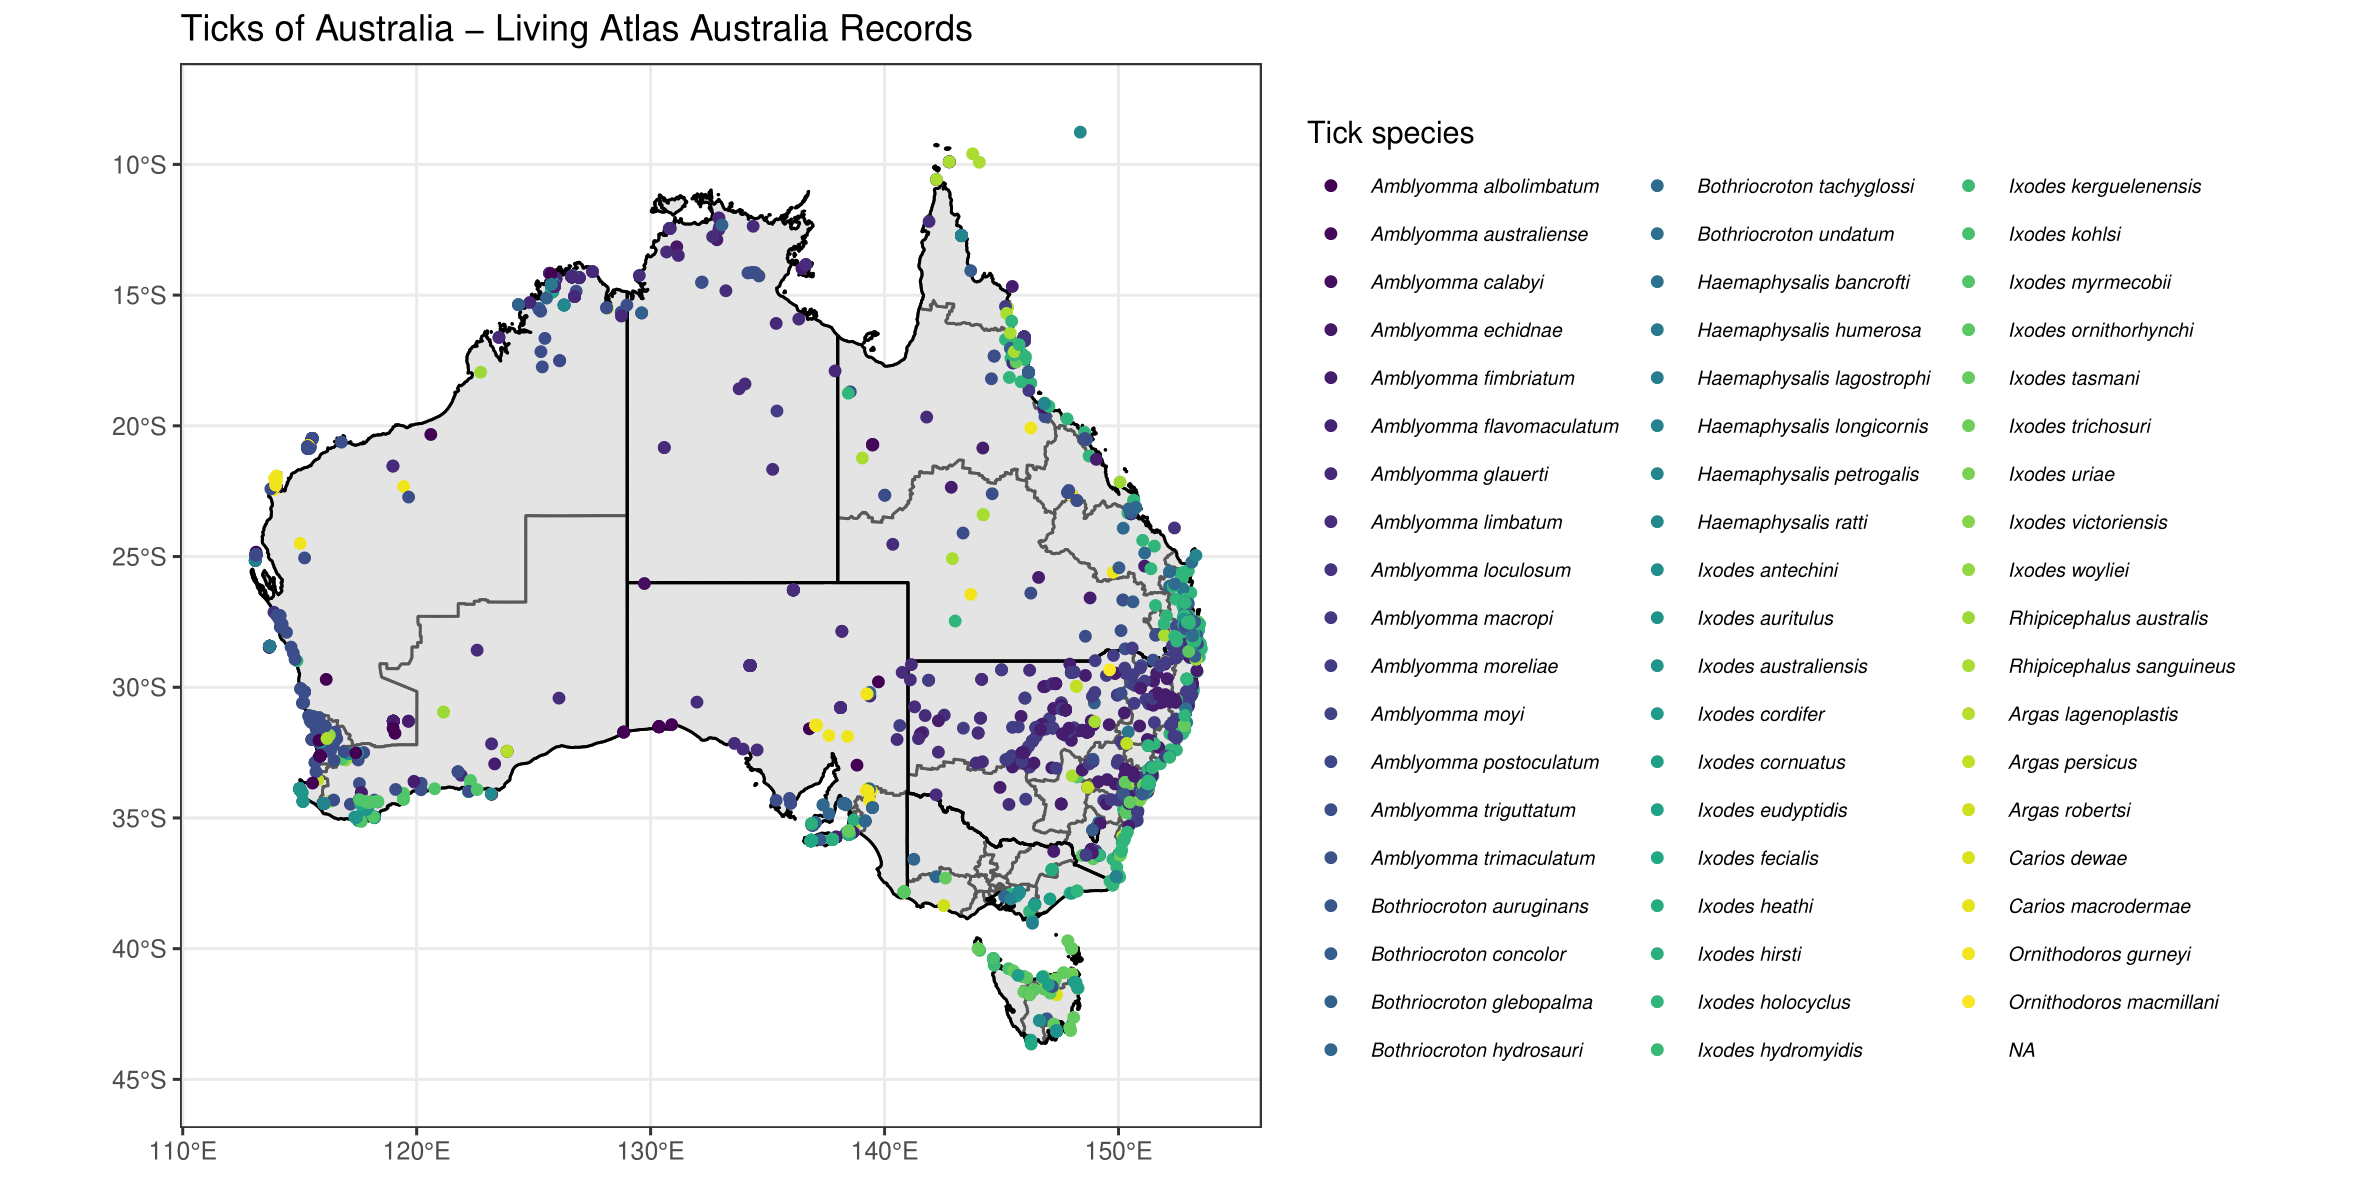
\includegraphics[width=0.95\linewidth]{figures/ms-figs-appendix/FigA-2.1} \caption[Records of Australian ticks from Atlas of Living Australia]{Occurrence map of ticks (Acari: Ixodida) records sourced from the Atlas of Living Australia (www.ala.org.au), data has not been curated.}\label{fig:FA21}
\end{figure}

\newpage

\begin{landscape}\begingroup\fontsize{7.5}{9.5}\selectfont

\begin{longtable}[t]{l>{}lllllll}
\caption[Genetic sequences generated from Australian ticks.]{\label{tab:T2MLSTseqs}Genetic sequences generated from Australian ticks using a multi-locus sequence typing approach. Nucleotide data has been deposited in GenBank with accession numbers of specimens included in the table. Host spcies: Short-beaked echidna (\textit{Tachyglossus aculeatus}); Platypus (\textit{Ornithorhynchus anatinus}); Common wombat (\textit{Vombatus ursinus}); Northern brown bandicoot (\textit{Isoodon macrourus}); Eastern barred bandicoot (\textit{Perameles gunnii}); Long-nosed bandicoot (\textit{Perameles nasuta}); Tasmanian Devil (\textit{Sarcophilus harrisii});  Dog (\textit{Canis lupus familiaris}); Cat (\textit{Felis catus}); Eastern ringtail possum (\textit{Pseudocheirus peregrinus}); Koala (\textit{Phascolarctos  cinereus}); Eastern grey kangaroo (\textit{Macropus giganteus}); Lace Monitor (\textit{Varanus varius}); Bobtail (\textit{Tiliqua rugosa}).}\\
\toprule
Target gene & Organism & Isolate & Host & Country & Note & Development stage & Genbank\\
\midrule
\endfirsthead
\caption[]{\label{tab:T2MLSTseqs}Genetic sequences generated from Australian ticks using a multi-locus sequence typing approach. Nucleotide data has been deposited in GenBank with accession numbers of specimens included in the table. Host spcies: Short-beaked echidna (\textit{Tachyglossus aculeatus}); Platypus (\textit{Ornithorhynchus anatinus}); Common wombat (\textit{Vombatus ursinus}); Northern brown bandicoot (\textit{Isoodon macrourus}); Eastern barred bandicoot (\textit{Perameles gunnii}); Long-nosed bandicoot (\textit{Perameles nasuta}); Tasmanian Devil (\textit{Sarcophilus harrisii});  Dog (\textit{Canis lupus familiaris}); Cat (\textit{Felis catus}); Eastern ringtail possum (\textit{Pseudocheirus peregrinus}); Koala (\textit{Phascolarctos  cinereus}); Eastern grey kangaroo (\textit{Macropus giganteus}); Lace Monitor (\textit{Varanus varius}); Bobtail (\textit{Tiliqua rugosa}). \textit{(continued)}}\\
\toprule
Target gene & Organism & Isolate & Host & Country & Note & Development stage & Genbank\\
\midrule
\endhead

\endfoot
\bottomrule
\endlastfoot
COX1 & \em{Bothriocroton tachyglossi} & ACF1 & Short-beaked echidna & Australia: Queensland & PI1268 & Female & OM840098\\
COX1 & \em{Bothriocroton tachyglossi} & ACF3 & Short-beaked echidna & Australia: Queensland & PI1268 & Female & OM840099\\
COX1 & \em{Ixodes ornithorhynchi} & IOF3 & Platypus & Australia: Queensland & PI419 & Female & OM840100\\
COX1 & \em{Ixodes ornithorhynchi} & IOF4 & Platypus & Australia: Queensland & PI419 & Female & OM840101\\
COX1 & \em{Ixodes ornithorhynchi} & IOF5 & Platypus & Australia: Queensland & PI419 & Female & OM840102\\
COX1 & \em{Bothriocroton auruginans} & BAF5 & Common wombat & Australia: Victoria & PI1382 & Female & OM840103\\
COX1 & \em{Bothriocroton auruginans} & BAF6 & Common wombat & Australia: Victoria & PI1382 & Female & OM840104\\
COX1 & \em{Haemaphysalis humerosa} & HHM1 & Northern brown bandicoot & Australia: Northern Territory & PI797 & Male & OM840105\\
COX1 & \em{Ixodes tasmani} & ITF6 & Eastern barred bandicoot & Australia: Tasmania & PI321 & Female & OM840106\\
COX1 & \em{Ixodes tasmani} & ITF10 & Eastern barred bandicoot & Australia: Tasmania & PI321 & Female & OM840107\\
COX1 & \em{Ixodes tasmani} & ITN6 & Eastern barred bandicoot & Australia: Tasmania & PI321 & Nymph & OM840108\\
COX1 & \em{Ixodes holocyclus} & B1 & Long-nosed bandicoot & Australia: New South Wales & PI387 & Female & OM840109\\
COX1 & \em{Ixodes holocyclus} & B2 & Long-nosed bandicoot & Australia: New South Wales & PI1592 & Female & OM840110\\
COX1 & \em{Ixodes tasmani} & B8 & Long-nosed bandicoot & Australia: New South Wales & PI1132 & Nymph & OM840111\\
COX1 & \em{Ixodes tasmani} & B16 & Bandicoot sp. & Australia: Tasmania & PI319 & Female & OM840112\\
COX1 & \em{Ixodes holocyclus} & B57 & Long-nosed bandicoot & Australia: New South Wales & PI1129 & Nymph & OM840113\\
COX1 & \em{Ixodes tasmani} & B62 & Long-nosed bandicoot & Australia: Queensland & PI1260 & Nymph & OM840114\\
COX1 & \em{Ixodes tasmani} & B63 & Long-nosed bandicoot & Australia: Queensland & PI1260 & Nymph & OM840115\\
COX1 & \em{Ixodes tasmani} & B64 & Long-nosed bandicoot & Australia: Queensland & PI1260 & Nymph & OM840116\\
COX1 & \em{Haemaphysalis bancrofti} & B77 & Long-nosed bandicoot & Australia: New South Wales & PI1388 & Female & OM840117\\
COX1 & \em{Ixodes tasmani} & B87 & Eastern barred bandicoot & Australia: Tasmania & PI321 & Female & OM840118\\
COX1 & \em{Ixodes tasmani} & B88 & Eastern barred bandicoot & Australia: Tasmania & PI321 & Female & OM840119\\
COX1 & \em{Ixodes tasmani} & B89 & Eastern barred bandicoot & Australia: Tasmania & PI321 & Female & OM840120\\
COX1 & \em{Haemaphysalis bancrofti} & B110 & Long-nosed bandicoot & Australia: New South Wales & PI771 & Nymph & OM840121\\
COX1 & \em{Ixodes tasmani} & TD1 & Tasmanian Devil & Australia: Tasmania & PI2105 & Nymph & OM840122\\
COX1 & \em{Ixodes tasmani} & TD2 & Tasmanian Devil & Australia: Tasmania & PI2105 & Nymph & OM840123\\
COX1 & \em{Ixodes tasmani} & TD3 & Tasmanian Devil & Australia: Tasmania & PI2105 & Nymph & OM840124\\
COX1 & \em{Ixodes tasmani} & TD5 & Tasmanian Devil & Australia: Tasmania & PI2105 & Female & OM840125\\
COX1 & \em{Ixodes tasmani} & TD6 & Tasmanian Devil & Australia: Tasmania & PI2106 & Nymph & OM840126\\
COX1 & \em{Ixodes tasmani} & TD7 & Tasmanian Devil & Australia: Tasmania & PI2107 & Female & OM840127\\
COX1 & \em{Ixodes tasmani} & TD8 & Tasmanian Devil & Australia: Tasmania & PI2108 & Female & OM840128\\
COX1 & \em{Ixodes tasmani} & TD9 & Tasmanian Devil & Australia: Tasmania & PI2109 & Female & OM840129\\
COX1 & \em{Ixodes tasmani} & TD10 & Tasmanian Devil & Australia: Tasmania & PI2110 & Female & OM840130\\
COX1 & \em{Ixodes fecialis} & TD12 & Tasmanian Devil & Australia: Tasmania & PI2112 & Female & OM840131\\
COX1 & \em{Ixodes fecialis} & TD13 & Tasmanian Devil & Australia: Tasmania & PI2113 & Nymph & OM840132\\
COX1 & \em{Ixodes fecialis} & TD14 & Tasmanian Devil & Australia: Tasmania & PI2114 & Female & OM840133\\
COX1 & \em{Ixodes tasmani} & TD15 & Tasmanian Devil & Australia: Tasmania & PI2115 & Female & OM840134\\
COX1 & \em{Amblyomma triguttatum} & AT2F & Questing & Australia: Yanchep, Western Australia &  & Female & MN106717\\
COX1 & \em{Amblyomma triguttatum} & AT3M & Questing & Australia: Yanchep, Western Australia &  & Male & MN106719\\
COX1 & \em{Amblyomma triguttatum} & AT4M & Questing & Australia: Yanchep, Western Australia &  & Male & MN106718\\
COX1 & \em{Bothriocroton auruginans} & BA1F & Common wombat & Australia: Trafalgar, Victoria &  & Female & MN106720\\
COX1 & \em{Bothriocroton auruginans} & BA2F & Common wombat & Australia: Trafalgar, Victoria &  & Female & MN106721\\
COX1 & \em{Haemaphysalis bancrofti} & HB2F & Long-nosed bandicoot & Australia: Stony Chute, New South Wales &  & Female & MN106722\\
COX1 & \em{Haemaphysalis bancrofti} & HB3N & Long-nosed bandicoot & Australia: Stony Chute, New South Wales &  & Nymph & MN106723\\
COX1 & \em{Haemaphysalis humerosa} & HH1N & Northern brown bandicoot & Australia: Beerwah, Queensland &  & Nymph & MN106726\\
COX1 & \em{Haemaphysalis humerosa} & HH3M & Northern brown bandicoot & Australia: Palmerston, Northern Territory &  & Male & MN106724\\
COX1 & \em{Haemaphysalis humerosa} & HH4M & Northern brown bandicoot & Australia: Palmerston, Northern Territory &  & Male & MN106725\\
COX1 & \em{Ixodes cornuatus} & IC1F & Dog & Australia: Port Sorrell, Tasmania &  & Female & MN106727\\
COX1 & \em{Ixodes hirsti} & IHi1F & Cat & Australia: Port Sorrell, Tasmania &  & Female & MN106728\\
COX1 & \em{Ixodes holocyclus} & Q92 & Questing & Australia: Springbrook, Queensland &  & Female & MN106729\\
COX1 & \em{Ixodes holocyclus} & Q93 & Questing & Australia: Springbrook, Queensland &  & Male & MN106730\\
COX1 & \em{Ixodes tasmani} & C4IT & Tasmanian Devil & Australia: Tasmania &  & Female & MN106731\\
COX1 & \em{Ixodes tasmani} & WL1 & Eastern ringtail possum & Australia: Queensland &  &  & OM791407\\
COX1 & \em{Ixodes tasmani} & WL2 & Koala & Australia: Queensland &  &  & OM791408\\
COX1 & \em{Haemaphysalis bancrofti} & WL11 & Eastern grey kangaroo & Australia: Queensland &  &  & OM791409\\
COX1 & \em{Bothriocroton undatum} & WL18 & Lace Monitor & Australia: Queensland &  &  & OM791410\\
COX1 & \em{Bothriocroton tachyglossi} & WL19 & Lace Monitor & Australia: Queensland &  &  & OM791411\\
COX1 & \em{Bothriocroton undatum} & WL20 & Lace Monitor & Australia: Queensland &  &  & OM791412\\
COX1 & \em{Bothriocroton tachyglossi} & WL30 & Short-beaked echidna & Australia: Queensland &  &  & OM791413\\
COX1 & \em{Bothriocroton tachyglossi} & WL31 & Short-beaked echidna & Australia: Queensland &  &  & OM791414\\
COX1 & \em{Bothriocroton tachyglossi} & WL32 & Short-beaked echidna & Australia: Queensland &  &  & OM791415\\
COX1 & \em{Bothriocroton tachyglossi} & WL33 & Short-beaked echidna & Australia: Queensland &  &  & OM791416\\
COX1 & \em{Bothriocroton tachyglossi} & WL34 & Short-beaked echidna & Australia: Queensland &  &  & OM791417\\
COX1 & \em{Bothriocroton tachyglossi} & WL35 & Short-beaked echidna & Australia: Queensland &  &  & OM791418\\
COX1 & \em{Bothriocroton tachyglossi} & WL36 & Short-beaked echidna & Australia: Queensland &  &  & OM791419\\
COX1 & \em{Bothriocroton tachyglossi} & WL37 & Short-beaked echidna & Australia: Queensland &  &  & OM791420\\
COX1 & \em{Bothriocroton tachyglossi} & WL38 & Short-beaked echidna & Australia: Queensland &  &  & OM791421\\
COX1 & \em{Bothriocroton tachyglossi} & WL39 & Short-beaked echidna & Australia: Queensland &  &  & OM791422\\
COX1 & \em{Bothriocroton tachyglossi} & WL40 & Short-beaked echidna & Australia: Queensland &  &  & OM791423\\
COX1 & \em{Bothriocroton tachyglossi} & WL41 & Short-beaked echidna & Australia: Queensland &  &  & OM791424\\
COX1 & \em{Bothriocroton tachyglossi} & WL42 & Short-beaked echidna & Australia: Queensland &  &  & OM791425\\
COX1 & \em{Bothriocroton tachyglossi} & WL44 & Short-beaked echidna & Australia: Queensland &  &  & OM791426\\
COX1 & \em{Bothriocroton tachyglossi} & WL45 & Short-beaked echidna & Australia: Queensland &  &  & OM791427\\
COX1 & \em{Bothriocroton tachyglossi} & WL46 & Short-beaked echidna & Australia: Queensland &  &  & OM791428\\
COX1 & \em{Amblyomma fimbriatum} & WL51 & Lace Monitor & Australia: Queensland &  &  & OM791429\\
COX1 & \em{Amblyomma fimbriatum} & WL52 & Lace Monitor & Australia: Queensland &  &  & OM791430\\
COX1 & \em{Bothriocroton undatum} & WL53 & Lace Monitor & Australia: Queensland &  &  & OM791431\\
COX1 & \em{Bothriocroton undatum} & WL54 & Lace Monitor & Australia: Queensland &  &  & OM791432\\
COX1 & \em{Bothriocroton undatum} & WL55 & Lace Monitor & Australia: Queensland &  &  & OM791433\\
COX1 & \em{Amblyomma fimbriatum} & WL56 & Lace Monitor & Australia: Queensland &  &  & OM791434\\
COX1 & \em{Bothriocroton undatum} & WL57 & Lace Monitor & Australia: Queensland &  &  & OM791435\\
COX1 & \em{Bothriocroton undatum} & WL58 & Lace Monitor & Australia: Queensland &  &  & OM791436\\
COX1 & \em{Bothriocroton undatum} & WL60 & Lace Monitor & Australia: Queensland &  &  & OM791437\\
16S rRNA & \em{Amblyomma triguttatum} & AT1F & Questing & Australia: Yanchep, Western Australia &  &  & OM830384\\
16S rRNA & \em{Amblyomma triguttatum} & AT2F & Questing & Australia: Yanchep, Western Australia &  &  & OM830385\\
16S rRNA & \em{Amblyomma triguttatum} & AT3M & Questing & Australia: Yanchep, Western Australia &  &  & OM830386\\
16S rRNA & \em{Amblyomma triguttatum} & AT4M & Questing & Australia: Yanchep, Western Australia &  &  & OM830387\\
16S rRNA & \em{Amblyomma triguttatum} & AT5N & Questing & Australia: Yanchep, Western Australia &  &  & OM830388\\
16S rRNA & \em{Bothriocroton auruginans} & BA1F & Common wombat & Australia: Trafalgar, Victoria &  &  & OM830389\\
16S rRNA & \em{Bothriocroton auruginans} & BA2F & Common wombat & Australia: Trafalgar, Victoria &  &  & OM830390\\
16S rRNA & \em{Haemaphysalis bancrofti} & HB2F & Long-nosed bandicoot & Australia: Stony Chute, New South Wales &  &  & OM830391\\
16S rRNA & \em{Haemaphysalis bancrofti} & HB3F & Long-nosed bandicoot & Australia: Stony Chute, New South Wales &  &  & OM830392\\
16S rRNA & \em{Haemaphysalis humerosa} & HH1M & Northern brown bandicoot & Australia: Beerwah, Queensland &  &  & OM830393\\
16S rRNA & \em{Haemaphysalis humerosa} & HH3M & Northern brown bandicoot & Australia: Palmerston, Northern Territory &  &  & OM830394\\
16S rRNA & \em{Haemaphysalis humerosa} & HH4M & Northern brown bandicoot & Australia: Palmerston, Northern Territory &  &  & OM830395\\
16S rRNA & \em{Ixodes cornuatus} & IC1F & Dog & Australia: Port Sorrell, Tasmania &  &  & OM830396\\
16S rRNA & \em{Ixodes hirsti} & IHi1F & Cat & Australia: Port Sorrell, Tasmania &  &  & OM830397\\
16S rRNA & \em{Ixodes holocyclus} & IH1F & Long-nosed bandicoot & Australia: New South Wales &  &  & OM830398\\
16S rRNA & \em{Ixodes holocyclus} & Q92 & Questing & Australia: Springbrook, Queensland &  &  & OM830399\\
16S rRNA & \em{Ixodes holocyclus} & Q93 & Questing & Australia: Springbrook, Queensland &  &  & OM830400\\
16S rRNA & \em{Ixodes tasmani} & IT3 & Tasmanian Devil & Australia: Tasmania &  &  & OM830401\\
16S rRNA & \em{Ixodes tasmani} & WL1 & Eastern ringtail possum & Australia: Queensland &  &  & OM830402\\
16S rRNA & \em{Ixodes tasmani} & WL2 & Koala & Australia: Queensland &  &  & OM830403\\
16S rRNA & \em{Haemaphysalis bancrofti} & WL11 & Eastern grey kangaroo & Australia: Queensland &  &  & OM830404\\
16S rRNA & \em{Bothriocroton tachyglossi} & WL19 & Lace Monitor & Australia: Queensland &  &  & OM830405\\
16S rRNA & \em{Bothriocroton undatum} & WL20 & Lace Monitor & Australia: Queensland &  &  & OM830406\\
16S rRNA & \em{Bothriocroton tachyglossi} & WL30 & Short-beaked echidna & Australia: Queensland &  &  & OM830407\\
16S rRNA & \em{Bothriocroton tachyglossi} & WL31 & Short-beaked echidna & Australia: Queensland &  &  & OM830408\\
16S rRNA & \em{Bothriocroton tachyglossi} & WL32 & Short-beaked echidna & Australia: Queensland &  &  & OM830409\\
16S rRNA & \em{Bothriocroton tachyglossi} & WL33 & Short-beaked echidna & Australia: Queensland &  &  & OM830410\\
16S rRNA & \em{Bothriocroton tachyglossi} & WL34 & Short-beaked echidna & Australia: Queensland &  &  & OM830411\\
16S rRNA & \em{Bothriocroton tachyglossi} & WL35 & Short-beaked echidna & Australia: Queensland &  &  & OM830412\\
16S rRNA & \em{Bothriocroton tachyglossi} & WL36 & Short-beaked echidna & Australia: Queensland &  &  & OM830413\\
16S rRNA & \em{Bothriocroton tachyglossi} & WL37 & Short-beaked echidna & Australia: Queensland &  &  & OM830414\\
16S rRNA & \em{Bothriocroton tachyglossi} & WL38 & Short-beaked echidna & Australia: Queensland &  &  & OM830415\\
16S rRNA & \em{Bothriocroton tachyglossi} & WL39 & Short-beaked echidna & Australia: Queensland &  &  & OM830416\\
16S rRNA & \em{Bothriocroton tachyglossi} & WL41 & Short-beaked echidna & Australia: Queensland &  &  & OM830417\\
16S rRNA & \em{Bothriocroton tachyglossi} & WL42 & Short-beaked echidna & Australia: Queensland &  &  & OM830418\\
16S rRNA & \em{Bothriocroton tachyglossi} & WL44 & Short-beaked echidna & Australia: Queensland &  &  & OM830419\\
16S rRNA & \em{Bothriocroton tachyglossi} & WL45 & Short-beaked echidna & Australia: Queensland &  &  & OM830420\\
16S rRNA & \em{Bothriocroton tachyglossi} & WL46 & Short-beaked echidna & Australia: Queensland &  &  & OM830421\\
16S rRNA & \em{Amblyomma fimbriatum} & WL51 & Lace Monitor & Australia: Queensland &  &  & OM830422\\
16S rRNA & \em{Amblyomma fimbriatum} & WL52 & Lace Monitor & Australia: Queensland &  &  & OM830423\\
16S rRNA & \em{Bothriocroton undatum} & WL53 & Lace Monitor & Australia: Queensland &  &  & OM830424\\
16S rRNA & \em{Bothriocroton undatum} & WL54 & Lace Monitor & Australia: Queensland &  &  & OM830425\\
16S rRNA & \em{Bothriocroton undatum} & WL55 & Lace Monitor & Australia: Queensland &  &  & OM830426\\
16S rRNA & \em{Amblyomma fimbriatum} & WL56 & Lace Monitor & Australia: Queensland &  &  & OM830427\\
16S rRNA & \em{Bothriocroton undatum} & WL57 & Lace Monitor & Australia: Queensland &  &  & OM830428\\
16S rRNA & \em{Bothriocroton undatum} & WL58 & Lace Monitor & Australia: Queensland &  &  & OM830429\\
12S rRNA & \em{Amblyomma triguttatum} & AT1F & Questing & Australia: Yanchep, Western Australia &  &  & OM830716\\
12S rRNA & \em{Amblyomma triguttatum} & AT2F & Questing & Australia: Yanchep, Western Australia &  &  & OM830717\\
12S rRNA & \em{Amblyomma triguttatum} & AT3M & Questing & Australia: Yanchep, Western Australia &  &  & OM830718\\
12S rRNA & \em{Amblyomma triguttatum} & AT4M & Questing & Australia: Yanchep, Western Australia &  &  & OM830719\\
12S rRNA & \em{Amblyomma triguttatum} & AT5N & Questing & Australia: Yanchep, Western Australia &  &  & OM830720\\
12S rRNA & \em{Bothriocroton auruginans} & BA1F & Common wombat & Australia: Trafalgar, Victoria &  &  & OM830721\\
12S rRNA & \em{Bothriocroton auruginans} & BA2F & Common wombat & Australia: Trafalgar, Victoria &  &  & OM830722\\
12S rRNA & \em{Haemaphysalis bancrofti} & HB2F & Long-nosed bandicoot & Australia: Stony Chute, New South Wales &  &  & OM830723\\
12S rRNA & \em{Haemaphysalis bancrofti} & HB3F & Long-nosed bandicoot & Australia: Stony Chute, New South Wales &  &  & OM830724\\
12S rRNA & \em{Haemaphysalis humerosa} & HH1M & Northern brown bandicoot & Australia: Beerwah, Queensland &  &  & OM830725\\
12S rRNA & \em{Haemaphysalis humerosa} & HH3M & Northern brown bandicoot & Australia: Palmerston, Northern Territory &  &  & OM830726\\
12S rRNA & \em{Haemaphysalis humerosa} & HH4M & Northern brown bandicoot & Australia: Palmerston, Northern Territory &  &  & OM830727\\
12S rRNA & \em{Ixodes cornuatus} & IC1F & Dog & Australia: Port Sorrell, Tasmania &  &  & OM830728\\
12S rRNA & \em{Ixodes hirsti} & IHi1F & Cat & Australia: Port Sorrell, Tasmania &  &  & OM830729\\
12S rRNA & \em{Ixodes holocyclus} & IH1F & Long-nosed bandicoot & Australia: New South Wales &  &  & OM830730\\
12S rRNA & \em{Ixodes holocyclus} & Q92 & Questing & Australia: Springbrook, Queensland &  &  & OM830731\\
12S rRNA & \em{Ixodes holocyclus} & Q93 & Questing & Australia: Springbrook, Queensland &  &  & OM830732\\
12S rRNA & \em{Ixodes tasmani} & IT3 & Tasmanian Devil & Australia: Tasmania &  &  & OM830733\\
12S rRNA & \em{Ixodes tasmani} & WL1 & Eastern ringtail possum & Australia: Queensland &  &  & OM830734\\
12S rRNA & \em{Ixodes tasmani} & WL2 & Koala & Australia: Queensland &  &  & OM830735\\
12S rRNA & \em{Haemaphysalis bancrofti} & WL11 & Eastern grey kangaroo & Australia: Queensland &  &  & OM830736\\
12S rRNA & \em{Bothriocroton undatum} & WL18 & Lace Monitor & Australia: Queensland &  &  & OM830737\\
12S rRNA & \em{Bothriocroton tachyglossi} & WL19 & Lace Monitor & Australia: Queensland &  &  & OM830738\\
12S rRNA & \em{Bothriocroton undatum} & WL20 & Lace Monitor & Australia: Queensland &  &  & OM830739\\
12S rRNA & \em{Bothriocroton tachyglossi} & WL30 & Short-beaked echidna & Australia: Queensland &  &  & OM830740\\
12S rRNA & \em{Bothriocroton tachyglossi} & WL31 & Short-beaked echidna & Australia: Queensland &  &  & OM830741\\
12S rRNA & \em{Bothriocroton tachyglossi} & WL32 & Short-beaked echidna & Australia: Queensland &  &  & OM830742\\
12S rRNA & \em{Bothriocroton tachyglossi} & WL33 & Short-beaked echidna & Australia: Queensland &  &  & OM830743\\
12S rRNA & \em{Bothriocroton tachyglossi} & WL34 & Short-beaked echidna & Australia: Queensland &  &  & OM830744\\
12S rRNA & \em{Bothriocroton tachyglossi} & WL35 & Short-beaked echidna & Australia: Queensland &  &  & OM830745\\
12S rRNA & \em{Bothriocroton tachyglossi} & WL36 & Short-beaked echidna & Australia: Queensland &  &  & OM830746\\
12S rRNA & \em{Bothriocroton tachyglossi} & WL37 & Short-beaked echidna & Australia: Queensland &  &  & OM830747\\
12S rRNA & \em{Bothriocroton tachyglossi} & WL38 & Short-beaked echidna & Australia: Queensland &  &  & OM830748\\
12S rRNA & \em{Bothriocroton tachyglossi} & WL39 & Short-beaked echidna & Australia: Queensland &  &  & OM830749\\
12S rRNA & \em{Bothriocroton tachyglossi} & WL40 & Short-beaked echidna & Australia: Queensland &  &  & OM830750\\
12S rRNA & \em{Bothriocroton tachyglossi} & WL41 & Short-beaked echidna & Australia: Queensland &  &  & OM830751\\
12S rRNA & \em{Bothriocroton tachyglossi} & WL42 & Short-beaked echidna & Australia: Queensland &  &  & OM830752\\
12S rRNA & \em{Bothriocroton tachyglossi} & WL44 & Short-beaked echidna & Australia: Queensland &  &  & OM830753\\
12S rRNA & \em{Bothriocroton tachyglossi} & WL45 & Short-beaked echidna & Australia: Queensland &  &  & OM830754\\
12S rRNA & \em{Bothriocroton tachyglossi} & WL46 & Short-beaked echidna & Australia: Queensland &  &  & OM830755\\
12S rRNA & \em{Amblyomma fimbriatum} & WL51 & Lace Monitor & Australia: Queensland &  &  & OM830756\\
12S rRNA & \em{Amblyomma fimbriatum} & WL52 & Lace Monitor & Australia: Queensland &  &  & OM830757\\
12S rRNA & \em{Bothriocroton undatum} & WL53 & Lace Monitor & Australia: Queensland &  &  & OM830758\\
12S rRNA & \em{Bothriocroton undatum} & WL54 & Lace Monitor & Australia: Queensland &  &  & OM830759\\
12S rRNA & \em{Bothriocroton undatum} & WL55 & Lace Monitor & Australia: Queensland &  &  & OM830760\\
12S rRNA & \em{Amblyomma fimbriatum} & WL56 & Lace Monitor & Australia: Queensland &  &  & OM830761\\
12S rRNA & \em{Bothriocroton undatum} & WL57 & Lace Monitor & Australia: Queensland &  &  & OM830762\\
12S rRNA & \em{Bothriocroton undatum} & WL58 & Lace Monitor & Australia: Queensland &  &  & OM830763\\
12S rRNA & \em{Bothriocroton undatum} & WL60 & Lace Monitor & Australia: Queensland &  &  & OM830764\\
18S rRNA & \em{Amblyomma albolimbatum} & R1 & Bobtail & Australia: Western Australia & PI982 & Female & OM756762\\
18S rRNA & \em{Amblyomma albolimbatum} & R2 & Bobtail & Australia: Western Australia & PI982 & Male & OM756763\\
18S rRNA & \em{Amblyomma albolimbatum} & R21 & Bobtail & Australia: Western Australia & PI1733 & Male & OM756764\\
18S rRNA & \em{Amblyomma albolimbatum} & R22 & Bobtail & Australia: Western Australia & PI1732 & Male & OM756765\\
18S rRNA & \em{Amblyomma fimbriatum} & WL52 & Lace Monitor & Australia: Queensland & PI1732 &  & OM756761\\
18S rRNA & \em{Amblyomma triguttatum} & ATT51 & Questing & Australia: Western Australia & ATT51 &  & OM756760\\*
\end{longtable}
\endgroup{}
\end{landscape}

\newpage

\begingroup\fontsize{7.5}{9.5}\selectfont

\begin{longtable}[t]{l>{}l|l>{}l}
\caption[GenBank accession numbers and species identification of sequences used to produce phylogenetic tree.]{\label{tab:T2genbank}GenBank accession numbers and species identification of sequences used to produce phylogenetic tree (Figure 2.5).}\\
\toprule
GenBank (reference) & Species (Reference) & GenBank (new) & Species (new)\\
\midrule
\endfirsthead
\caption[]{\label{tab:T2genbank}GenBank accession numbers and species identification of sequences used to produce phylogenetic tree (Figure 2.5). \textit{(continued)}}\\
\toprule
GenBank (reference) & Species (Reference) & GenBank (new) & Species (new)\\
\midrule
\endhead

\endfoot
\bottomrule
\endlastfoot
AB073725 & \em{Ixodes persulcatus} & MW665133 & \em{Ixodes holocyclus}\\
AB075955 & \em{Ixodes holocyclus} & MW665134 & \em{Ixodes tasmani}\\
AB087746 & \em{Ixodes uriae} & MW665135 & \em{Ixodes trichosuri}\\
AB113317 & \em{Amblyomma triguttatum} & MW665136 & \em{Ixodes trichosuri}\\
AF031851 & \em{Dermacentor variabilis} & MW665137 & \em{Ixodes tasmani}\\
AF031852 & \em{Haemaphysalis humerosa} & MW665138 & \em{Ixodes tasmani}\\
AF031853 & \em{Haemaphysalis longicornis} & MW665139 & \em{Ixodes australiensis}\\
AM410581 & \em{Ixodes uriae} & MW665140 & \em{Ixodes tasmani}\\
EF173724 & \em{Bothriocroton glebopalma} & MW665141 & \em{Ixodes antechini}\\
EF173725 & \em{Bothriocroton concolor} & MW665142 & \em{Ixodes tasmani}\\
EF173726 & \em{Bothriocroton undatum} & MW665143 & \em{Amblyomma triguttatum}\\
HG918113 & \em{Ixodes scapularis} & MW665144 & \em{Ixodes antechini}\\
IUU95907 & \em{Ixodes uriae} & MW665145 & \em{Amblyomma triguttatum}\\
JN863727 & \em{Bothriocroton concolor} & MW665146 & \em{Amblyomma triguttatum}\\
JN863728 & \em{Bothriocroton undatum} & MW665147 & \em{Amblyomma triguttatum}\\
JN863729 & \em{Robertsicus elaphensis} & MW665148 & \em{Amblyomma triguttatum}\\
JN863730 & \em{Amblyomma fimbriatum} & MW665149 & \em{Amblyomma triguttatum}\\
JN863731 & \em{Archaeocroton sphenodonti} & MW665150 & \em{Ixodes trichosuri}\\
JQ346679 & \em{Haemaphysalis doenitzi} & OM830716 & \em{Amblyomma triguttatum}\\
KC503255 & \em{Rhipicephalus australis} & OM830717 & \em{Amblyomma triguttatum}\\
KF197132 & \em{Ixodes ricinus} & OM830718 & \em{Amblyomma triguttatum}\\
KF583608 & \em{Haemaphysalis longicornis} & OM830719 & \em{Amblyomma triguttatum}\\
KJ000060 & \em{Ixodes pavlovskyi} & OM830720 & \em{Amblyomma triguttatum}\\
KM455964 & \em{Ixodes simplex} & OM830721 & \em{Bothriocroton auruginans}\\
MH043264 & \em{Ixodes holocyclus} & OM830722 & \em{Bothriocroton auruginans}\\
MH043265 & \em{Ixodes holocyclus} & OM830723 & \em{Haemaphysalis bancrofti}\\
MH043266 & \em{Ixodes holocyclus} & OM830724 & \em{Haemaphysalis bancrofti}\\
MH043267 & \em{Ixodes holocyclus} & OM830725 & \em{Haemaphysalis humerosa}\\
MH043268 & \em{Haemaphysalis bancrofti} & OM830726 & \em{Haemaphysalis humerosa}\\
MH043269 & \em{Ixodes tasmani} & OM830727 & \em{Haemaphysalis humerosa}\\
MH043270 & \em{Ixodes tasmani} & OM830728 & \em{Ixodes cornuatus}\\
MH043271 & \em{Ixodes tasmani} & OM830729 & \em{Ixodes hirsti}\\
NC\_002010 & \em{Ixodes hexagonus} & OM830730 & \em{Ixodes holocyclus}\\
U95858 & \em{Bothriocroton glebopalma} & OM830732 & \em{Ixodes holocyclus}\\
U95860 & \em{Bothriocroton hydrosauri} & OM830733 & \em{Ixodes tasmani}\\
 & \em{} & OM830734 & \em{Ixodes tasmani}\\
 & \em{} & OM830735 & \em{Ixodes tasmani}\\
 & \em{} & OM830736 & \em{Haemaphysalis bancrofti}\\
 & \em{} & OM830746 & \em{Bothriocroton tachyglossi}\\
 & \em{} & OM830756 & \em{Amblyomma fimbriatum}\\
 & \em{} & OM830757 & \em{Amblyomma fimbriatum}\\
 & \em{} & OM830761 & \em{Amblyomma fimbriatum}\\
 & \em{} & OM830762 & \em{Bothriocroton undatum}\\*
\end{longtable}
\endgroup{}

\newpage

\hypertarget{ch3supp}{%
\section{Chapter 3}\label{ch3supp}}

Supplementary material for Chapter \ref{wildlife-bacteria} on the Microbiome of Ticks and Wildlife.

\begin{table}[!h]

\caption[Summary of sequences obtained from bacterial amplicon sequencing.]{\label{tab:TA31}Summary of sequences obtained from bacterial next-generation sequencin.g}
\centering
\fontsize{8.5}{10.5}\selectfont
\begin{tabular}[t]{llllll}
\toprule
Bioinformatics step & Control (totals) & Sample (totals) & Blood & Tick & Tissue\\
\midrule
Sum input & 5534288 & 96969355 & 35160160 & 24844688 & 36964507\\
Mean input & 85143 & 152228 & 185053 & 95556 & 197671\\
Sum filtered & 3922421 & 70048790 & 24929182 & 19809370 & 25310238\\
Mean filtered & 60345 & 109967 & 131206 & 76190 & 135349\\
Filtered \% & 70.90\% & 72.20\% & 70.90\% & 79.70\% & 68.50\%\\
Sum denoised & 3906305 & 69477650 & 24758558 & 19753200 & 24965892\\
Mean denoised & 60097 & 109070 & 130308 & 75974 & 133507\\
Sum merged & 3815914 & 67183779 & 24028959 & 19127172 & 24027648\\
Mean merged & 58706 & 105469 & 126468 & 73566 & 128490\\
Merged \% & 69.00\% & 69.30\% & 68.30\% & 77.00\% & 65.00\%\\
Sum non-chimeric & 3719634 & 64186307 & 23061496 & 18368918 & 22755893\\
Mean non-chimeric & 57225 & 100763 & 121376 & 70650 & 121689\\
Input non-chimeric \% & 67.20\% & 66.20\% & 65.60\% & 73.90\% & 61.60\%\\
\bottomrule
\end{tabular}
\end{table}

\newpage

\begin{figure}
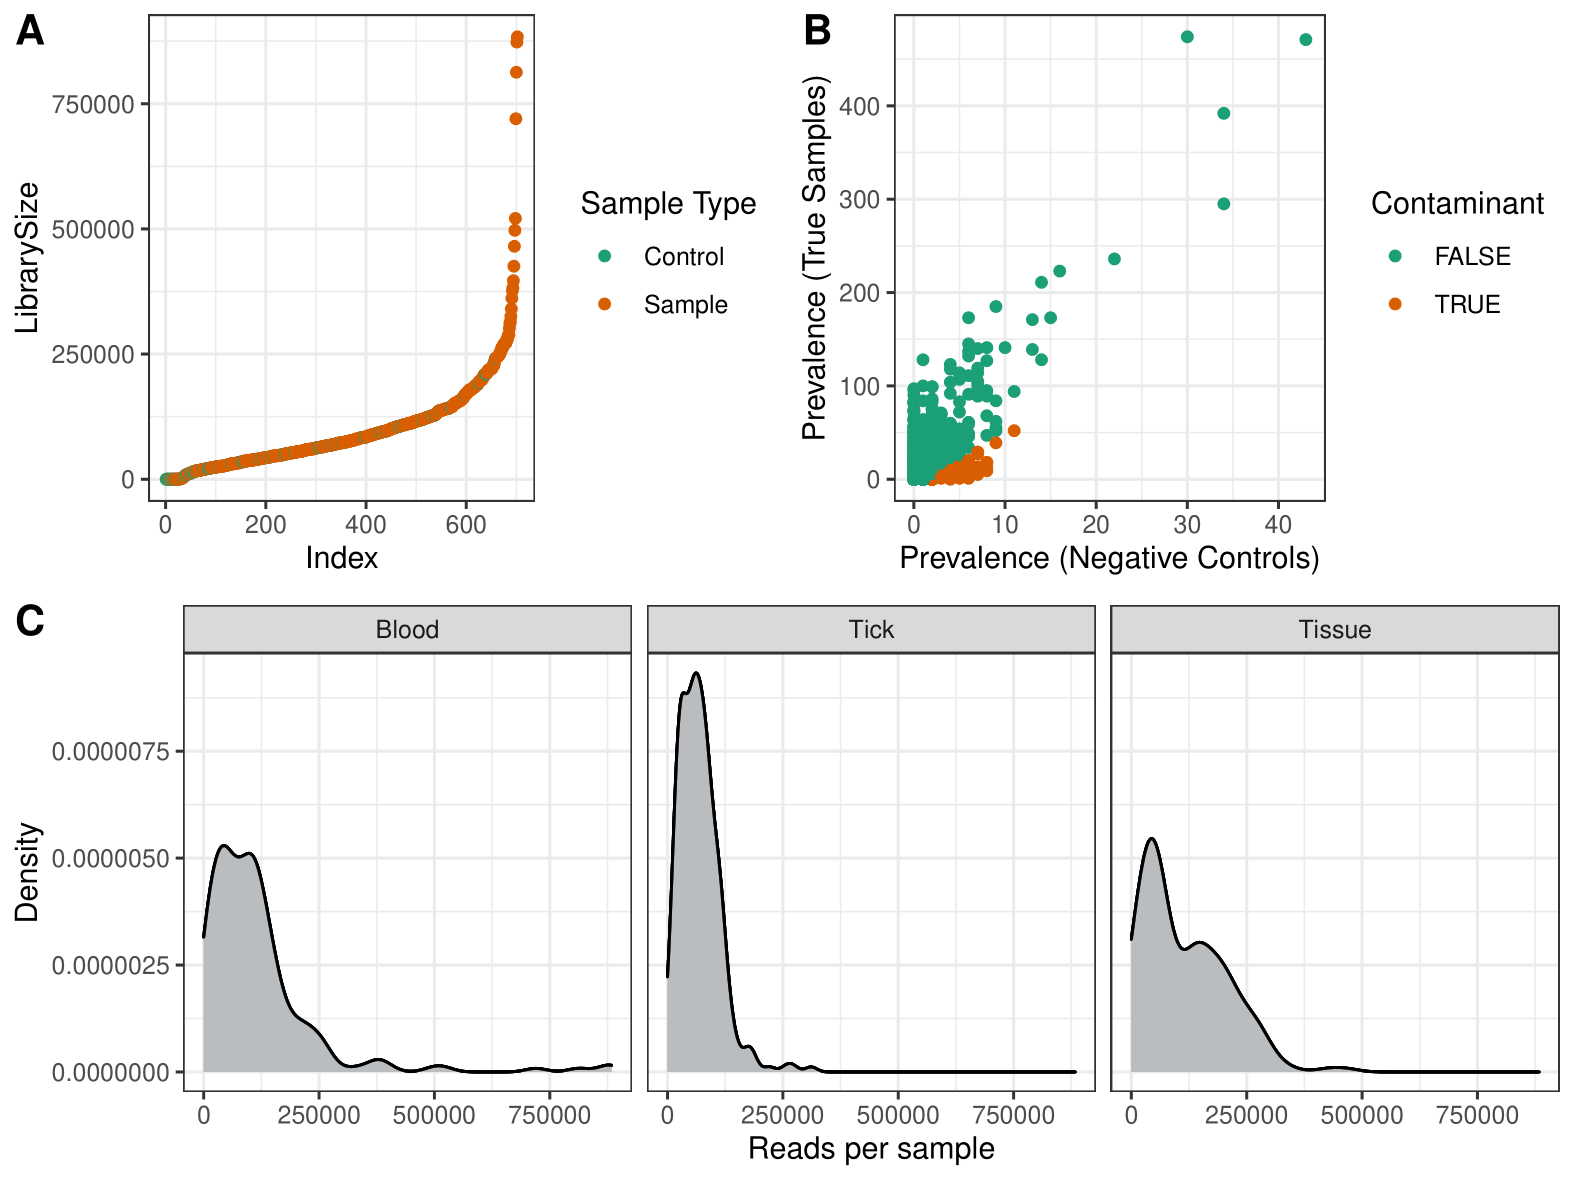
\includegraphics[width=0.95\linewidth]{figures/ms-figs-appendix/FigA-3.1} \caption[Summary of sequences obtained from bacterial metabarcoding of the 16S rRNA gene.]{Summary of sequences obtained form bacterial metabarcoding of the 16S rRNA gene (Illumina MiSeq). (A) Library size (i.e. number of sequences) obtained from samples. (B) Prevalence of contaminant ASVs as identified by `decontam` analysis in controls and samples. (C) Distribution of the number of reads in sample categories blood, tick and tissue.}\label{fig:FA31}
\end{figure}

\newpage

\begin{figure}
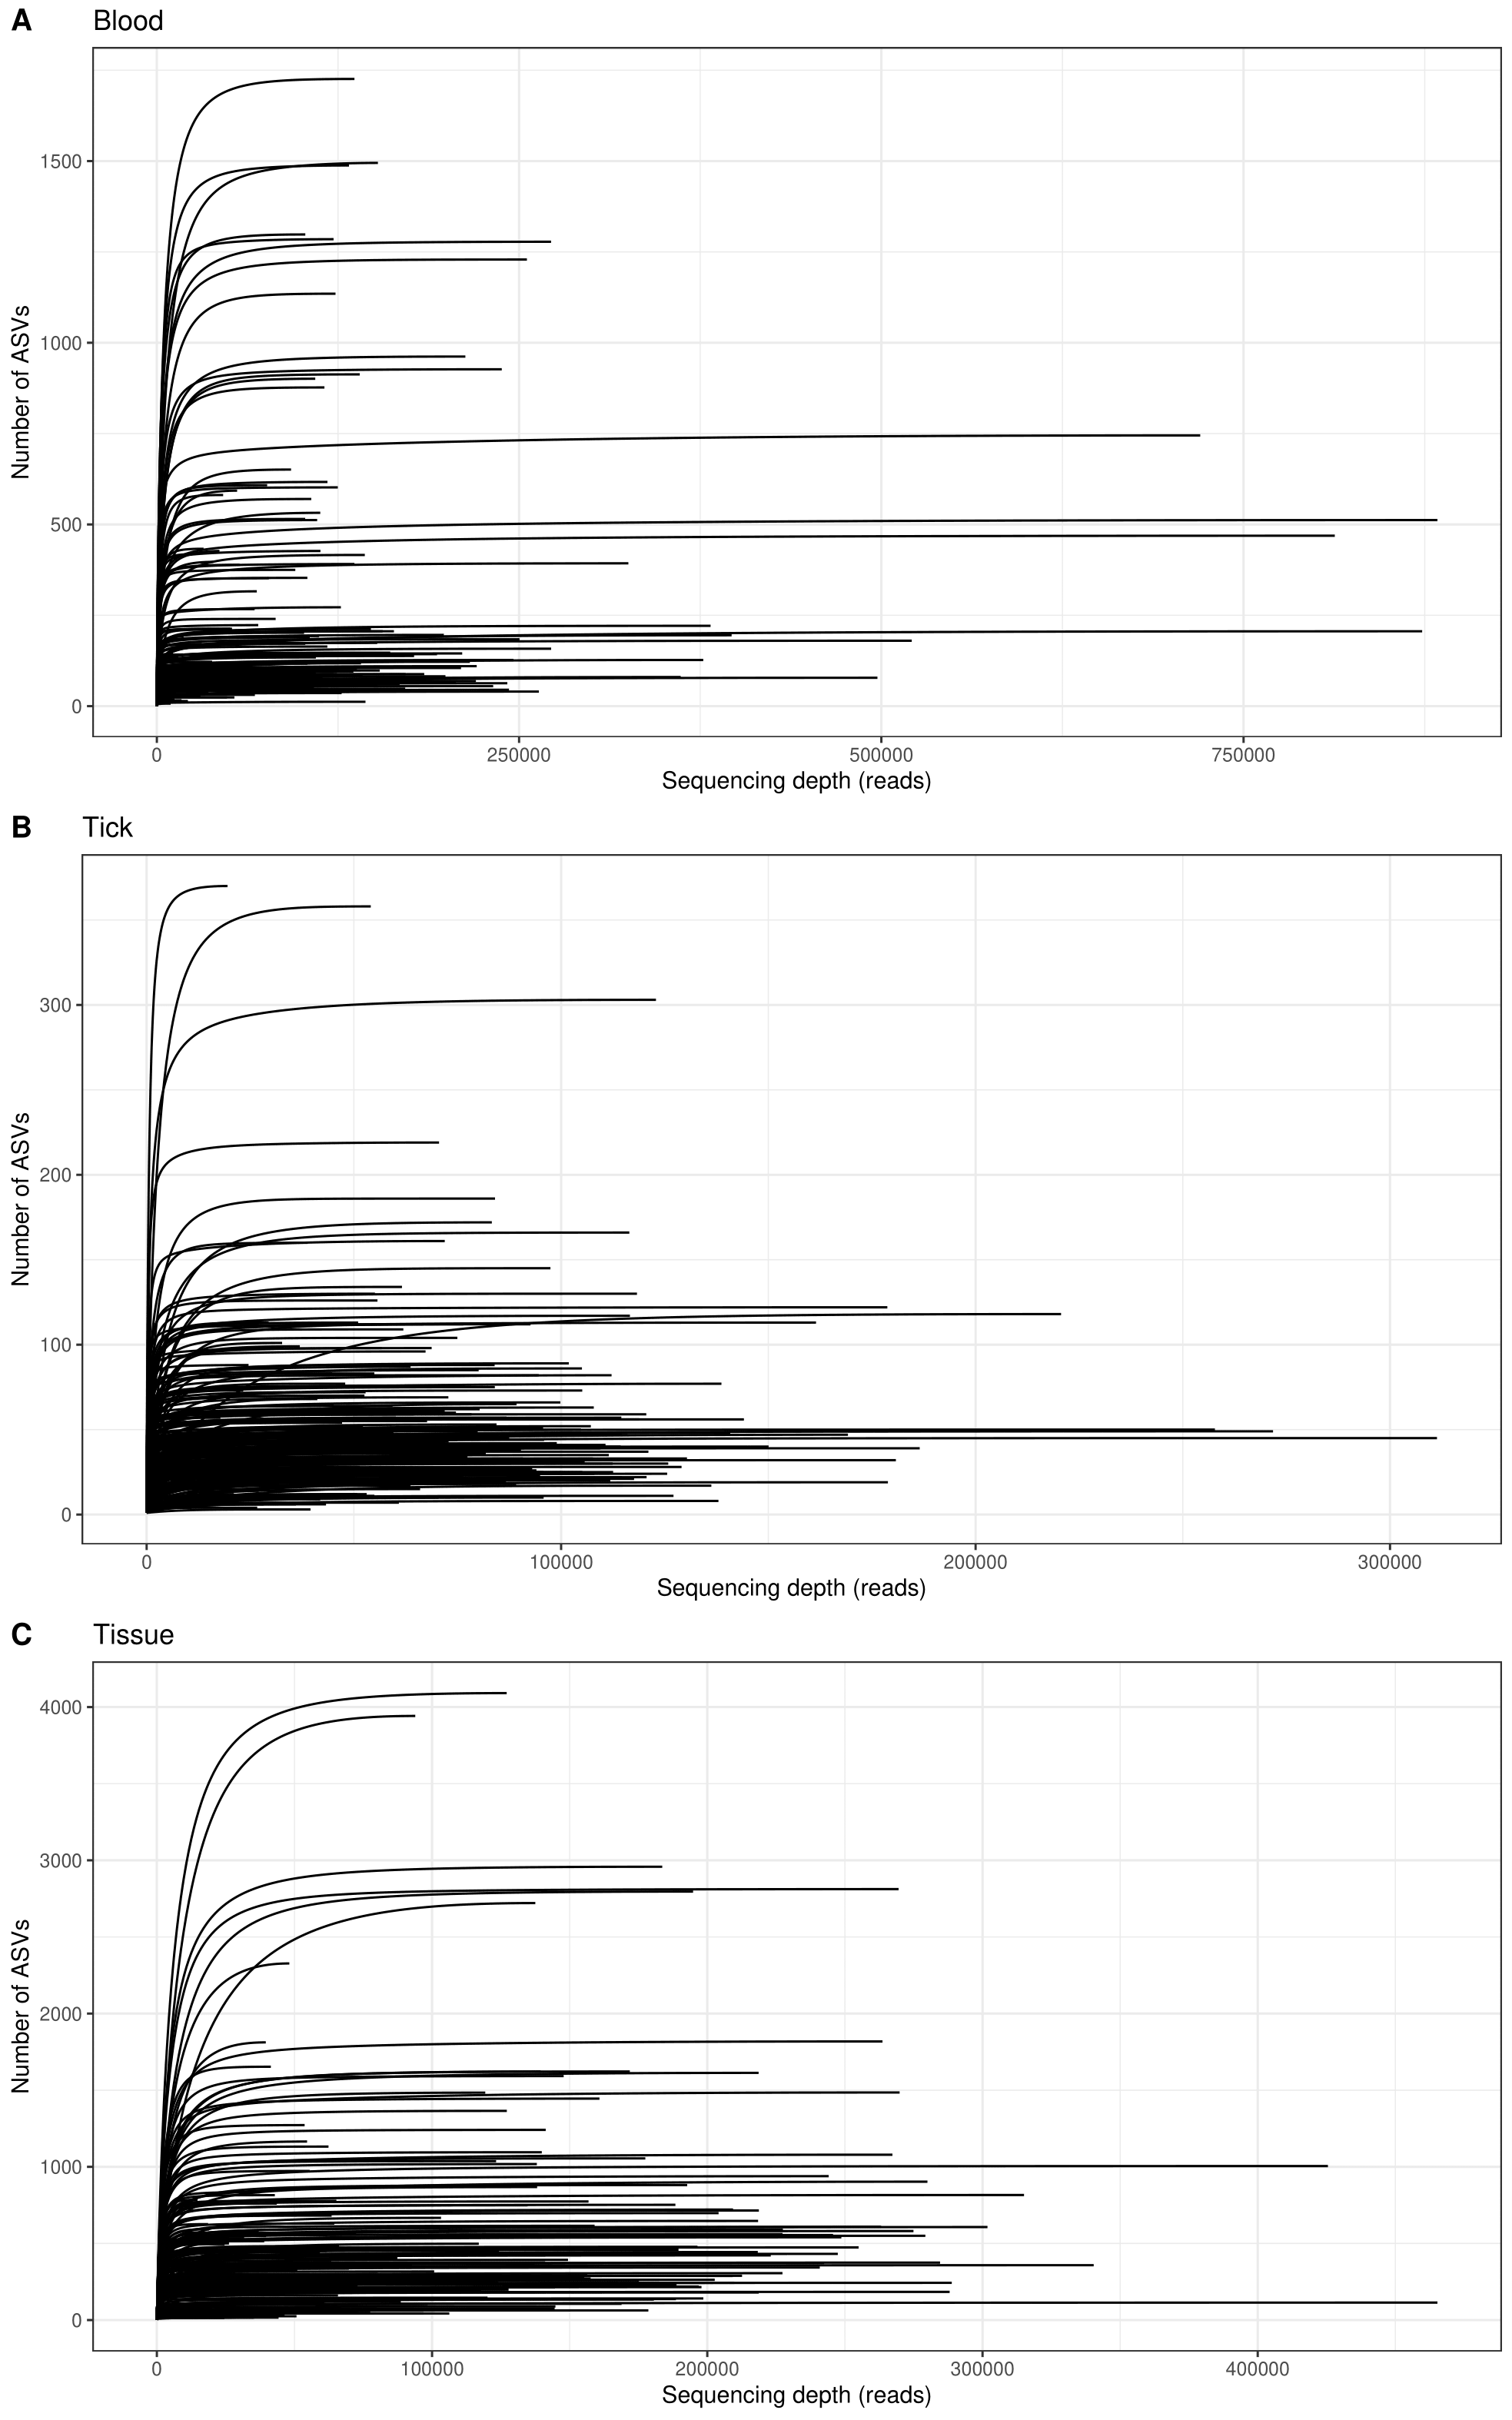
\includegraphics[width=0.85\linewidth]{figures/ms-figs-appendix/FigA-3.2} \caption[Rarefaction curves of bacterial 16S rRNA sequencing from wildlife samples.]{Rarefaction curves (number of ASVs) of wildlife blood, tick and tissue samples from bacterial 16S rRNA profiling (step size = 100). Rarefaction curves were used to determine how adequate sequencing depth was in detecting the complete theoretical suite of bacterial organisms present; of note, rarefaction plots excluded OTUs considered environmental contaminants (described methods).}\label{fig:FA32}
\end{figure}

\newpage

\begin{figure}
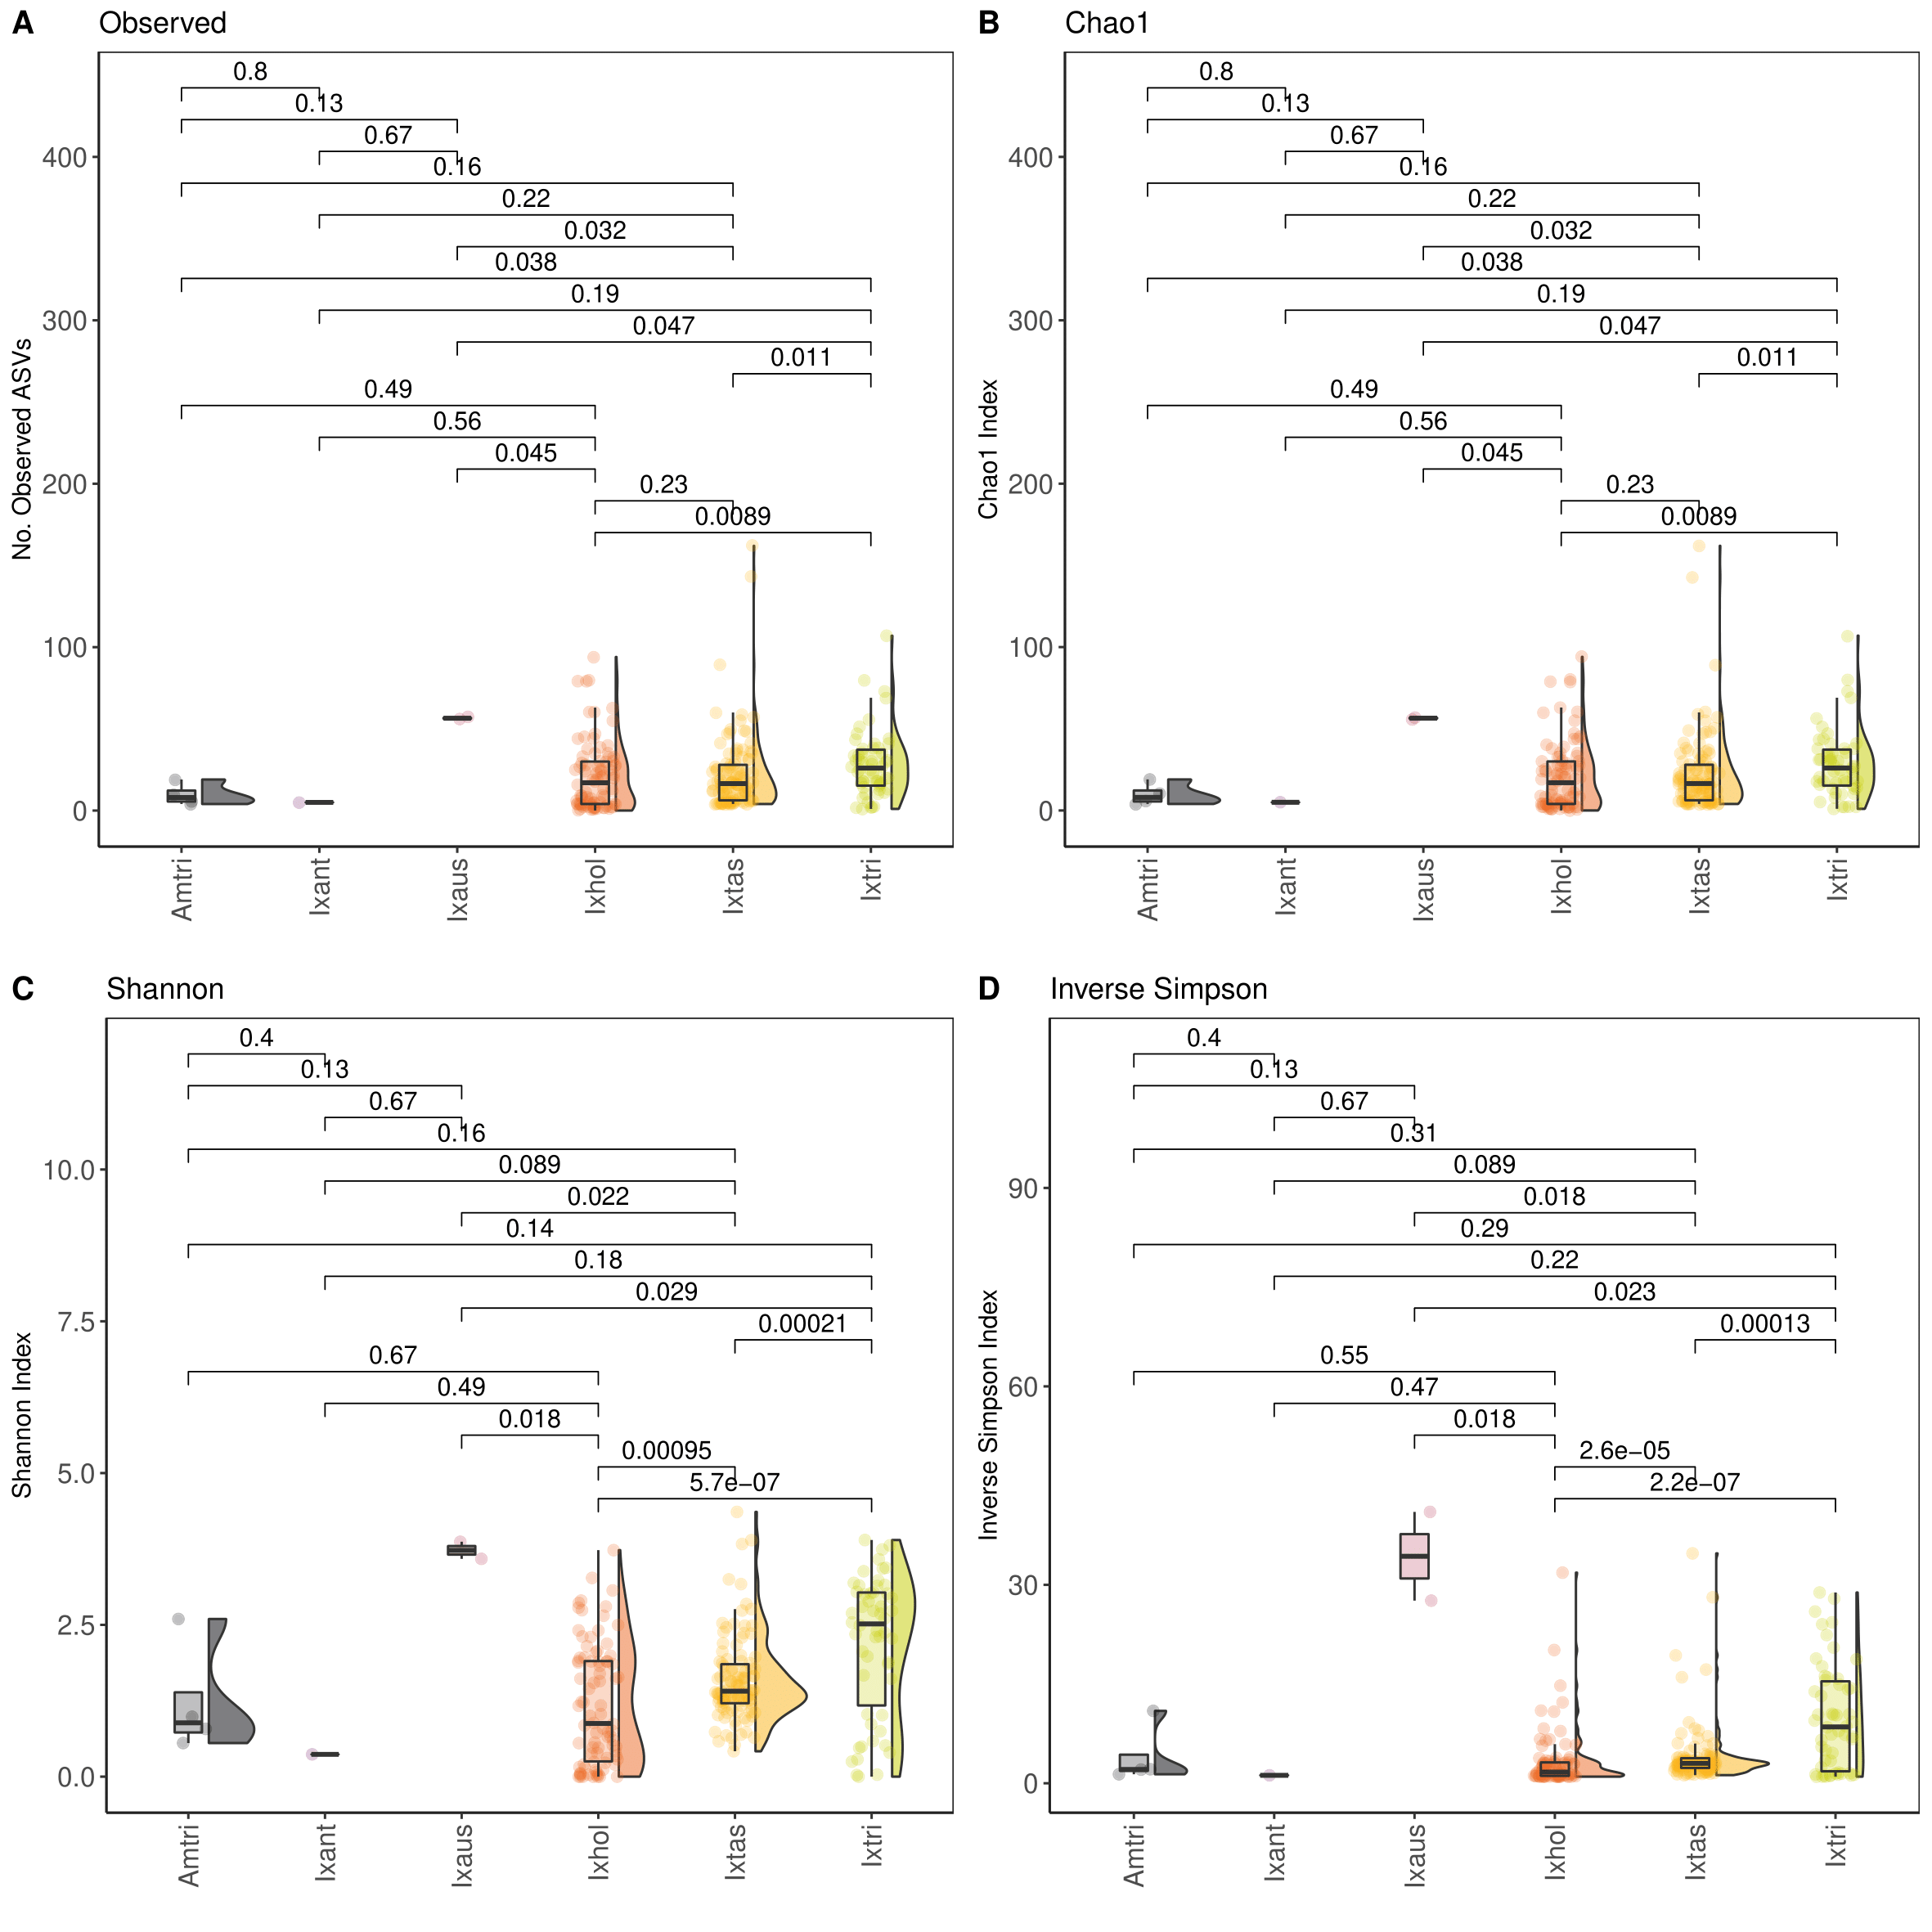
\includegraphics[width=0.95\linewidth]{figures/ms-figs-appendix/FigA-3.3} \caption[Alpha diversity of microbiome community for tick samples.]{Boxplot of Alpha-diversity indices for tick samples. Diversity indexes (A) Observed number of ASVs, (B) Chao1 index, (C) Shannon index and (D) inverse Simpson index. Boxplots and violin plots represent the distribution of diversity among tick species. Statistical analysis between sample types calculated using Wilcoxon pairwise (non-parametric) test. Pools of different tick species excluded from analysis.}\label{fig:FA33}
\end{figure}

\newpage

\begin{figure}
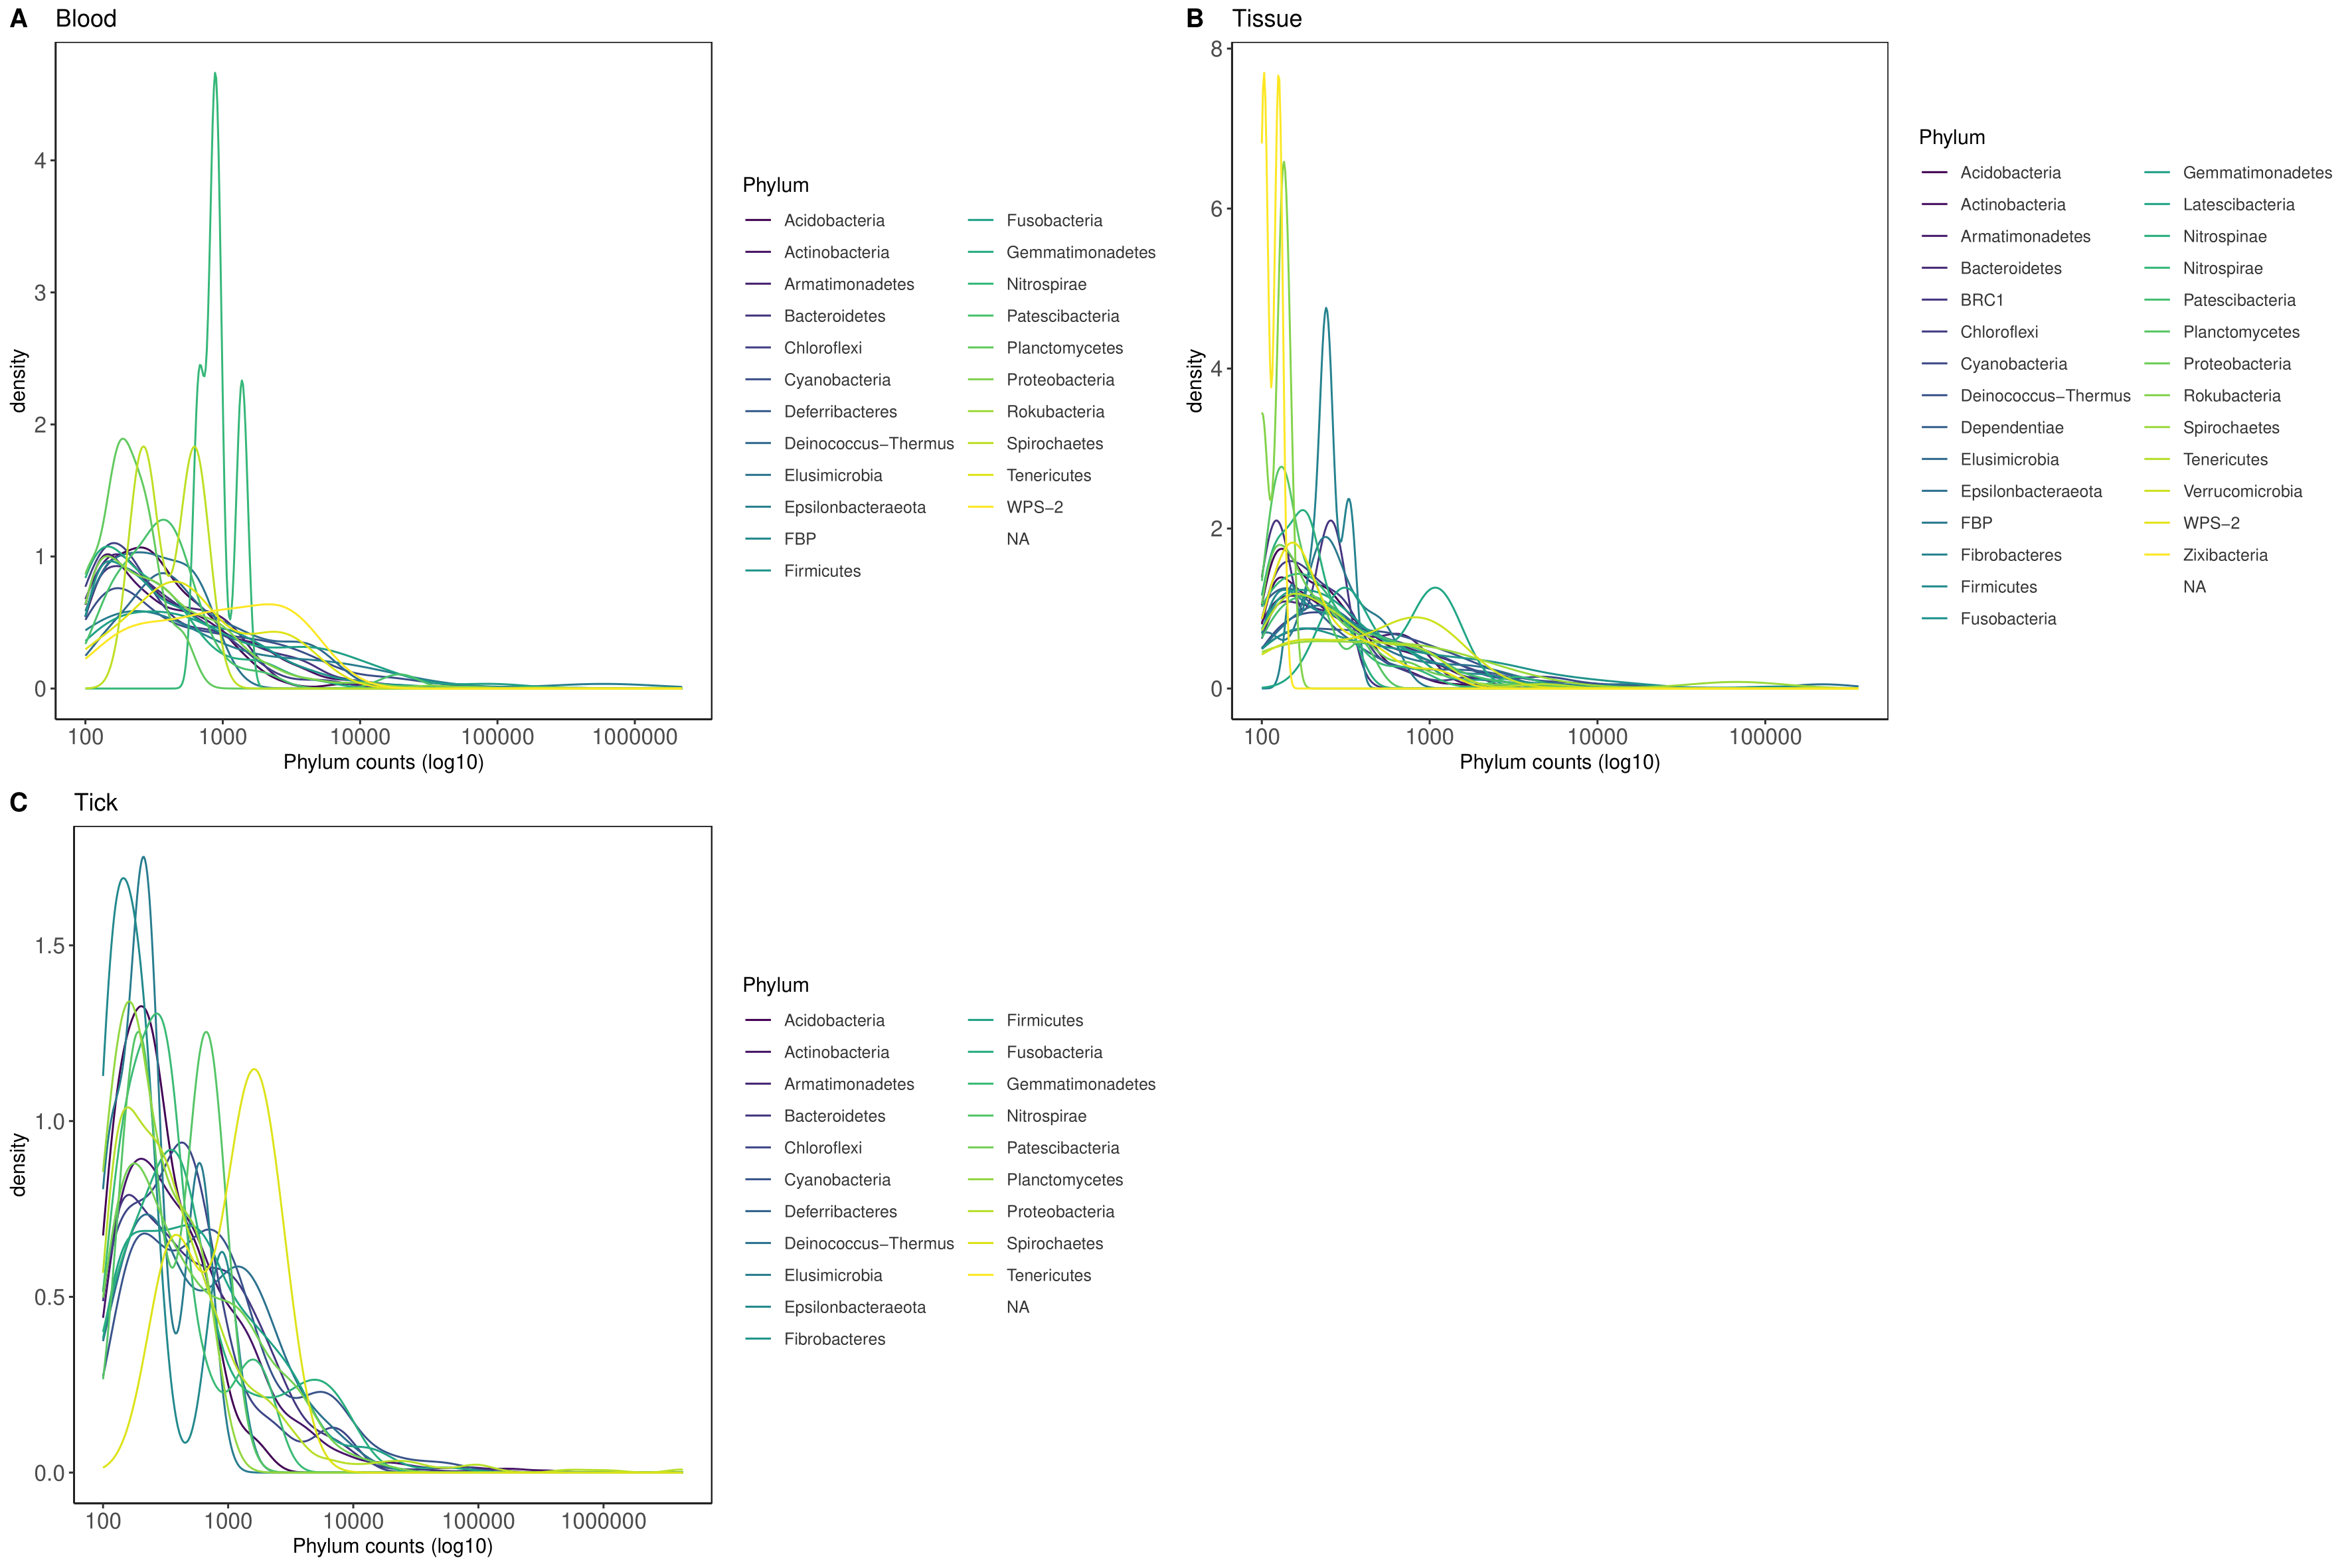
\includegraphics[width=0.95\linewidth]{figures/ms-figs-appendix/FigA-3.4} \caption[Phylum level distribution plots.]{Phylum level distribution plots of bacterial composition in wildlife samples.}\label{fig:FA34}
\end{figure}

\newpage

\begin{figure}
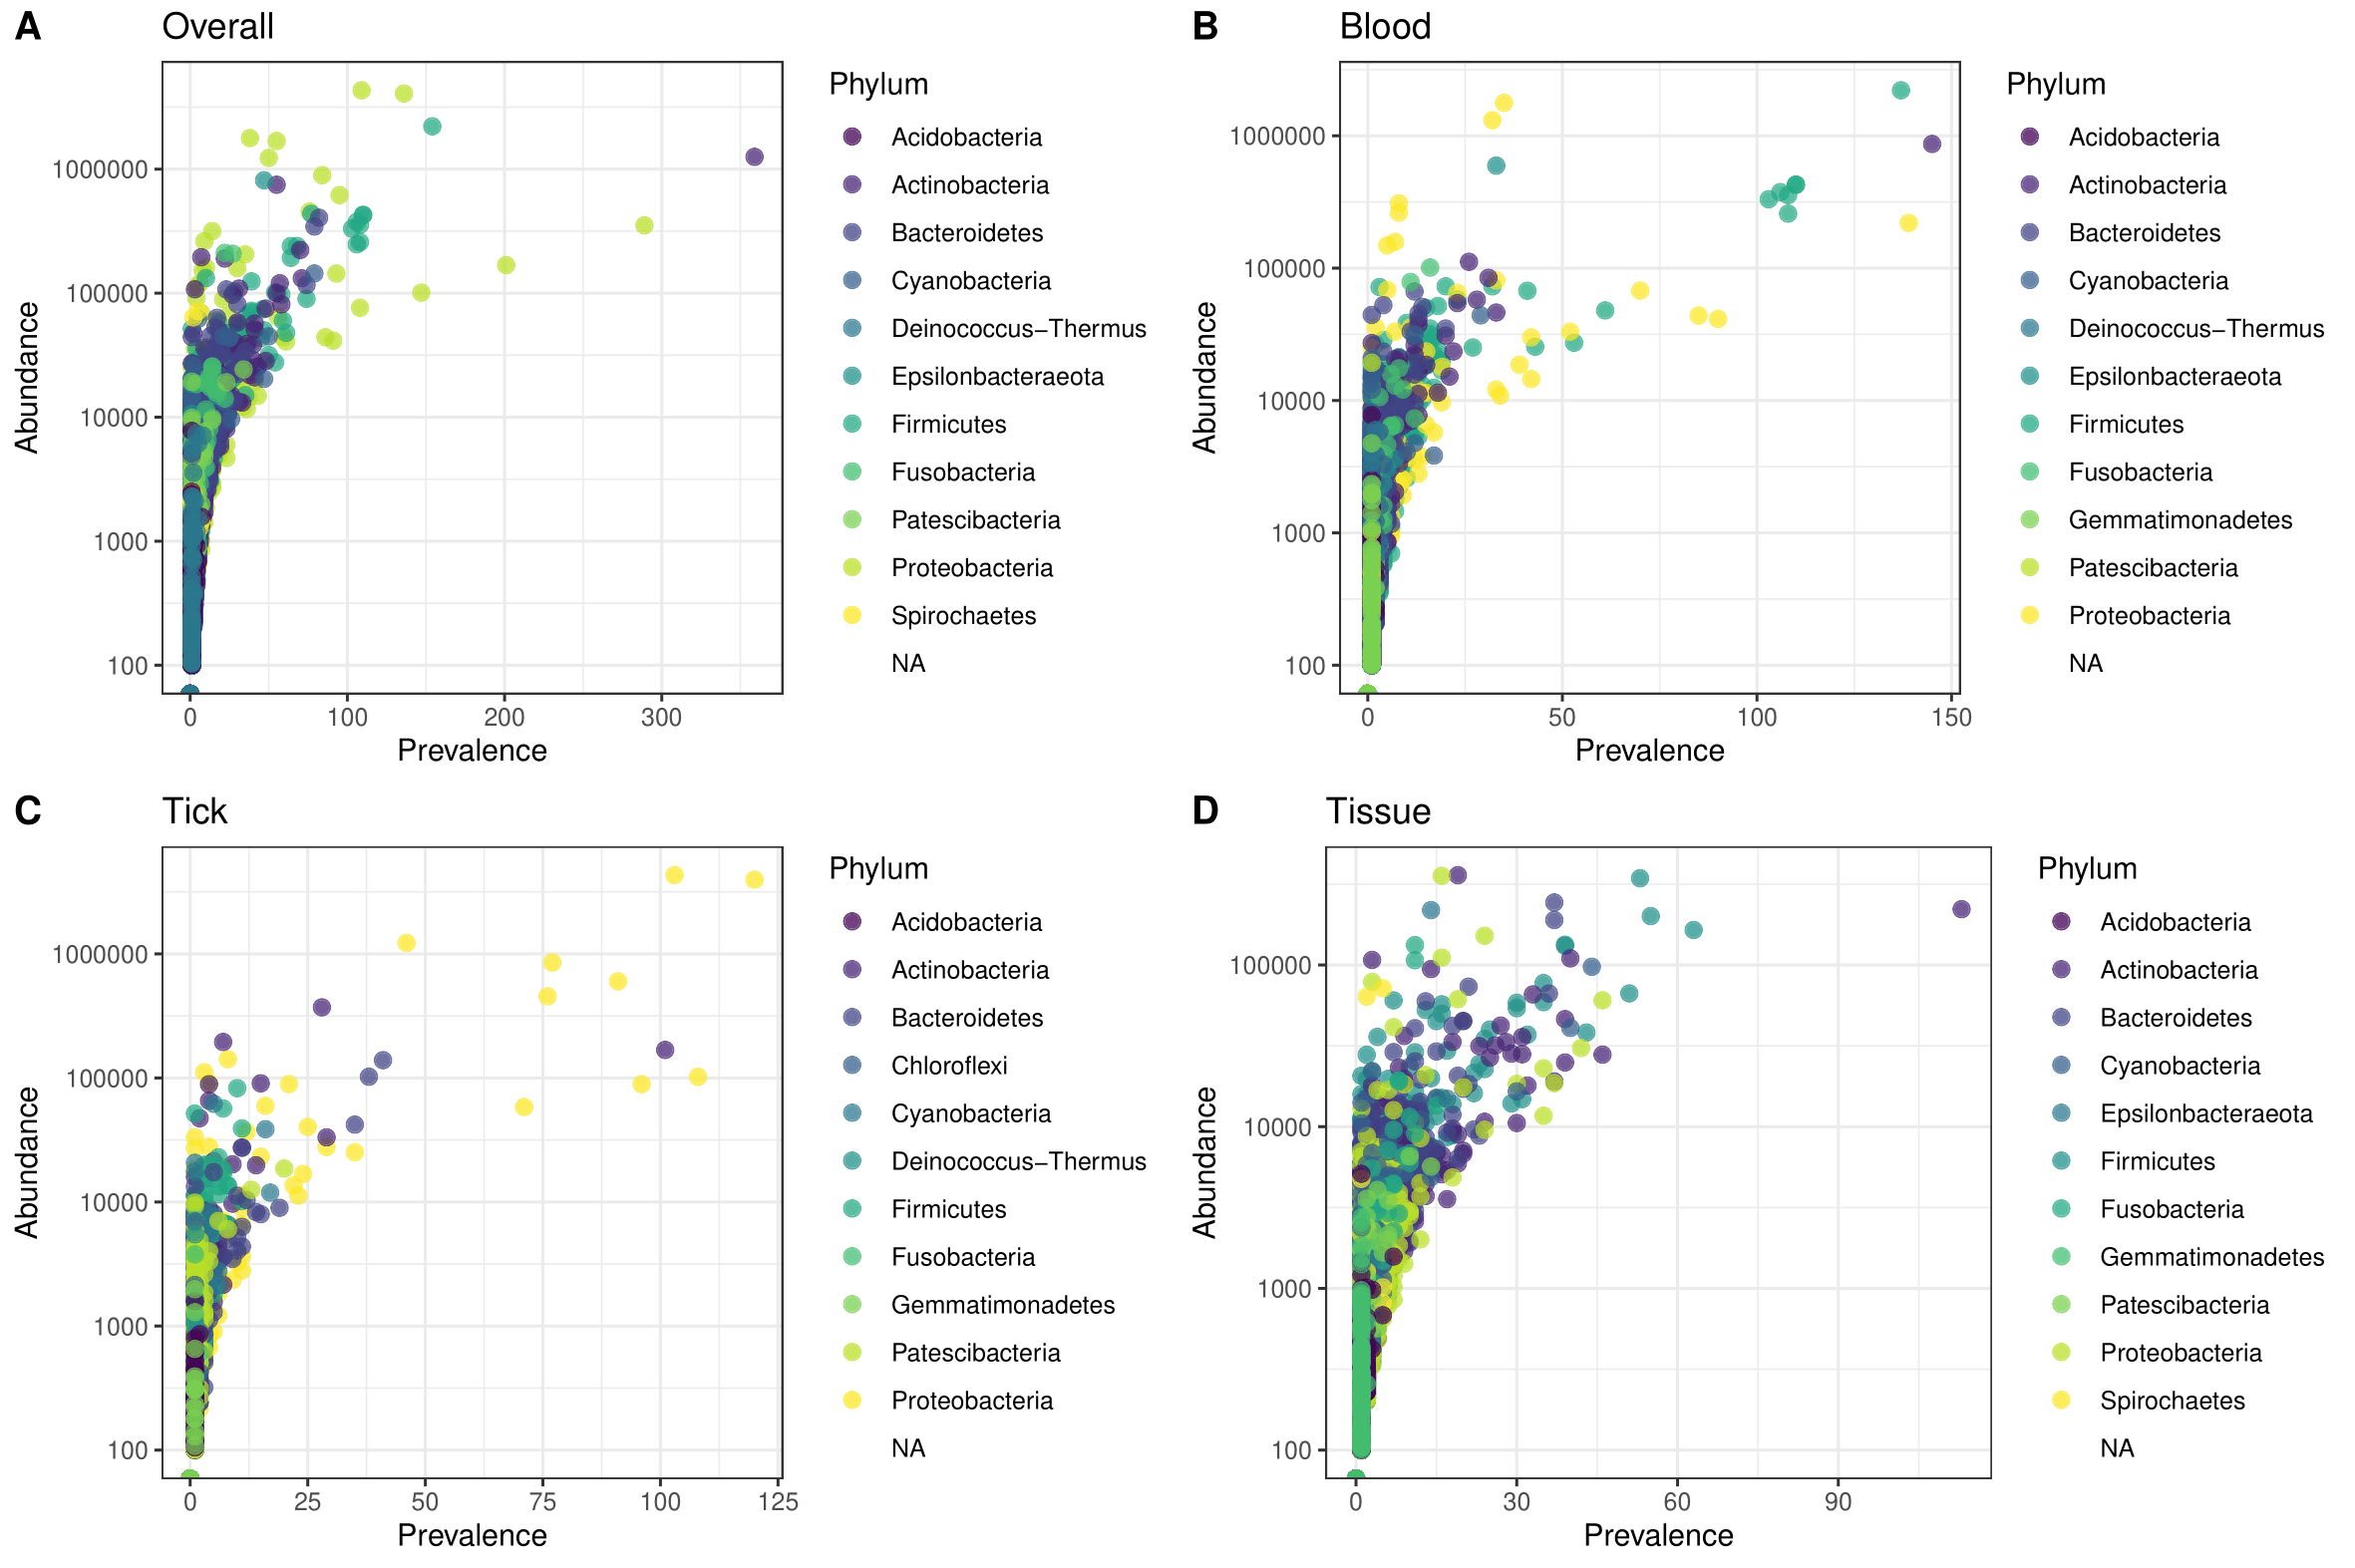
\includegraphics[width=0.95\linewidth]{figures/ms-figs-appendix/FigA-3.5} \caption[Phylum level taxa abundance.]{Abundance (no. of sequences) and prevalence in samples of bacterial phyla identified from wildlife samples (A) overall, (B) blood, (C) tick and (D) tissue.}\label{fig:FA35}
\end{figure}

\newpage

\begin{figure}
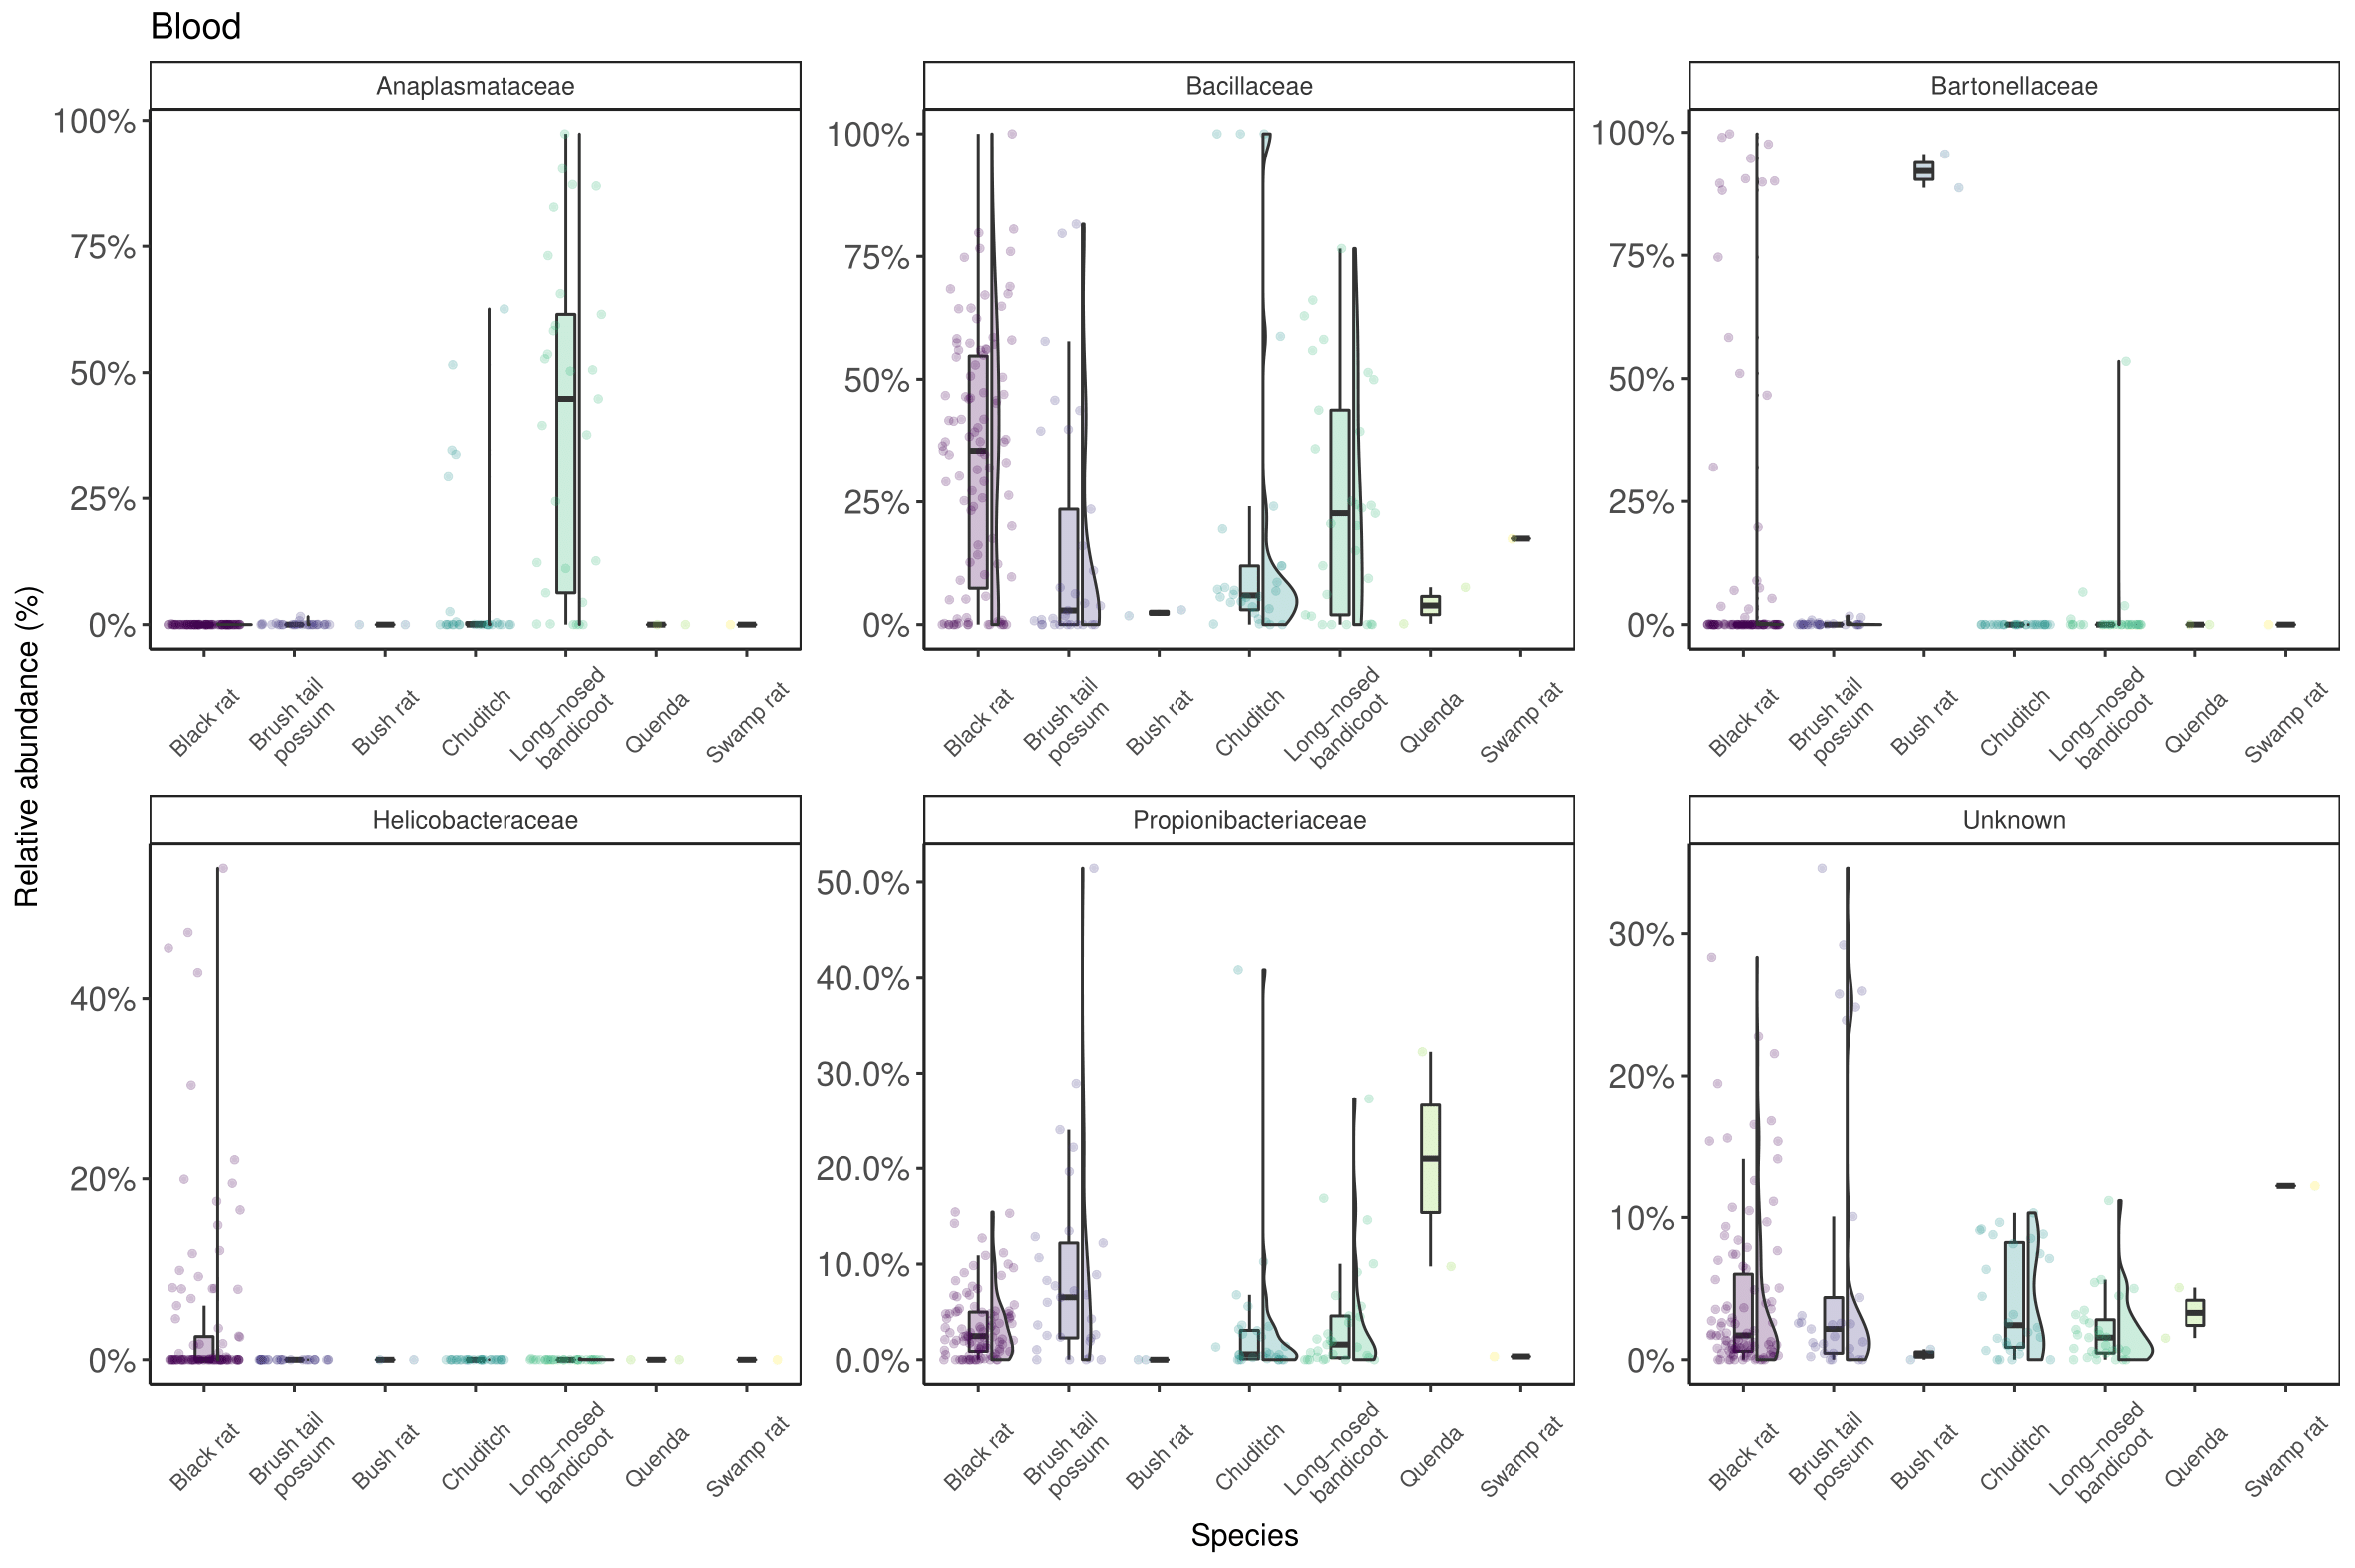
\includegraphics[width=0.8\linewidth]{figures/ms-figs-appendix/FigA-3.6} \caption[Bacterial family taxa identified in wildlife blood samples.]{Bacterial family taxa (top 6 most abundant) identified in wildlife blood samples.}\label{fig:FA36}
\end{figure}

\newpage

\begin{figure}
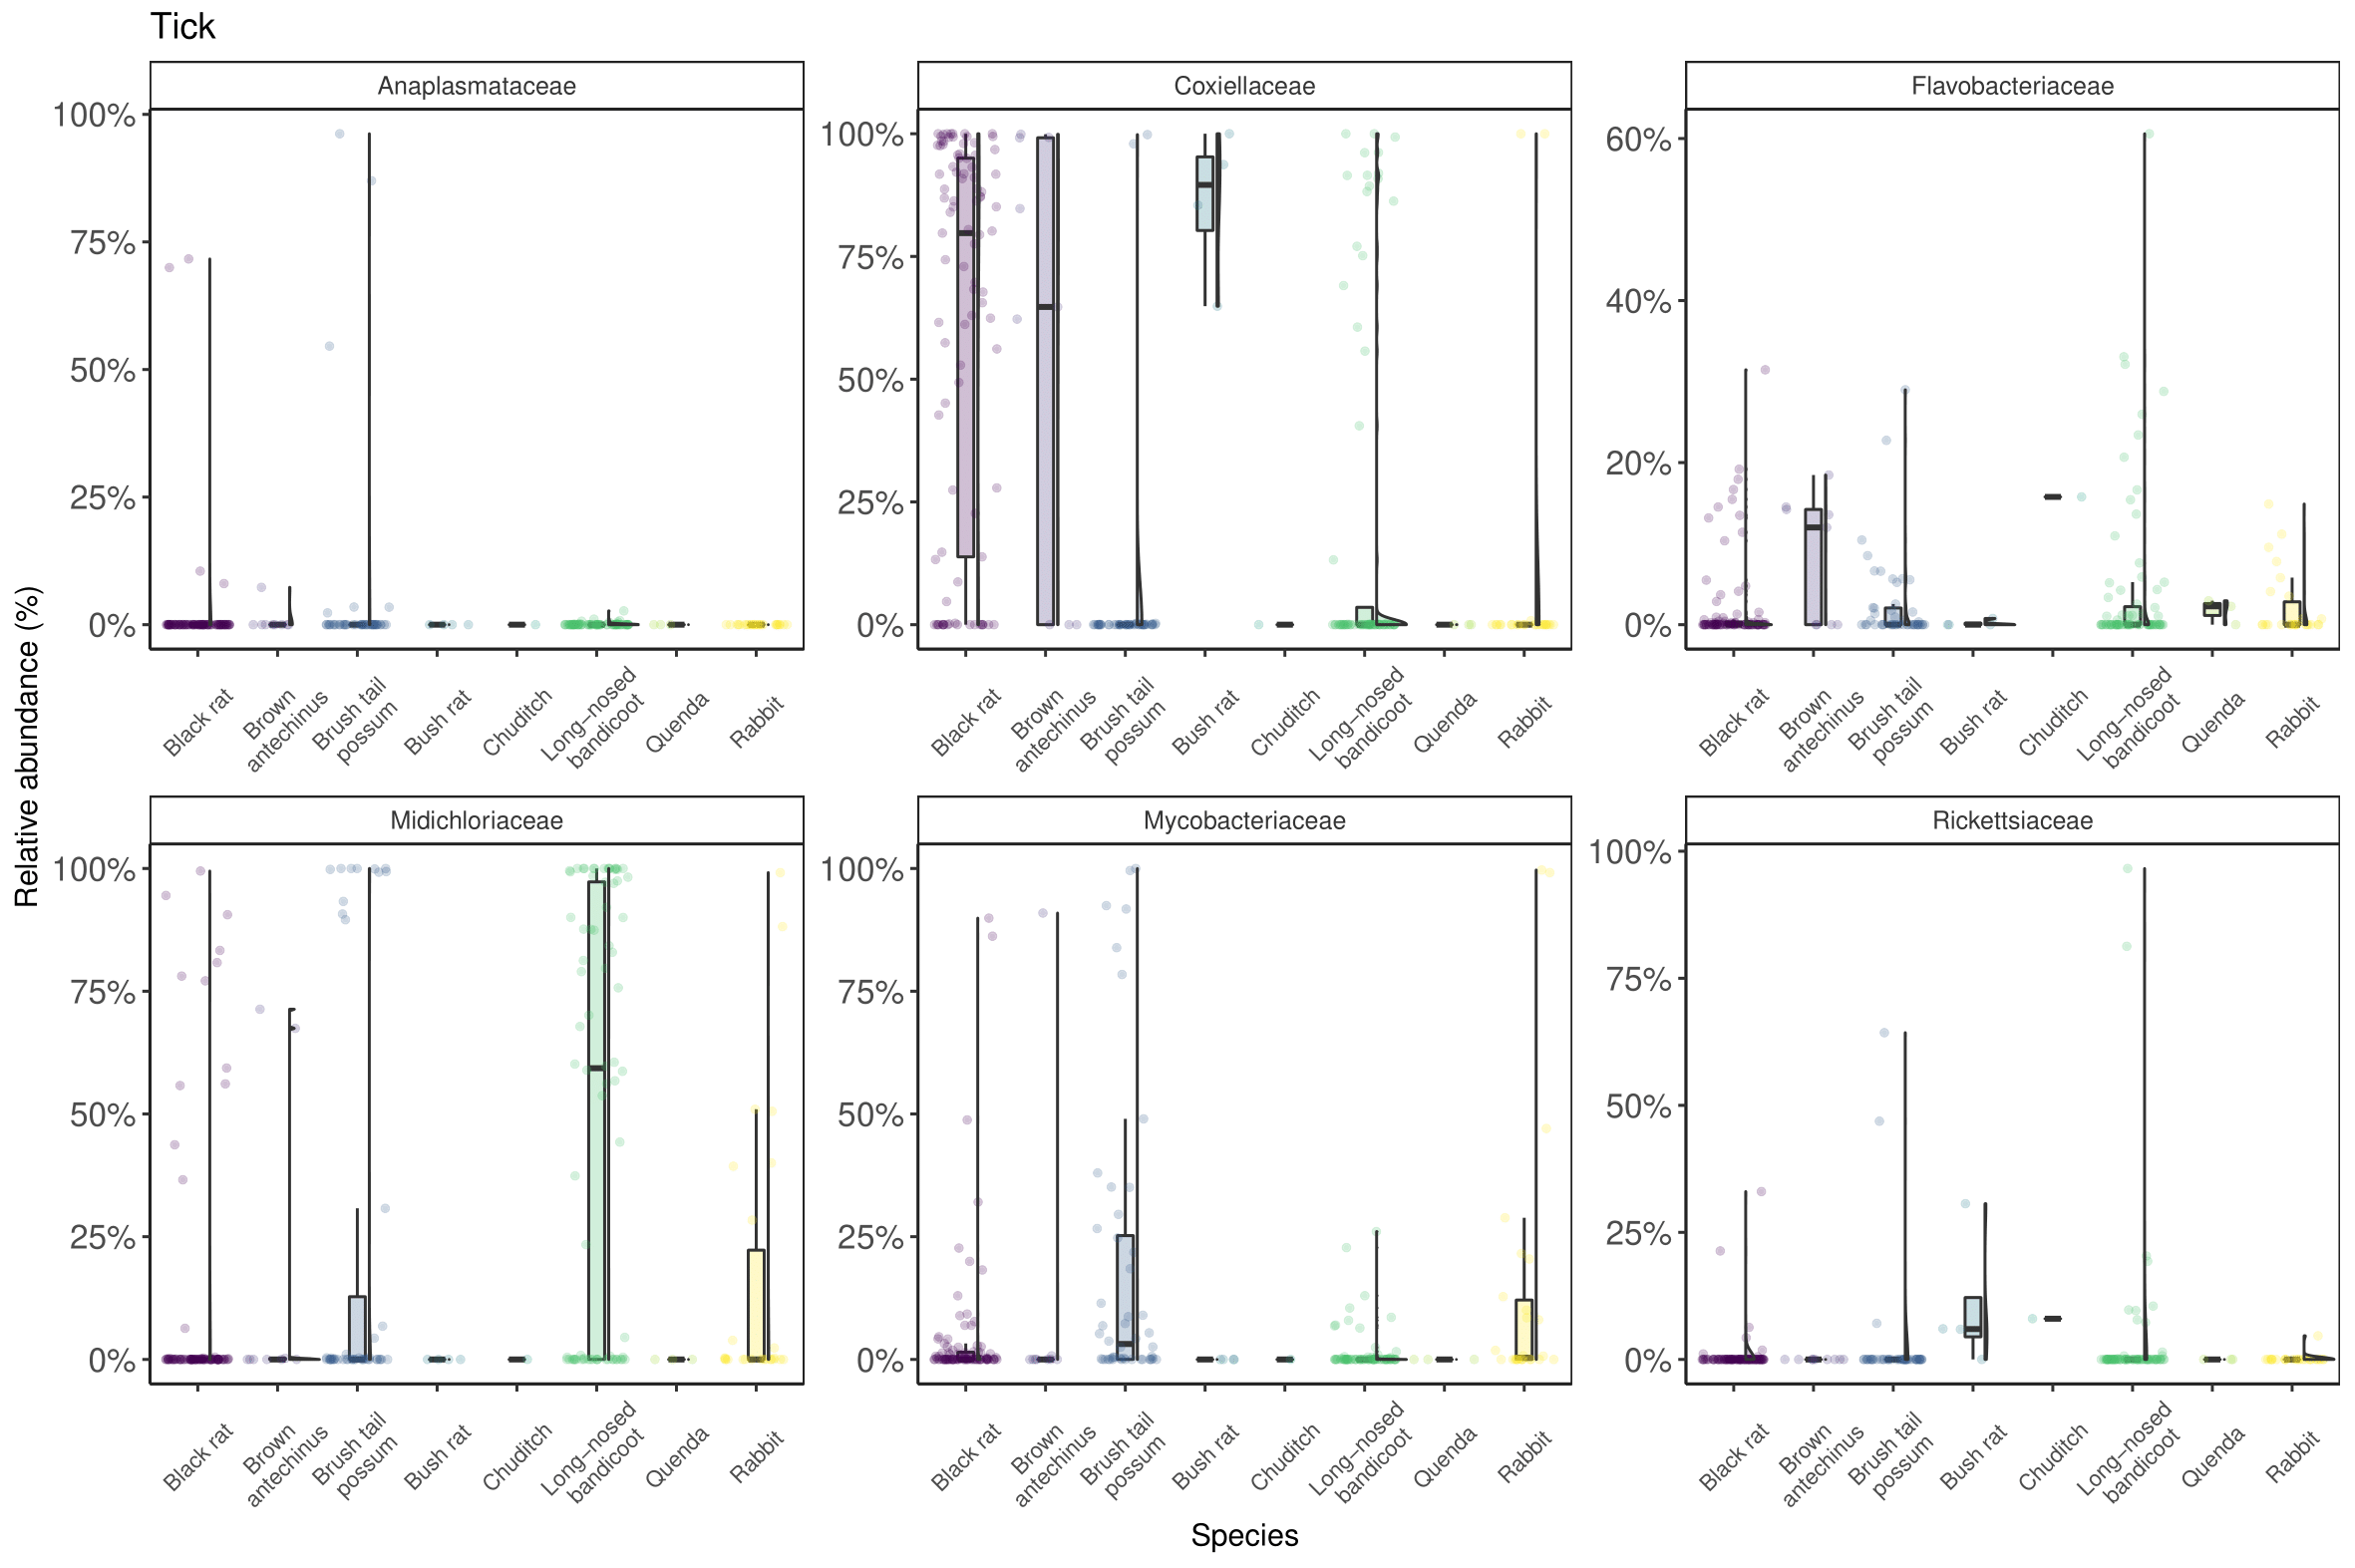
\includegraphics[width=0.8\linewidth]{figures/ms-figs-appendix/FigA-3.7} \caption[Bacterial family taxa identified in wildlife tick samples.]{Bacterial family taxa (top 6 most abundant) identified in wildlife tick samples.}\label{fig:FA37}
\end{figure}

\newpage

\begin{figure}
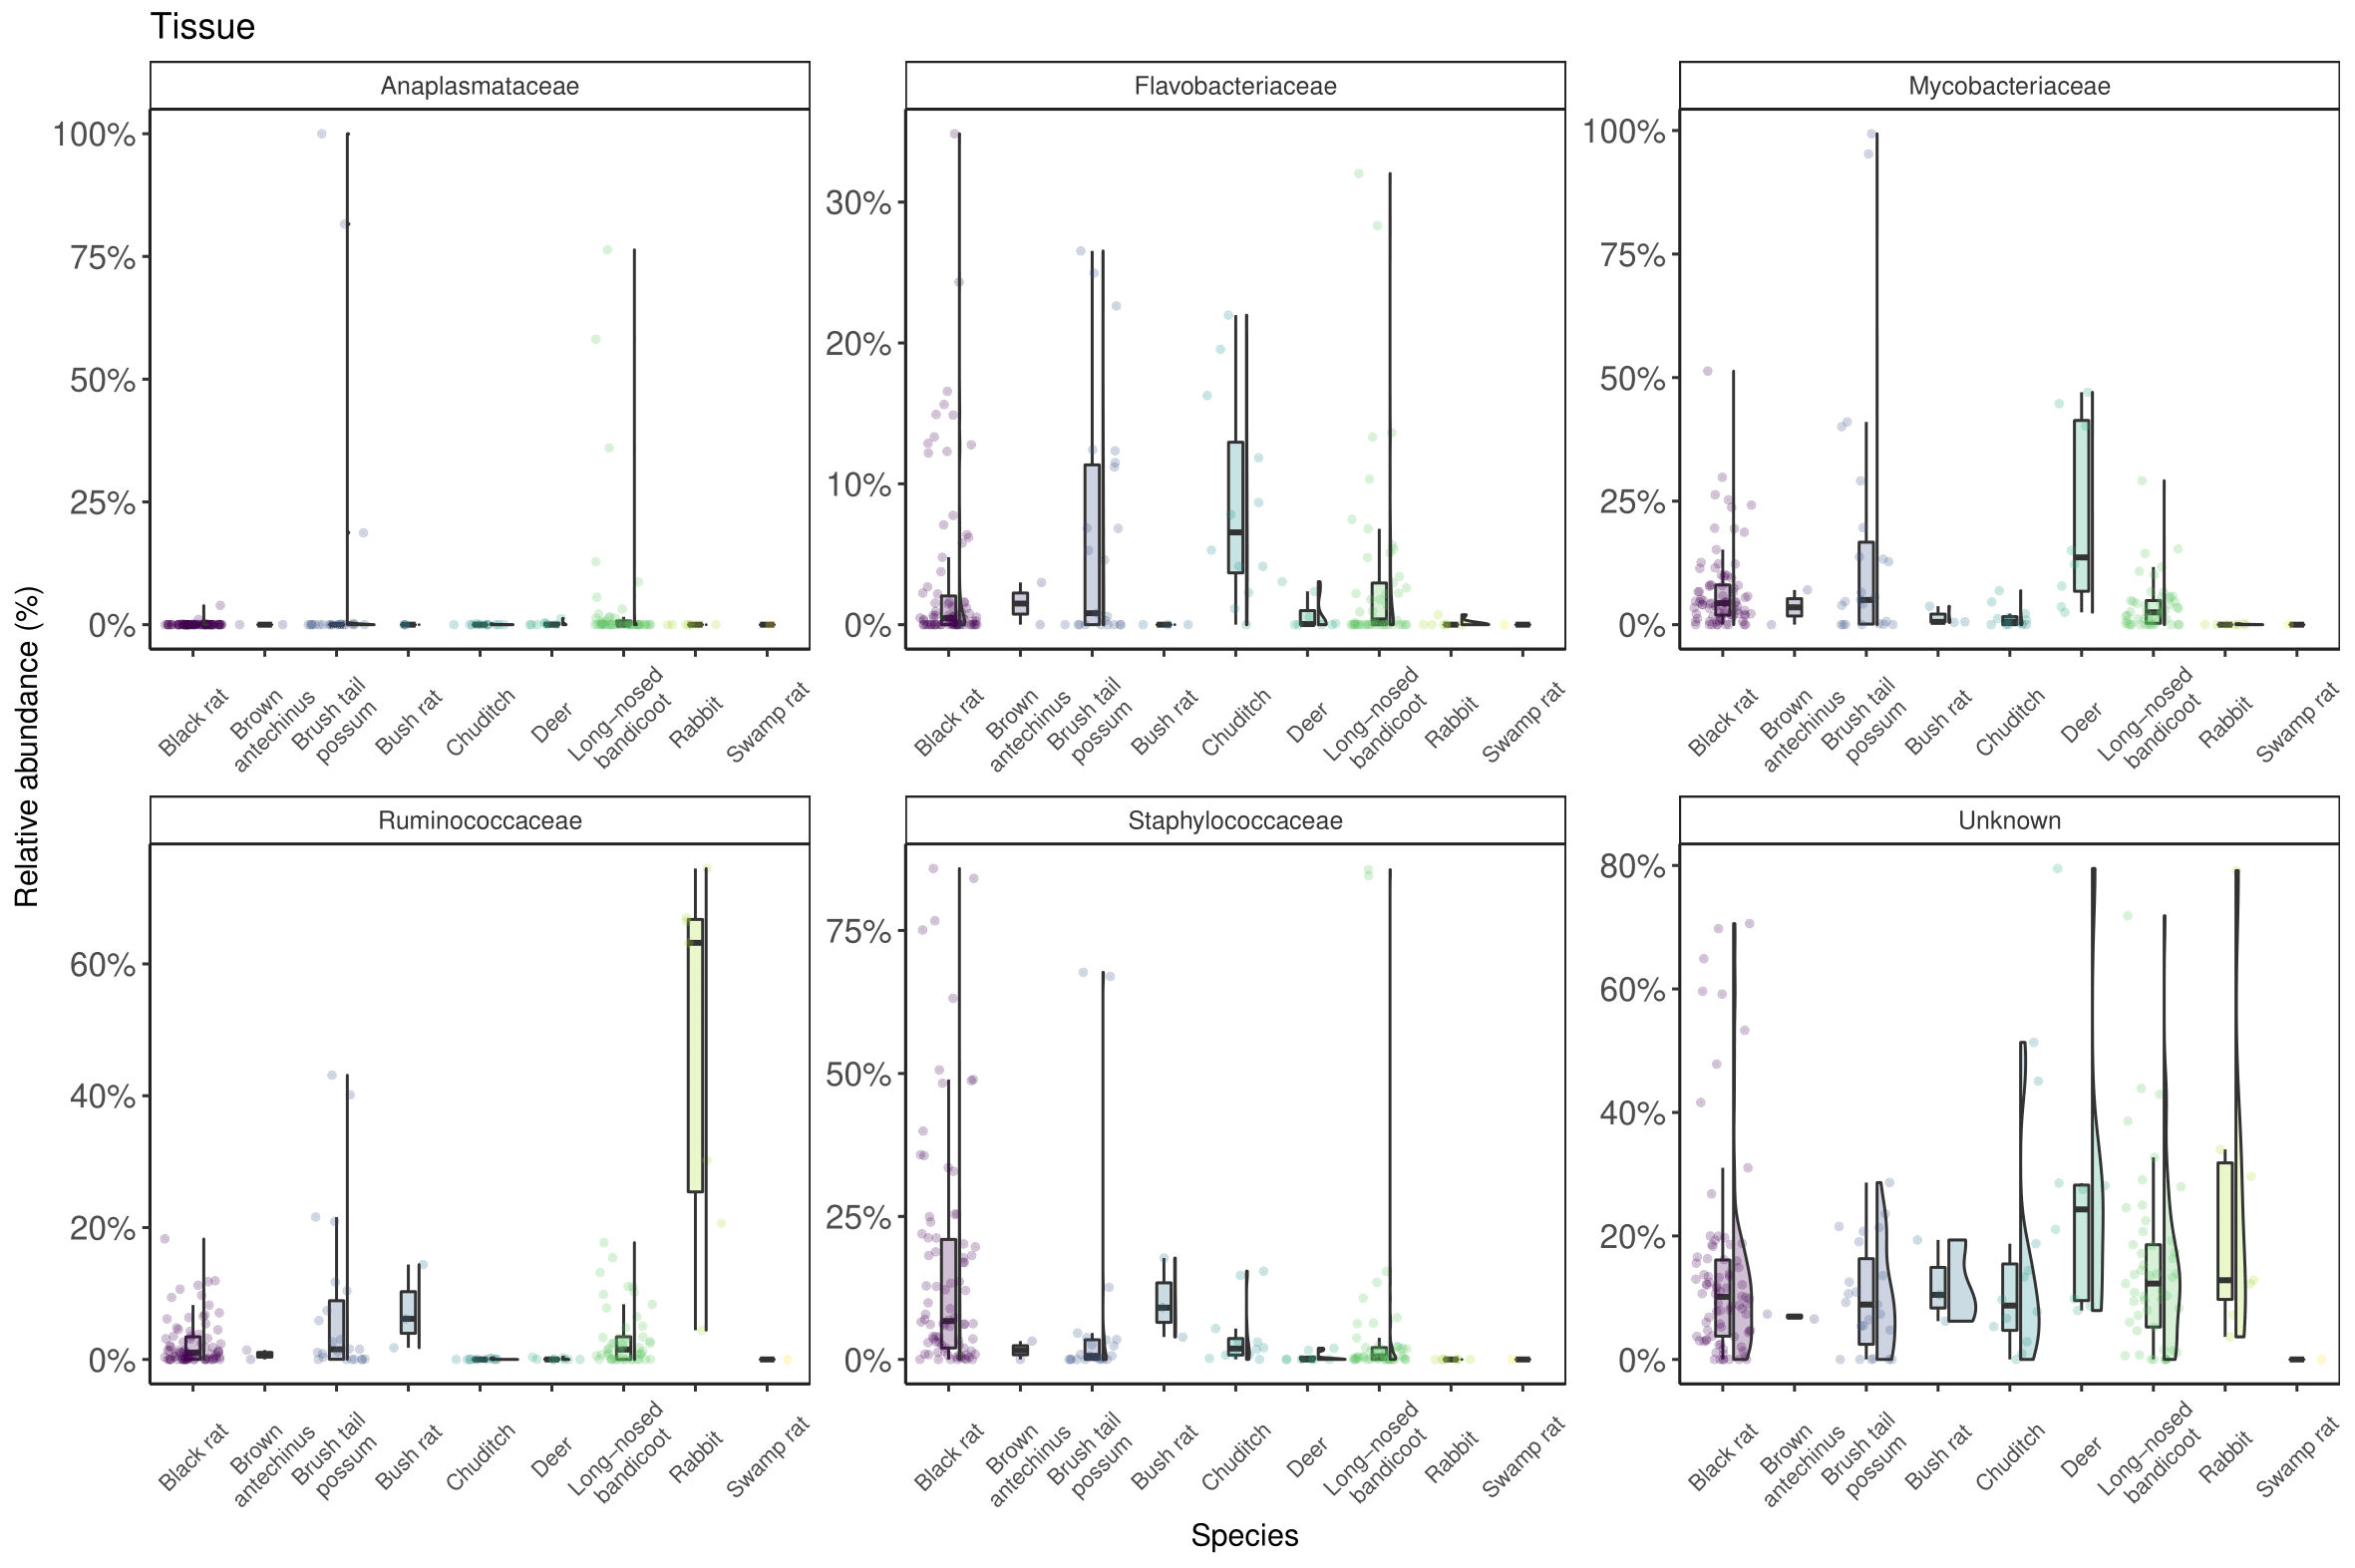
\includegraphics[width=0.8\linewidth]{figures/ms-figs-appendix/FigA-3.8} \caption[Bacterial family taxa identified in wildlife tissue samples.]{Bacterial family taxa (top 6 most abundant) identified in wildlife tissue samples.}\label{fig:FA38}
\end{figure}

\newpage

\begin{figure}
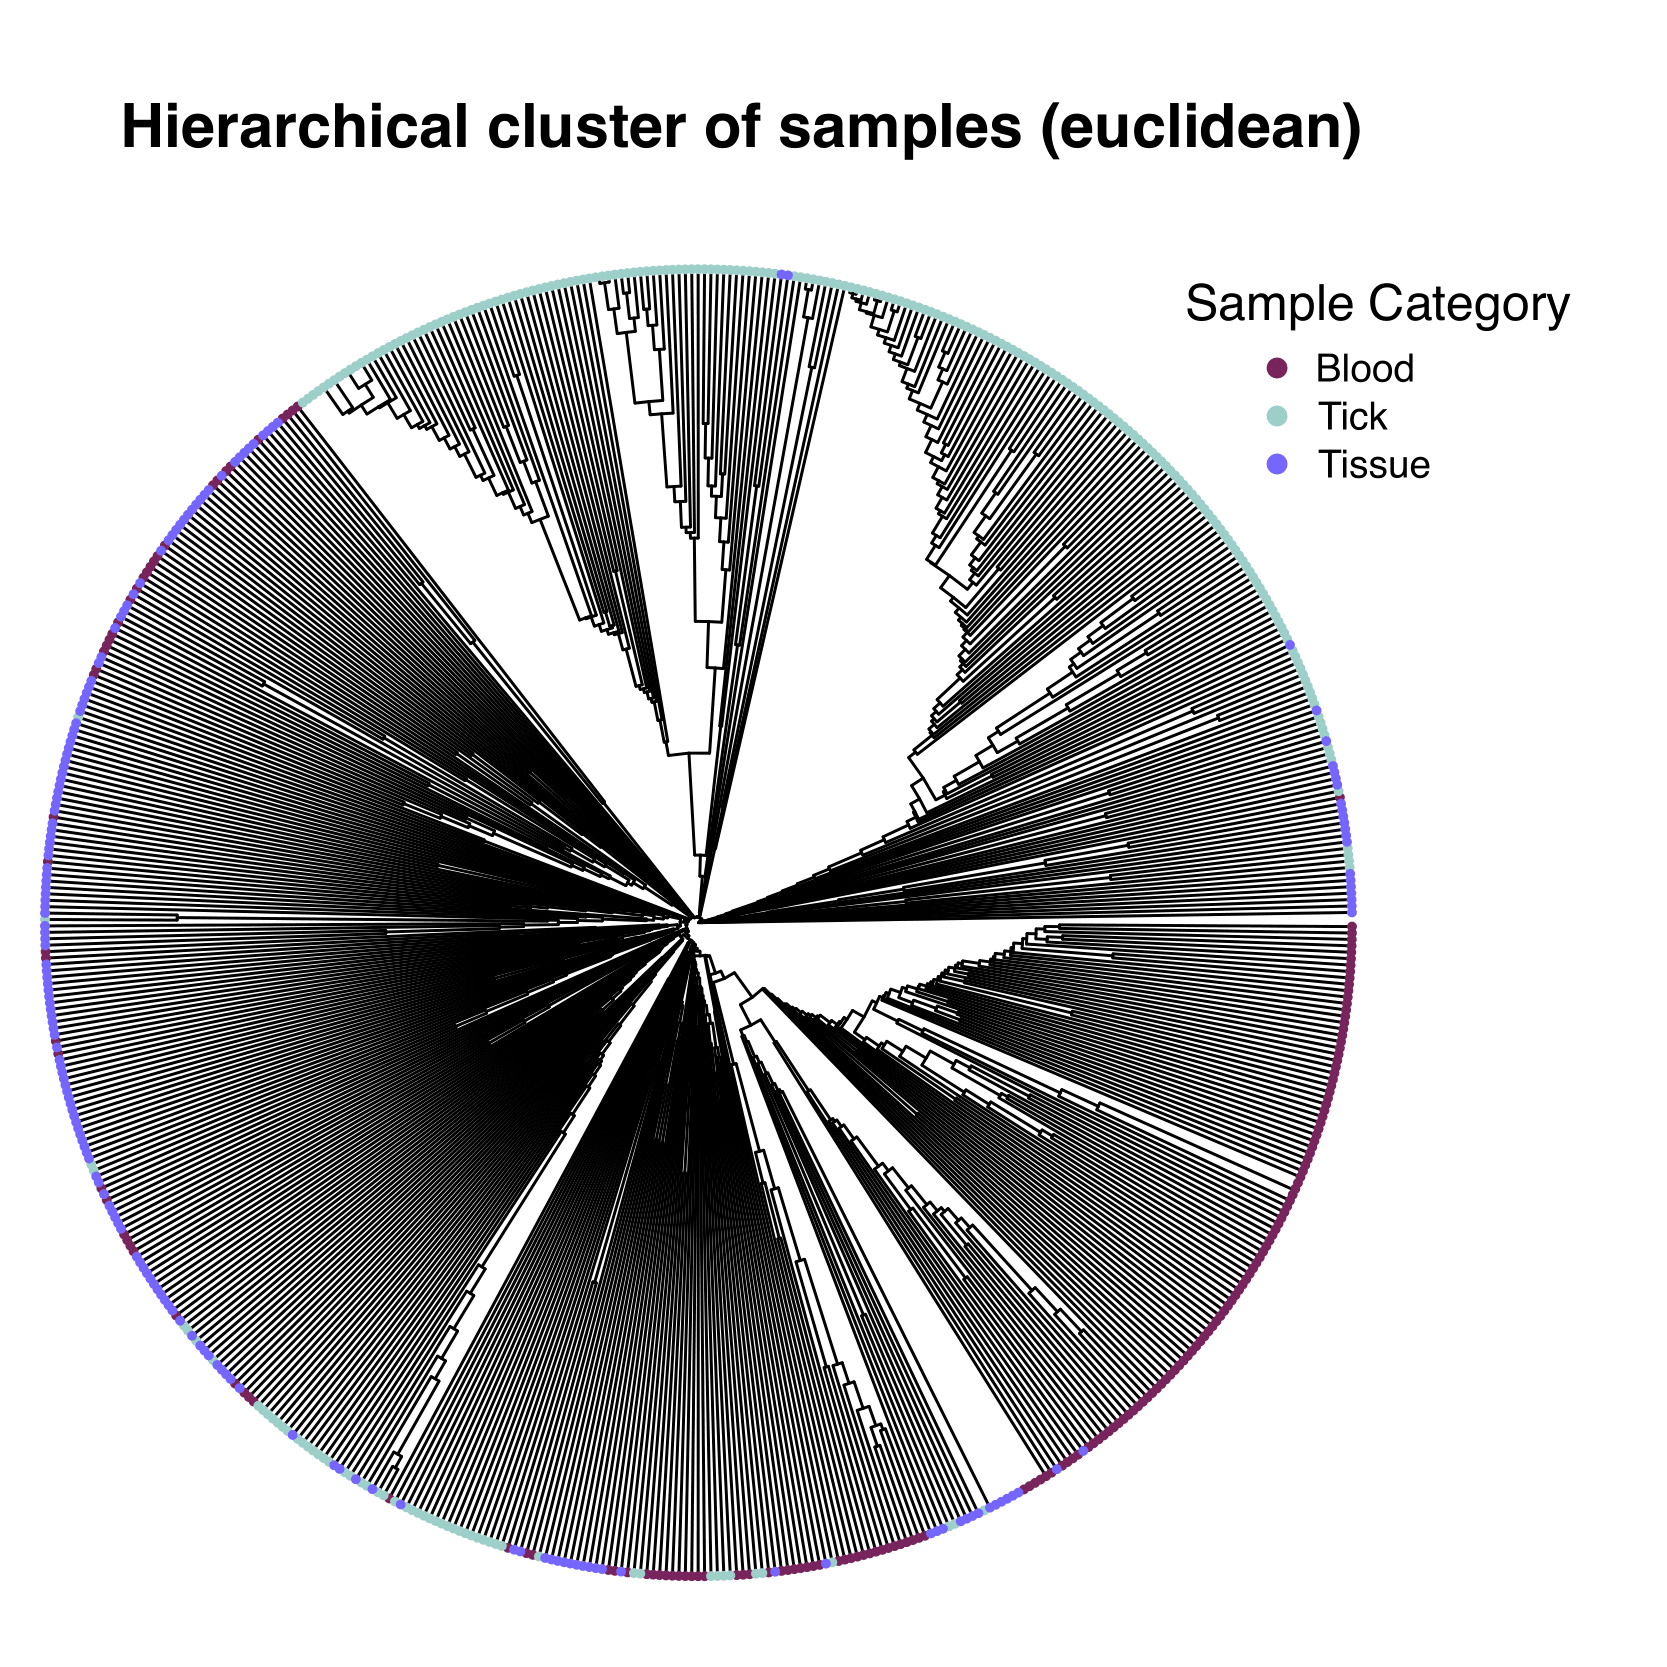
\includegraphics[width=0.95\linewidth]{figures/ms-figs-appendix/FigA-3.9} \caption[Hierarchical cluster analysis of bacterial communities - all samples.]{Hierarchical cluster analysis of bacterial communities from wildlife samples. Data points coloured by sample type; blood, tick and tissue. Cluster analysis was performed using euclidean distance measure (average), data was transformed using Hellinger transformation.}\label{fig:FA39}
\end{figure}

\newpage

\begin{figure}
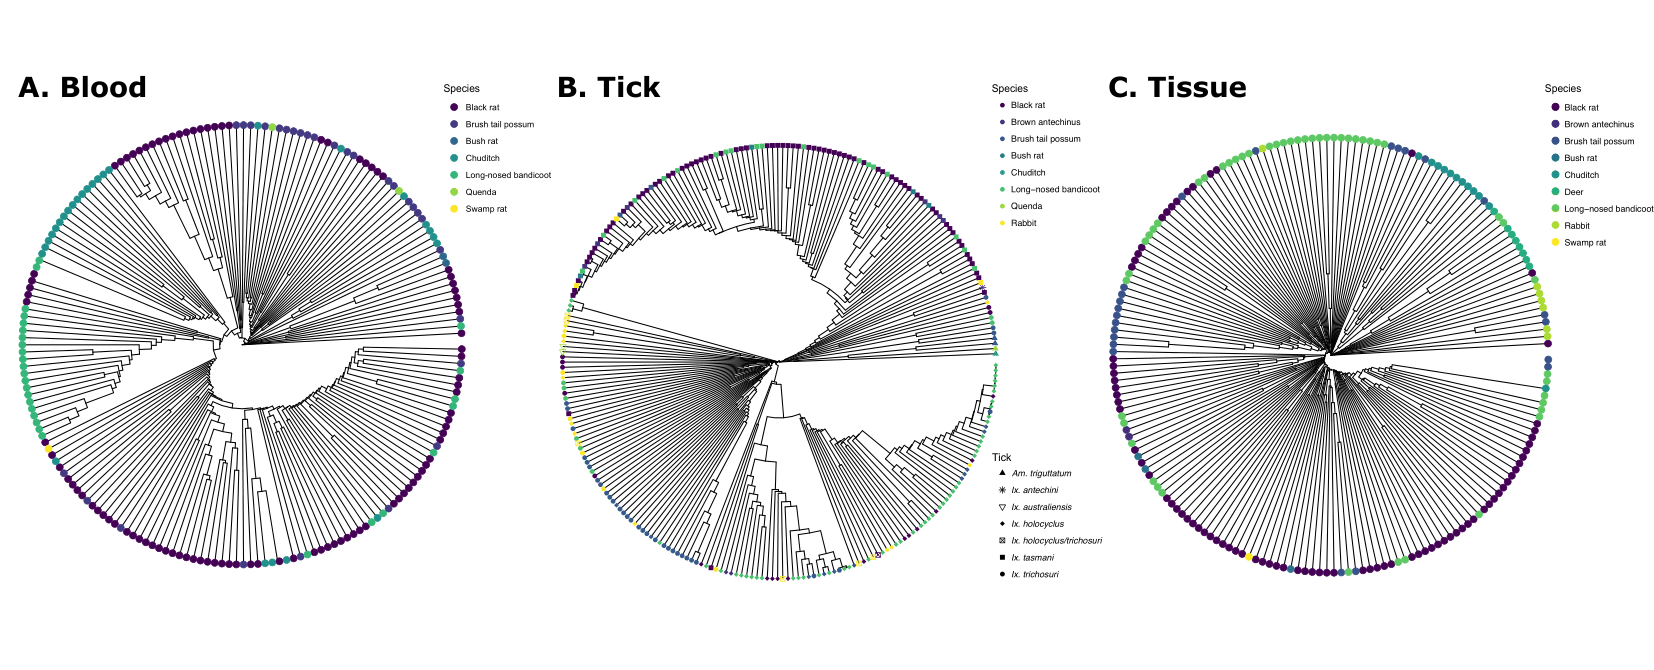
\includegraphics[width=0.95\linewidth]{figures/ms-figs-appendix/FigA-3.10} \caption[Hierarchical cluster analysis of bacterial communities - by sample type.]{Hierarchical cluster analysis of bacterial communities from wildlife samples, separated by sample types. (A) Blood, (B) Tick, (C) Tissue. Data points coloured by host species (and tick species (B)). Cluster analysis was performed using euclidean distance measure (average), data was transformed using Hellinger transformation.}\label{fig:FA310}
\end{figure}

\clearpage

\hypertarget{ch3stats}{%
\subsection{Statistical analysis}\label{ch3stats}}

Beta diversity statistical analysis of bacterial microbiome composition using analysis of variance (ANOVA) and permutational multivariate analysis of variance (PERMANOVA) methods.
Statistical analysis calculated using the vegan R package.
Data cleaning and transformation: removed samples with \textless{} 1000 sequences, transformed data using Hellinger transformation method. Distance calculated using Bray-Curtis distance measure.

\hypertarget{ch3stats1}{%
\subsubsection{Sample Type}\label{ch3stats1}}

Statistical analysis comparing the bacterial microbiome of blood, tick and tissue samples collected form wildlife.

\emph{A. Analysis of Variance (ANOVA)}

\begin{verbatim}
Analysis of Variance Table

Response: Distances
           Df Sum Sq  Mean Sq F value    Pr(>F)    
Groups      2 0.4466 0.223289  36.209 1.364e-15 ***
Residuals 614 3.7863 0.006167                      
---
Signif. codes:  0 ‘***’ 0.001 ‘**’ 0.01 ‘*’ 0.05 ‘.’ 0.1 ‘ ’ 1
\end{verbatim}

\emph{B. Permutational multivariate analysis of variance (PERMANOVA)}

\begin{verbatim}
Permutation test for homogeneity of multivariate dispersions
Permutation: free
Number of permutations: 999

Response: Distances
           Df Sum Sq  Mean Sq      F N.Perm Pr(>F)    
Groups      2 0.4466 0.223289 36.209    999  0.001 ***
Residuals 614 3.7863 0.006167                         
---
Signif. codes:  0 ‘***’ 0.001 ‘**’ 0.01 ‘*’ 0.05 ‘.’ 0.1 ‘ ’ 1

Pairwise comparisons:
(Observed p-value below diagonal, permuted p-value above diagonal)
            Blood       Tick Tissue
Blood             4.1600e-01  0.001
Tick   4.0839e-01             0.001
Tissue 8.8347e-17 3.5464e-15       
\end{verbatim}

\newpage

\hypertarget{ch3stats2}{%
\subsubsection{Tick species}\label{ch3stats2}}

Statistical analysis comparing bacterial microbiome of tick collected from wildlife (all tick species).

\emph{A. Analysis of Variance (ANOVA)}

\begin{verbatim}
Analysis of Variance Table

Response: Distances
           Df Sum Sq Mean Sq F value    Pr(>F)    
Groups      6 2.5929 0.43215   14.01 9.594e-14 ***
Residuals 251 7.7423 0.03085         
\end{verbatim}

\emph{B. Permutational multivariate analysis of variance (PERMANOVA)}

\begin{verbatim}
Permutation test for homogeneity of multivariate dispersions
Permutation: free
Number of permutations: 999

Response: Distances
           Df Sum Sq Mean Sq     F N.Perm Pr(>F)    
Groups      6 2.5929 0.43215 14.01    999  0.001 ***
Residuals 251 7.7423 0.03085                        
---
Signif. codes:  0 ‘***’ 0.001 ‘**’ 0.01 ‘*’ 0.05 ‘.’ 0.1 ‘ ’ 1

Pairwise comparisons:
(Observed p-value below diagonal, permuted p-value above diagonal)
                 Amtri Ixant      Ixaus      Ixhol Ixhol;Ixtri      Ixtas Ixtri
Amtri                        9.4400e-01 3.6500e-01  2.5700e-01 7.8500e-01 0.001
Ixant                                                                          
Ixaus       9.3797e-01                  5.9300e-01  3.8000e-02 7.3300e-01 0.001
Ixhol       3.4424e-01       5.7323e-01             5.3700e-01 1.0000e-03 0.001
Ixhol;Ixtri 2.4249e-01       4.5601e-02 5.3705e-01             3.8000e-02 0.001
Ixtas       7.8073e-01       7.4761e-01 3.5985e-05  3.8405e-02            0.001
Ixtri       1.0858e-06       4.6854e-09 2.0461e-06  1.2151e-05 5.1524e-15   
\end{verbatim}

\newpage

Statistical analysis comparing bacterial microbiome of cohabiting tick species collected from wildlife in Sydney Northern Beaches area, New South Wales (\emph{Ix. holocyclus}, \emph{Ix. tasmani}, and \emph{Ix. trichosuri}).

\emph{A. Analysis of Variance (ANOVA)}

\begin{verbatim}
Analysis of Variance Table

Response: Distances
           Df Sum Sq Mean Sq F value    Pr(>F)    
Groups      3 2.3202 0.77341  25.465 2.177e-14 ***
Residuals 247 7.5019 0.03037                      
---
Signif. codes:  0 ‘***’ 0.001 ‘**’ 0.01 ‘*’ 0.05 ‘.’ 0.1 ‘ ’ 1
\end{verbatim}

\emph{B. Permutational multivariate analysis of variance (PERMANOVA)}

\begin{verbatim}
Permutation test for homogeneity of multivariate dispersions
Permutation: free
Number of permutations: 999

Response: Distances
           Df Sum Sq Mean Sq      F N.Perm Pr(>F)    
Groups      3 2.3202 0.77341 25.465    999  0.001 ***
Residuals 247 7.5019 0.03037                         
---
Signif. codes:  0 ‘***’ 0.001 ‘**’ 0.01 ‘*’ 0.05 ‘.’ 0.1 ‘ ’ 1

Pairwise comparisons:
(Observed p-value below diagonal, permuted p-value above diagonal)
                 Ixhol Ixhol;Ixtri      Ixtas Ixtri
Ixhol                   5.3000e-01 1.0000e-03 0.001
Ixhol;Ixtri 5.3687e-01             3.9000e-02 0.001
Ixtas       3.5862e-05  3.8383e-02            0.001
Ixtri       2.0485e-06  1.2237e-05 5.1829e-15     
\end{verbatim}

\clearpage

\hypertarget{ch3-esupp}{%
\subsection{Supplementary Electronic Tables}\label{ch3-esupp}}

The following electronic supplementary files are available for download on \href{https://figshare.com/s/0f5495957bce881caef8}{FigShare}, repository doi: 10.6084/m9.figshare.14363627.

\hypertarget{supplementary-table-e1.1}{%
\subsubsection{Supplementary table E1.1}\label{supplementary-table-e1.1}}

\textbf{Supplementary table E1.1:} Detail for taxa of interest with sequence information and sample metadata, including results from NCBI BLAST analysis.
\href{https://ndownloader.figshare.com/files/27452714}{Taxa of interest sample data and BLAST results}

\hypertarget{supplementary-table-e1.2}{%
\subsubsection{Supplementary table E1.2}\label{supplementary-table-e1.2}}

\textbf{Supplementary table E1.2:} Genetic similarity of Anaplasmataceae sequences based on a 1,244 bp alignment of the 16S rRNA locus. Sequences generated from the present study in bold. Bottom half of matrix showing sequence similarity and top half containing genetic distance data.
\href{https://ndownloader.figshare.com/files/27452720}{Anaplasmataceae genetic diversity table}

\hypertarget{supplementary-table-e1.3}{%
\subsubsection{Supplementary table E1.3}\label{supplementary-table-e1.3}}

\textbf{Supplementary table E1.3:} Genetic similarity of \emph{Borrelia} sequences based on a 431 bp alignment of the 16S rRNA locus. Sequences generated from the present study in bold. Bottom half of matrix showing sequence similarity and top half containing genetic distance data.
\href{https://figshare.com/ndownloader/files/35862953}{\emph{Borrelia} genetic diversity table}

\hypertarget{supplementary-table-e1.4}{%
\subsubsection{Supplementary table E1.4}\label{supplementary-table-e1.4}}

\textbf{Supplementary table E1.4:} Genetic similarity of \emph{Bartonella} sequences based on a 522 bp alignment of the 16S rRNA-ITS locus. Sequences generated from the present study in bold. Bottom half of matrix showing sequence similarity and top half containing genetic distance data.
\href{https://ndownloader.figshare.com/files/27452723}{\emph{Bartonella} genetic diversity table}

\begin{center}\rule{0.5\linewidth}{0.5pt}\end{center}

\clearpage

\hypertarget{ch4-supp}{%
\section{Chapter 4}\label{ch4-supp}}

Supplementary material for Chapter \ref{wildlife-haemoprotozoa} on Haemoprotozoa Surveillance.

\begin{figure}[h]
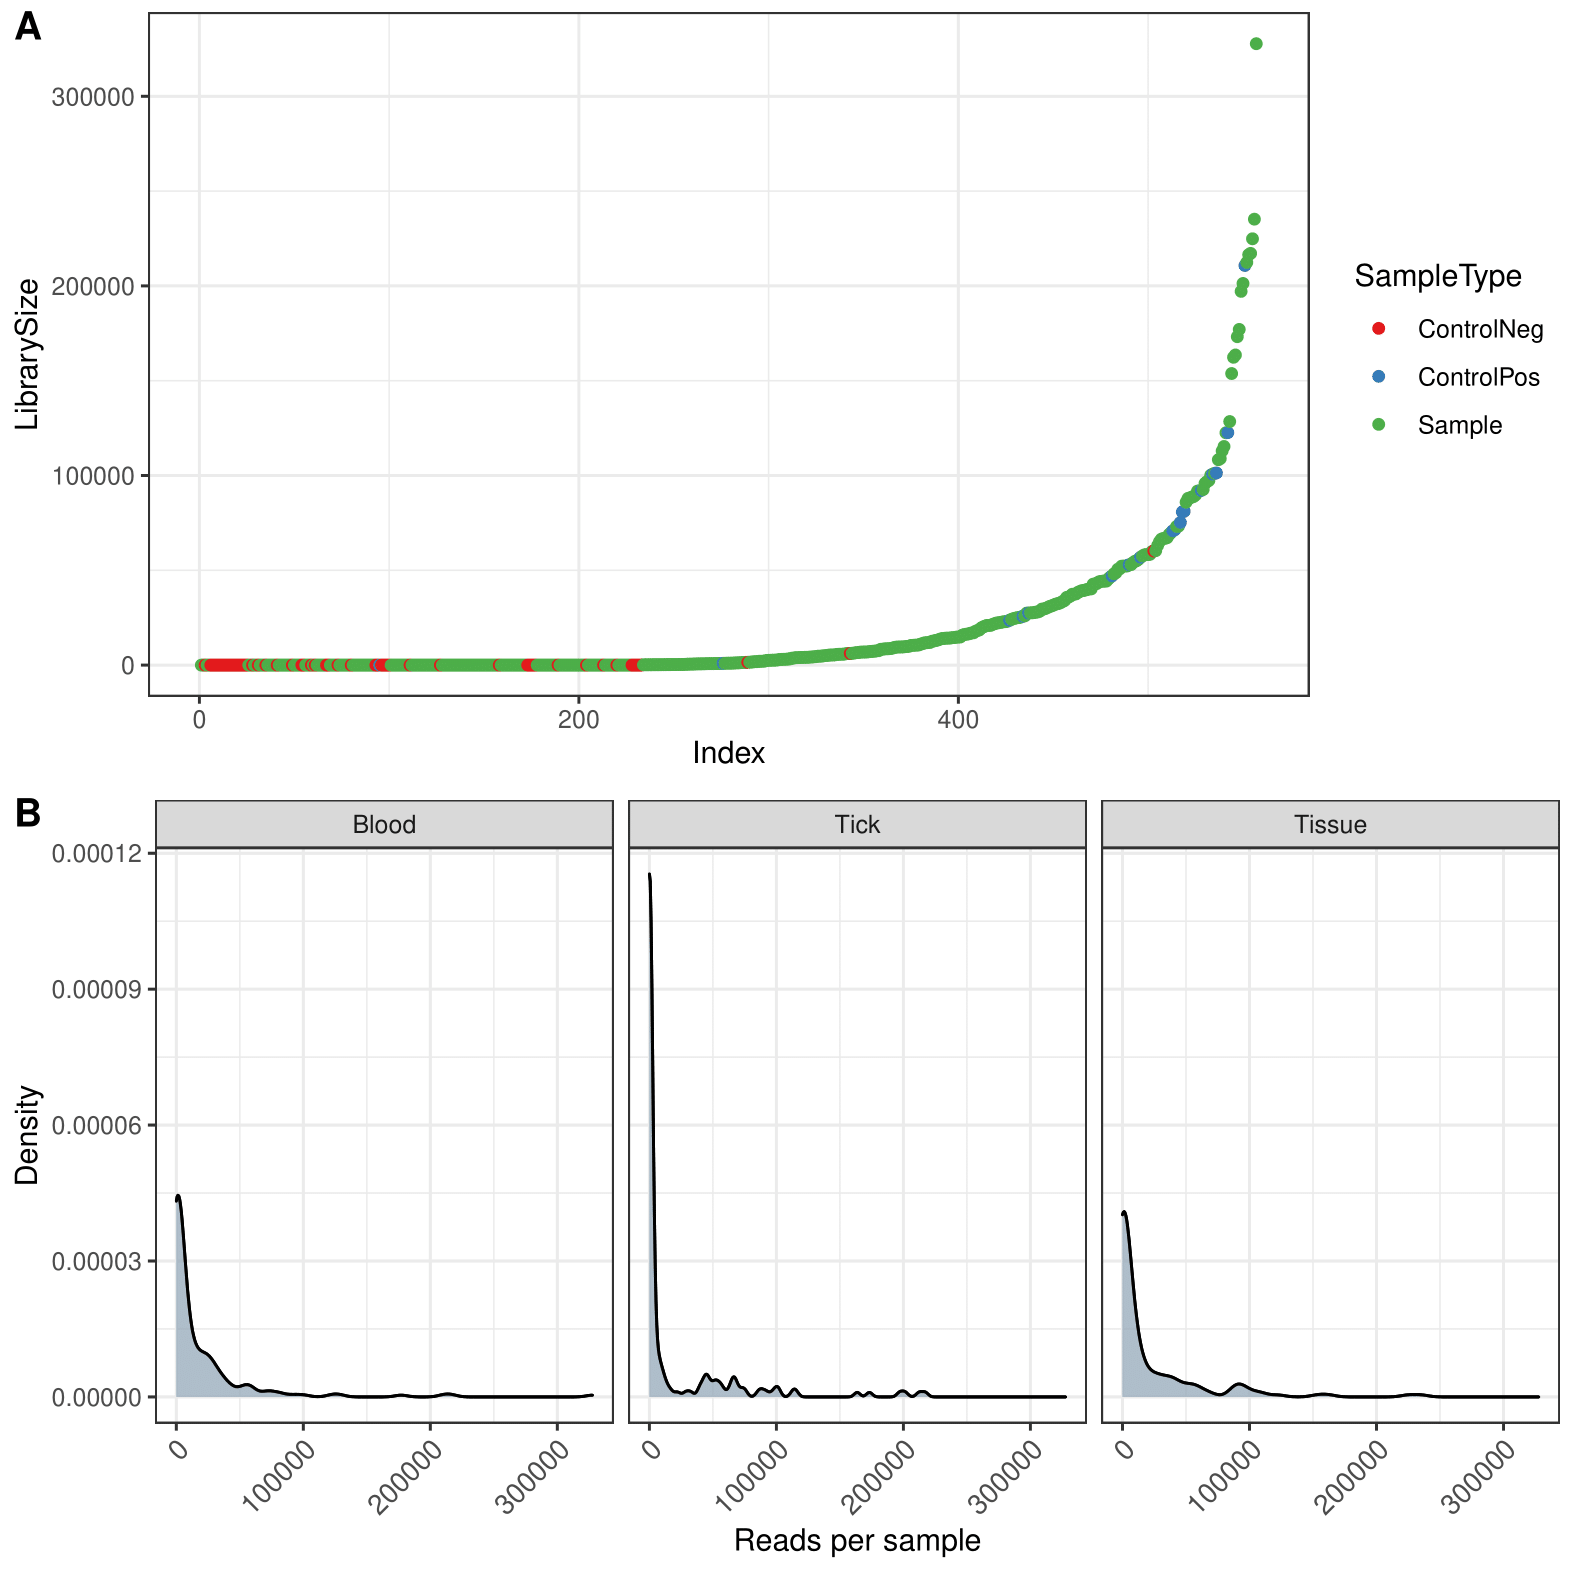
\includegraphics[width=0.95\linewidth]{figures/ms-figs-appendix/FigA-4.1} \caption[Sequence summary of trypanosome metabarcoding]{Summary of sequences obtained from trypanosome metabatcoding of the 18S rRNA gene. (A) Library size (i.e. number of sequences) obtained from samples. (B) Distribution of the number of reads in sample categories blood, tick and tissue.}\label{fig:FA41}
\end{figure}

\clearpage

\hypertarget{ch4-esupp}{%
\subsection{Supplementary Electronic Tables}\label{ch4-esupp}}

The following electronic supplementary files are available for download on \href{https://figshare.com/s/9eb3dba4096470af9904}{FigShare}, repository doi: 10.6084/m9.figshare.14370965.

\hypertarget{supplementary-table-e2.1}{%
\subsubsection{Supplementary table E2.1}\label{supplementary-table-e2.1}}

\textbf{Supplementary table E2.1:} \emph{Trypanosoma} amplicon sequence data from blood, tick and tissue samples. Data showing zOTUs belonging to the Trypanosomatidae family with results from NCBI BLAST analysis. \href{https://figshare.com/ndownloader/files/30578460}{Trypanosome zOTU taxonomy and sample data}

\hypertarget{supplementary-table-e2.2}{%
\subsubsection{Supplementary table E2.2}\label{supplementary-table-e2.2}}

\textbf{Supplementary table E2.2:} Genetic similarity of piroplasm sequences based on an 852 bp alignment of the 18S rRNA locus. Sequences generated from the present study in bold. Bottom half of matrix showing sequence similarity and top half containing genetic distance data.
\href{https://figshare.com/ndownloader/files/30578457}{Piroplasm genetic diversity table}

\hypertarget{supplementary-table-e2.3}{%
\subsubsection{Supplementary table E2.3}\label{supplementary-table-e2.3}}

\textbf{Supplementary table E2.3:} Genetic similarity of \emph{Hepatozoon} sequences based on an 819 bp alignment of the 18S rRNA locus. Sequences generated from the present study in bold. Bottom half of matrix showing sequence similarity and top half containing genetic distance data.
\href{https://figshare.com/ndownloader/files/30578463}{\emph{Hepatozoon} genetic diversity table}

\begin{center}\rule{0.5\linewidth}{0.5pt}\end{center}

\clearpage

\hypertarget{ch6-supp}{%
\section{Chapter 6}\label{ch6-supp}}

Supplementary material for Chapter \ref{tas-devil} on Tasmanian Devil Haemoprotozoa.

\begin{landscape}\begingroup\fontsize{8}{10}\selectfont

\begin{ThreePartTable}
\begin{TableNotes}
\item[a] Country abbreviations: AU - Australia, MZ - Mozambique, UK - United Kingdom, MY - Malaysia, SL - Sri Lanka, PNG - Papua New Guinea, DE - Germany, JP- Japan, PL- Poland, BR - Brazil, CA- Canada, PT - Portugal, US - United States of America. Australian states: QLD - Queensland, TAS - Tasmania, WA - Western Australia.
\item[b] Short sequences of the 18S rRNA gene only, included for comparison within the Trypanosoma cyclops clade.
\end{TableNotes}
\begin{longtabu} to \linewidth {>{}l>{\raggedright\arraybackslash}p{4cm}>{}l>{\raggedright\arraybackslash}p{3cm}>{\raggedright\arraybackslash}p{3cm}>{\raggedright\arraybackslash}p{3cm}}
\caption[Sequences used for phylogenetic analysis of \textit{Trypanosoma} in Tasmanian devils.]{\label{tab:TA61}\textit{Trypanosoma} sequences used in phylogenetic analysis in the present study. Sequences produced in the present study indicated in bold.}\\
\toprule
Species & Isolate & Host Scientific & Location (a) & 18S rRNA & gGAPDH\\
\midrule
\em{Tr. copemani} & JD-2008a Mika & \em{Koala (Phascolarctos cinereus)} & AU (NSW) & - & GU966585\\
\em{Tr. copemani} & JD-2008a Charlton & \em{Koala (Phascolarctos cinereus)} & AU (QLD) & GU966588 & -\\
\em{Tr. copemani} & TD-BRI115 & \em{Tasmanian devil (Sarcophilus harrisii)} & AU (TAS) & MT883297 & MT514664\\
\textbf{\em{Tr. copemani}} & \textbf{H26} & \textbf{\em{Wombat (Vombatus ursinus)}} & \textbf{AU (VIC)} & \textbf{AJ009169} & \textbf{}\\
\em{Tr. copemani} & G1 & \em{Woylie (Bettongia penicillata)} & AU (WA) & KC753530 & KC812982\\
\em{Tr. copemani} & APP & \em{Wombat (Vombatus ursinus)} & AU (VIC) & AJ620558 & AJ620277\\
\em{Tr. copemani} & G2 & \em{Woylie (Bettongia penicillata)} & AU (WA) & KC753531 & KC812983\\
\em{Tr. copemani} & Q2088 & \em{Quokka (Setonix brachyurus)} & AU (WA) & HQ267094 & HQ267095\\
\em{Tr. vegrandis} & G4 & \em{Woylie (Bettongia penicillata)} & AU (WA) & KC753532 & KC812985\\
\em{Tr. vegrandis} & G7 & \em{Woylie (Bettongia penicillata)} & AU (WA) & KC753536 & KC812987\\
\em{Tr. vegrandis} & G5 & \em{Woylie (Bettongia penicillata)} & AU (WA) & KC753534 & KC812986\\
\em{Tr. vegrandis} & G3 & \em{Woylie (Bettongia penicillata)} & AU (WA) & KC753533 & KC812984\\
\em{Tr. vegrandis} & G6 & \em{Woylie (Bettongia penicillata)} & AU (WA) & KC753535 & -\\
\em{Tr. gilletti} & Lanie & \em{Koala (Phascolarctos cinereus)} & AU (QLD) & GU966589 & GU966587\\
\em{Tr. cruzi} & G & \em{Opossum (Didelphis marsupialis)} & BR & AF239981 & GQ140351\\
\em{Tr. cruzi marinkellei} & TryCC 344 & \em{Bat (Carollia perspicillata)} & BR & FJ001664 & GQ140360\\
\em{Tr. erneyi} & TCC1294 & \em{Bat (Tadarida sp.)} & MZ & JN040988 & JN040965\\
\em{Tr. dionisii} & TryCC 211 & \em{Bat (Eptesicus brasiliensis)} & BR & FJ001666 & GQ140362\\
\em{Tr. rangeli} & AM80 & \em{Human (Homo sapiens)} & BR & AY491766 & JN040973\\
\em{Tr. noyesi} & H25 & \em{Kangaroo (Macropus giganteus)} & AU (VIC) & AJ009168 & AJ620276\\
\em{Tr. noyesi} & WC6218 & \em{Woylie (Bettongia penicillata)} & AU (WA) & KU354263 & KU354264\\
\em{Tr. livingstonei} & TCC1270 & \em{Bat (Rhinolophus landeri)} & MZ & KF192979 & KF192958\\
\em{Tr. lewisi} & Molteno B3 & \em{Rat (Rattus sp.)} & UK & AJ009156 & AJ629272\\
\em{Tr. microti} & TRL132 & \em{Vole (Microtis agrestis)} & UK & AJ009158 & AJ620273\\
\em{Tr. sp.} & TD-WPP601 (genotype A) & \em{Tasmanian devil (Sarcophilus harrisii)} & AU (TAS) & MT883326 & MT514665\\
\textbf{\em{Tr. sp.}} & \textbf{TD-WPP602 (genotype A)} & \textbf{\em{Tasmanian devil (Sarcophilus harrisii)}} & \textbf{AU (TAS)} & \textbf{-} & \textbf{MT514666}\\
\textbf{\em{Tr. sp.}} & \textbf{TD-WPP585 (genotype A)} & \textbf{\em{Tasmanian devil (Sarcophilus harrisii)}} & \textbf{AU (TAS)} & \textbf{MT883324} & \textbf{-}\\
\textbf{\em{Tr. sp.}} & \textbf{TD-BRI111 (genotype B)} & \textbf{\em{Tasmanian devil (Sarcophilus harrisii)}} & \textbf{AU (TAS)} & \textbf{MT883296} & \textbf{-}\\
\textbf{\em{Tr. sp.}} & \textbf{TD-TKN211 (genotype B)} & \textbf{\em{Tasmanian devil (Sarcophilus harrisii)}} & \textbf{AU (TAS)} & \textbf{MT883322} & \textbf{-}\\
\textbf{\em{Tr. sp.}} & \textbf{ABF (wallaby)} & \textbf{\em{Swamp wallaby (Wallabia bicolor)}} & \textbf{AU (VIC)} & \textbf{AJ620564} & \textbf{AJ620278}\\
\em{Tr. cyclops} & LV492 & \em{Macaque (Macaca sp.)} & MY & AJ131958 & FJ649493\\
\em{Tr. sp.} & TL.AQ.22 & \em{Leech(Philaemon)} & AU (QLD) & AJ620574 & AJ620280\\
\em{Tr. sp.} & TL.AQ.45 & \em{Leech(Philaemon)} & AU (QLD) & AJ620575 & -\\
\em{Tr. sp.} & TL.AV.44. cl157 & \em{Leech (Micobdella)} & AU (VIC) & AJ620573 & -\\
\em{Tr. sp.} & TL.AV.44 cl. 156B & \em{Leech (Micobdella)} & AU (VIC) & AJ620572 & -\\
\em{Tr. sp.} & TL.AV.43 cl100B & \em{Leech (Micobdella)} & AU (VIC) & AJ620570 & -\\
\em{Tr. sp.} & TL.AV.43 cl.101E & \em{Leech (Micobdella)} & AU (VIC) & AJ620571 & -\\
\em{Tr. sp.} & TL.AQ.40 & \em{Leech(Philaemon)} & AU (QLD) & AJ620576(b) & -\\
\em{Tr. sp.} & TL.AQ.48 & \em{Leech(Philaemon)} & AU (QLD) & AJ620577(b) & -\\
\em{Tr. sp.} & Frog ADE & \em{Frog (Mixophyes flaeyi)} & AU (VIC) & AJ620569(b) & -\\
\em{Tr. sp.} & TL.SL.1 & \em{Leech (Haemadipsa zeylanica)} & SL & AJ620578(b) & -\\
\em{Tr. sp.} & Wallaby 10 & \em{Brush-tailed rock-wallaby (Petrogale penicillate)} & AU (VIC) & AJ620563(b) & -\\
\em{Tr. sp.} & TL.NG.1 & \em{Leech (Leiobdella jawarerensis)} & PNG & AJ620581(b) & -\\
\em{Tr. theileri} & K127 & \em{Cattle (Bos taurus)} & DE & AJ009164 & AJ620282\\
\em{Tr. theileri} & KM & \em{Cattle (Bos taurus)} & JP & AB007814(b) & -\\
\em{Tr. theileri} & Bb756 & \em{European bison(Bison bonasus)} & PL & KF765801(b) & -\\
\em{Tr. theileri} & Tthc26 & \em{Cattle (Bos sp.)} & BR & GQ176153(b) & -\\
\em{Tr. irwini} &  & \em{Koala (Phascolarctos cinereus)} & AU (QLD, NSW) & FJ649479 & FJ649485\\
\em{Tr. bennetti} & KT-2 & \em{Kestrel (Falco sparverius)} & US & AJ223562 & FJ649486\\
\em{Tr. sp.} & ATT & \em{Currawong (Strepera sp.)} & AU (VIC) & AJ620557 & AJ620264\\
\em{Tr. mega} & ATCC 30038 & \em{Toad (Bufo regularis)} & Africa & AJ009157 & AJ620253\\
\em{Tr. rotatorium} & B2-II & \em{Bullfrog (Rana catesbeiana)} & CA & AJ009161 & AJ620256\\
\em{Tr. binneyi} & AWW & \em{Platypus (Ornithorhynchus anatinus)} & AU (VIC) & AJ620565 & AJ620266\\
\em{Tr. granulosum} & UK & \em{Eel (Anguilla anguilla)} & PT & AJ620551 & -\\
\em{Phytomonas serpens} & N/A & \em{N/A} & N/A & U39577 & EU084892\\
\em{Herpetomonas muscarum} & N/A & \em{N/A} & N/A & L18872 & DQ092548\\
\bottomrule
\insertTableNotes
\end{longtabu}
\end{ThreePartTable}
\endgroup{}
\end{landscape}

\begin{landscape}\begingroup\fontsize{8.5}{10.5}\selectfont

\begin{longtable}[t]{>{}rlrrrrrrrrrrrrrrrrrrrrl}
\caption[Pairwise genetic similarity matrix of the \textit{Trypanosoma cyclops} clade.]{\label{tab:TA62}Pairwise genetic similarity matrix of the \textit{Trypanosoma cyclops} clade from sequences at the 18S rRNA gene. Analysis conducted over at 559 bp alignment of the V7-8 hypervariable using the Kimura Two-Parameter (K2P) method.}\\
\toprule
 & Genotype & 1 & 2 & 3 & 4 & 5 & 6 & 7 & 8 & 9 & 10 & 11 & 12 & 13 & 14 & 15 & 16 & 17 & 18 & 19 & 20 & 21\\
\midrule
\em{1} & T. theileri KM AB007814 &  &  &  &  &  &  &  &  &  &  &  &  &  &  &  &  &  &  &  &  & \\
\em{2} & T. theileri Bb756 KF765801 & 100.0 &  &  &  &  &  &  &  &  &  &  &  &  &  &  &  &  &  &  &  & \\
\em{3} & T. theileri K127 AJ009164 & 97.5 & 97.5 &  &  &  &  &  &  &  &  &  &  &  &  &  &  &  &  &  &  & \\
\em{4} & T. theileri Tthc26 GQ176153 & 97.2 & 97.2 & 99.8 &  &  &  &  &  &  &  &  &  &  &  &  &  &  &  &  &  & \\
\em{5} & T. sp. TL.AQ.40 AJ620576 & 87.3 & 87.3 & 87.2 & 87.5 &  &  &  &  &  &  &  &  &  &  &  &  &  &  &  &  & \\
\em{6} & T. sp. TL.AQ.48 AJ620577 & 87.3 & 87.3 & 87.2 & 87.5 & 99.8 &  &  &  &  &  &  &  &  &  &  &  &  &  &  &  & \\
\em{7} & T. sp. Frog ADE AJ620569 & 87.4 & 87.4 & 87.3 & 87.5 & 95.3 & 95.1 &  &  &  &  &  &  &  &  &  &  &  &  &  &  & \\
\em{8} & T. cyclops LV492 AJ131958 & 82.2 & 82.2 & 82.2 & 82.4 & 89.6 & 89.3 & 88.1 &  &  &  &  &  &  &  &  &  &  &  &  &  & \\
\em{9} & T. sp. TL.AQ.45 AJ620575 & 88.2 & 88.2 & 88.2 & 88.4 & 97.2 & 97.0 & 98.1 & 89.8 &  &  &  &  &  &  &  &  &  &  &  &  & \\
\em{10} & WPP585 MT883324 & 82.0 & 82.0 & 82.0 & 82.2 & 90.7 & 90.4 & 89.4 & 97.4 & 91.1 &  &  &  &  &  &  &  &  &  &  &  & \\
\em{11} & WPP601 MT883326 & 82.0 & 82.0 & 82.0 & 82.2 & 90.7 & 90.4 & 89.4 & 97.4 & 91.1 & 100.0 &  &  &  &  &  &  &  &  &  &  & \\
\em{12} & BRI111 MT883296 & 87.0 & 87.0 & 87.0 & 87.2 & 96.9 & 96.7 & 97.0 & 89.5 & 98.4 & 90.9 & 90.9 &  &  &  &  &  &  &  &  &  & \\
\em{13} & T. sp. TL.AQ.22 AJ620574 & 82.0 & 82.0 & 82.0 & 82.2 & 89.8 & 89.6 & 88.8 & 97.2 & 90.5 & 98.5 & 98.5 & 90.2 &  &  &  &  &  &  &  &  & \\
\em{14} & T. sp. TL.AV.44 cl157 AJ620573 & 87.2 & 87.2 & 87.1 & 87.4 & 95.6 & 95.4 & 98.4 & 88.8 & 98.4 & 89.7 & 89.7 & 97.2 & 89.1 &  &  &  &  &  &  &  & \\
\em{15} & T. sp. TL.SL.1 AJ620578 & 86.8 & 86.8 & 86.7 & 86.9 & 95.4 & 95.2 & 98.1 & 88.2 & 98.1 & 89.5 & 89.5 & 97.0 & 88.9 & 99.3 &  &  &  &  &  &  & \\
\em{16} & T. sp. ABF AJ620564 & 87.5 & 87.5 & 87.5 & 87.7 & 97.7 & 97.4 & 97.4 & 90.4 & 98.8 & 90.9 & 90.9 & 98.1 & 90.7 & 97.2 & 97.0 &  &  &  &  &  & \\
\em{17} & T. sp. TL.AV.44 cl158b AJ620572 & 87.1 & 87.1 & 87.0 & 87.2 & 95.4 & 95.2 & 97.2 & 88.3 & 98.2 & 89.6 & 89.6 & 96.5 & 89.0 & 98.4 & 98.2 & 97.0 &  &  &  &  & \\
\em{18} & T. sp. TL.AV.43 cl100b AJ620570 & 88.2 & 88.2 & 88.2 & 88.4 & 95.6 & 95.3 & 96.7 & 88.7 & 98.4 & 89.6 & 89.6 & 96.7 & 89.0 & 97.4 & 96.8 & 97.2 & 97.0 &  &  &  & \\
\em{19} & T. sp. TL.AV.43 cl100e AJ620571 & 88.7 & 88.7 & 88.6 & 88.8 & 96.3 & 96.0 & 97.4 & 89.0 & 99.1 & 90.3 & 90.3 & 97.4 & 89.7 & 97.7 & 97.5 & 97.9 & 97.7 & 99.3 &  &  & \\
\em{20} & T. sp. wallaby 10 AJ620563 & 88.4 & 88.4 & 88.4 & 88.6 & 96.0 & 95.8 & 97.2 & 88.7 & 98.8 & 90.0 & 90.0 & 97.2 & 89.4 & 97.4 & 97.2 & 97.7 & 97.5 & 99.1 & 99.8 &  & \\
\em{21} & T. sp. TL.NG.1 AJ620581 & 90.5 & 90.5 & 90.0 & 90.0 & 96.0 & 95.7 & 96.8 & 87.5 & 98.7 & 88.7 & 88.7 & 96.8 & 88.0 & 97.1 & 96.8 & 97.6 & 97.4 & 98.9 & 99.7 & 100 & \\
\bottomrule
\end{longtable}
\endgroup{}
\end{landscape}


%%%%% REFERENCES
\setlength{\baselineskip}{0pt} % JEM: Single-space References
\setquotestyle{english}
\DeclareFieldFormat[inbook,thesis,article]{title}{\mkbibemph{#1}\addperiod} % italic title with period
\renewbibmacro{in:}{} % remove the word in before journal title
\renewbibmacro{en.}{} % remove the word in before journal title
\DeclareFieldFormat{journaltitle}{\textbf{#1}\addcomma} % bold journal title with comma
\DeclareFieldFormat[article]{volume}{{#1}\addcolon\space}
\printbibliography[heading=bibintoc,title={\bibtitle}]


\end{document}
